% JASA manuscript adaptation of the user-supplied JASA_template_2025.
% Based on template.tex (article 12pt, natbib+agsm, \spacingset{1.8}).
% Source of scientific text: Id_prob_and_QMLE_CP_model_AOS (5).zip.
% ASA review guideline overrides template's extra-large text area: US Letter, 1in margins.
\documentclass[12pt,letterpaper]{article}
\usepackage[T1]{fontenc}
\usepackage[utf8]{inputenc}
\usepackage{lmodern}
\usepackage{amsmath,amssymb,amsfonts,amsthm,mathtools}
\usepackage{graphicx,booktabs,multirow,threeparttable,adjustbox,mathrsfs,bm}
\usepackage{algorithm,algpseudocode}
\usepackage[authoryear]{natbib}
\usepackage{geometry}
\geometry{paper=letterpaper,margin=1in}
\usepackage{microtype}
\usepackage{float}
\usepackage{placeins}
\usepackage{url}
\usepackage[hidelinks]{hyperref}
\usepackage{bookmark}
\setlength{\emergencystretch}{3em}
\sloppy
% Preserve the user-supplied template's spacing macro exactly.
\def\spacingset#1{\renewcommand{\baselinestretch}{#1}\small\normalsize}
% User-supplied template: anon=0 hides authors; anon=1 displays them.
\providecommand{\anon}{0}
\providecommand{\compactreferences}{1}
\bibliographystyle{agsm_jasa_refs}
\theoremstyle{plain}
\newtheorem{theorem}{Theorem}
\newtheorem{proposition}[theorem]{Proposition}
\newtheorem{lemma}[theorem]{Lemma}
\newtheorem{corollary}[theorem]{Corollary}
\theoremstyle{definition}
\newtheorem{example}{Example}
\newtheorem{remark}{Remark}
\newtheorem{definition}{Definition}
\newtheorem{assumption}{Assumption}
\renewcommand{\theassumption}{A\arabic{assumption}}
\newcommand{\Assumption}[1][]{\begin{assumption}[#1]}
\newcommand{\EndAssumption}{\end{assumption}}
\DeclareMathOperator{\vech}{vech}
\newcommand{\R}{\mathbb{R}}
\newcommand{\diag}{\operatorname{diag}}
\newcommand{\rank}{\operatorname{rank}}
\newcommand{\Span}{\operatorname{Span}}
\newcommand{\Mat}{\mathrm{Mat}}
\newcommand{\GL}{\mathrm{GL}}
\newcommand{\Id}{I}
\newcommand{\odotKR}{\odot} \newcommand{\KR}{\odot}
\newcommand{\ot}{\otimes}
\newcommand{\Dim}{\operatorname{dim}}
\newcommand{\Dgroup}{D_d}
\newcommand{\Sgroup}{S_d}
\renewcommand{\figurename}{Figure}
\renewcommand{\tablename}{Table}

\newtheorem{proofcondition}{Proof condition}
\renewcommand{\theproofcondition}{D.\arabic{proofcondition}}
\providecommand{\tr}{\operatorname{tr}}
\providecommand{\Diag}{\operatorname{Diag}}
\providecommand{\op}{\operatorname{op}}
\providecommand{\vecop}{\operatorname{vec}}
\providecommand{\cD}{\mathcal D}
\providecommand{\cM}{\mathcal M}
\providecommand{\cW}{\mathcal W}
\providecommand{\cR}{\mathcal R}
\providecommand{\norm}[1]{\left\lVert #1\right\rVert}
\providecommand{\ip}[2]{\left\langle #1,#2\right\rangle}
\providecommand{\Zh}{\widehat Z}
\providecommand{\Mh}{\widehat M_x}
\providecommand{\Seh}{\widehat\Sigma_e}
\providecommand{\Syh}{\widehat\Sigma_y}
\providecommand{\Ph}{\widehat P}
\providecommand{\Sh}{\widehat{\mathscr S}}
\providecommand{\Gh}{\widehat G_H}
\allowdisplaybreaks[1]
\providecommand{\bseriesno}[1]{#1}
\renewcommand{\thesection}{D.\arabic{section}}
\renewcommand{\theequation}{D.\arabic{equation}}
\renewcommand{\thefigure}{D.\arabic{figure}}
\renewcommand{\thetable}{D.\arabic{table}}
\renewcommand{\thetheorem}{D.\arabic{theorem}}
\renewcommand{\theexample}{D.\arabic{example}}
\renewcommand{\theremark}{D.\arabic{remark}}
\renewcommand{\thealgorithm}{D.\arabic{algorithm}}

\begin{document}
\spacingset{1}
\hypersetup{pdftitle={Supplementary numerical data for the CP-factor model}}
\title{\bfseries Supplementary Numerical Data\\[4pt]
\large Identification problem and quasi-maximum likelihood estimation
for matrix-variate CP-factor models}
\author{}
\date{}
\maketitle
\noindent This file contains the complete numerical listings and extended
diagnostic discussion accompanying Subsection~S.2.3 of the Supplementary
Material. The Supplementary Material retains the diagnostic definitions,
experimental design and core finite-sample comparisons. Sections~D.1--D.4
collect the complete tables, figures and archived comparisons; Section~D.5
contains the extended interpretation, selected summaries, denominator
diagnostics and additional-iteration sensitivity. Section~D.6
collects ancillary AUC comparisons of the early finite samples.
No estimates, diagnostics, means, variances or AUCs have been changed
in preparing this separate data file.

\medskip\noindent The primary searches use the fitted unit-column cores
$A_r,B_r$ and $m_r(\lambda)=A_r\operatorname{diag}(\lambda)B_r^\top$,
with $\|m_r(\lambda)\|_F=1$ and
$\max_j|\lambda_j|/\|\lambda\|_2\le0.90$.
The latter excludes a $25.84^\circ$ neighborhood of every coefficient axis;
it does not impose a matrix-loading cosine cutoff. The local coefficient-angle
caps have radii $5^\circ$ and $10^\circ$.
Each bracket reports a sample variance, not a standard deviation.
$E_1$ and all Jacobian singular values are unsquared; $E_1$ is not
multiplied by 100. The numerical polynomial ratio is
$\rho_{\mathrm{ind}}=\rho/2$, using each distinct minor once.
The nine dimension pairs and four sample sizes give 108 cells and
10,796 available estimates; the interior $80\times80$, $T=100$ cell
has 96 estimates, and every other cell has 100.
The archived matrix-angle experiment is separated at the end.

\tableofcontents
\clearpage
\section{Complete coefficient-angle-domain tables}
\par\medskip\noindent\textit{Index to the complete coefficient-angle-domain grid.}
\begingroup
\spacingset{1.0}
\small\begin{center}
\begin{tabular}{crrrrrrr}
\toprule
& \multicolumn{3}{c}{Metric tables} & \multicolumn{3}{c}{Spectrum tables} & AUC\\
$(p,q)$ & $I$ & $B$ & $E$ & $I$ (first part) & $B$ & $E$ & All $T$\\
\midrule
$(20,20)$ & \ref{s23:lambda:alltab:metrics:p20q20interior} & \ref{s23:lambda:alltab:metrics:p20q20boundary} & \ref{s23:lambda:alltab:metrics:p20q20exterior} & \ref{s23:lambda:alltab:spectra:p20q20interior:1-3} & \ref{s23:lambda:alltab:spectra:p20q20boundary:1-5} & \ref{s23:lambda:alltab:spectra:p20q20exterior:1-5} & \ref{s23:lambda:allauc:p20q20}\\
$(20,40)$ & \ref{s23:lambda:alltab:metrics:p20q40interior} & \ref{s23:lambda:alltab:metrics:p20q40boundary} & \ref{s23:lambda:alltab:metrics:p20q40exterior} & \ref{s23:lambda:alltab:spectra:p20q40interior:1-3} & \ref{s23:lambda:alltab:spectra:p20q40boundary:1-5} & \ref{s23:lambda:alltab:spectra:p20q40exterior:1-5} & \ref{s23:lambda:allauc:p20q40}\\
$(20,80)$ & \ref{s23:lambda:alltab:metrics:p20q80interior} & \ref{s23:lambda:alltab:metrics:p20q80boundary} & \ref{s23:lambda:alltab:metrics:p20q80exterior} & \ref{s23:lambda:alltab:spectra:p20q80interior:1-3} & \ref{s23:lambda:alltab:spectra:p20q80boundary:1-5} & \ref{s23:lambda:alltab:spectra:p20q80exterior:1-5} & \ref{s23:lambda:allauc:p20q80}\\
$(40,20)$ & \ref{s23:lambda:alltab:metrics:p40q20interior} & \ref{s23:lambda:alltab:metrics:p40q20boundary} & \ref{s23:lambda:alltab:metrics:p40q20exterior} & \ref{s23:lambda:alltab:spectra:p40q20interior:1-3} & \ref{s23:lambda:alltab:spectra:p40q20boundary:1-5} & \ref{s23:lambda:alltab:spectra:p40q20exterior:1-5} & \ref{s23:lambda:allauc:p40q20}\\
$(40,40)$ & \ref{s23:lambda:alltab:metrics:p40q40interior} & \ref{s23:lambda:alltab:metrics:p40q40boundary} & \ref{s23:lambda:alltab:metrics:p40q40exterior} & \ref{s23:lambda:alltab:spectra:p40q40interior:1-3} & \ref{s23:lambda:alltab:spectra:p40q40boundary:1-5} & \ref{s23:lambda:alltab:spectra:p40q40exterior:1-5} & \ref{s23:lambda:allauc:p40q40}\\
$(40,80)$ & \ref{s23:lambda:alltab:metrics:p40q80interior} & \ref{s23:lambda:alltab:metrics:p40q80boundary} & \ref{s23:lambda:alltab:metrics:p40q80exterior} & \ref{s23:lambda:alltab:spectra:p40q80interior:1-3} & \ref{s23:lambda:alltab:spectra:p40q80boundary:1-5} & \ref{s23:lambda:alltab:spectra:p40q80exterior:1-5} & \ref{s23:lambda:allauc:p40q80}\\
$(80,20)$ & \ref{s23:lambda:alltab:metrics:p80q20interior} & \ref{s23:lambda:alltab:metrics:p80q20boundary} & \ref{s23:lambda:alltab:metrics:p80q20exterior} & \ref{s23:lambda:alltab:spectra:p80q20interior:1-3} & \ref{s23:lambda:alltab:spectra:p80q20boundary:1-5} & \ref{s23:lambda:alltab:spectra:p80q20exterior:1-5} & \ref{s23:lambda:allauc:p80q20}\\
$(80,40)$ & \ref{s23:lambda:alltab:metrics:p80q40interior} & \ref{s23:lambda:alltab:metrics:p80q40boundary} & \ref{s23:lambda:alltab:metrics:p80q40exterior} & \ref{s23:lambda:alltab:spectra:p80q40interior:1-3} & \ref{s23:lambda:alltab:spectra:p80q40boundary:1-5} & \ref{s23:lambda:alltab:spectra:p80q40exterior:1-5} & \ref{s23:lambda:allauc:p80q40}\\
$(80,80)$ & \ref{s23:lambda:alltab:metrics:p80q80interior} & \ref{s23:lambda:alltab:metrics:p80q80boundary} & \ref{s23:lambda:alltab:metrics:p80q80exterior} & \ref{s23:lambda:alltab:spectra:p80q80interior:1-3} & \ref{s23:lambda:alltab:spectra:p80q80boundary:1-5} & \ref{s23:lambda:alltab:spectra:p80q80exterior:1-5} & \ref{s23:lambda:allauc:p80q80}\\
\bottomrule
\end{tabular}\end{center}\endgroup
\noindent All metric and spectrum groups report $T=100,200,400,800$. Interior spectra continue for $\ell=4$--$6$ and $7$--$8$ in the next two tables. $I$, $B$, and $E$ denote the three designs. The Jacobian spectra depend only on the unchanged fitted loadings; all off-axis geometric scores use $\mathcal D^\lambda_{\delta_0}$.

% Complete new lambda-domain geometry; archived fit-only Jacobians are reused unchanged.
\clearpage
\begin{table}[p]
\begingroup
\spacingset{1.0}
\small\centering
\caption{Complete diagnostics on $\mathcal D^\lambda_{\delta_0}$: identifiable interior, $p=20$, $q=20$. Panels A--B report mean [sample variance]; Panel C gives the actual denominators and contacts.}
\label{s23:lambda:alltab:metrics:p20q20interior}
\footnotesize
\setlength{\tabcolsep}{3.5pt}
\renewcommand{\arraystretch}{0.96}
\scriptsize
\begin{adjustbox}{max width=\linewidth}
\begin{tabular}{@{}lcccc@{}}
\toprule
Metric & $T=100$ & $T=200$ & $T=400$ & $T=800$\\
\midrule
\multicolumn{5}{@{}l}{\textit{Panel A: polynomial and rank-one residuals}}\\
$\rho_{\mathrm{ind},\min}$ & \shortstack{0.059290\\[-1pt]{\scriptsize[1.72e-05]}} & \shortstack{0.057250\\[-1pt]{\scriptsize[7.81e-06]}} & \shortstack{0.056287\\[-1pt]{\scriptsize[3.07e-06]}} & \shortstack{0.055859\\[-1pt]{\scriptsize[1.69e-06]}}\\
$E_{1,\mathrm{center}}$ & \shortstack{0.045119\\[-1pt]{\scriptsize[2.31e-05]}} & \shortstack{0.043306\\[-1pt]{\scriptsize[1.02e-05]}} & \shortstack{0.042452\\[-1pt]{\scriptsize[4.35e-06]}} & \shortstack{0.042206\\[-1pt]{\scriptsize[2.17e-06]}}\\
$E_{1,5}$ & \shortstack{0.041907\\[-1pt]{\scriptsize[1.81e-05]}} & \shortstack{0.040287\\[-1pt]{\scriptsize[8.14e-06]}} & \shortstack{0.039540\\[-1pt]{\scriptsize[3.51e-06]}} & \shortstack{0.039351\\[-1pt]{\scriptsize[1.76e-06]}}\\
$E_{1,10}$ & \shortstack{0.039829\\[-1pt]{\scriptsize[1.69e-05]}} & \shortstack{0.038318\\[-1pt]{\scriptsize[7.63e-06]}} & \shortstack{0.037638\\[-1pt]{\scriptsize[3.32e-06]}} & \shortstack{0.037504\\[-1pt]{\scriptsize[1.67e-06]}}\\
$\rho_{\mathrm{ind}}$ at the $10^\circ$ solution & \shortstack{0.062475\\[-1pt]{\scriptsize[1.89e-05]}} & \shortstack{0.060398\\[-1pt]{\scriptsize[8.63e-06]}} & \shortstack{0.059427\\[-1pt]{\scriptsize[3.43e-06]}} & \shortstack{0.059028\\[-1pt]{\scriptsize[1.91e-06]}}\\
Independent $(E_1)_{\min}$ & \shortstack{0.028883\\[-1pt]{\scriptsize[5.31e-06]}} & \shortstack{0.028092\\[-1pt]{\scriptsize[2.57e-06]}} & \shortstack{0.027783\\[-1pt]{\scriptsize[1.19e-06]}} & \shortstack{0.027768\\[-1pt]{\scriptsize[6.09e-07]}}\\
$\rho_{\mathrm{ind}}$ at independent $(E_1)_{\min}$ & \shortstack{0.076810\\[-1pt]{\scriptsize[3.58e-05]}} & \shortstack{0.074844\\[-1pt]{\scriptsize[1.58e-05]}} & \shortstack{0.074001\\[-1pt]{\scriptsize[7.71e-06]}} & \shortstack{0.074005\\[-1pt]{\scriptsize[4.02e-06]}}\\
$E_{1,5}-E_{1,10}$ & \shortstack{0.002078\\[-1pt]{\scriptsize[3.52e-07]}} & \shortstack{0.001969\\[-1pt]{\scriptsize[1.64e-07]}} & \shortstack{0.001902\\[-1pt]{\scriptsize[6.34e-08]}} & \shortstack{0.001847\\[-1pt]{\scriptsize[3.52e-08]}}\\
\addlinespace[2pt]
\multicolumn{5}{@{}l}{\textit{Panel B: local geometry, correspondence and recovery}}\\
$j_{\mathrm{orig}}$ & \shortstack{0.089019\\[-1pt]{\scriptsize[2.35e-05]}} & \shortstack{0.088129\\[-1pt]{\scriptsize[1.06e-05]}} & \shortstack{0.087469\\[-1pt]{\scriptsize[4.79e-06]}} & \shortstack{0.087040\\[-1pt]{\scriptsize[2.39e-06]}}\\
$j_{\mathrm{nor}}$ & \shortstack{0.063416\\[-1pt]{\scriptsize[1.46e-05]}} & \shortstack{0.062562\\[-1pt]{\scriptsize[6.87e-06]}} & \shortstack{0.062006\\[-1pt]{\scriptsize[3.05e-06]}} & \shortstack{0.061650\\[-1pt]{\scriptsize[1.42e-06]}}\\
$Q_T(5^\circ)$, finite values & \shortstack{0.111726\\[-1pt]{\scriptsize[6.75e-05]}} & \shortstack{0.110489\\[-1pt]{\scriptsize[6.12e-05]}} & \shortstack{0.109780\\[-1pt]{\scriptsize[4.89e-05]}} & \shortstack{0.109275\\[-1pt]{\scriptsize[3.73e-06]}}\\
$\Delta_T$ (degrees) & \shortstack{27.319\\[-1pt]{\scriptsize[7.09e+00]}} & \shortstack{28.245\\[-1pt]{\scriptsize[2.30e+00]}} & \shortstack{28.464\\[-1pt]{\scriptsize[1.08e+00]}} & \shortstack{28.472\\[-1pt]{\scriptsize[7.45e-01]}}\\
Center-to-$10^\circ$ solution angle (degrees) & \shortstack{10.000\\[-1pt]{\scriptsize[3.29e-17]}} & \shortstack{10.000\\[-1pt]{\scriptsize[4.14e-17]}} & \shortstack{10.000\\[-1pt]{\scriptsize[2.89e-17]}} & \shortstack{10.000\\[-1pt]{\scriptsize[3.39e-17]}}\\
Local $E_1$ within $10^\circ$, conditional & \shortstack{0.050203\\[-1pt]{\scriptsize[\text{NA}]}} & \textemdash & \textemdash & \textemdash\\
Physical $c_{\mathrm{mat}}$ at independent $(E_1)_{\min}$ & \shortstack{0.977169\\[-1pt]{\scriptsize[3.80e-05]}} & \shortstack{0.977905\\[-1pt]{\scriptsize[3.65e-07]}} & \shortstack{0.977902\\[-1pt]{\scriptsize[1.83e-07]}} & \shortstack{0.977861\\[-1pt]{\scriptsize[9.27e-08]}}\\
Physical $c_{\mathrm{mat}}$ at $E_{1,10}$ & \shortstack{0.914300\\[-1pt]{\scriptsize[5.70e-04]}} & \shortstack{0.919559\\[-1pt]{\scriptsize[6.71e-05]}} & \shortstack{0.920030\\[-1pt]{\scriptsize[2.82e-05]}} & \shortstack{0.919401\\[-1pt]{\scriptsize[1.40e-05]}}\\
$e_Z$ & \shortstack{0.031163\\[-1pt]{\scriptsize[1.54e-05]}} & \shortstack{0.021606\\[-1pt]{\scriptsize[7.27e-06]}} & \shortstack{0.015027\\[-1pt]{\scriptsize[3.44e-06]}} & \shortstack{0.010598\\[-1pt]{\scriptsize[1.58e-06]}}\\
$e_\Sigma$ & \shortstack{0.251016\\[-1pt]{\scriptsize[5.94e-03]}} & \shortstack{0.176778\\[-1pt]{\scriptsize[2.13e-03]}} & \shortstack{0.121848\\[-1pt]{\scriptsize[7.32e-04]}} & \shortstack{0.084718\\[-1pt]{\scriptsize[3.30e-04]}}\\
\addlinespace[2pt]
\multicolumn{5}{@{}l}{\textit{Panel C: denominators and constraint contacts}}\\
Available estimates & 100 & 100 & 100 & 100\\
Finite $Q_T$ / available & 100/100 & 100/100 & 100/100 & 100/100\\
Found local candidate / available & 1/100 & 0/100 & 0/100 & 0/100\\
Independent $\Delta_T\le5^\circ$ / available & 0/100 & 0/100 & 0/100 & 0/100\\
Strict QMLE stopping / available & 25/100 & 43/100 & 53/100 & 67/100\\
$10^\circ$ angular-cap contact / available & 100/100 & 100/100 & 100/100 & 100/100\\
$\lambda$-axis exclusion contact / available & 0/100 & 0/100 & 0/100 & 0/100\\
Auxiliary $c_{\mathrm{mat}}>0.90$ at $E_{1,10}$ / available & 89/100 & 100/100 & 100/100 & 100/100\\
\bottomrule
\end{tabular}
\end{adjustbox}
\par\smallskip
\begin{minipage}{0.98\linewidth}\footnotesize
All geometric searches use $\max_j|\lambda_j|/\|\lambda\|\le0.90$ and projective coefficient angles. Physical $c_{\mathrm{mat}}$ values are auxiliary diagnostics and may exceed $0.90$. Subscripts $\min$ denote the lowest feasible candidates found; numerical stopping does not certify mathematical local or global optimality. $\rho_{\mathrm{ind}}=\rho/2$; $J$ uses the $\psi$-column convention. $Q_T$ and conditional local $E_1$ use only finite/found cases; unmatched $Q_T=+\infty$ is retained. A dash means no found value; NA means variance unavailable at fewer than two values. Variances use actual counts minus one. No imputation or strict-stopping filter is applied. QMLE estimates and budgets are unchanged; only geometric searches are new.
\end{minipage}
\endgroup
\end{table}
\clearpage
\begin{table}[p]
\begingroup
\spacingset{1.0}
\small\centering
\caption{Complete diagnostics on $\mathcal D^\lambda_{\delta_0}$: identifiable boundary, $p=20$, $q=20$. Panels A--B report mean [sample variance]; Panel C gives the actual denominators and contacts.}
\label{s23:lambda:alltab:metrics:p20q20boundary}
\footnotesize
\setlength{\tabcolsep}{3.5pt}
\renewcommand{\arraystretch}{0.96}
\scriptsize
\begin{adjustbox}{max width=\linewidth}
\begin{tabular}{@{}lcccc@{}}
\toprule
Metric & $T=100$ & $T=200$ & $T=400$ & $T=800$\\
\midrule
\multicolumn{5}{@{}l}{\textit{Panel A: polynomial and rank-one residuals}}\\
$\rho_{\mathrm{ind},\min}$ & \shortstack{0.017666\\[-1pt]{\scriptsize[1.59e-05]}} & \shortstack{0.013211\\[-1pt]{\scriptsize[7.34e-06]}} & \shortstack{0.009839\\[-1pt]{\scriptsize[3.13e-06]}} & \shortstack{0.007546\\[-1pt]{\scriptsize[2.45e-06]}}\\
$E_{1,\mathrm{center}}$ & \shortstack{0.027415\\[-1pt]{\scriptsize[3.19e-04]}} & \shortstack{0.012622\\[-1pt]{\scriptsize[2.88e-05]}} & \shortstack{0.007316\\[-1pt]{\scriptsize[6.75e-06]}} & \shortstack{0.004340\\[-1pt]{\scriptsize[1.08e-06]}}\\
$E_{1,5}$ & \shortstack{0.022122\\[-1pt]{\scriptsize[1.66e-04]}} & \shortstack{0.010694\\[-1pt]{\scriptsize[1.69e-05]}} & \shortstack{0.006443\\[-1pt]{\scriptsize[3.75e-06]}} & \shortstack{0.004054\\[-1pt]{\scriptsize[7.81e-07]}}\\
$E_{1,10}$ & \shortstack{0.018543\\[-1pt]{\scriptsize[9.55e-05]}} & \shortstack{0.009439\\[-1pt]{\scriptsize[1.07e-05]}} & \shortstack{0.005920\\[-1pt]{\scriptsize[2.25e-06]}} & \shortstack{0.003977\\[-1pt]{\scriptsize[6.85e-07]}}\\
$\rho_{\mathrm{ind}}$ at the $10^\circ$ solution & \shortstack{0.018337\\[-1pt]{\scriptsize[1.41e-05]}} & \shortstack{0.013735\\[-1pt]{\scriptsize[6.36e-06]}} & \shortstack{0.010278\\[-1pt]{\scriptsize[2.66e-06]}} & \shortstack{0.007753\\[-1pt]{\scriptsize[2.14e-06]}}\\
Independent $(E_1)_{\min}$ & \shortstack{0.010646\\[-1pt]{\scriptsize[4.17e-06]}} & \shortstack{0.007588\\[-1pt]{\scriptsize[1.97e-06]}} & \shortstack{0.005443\\[-1pt]{\scriptsize[8.80e-07]}} & \shortstack{0.003942\\[-1pt]{\scriptsize[5.89e-07]}}\\
$\rho_{\mathrm{ind}}$ at independent $(E_1)_{\min}$ & \shortstack{0.021047\\[-1pt]{\scriptsize[1.61e-05]}} & \shortstack{0.015047\\[-1pt]{\scriptsize[7.58e-06]}} & \shortstack{0.010828\\[-1pt]{\scriptsize[3.43e-06]}} & \shortstack{0.007870\\[-1pt]{\scriptsize[2.38e-06]}}\\
$E_{1,5}-E_{1,10}$ & \shortstack{0.003579\\[-1pt]{\scriptsize[1.05e-05]}} & \shortstack{0.001255\\[-1pt]{\scriptsize[9.84e-07]}} & \shortstack{0.000523\\[-1pt]{\scriptsize[3.20e-07]}} & \shortstack{0.000076\\[-1pt]{\scriptsize[3.12e-08]}}\\
\addlinespace[2pt]
\multicolumn{5}{@{}l}{\textit{Panel B: local geometry, correspondence and recovery}}\\
$j_{\mathrm{orig}}$ & \shortstack{0.025038\\[-1pt]{\scriptsize[2.13e-05]}} & \shortstack{0.018756\\[-1pt]{\scriptsize[1.53e-05]}} & \shortstack{0.014295\\[-1pt]{\scriptsize[1.08e-05]}} & \shortstack{0.010424\\[-1pt]{\scriptsize[6.28e-06]}}\\
$j_{\mathrm{nor}}$ & \shortstack{0.018353\\[-1pt]{\scriptsize[1.19e-05]}} & \shortstack{0.013736\\[-1pt]{\scriptsize[8.63e-06]}} & \shortstack{0.010452\\[-1pt]{\scriptsize[5.87e-06]}} & \shortstack{0.007614\\[-1pt]{\scriptsize[3.40e-06]}}\\
$Q_T(5^\circ)$, finite values & \shortstack{0.028985\\[-1pt]{\scriptsize[3.27e-05]}} & \shortstack{0.022508\\[-1pt]{\scriptsize[3.97e-05]}} & \shortstack{0.016965\\[-1pt]{\scriptsize[4.37e-05]}} & \shortstack{0.010732\\[-1pt]{\scriptsize[3.08e-05]}}\\
$\Delta_T$ (degrees) & \shortstack{22.042\\[-1pt]{\scriptsize[1.20e+02]}} & \shortstack{13.330\\[-1pt]{\scriptsize[1.03e+02]}} & \shortstack{8.148\\[-1pt]{\scriptsize[6.26e+01]}} & \shortstack{3.023\\[-1pt]{\scriptsize[2.33e+01]}}\\
Center-to-$10^\circ$ solution angle (degrees) & \shortstack{8.665\\[-1pt]{\scriptsize[1.09e+01]}} & \shortstack{7.076\\[-1pt]{\scriptsize[1.75e+01]}} & \shortstack{5.444\\[-1pt]{\scriptsize[2.17e+01]}} & \shortstack{2.566\\[-1pt]{\scriptsize[1.29e+01]}}\\
Local $E_1$ within $10^\circ$, conditional & \shortstack{0.009973\\[-1pt]{\scriptsize[2.83e-06]}} & \shortstack{0.006922\\[-1pt]{\scriptsize[1.48e-06]}} & \shortstack{0.005130\\[-1pt]{\scriptsize[6.89e-07]}} & \shortstack{0.003880\\[-1pt]{\scriptsize[5.59e-07]}}\\
Physical $c_{\mathrm{mat}}$ at independent $(E_1)_{\min}$ & \shortstack{0.993825\\[-1pt]{\scriptsize[3.19e-07]}} & \shortstack{0.993927\\[-1pt]{\scriptsize[1.40e-07]}} & \shortstack{0.993981\\[-1pt]{\scriptsize[6.59e-08]}} & \shortstack{0.994022\\[-1pt]{\scriptsize[3.08e-08]}}\\
Physical $c_{\mathrm{mat}}$ at $E_{1,10}$ & \shortstack{0.977420\\[-1pt]{\scriptsize[2.67e-04]}} & \shortstack{0.988472\\[-1pt]{\scriptsize[4.99e-05]}} & \shortstack{0.992049\\[-1pt]{\scriptsize[1.08e-05]}} & \shortstack{0.993706\\[-1pt]{\scriptsize[1.83e-06]}}\\
$e_Z$ & \shortstack{0.050563\\[-1pt]{\scriptsize[6.85e-05]}} & \shortstack{0.035356\\[-1pt]{\scriptsize[3.03e-05]}} & \shortstack{0.025029\\[-1pt]{\scriptsize[1.63e-05]}} & \shortstack{0.017701\\[-1pt]{\scriptsize[8.30e-06]}}\\
$e_\Sigma$ & \shortstack{0.197420\\[-1pt]{\scriptsize[3.55e-03]}} & \shortstack{0.148267\\[-1pt]{\scriptsize[2.43e-03]}} & \shortstack{0.103235\\[-1pt]{\scriptsize[1.04e-03]}} & \shortstack{0.072822\\[-1pt]{\scriptsize[4.69e-04]}}\\
\addlinespace[2pt]
\multicolumn{5}{@{}l}{\textit{Panel C: denominators and constraint contacts}}\\
Available estimates & 100 & 100 & 100 & 100\\
Finite $Q_T$ / available & 100/100 & 100/100 & 100/100 & 100/100\\
Found local candidate / available & 15/100 & 42/100 & 55/100 & 92/100\\
Independent $\Delta_T\le5^\circ$ / available & 14/100 & 27/100 & 46/100 & 77/100\\
Strict QMLE stopping / available & 46/100 & 47/100 & 57/100 & 67/100\\
$10^\circ$ angular-cap contact / available & 85/100 & 58/100 & 45/100 & 8/100\\
$\lambda$-axis exclusion contact / available & 15/100 & 42/100 & 55/100 & 92/100\\
Auxiliary $c_{\mathrm{mat}}>0.90$ at $E_{1,10}$ / available & 100/100 & 100/100 & 100/100 & 100/100\\
\bottomrule
\end{tabular}
\end{adjustbox}
\par\smallskip
\begin{minipage}{0.98\linewidth}\footnotesize
All geometric searches use $\max_j|\lambda_j|/\|\lambda\|\le0.90$ and projective coefficient angles. Physical $c_{\mathrm{mat}}$ values are auxiliary diagnostics and may exceed $0.90$. Subscripts $\min$ denote the lowest feasible candidates found; numerical stopping does not certify mathematical local or global optimality. $\rho_{\mathrm{ind}}=\rho/2$; $J$ uses the $\psi$-column convention. $Q_T$ and conditional local $E_1$ use only finite/found cases; unmatched $Q_T=+\infty$ is retained. A dash means no found value; NA means variance unavailable at fewer than two values. Variances use actual counts minus one. No imputation or strict-stopping filter is applied. QMLE estimates and budgets are unchanged; only geometric searches are new.
\end{minipage}
\endgroup
\end{table}
\clearpage
\begin{table}[p]
\begingroup
\spacingset{1.0}
\small\centering
\caption{Complete diagnostics on $\mathcal D^\lambda_{\delta_0}$: non-identifiable, $p=20$, $q=20$. Panels A--B report mean [sample variance]; Panel C gives the actual denominators and contacts.}
\label{s23:lambda:alltab:metrics:p20q20exterior}
\footnotesize
\setlength{\tabcolsep}{3.5pt}
\renewcommand{\arraystretch}{0.96}
\scriptsize
\begin{adjustbox}{max width=\linewidth}
\begin{tabular}{@{}lcccc@{}}
\toprule
Metric & $T=100$ & $T=200$ & $T=400$ & $T=800$\\
\midrule
\multicolumn{5}{@{}l}{\textit{Panel A: polynomial and rank-one residuals}}\\
$\rho_{\mathrm{ind},\min}$ & \shortstack{0.011831\\[-1pt]{\scriptsize[1.60e-04]}} & \shortstack{0.007078\\[-1pt]{\scriptsize[7.63e-05]}} & \shortstack{0.004275\\[-1pt]{\scriptsize[2.44e-05]}} & \shortstack{0.002711\\[-1pt]{\scriptsize[6.63e-06]}}\\
$E_{1,\mathrm{center}}$ & \shortstack{0.106635\\[-1pt]{\scriptsize[2.22e-03]}} & \shortstack{0.075882\\[-1pt]{\scriptsize[1.02e-03]}} & \shortstack{0.054973\\[-1pt]{\scriptsize[4.85e-04]}} & \shortstack{0.038995\\[-1pt]{\scriptsize[1.95e-04]}}\\
$E_{1,5}$ & \shortstack{0.075401\\[-1pt]{\scriptsize[9.75e-04]}} & \shortstack{0.055827\\[-1pt]{\scriptsize[4.93e-04]}} & \shortstack{0.041502\\[-1pt]{\scriptsize[2.45e-04]}} & \shortstack{0.030694\\[-1pt]{\scriptsize[9.62e-05]}}\\
$E_{1,10}$ & \shortstack{0.049703\\[-1pt]{\scriptsize[3.42e-04]}} & \shortstack{0.040564\\[-1pt]{\scriptsize[2.02e-04]}} & \shortstack{0.033607\\[-1pt]{\scriptsize[1.25e-04]}} & \shortstack{0.027868\\[-1pt]{\scriptsize[6.89e-05]}}\\
$\rho_{\mathrm{ind}}$ at the $10^\circ$ solution & \shortstack{0.013766\\[-1pt]{\scriptsize[1.45e-04]}} & \shortstack{0.008840\\[-1pt]{\scriptsize[6.98e-05]}} & \shortstack{0.006121\\[-1pt]{\scriptsize[2.21e-05]}} & \shortstack{0.004491\\[-1pt]{\scriptsize[7.14e-06]}}\\
Independent $(E_1)_{\min}$ & \shortstack{0.007553\\[-1pt]{\scriptsize[1.84e-05]}} & \shortstack{0.006440\\[-1pt]{\scriptsize[1.07e-05]}} & \shortstack{0.005677\\[-1pt]{\scriptsize[4.28e-06]}} & \shortstack{0.005006\\[-1pt]{\scriptsize[1.47e-06]}}\\
$\rho_{\mathrm{ind}}$ at independent $(E_1)_{\min}$ & \shortstack{0.027982\\[-1pt]{\scriptsize[1.53e-04]}} & \shortstack{0.023579\\[-1pt]{\scriptsize[6.19e-05]}} & \shortstack{0.020558\\[-1pt]{\scriptsize[1.12e-05]}} & \shortstack{0.019445\\[-1pt]{\scriptsize[6.70e-06]}}\\
$E_{1,5}-E_{1,10}$ & \shortstack{0.025697\\[-1pt]{\scriptsize[2.36e-04]}} & \shortstack{0.015263\\[-1pt]{\scriptsize[8.32e-05]}} & \shortstack{0.007896\\[-1pt]{\scriptsize[3.07e-05]}} & \shortstack{0.002826\\[-1pt]{\scriptsize[6.68e-06]}}\\
\addlinespace[2pt]
\multicolumn{5}{@{}l}{\textit{Panel B: local geometry, correspondence and recovery}}\\
$j_{\mathrm{orig}}$ & \shortstack{0.023665\\[-1pt]{\scriptsize[1.41e-04]}} & \shortstack{0.020038\\[-1pt]{\scriptsize[7.61e-05]}} & \shortstack{0.018189\\[-1pt]{\scriptsize[5.24e-05]}} & \shortstack{0.017059\\[-1pt]{\scriptsize[3.20e-05]}}\\
$j_{\mathrm{nor}}$ & \shortstack{0.029924\\[-1pt]{\scriptsize[1.06e-04]}} & \shortstack{0.025993\\[-1pt]{\scriptsize[6.04e-05]}} & \shortstack{0.024090\\[-1pt]{\scriptsize[3.85e-05]}} & \shortstack{0.022682\\[-1pt]{\scriptsize[2.27e-05]}}\\
$Q_T(5^\circ)$, finite values & \shortstack{0.027075\\[-1pt]{\scriptsize[1.21e-04]}} & \shortstack{0.022966\\[-1pt]{\scriptsize[6.71e-05]}} & \shortstack{0.020693\\[-1pt]{\scriptsize[4.50e-05]}} & \shortstack{0.020000\\[-1pt]{\scriptsize[6.10e-05]}}\\
$\Delta_T$ (degrees) & \shortstack{20.481\\[-1pt]{\scriptsize[6.30e+01]}} & \shortstack{20.246\\[-1pt]{\scriptsize[6.81e+01]}} & \shortstack{21.038\\[-1pt]{\scriptsize[6.10e+01]}} & \shortstack{19.474\\[-1pt]{\scriptsize[9.18e+01]}}\\
Center-to-$10^\circ$ solution angle (degrees) & \shortstack{9.151\\[-1pt]{\scriptsize[6.03e+00]}} & \shortstack{8.795\\[-1pt]{\scriptsize[8.81e+00]}} & \shortstack{9.019\\[-1pt]{\scriptsize[7.56e+00]}} & \shortstack{8.388\\[-1pt]{\scriptsize[1.01e+01]}}\\
Local $E_1$ within $10^\circ$, conditional & \shortstack{0.026358\\[-1pt]{\scriptsize[3.66e-05]}} & \shortstack{0.017750\\[-1pt]{\scriptsize[1.71e-05]}} & \shortstack{0.015031\\[-1pt]{\scriptsize[1.29e-04]}} & \shortstack{0.020001\\[-1pt]{\scriptsize[1.38e-04]}}\\
Physical $c_{\mathrm{mat}}$ at independent $(E_1)_{\min}$ & \shortstack{0.983386\\[-1pt]{\scriptsize[3.77e-04]}} & \shortstack{0.983396\\[-1pt]{\scriptsize[5.87e-04]}} & \shortstack{0.984277\\[-1pt]{\scriptsize[5.63e-04]}} & \shortstack{0.985658\\[-1pt]{\scriptsize[4.70e-04]}}\\
Physical $c_{\mathrm{mat}}$ at $E_{1,10}$ & \shortstack{0.825255\\[-1pt]{\scriptsize[4.94e-03]}} & \shortstack{0.815165\\[-1pt]{\scriptsize[8.42e-03]}} & \shortstack{0.821559\\[-1pt]{\scriptsize[7.86e-03]}} & \shortstack{0.808452\\[-1pt]{\scriptsize[1.34e-02]}}\\
$e_Z$ & \shortstack{0.069480\\[-1pt]{\scriptsize[2.29e-04]}} & \shortstack{0.047314\\[-1pt]{\scriptsize[8.89e-05]}} & \shortstack{0.033450\\[-1pt]{\scriptsize[4.57e-05]}} & \shortstack{0.023847\\[-1pt]{\scriptsize[2.18e-05]}}\\
$e_\Sigma$ & \shortstack{0.195557\\[-1pt]{\scriptsize[3.54e-03]}} & \shortstack{0.147008\\[-1pt]{\scriptsize[2.65e-03]}} & \shortstack{0.101283\\[-1pt]{\scriptsize[1.03e-03]}} & \shortstack{0.070993\\[-1pt]{\scriptsize[4.40e-04]}}\\
\addlinespace[2pt]
\multicolumn{5}{@{}l}{\textit{Panel C: denominators and constraint contacts}}\\
Available estimates & 100 & 100 & 100 & 100\\
Finite $Q_T$ / available & 100/100 & 100/100 & 100/100 & 100/100\\
Found local candidate / available & 14/100 & 15/100 & 14/100 & 25/100\\
Independent $\Delta_T\le5^\circ$ / available & 9/100 & 14/100 & 12/100 & 20/100\\
Strict QMLE stopping / available & 20/100 & 35/100 & 36/100 & 52/100\\
$10^\circ$ angular-cap contact / available & 86/100 & 85/100 & 87/100 & 77/100\\
$\lambda$-axis exclusion contact / available & 11/100 & 7/100 & 6/100 & 4/100\\
Auxiliary $c_{\mathrm{mat}}>0.90$ at $E_{1,10}$ / available & 10/100 & 4/100 & 4/100 & 3/100\\
\bottomrule
\end{tabular}
\end{adjustbox}
\par\smallskip
\begin{minipage}{0.98\linewidth}\footnotesize
All geometric searches use $\max_j|\lambda_j|/\|\lambda\|\le0.90$ and projective coefficient angles. Physical $c_{\mathrm{mat}}$ values are auxiliary diagnostics and may exceed $0.90$. Subscripts $\min$ denote the lowest feasible candidates found; numerical stopping does not certify mathematical local or global optimality. $\rho_{\mathrm{ind}}=\rho/2$; $J$ uses the $\psi$-column convention. $Q_T$ and conditional local $E_1$ use only finite/found cases; unmatched $Q_T=+\infty$ is retained. A dash means no found value; NA means variance unavailable at fewer than two values. Variances use actual counts minus one. No imputation or strict-stopping filter is applied. QMLE estimates and budgets are unchanged; only geometric searches are new.
\end{minipage}
\endgroup
\end{table}
\clearpage
\begin{table}[p]
\begingroup
\spacingset{1.0}
\small\centering
\caption{Complete diagnostics on $\mathcal D^\lambda_{\delta_0}$: identifiable interior, $p=20$, $q=40$. Panels A--B report mean [sample variance]; Panel C gives the actual denominators and contacts.}
\label{s23:lambda:alltab:metrics:p20q40interior}
\footnotesize
\setlength{\tabcolsep}{3.5pt}
\renewcommand{\arraystretch}{0.96}
\scriptsize
\begin{adjustbox}{max width=\linewidth}
\begin{tabular}{@{}lcccc@{}}
\toprule
Metric & $T=100$ & $T=200$ & $T=400$ & $T=800$\\
\midrule
\multicolumn{5}{@{}l}{\textit{Panel A: polynomial and rank-one residuals}}\\
$\rho_{\mathrm{ind},\min}$ & \shortstack{0.058502\\[-1pt]{\scriptsize[6.04e-06]}} & \shortstack{0.057081\\[-1pt]{\scriptsize[2.94e-06]}} & \shortstack{0.056381\\[-1pt]{\scriptsize[1.46e-06]}} & \shortstack{0.055970\\[-1pt]{\scriptsize[7.86e-07]}}\\
$E_{1,\mathrm{center}}$ & \shortstack{0.044209\\[-1pt]{\scriptsize[1.16e-05]}} & \shortstack{0.043190\\[-1pt]{\scriptsize[4.37e-06]}} & \shortstack{0.042624\\[-1pt]{\scriptsize[2.24e-06]}} & \shortstack{0.042293\\[-1pt]{\scriptsize[1.08e-06]}}\\
$E_{1,5}$ & \shortstack{0.041096\\[-1pt]{\scriptsize[9.12e-06]}} & \shortstack{0.040222\\[-1pt]{\scriptsize[3.49e-06]}} & \shortstack{0.039697\\[-1pt]{\scriptsize[1.79e-06]}} & \shortstack{0.039414\\[-1pt]{\scriptsize[8.63e-07]}}\\
$E_{1,10}$ & \shortstack{0.039054\\[-1pt]{\scriptsize[8.35e-06]}} & \shortstack{0.038299\\[-1pt]{\scriptsize[3.26e-06]}} & \shortstack{0.037794\\[-1pt]{\scriptsize[1.69e-06]}} & \shortstack{0.037548\\[-1pt]{\scriptsize[8.12e-07]}}\\
$\rho_{\mathrm{ind}}$ at the $10^\circ$ solution & \shortstack{0.061648\\[-1pt]{\scriptsize[6.76e-06]}} & \shortstack{0.060266\\[-1pt]{\scriptsize[3.26e-06]}} & \shortstack{0.059557\\[-1pt]{\scriptsize[1.64e-06]}} & \shortstack{0.059147\\[-1pt]{\scriptsize[8.75e-07]}}\\
Independent $(E_1)_{\min}$ & \shortstack{0.028488\\[-1pt]{\scriptsize[2.87e-06]}} & \shortstack{0.028153\\[-1pt]{\scriptsize[1.20e-06]}} & \shortstack{0.027911\\[-1pt]{\scriptsize[6.75e-07]}} & \shortstack{0.027799\\[-1pt]{\scriptsize[3.15e-07]}}\\
$\rho_{\mathrm{ind}}$ at independent $(E_1)_{\min}$ & \shortstack{0.075972\\[-1pt]{\scriptsize[1.78e-05]}} & \shortstack{0.075003\\[-1pt]{\scriptsize[7.65e-06]}} & \shortstack{0.074342\\[-1pt]{\scriptsize[4.17e-06]}} & \shortstack{0.074031\\[-1pt]{\scriptsize[2.01e-06]}}\\
$E_{1,5}-E_{1,10}$ & \shortstack{0.002042\\[-1pt]{\scriptsize[2.52e-07]}} & \shortstack{0.001923\\[-1pt]{\scriptsize[9.05e-08]}} & \shortstack{0.001903\\[-1pt]{\scriptsize[4.72e-08]}} & \shortstack{0.001866\\[-1pt]{\scriptsize[1.99e-08]}}\\
\addlinespace[2pt]
\multicolumn{5}{@{}l}{\textit{Panel B: local geometry, correspondence and recovery}}\\
$j_{\mathrm{orig}}$ & \shortstack{0.088727\\[-1pt]{\scriptsize[1.36e-05]}} & \shortstack{0.087834\\[-1pt]{\scriptsize[5.40e-06]}} & \shortstack{0.087630\\[-1pt]{\scriptsize[3.03e-06]}} & \shortstack{0.087252\\[-1pt]{\scriptsize[1.40e-06]}}\\
$j_{\mathrm{nor}}$ & \shortstack{0.063038\\[-1pt]{\scriptsize[9.09e-06]}} & \shortstack{0.062241\\[-1pt]{\scriptsize[3.44e-06]}} & \shortstack{0.062079\\[-1pt]{\scriptsize[1.86e-06]}} & \shortstack{0.061808\\[-1pt]{\scriptsize[8.57e-07]}}\\
$Q_T(5^\circ)$, finite values & \shortstack{0.111778\\[-1pt]{\scriptsize[8.97e-05]}} & \shortstack{0.110671\\[-1pt]{\scriptsize[5.21e-05]}} & \shortstack{0.109490\\[-1pt]{\scriptsize[5.33e-06]}} & \shortstack{0.109326\\[-1pt]{\scriptsize[2.29e-06]}}\\
$\Delta_T$ (degrees) & \shortstack{28.076\\[-1pt]{\scriptsize[2.83e+00]}} & \shortstack{28.370\\[-1pt]{\scriptsize[1.28e+00]}} & \shortstack{28.575\\[-1pt]{\scriptsize[5.06e-01]}} & \shortstack{28.550\\[-1pt]{\scriptsize[2.48e-01]}}\\
Center-to-$10^\circ$ solution angle (degrees) & \shortstack{10.000\\[-1pt]{\scriptsize[3.66e-17]}} & \shortstack{10.000\\[-1pt]{\scriptsize[3.74e-17]}} & \shortstack{10.000\\[-1pt]{\scriptsize[3.40e-17]}} & \shortstack{10.000\\[-1pt]{\scriptsize[4.25e-17]}}\\
Local $E_1$ within $10^\circ$, conditional & \textemdash & \textemdash & \textemdash & \textemdash\\
Physical $c_{\mathrm{mat}}$ at independent $(E_1)_{\min}$ & \shortstack{0.977799\\[-1pt]{\scriptsize[5.04e-07]}} & \shortstack{0.977827\\[-1pt]{\scriptsize[2.25e-07]}} & \shortstack{0.977887\\[-1pt]{\scriptsize[9.78e-08]}} & \shortstack{0.977898\\[-1pt]{\scriptsize[5.10e-08]}}\\
Physical $c_{\mathrm{mat}}$ at $E_{1,10}$ & \shortstack{0.916891\\[-1pt]{\scriptsize[3.92e-04]}} & \shortstack{0.918934\\[-1pt]{\scriptsize[3.38e-05]}} & \shortstack{0.919954\\[-1pt]{\scriptsize[1.66e-05]}} & \shortstack{0.919862\\[-1pt]{\scriptsize[7.35e-06]}}\\
$e_Z$ & \shortstack{0.026845\\[-1pt]{\scriptsize[1.15e-05]}} & \shortstack{0.018616\\[-1pt]{\scriptsize[4.79e-06]}} & \shortstack{0.013081\\[-1pt]{\scriptsize[2.56e-06]}} & \shortstack{0.009197\\[-1pt]{\scriptsize[1.27e-06]}}\\
$e_\Sigma$ & \shortstack{0.249523\\[-1pt]{\scriptsize[5.69e-03]}} & \shortstack{0.176165\\[-1pt]{\scriptsize[2.12e-03]}} & \shortstack{0.121980\\[-1pt]{\scriptsize[7.44e-04]}} & \shortstack{0.084452\\[-1pt]{\scriptsize[3.27e-04]}}\\
\addlinespace[2pt]
\multicolumn{5}{@{}l}{\textit{Panel C: denominators and constraint contacts}}\\
Available estimates & 100 & 100 & 100 & 100\\
Finite $Q_T$ / available & 100/100 & 100/100 & 100/100 & 100/100\\
Found local candidate / available & 0/100 & 0/100 & 0/100 & 0/100\\
Independent $\Delta_T\le5^\circ$ / available & 0/100 & 0/100 & 0/100 & 0/100\\
Strict QMLE stopping / available & 3/100 & 13/100 & 26/100 & 39/100\\
$10^\circ$ angular-cap contact / available & 100/100 & 100/100 & 100/100 & 100/100\\
$\lambda$-axis exclusion contact / available & 0/100 & 0/100 & 0/100 & 0/100\\
Auxiliary $c_{\mathrm{mat}}>0.90$ at $E_{1,10}$ / available & 96/100 & 100/100 & 100/100 & 100/100\\
\bottomrule
\end{tabular}
\end{adjustbox}
\par\smallskip
\begin{minipage}{0.98\linewidth}\footnotesize
All geometric searches use $\max_j|\lambda_j|/\|\lambda\|\le0.90$ and projective coefficient angles. Physical $c_{\mathrm{mat}}$ values are auxiliary diagnostics and may exceed $0.90$. Subscripts $\min$ denote the lowest feasible candidates found; numerical stopping does not certify mathematical local or global optimality. $\rho_{\mathrm{ind}}=\rho/2$; $J$ uses the $\psi$-column convention. $Q_T$ and conditional local $E_1$ use only finite/found cases; unmatched $Q_T=+\infty$ is retained. A dash means no found value; NA means variance unavailable at fewer than two values. Variances use actual counts minus one. No imputation or strict-stopping filter is applied. QMLE estimates and budgets are unchanged; only geometric searches are new.
\end{minipage}
\endgroup
\end{table}
\clearpage
\begin{table}[p]
\begingroup
\spacingset{1.0}
\small\centering
\caption{Complete diagnostics on $\mathcal D^\lambda_{\delta_0}$: identifiable boundary, $p=20$, $q=40$. Panels A--B report mean [sample variance]; Panel C gives the actual denominators and contacts.}
\label{s23:lambda:alltab:metrics:p20q40boundary}
\footnotesize
\setlength{\tabcolsep}{3.5pt}
\renewcommand{\arraystretch}{0.96}
\scriptsize
\begin{adjustbox}{max width=\linewidth}
\begin{tabular}{@{}lcccc@{}}
\toprule
Metric & $T=100$ & $T=200$ & $T=400$ & $T=800$\\
\midrule
\multicolumn{5}{@{}l}{\textit{Panel A: polynomial and rank-one residuals}}\\
$\rho_{\mathrm{ind},\min}$ & \shortstack{0.016101\\[-1pt]{\scriptsize[1.18e-05]}} & \shortstack{0.011925\\[-1pt]{\scriptsize[4.99e-06]}} & \shortstack{0.008816\\[-1pt]{\scriptsize[2.38e-06]}} & \shortstack{0.006841\\[-1pt]{\scriptsize[1.91e-06]}}\\
$E_{1,\mathrm{center}}$ & \shortstack{0.019156\\[-1pt]{\scriptsize[7.79e-05]}} & \shortstack{0.009643\\[-1pt]{\scriptsize[1.10e-05]}} & \shortstack{0.005602\\[-1pt]{\scriptsize[2.51e-06]}} & \shortstack{0.003650\\[-1pt]{\scriptsize[4.64e-07]}}\\
$E_{1,5}$ & \shortstack{0.015864\\[-1pt]{\scriptsize[4.50e-05]}} & \shortstack{0.008335\\[-1pt]{\scriptsize[6.09e-06]}} & \shortstack{0.005039\\[-1pt]{\scriptsize[1.37e-06]}} & \shortstack{0.003507\\[-1pt]{\scriptsize[4.42e-07]}}\\
$E_{1,10}$ & \shortstack{0.013688\\[-1pt]{\scriptsize[2.74e-05]}} & \shortstack{0.007527\\[-1pt]{\scriptsize[3.54e-06]}} & \shortstack{0.004771\\[-1pt]{\scriptsize[8.94e-07]}} & \shortstack{0.003490\\[-1pt]{\scriptsize[4.37e-07]}}\\
$\rho_{\mathrm{ind}}$ at the $10^\circ$ solution & \shortstack{0.016665\\[-1pt]{\scriptsize[1.00e-05]}} & \shortstack{0.012363\\[-1pt]{\scriptsize[4.11e-06]}} & \shortstack{0.009112\\[-1pt]{\scriptsize[2.09e-06]}} & \shortstack{0.006941\\[-1pt]{\scriptsize[1.71e-06]}}\\
Independent $(E_1)_{\min}$ & \shortstack{0.009388\\[-1pt]{\scriptsize[2.28e-06]}} & \shortstack{0.006582\\[-1pt]{\scriptsize[1.05e-06]}} & \shortstack{0.004652\\[-1pt]{\scriptsize[5.81e-07]}} & \shortstack{0.003485\\[-1pt]{\scriptsize[4.28e-07]}}\\
$\rho_{\mathrm{ind}}$ at independent $(E_1)_{\min}$ & \shortstack{0.018602\\[-1pt]{\scriptsize[9.08e-06]}} & \shortstack{0.013085\\[-1pt]{\scriptsize[4.14e-06]}} & \shortstack{0.009277\\[-1pt]{\scriptsize[2.32e-06]}} & \shortstack{0.006970\\[-1pt]{\scriptsize[1.76e-06]}}\\
$E_{1,5}-E_{1,10}$ & \shortstack{0.002176\\[-1pt]{\scriptsize[2.56e-06]}} & \shortstack{0.000809\\[-1pt]{\scriptsize[5.78e-07]}} & \shortstack{0.000267\\[-1pt]{\scriptsize[1.42e-07]}} & \shortstack{0.000017\\[-1pt]{\scriptsize[3.35e-09]}}\\
\addlinespace[2pt]
\multicolumn{5}{@{}l}{\textit{Panel B: local geometry, correspondence and recovery}}\\
$j_{\mathrm{orig}}$ & \shortstack{0.022264\\[-1pt]{\scriptsize[1.25e-05]}} & \shortstack{0.016418\\[-1pt]{\scriptsize[8.69e-06]}} & \shortstack{0.012162\\[-1pt]{\scriptsize[6.72e-06]}} & \shortstack{0.008951\\[-1pt]{\scriptsize[4.55e-06]}}\\
$j_{\mathrm{nor}}$ & \shortstack{0.016270\\[-1pt]{\scriptsize[6.80e-06]}} & \shortstack{0.011998\\[-1pt]{\scriptsize[4.76e-06]}} & \shortstack{0.008873\\[-1pt]{\scriptsize[3.55e-06]}} & \shortstack{0.006523\\[-1pt]{\scriptsize[2.42e-06]}}\\
$Q_T(5^\circ)$, finite values & \shortstack{0.025897\\[-1pt]{\scriptsize[2.59e-05]}} & \shortstack{0.019552\\[-1pt]{\scriptsize[3.25e-05]}} & \shortstack{0.013991\\[-1pt]{\scriptsize[3.44e-05]}} & \shortstack{0.008473\\[-1pt]{\scriptsize[1.76e-05]}}\\
$\Delta_T$ (degrees) & \shortstack{17.986\\[-1pt]{\scriptsize[1.32e+02]}} & \shortstack{10.160\\[-1pt]{\scriptsize[7.47e+01]}} & \shortstack{4.988\\[-1pt]{\scriptsize[3.28e+01]}} & \shortstack{1.517\\[-1pt]{\scriptsize[9.08e+00]}}\\
Center-to-$10^\circ$ solution angle (degrees) & \shortstack{7.853\\[-1pt]{\scriptsize[1.41e+01]}} & \shortstack{6.194\\[-1pt]{\scriptsize[2.01e+01]}} & \shortstack{4.155\\[-1pt]{\scriptsize[1.83e+01]}} & \shortstack{1.408\\[-1pt]{\scriptsize[6.60e+00]}}\\
Local $E_1$ within $10^\circ$, conditional & \shortstack{0.009002\\[-1pt]{\scriptsize[2.67e-06]}} & \shortstack{0.006502\\[-1pt]{\scriptsize[1.24e-06]}} & \shortstack{0.004539\\[-1pt]{\scriptsize[5.46e-07]}} & \shortstack{0.003470\\[-1pt]{\scriptsize[4.25e-07]}}\\
Physical $c_{\mathrm{mat}}$ at independent $(E_1)_{\min}$ & \shortstack{0.993975\\[-1pt]{\scriptsize[2.23e-07]}} & \shortstack{0.994014\\[-1pt]{\scriptsize[7.53e-08]}} & \shortstack{0.994032\\[-1pt]{\scriptsize[3.83e-08]}} & \shortstack{0.994045\\[-1pt]{\scriptsize[1.97e-08]}}\\
Physical $c_{\mathrm{mat}}$ at $E_{1,10}$ & \shortstack{0.984179\\[-1pt]{\scriptsize[9.03e-05]}} & \shortstack{0.991102\\[-1pt]{\scriptsize[1.56e-05]}} & \shortstack{0.993489\\[-1pt]{\scriptsize[2.24e-06]}} & \shortstack{0.993975\\[-1pt]{\scriptsize[2.79e-07]}}\\
$e_Z$ & \shortstack{0.043580\\[-1pt]{\scriptsize[4.49e-05]}} & \shortstack{0.030473\\[-1pt]{\scriptsize[2.13e-05]}} & \shortstack{0.021483\\[-1pt]{\scriptsize[9.54e-06]}} & \shortstack{0.015145\\[-1pt]{\scriptsize[4.91e-06]}}\\
$e_\Sigma$ & \shortstack{0.198523\\[-1pt]{\scriptsize[3.80e-03]}} & \shortstack{0.147962\\[-1pt]{\scriptsize[2.42e-03]}} & \shortstack{0.103109\\[-1pt]{\scriptsize[1.06e-03]}} & \shortstack{0.072575\\[-1pt]{\scriptsize[4.65e-04]}}\\
\addlinespace[2pt]
\multicolumn{5}{@{}l}{\textit{Panel C: denominators and constraint contacts}}\\
Available estimates & 100 & 100 & 100 & 100\\
Finite $Q_T$ / available & 100/100 & 100/100 & 100/100 & 100/100\\
Found local candidate / available & 30/100 & 48/100 & 80/100 & 98/100\\
Independent $\Delta_T\le5^\circ$ / available & 21/100 & 39/100 & 58/100 & 88/100\\
Strict QMLE stopping / available & 25/100 & 26/100 & 35/100 & 42/100\\
$10^\circ$ angular-cap contact / available & 70/100 & 52/100 & 20/100 & 2/100\\
$\lambda$-axis exclusion contact / available & 30/100 & 48/100 & 80/100 & 98/100\\
Auxiliary $c_{\mathrm{mat}}>0.90$ at $E_{1,10}$ / available & 100/100 & 100/100 & 100/100 & 100/100\\
\bottomrule
\end{tabular}
\end{adjustbox}
\par\smallskip
\begin{minipage}{0.98\linewidth}\footnotesize
All geometric searches use $\max_j|\lambda_j|/\|\lambda\|\le0.90$ and projective coefficient angles. Physical $c_{\mathrm{mat}}$ values are auxiliary diagnostics and may exceed $0.90$. Subscripts $\min$ denote the lowest feasible candidates found; numerical stopping does not certify mathematical local or global optimality. $\rho_{\mathrm{ind}}=\rho/2$; $J$ uses the $\psi$-column convention. $Q_T$ and conditional local $E_1$ use only finite/found cases; unmatched $Q_T=+\infty$ is retained. A dash means no found value; NA means variance unavailable at fewer than two values. Variances use actual counts minus one. No imputation or strict-stopping filter is applied. QMLE estimates and budgets are unchanged; only geometric searches are new.
\end{minipage}
\endgroup
\end{table}
\clearpage
\begin{table}[p]
\begingroup
\spacingset{1.0}
\small\centering
\caption{Complete diagnostics on $\mathcal D^\lambda_{\delta_0}$: non-identifiable, $p=20$, $q=40$. Panels A--B report mean [sample variance]; Panel C gives the actual denominators and contacts.}
\label{s23:lambda:alltab:metrics:p20q40exterior}
\footnotesize
\setlength{\tabcolsep}{3.5pt}
\renewcommand{\arraystretch}{0.96}
\scriptsize
\begin{adjustbox}{max width=\linewidth}
\begin{tabular}{@{}lcccc@{}}
\toprule
Metric & $T=100$ & $T=200$ & $T=400$ & $T=800$\\
\midrule
\multicolumn{5}{@{}l}{\textit{Panel A: polynomial and rank-one residuals}}\\
$\rho_{\mathrm{ind},\min}$ & \shortstack{0.005814\\[-1pt]{\scriptsize[2.74e-05]}} & \shortstack{0.004180\\[-1pt]{\scriptsize[1.75e-05]}} & \shortstack{0.002873\\[-1pt]{\scriptsize[6.30e-06]}} & \shortstack{0.001923\\[-1pt]{\scriptsize[1.59e-06]}}\\
$E_{1,\mathrm{center}}$ & \shortstack{0.103821\\[-1pt]{\scriptsize[1.36e-03]}} & \shortstack{0.071603\\[-1pt]{\scriptsize[5.71e-04]}} & \shortstack{0.049231\\[-1pt]{\scriptsize[2.39e-04]}} & \shortstack{0.033708\\[-1pt]{\scriptsize[8.58e-05]}}\\
$E_{1,5}$ & \shortstack{0.075401\\[-1pt]{\scriptsize[6.65e-04]}} & \shortstack{0.054283\\[-1pt]{\scriptsize[3.00e-04]}} & \shortstack{0.037942\\[-1pt]{\scriptsize[1.30e-04]}} & \shortstack{0.028090\\[-1pt]{\scriptsize[4.86e-05]}}\\
$E_{1,10}$ & \shortstack{0.049882\\[-1pt]{\scriptsize[2.95e-04]}} & \shortstack{0.041126\\[-1pt]{\scriptsize[1.31e-04]}} & \shortstack{0.032570\\[-1pt]{\scriptsize[7.67e-05]}} & \shortstack{0.026830\\[-1pt]{\scriptsize[3.97e-05]}}\\
$\rho_{\mathrm{ind}}$ at the $10^\circ$ solution & \shortstack{0.008119\\[-1pt]{\scriptsize[2.44e-05]}} & \shortstack{0.006207\\[-1pt]{\scriptsize[1.62e-05]}} & \shortstack{0.004911\\[-1pt]{\scriptsize[6.09e-06]}} & \shortstack{0.003370\\[-1pt]{\scriptsize[2.68e-06]}}\\
Independent $(E_1)_{\min}$ & \shortstack{0.005494\\[-1pt]{\scriptsize[5.85e-06]}} & \shortstack{0.005464\\[-1pt]{\scriptsize[3.57e-06]}} & \shortstack{0.005043\\[-1pt]{\scriptsize[1.82e-06]}} & \shortstack{0.004890\\[-1pt]{\scriptsize[1.32e-06]}}\\
$\rho_{\mathrm{ind}}$ at independent $(E_1)_{\min}$ & \shortstack{0.021219\\[-1pt]{\scriptsize[5.14e-05]}} & \shortstack{0.020586\\[-1pt]{\scriptsize[1.57e-05]}} & \shortstack{0.019445\\[-1pt]{\scriptsize[6.46e-06]}} & \shortstack{0.018974\\[-1pt]{\scriptsize[4.33e-06]}}\\
$E_{1,5}-E_{1,10}$ & \shortstack{0.025519\\[-1pt]{\scriptsize[1.40e-04]}} & \shortstack{0.013158\\[-1pt]{\scriptsize[4.81e-05]}} & \shortstack{0.005372\\[-1pt]{\scriptsize[9.86e-06]}} & \shortstack{0.001259\\[-1pt]{\scriptsize[1.86e-06]}}\\
\addlinespace[2pt]
\multicolumn{5}{@{}l}{\textit{Panel B: local geometry, correspondence and recovery}}\\
$j_{\mathrm{orig}}$ & \shortstack{0.017646\\[-1pt]{\scriptsize[4.71e-05]}} & \shortstack{0.017167\\[-1pt]{\scriptsize[3.07e-05]}} & \shortstack{0.016526\\[-1pt]{\scriptsize[2.42e-05]}} & \shortstack{0.015847\\[-1pt]{\scriptsize[1.47e-05]}}\\
$j_{\mathrm{nor}}$ & \shortstack{0.025108\\[-1pt]{\scriptsize[6.84e-05]}} & \shortstack{0.023880\\[-1pt]{\scriptsize[3.07e-05]}} & \shortstack{0.022826\\[-1pt]{\scriptsize[1.80e-05]}} & \shortstack{0.021824\\[-1pt]{\scriptsize[9.91e-06]}}\\
$Q_T(5^\circ)$, finite values & \shortstack{0.021168\\[-1pt]{\scriptsize[5.35e-05]}} & \shortstack{0.020755\\[-1pt]{\scriptsize[3.64e-05]}} & \shortstack{0.019805\\[-1pt]{\scriptsize[3.79e-05]}} & \shortstack{0.018387\\[-1pt]{\scriptsize[9.36e-06]}}\\
$\Delta_T$ (degrees) & \shortstack{21.518\\[-1pt]{\scriptsize[2.52e+01]}} & \shortstack{21.371\\[-1pt]{\scriptsize[4.20e+01]}} & \shortstack{22.648\\[-1pt]{\scriptsize[4.70e+01]}} & \shortstack{15.385\\[-1pt]{\scriptsize[1.39e+02]}}\\
Center-to-$10^\circ$ solution angle (degrees) & \shortstack{9.610\\[-1pt]{\scriptsize[2.60e+00]}} & \shortstack{9.249\\[-1pt]{\scriptsize[5.94e+00]}} & \shortstack{9.320\\[-1pt]{\scriptsize[5.47e+00]}} & \shortstack{6.951\\[-1pt]{\scriptsize[1.35e+01]}}\\
Local $E_1$ within $10^\circ$, conditional & \shortstack{0.019457\\[-1pt]{\scriptsize[5.99e-05]}} & \shortstack{0.013894\\[-1pt]{\scriptsize[6.04e-06]}} & \shortstack{0.010066\\[-1pt]{\scriptsize[3.61e-06]}} & \shortstack{0.024095\\[-1pt]{\scriptsize[6.04e-05]}}\\
Physical $c_{\mathrm{mat}}$ at independent $(E_1)_{\min}$ & \shortstack{0.988916\\[-1pt]{\scriptsize[1.73e-04]}} & \shortstack{0.987902\\[-1pt]{\scriptsize[3.04e-04]}} & \shortstack{0.987301\\[-1pt]{\scriptsize[4.18e-04]}} & \shortstack{0.987815\\[-1pt]{\scriptsize[4.56e-04]}}\\
Physical $c_{\mathrm{mat}}$ at $E_{1,10}$ & \shortstack{0.819717\\[-1pt]{\scriptsize[4.56e-03]}} & \shortstack{0.811367\\[-1pt]{\scriptsize[7.15e-03]}} & \shortstack{0.827677\\[-1pt]{\scriptsize[7.33e-03]}} & \shortstack{0.770026\\[-1pt]{\scriptsize[1.35e-02]}}\\
$e_Z$ & \shortstack{0.060510\\[-1pt]{\scriptsize[1.52e-04]}} & \shortstack{0.041456\\[-1pt]{\scriptsize[6.42e-05]}} & \shortstack{0.029078\\[-1pt]{\scriptsize[2.96e-05]}} & \shortstack{0.020485\\[-1pt]{\scriptsize[1.30e-05]}}\\
$e_\Sigma$ & \shortstack{0.197256\\[-1pt]{\scriptsize[3.78e-03]}} & \shortstack{0.147723\\[-1pt]{\scriptsize[2.73e-03]}} & \shortstack{0.101247\\[-1pt]{\scriptsize[1.03e-03]}} & \shortstack{0.070604\\[-1pt]{\scriptsize[4.39e-04]}}\\
\addlinespace[2pt]
\multicolumn{5}{@{}l}{\textit{Panel C: denominators and constraint contacts}}\\
Available estimates & 100 & 100 & 100 & 100\\
Finite $Q_T$ / available & 100/100 & 100/100 & 100/100 & 100/100\\
Found local candidate / available & 6/100 & 10/100 & 9/100 & 45/100\\
Independent $\Delta_T\le5^\circ$ / available & 5/100 & 7/100 & 6/100 & 45/100\\
Strict QMLE stopping / available & 24/100 & 35/100 & 46/100 & 61/100\\
$10^\circ$ angular-cap contact / available & 94/100 & 90/100 & 91/100 & 58/100\\
$\lambda$-axis exclusion contact / available & 3/100 & 3/100 & 1/100 & 0/100\\
Auxiliary $c_{\mathrm{mat}}>0.90$ at $E_{1,10}$ / available & 7/100 & 1/100 & 0/100 & 0/100\\
\bottomrule
\end{tabular}
\end{adjustbox}
\par\smallskip
\begin{minipage}{0.98\linewidth}\footnotesize
All geometric searches use $\max_j|\lambda_j|/\|\lambda\|\le0.90$ and projective coefficient angles. Physical $c_{\mathrm{mat}}$ values are auxiliary diagnostics and may exceed $0.90$. Subscripts $\min$ denote the lowest feasible candidates found; numerical stopping does not certify mathematical local or global optimality. $\rho_{\mathrm{ind}}=\rho/2$; $J$ uses the $\psi$-column convention. $Q_T$ and conditional local $E_1$ use only finite/found cases; unmatched $Q_T=+\infty$ is retained. A dash means no found value; NA means variance unavailable at fewer than two values. Variances use actual counts minus one. No imputation or strict-stopping filter is applied. QMLE estimates and budgets are unchanged; only geometric searches are new.
\end{minipage}
\endgroup
\end{table}
\clearpage
\begin{table}[p]
\begingroup
\spacingset{1.0}
\small\centering
\caption{Complete diagnostics on $\mathcal D^\lambda_{\delta_0}$: identifiable interior, $p=20$, $q=80$. Panels A--B report mean [sample variance]; Panel C gives the actual denominators and contacts.}
\label{s23:lambda:alltab:metrics:p20q80interior}
\footnotesize
\setlength{\tabcolsep}{3.5pt}
\renewcommand{\arraystretch}{0.96}
\scriptsize
\begin{adjustbox}{max width=\linewidth}
\begin{tabular}{@{}lcccc@{}}
\toprule
Metric & $T=100$ & $T=200$ & $T=400$ & $T=800$\\
\midrule
\multicolumn{5}{@{}l}{\textit{Panel A: polynomial and rank-one residuals}}\\
$\rho_{\mathrm{ind},\min}$ & \shortstack{0.058318\\[-1pt]{\scriptsize[3.14e-06]}} & \shortstack{0.056897\\[-1pt]{\scriptsize[1.44e-06]}} & \shortstack{0.056264\\[-1pt]{\scriptsize[8.79e-07]}} & \shortstack{0.055993\\[-1pt]{\scriptsize[3.79e-07]}}\\
$E_{1,\mathrm{center}}$ & \shortstack{0.044434\\[-1pt]{\scriptsize[4.99e-06]}} & \shortstack{0.043187\\[-1pt]{\scriptsize[1.94e-06]}} & \shortstack{0.042687\\[-1pt]{\scriptsize[1.09e-06]}} & \shortstack{0.042355\\[-1pt]{\scriptsize[4.76e-07]}}\\
$E_{1,5}$ & \shortstack{0.041281\\[-1pt]{\scriptsize[4.07e-06]}} & \shortstack{0.040212\\[-1pt]{\scriptsize[1.55e-06]}} & \shortstack{0.039771\\[-1pt]{\scriptsize[8.79e-07]}} & \shortstack{0.039470\\[-1pt]{\scriptsize[3.92e-07]}}\\
$E_{1,10}$ & \shortstack{0.039222\\[-1pt]{\scriptsize[4.00e-06]}} & \shortstack{0.038289\\[-1pt]{\scriptsize[1.48e-06]}} & \shortstack{0.037886\\[-1pt]{\scriptsize[8.32e-07]}} & \shortstack{0.037597\\[-1pt]{\scriptsize[3.86e-07]}}\\
$\rho_{\mathrm{ind}}$ at the $10^\circ$ solution & \shortstack{0.061520\\[-1pt]{\scriptsize[3.72e-06]}} & \shortstack{0.060103\\[-1pt]{\scriptsize[1.66e-06]}} & \shortstack{0.059456\\[-1pt]{\scriptsize[1.02e-06]}} & \shortstack{0.059165\\[-1pt]{\scriptsize[4.42e-07]}}\\
Independent $(E_1)_{\min}$ & \shortstack{0.028563\\[-1pt]{\scriptsize[1.45e-06]}} & \shortstack{0.028161\\[-1pt]{\scriptsize[5.49e-07]}} & \shortstack{0.027960\\[-1pt]{\scriptsize[3.03e-07]}} & \shortstack{0.027810\\[-1pt]{\scriptsize[1.53e-07]}}\\
$\rho_{\mathrm{ind}}$ at independent $(E_1)_{\min}$ & \shortstack{0.076017\\[-1pt]{\scriptsize[8.57e-06]}} & \shortstack{0.074957\\[-1pt]{\scriptsize[3.35e-06]}} & \shortstack{0.074420\\[-1pt]{\scriptsize[1.94e-06]}} & \shortstack{0.074036\\[-1pt]{\scriptsize[1.03e-06]}}\\
$E_{1,5}-E_{1,10}$ & \shortstack{0.002058\\[-1pt]{\scriptsize[6.43e-08]}} & \shortstack{0.001922\\[-1pt]{\scriptsize[3.74e-08]}} & \shortstack{0.001885\\[-1pt]{\scriptsize[1.87e-08]}} & \shortstack{0.001873\\[-1pt]{\scriptsize[9.45e-09]}}\\
\addlinespace[2pt]
\multicolumn{5}{@{}l}{\textit{Panel B: local geometry, correspondence and recovery}}\\
$j_{\mathrm{orig}}$ & \shortstack{0.089080\\[-1pt]{\scriptsize[4.00e-06]}} & \shortstack{0.087812\\[-1pt]{\scriptsize[2.40e-06]}} & \shortstack{0.087407\\[-1pt]{\scriptsize[1.34e-06]}} & \shortstack{0.087237\\[-1pt]{\scriptsize[6.11e-07]}}\\
$j_{\mathrm{nor}}$ & \shortstack{0.063139\\[-1pt]{\scriptsize[2.45e-06]}} & \shortstack{0.062214\\[-1pt]{\scriptsize[1.40e-06]}} & \shortstack{0.061923\\[-1pt]{\scriptsize[8.12e-07]}} & \shortstack{0.061790\\[-1pt]{\scriptsize[3.75e-07]}}\\
$Q_T(5^\circ)$, finite values & \shortstack{0.112534\\[-1pt]{\scriptsize[9.83e-05]}} & \shortstack{0.110012\\[-1pt]{\scriptsize[4.23e-06]}} & \shortstack{0.109548\\[-1pt]{\scriptsize[1.95e-06]}} & \shortstack{0.109261\\[-1pt]{\scriptsize[9.33e-07]}}\\
$\Delta_T$ (degrees) & \shortstack{28.594\\[-1pt]{\scriptsize[1.03e+00]}} & \shortstack{28.527\\[-1pt]{\scriptsize[7.29e-01]}} & \shortstack{28.542\\[-1pt]{\scriptsize[4.13e-01]}} & \shortstack{28.607\\[-1pt]{\scriptsize[2.89e-01]}}\\
Center-to-$10^\circ$ solution angle (degrees) & \shortstack{10.000\\[-1pt]{\scriptsize[2.97e-17]}} & \shortstack{10.000\\[-1pt]{\scriptsize[3.22e-17]}} & \shortstack{10.000\\[-1pt]{\scriptsize[3.48e-17]}} & \shortstack{10.000\\[-1pt]{\scriptsize[5.39e-17]}}\\
Local $E_1$ within $10^\circ$, conditional & \textemdash & \textemdash & \textemdash & \textemdash\\
Physical $c_{\mathrm{mat}}$ at independent $(E_1)_{\min}$ & \shortstack{0.977850\\[-1pt]{\scriptsize[2.21e-07]}} & \shortstack{0.977860\\[-1pt]{\scriptsize[8.24e-08]}} & \shortstack{0.977878\\[-1pt]{\scriptsize[4.77e-08]}} & \shortstack{0.977891\\[-1pt]{\scriptsize[1.99e-08]}}\\
Physical $c_{\mathrm{mat}}$ at $E_{1,10}$ & \shortstack{0.919293\\[-1pt]{\scriptsize[3.23e-05]}} & \shortstack{0.919120\\[-1pt]{\scriptsize[1.38e-05]}} & \shortstack{0.919274\\[-1pt]{\scriptsize[7.02e-06]}} & \shortstack{0.919760\\[-1pt]{\scriptsize[3.86e-06]}}\\
$e_Z$ & \shortstack{0.024702\\[-1pt]{\scriptsize[1.01e-05]}} & \shortstack{0.017204\\[-1pt]{\scriptsize[4.32e-06]}} & \shortstack{0.012017\\[-1pt]{\scriptsize[1.95e-06]}} & \shortstack{0.008454\\[-1pt]{\scriptsize[1.05e-06]}}\\
$e_\Sigma$ & \shortstack{0.246086\\[-1pt]{\scriptsize[5.45e-03]}} & \shortstack{0.174780\\[-1pt]{\scriptsize[2.12e-03]}} & \shortstack{0.120824\\[-1pt]{\scriptsize[7.40e-04]}} & \shortstack{0.084051\\[-1pt]{\scriptsize[3.26e-04]}}\\
\addlinespace[2pt]
\multicolumn{5}{@{}l}{\textit{Panel C: denominators and constraint contacts}}\\
Available estimates & 100 & 100 & 100 & 100\\
Finite $Q_T$ / available & 100/100 & 100/100 & 100/100 & 100/100\\
Found local candidate / available & 0/100 & 0/100 & 0/100 & 0/100\\
Independent $\Delta_T\le5^\circ$ / available & 0/100 & 0/100 & 0/100 & 0/100\\
Strict QMLE stopping / available & 0/100 & 1/100 & 7/100 & 10/100\\
$10^\circ$ angular-cap contact / available & 100/100 & 100/100 & 100/100 & 100/100\\
$\lambda$-axis exclusion contact / available & 0/100 & 0/100 & 0/100 & 0/100\\
Auxiliary $c_{\mathrm{mat}}>0.90$ at $E_{1,10}$ / available & 100/100 & 100/100 & 100/100 & 100/100\\
\bottomrule
\end{tabular}
\end{adjustbox}
\par\smallskip
\begin{minipage}{0.98\linewidth}\footnotesize
All geometric searches use $\max_j|\lambda_j|/\|\lambda\|\le0.90$ and projective coefficient angles. Physical $c_{\mathrm{mat}}$ values are auxiliary diagnostics and may exceed $0.90$. Subscripts $\min$ denote the lowest feasible candidates found; numerical stopping does not certify mathematical local or global optimality. $\rho_{\mathrm{ind}}=\rho/2$; $J$ uses the $\psi$-column convention. $Q_T$ and conditional local $E_1$ use only finite/found cases; unmatched $Q_T=+\infty$ is retained. A dash means no found value; NA means variance unavailable at fewer than two values. Variances use actual counts minus one. No imputation or strict-stopping filter is applied. QMLE estimates and budgets are unchanged; only geometric searches are new.
\end{minipage}
\endgroup
\end{table}
\clearpage
\begin{table}[p]
\begingroup
\spacingset{1.0}
\small\centering
\caption{Complete diagnostics on $\mathcal D^\lambda_{\delta_0}$: identifiable boundary, $p=20$, $q=80$. Panels A--B report mean [sample variance]; Panel C gives the actual denominators and contacts.}
\label{s23:lambda:alltab:metrics:p20q80boundary}
\footnotesize
\setlength{\tabcolsep}{3.5pt}
\renewcommand{\arraystretch}{0.96}
\scriptsize
\begin{adjustbox}{max width=\linewidth}
\begin{tabular}{@{}lcccc@{}}
\toprule
Metric & $T=100$ & $T=200$ & $T=400$ & $T=800$\\
\midrule
\multicolumn{5}{@{}l}{\textit{Panel A: polynomial and rank-one residuals}}\\
$\rho_{\mathrm{ind},\min}$ & \shortstack{0.015743\\[-1pt]{\scriptsize[7.38e-06]}} & \shortstack{0.011454\\[-1pt]{\scriptsize[3.53e-06]}} & \shortstack{0.008447\\[-1pt]{\scriptsize[2.37e-06]}} & \shortstack{0.006450\\[-1pt]{\scriptsize[1.69e-06]}}\\
$E_{1,\mathrm{center}}$ & \shortstack{0.014672\\[-1pt]{\scriptsize[3.22e-05]}} & \shortstack{0.008093\\[-1pt]{\scriptsize[6.67e-06]}} & \shortstack{0.004998\\[-1pt]{\scriptsize[1.45e-06]}} & \shortstack{0.003442\\[-1pt]{\scriptsize[5.24e-07]}}\\
$E_{1,5}$ & \shortstack{0.012343\\[-1pt]{\scriptsize[1.85e-05]}} & \shortstack{0.007101\\[-1pt]{\scriptsize[3.52e-06]}} & \shortstack{0.004579\\[-1pt]{\scriptsize[8.88e-07]}} & \shortstack{0.003305\\[-1pt]{\scriptsize[4.46e-07]}}\\
$E_{1,10}$ & \shortstack{0.010748\\[-1pt]{\scriptsize[1.05e-05]}} & \shortstack{0.006516\\[-1pt]{\scriptsize[1.97e-06]}} & \shortstack{0.004420\\[-1pt]{\scriptsize[6.76e-07]}} & \shortstack{0.003275\\[-1pt]{\scriptsize[4.05e-07]}}\\
$\rho_{\mathrm{ind}}$ at the $10^\circ$ solution & \shortstack{0.016105\\[-1pt]{\scriptsize[6.77e-06]}} & \shortstack{0.011767\\[-1pt]{\scriptsize[3.14e-06]}} & \shortstack{0.008657\\[-1pt]{\scriptsize[2.16e-06]}} & \shortstack{0.006540\\[-1pt]{\scriptsize[1.64e-06]}}\\
Independent $(E_1)_{\min}$ & \shortstack{0.008506\\[-1pt]{\scriptsize[1.75e-06]}} & \shortstack{0.006090\\[-1pt]{\scriptsize[8.33e-07]}} & \shortstack{0.004373\\[-1pt]{\scriptsize[5.64e-07]}} & \shortstack{0.003273\\[-1pt]{\scriptsize[4.02e-07]}}\\
$\rho_{\mathrm{ind}}$ at independent $(E_1)_{\min}$ & \shortstack{0.016915\\[-1pt]{\scriptsize[6.95e-06]}} & \shortstack{0.012125\\[-1pt]{\scriptsize[3.28e-06]}} & \shortstack{0.008728\\[-1pt]{\scriptsize[2.30e-06]}} & \shortstack{0.006546\\[-1pt]{\scriptsize[1.65e-06]}}\\
$E_{1,5}-E_{1,10}$ & \shortstack{0.001594\\[-1pt]{\scriptsize[1.47e-06]}} & \shortstack{0.000585\\[-1pt]{\scriptsize[4.33e-07]}} & \shortstack{0.000159\\[-1pt]{\scriptsize[8.16e-08]}} & \shortstack{0.000030\\[-1pt]{\scriptsize[1.26e-08]}}\\
\addlinespace[2pt]
\multicolumn{5}{@{}l}{\textit{Panel B: local geometry, correspondence and recovery}}\\
$j_{\mathrm{orig}}$ & \shortstack{0.019942\\[-1pt]{\scriptsize[9.14e-06]}} & \shortstack{0.015066\\[-1pt]{\scriptsize[7.40e-06]}} & \shortstack{0.011347\\[-1pt]{\scriptsize[5.34e-06]}} & \shortstack{0.008624\\[-1pt]{\scriptsize[4.61e-06]}}\\
$j_{\mathrm{nor}}$ & \shortstack{0.014592\\[-1pt]{\scriptsize[5.01e-06]}} & \shortstack{0.011015\\[-1pt]{\scriptsize[4.08e-06]}} & \shortstack{0.008285\\[-1pt]{\scriptsize[2.90e-06]}} & \shortstack{0.006294\\[-1pt]{\scriptsize[2.49e-06]}}\\
$Q_T(5^\circ)$, finite values & \shortstack{0.023058\\[-1pt]{\scriptsize[2.44e-05]}} & \shortstack{0.017237\\[-1pt]{\scriptsize[3.41e-05]}} & \shortstack{0.012248\\[-1pt]{\scriptsize[3.02e-05]}} & \shortstack{0.007841\\[-1pt]{\scriptsize[1.69e-05]}}\\
$\Delta_T$ (degrees) & \shortstack{13.038\\[-1pt]{\scriptsize[8.40e+01]}} & \shortstack{7.138\\[-1pt]{\scriptsize[5.28e+01]}} & \shortstack{3.555\\[-1pt]{\scriptsize[2.16e+01]}} & \shortstack{1.420\\[-1pt]{\scriptsize[7.42e+00]}}\\
Center-to-$10^\circ$ solution angle (degrees) & \shortstack{7.218\\[-1pt]{\scriptsize[1.66e+01]}} & \shortstack{5.156\\[-1pt]{\scriptsize[2.03e+01]}} & \shortstack{3.195\\[-1pt]{\scriptsize[1.49e+01]}} & \shortstack{1.393\\[-1pt]{\scriptsize[6.90e+00]}}\\
Local $E_1$ within $10^\circ$, conditional & \shortstack{0.008144\\[-1pt]{\scriptsize[2.04e-06]}} & \shortstack{0.005960\\[-1pt]{\scriptsize[8.98e-07]}} & \shortstack{0.004326\\[-1pt]{\scriptsize[5.73e-07]}} & \shortstack{0.003259\\[-1pt]{\scriptsize[3.99e-07]}}\\
Physical $c_{\mathrm{mat}}$ at independent $(E_1)_{\min}$ & \shortstack{0.993974\\[-1pt]{\scriptsize[8.05e-08]}} & \shortstack{0.994040\\[-1pt]{\scriptsize[4.05e-08]}} & \shortstack{0.994076\\[-1pt]{\scriptsize[1.86e-08]}} & \shortstack{0.994100\\[-1pt]{\scriptsize[1.27e-08]}}\\
Physical $c_{\mathrm{mat}}$ at $E_{1,10}$ & \shortstack{0.989369\\[-1pt]{\scriptsize[2.99e-05]}} & \shortstack{0.992635\\[-1pt]{\scriptsize[8.25e-06]}} & \shortstack{0.993844\\[-1pt]{\scriptsize[9.95e-07]}} & \shortstack{0.994085\\[-1pt]{\scriptsize[3.09e-08]}}\\
$e_Z$ & \shortstack{0.040170\\[-1pt]{\scriptsize[3.40e-05]}} & \shortstack{0.028355\\[-1pt]{\scriptsize[1.61e-05]}} & \shortstack{0.019855\\[-1pt]{\scriptsize[8.50e-06]}} & \shortstack{0.013998\\[-1pt]{\scriptsize[4.30e-06]}}\\
$e_\Sigma$ & \shortstack{0.197889\\[-1pt]{\scriptsize[3.62e-03]}} & \shortstack{0.147505\\[-1pt]{\scriptsize[2.45e-03]}} & \shortstack{0.103170\\[-1pt]{\scriptsize[9.81e-04]}} & \shortstack{0.072456\\[-1pt]{\scriptsize[4.65e-04]}}\\
\addlinespace[2pt]
\multicolumn{5}{@{}l}{\textit{Panel C: denominators and constraint contacts}}\\
Available estimates & 100 & 100 & 100 & 100\\
Finite $Q_T$ / available & 100/100 & 100/100 & 100/100 & 100/100\\
Found local candidate / available & 38/100 & 62/100 & 88/100 & 98/100\\
Independent $\Delta_T\le5^\circ$ / available & 27/100 & 50/100 & 69/100 & 90/100\\
Strict QMLE stopping / available & 6/100 & 14/100 & 19/100 & 18/100\\
$10^\circ$ angular-cap contact / available & 62/100 & 38/100 & 12/100 & 2/100\\
$\lambda$-axis exclusion contact / available & 38/100 & 62/100 & 88/100 & 98/100\\
Auxiliary $c_{\mathrm{mat}}>0.90$ at $E_{1,10}$ / available & 100/100 & 100/100 & 100/100 & 100/100\\
\bottomrule
\end{tabular}
\end{adjustbox}
\par\smallskip
\begin{minipage}{0.98\linewidth}\footnotesize
All geometric searches use $\max_j|\lambda_j|/\|\lambda\|\le0.90$ and projective coefficient angles. Physical $c_{\mathrm{mat}}$ values are auxiliary diagnostics and may exceed $0.90$. Subscripts $\min$ denote the lowest feasible candidates found; numerical stopping does not certify mathematical local or global optimality. $\rho_{\mathrm{ind}}=\rho/2$; $J$ uses the $\psi$-column convention. $Q_T$ and conditional local $E_1$ use only finite/found cases; unmatched $Q_T=+\infty$ is retained. A dash means no found value; NA means variance unavailable at fewer than two values. Variances use actual counts minus one. No imputation or strict-stopping filter is applied. QMLE estimates and budgets are unchanged; only geometric searches are new.
\end{minipage}
\endgroup
\end{table}
\clearpage
\begin{table}[p]
\begingroup
\spacingset{1.0}
\small\centering
\caption{Complete diagnostics on $\mathcal D^\lambda_{\delta_0}$: non-identifiable, $p=20$, $q=80$. Panels A--B report mean [sample variance]; Panel C gives the actual denominators and contacts.}
\label{s23:lambda:alltab:metrics:p20q80exterior}
\footnotesize
\setlength{\tabcolsep}{3.5pt}
\renewcommand{\arraystretch}{0.96}
\scriptsize
\begin{adjustbox}{max width=\linewidth}
\begin{tabular}{@{}lcccc@{}}
\toprule
Metric & $T=100$ & $T=200$ & $T=400$ & $T=800$\\
\midrule
\multicolumn{5}{@{}l}{\textit{Panel A: polynomial and rank-one residuals}}\\
$\rho_{\mathrm{ind},\min}$ & \shortstack{0.005762\\[-1pt]{\scriptsize[3.14e-05]}} & \shortstack{0.003695\\[-1pt]{\scriptsize[9.03e-06]}} & \shortstack{0.002387\\[-1pt]{\scriptsize[1.14e-06]}} & \shortstack{0.001687\\[-1pt]{\scriptsize[4.85e-07]}}\\
$E_{1,\mathrm{center}}$ & \shortstack{0.096608\\[-1pt]{\scriptsize[7.19e-04]}} & \shortstack{0.069614\\[-1pt]{\scriptsize[2.60e-04]}} & \shortstack{0.047580\\[-1pt]{\scriptsize[1.07e-04]}} & \shortstack{0.032299\\[-1pt]{\scriptsize[4.99e-05]}}\\
$E_{1,5}$ & \shortstack{0.074257\\[-1pt]{\scriptsize[3.99e-04]}} & \shortstack{0.053610\\[-1pt]{\scriptsize[1.57e-04]}} & \shortstack{0.037263\\[-1pt]{\scriptsize[5.56e-05]}} & \shortstack{0.027703\\[-1pt]{\scriptsize[2.73e-05]}}\\
$E_{1,10}$ & \shortstack{0.052658\\[-1pt]{\scriptsize[1.74e-04]}} & \shortstack{0.042302\\[-1pt]{\scriptsize[7.23e-05]}} & \shortstack{0.032708\\[-1pt]{\scriptsize[2.91e-05]}} & \shortstack{0.026952\\[-1pt]{\scriptsize[2.12e-05]}}\\
$\rho_{\mathrm{ind}}$ at the $10^\circ$ solution & \shortstack{0.008289\\[-1pt]{\scriptsize[2.73e-05]}} & \shortstack{0.005883\\[-1pt]{\scriptsize[7.55e-06]}} & \shortstack{0.004566\\[-1pt]{\scriptsize[1.02e-06]}} & \shortstack{0.002944\\[-1pt]{\scriptsize[1.79e-06]}}\\
Independent $(E_1)_{\min}$ & \shortstack{0.005972\\[-1pt]{\scriptsize[6.70e-06]}} & \shortstack{0.005240\\[-1pt]{\scriptsize[2.67e-06]}} & \shortstack{0.004754\\[-1pt]{\scriptsize[8.32e-07]}} & \shortstack{0.004656\\[-1pt]{\scriptsize[7.61e-07]}}\\
$\rho_{\mathrm{ind}}$ at independent $(E_1)_{\min}$ & \shortstack{0.022759\\[-1pt]{\scriptsize[2.98e-05]}} & \shortstack{0.020535\\[-1pt]{\scriptsize[8.03e-06]}} & \shortstack{0.019247\\[-1pt]{\scriptsize[3.51e-06]}} & \shortstack{0.018759\\[-1pt]{\scriptsize[2.39e-06]}}\\
$E_{1,5}-E_{1,10}$ & \shortstack{0.021598\\[-1pt]{\scriptsize[8.30e-05]}} & \shortstack{0.011308\\[-1pt]{\scriptsize[2.19e-05]}} & \shortstack{0.004555\\[-1pt]{\scriptsize[6.93e-06]}} & \shortstack{0.000751\\[-1pt]{\scriptsize[1.35e-06]}}\\
\addlinespace[2pt]
\multicolumn{5}{@{}l}{\textit{Panel B: local geometry, correspondence and recovery}}\\
$j_{\mathrm{orig}}$ & \shortstack{0.018973\\[-1pt]{\scriptsize[3.46e-05]}} & \shortstack{0.016950\\[-1pt]{\scriptsize[1.32e-05]}} & \shortstack{0.015739\\[-1pt]{\scriptsize[6.50e-06]}} & \shortstack{0.015349\\[-1pt]{\scriptsize[4.87e-06]}}\\
$j_{\mathrm{nor}}$ & \shortstack{0.027279\\[-1pt]{\scriptsize[3.61e-05]}} & \shortstack{0.024773\\[-1pt]{\scriptsize[1.25e-05]}} & \shortstack{0.022707\\[-1pt]{\scriptsize[4.95e-06]}} & \shortstack{0.021796\\[-1pt]{\scriptsize[3.55e-06]}}\\
$Q_T(5^\circ)$, finite values & \shortstack{0.022640\\[-1pt]{\scriptsize[2.99e-05]}} & \shortstack{0.020384\\[-1pt]{\scriptsize[8.68e-06]}} & \shortstack{0.019517\\[-1pt]{\scriptsize[1.43e-05]}} & \shortstack{0.018623\\[-1pt]{\scriptsize[3.39e-06]}}\\
$\Delta_T$ (degrees) & \shortstack{23.055\\[-1pt]{\scriptsize[2.38e+01]}} & \shortstack{22.808\\[-1pt]{\scriptsize[1.90e+01]}} & \shortstack{23.172\\[-1pt]{\scriptsize[2.50e+01]}} & \shortstack{11.535\\[-1pt]{\scriptsize[1.23e+02]}}\\
Center-to-$10^\circ$ solution angle (degrees) & \shortstack{9.820\\[-1pt]{\scriptsize[1.35e+00]}} & \shortstack{9.684\\[-1pt]{\scriptsize[2.46e+00]}} & \shortstack{9.797\\[-1pt]{\scriptsize[1.45e+00]}} & \shortstack{6.176\\[-1pt]{\scriptsize[1.31e+01]}}\\
Local $E_1$ within $10^\circ$, conditional & \shortstack{0.020279\\[-1pt]{\scriptsize[4.85e-06]}} & \shortstack{0.012910\\[-1pt]{\scriptsize[8.12e-06]}} & \shortstack{0.022276\\[-1pt]{\scriptsize[1.16e-04]}} & \shortstack{0.025641\\[-1pt]{\scriptsize[2.53e-05]}}\\
Physical $c_{\mathrm{mat}}$ at independent $(E_1)_{\min}$ & \shortstack{0.988459\\[-1pt]{\scriptsize[1.89e-04]}} & \shortstack{0.989078\\[-1pt]{\scriptsize[1.53e-04]}} & \shortstack{0.989976\\[-1pt]{\scriptsize[6.90e-05]}} & \shortstack{0.989802\\[-1pt]{\scriptsize[1.10e-04]}}\\
Physical $c_{\mathrm{mat}}$ at $E_{1,10}$ & \shortstack{0.818666\\[-1pt]{\scriptsize[8.53e-04]}} & \shortstack{0.826679\\[-1pt]{\scriptsize[8.44e-04]}} & \shortstack{0.845097\\[-1pt]{\scriptsize[7.23e-04]}} & \shortstack{0.748287\\[-1pt]{\scriptsize[1.23e-02]}}\\
$e_Z$ & \shortstack{0.056095\\[-1pt]{\scriptsize[8.59e-05]}} & \shortstack{0.039594\\[-1pt]{\scriptsize[3.69e-05]}} & \shortstack{0.027505\\[-1pt]{\scriptsize[1.83e-05]}} & \shortstack{0.019283\\[-1pt]{\scriptsize[9.38e-06]}}\\
$e_\Sigma$ & \shortstack{0.196358\\[-1pt]{\scriptsize[3.74e-03]}} & \shortstack{0.145807\\[-1pt]{\scriptsize[2.61e-03]}} & \shortstack{0.100931\\[-1pt]{\scriptsize[1.01e-03]}} & \shortstack{0.070711\\[-1pt]{\scriptsize[4.41e-04]}}\\
\addlinespace[2pt]
\multicolumn{5}{@{}l}{\textit{Panel C: denominators and constraint contacts}}\\
Available estimates & 100 & 100 & 100 & 100\\
Finite $Q_T$ / available & 100/100 & 100/100 & 100/100 & 100/100\\
Found local candidate / available & 3/100 & 4/100 & 6/100 & 62/100\\
Independent $\Delta_T\le5^\circ$ / available & 2/100 & 4/100 & 5/100 & 61/100\\
Strict QMLE stopping / available & 11/100 & 30/100 & 39/100 & 52/100\\
$10^\circ$ angular-cap contact / available & 97/100 & 96/100 & 97/100 & 46/100\\
$\lambda$-axis exclusion contact / available & 3/100 & 2/100 & 1/100 & 0/100\\
Auxiliary $c_{\mathrm{mat}}>0.90$ at $E_{1,10}$ / available & 2/100 & 1/100 & 1/100 & 0/100\\
\bottomrule
\end{tabular}
\end{adjustbox}
\par\smallskip
\begin{minipage}{0.98\linewidth}\footnotesize
All geometric searches use $\max_j|\lambda_j|/\|\lambda\|\le0.90$ and projective coefficient angles. Physical $c_{\mathrm{mat}}$ values are auxiliary diagnostics and may exceed $0.90$. Subscripts $\min$ denote the lowest feasible candidates found; numerical stopping does not certify mathematical local or global optimality. $\rho_{\mathrm{ind}}=\rho/2$; $J$ uses the $\psi$-column convention. $Q_T$ and conditional local $E_1$ use only finite/found cases; unmatched $Q_T=+\infty$ is retained. A dash means no found value; NA means variance unavailable at fewer than two values. Variances use actual counts minus one. No imputation or strict-stopping filter is applied. QMLE estimates and budgets are unchanged; only geometric searches are new.
\end{minipage}
\endgroup
\end{table}
\clearpage
\begin{table}[p]
\begingroup
\spacingset{1.0}
\small\centering
\caption{Complete diagnostics on $\mathcal D^\lambda_{\delta_0}$: identifiable interior, $p=40$, $q=20$. Panels A--B report mean [sample variance]; Panel C gives the actual denominators and contacts.}
\label{s23:lambda:alltab:metrics:p40q20interior}
\footnotesize
\setlength{\tabcolsep}{3.5pt}
\renewcommand{\arraystretch}{0.96}
\scriptsize
\begin{adjustbox}{max width=\linewidth}
\begin{tabular}{@{}lcccc@{}}
\toprule
Metric & $T=100$ & $T=200$ & $T=400$ & $T=800$\\
\midrule
\multicolumn{5}{@{}l}{\textit{Panel A: polynomial and rank-one residuals}}\\
$\rho_{\mathrm{ind},\min}$ & \shortstack{0.058046\\[-1pt]{\scriptsize[1.01e-05]}} & \shortstack{0.056602\\[-1pt]{\scriptsize[3.02e-06]}} & \shortstack{0.055869\\[-1pt]{\scriptsize[1.37e-06]}} & \shortstack{0.055779\\[-1pt]{\scriptsize[9.74e-07]}}\\
$E_{1,\mathrm{center}}$ & \shortstack{0.043949\\[-1pt]{\scriptsize[1.07e-05]}} & \shortstack{0.043021\\[-1pt]{\scriptsize[3.97e-06]}} & \shortstack{0.042363\\[-1pt]{\scriptsize[2.15e-06]}} & \shortstack{0.042326\\[-1pt]{\scriptsize[8.54e-07]}}\\
$E_{1,5}$ & \shortstack{0.040902\\[-1pt]{\scriptsize[8.20e-06]}} & \shortstack{0.040081\\[-1pt]{\scriptsize[3.10e-06]}} & \shortstack{0.039470\\[-1pt]{\scriptsize[1.71e-06]}} & \shortstack{0.039432\\[-1pt]{\scriptsize[6.92e-07]}}\\
$E_{1,10}$ & \shortstack{0.038957\\[-1pt]{\scriptsize[7.39e-06]}} & \shortstack{0.038197\\[-1pt]{\scriptsize[2.85e-06]}} & \shortstack{0.037595\\[-1pt]{\scriptsize[1.63e-06]}} & \shortstack{0.037552\\[-1pt]{\scriptsize[6.80e-07]}}\\
$\rho_{\mathrm{ind}}$ at the $10^\circ$ solution & \shortstack{0.061260\\[-1pt]{\scriptsize[1.10e-05]}} & \shortstack{0.059816\\[-1pt]{\scriptsize[3.32e-06]}} & \shortstack{0.059043\\[-1pt]{\scriptsize[1.54e-06]}} & \shortstack{0.058950\\[-1pt]{\scriptsize[1.03e-06]}}\\
Independent $(E_1)_{\min}$ & \shortstack{0.028444\\[-1pt]{\scriptsize[2.59e-06]}} & \shortstack{0.028124\\[-1pt]{\scriptsize[1.08e-06]}} & \shortstack{0.027805\\[-1pt]{\scriptsize[6.63e-07]}} & \shortstack{0.027785\\[-1pt]{\scriptsize[2.94e-07]}}\\
$\rho_{\mathrm{ind}}$ at independent $(E_1)_{\min}$ & \shortstack{0.075866\\[-1pt]{\scriptsize[1.65e-05]}} & \shortstack{0.074902\\[-1pt]{\scriptsize[7.24e-06]}} & \shortstack{0.074032\\[-1pt]{\scriptsize[4.35e-06]}} & \shortstack{0.073944\\[-1pt]{\scriptsize[1.92e-06]}}\\
$E_{1,5}-E_{1,10}$ & \shortstack{0.001946\\[-1pt]{\scriptsize[2.11e-07]}} & \shortstack{0.001883\\[-1pt]{\scriptsize[9.81e-08]}} & \shortstack{0.001875\\[-1pt]{\scriptsize[5.38e-08]}} & \shortstack{0.001880\\[-1pt]{\scriptsize[2.49e-08]}}\\
\addlinespace[2pt]
\multicolumn{5}{@{}l}{\textit{Panel B: local geometry, correspondence and recovery}}\\
$j_{\mathrm{orig}}$ & \shortstack{0.088261\\[-1pt]{\scriptsize[1.33e-05]}} & \shortstack{0.087575\\[-1pt]{\scriptsize[6.26e-06]}} & \shortstack{0.087269\\[-1pt]{\scriptsize[3.16e-06]}} & \shortstack{0.087316\\[-1pt]{\scriptsize[1.50e-06]}}\\
$j_{\mathrm{nor}}$ & \shortstack{0.062551\\[-1pt]{\scriptsize[8.50e-06]}} & \shortstack{0.062000\\[-1pt]{\scriptsize[3.54e-06]}} & \shortstack{0.061799\\[-1pt]{\scriptsize[1.85e-06]}} & \shortstack{0.061860\\[-1pt]{\scriptsize[8.77e-07]}}\\
$Q_T(5^\circ)$, finite values & \shortstack{0.111932\\[-1pt]{\scriptsize[9.33e-05]}} & \shortstack{0.111129\\[-1pt]{\scriptsize[8.05e-05]}} & \shortstack{0.109265\\[-1pt]{\scriptsize[4.80e-06]}} & \shortstack{0.109178\\[-1pt]{\scriptsize[2.03e-06]}}\\
$\Delta_T$ (degrees) & \shortstack{28.013\\[-1pt]{\scriptsize[2.00e+00]}} & \shortstack{28.414\\[-1pt]{\scriptsize[1.49e+00]}} & \shortstack{28.606\\[-1pt]{\scriptsize[7.94e-01]}} & \shortstack{28.707\\[-1pt]{\scriptsize[5.99e-01]}}\\
Center-to-$10^\circ$ solution angle (degrees) & \shortstack{10.000\\[-1pt]{\scriptsize[2.95e-17]}} & \shortstack{10.000\\[-1pt]{\scriptsize[3.54e-17]}} & \shortstack{10.000\\[-1pt]{\scriptsize[3.47e-17]}} & \shortstack{10.000\\[-1pt]{\scriptsize[3.63e-17]}}\\
Local $E_1$ within $10^\circ$, conditional & \textemdash & \textemdash & \textemdash & \textemdash\\
Physical $c_{\mathrm{mat}}$ at independent $(E_1)_{\min}$ & \shortstack{0.977888\\[-1pt]{\scriptsize[3.65e-07]}} & \shortstack{0.977876\\[-1pt]{\scriptsize[1.59e-07]}} & \shortstack{0.977910\\[-1pt]{\scriptsize[9.52e-08]}} & \shortstack{0.977904\\[-1pt]{\scriptsize[5.62e-08]}}\\
Physical $c_{\mathrm{mat}}$ at $E_{1,10}$ & \shortstack{0.917946\\[-1pt]{\scriptsize[6.07e-05]}} & \shortstack{0.918454\\[-1pt]{\scriptsize[3.06e-05]}} & \shortstack{0.919617\\[-1pt]{\scriptsize[1.94e-05]}} & \shortstack{0.919797\\[-1pt]{\scriptsize[9.74e-06]}}\\
$e_Z$ & \shortstack{0.026742\\[-1pt]{\scriptsize[1.25e-05]}} & \shortstack{0.018679\\[-1pt]{\scriptsize[5.37e-06]}} & \shortstack{0.013061\\[-1pt]{\scriptsize[2.58e-06]}} & \shortstack{0.009207\\[-1pt]{\scriptsize[1.38e-06]}}\\
$e_\Sigma$ & \shortstack{0.249311\\[-1pt]{\scriptsize[5.73e-03]}} & \shortstack{0.176250\\[-1pt]{\scriptsize[2.13e-03]}} & \shortstack{0.121455\\[-1pt]{\scriptsize[7.30e-04]}} & \shortstack{0.084462\\[-1pt]{\scriptsize[3.31e-04]}}\\
\addlinespace[2pt]
\multicolumn{5}{@{}l}{\textit{Panel C: denominators and constraint contacts}}\\
Available estimates & 100 & 100 & 100 & 100\\
Finite $Q_T$ / available & 100/100 & 100/100 & 100/100 & 100/100\\
Found local candidate / available & 0/100 & 0/100 & 0/100 & 0/100\\
Independent $\Delta_T\le5^\circ$ / available & 0/100 & 0/100 & 0/100 & 0/100\\
Strict QMLE stopping / available & 4/100 & 10/100 & 22/100 & 34/100\\
$10^\circ$ angular-cap contact / available & 100/100 & 100/100 & 100/100 & 100/100\\
$\lambda$-axis exclusion contact / available & 0/100 & 0/100 & 0/100 & 0/100\\
Auxiliary $c_{\mathrm{mat}}>0.90$ at $E_{1,10}$ / available & 99/100 & 100/100 & 100/100 & 100/100\\
\bottomrule
\end{tabular}
\end{adjustbox}
\par\smallskip
\begin{minipage}{0.98\linewidth}\footnotesize
All geometric searches use $\max_j|\lambda_j|/\|\lambda\|\le0.90$ and projective coefficient angles. Physical $c_{\mathrm{mat}}$ values are auxiliary diagnostics and may exceed $0.90$. Subscripts $\min$ denote the lowest feasible candidates found; numerical stopping does not certify mathematical local or global optimality. $\rho_{\mathrm{ind}}=\rho/2$; $J$ uses the $\psi$-column convention. $Q_T$ and conditional local $E_1$ use only finite/found cases; unmatched $Q_T=+\infty$ is retained. A dash means no found value; NA means variance unavailable at fewer than two values. Variances use actual counts minus one. No imputation or strict-stopping filter is applied. QMLE estimates and budgets are unchanged; only geometric searches are new.
\end{minipage}
\endgroup
\end{table}
\clearpage
\begin{table}[p]
\begingroup
\spacingset{1.0}
\small\centering
\caption{Complete diagnostics on $\mathcal D^\lambda_{\delta_0}$: identifiable boundary, $p=40$, $q=20$. Panels A--B report mean [sample variance]; Panel C gives the actual denominators and contacts.}
\label{s23:lambda:alltab:metrics:p40q20boundary}
\footnotesize
\setlength{\tabcolsep}{3.5pt}
\renewcommand{\arraystretch}{0.96}
\scriptsize
\begin{adjustbox}{max width=\linewidth}
\begin{tabular}{@{}lcccc@{}}
\toprule
Metric & $T=100$ & $T=200$ & $T=400$ & $T=800$\\
\midrule
\multicolumn{5}{@{}l}{\textit{Panel A: polynomial and rank-one residuals}}\\
$\rho_{\mathrm{ind},\min}$ & \shortstack{0.016429\\[-1pt]{\scriptsize[1.22e-05]}} & \shortstack{0.011836\\[-1pt]{\scriptsize[4.41e-06]}} & \shortstack{0.008746\\[-1pt]{\scriptsize[2.31e-06]}} & \shortstack{0.006642\\[-1pt]{\scriptsize[1.89e-06]}}\\
$E_{1,\mathrm{center}}$ & \shortstack{0.021677\\[-1pt]{\scriptsize[3.83e-04]}} & \shortstack{0.010074\\[-1pt]{\scriptsize[1.51e-05]}} & \shortstack{0.005922\\[-1pt]{\scriptsize[3.89e-06]}} & \shortstack{0.003679\\[-1pt]{\scriptsize[8.19e-07]}}\\
$E_{1,5}$ & \shortstack{0.017567\\[-1pt]{\scriptsize[1.94e-04]}} & \shortstack{0.008588\\[-1pt]{\scriptsize[9.11e-06]}} & \shortstack{0.005268\\[-1pt]{\scriptsize[2.27e-06]}} & \shortstack{0.003495\\[-1pt]{\scriptsize[6.29e-07]}}\\
$E_{1,10}$ & \shortstack{0.014844\\[-1pt]{\scriptsize[1.05e-04]}} & \shortstack{0.007713\\[-1pt]{\scriptsize[5.73e-06]}} & \shortstack{0.004968\\[-1pt]{\scriptsize[1.47e-06]}} & \shortstack{0.003456\\[-1pt]{\scriptsize[5.58e-07]}}\\
$\rho_{\mathrm{ind}}$ at the $10^\circ$ solution & \shortstack{0.016978\\[-1pt]{\scriptsize[1.06e-05]}} & \shortstack{0.012298\\[-1pt]{\scriptsize[3.73e-06]}} & \shortstack{0.009096\\[-1pt]{\scriptsize[2.06e-06]}} & \shortstack{0.006790\\[-1pt]{\scriptsize[1.75e-06]}}\\
Independent $(E_1)_{\min}$ & \shortstack{0.009470\\[-1pt]{\scriptsize[2.90e-06]}} & \shortstack{0.006627\\[-1pt]{\scriptsize[1.24e-06]}} & \shortstack{0.004741\\[-1pt]{\scriptsize[7.03e-07]}} & \shortstack{0.003436\\[-1pt]{\scriptsize[4.95e-07]}}\\
$\rho_{\mathrm{ind}}$ at independent $(E_1)_{\min}$ & \shortstack{0.018782\\[-1pt]{\scriptsize[1.13e-05]}} & \shortstack{0.013159\\[-1pt]{\scriptsize[4.82e-06]}} & \shortstack{0.009439\\[-1pt]{\scriptsize[2.76e-06]}} & \shortstack{0.006864\\[-1pt]{\scriptsize[2.00e-06]}}\\
$E_{1,5}-E_{1,10}$ & \shortstack{0.002723\\[-1pt]{\scriptsize[1.44e-05]}} & \shortstack{0.000875\\[-1pt]{\scriptsize[6.05e-07]}} & \shortstack{0.000300\\[-1pt]{\scriptsize[1.62e-07]}} & \shortstack{0.000038\\[-1pt]{\scriptsize[1.23e-08]}}\\
\addlinespace[2pt]
\multicolumn{5}{@{}l}{\textit{Panel B: local geometry, correspondence and recovery}}\\
$j_{\mathrm{orig}}$ & \shortstack{0.022177\\[-1pt]{\scriptsize[1.52e-05]}} & \shortstack{0.016693\\[-1pt]{\scriptsize[9.96e-06]}} & \shortstack{0.012734\\[-1pt]{\scriptsize[8.49e-06]}} & \shortstack{0.009269\\[-1pt]{\scriptsize[5.80e-06]}}\\
$j_{\mathrm{nor}}$ & \shortstack{0.016179\\[-1pt]{\scriptsize[8.22e-06]}} & \shortstack{0.012169\\[-1pt]{\scriptsize[5.30e-06]}} & \shortstack{0.009283\\[-1pt]{\scriptsize[4.54e-06]}} & \shortstack{0.006750\\[-1pt]{\scriptsize[3.09e-06]}}\\
$Q_T(5^\circ)$, finite values & \shortstack{0.025671\\[-1pt]{\scriptsize[2.72e-05]}} & \shortstack{0.019792\\[-1pt]{\scriptsize[3.29e-05]}} & \shortstack{0.014461\\[-1pt]{\scriptsize[4.07e-05]}} & \shortstack{0.008791\\[-1pt]{\scriptsize[2.37e-05]}}\\
$\Delta_T$ (degrees) & \shortstack{17.826\\[-1pt]{\scriptsize[1.20e+02]}} & \shortstack{10.979\\[-1pt]{\scriptsize[8.04e+01]}} & \shortstack{6.140\\[-1pt]{\scriptsize[4.75e+01]}} & \shortstack{2.155\\[-1pt]{\scriptsize[1.64e+01]}}\\
Center-to-$10^\circ$ solution angle (degrees) & \shortstack{8.144\\[-1pt]{\scriptsize[1.24e+01]}} & \shortstack{6.640\\[-1pt]{\scriptsize[1.67e+01]}} & \shortstack{4.557\\[-1pt]{\scriptsize[1.82e+01]}} & \shortstack{1.858\\[-1pt]{\scriptsize[9.44e+00]}}\\
Local $E_1$ within $10^\circ$, conditional & \shortstack{0.008860\\[-1pt]{\scriptsize[1.83e-06]}} & \shortstack{0.006278\\[-1pt]{\scriptsize[1.24e-06]}} & \shortstack{0.004511\\[-1pt]{\scriptsize[5.52e-07]}} & \shortstack{0.003383\\[-1pt]{\scriptsize[4.49e-07]}}\\
Physical $c_{\mathrm{mat}}$ at independent $(E_1)_{\min}$ & \shortstack{0.994034\\[-1pt]{\scriptsize[1.85e-07]}} & \shortstack{0.994049\\[-1pt]{\scriptsize[1.00e-07]}} & \shortstack{0.994058\\[-1pt]{\scriptsize[4.25e-08]}} & \shortstack{0.994078\\[-1pt]{\scriptsize[1.81e-08]}}\\
Physical $c_{\mathrm{mat}}$ at $E_{1,10}$ & \shortstack{0.982840\\[-1pt]{\scriptsize[2.63e-04]}} & \shortstack{0.990626\\[-1pt]{\scriptsize[2.63e-05]}} & \shortstack{0.992949\\[-1pt]{\scriptsize[6.45e-06]}} & \shortstack{0.993879\\[-1pt]{\scriptsize[1.09e-06]}}\\
$e_Z$ & \shortstack{0.044248\\[-1pt]{\scriptsize[5.51e-05]}} & \shortstack{0.030720\\[-1pt]{\scriptsize[2.17e-05]}} & \shortstack{0.021509\\[-1pt]{\scriptsize[1.03e-05]}} & \shortstack{0.015030\\[-1pt]{\scriptsize[5.26e-06]}}\\
$e_\Sigma$ & \shortstack{0.198612\\[-1pt]{\scriptsize[3.78e-03]}} & \shortstack{0.148068\\[-1pt]{\scriptsize[2.45e-03]}} & \shortstack{0.102893\\[-1pt]{\scriptsize[9.95e-04]}} & \shortstack{0.072506\\[-1pt]{\scriptsize[4.62e-04]}}\\
\addlinespace[2pt]
\multicolumn{5}{@{}l}{\textit{Panel C: denominators and constraint contacts}}\\
Available estimates & 100 & 100 & 100 & 100\\
Finite $Q_T$ / available & 100/100 & 100/100 & 100/100 & 100/100\\
Found local candidate / available & 28/100 & 50/100 & 75/100 & 94/100\\
Independent $\Delta_T\le5^\circ$ / available & 18/100 & 34/100 & 55/100 & 84/100\\
Strict QMLE stopping / available & 21/100 & 37/100 & 35/100 & 37/100\\
$10^\circ$ angular-cap contact / available & 73/100 & 50/100 & 25/100 & 6/100\\
$\lambda$-axis exclusion contact / available & 28/100 & 50/100 & 75/100 & 94/100\\
Auxiliary $c_{\mathrm{mat}}>0.90$ at $E_{1,10}$ / available & 99/100 & 100/100 & 100/100 & 100/100\\
\bottomrule
\end{tabular}
\end{adjustbox}
\par\smallskip
\begin{minipage}{0.98\linewidth}\footnotesize
All geometric searches use $\max_j|\lambda_j|/\|\lambda\|\le0.90$ and projective coefficient angles. Physical $c_{\mathrm{mat}}$ values are auxiliary diagnostics and may exceed $0.90$. Subscripts $\min$ denote the lowest feasible candidates found; numerical stopping does not certify mathematical local or global optimality. $\rho_{\mathrm{ind}}=\rho/2$; $J$ uses the $\psi$-column convention. $Q_T$ and conditional local $E_1$ use only finite/found cases; unmatched $Q_T=+\infty$ is retained. A dash means no found value; NA means variance unavailable at fewer than two values. Variances use actual counts minus one. No imputation or strict-stopping filter is applied. QMLE estimates and budgets are unchanged; only geometric searches are new.
\end{minipage}
\endgroup
\end{table}
\clearpage
\begin{table}[p]
\begingroup
\spacingset{1.0}
\small\centering
\caption{Complete diagnostics on $\mathcal D^\lambda_{\delta_0}$: non-identifiable, $p=40$, $q=20$. Panels A--B report mean [sample variance]; Panel C gives the actual denominators and contacts.}
\label{s23:lambda:alltab:metrics:p40q20exterior}
\footnotesize
\setlength{\tabcolsep}{3.5pt}
\renewcommand{\arraystretch}{0.96}
\scriptsize
\begin{adjustbox}{max width=\linewidth}
\begin{tabular}{@{}lcccc@{}}
\toprule
Metric & $T=100$ & $T=200$ & $T=400$ & $T=800$\\
\midrule
\multicolumn{5}{@{}l}{\textit{Panel A: polynomial and rank-one residuals}}\\
$\rho_{\mathrm{ind},\min}$ & \shortstack{0.006494\\[-1pt]{\scriptsize[5.34e-05]}} & \shortstack{0.004352\\[-1pt]{\scriptsize[1.55e-05]}} & \shortstack{0.002895\\[-1pt]{\scriptsize[2.78e-06]}} & \shortstack{0.001960\\[-1pt]{\scriptsize[1.02e-06]}}\\
$E_{1,\mathrm{center}}$ & \shortstack{0.112381\\[-1pt]{\scriptsize[6.35e-04]}} & \shortstack{0.078669\\[-1pt]{\scriptsize[3.74e-04]}} & \shortstack{0.054223\\[-1pt]{\scriptsize[1.70e-04]}} & \shortstack{0.036332\\[-1pt]{\scriptsize[6.83e-05]}}\\
$E_{1,5}$ & \shortstack{0.076024\\[-1pt]{\scriptsize[3.42e-04]}} & \shortstack{0.056723\\[-1pt]{\scriptsize[1.92e-04]}} & \shortstack{0.040618\\[-1pt]{\scriptsize[8.69e-05]}} & \shortstack{0.029195\\[-1pt]{\scriptsize[3.29e-05]}}\\
$E_{1,10}$ & \shortstack{0.047367\\[-1pt]{\scriptsize[1.48e-04]}} & \shortstack{0.039295\\[-1pt]{\scriptsize[8.19e-05]}} & \shortstack{0.032811\\[-1pt]{\scriptsize[3.77e-05]}} & \shortstack{0.027203\\[-1pt]{\scriptsize[2.19e-05]}}\\
$\rho_{\mathrm{ind}}$ at the $10^\circ$ solution & \shortstack{0.008478\\[-1pt]{\scriptsize[4.93e-05]}} & \shortstack{0.006135\\[-1pt]{\scriptsize[1.41e-05]}} & \shortstack{0.004745\\[-1pt]{\scriptsize[3.09e-06]}} & \shortstack{0.003710\\[-1pt]{\scriptsize[1.74e-06]}}\\
Independent $(E_1)_{\min}$ & \shortstack{0.005682\\[-1pt]{\scriptsize[8.07e-06]}} & \shortstack{0.005014\\[-1pt]{\scriptsize[3.37e-06]}} & \shortstack{0.004794\\[-1pt]{\scriptsize[1.41e-06]}} & \shortstack{0.004637\\[-1pt]{\scriptsize[8.93e-07]}}\\
$\rho_{\mathrm{ind}}$ at independent $(E_1)_{\min}$ & \shortstack{0.021893\\[-1pt]{\scriptsize[6.58e-05]}} & \shortstack{0.019544\\[-1pt]{\scriptsize[2.28e-05]}} & \shortstack{0.019143\\[-1pt]{\scriptsize[7.13e-06]}} & \shortstack{0.018599\\[-1pt]{\scriptsize[3.21e-06]}}\\
$E_{1,5}-E_{1,10}$ & \shortstack{0.028657\\[-1pt]{\scriptsize[8.08e-05]}} & \shortstack{0.017428\\[-1pt]{\scriptsize[5.34e-05]}} & \shortstack{0.007806\\[-1pt]{\scriptsize[2.04e-05]}} & \shortstack{0.001992\\[-1pt]{\scriptsize[2.87e-06]}}\\
\addlinespace[2pt]
\multicolumn{5}{@{}l}{\textit{Panel B: local geometry, correspondence and recovery}}\\
$j_{\mathrm{orig}}$ & \shortstack{0.017670\\[-1pt]{\scriptsize[5.23e-05]}} & \shortstack{0.015739\\[-1pt]{\scriptsize[1.98e-05]}} & \shortstack{0.015401\\[-1pt]{\scriptsize[8.17e-06]}} & \shortstack{0.015055\\[-1pt]{\scriptsize[3.74e-06]}}\\
$j_{\mathrm{nor}}$ & \shortstack{0.025496\\[-1pt]{\scriptsize[5.18e-05]}} & \shortstack{0.022593\\[-1pt]{\scriptsize[2.64e-05]}} & \shortstack{0.021979\\[-1pt]{\scriptsize[9.12e-06]}} & \shortstack{0.021334\\[-1pt]{\scriptsize[3.93e-06]}}\\
$Q_T(5^\circ)$, finite values & \shortstack{0.021574\\[-1pt]{\scriptsize[5.33e-05]}} & \shortstack{0.019244\\[-1pt]{\scriptsize[2.15e-05]}} & \shortstack{0.018975\\[-1pt]{\scriptsize[1.50e-05]}} & \shortstack{0.018376\\[-1pt]{\scriptsize[4.26e-06]}}\\
$\Delta_T$ (degrees) & \shortstack{21.811\\[-1pt]{\scriptsize[1.50e+01]}} & \shortstack{22.457\\[-1pt]{\scriptsize[1.29e+01]}} & \shortstack{23.057\\[-1pt]{\scriptsize[2.09e+01]}} & \shortstack{19.365\\[-1pt]{\scriptsize[9.21e+01]}}\\
Center-to-$10^\circ$ solution angle (degrees) & \shortstack{9.822\\[-1pt]{\scriptsize[1.60e+00]}} & \shortstack{9.832\\[-1pt]{\scriptsize[1.45e+00]}} & \shortstack{9.717\\[-1pt]{\scriptsize[1.96e+00]}} & \shortstack{8.450\\[-1pt]{\scriptsize[9.30e+00]}}\\
Local $E_1$ within $10^\circ$, conditional & \shortstack{0.031956\\[-1pt]{\scriptsize[2.16e-07]}} & \shortstack{0.016378\\[-1pt]{\scriptsize[7.77e-08]}} & \shortstack{0.016819\\[-1pt]{\scriptsize[7.11e-05]}} & \shortstack{0.023497\\[-1pt]{\scriptsize[3.14e-05]}}\\
Physical $c_{\mathrm{mat}}$ at independent $(E_1)_{\min}$ & \shortstack{0.989980\\[-1pt]{\scriptsize[4.83e-05]}} & \shortstack{0.989850\\[-1pt]{\scriptsize[1.10e-04]}} & \shortstack{0.989924\\[-1pt]{\scriptsize[3.91e-05]}} & \shortstack{0.989798\\[-1pt]{\scriptsize[9.30e-05]}}\\
Physical $c_{\mathrm{mat}}$ at $E_{1,10}$ & \shortstack{0.832341\\[-1pt]{\scriptsize[1.44e-03]}} & \shortstack{0.828681\\[-1pt]{\scriptsize[1.10e-03]}} & \shortstack{0.833141\\[-1pt]{\scriptsize[1.19e-03]}} & \shortstack{0.813352\\[-1pt]{\scriptsize[9.07e-03]}}\\
$e_Z$ & \shortstack{0.062360\\[-1pt]{\scriptsize[1.15e-04]}} & \shortstack{0.042587\\[-1pt]{\scriptsize[4.92e-05]}} & \shortstack{0.029709\\[-1pt]{\scriptsize[2.51e-05]}} & \shortstack{0.020761\\[-1pt]{\scriptsize[1.06e-05]}}\\
$e_\Sigma$ & \shortstack{0.193869\\[-1pt]{\scriptsize[3.83e-03]}} & \shortstack{0.146546\\[-1pt]{\scriptsize[2.64e-03]}} & \shortstack{0.101177\\[-1pt]{\scriptsize[1.03e-03]}} & \shortstack{0.070881\\[-1pt]{\scriptsize[4.28e-04]}}\\
\addlinespace[2pt]
\multicolumn{5}{@{}l}{\textit{Panel C: denominators and constraint contacts}}\\
Available estimates & 100 & 100 & 100 & 100\\
Finite $Q_T$ / available & 100/100 & 100/100 & 100/100 & 100/100\\
Found local candidate / available & 2/100 & 2/100 & 5/100 & 25/100\\
Independent $\Delta_T\le5^\circ$ / available & 2/100 & 2/100 & 3/100 & 25/100\\
Strict QMLE stopping / available & 23/100 & 28/100 & 41/100 & 49/100\\
$10^\circ$ angular-cap contact / available & 98/100 & 98/100 & 95/100 & 79/100\\
$\lambda$-axis exclusion contact / available & 2/100 & 1/100 & 1/100 & 0/100\\
Auxiliary $c_{\mathrm{mat}}>0.90$ at $E_{1,10}$ / available & 8/100 & 1/100 & 1/100 & 1/100\\
\bottomrule
\end{tabular}
\end{adjustbox}
\par\smallskip
\begin{minipage}{0.98\linewidth}\footnotesize
All geometric searches use $\max_j|\lambda_j|/\|\lambda\|\le0.90$ and projective coefficient angles. Physical $c_{\mathrm{mat}}$ values are auxiliary diagnostics and may exceed $0.90$. Subscripts $\min$ denote the lowest feasible candidates found; numerical stopping does not certify mathematical local or global optimality. $\rho_{\mathrm{ind}}=\rho/2$; $J$ uses the $\psi$-column convention. $Q_T$ and conditional local $E_1$ use only finite/found cases; unmatched $Q_T=+\infty$ is retained. A dash means no found value; NA means variance unavailable at fewer than two values. Variances use actual counts minus one. No imputation or strict-stopping filter is applied. QMLE estimates and budgets are unchanged; only geometric searches are new.
\end{minipage}
\endgroup
\end{table}
\clearpage
\begin{table}[p]
\begingroup
\spacingset{1.0}
\small\centering
\caption{Complete diagnostics on $\mathcal D^\lambda_{\delta_0}$: identifiable interior, $p=40$, $q=40$. Panels A--B report mean [sample variance]; Panel C gives the actual denominators and contacts.}
\label{s23:lambda:alltab:metrics:p40q40interior}
\footnotesize
\setlength{\tabcolsep}{3.5pt}
\renewcommand{\arraystretch}{0.96}
\scriptsize
\begin{adjustbox}{max width=\linewidth}
\begin{tabular}{@{}lcccc@{}}
\toprule
Metric & $T=100$ & $T=200$ & $T=400$ & $T=800$\\
\midrule
\multicolumn{5}{@{}l}{\textit{Panel A: polynomial and rank-one residuals}}\\
$\rho_{\mathrm{ind},\min}$ & \shortstack{0.057783\\[-1pt]{\scriptsize[3.78e-06]}} & \shortstack{0.056654\\[-1pt]{\scriptsize[1.60e-06]}} & \shortstack{0.056070\\[-1pt]{\scriptsize[8.37e-07]}} & \shortstack{0.055792\\[-1pt]{\scriptsize[4.51e-07]}}\\
$E_{1,\mathrm{center}}$ & \shortstack{0.044036\\[-1pt]{\scriptsize[5.26e-06]}} & \shortstack{0.043073\\[-1pt]{\scriptsize[2.32e-06]}} & \shortstack{0.042506\\[-1pt]{\scriptsize[8.85e-07]}} & \shortstack{0.042294\\[-1pt]{\scriptsize[5.91e-07]}}\\
$E_{1,5}$ & \shortstack{0.040949\\[-1pt]{\scriptsize[4.19e-06]}} & \shortstack{0.040096\\[-1pt]{\scriptsize[1.85e-06]}} & \shortstack{0.039586\\[-1pt]{\scriptsize[6.93e-07]}} & \shortstack{0.039401\\[-1pt]{\scriptsize[4.74e-07]}}\\
$E_{1,10}$ & \shortstack{0.038966\\[-1pt]{\scriptsize[3.99e-06]}} & \shortstack{0.038170\\[-1pt]{\scriptsize[1.73e-06]}} & \shortstack{0.037684\\[-1pt]{\scriptsize[6.32e-07]}} & \shortstack{0.037520\\[-1pt]{\scriptsize[4.48e-07]}}\\
$\rho_{\mathrm{ind}}$ at the $10^\circ$ solution & \shortstack{0.061028\\[-1pt]{\scriptsize[4.23e-06]}} & \shortstack{0.059855\\[-1pt]{\scriptsize[1.69e-06]}} & \shortstack{0.059239\\[-1pt]{\scriptsize[8.83e-07]}} & \shortstack{0.058961\\[-1pt]{\scriptsize[5.07e-07]}}\\
Independent $(E_1)_{\min}$ & \shortstack{0.028499\\[-1pt]{\scriptsize[1.47e-06]}} & \shortstack{0.028087\\[-1pt]{\scriptsize[6.60e-07]}} & \shortstack{0.027830\\[-1pt]{\scriptsize[2.37e-07]}} & \shortstack{0.027757\\[-1pt]{\scriptsize[1.80e-07]}}\\
$\rho_{\mathrm{ind}}$ at independent $(E_1)_{\min}$ & \shortstack{0.075747\\[-1pt]{\scriptsize[8.70e-06]}} & \shortstack{0.074657\\[-1pt]{\scriptsize[4.03e-06]}} & \shortstack{0.074007\\[-1pt]{\scriptsize[1.47e-06]}} & \shortstack{0.073840\\[-1pt]{\scriptsize[1.14e-06]}}\\
$E_{1,5}-E_{1,10}$ & \shortstack{0.001984\\[-1pt]{\scriptsize[9.16e-08]}} & \shortstack{0.001926\\[-1pt]{\scriptsize[4.41e-08]}} & \shortstack{0.001902\\[-1pt]{\scriptsize[2.11e-08]}} & \shortstack{0.001881\\[-1pt]{\scriptsize[1.08e-08]}}\\
\addlinespace[2pt]
\multicolumn{5}{@{}l}{\textit{Panel B: local geometry, correspondence and recovery}}\\
$j_{\mathrm{orig}}$ & \shortstack{0.088762\\[-1pt]{\scriptsize[5.03e-06]}} & \shortstack{0.087931\\[-1pt]{\scriptsize[2.83e-06]}} & \shortstack{0.087517\\[-1pt]{\scriptsize[1.40e-06]}} & \shortstack{0.087282\\[-1pt]{\scriptsize[7.41e-07]}}\\
$j_{\mathrm{nor}}$ & \shortstack{0.062975\\[-1pt]{\scriptsize[3.38e-06]}} & \shortstack{0.062337\\[-1pt]{\scriptsize[1.69e-06]}} & \shortstack{0.062016\\[-1pt]{\scriptsize[8.20e-07]}} & \shortstack{0.061842\\[-1pt]{\scriptsize[4.38e-07]}}\\
$Q_T(5^\circ)$, finite values & \shortstack{0.112123\\[-1pt]{\scriptsize[8.48e-05]}} & \shortstack{0.109801\\[-1pt]{\scriptsize[6.00e-06]}} & \shortstack{0.109213\\[-1pt]{\scriptsize[2.19e-06]}} & \shortstack{0.109070\\[-1pt]{\scriptsize[1.17e-06]}}\\
$\Delta_T$ (degrees) & \shortstack{28.452\\[-1pt]{\scriptsize[1.33e+00]}} & \shortstack{28.532\\[-1pt]{\scriptsize[6.75e-01]}} & \shortstack{28.636\\[-1pt]{\scriptsize[4.09e-01]}} & \shortstack{28.673\\[-1pt]{\scriptsize[3.61e-01]}}\\
Center-to-$10^\circ$ solution angle (degrees) & \shortstack{10.000\\[-1pt]{\scriptsize[3.49e-17]}} & \shortstack{10.000\\[-1pt]{\scriptsize[3.43e-17]}} & \shortstack{10.000\\[-1pt]{\scriptsize[3.87e-17]}} & \shortstack{10.000\\[-1pt]{\scriptsize[4.47e-17]}}\\
Local $E_1$ within $10^\circ$, conditional & \textemdash & \textemdash & \textemdash & \textemdash\\
Physical $c_{\mathrm{mat}}$ at independent $(E_1)_{\min}$ & \shortstack{0.977907\\[-1pt]{\scriptsize[2.56e-07]}} & \shortstack{0.977941\\[-1pt]{\scriptsize[1.12e-07]}} & \shortstack{0.977938\\[-1pt]{\scriptsize[4.69e-08]}} & \shortstack{0.977941\\[-1pt]{\scriptsize[2.79e-08]}}\\
Physical $c_{\mathrm{mat}}$ at $E_{1,10}$ & \shortstack{0.918707\\[-1pt]{\scriptsize[3.69e-05]}} & \shortstack{0.919406\\[-1pt]{\scriptsize[1.73e-05]}} & \shortstack{0.919983\\[-1pt]{\scriptsize[6.72e-06]}} & \shortstack{0.919992\\[-1pt]{\scriptsize[4.38e-06]}}\\
$e_Z$ & \shortstack{0.022122\\[-1pt]{\scriptsize[8.58e-06]}} & \shortstack{0.015372\\[-1pt]{\scriptsize[3.37e-06]}} & \shortstack{0.010709\\[-1pt]{\scriptsize[1.61e-06]}} & \shortstack{0.007566\\[-1pt]{\scriptsize[8.77e-07]}}\\
$e_\Sigma$ & \shortstack{0.246612\\[-1pt]{\scriptsize[5.36e-03]}} & \shortstack{0.174883\\[-1pt]{\scriptsize[2.04e-03]}} & \shortstack{0.120681\\[-1pt]{\scriptsize[7.45e-04]}} & \shortstack{0.084232\\[-1pt]{\scriptsize[3.24e-04]}}\\
\addlinespace[2pt]
\multicolumn{5}{@{}l}{\textit{Panel C: denominators and constraint contacts}}\\
Available estimates & 100 & 100 & 100 & 100\\
Finite $Q_T$ / available & 100/100 & 100/100 & 100/100 & 100/100\\
Found local candidate / available & 0/100 & 0/100 & 0/100 & 0/100\\
Independent $\Delta_T\le5^\circ$ / available & 0/100 & 0/100 & 0/100 & 0/100\\
Strict QMLE stopping / available & 0/100 & 0/100 & 3/100 & 16/100\\
$10^\circ$ angular-cap contact / available & 100/100 & 100/100 & 100/100 & 100/100\\
$\lambda$-axis exclusion contact / available & 0/100 & 0/100 & 0/100 & 0/100\\
Auxiliary $c_{\mathrm{mat}}>0.90$ at $E_{1,10}$ / available & 100/100 & 100/100 & 100/100 & 100/100\\
\bottomrule
\end{tabular}
\end{adjustbox}
\par\smallskip
\begin{minipage}{0.98\linewidth}\footnotesize
All geometric searches use $\max_j|\lambda_j|/\|\lambda\|\le0.90$ and projective coefficient angles. Physical $c_{\mathrm{mat}}$ values are auxiliary diagnostics and may exceed $0.90$. Subscripts $\min$ denote the lowest feasible candidates found; numerical stopping does not certify mathematical local or global optimality. $\rho_{\mathrm{ind}}=\rho/2$; $J$ uses the $\psi$-column convention. $Q_T$ and conditional local $E_1$ use only finite/found cases; unmatched $Q_T=+\infty$ is retained. A dash means no found value; NA means variance unavailable at fewer than two values. Variances use actual counts minus one. No imputation or strict-stopping filter is applied. QMLE estimates and budgets are unchanged; only geometric searches are new.
\end{minipage}
\endgroup
\end{table}
\clearpage
\begin{table}[p]
\begingroup
\spacingset{1.0}
\small\centering
\caption{Complete diagnostics on $\mathcal D^\lambda_{\delta_0}$: identifiable boundary, $p=40$, $q=40$. Panels A--B report mean [sample variance]; Panel C gives the actual denominators and contacts.}
\label{s23:lambda:alltab:metrics:p40q40boundary}
\footnotesize
\setlength{\tabcolsep}{3.5pt}
\renewcommand{\arraystretch}{0.96}
\scriptsize
\begin{adjustbox}{max width=\linewidth}
\begin{tabular}{@{}lcccc@{}}
\toprule
Metric & $T=100$ & $T=200$ & $T=400$ & $T=800$\\
\midrule
\multicolumn{5}{@{}l}{\textit{Panel A: polynomial and rank-one residuals}}\\
$\rho_{\mathrm{ind},\min}$ & \shortstack{0.014153\\[-1pt]{\scriptsize[6.84e-06]}} & \shortstack{0.010397\\[-1pt]{\scriptsize[3.44e-06]}} & \shortstack{0.007871\\[-1pt]{\scriptsize[2.24e-06]}} & \shortstack{0.006356\\[-1pt]{\scriptsize[2.04e-06]}}\\
$E_{1,\mathrm{center}}$ & \shortstack{0.012759\\[-1pt]{\scriptsize[3.08e-05]}} & \shortstack{0.006849\\[-1pt]{\scriptsize[4.83e-06]}} & \shortstack{0.004453\\[-1pt]{\scriptsize[1.14e-06]}} & \shortstack{0.003276\\[-1pt]{\scriptsize[4.91e-07]}}\\
$E_{1,5}$ & \shortstack{0.010858\\[-1pt]{\scriptsize[1.75e-05]}} & \shortstack{0.006079\\[-1pt]{\scriptsize[2.83e-06]}} & \shortstack{0.004180\\[-1pt]{\scriptsize[8.04e-07]}} & \shortstack{0.003214\\[-1pt]{\scriptsize[4.78e-07]}}\\
$E_{1,10}$ & \shortstack{0.009561\\[-1pt]{\scriptsize[1.07e-05]}} & \shortstack{0.005716\\[-1pt]{\scriptsize[1.80e-06]}} & \shortstack{0.004088\\[-1pt]{\scriptsize[6.37e-07]}} & \shortstack{0.003203\\[-1pt]{\scriptsize[4.72e-07]}}\\
$\rho_{\mathrm{ind}}$ at the $10^\circ$ solution & \shortstack{0.014582\\[-1pt]{\scriptsize[5.90e-06]}} & \shortstack{0.010662\\[-1pt]{\scriptsize[3.12e-06]}} & \shortstack{0.008031\\[-1pt]{\scriptsize[2.08e-06]}} & \shortstack{0.006415\\[-1pt]{\scriptsize[1.94e-06]}}\\
Independent $(E_1)_{\min}$ & \shortstack{0.007801\\[-1pt]{\scriptsize[1.69e-06]}} & \shortstack{0.005466\\[-1pt]{\scriptsize[8.77e-07]}} & \shortstack{0.004053\\[-1pt]{\scriptsize[5.49e-07]}} & \shortstack{0.003203\\[-1pt]{\scriptsize[4.72e-07]}}\\
$\rho_{\mathrm{ind}}$ at independent $(E_1)_{\min}$ & \shortstack{0.015497\\[-1pt]{\scriptsize[6.57e-06]}} & \shortstack{0.010896\\[-1pt]{\scriptsize[3.51e-06]}} & \shortstack{0.008097\\[-1pt]{\scriptsize[2.23e-06]}} & \shortstack{0.006415\\[-1pt]{\scriptsize[1.94e-06]}}\\
$E_{1,5}-E_{1,10}$ & \shortstack{0.001297\\[-1pt]{\scriptsize[1.20e-06]}} & \shortstack{0.000363\\[-1pt]{\scriptsize[2.64e-07]}} & \shortstack{0.000092\\[-1pt]{\scriptsize[4.98e-08]}} & \shortstack{0.000011\\[-1pt]{\scriptsize[3.23e-09]}}\\
\addlinespace[2pt]
\multicolumn{5}{@{}l}{\textit{Panel B: local geometry, correspondence and recovery}}\\
$j_{\mathrm{orig}}$ & \shortstack{0.018589\\[-1pt]{\scriptsize[1.06e-05]}} & \shortstack{0.013727\\[-1pt]{\scriptsize[6.44e-06]}} & \shortstack{0.010292\\[-1pt]{\scriptsize[5.66e-06]}} & \shortstack{0.007498\\[-1pt]{\scriptsize[4.04e-06]}}\\
$j_{\mathrm{nor}}$ & \shortstack{0.013555\\[-1pt]{\scriptsize[5.88e-06]}} & \shortstack{0.010017\\[-1pt]{\scriptsize[3.58e-06]}} & \shortstack{0.007504\\[-1pt]{\scriptsize[3.03e-06]}} & \shortstack{0.005467\\[-1pt]{\scriptsize[2.15e-06]}}\\
$Q_T(5^\circ)$, finite values & \shortstack{0.021850\\[-1pt]{\scriptsize[2.61e-05]}} & \shortstack{0.015526\\[-1pt]{\scriptsize[3.20e-05]}} & \shortstack{0.010655\\[-1pt]{\scriptsize[2.57e-05]}} & \shortstack{0.007263\\[-1pt]{\scriptsize[1.09e-05]}}\\
$\Delta_T$ (degrees) & \shortstack{12.082\\[-1pt]{\scriptsize[9.27e+01]}} & \shortstack{5.651\\[-1pt]{\scriptsize[4.08e+01]}} & \shortstack{2.619\\[-1pt]{\scriptsize[1.85e+01]}} & \shortstack{0.749\\[-1pt]{\scriptsize[4.53e+00]}}\\
Center-to-$10^\circ$ solution angle (degrees) & \shortstack{6.815\\[-1pt]{\scriptsize[1.94e+01]}} & \shortstack{4.395\\[-1pt]{\scriptsize[1.70e+01]}} & \shortstack{2.310\\[-1pt]{\scriptsize[1.19e+01]}} & \shortstack{0.748\\[-1pt]{\scriptsize[4.50e+00]}}\\
Local $E_1$ within $10^\circ$, conditional & \shortstack{0.007533\\[-1pt]{\scriptsize[1.50e-06]}} & \shortstack{0.005324\\[-1pt]{\scriptsize[8.59e-07]}} & \shortstack{0.003992\\[-1pt]{\scriptsize[5.29e-07]}} & \shortstack{0.003205\\[-1pt]{\scriptsize[4.76e-07]}}\\
Physical $c_{\mathrm{mat}}$ at independent $(E_1)_{\min}$ & \shortstack{0.994023\\[-1pt]{\scriptsize[7.91e-08]}} & \shortstack{0.994020\\[-1pt]{\scriptsize[3.66e-08]}} & \shortstack{0.994042\\[-1pt]{\scriptsize[1.71e-08]}} & \shortstack{0.994066\\[-1pt]{\scriptsize[1.18e-08]}}\\
Physical $c_{\mathrm{mat}}$ at $E_{1,10}$ & \shortstack{0.989704\\[-1pt]{\scriptsize[3.78e-05]}} & \shortstack{0.993136\\[-1pt]{\scriptsize[5.46e-06]}} & \shortstack{0.993841\\[-1pt]{\scriptsize[8.64e-07]}} & \shortstack{0.994065\\[-1pt]{\scriptsize[1.20e-08]}}\\
$e_Z$ & \shortstack{0.036407\\[-1pt]{\scriptsize[3.33e-05]}} & \shortstack{0.025428\\[-1pt]{\scriptsize[1.42e-05]}} & \shortstack{0.017914\\[-1pt]{\scriptsize[7.32e-06]}} & \shortstack{0.012631\\[-1pt]{\scriptsize[3.55e-06]}}\\
$e_\Sigma$ & \shortstack{0.198617\\[-1pt]{\scriptsize[3.66e-03]}} & \shortstack{0.147664\\[-1pt]{\scriptsize[2.41e-03]}} & \shortstack{0.103201\\[-1pt]{\scriptsize[1.04e-03]}} & \shortstack{0.072494\\[-1pt]{\scriptsize[4.67e-04]}}\\
\addlinespace[2pt]
\multicolumn{5}{@{}l}{\textit{Panel C: denominators and constraint contacts}}\\
Available estimates & 100 & 100 & 100 & 100\\
Finite $Q_T$ / available & 100/100 & 100/100 & 100/100 & 100/100\\
Found local candidate / available & 41/100 & 80/100 & 93/100 & 99/100\\
Independent $\Delta_T\le5^\circ$ / available & 30/100 & 56/100 & 78/100 & 93/100\\
Strict QMLE stopping / available & 10/100 & 14/100 & 15/100 & 20/100\\
$10^\circ$ angular-cap contact / available & 59/100 & 21/100 & 7/100 & 1/100\\
$\lambda$-axis exclusion contact / available & 41/100 & 80/100 & 93/100 & 99/100\\
Auxiliary $c_{\mathrm{mat}}>0.90$ at $E_{1,10}$ / available & 100/100 & 100/100 & 100/100 & 100/100\\
\bottomrule
\end{tabular}
\end{adjustbox}
\par\smallskip
\begin{minipage}{0.98\linewidth}\footnotesize
All geometric searches use $\max_j|\lambda_j|/\|\lambda\|\le0.90$ and projective coefficient angles. Physical $c_{\mathrm{mat}}$ values are auxiliary diagnostics and may exceed $0.90$. Subscripts $\min$ denote the lowest feasible candidates found; numerical stopping does not certify mathematical local or global optimality. $\rho_{\mathrm{ind}}=\rho/2$; $J$ uses the $\psi$-column convention. $Q_T$ and conditional local $E_1$ use only finite/found cases; unmatched $Q_T=+\infty$ is retained. A dash means no found value; NA means variance unavailable at fewer than two values. Variances use actual counts minus one. No imputation or strict-stopping filter is applied. QMLE estimates and budgets are unchanged; only geometric searches are new.
\end{minipage}
\endgroup
\end{table}
\clearpage
\begin{table}[p]
\begingroup
\spacingset{1.0}
\small\centering
\caption{Complete diagnostics on $\mathcal D^\lambda_{\delta_0}$: non-identifiable, $p=40$, $q=40$. Panels A--B report mean [sample variance]; Panel C gives the actual denominators and contacts.}
\label{s23:lambda:alltab:metrics:p40q40exterior}
\footnotesize
\setlength{\tabcolsep}{3.5pt}
\renewcommand{\arraystretch}{0.96}
\scriptsize
\begin{adjustbox}{max width=\linewidth}
\begin{tabular}{@{}lcccc@{}}
\toprule
Metric & $T=100$ & $T=200$ & $T=400$ & $T=800$\\
\midrule
\multicolumn{5}{@{}l}{\textit{Panel A: polynomial and rank-one residuals}}\\
$\rho_{\mathrm{ind},\min}$ & \shortstack{0.005325\\[-1pt]{\scriptsize[1.88e-05]}} & \shortstack{0.003630\\[-1pt]{\scriptsize[8.31e-06]}} & \shortstack{0.002361\\[-1pt]{\scriptsize[2.27e-06]}} & \shortstack{0.001609\\[-1pt]{\scriptsize[8.35e-07]}}\\
$E_{1,\mathrm{center}}$ & \shortstack{0.091274\\[-1pt]{\scriptsize[6.36e-04]}} & \shortstack{0.063113\\[-1pt]{\scriptsize[2.93e-04]}} & \shortstack{0.043188\\[-1pt]{\scriptsize[1.17e-04]}} & \shortstack{0.029548\\[-1pt]{\scriptsize[4.22e-05]}}\\
$E_{1,5}$ & \shortstack{0.066766\\[-1pt]{\scriptsize[3.23e-04]}} & \shortstack{0.047632\\[-1pt]{\scriptsize[1.60e-04]}} & \shortstack{0.033584\\[-1pt]{\scriptsize[5.63e-05]}} & \shortstack{0.025453\\[-1pt]{\scriptsize[2.29e-05]}}\\
$E_{1,10}$ & \shortstack{0.046018\\[-1pt]{\scriptsize[1.29e-04]}} & \shortstack{0.037551\\[-1pt]{\scriptsize[7.28e-05]}} & \shortstack{0.030051\\[-1pt]{\scriptsize[3.41e-05]}} & \shortstack{0.024971\\[-1pt]{\scriptsize[1.92e-05]}}\\
$\rho_{\mathrm{ind}}$ at the $10^\circ$ solution & \shortstack{0.007419\\[-1pt]{\scriptsize[1.89e-05]}} & \shortstack{0.005598\\[-1pt]{\scriptsize[8.15e-06]}} & \shortstack{0.004314\\[-1pt]{\scriptsize[2.41e-06]}} & \shortstack{0.002573\\[-1pt]{\scriptsize[2.11e-06]}}\\
Independent $(E_1)_{\min}$ & \shortstack{0.005816\\[-1pt]{\scriptsize[6.59e-06]}} & \shortstack{0.005194\\[-1pt]{\scriptsize[2.41e-06]}} & \shortstack{0.004636\\[-1pt]{\scriptsize[7.80e-07]}} & \shortstack{0.004564\\[-1pt]{\scriptsize[4.74e-07]}}\\
$\rho_{\mathrm{ind}}$ at independent $(E_1)_{\min}$ & \shortstack{0.021305\\[-1pt]{\scriptsize[2.04e-05]}} & \shortstack{0.019854\\[-1pt]{\scriptsize[6.92e-06]}} & \shortstack{0.018930\\[-1pt]{\scriptsize[3.70e-06]}} & \shortstack{0.018724\\[-1pt]{\scriptsize[2.49e-06]}}\\
$E_{1,5}-E_{1,10}$ & \shortstack{0.020748\\[-1pt]{\scriptsize[6.75e-05]}} & \shortstack{0.010081\\[-1pt]{\scriptsize[2.41e-05]}} & \shortstack{0.003532\\[-1pt]{\scriptsize[5.76e-06]}} & \shortstack{0.000482\\[-1pt]{\scriptsize[6.91e-07]}}\\
\addlinespace[2pt]
\multicolumn{5}{@{}l}{\textit{Panel B: local geometry, correspondence and recovery}}\\
$j_{\mathrm{orig}}$ & \shortstack{0.018006\\[-1pt]{\scriptsize[4.66e-05]}} & \shortstack{0.016762\\[-1pt]{\scriptsize[2.26e-05]}} & \shortstack{0.015698\\[-1pt]{\scriptsize[9.60e-06]}} & \shortstack{0.015270\\[-1pt]{\scriptsize[6.41e-06]}}\\
$j_{\mathrm{nor}}$ & \shortstack{0.025481\\[-1pt]{\scriptsize[3.73e-05]}} & \shortstack{0.023801\\[-1pt]{\scriptsize[1.55e-05]}} & \shortstack{0.022144\\[-1pt]{\scriptsize[7.08e-06]}} & \shortstack{0.021415\\[-1pt]{\scriptsize[4.26e-06]}}\\
$Q_T(5^\circ)$, finite values & \shortstack{0.022208\\[-1pt]{\scriptsize[6.40e-05]}} & \shortstack{0.020547\\[-1pt]{\scriptsize[3.06e-05]}} & \shortstack{0.019006\\[-1pt]{\scriptsize[1.62e-05]}} & \shortstack{0.018499\\[-1pt]{\scriptsize[3.90e-06]}}\\
$\Delta_T$ (degrees) & \shortstack{22.151\\[-1pt]{\scriptsize[1.55e+01]}} & \shortstack{22.796\\[-1pt]{\scriptsize[2.08e+01]}} & \shortstack{21.941\\[-1pt]{\scriptsize[5.25e+01]}} & \shortstack{9.306\\[-1pt]{\scriptsize[1.05e+02]}}\\
Center-to-$10^\circ$ solution angle (degrees) & \shortstack{9.871\\[-1pt]{\scriptsize[7.28e-01]}} & \shortstack{9.716\\[-1pt]{\scriptsize[2.21e+00]}} & \shortstack{9.262\\[-1pt]{\scriptsize[4.90e+00]}} & \shortstack{5.179\\[-1pt]{\scriptsize[1.27e+01]}}\\
Local $E_1$ within $10^\circ$, conditional & \shortstack{0.015049\\[-1pt]{\scriptsize[5.22e-06]}} & \shortstack{0.011701\\[-1pt]{\scriptsize[1.10e-05]}} & \shortstack{0.023138\\[-1pt]{\scriptsize[9.48e-05]}} & \shortstack{0.023948\\[-1pt]{\scriptsize[2.07e-05]}}\\
Physical $c_{\mathrm{mat}}$ at independent $(E_1)_{\min}$ & \shortstack{0.987081\\[-1pt]{\scriptsize[3.62e-04]}} & \shortstack{0.987743\\[-1pt]{\scriptsize[2.29e-04]}} & \shortstack{0.988092\\[-1pt]{\scriptsize[3.35e-04]}} & \shortstack{0.989538\\[-1pt]{\scriptsize[1.32e-04]}}\\
Physical $c_{\mathrm{mat}}$ at $E_{1,10}$ & \shortstack{0.824091\\[-1pt]{\scriptsize[1.09e-03]}} & \shortstack{0.828210\\[-1pt]{\scriptsize[1.65e-03]}} & \shortstack{0.833960\\[-1pt]{\scriptsize[3.87e-03]}} & \shortstack{0.722566\\[-1pt]{\scriptsize[1.32e-02]}}\\
$e_Z$ & \shortstack{0.050096\\[-1pt]{\scriptsize[7.77e-05]}} & \shortstack{0.034748\\[-1pt]{\scriptsize[3.49e-05]}} & \shortstack{0.024595\\[-1pt]{\scriptsize[1.78e-05]}} & \shortstack{0.017444\\[-1pt]{\scriptsize[8.24e-06]}}\\
$e_\Sigma$ & \shortstack{0.195613\\[-1pt]{\scriptsize[3.95e-03]}} & \shortstack{0.146802\\[-1pt]{\scriptsize[2.63e-03]}} & \shortstack{0.100803\\[-1pt]{\scriptsize[1.03e-03]}} & \shortstack{0.070662\\[-1pt]{\scriptsize[4.41e-04]}}\\
\addlinespace[2pt]
\multicolumn{5}{@{}l}{\textit{Panel C: denominators and constraint contacts}}\\
Available estimates & 100 & 100 & 100 & 100\\
Finite $Q_T$ / available & 100/100 & 100/100 & 100/100 & 100/100\\
Found local candidate / available & 3/100 & 4/100 & 13/100 & 71/100\\
Independent $\Delta_T\le5^\circ$ / available & 1/100 & 3/100 & 12/100 & 69/100\\
Strict QMLE stopping / available & 11/100 & 30/100 & 35/100 & 57/100\\
$10^\circ$ angular-cap contact / available & 97/100 & 96/100 & 89/100 & 34/100\\
$\lambda$-axis exclusion contact / available & 2/100 & 2/100 & 1/100 & 0/100\\
Auxiliary $c_{\mathrm{mat}}>0.90$ at $E_{1,10}$ / available & 4/100 & 4/100 & 1/100 & 0/100\\
\bottomrule
\end{tabular}
\end{adjustbox}
\par\smallskip
\begin{minipage}{0.98\linewidth}\footnotesize
All geometric searches use $\max_j|\lambda_j|/\|\lambda\|\le0.90$ and projective coefficient angles. Physical $c_{\mathrm{mat}}$ values are auxiliary diagnostics and may exceed $0.90$. Subscripts $\min$ denote the lowest feasible candidates found; numerical stopping does not certify mathematical local or global optimality. $\rho_{\mathrm{ind}}=\rho/2$; $J$ uses the $\psi$-column convention. $Q_T$ and conditional local $E_1$ use only finite/found cases; unmatched $Q_T=+\infty$ is retained. A dash means no found value; NA means variance unavailable at fewer than two values. Variances use actual counts minus one. No imputation or strict-stopping filter is applied. QMLE estimates and budgets are unchanged; only geometric searches are new.
\end{minipage}
\endgroup
\end{table}
\clearpage
\begin{table}[p]
\begingroup
\spacingset{1.0}
\small\centering
\caption{Complete diagnostics on $\mathcal D^\lambda_{\delta_0}$: identifiable interior, $p=40$, $q=80$. Panels A--B report mean [sample variance]; Panel C gives the actual denominators and contacts.}
\label{s23:lambda:alltab:metrics:p40q80interior}
\footnotesize
\setlength{\tabcolsep}{3.5pt}
\renewcommand{\arraystretch}{0.96}
\scriptsize
\begin{adjustbox}{max width=\linewidth}
\begin{tabular}{@{}lcccc@{}}
\toprule
Metric & $T=100$ & $T=200$ & $T=400$ & $T=800$\\
\midrule
\multicolumn{5}{@{}l}{\textit{Panel A: polynomial and rank-one residuals}}\\
$\rho_{\mathrm{ind},\min}$ & \shortstack{0.057257\\[-1pt]{\scriptsize[1.44e-06]}} & \shortstack{0.056266\\[-1pt]{\scriptsize[7.72e-07]}} & \shortstack{0.055887\\[-1pt]{\scriptsize[4.27e-07]}} & \shortstack{0.055734\\[-1pt]{\scriptsize[2.35e-07]}}\\
$E_{1,\mathrm{center}}$ & \shortstack{0.043207\\[-1pt]{\scriptsize[2.26e-06]}} & \shortstack{0.042421\\[-1pt]{\scriptsize[1.08e-06]}} & \shortstack{0.042164\\[-1pt]{\scriptsize[5.29e-07]}} & \shortstack{0.042137\\[-1pt]{\scriptsize[3.34e-07]}}\\
$E_{1,5}$ & \shortstack{0.040217\\[-1pt]{\scriptsize[1.83e-06]}} & \shortstack{0.039526\\[-1pt]{\scriptsize[8.30e-07]}} & \shortstack{0.039305\\[-1pt]{\scriptsize[4.16e-07]}} & \shortstack{0.039278\\[-1pt]{\scriptsize[2.63e-07]}}\\
$E_{1,10}$ & \shortstack{0.038261\\[-1pt]{\scriptsize[1.79e-06]}} & \shortstack{0.037633\\[-1pt]{\scriptsize[7.44e-07]}} & \shortstack{0.037448\\[-1pt]{\scriptsize[3.88e-07]}} & \shortstack{0.037424\\[-1pt]{\scriptsize[2.40e-07]}}\\
$\rho_{\mathrm{ind}}$ at the $10^\circ$ solution & \shortstack{0.060409\\[-1pt]{\scriptsize[1.66e-06]}} & \shortstack{0.059409\\[-1pt]{\scriptsize[8.44e-07]}} & \shortstack{0.059050\\[-1pt]{\scriptsize[4.66e-07]}} & \shortstack{0.058904\\[-1pt]{\scriptsize[2.49e-07]}}\\
Independent $(E_1)_{\min}$ & \shortstack{0.028085\\[-1pt]{\scriptsize[7.21e-07]}} & \shortstack{0.027797\\[-1pt]{\scriptsize[2.81e-07]}} & \shortstack{0.027736\\[-1pt]{\scriptsize[1.58e-07]}} & \shortstack{0.027727\\[-1pt]{\scriptsize[8.53e-08]}}\\
$\rho_{\mathrm{ind}}$ at independent $(E_1)_{\min}$ & \shortstack{0.074852\\[-1pt]{\scriptsize[4.68e-06]}} & \shortstack{0.074068\\[-1pt]{\scriptsize[1.84e-06]}} & \shortstack{0.073890\\[-1pt]{\scriptsize[1.05e-06]}} & \shortstack{0.073824\\[-1pt]{\scriptsize[4.80e-07]}}\\
$E_{1,5}-E_{1,10}$ & \shortstack{0.001957\\[-1pt]{\scriptsize[5.31e-08]}} & \shortstack{0.001893\\[-1pt]{\scriptsize[2.99e-08]}} & \shortstack{0.001856\\[-1pt]{\scriptsize[1.29e-08]}} & \shortstack{0.001854\\[-1pt]{\scriptsize[4.99e-09]}}\\
\addlinespace[2pt]
\multicolumn{5}{@{}l}{\textit{Panel B: local geometry, correspondence and recovery}}\\
$j_{\mathrm{orig}}$ & \shortstack{0.088084\\[-1pt]{\scriptsize[2.75e-06]}} & \shortstack{0.087311\\[-1pt]{\scriptsize[1.81e-06]}} & \shortstack{0.087063\\[-1pt]{\scriptsize[8.77e-07]}} & \shortstack{0.087034\\[-1pt]{\scriptsize[4.14e-07]}}\\
$j_{\mathrm{nor}}$ & \shortstack{0.062388\\[-1pt]{\scriptsize[1.69e-06]}} & \shortstack{0.061833\\[-1pt]{\scriptsize[1.09e-06]}} & \shortstack{0.061665\\[-1pt]{\scriptsize[5.27e-07]}} & \shortstack{0.061653\\[-1pt]{\scriptsize[2.48e-07]}}\\
$Q_T(5^\circ)$, finite values & \shortstack{0.109865\\[-1pt]{\scriptsize[8.07e-06]}} & \shortstack{0.109137\\[-1pt]{\scriptsize[2.31e-06]}} & \shortstack{0.109158\\[-1pt]{\scriptsize[1.10e-06]}} & \shortstack{0.109156\\[-1pt]{\scriptsize[4.84e-07]}}\\
$\Delta_T$ (degrees) & \shortstack{28.583\\[-1pt]{\scriptsize[1.13e+00]}} & \shortstack{28.624\\[-1pt]{\scriptsize[5.46e-01]}} & \shortstack{28.556\\[-1pt]{\scriptsize[2.41e-01]}} & \shortstack{28.576\\[-1pt]{\scriptsize[1.45e-01]}}\\
Center-to-$10^\circ$ solution angle (degrees) & \shortstack{10.000\\[-1pt]{\scriptsize[2.76e-17]}} & \shortstack{10.000\\[-1pt]{\scriptsize[3.99e-17]}} & \shortstack{10.000\\[-1pt]{\scriptsize[5.90e-17]}} & \shortstack{10.000\\[-1pt]{\scriptsize[5.21e-17]}}\\
Local $E_1$ within $10^\circ$, conditional & \textemdash & \textemdash & \textemdash & \textemdash\\
Physical $c_{\mathrm{mat}}$ at independent $(E_1)_{\min}$ & \shortstack{0.977875\\[-1pt]{\scriptsize[1.15e-07]}} & \shortstack{0.977855\\[-1pt]{\scriptsize[5.15e-08]}} & \shortstack{0.977889\\[-1pt]{\scriptsize[2.52e-08]}} & \shortstack{0.977897\\[-1pt]{\scriptsize[1.17e-08]}}\\
Physical $c_{\mathrm{mat}}$ at $E_{1,10}$ & \shortstack{0.919690\\[-1pt]{\scriptsize[2.02e-05]}} & \shortstack{0.919941\\[-1pt]{\scriptsize[8.24e-06]}} & \shortstack{0.919869\\[-1pt]{\scriptsize[4.32e-06]}} & \shortstack{0.919826\\[-1pt]{\scriptsize[2.08e-06]}}\\
$e_Z$ & \shortstack{0.019095\\[-1pt]{\scriptsize[5.91e-06]}} & \shortstack{0.013327\\[-1pt]{\scriptsize[2.55e-06]}} & \shortstack{0.009357\\[-1pt]{\scriptsize[1.21e-06]}} & \shortstack{0.006575\\[-1pt]{\scriptsize[6.39e-07]}}\\
$e_\Sigma$ & \shortstack{0.242766\\[-1pt]{\scriptsize[4.76e-03]}} & \shortstack{0.173032\\[-1pt]{\scriptsize[2.09e-03]}} & \shortstack{0.120405\\[-1pt]{\scriptsize[7.24e-04]}} & \shortstack{0.083597\\[-1pt]{\scriptsize[3.30e-04]}}\\
\addlinespace[2pt]
\multicolumn{5}{@{}l}{\textit{Panel C: denominators and constraint contacts}}\\
Available estimates & 100 & 100 & 100 & 100\\
Finite $Q_T$ / available & 100/100 & 100/100 & 100/100 & 100/100\\
Found local candidate / available & 0/100 & 0/100 & 0/100 & 0/100\\
Independent $\Delta_T\le5^\circ$ / available & 0/100 & 0/100 & 0/100 & 0/100\\
Strict QMLE stopping / available & 0/100 & 0/100 & 0/100 & 0/100\\
$10^\circ$ angular-cap contact / available & 100/100 & 100/100 & 100/100 & 100/100\\
$\lambda$-axis exclusion contact / available & 0/100 & 0/100 & 0/100 & 0/100\\
Auxiliary $c_{\mathrm{mat}}>0.90$ at $E_{1,10}$ / available & 100/100 & 100/100 & 100/100 & 100/100\\
\bottomrule
\end{tabular}
\end{adjustbox}
\par\smallskip
\begin{minipage}{0.98\linewidth}\footnotesize
All geometric searches use $\max_j|\lambda_j|/\|\lambda\|\le0.90$ and projective coefficient angles. Physical $c_{\mathrm{mat}}$ values are auxiliary diagnostics and may exceed $0.90$. Subscripts $\min$ denote the lowest feasible candidates found; numerical stopping does not certify mathematical local or global optimality. $\rho_{\mathrm{ind}}=\rho/2$; $J$ uses the $\psi$-column convention. $Q_T$ and conditional local $E_1$ use only finite/found cases; unmatched $Q_T=+\infty$ is retained. A dash means no found value; NA means variance unavailable at fewer than two values. Variances use actual counts minus one. No imputation or strict-stopping filter is applied. QMLE estimates and budgets are unchanged; only geometric searches are new.
\end{minipage}
\endgroup
\end{table}
\clearpage
\begin{table}[p]
\begingroup
\spacingset{1.0}
\small\centering
\caption{Complete diagnostics on $\mathcal D^\lambda_{\delta_0}$: identifiable boundary, $p=40$, $q=80$. Panels A--B report mean [sample variance]; Panel C gives the actual denominators and contacts.}
\label{s23:lambda:alltab:metrics:p40q80boundary}
\footnotesize
\setlength{\tabcolsep}{3.5pt}
\renewcommand{\arraystretch}{0.96}
\scriptsize
\begin{adjustbox}{max width=\linewidth}
\begin{tabular}{@{}lcccc@{}}
\toprule
Metric & $T=100$ & $T=200$ & $T=400$ & $T=800$\\
\midrule
\multicolumn{5}{@{}l}{\textit{Panel A: polynomial and rank-one residuals}}\\
$\rho_{\mathrm{ind},\min}$ & \shortstack{0.012777\\[-1pt]{\scriptsize[4.46e-06]}} & \shortstack{0.009360\\[-1pt]{\scriptsize[2.39e-06]}} & \shortstack{0.007160\\[-1pt]{\scriptsize[2.00e-06]}} & \shortstack{0.006004\\[-1pt]{\scriptsize[2.07e-06]}}\\
$E_{1,\mathrm{center}}$ & \shortstack{0.009780\\[-1pt]{\scriptsize[1.60e-05]}} & \shortstack{0.005550\\[-1pt]{\scriptsize[2.41e-06]}} & \shortstack{0.003850\\[-1pt]{\scriptsize[6.43e-07]}} & \shortstack{0.003031\\[-1pt]{\scriptsize[4.67e-07]}}\\
$E_{1,5}$ & \shortstack{0.008549\\[-1pt]{\scriptsize[8.78e-06]}} & \shortstack{0.005110\\[-1pt]{\scriptsize[1.29e-06]}} & \shortstack{0.003682\\[-1pt]{\scriptsize[5.06e-07]}} & \shortstack{0.003003\\[-1pt]{\scriptsize[4.91e-07]}}\\
$E_{1,10}$ & \shortstack{0.007719\\[-1pt]{\scriptsize[4.89e-06]}} & \shortstack{0.004894\\[-1pt]{\scriptsize[8.05e-07]}} & \shortstack{0.003632\\[-1pt]{\scriptsize[4.69e-07]}} & \shortstack{0.003003\\[-1pt]{\scriptsize[4.91e-07]}}\\
$\rho_{\mathrm{ind}}$ at the $10^\circ$ solution & \shortstack{0.013090\\[-1pt]{\scriptsize[4.19e-06]}} & \shortstack{0.009545\\[-1pt]{\scriptsize[2.24e-06]}} & \shortstack{0.007260\\[-1pt]{\scriptsize[1.92e-06]}} & \shortstack{0.006020\\[-1pt]{\scriptsize[2.03e-06]}}\\
Independent $(E_1)_{\min}$ & \shortstack{0.006807\\[-1pt]{\scriptsize[1.24e-06]}} & \shortstack{0.004814\\[-1pt]{\scriptsize[5.88e-07]}} & \shortstack{0.003631\\[-1pt]{\scriptsize[4.68e-07]}} & \shortstack{0.003003\\[-1pt]{\scriptsize[4.91e-07]}}\\
$\rho_{\mathrm{ind}}$ at independent $(E_1)_{\min}$ & \shortstack{0.013560\\[-1pt]{\scriptsize[4.85e-06]}} & \shortstack{0.009616\\[-1pt]{\scriptsize[2.37e-06]}} & \shortstack{0.007262\\[-1pt]{\scriptsize[1.92e-06]}} & \shortstack{0.006020\\[-1pt]{\scriptsize[2.03e-06]}}\\
$E_{1,5}-E_{1,10}$ & \shortstack{0.000830\\[-1pt]{\scriptsize[7.93e-07]}} & \shortstack{0.000216\\[-1pt]{\scriptsize[1.58e-07]}} & \shortstack{0.000049\\[-1pt]{\scriptsize[2.02e-08]}} & \shortstack{0.000000\\[-1pt]{\scriptsize[4.65e-13]}}\\
\addlinespace[2pt]
\multicolumn{5}{@{}l}{\textit{Panel B: local geometry, correspondence and recovery}}\\
$j_{\mathrm{orig}}$ & \shortstack{0.016059\\[-1pt]{\scriptsize[1.06e-05]}} & \shortstack{0.011688\\[-1pt]{\scriptsize[6.15e-06]}} & \shortstack{0.008987\\[-1pt]{\scriptsize[4.61e-06]}} & \shortstack{0.006598\\[-1pt]{\scriptsize[3.32e-06]}}\\
$j_{\mathrm{nor}}$ & \shortstack{0.011712\\[-1pt]{\scriptsize[5.61e-06]}} & \shortstack{0.008524\\[-1pt]{\scriptsize[3.31e-06]}} & \shortstack{0.006551\\[-1pt]{\scriptsize[2.45e-06]}} & \shortstack{0.004814\\[-1pt]{\scriptsize[1.78e-06]}}\\
$Q_T(5^\circ)$, finite values & \shortstack{0.018565\\[-1pt]{\scriptsize[3.18e-05]}} & \shortstack{0.012881\\[-1pt]{\scriptsize[2.77e-05]}} & \shortstack{0.009117\\[-1pt]{\scriptsize[1.95e-05]}} & \shortstack{0.006155\\[-1pt]{\scriptsize[3.49e-06]}}\\
$\Delta_T$ (degrees) & \shortstack{8.465\\[-1pt]{\scriptsize[7.09e+01]}} & \shortstack{3.430\\[-1pt]{\scriptsize[2.51e+01]}} & \shortstack{1.572\\[-1pt]{\scriptsize[8.85e+00]}} & \shortstack{0.318\\[-1pt]{\scriptsize[1.14e+00]}}\\
Center-to-$10^\circ$ solution angle (degrees) & \shortstack{5.332\\[-1pt]{\scriptsize[2.21e+01]}} & \shortstack{2.986\\[-1pt]{\scriptsize[1.66e+01]}} & \shortstack{1.558\\[-1pt]{\scriptsize[8.59e+00]}} & \shortstack{0.318\\[-1pt]{\scriptsize[1.14e+00]}}\\
Local $E_1$ within $10^\circ$, conditional & \shortstack{0.006517\\[-1pt]{\scriptsize[1.00e-06]}} & \shortstack{0.004744\\[-1pt]{\scriptsize[5.64e-07]}} & \shortstack{0.003621\\[-1pt]{\scriptsize[4.71e-07]}} & \shortstack{0.003003\\[-1pt]{\scriptsize[4.91e-07]}}\\
Physical $c_{\mathrm{mat}}$ at independent $(E_1)_{\min}$ & \shortstack{0.994042\\[-1pt]{\scriptsize[4.39e-08]}} & \shortstack{0.994058\\[-1pt]{\scriptsize[1.81e-08]}} & \shortstack{0.994080\\[-1pt]{\scriptsize[1.24e-08]}} & \shortstack{0.994088\\[-1pt]{\scriptsize[8.02e-09]}}\\
Physical $c_{\mathrm{mat}}$ at $E_{1,10}$ & \shortstack{0.991801\\[-1pt]{\scriptsize[1.19e-05]}} & \shortstack{0.993784\\[-1pt]{\scriptsize[8.82e-07]}} & \shortstack{0.994073\\[-1pt]{\scriptsize[1.31e-08]}} & \shortstack{0.994088\\[-1pt]{\scriptsize[8.02e-09]}}\\
$e_Z$ & \shortstack{0.031477\\[-1pt]{\scriptsize[2.44e-05]}} & \shortstack{0.021864\\[-1pt]{\scriptsize[1.09e-05]}} & \shortstack{0.015498\\[-1pt]{\scriptsize[5.46e-06]}} & \shortstack{0.010879\\[-1pt]{\scriptsize[2.67e-06]}}\\
$e_\Sigma$ & \shortstack{0.196153\\[-1pt]{\scriptsize[3.51e-03]}} & \shortstack{0.146224\\[-1pt]{\scriptsize[2.40e-03]}} & \shortstack{0.102491\\[-1pt]{\scriptsize[9.75e-04]}} & \shortstack{0.072561\\[-1pt]{\scriptsize[4.53e-04]}}\\
\addlinespace[2pt]
\multicolumn{5}{@{}l}{\textit{Panel C: denominators and constraint contacts}}\\
Available estimates & 100 & 100 & 100 & 100\\
Finite $Q_T$ / available & 100/100 & 100/100 & 100/100 & 100/100\\
Found local candidate / available & 56/100 & 86/100 & 98/100 & 100/100\\
Independent $\Delta_T\le5^\circ$ / available & 47/100 & 69/100 & 84/100 & 99/100\\
Strict QMLE stopping / available & 2/100 & 5/100 & 6/100 & 4/100\\
$10^\circ$ angular-cap contact / available & 44/100 & 14/100 & 3/100 & 0/100\\
$\lambda$-axis exclusion contact / available & 56/100 & 86/100 & 98/100 & 100/100\\
Auxiliary $c_{\mathrm{mat}}>0.90$ at $E_{1,10}$ / available & 100/100 & 100/100 & 100/100 & 100/100\\
\bottomrule
\end{tabular}
\end{adjustbox}
\par\smallskip
\begin{minipage}{0.98\linewidth}\footnotesize
All geometric searches use $\max_j|\lambda_j|/\|\lambda\|\le0.90$ and projective coefficient angles. Physical $c_{\mathrm{mat}}$ values are auxiliary diagnostics and may exceed $0.90$. Subscripts $\min$ denote the lowest feasible candidates found; numerical stopping does not certify mathematical local or global optimality. $\rho_{\mathrm{ind}}=\rho/2$; $J$ uses the $\psi$-column convention. $Q_T$ and conditional local $E_1$ use only finite/found cases; unmatched $Q_T=+\infty$ is retained. A dash means no found value; NA means variance unavailable at fewer than two values. Variances use actual counts minus one. No imputation or strict-stopping filter is applied. QMLE estimates and budgets are unchanged; only geometric searches are new.
\end{minipage}
\endgroup
\end{table}
\clearpage
\begin{table}[p]
\begingroup
\spacingset{1.0}
\small\centering
\caption{Complete diagnostics on $\mathcal D^\lambda_{\delta_0}$: non-identifiable, $p=40$, $q=80$. Panels A--B report mean [sample variance]; Panel C gives the actual denominators and contacts.}
\label{s23:lambda:alltab:metrics:p40q80exterior}
\footnotesize
\setlength{\tabcolsep}{3.5pt}
\renewcommand{\arraystretch}{0.96}
\scriptsize
\begin{adjustbox}{max width=\linewidth}
\begin{tabular}{@{}lcccc@{}}
\toprule
Metric & $T=100$ & $T=200$ & $T=400$ & $T=800$\\
\midrule
\multicolumn{5}{@{}l}{\textit{Panel A: polynomial and rank-one residuals}}\\
$\rho_{\mathrm{ind},\min}$ & \shortstack{0.006206\\[-1pt]{\scriptsize[5.29e-05]}} & \shortstack{0.003833\\[-1pt]{\scriptsize[1.54e-05]}} & \shortstack{0.002324\\[-1pt]{\scriptsize[4.58e-06]}} & \shortstack{0.001459\\[-1pt]{\scriptsize[9.97e-07]}}\\
$E_{1,\mathrm{center}}$ & \shortstack{0.074038\\[-1pt]{\scriptsize[7.36e-04]}} & \shortstack{0.050221\\[-1pt]{\scriptsize[2.87e-04]}} & \shortstack{0.035790\\[-1pt]{\scriptsize[1.03e-04]}} & \shortstack{0.024980\\[-1pt]{\scriptsize[3.46e-05]}}\\
$E_{1,5}$ & \shortstack{0.056192\\[-1pt]{\scriptsize[4.00e-04]}} & \shortstack{0.038616\\[-1pt]{\scriptsize[1.57e-04]}} & \shortstack{0.029295\\[-1pt]{\scriptsize[5.53e-05]}} & \shortstack{0.022521\\[-1pt]{\scriptsize[2.25e-05]}}\\
$E_{1,10}$ & \shortstack{0.041346\\[-1pt]{\scriptsize[1.65e-04]}} & \shortstack{0.032560\\[-1pt]{\scriptsize[9.05e-05]}} & \shortstack{0.027540\\[-1pt]{\scriptsize[4.04e-05]}} & \shortstack{0.022450\\[-1pt]{\scriptsize[2.18e-05]}}\\
$\rho_{\mathrm{ind}}$ at the $10^\circ$ solution & \shortstack{0.008321\\[-1pt]{\scriptsize[4.88e-05]}} & \shortstack{0.005923\\[-1pt]{\scriptsize[1.52e-05]}} & \shortstack{0.004054\\[-1pt]{\scriptsize[4.96e-06]}} & \shortstack{0.001876\\[-1pt]{\scriptsize[1.55e-06]}}\\
Independent $(E_1)_{\min}$ & \shortstack{0.006109\\[-1pt]{\scriptsize[9.03e-06]}} & \shortstack{0.005240\\[-1pt]{\scriptsize[3.09e-06]}} & \shortstack{0.004655\\[-1pt]{\scriptsize[7.42e-07]}} & \shortstack{0.004535\\[-1pt]{\scriptsize[5.77e-07]}}\\
$\rho_{\mathrm{ind}}$ at independent $(E_1)_{\min}$ & \shortstack{0.020843\\[-1pt]{\scriptsize[1.75e-05]}} & \shortstack{0.019102\\[-1pt]{\scriptsize[5.02e-06]}} & \shortstack{0.018276\\[-1pt]{\scriptsize[5.28e-06]}} & \shortstack{0.018155\\[-1pt]{\scriptsize[4.89e-06]}}\\
$E_{1,5}-E_{1,10}$ & \shortstack{0.014847\\[-1pt]{\scriptsize[7.22e-05]}} & \shortstack{0.006056\\[-1pt]{\scriptsize[1.19e-05]}} & \shortstack{0.001755\\[-1pt]{\scriptsize[2.88e-06]}} & \shortstack{0.000071\\[-1pt]{\scriptsize[6.73e-08]}}\\
\addlinespace[2pt]
\multicolumn{5}{@{}l}{\textit{Panel B: local geometry, correspondence and recovery}}\\
$j_{\mathrm{orig}}$ & \shortstack{0.019436\\[-1pt]{\scriptsize[9.10e-05]}} & \shortstack{0.017783\\[-1pt]{\scriptsize[5.05e-05]}} & \shortstack{0.016325\\[-1pt]{\scriptsize[2.83e-05]}} & \shortstack{0.015368\\[-1pt]{\scriptsize[1.18e-05]}}\\
$j_{\mathrm{nor}}$ & \shortstack{0.026259\\[-1pt]{\scriptsize[5.14e-05]}} & \shortstack{0.024284\\[-1pt]{\scriptsize[2.73e-05]}} & \shortstack{0.022628\\[-1pt]{\scriptsize[1.52e-05]}} & \shortstack{0.021502\\[-1pt]{\scriptsize[6.47e-06]}}\\
$Q_T(5^\circ)$, finite values & \shortstack{0.022951\\[-1pt]{\scriptsize[9.24e-05]}} & \shortstack{0.021236\\[-1pt]{\scriptsize[7.16e-05]}} & \shortstack{0.018993\\[-1pt]{\scriptsize[2.70e-05]}} & \shortstack{0.018057\\[-1pt]{\scriptsize[4.95e-06]}}\\
$\Delta_T$ (degrees) & \shortstack{21.344\\[-1pt]{\scriptsize[3.31e+01]}} & \shortstack{22.082\\[-1pt]{\scriptsize[3.39e+01]}} & \shortstack{17.246\\[-1pt]{\scriptsize[1.18e+02]}} & \shortstack{3.625\\[-1pt]{\scriptsize[2.99e+01]}}\\
Center-to-$10^\circ$ solution angle (degrees) & \shortstack{9.580\\[-1pt]{\scriptsize[2.47e+00]}} & \shortstack{9.666\\[-1pt]{\scriptsize[1.80e+00]}} & \shortstack{8.025\\[-1pt]{\scriptsize[9.80e+00]}} & \shortstack{2.966\\[-1pt]{\scriptsize[6.33e+00]}}\\
Local $E_1$ within $10^\circ$, conditional & \shortstack{0.012360\\[-1pt]{\scriptsize[3.46e-06]}} & \shortstack{0.015959\\[-1pt]{\scriptsize[4.28e-04]}} & \shortstack{0.023283\\[-1pt]{\scriptsize[6.51e-05]}} & \shortstack{0.022166\\[-1pt]{\scriptsize[2.16e-05]}}\\
Physical $c_{\mathrm{mat}}$ at independent $(E_1)_{\min}$ & \shortstack{0.980048\\[-1pt]{\scriptsize[9.45e-04]}} & \shortstack{0.982096\\[-1pt]{\scriptsize[7.44e-04]}} & \shortstack{0.984068\\[-1pt]{\scriptsize[7.50e-04]}} & \shortstack{0.986779\\[-1pt]{\scriptsize[5.52e-04]}}\\
Physical $c_{\mathrm{mat}}$ at $E_{1,10}$ & \shortstack{0.833701\\[-1pt]{\scriptsize[1.21e-03]}} & \shortstack{0.847019\\[-1pt]{\scriptsize[7.11e-04]}} & \shortstack{0.810406\\[-1pt]{\scriptsize[9.07e-03]}} & \shortstack{0.655109\\[-1pt]{\scriptsize[8.49e-03]}}\\
$e_Z$ & \shortstack{0.043583\\[-1pt]{\scriptsize[5.53e-05]}} & \shortstack{0.029854\\[-1pt]{\scriptsize[2.26e-05]}} & \shortstack{0.021305\\[-1pt]{\scriptsize[1.23e-05]}} & \shortstack{0.015014\\[-1pt]{\scriptsize[5.85e-06]}}\\
$e_\Sigma$ & \shortstack{0.193054\\[-1pt]{\scriptsize[4.44e-03]}} & \shortstack{0.146813\\[-1pt]{\scriptsize[2.69e-03]}} & \shortstack{0.100755\\[-1pt]{\scriptsize[1.04e-03]}} & \shortstack{0.070576\\[-1pt]{\scriptsize[4.40e-04]}}\\
\addlinespace[2pt]
\multicolumn{5}{@{}l}{\textit{Panel C: denominators and constraint contacts}}\\
Available estimates & 100 & 100 & 100 & 100\\
Finite $Q_T$ / available & 100/100 & 100/100 & 100/100 & 100/100\\
Found local candidate / available & 10/100 & 10/100 & 37/100 & 94/100\\
Independent $\Delta_T\le5^\circ$ / available & 4/100 & 5/100 & 34/100 & 94/100\\
Strict QMLE stopping / available & 2/100 & 14/100 & 34/100 & 40/100\\
$10^\circ$ angular-cap contact / available & 90/100 & 91/100 & 70/100 & 10/100\\
$\lambda$-axis exclusion contact / available & 10/100 & 6/100 & 1/100 & 0/100\\
Auxiliary $c_{\mathrm{mat}}>0.90$ at $E_{1,10}$ / available & 5/100 & 8/100 & 1/100 & 0/100\\
\bottomrule
\end{tabular}
\end{adjustbox}
\par\smallskip
\begin{minipage}{0.98\linewidth}\footnotesize
All geometric searches use $\max_j|\lambda_j|/\|\lambda\|\le0.90$ and projective coefficient angles. Physical $c_{\mathrm{mat}}$ values are auxiliary diagnostics and may exceed $0.90$. Subscripts $\min$ denote the lowest feasible candidates found; numerical stopping does not certify mathematical local or global optimality. $\rho_{\mathrm{ind}}=\rho/2$; $J$ uses the $\psi$-column convention. $Q_T$ and conditional local $E_1$ use only finite/found cases; unmatched $Q_T=+\infty$ is retained. A dash means no found value; NA means variance unavailable at fewer than two values. Variances use actual counts minus one. No imputation or strict-stopping filter is applied. QMLE estimates and budgets are unchanged; only geometric searches are new.
\end{minipage}
\endgroup
\end{table}
\clearpage
\begin{table}[p]
\begingroup
\spacingset{1.0}
\small\centering
\caption{Complete diagnostics on $\mathcal D^\lambda_{\delta_0}$: identifiable interior, $p=80$, $q=20$. Panels A--B report mean [sample variance]; Panel C gives the actual denominators and contacts.}
\label{s23:lambda:alltab:metrics:p80q20interior}
\footnotesize
\setlength{\tabcolsep}{3.5pt}
\renewcommand{\arraystretch}{0.96}
\scriptsize
\begin{adjustbox}{max width=\linewidth}
\begin{tabular}{@{}lcccc@{}}
\toprule
Metric & $T=100$ & $T=200$ & $T=400$ & $T=800$\\
\midrule
\multicolumn{5}{@{}l}{\textit{Panel A: polynomial and rank-one residuals}}\\
$\rho_{\mathrm{ind},\min}$ & \shortstack{0.057709\\[-1pt]{\scriptsize[3.82e-06]}} & \shortstack{0.056744\\[-1pt]{\scriptsize[2.07e-06]}} & \shortstack{0.056233\\[-1pt]{\scriptsize[9.03e-07]}} & \shortstack{0.055916\\[-1pt]{\scriptsize[3.76e-07]}}\\
$E_{1,\mathrm{center}}$ & \shortstack{0.043542\\[-1pt]{\scriptsize[4.79e-06]}} & \shortstack{0.042881\\[-1pt]{\scriptsize[2.27e-06]}} & \shortstack{0.042446\\[-1pt]{\scriptsize[1.07e-06]}} & \shortstack{0.042211\\[-1pt]{\scriptsize[5.45e-07]}}\\
$E_{1,5}$ & \shortstack{0.040519\\[-1pt]{\scriptsize[3.97e-06]}} & \shortstack{0.039929\\[-1pt]{\scriptsize[1.80e-06]}} & \shortstack{0.039541\\[-1pt]{\scriptsize[8.28e-07]}} & \shortstack{0.039335\\[-1pt]{\scriptsize[4.24e-07]}}\\
$E_{1,10}$ & \shortstack{0.038547\\[-1pt]{\scriptsize[4.06e-06]}} & \shortstack{0.038006\\[-1pt]{\scriptsize[1.71e-06]}} & \shortstack{0.037649\\[-1pt]{\scriptsize[7.36e-07]}} & \shortstack{0.037463\\[-1pt]{\scriptsize[3.80e-07]}}\\
$\rho_{\mathrm{ind}}$ at the $10^\circ$ solution & \shortstack{0.060858\\[-1pt]{\scriptsize[4.46e-06]}} & \shortstack{0.059900\\[-1pt]{\scriptsize[2.31e-06]}} & \shortstack{0.059389\\[-1pt]{\scriptsize[9.44e-07]}} & \shortstack{0.059071\\[-1pt]{\scriptsize[4.07e-07]}}\\
Independent $(E_1)_{\min}$ & \shortstack{0.028180\\[-1pt]{\scriptsize[1.66e-06]}} & \shortstack{0.027949\\[-1pt]{\scriptsize[6.60e-07]}} & \shortstack{0.027791\\[-1pt]{\scriptsize[2.54e-07]}} & \shortstack{0.027717\\[-1pt]{\scriptsize[1.32e-07]}}\\
$\rho_{\mathrm{ind}}$ at independent $(E_1)_{\min}$ & \shortstack{0.075046\\[-1pt]{\scriptsize[1.09e-05]}} & \shortstack{0.074356\\[-1pt]{\scriptsize[4.32e-06]}} & \shortstack{0.073974\\[-1pt]{\scriptsize[1.51e-06]}} & \shortstack{0.073780\\[-1pt]{\scriptsize[8.02e-07]}}\\
$E_{1,5}-E_{1,10}$ & \shortstack{0.001972\\[-1pt]{\scriptsize[8.17e-08]}} & \shortstack{0.001923\\[-1pt]{\scriptsize[4.95e-08]}} & \shortstack{0.001892\\[-1pt]{\scriptsize[1.91e-08]}} & \shortstack{0.001873\\[-1pt]{\scriptsize[8.58e-09]}}\\
\addlinespace[2pt]
\multicolumn{5}{@{}l}{\textit{Panel B: local geometry, correspondence and recovery}}\\
$j_{\mathrm{orig}}$ & \shortstack{0.088332\\[-1pt]{\scriptsize[4.67e-06]}} & \shortstack{0.087777\\[-1pt]{\scriptsize[3.36e-06]}} & \shortstack{0.087410\\[-1pt]{\scriptsize[1.63e-06]}} & \shortstack{0.087199\\[-1pt]{\scriptsize[7.23e-07]}}\\
$j_{\mathrm{nor}}$ & \shortstack{0.062622\\[-1pt]{\scriptsize[2.81e-06]}} & \shortstack{0.062197\\[-1pt]{\scriptsize[1.94e-06]}} & \shortstack{0.061933\\[-1pt]{\scriptsize[9.54e-07]}} & \shortstack{0.061778\\[-1pt]{\scriptsize[4.38e-07]}}\\
$Q_T(5^\circ)$, finite values & \shortstack{0.110915\\[-1pt]{\scriptsize[4.69e-05]}} & \shortstack{0.110146\\[-1pt]{\scriptsize[4.85e-05]}} & \shortstack{0.109024\\[-1pt]{\scriptsize[1.43e-06]}} & \shortstack{0.109022\\[-1pt]{\scriptsize[6.97e-07]}}\\
$\Delta_T$ (degrees) & \shortstack{28.240\\[-1pt]{\scriptsize[1.40e+00]}} & \shortstack{28.484\\[-1pt]{\scriptsize[8.99e-01]}} & \shortstack{28.545\\[-1pt]{\scriptsize[2.87e-01]}} & \shortstack{28.552\\[-1pt]{\scriptsize[1.06e-01]}}\\
Center-to-$10^\circ$ solution angle (degrees) & \shortstack{10.000\\[-1pt]{\scriptsize[2.53e-17]}} & \shortstack{10.000\\[-1pt]{\scriptsize[4.29e-17]}} & \shortstack{10.000\\[-1pt]{\scriptsize[3.53e-17]}} & \shortstack{10.000\\[-1pt]{\scriptsize[5.08e-17]}}\\
Local $E_1$ within $10^\circ$, conditional & \textemdash & \textemdash & \textemdash & \textemdash\\
Physical $c_{\mathrm{mat}}$ at independent $(E_1)_{\min}$ & \shortstack{0.977919\\[-1pt]{\scriptsize[2.27e-07]}} & \shortstack{0.977937\\[-1pt]{\scriptsize[1.10e-07]}} & \shortstack{0.977965\\[-1pt]{\scriptsize[5.86e-08]}} & \shortstack{0.977933\\[-1pt]{\scriptsize[2.07e-08]}}\\
Physical $c_{\mathrm{mat}}$ at $E_{1,10}$ & \shortstack{0.919268\\[-1pt]{\scriptsize[4.34e-05]}} & \shortstack{0.919700\\[-1pt]{\scriptsize[1.70e-05]}} & \shortstack{0.920128\\[-1pt]{\scriptsize[6.01e-06]}} & \shortstack{0.920129\\[-1pt]{\scriptsize[2.84e-06]}}\\
$e_Z$ & \shortstack{0.024571\\[-1pt]{\scriptsize[1.06e-05]}} & \shortstack{0.017099\\[-1pt]{\scriptsize[4.34e-06]}} & \shortstack{0.011930\\[-1pt]{\scriptsize[1.99e-06]}} & \shortstack{0.008423\\[-1pt]{\scriptsize[1.06e-06]}}\\
$e_\Sigma$ & \shortstack{0.246207\\[-1pt]{\scriptsize[5.73e-03]}} & \shortstack{0.175264\\[-1pt]{\scriptsize[2.14e-03]}} & \shortstack{0.121366\\[-1pt]{\scriptsize[7.57e-04]}} & \shortstack{0.083988\\[-1pt]{\scriptsize[3.36e-04]}}\\
\addlinespace[2pt]
\multicolumn{5}{@{}l}{\textit{Panel C: denominators and constraint contacts}}\\
Available estimates & 100 & 100 & 100 & 100\\
Finite $Q_T$ / available & 100/100 & 100/100 & 100/100 & 100/100\\
Found local candidate / available & 0/100 & 0/100 & 0/100 & 0/100\\
Independent $\Delta_T\le5^\circ$ / available & 0/100 & 0/100 & 0/100 & 0/100\\
Strict QMLE stopping / available & 0/100 & 1/100 & 5/100 & 12/100\\
$10^\circ$ angular-cap contact / available & 100/100 & 100/100 & 100/100 & 100/100\\
$\lambda$-axis exclusion contact / available & 0/100 & 0/100 & 0/100 & 0/100\\
Auxiliary $c_{\mathrm{mat}}>0.90$ at $E_{1,10}$ / available & 100/100 & 100/100 & 100/100 & 100/100\\
\bottomrule
\end{tabular}
\end{adjustbox}
\par\smallskip
\begin{minipage}{0.98\linewidth}\footnotesize
All geometric searches use $\max_j|\lambda_j|/\|\lambda\|\le0.90$ and projective coefficient angles. Physical $c_{\mathrm{mat}}$ values are auxiliary diagnostics and may exceed $0.90$. Subscripts $\min$ denote the lowest feasible candidates found; numerical stopping does not certify mathematical local or global optimality. $\rho_{\mathrm{ind}}=\rho/2$; $J$ uses the $\psi$-column convention. $Q_T$ and conditional local $E_1$ use only finite/found cases; unmatched $Q_T=+\infty$ is retained. A dash means no found value; NA means variance unavailable at fewer than two values. Variances use actual counts minus one. No imputation or strict-stopping filter is applied. QMLE estimates and budgets are unchanged; only geometric searches are new.
\end{minipage}
\endgroup
\end{table}
\clearpage
\begin{table}[p]
\begingroup
\spacingset{1.0}
\small\centering
\caption{Complete diagnostics on $\mathcal D^\lambda_{\delta_0}$: identifiable boundary, $p=80$, $q=20$. Panels A--B report mean [sample variance]; Panel C gives the actual denominators and contacts.}
\label{s23:lambda:alltab:metrics:p80q20boundary}
\footnotesize
\setlength{\tabcolsep}{3.5pt}
\renewcommand{\arraystretch}{0.96}
\scriptsize
\begin{adjustbox}{max width=\linewidth}
\begin{tabular}{@{}lcccc@{}}
\toprule
Metric & $T=100$ & $T=200$ & $T=400$ & $T=800$\\
\midrule
\multicolumn{5}{@{}l}{\textit{Panel A: polynomial and rank-one residuals}}\\
$\rho_{\mathrm{ind},\min}$ & \shortstack{0.015830\\[-1pt]{\scriptsize[8.24e-06]}} & \shortstack{0.011354\\[-1pt]{\scriptsize[3.74e-06]}} & \shortstack{0.008601\\[-1pt]{\scriptsize[2.29e-06]}} & \shortstack{0.006640\\[-1pt]{\scriptsize[2.00e-06]}}\\
$E_{1,\mathrm{center}}$ & \shortstack{0.015618\\[-1pt]{\scriptsize[4.55e-05]}} & \shortstack{0.008364\\[-1pt]{\scriptsize[8.41e-06]}} & \shortstack{0.004914\\[-1pt]{\scriptsize[1.19e-06]}} & \shortstack{0.003407\\[-1pt]{\scriptsize[4.88e-07]}}\\
$E_{1,5}$ & \shortstack{0.013036\\[-1pt]{\scriptsize[2.68e-05]}} & \shortstack{0.007252\\[-1pt]{\scriptsize[4.80e-06]}} & \shortstack{0.004555\\[-1pt]{\scriptsize[7.75e-07]}} & \shortstack{0.003357\\[-1pt]{\scriptsize[4.67e-07]}}\\
$E_{1,10}$ & \shortstack{0.011268\\[-1pt]{\scriptsize[1.59e-05]}} & \shortstack{0.006571\\[-1pt]{\scriptsize[2.84e-06]}} & \shortstack{0.004433\\[-1pt]{\scriptsize[6.28e-07]}} & \shortstack{0.003346\\[-1pt]{\scriptsize[4.63e-07]}}\\
$\rho_{\mathrm{ind}}$ at the $10^\circ$ solution & \shortstack{0.016237\\[-1pt]{\scriptsize[7.43e-06]}} & \shortstack{0.011706\\[-1pt]{\scriptsize[3.45e-06]}} & \shortstack{0.008761\\[-1pt]{\scriptsize[2.11e-06]}} & \shortstack{0.006692\\[-1pt]{\scriptsize[1.89e-06]}}\\
Independent $(E_1)_{\min}$ & \shortstack{0.008632\\[-1pt]{\scriptsize[1.88e-06]}} & \shortstack{0.006052\\[-1pt]{\scriptsize[9.97e-07]}} & \shortstack{0.004404\\[-1pt]{\scriptsize[5.38e-07]}} & \shortstack{0.003345\\[-1pt]{\scriptsize[4.62e-07]}}\\
$\rho_{\mathrm{ind}}$ at independent $(E_1)_{\min}$ & \shortstack{0.017160\\[-1pt]{\scriptsize[7.55e-06]}} & \shortstack{0.012050\\[-1pt]{\scriptsize[3.97e-06]}} & \shortstack{0.008796\\[-1pt]{\scriptsize[2.20e-06]}} & \shortstack{0.006694\\[-1pt]{\scriptsize[1.90e-06]}}\\
$E_{1,5}-E_{1,10}$ & \shortstack{0.001769\\[-1pt]{\scriptsize[1.76e-06]}} & \shortstack{0.000681\\[-1pt]{\scriptsize[4.56e-07]}} & \shortstack{0.000122\\[-1pt]{\scriptsize[6.29e-08]}} & \shortstack{0.000011\\[-1pt]{\scriptsize[3.54e-09]}}\\
\addlinespace[2pt]
\multicolumn{5}{@{}l}{\textit{Panel B: local geometry, correspondence and recovery}}\\
$j_{\mathrm{orig}}$ & \shortstack{0.020257\\[-1pt]{\scriptsize[8.63e-06]}} & \shortstack{0.015150\\[-1pt]{\scriptsize[6.97e-06]}} & \shortstack{0.010980\\[-1pt]{\scriptsize[4.71e-06]}} & \shortstack{0.008182\\[-1pt]{\scriptsize[3.41e-06]}}\\
$j_{\mathrm{nor}}$ & \shortstack{0.014773\\[-1pt]{\scriptsize[4.65e-06]}} & \shortstack{0.011046\\[-1pt]{\scriptsize[3.78e-06]}} & \shortstack{0.008010\\[-1pt]{\scriptsize[2.50e-06]}} & \shortstack{0.005972\\[-1pt]{\scriptsize[1.83e-06]}}\\
$Q_T(5^\circ)$, finite values & \shortstack{0.023493\\[-1pt]{\scriptsize[1.96e-05]}} & \shortstack{0.017949\\[-1pt]{\scriptsize[2.98e-05]}} & \shortstack{0.011749\\[-1pt]{\scriptsize[2.49e-05]}} & \shortstack{0.007217\\[-1pt]{\scriptsize[8.27e-06]}}\\
$\Delta_T$ (degrees) & \shortstack{14.258\\[-1pt]{\scriptsize[8.51e+01]}} & \shortstack{7.996\\[-1pt]{\scriptsize[5.00e+01]}} & \shortstack{2.838\\[-1pt]{\scriptsize[1.66e+01]}} & \shortstack{0.632\\[-1pt]{\scriptsize[4.35e+00]}}\\
Center-to-$10^\circ$ solution angle (degrees) & \shortstack{7.743\\[-1pt]{\scriptsize[1.40e+01]}} & \shortstack{5.860\\[-1pt]{\scriptsize[1.91e+01]}} & \shortstack{2.646\\[-1pt]{\scriptsize[1.26e+01]}} & \shortstack{0.620\\[-1pt]{\scriptsize[4.12e+00]}}\\
Local $E_1$ within $10^\circ$, conditional & \shortstack{0.008358\\[-1pt]{\scriptsize[1.98e-06]}} & \shortstack{0.005836\\[-1pt]{\scriptsize[9.93e-07]}} & \shortstack{0.004373\\[-1pt]{\scriptsize[5.23e-07]}} & \shortstack{0.003342\\[-1pt]{\scriptsize[4.66e-07]}}\\
Physical $c_{\mathrm{mat}}$ at independent $(E_1)_{\min}$ & \shortstack{0.994035\\[-1pt]{\scriptsize[6.27e-08]}} & \shortstack{0.994027\\[-1pt]{\scriptsize[2.82e-08]}} & \shortstack{0.994065\\[-1pt]{\scriptsize[2.05e-08]}} & \shortstack{0.994075\\[-1pt]{\scriptsize[1.07e-08]}}\\
Physical $c_{\mathrm{mat}}$ at $E_{1,10}$ & \shortstack{0.988727\\[-1pt]{\scriptsize[3.69e-05]}} & \shortstack{0.992549\\[-1pt]{\scriptsize[7.05e-06]}} & \shortstack{0.993943\\[-1pt]{\scriptsize[4.60e-07]}} & \shortstack{0.994069\\[-1pt]{\scriptsize[1.75e-08]}}\\
$e_Z$ & \shortstack{0.040572\\[-1pt]{\scriptsize[3.72e-05]}} & \shortstack{0.028141\\[-1pt]{\scriptsize[1.78e-05]}} & \shortstack{0.019938\\[-1pt]{\scriptsize[8.57e-06]}} & \shortstack{0.014111\\[-1pt]{\scriptsize[5.56e-06]}}\\
$e_\Sigma$ & \shortstack{0.198186\\[-1pt]{\scriptsize[3.78e-03]}} & \shortstack{0.148197\\[-1pt]{\scriptsize[2.39e-03]}} & \shortstack{0.102670\\[-1pt]{\scriptsize[1.02e-03]}} & \shortstack{0.072857\\[-1pt]{\scriptsize[4.50e-04]}}\\
\addlinespace[2pt]
\multicolumn{5}{@{}l}{\textit{Panel C: denominators and constraint contacts}}\\
Available estimates & 100 & 100 & 100 & 100\\
Finite $Q_T$ / available & 100/100 & 100/100 & 100/100 & 100/100\\
Found local candidate / available & 36/100 & 62/100 & 94/100 & 99/100\\
Independent $\Delta_T\le5^\circ$ / available & 23/100 & 40/100 & 73/100 & 96/100\\
Strict QMLE stopping / available & 11/100 & 17/100 & 22/100 & 17/100\\
$10^\circ$ angular-cap contact / available & 64/100 & 39/100 & 6/100 & 2/100\\
$\lambda$-axis exclusion contact / available & 36/100 & 62/100 & 94/100 & 99/100\\
Auxiliary $c_{\mathrm{mat}}>0.90$ at $E_{1,10}$ / available & 100/100 & 100/100 & 100/100 & 100/100\\
\bottomrule
\end{tabular}
\end{adjustbox}
\par\smallskip
\begin{minipage}{0.98\linewidth}\footnotesize
All geometric searches use $\max_j|\lambda_j|/\|\lambda\|\le0.90$ and projective coefficient angles. Physical $c_{\mathrm{mat}}$ values are auxiliary diagnostics and may exceed $0.90$. Subscripts $\min$ denote the lowest feasible candidates found; numerical stopping does not certify mathematical local or global optimality. $\rho_{\mathrm{ind}}=\rho/2$; $J$ uses the $\psi$-column convention. $Q_T$ and conditional local $E_1$ use only finite/found cases; unmatched $Q_T=+\infty$ is retained. A dash means no found value; NA means variance unavailable at fewer than two values. Variances use actual counts minus one. No imputation or strict-stopping filter is applied. QMLE estimates and budgets are unchanged; only geometric searches are new.
\end{minipage}
\endgroup
\end{table}
\clearpage
\begin{table}[p]
\begingroup
\spacingset{1.0}
\small\centering
\caption{Complete diagnostics on $\mathcal D^\lambda_{\delta_0}$: non-identifiable, $p=80$, $q=20$. Panels A--B report mean [sample variance]; Panel C gives the actual denominators and contacts.}
\label{s23:lambda:alltab:metrics:p80q20exterior}
\footnotesize
\setlength{\tabcolsep}{3.5pt}
\renewcommand{\arraystretch}{0.96}
\scriptsize
\begin{adjustbox}{max width=\linewidth}
\begin{tabular}{@{}lcccc@{}}
\toprule
Metric & $T=100$ & $T=200$ & $T=400$ & $T=800$\\
\midrule
\multicolumn{5}{@{}l}{\textit{Panel A: polynomial and rank-one residuals}}\\
$\rho_{\mathrm{ind},\min}$ & \shortstack{0.006240\\[-1pt]{\scriptsize[2.96e-05]}} & \shortstack{0.003830\\[-1pt]{\scriptsize[4.25e-06]}} & \shortstack{0.002609\\[-1pt]{\scriptsize[1.25e-06]}} & \shortstack{0.001841\\[-1pt]{\scriptsize[6.59e-07]}}\\
$E_{1,\mathrm{center}}$ & \shortstack{0.102936\\[-1pt]{\scriptsize[1.09e-03]}} & \shortstack{0.075205\\[-1pt]{\scriptsize[3.87e-04]}} & \shortstack{0.051478\\[-1pt]{\scriptsize[1.63e-04]}} & \shortstack{0.034625\\[-1pt]{\scriptsize[7.53e-05]}}\\
$E_{1,5}$ & \shortstack{0.069661\\[-1pt]{\scriptsize[4.93e-04]}} & \shortstack{0.053760\\[-1pt]{\scriptsize[2.03e-04]}} & \shortstack{0.037684\\[-1pt]{\scriptsize[7.34e-05]}} & \shortstack{0.027868\\[-1pt]{\scriptsize[3.17e-05]}}\\
$E_{1,10}$ & \shortstack{0.043517\\[-1pt]{\scriptsize[1.60e-04]}} & \shortstack{0.038290\\[-1pt]{\scriptsize[7.22e-05]}} & \shortstack{0.031324\\[-1pt]{\scriptsize[3.28e-05]}} & \shortstack{0.026291\\[-1pt]{\scriptsize[2.09e-05]}}\\
$\rho_{\mathrm{ind}}$ at the $10^\circ$ solution & \shortstack{0.008015\\[-1pt]{\scriptsize[2.62e-05]}} & \shortstack{0.005481\\[-1pt]{\scriptsize[4.09e-06]}} & \shortstack{0.004447\\[-1pt]{\scriptsize[1.34e-06]}} & \shortstack{0.003322\\[-1pt]{\scriptsize[1.64e-06]}}\\
Independent $(E_1)_{\min}$ & \shortstack{0.005658\\[-1pt]{\scriptsize[5.59e-06]}} & \shortstack{0.004774\\[-1pt]{\scriptsize[1.31e-06]}} & \shortstack{0.004810\\[-1pt]{\scriptsize[1.37e-06]}} & \shortstack{0.004662\\[-1pt]{\scriptsize[1.12e-06]}}\\
$\rho_{\mathrm{ind}}$ at independent $(E_1)_{\min}$ & \shortstack{0.020536\\[-1pt]{\scriptsize[2.03e-05]}} & \shortstack{0.019122\\[-1pt]{\scriptsize[7.88e-06]}} & \shortstack{0.018715\\[-1pt]{\scriptsize[3.38e-06]}} & \shortstack{0.018390\\[-1pt]{\scriptsize[2.68e-06]}}\\
$E_{1,5}-E_{1,10}$ & \shortstack{0.026145\\[-1pt]{\scriptsize[1.20e-04]}} & \shortstack{0.015470\\[-1pt]{\scriptsize[4.88e-05]}} & \shortstack{0.006360\\[-1pt]{\scriptsize[1.32e-05]}} & \shortstack{0.001577\\[-1pt]{\scriptsize[3.06e-06]}}\\
\addlinespace[2pt]
\multicolumn{5}{@{}l}{\textit{Panel B: local geometry, correspondence and recovery}}\\
$j_{\mathrm{orig}}$ & \shortstack{0.017207\\[-1pt]{\scriptsize[4.16e-05]}} & \shortstack{0.015906\\[-1pt]{\scriptsize[1.66e-05]}} & \shortstack{0.015210\\[-1pt]{\scriptsize[6.88e-06]}} & \shortstack{0.015001\\[-1pt]{\scriptsize[5.88e-06]}}\\
$j_{\mathrm{nor}}$ & \shortstack{0.024116\\[-1pt]{\scriptsize[3.39e-05]}} & \shortstack{0.022588\\[-1pt]{\scriptsize[1.46e-05]}} & \shortstack{0.021550\\[-1pt]{\scriptsize[6.02e-06]}} & \shortstack{0.021098\\[-1pt]{\scriptsize[4.45e-06]}}\\
$Q_T(5^\circ)$, finite values & \shortstack{0.020638\\[-1pt]{\scriptsize[3.20e-05]}} & \shortstack{0.019350\\[-1pt]{\scriptsize[1.67e-05]}} & \shortstack{0.018748\\[-1pt]{\scriptsize[1.35e-05]}} & \shortstack{0.018135\\[-1pt]{\scriptsize[4.24e-06]}}\\
$\Delta_T$ (degrees) & \shortstack{20.836\\[-1pt]{\scriptsize[3.37e+01]}} & \shortstack{22.292\\[-1pt]{\scriptsize[2.21e+01]}} & \shortstack{23.335\\[-1pt]{\scriptsize[2.28e+01]}} & \shortstack{16.047\\[-1pt]{\scriptsize[1.17e+02]}}\\
Center-to-$10^\circ$ solution angle (degrees) & \shortstack{9.454\\[-1pt]{\scriptsize[4.35e+00]}} & \shortstack{9.661\\[-1pt]{\scriptsize[2.84e+00]}} & \shortstack{9.716\\[-1pt]{\scriptsize[2.64e+00]}} & \shortstack{7.478\\[-1pt]{\scriptsize[1.19e+01]}}\\
Local $E_1$ within $10^\circ$, conditional & \shortstack{0.018038\\[-1pt]{\scriptsize[3.37e-05]}} & \shortstack{0.015435\\[-1pt]{\scriptsize[1.94e-05]}} & \shortstack{0.017132\\[-1pt]{\scriptsize[8.80e-05]}} & \shortstack{0.024165\\[-1pt]{\scriptsize[2.87e-05]}}\\
Physical $c_{\mathrm{mat}}$ at independent $(E_1)_{\min}$ & \shortstack{0.987363\\[-1pt]{\scriptsize[3.78e-04]}} & \shortstack{0.989084\\[-1pt]{\scriptsize[1.48e-04]}} & \shortstack{0.990363\\[-1pt]{\scriptsize[4.79e-05]}} & \shortstack{0.989916\\[-1pt]{\scriptsize[1.18e-04]}}\\
Physical $c_{\mathrm{mat}}$ at $E_{1,10}$ & \shortstack{0.829102\\[-1pt]{\scriptsize[2.60e-03]}} & \shortstack{0.823235\\[-1pt]{\scriptsize[3.14e-03]}} & \shortstack{0.840449\\[-1pt]{\scriptsize[3.10e-03]}} & \shortstack{0.789845\\[-1pt]{\scriptsize[1.14e-02]}}\\
$e_Z$ & \shortstack{0.055344\\[-1pt]{\scriptsize[1.06e-04]}} & \shortstack{0.038770\\[-1pt]{\scriptsize[4.85e-05]}} & \shortstack{0.027416\\[-1pt]{\scriptsize[2.31e-05]}} & \shortstack{0.019312\\[-1pt]{\scriptsize[1.30e-05]}}\\
$e_\Sigma$ & \shortstack{0.197990\\[-1pt]{\scriptsize[5.05e-03]}} & \shortstack{0.145820\\[-1pt]{\scriptsize[2.61e-03]}} & \shortstack{0.101227\\[-1pt]{\scriptsize[1.03e-03]}} & \shortstack{0.070702\\[-1pt]{\scriptsize[4.38e-04]}}\\
\addlinespace[2pt]
\multicolumn{5}{@{}l}{\textit{Panel C: denominators and constraint contacts}}\\
Available estimates & 100 & 100 & 100 & 100\\
Finite $Q_T$ / available & 100/100 & 99/100 & 100/100 & 100/100\\
Found local candidate / available & 7/100 & 4/100 & 4/100 & 41/100\\
Independent $\Delta_T\le5^\circ$ / available & 5/100 & 4/100 & 4/100 & 38/100\\
Strict QMLE stopping / available & 13/100 & 25/100 & 37/100 & 42/100\\
$10^\circ$ angular-cap contact / available & 93/100 & 96/100 & 97/100 & 64/100\\
$\lambda$-axis exclusion contact / available & 4/100 & 1/100 & 0/100 & 0/100\\
Auxiliary $c_{\mathrm{mat}}>0.90$ at $E_{1,10}$ / available & 6/100 & 2/100 & 1/100 & 0/100\\
\bottomrule
\end{tabular}
\end{adjustbox}
\par\smallskip
\begin{minipage}{0.98\linewidth}\footnotesize
All geometric searches use $\max_j|\lambda_j|/\|\lambda\|\le0.90$ and projective coefficient angles. Physical $c_{\mathrm{mat}}$ values are auxiliary diagnostics and may exceed $0.90$. Subscripts $\min$ denote the lowest feasible candidates found; numerical stopping does not certify mathematical local or global optimality. $\rho_{\mathrm{ind}}=\rho/2$; $J$ uses the $\psi$-column convention. $Q_T$ and conditional local $E_1$ use only finite/found cases; unmatched $Q_T=+\infty$ is retained. A dash means no found value; NA means variance unavailable at fewer than two values. Variances use actual counts minus one. No imputation or strict-stopping filter is applied. QMLE estimates and budgets are unchanged; only geometric searches are new.
\end{minipage}
\endgroup
\end{table}
\clearpage
\begin{table}[p]
\begingroup
\spacingset{1.0}
\small\centering
\caption{Complete diagnostics on $\mathcal D^\lambda_{\delta_0}$: identifiable interior, $p=80$, $q=40$. Panels A--B report mean [sample variance]; Panel C gives the actual denominators and contacts.}
\label{s23:lambda:alltab:metrics:p80q40interior}
\footnotesize
\setlength{\tabcolsep}{3.5pt}
\renewcommand{\arraystretch}{0.96}
\scriptsize
\begin{adjustbox}{max width=\linewidth}
\begin{tabular}{@{}lcccc@{}}
\toprule
Metric & $T=100$ & $T=200$ & $T=400$ & $T=800$\\
\midrule
\multicolumn{5}{@{}l}{\textit{Panel A: polynomial and rank-one residuals}}\\
$\rho_{\mathrm{ind},\min}$ & \shortstack{0.056946\\[-1pt]{\scriptsize[2.08e-06]}} & \shortstack{0.056305\\[-1pt]{\scriptsize[1.08e-06]}} & \shortstack{0.056005\\[-1pt]{\scriptsize[5.10e-07]}} & \shortstack{0.055801\\[-1pt]{\scriptsize[1.61e-07]}}\\
$E_{1,\mathrm{center}}$ & \shortstack{0.042911\\[-1pt]{\scriptsize[2.48e-06]}} & \shortstack{0.042582\\[-1pt]{\scriptsize[1.11e-06]}} & \shortstack{0.042341\\[-1pt]{\scriptsize[6.21e-07]}} & \shortstack{0.042250\\[-1pt]{\scriptsize[2.56e-07]}}\\
$E_{1,5}$ & \shortstack{0.039973\\[-1pt]{\scriptsize[2.02e-06]}} & \shortstack{0.039671\\[-1pt]{\scriptsize[8.87e-07]}} & \shortstack{0.039456\\[-1pt]{\scriptsize[4.98e-07]}} & \shortstack{0.039372\\[-1pt]{\scriptsize[2.13e-07]}}\\
$E_{1,10}$ & \shortstack{0.038065\\[-1pt]{\scriptsize[1.97e-06]}} & \shortstack{0.037783\\[-1pt]{\scriptsize[8.26e-07]}} & \shortstack{0.037586\\[-1pt]{\scriptsize[4.71e-07]}} & \shortstack{0.037506\\[-1pt]{\scriptsize[2.10e-07]}}\\
$\rho_{\mathrm{ind}}$ at the $10^\circ$ solution & \shortstack{0.060114\\[-1pt]{\scriptsize[2.33e-06]}} & \shortstack{0.059483\\[-1pt]{\scriptsize[1.21e-06]}} & \shortstack{0.059183\\[-1pt]{\scriptsize[5.83e-07]}} & \shortstack{0.058976\\[-1pt]{\scriptsize[1.96e-07]}}\\
Independent $(E_1)_{\min}$ & \shortstack{0.028020\\[-1pt]{\scriptsize[7.71e-07]}} & \shortstack{0.027901\\[-1pt]{\scriptsize[3.05e-07]}} & \shortstack{0.027807\\[-1pt]{\scriptsize[1.81e-07]}} & \shortstack{0.027762\\[-1pt]{\scriptsize[8.43e-08]}}\\
$\rho_{\mathrm{ind}}$ at independent $(E_1)_{\min}$ & \shortstack{0.074682\\[-1pt]{\scriptsize[5.23e-06]}} & \shortstack{0.074284\\[-1pt]{\scriptsize[2.14e-06]}} & \shortstack{0.074034\\[-1pt]{\scriptsize[1.20e-06]}} & \shortstack{0.073874\\[-1pt]{\scriptsize[5.64e-07]}}\\
$E_{1,5}-E_{1,10}$ & \shortstack{0.001908\\[-1pt]{\scriptsize[5.72e-08]}} & \shortstack{0.001888\\[-1pt]{\scriptsize[2.01e-08]}} & \shortstack{0.001869\\[-1pt]{\scriptsize[1.09e-08]}} & \shortstack{0.001866\\[-1pt]{\scriptsize[4.41e-09]}}\\
\addlinespace[2pt]
\multicolumn{5}{@{}l}{\textit{Panel B: local geometry, correspondence and recovery}}\\
$j_{\mathrm{orig}}$ & \shortstack{0.087773\\[-1pt]{\scriptsize[3.47e-06]}} & \shortstack{0.087500\\[-1pt]{\scriptsize[1.61e-06]}} & \shortstack{0.087289\\[-1pt]{\scriptsize[8.04e-07]}} & \shortstack{0.087194\\[-1pt]{\scriptsize[2.73e-07]}}\\
$j_{\mathrm{nor}}$ & \shortstack{0.062150\\[-1pt]{\scriptsize[2.02e-06]}} & \shortstack{0.061991\\[-1pt]{\scriptsize[9.83e-07]}} & \shortstack{0.061844\\[-1pt]{\scriptsize[4.80e-07]}} & \shortstack{0.061776\\[-1pt]{\scriptsize[1.61e-07]}}\\
$Q_T(5^\circ)$, finite values & \shortstack{0.109718\\[-1pt]{\scriptsize[6.38e-06]}} & \shortstack{0.109482\\[-1pt]{\scriptsize[2.35e-06]}} & \shortstack{0.109291\\[-1pt]{\scriptsize[1.32e-06]}} & \shortstack{0.109218\\[-1pt]{\scriptsize[6.11e-07]}}\\
$\Delta_T$ (degrees) & \shortstack{28.399\\[-1pt]{\scriptsize[7.33e-01]}} & \shortstack{28.561\\[-1pt]{\scriptsize[3.48e-01]}} & \shortstack{28.543\\[-1pt]{\scriptsize[1.69e-01]}} & \shortstack{28.554\\[-1pt]{\scriptsize[8.62e-02]}}\\
Center-to-$10^\circ$ solution angle (degrees) & \shortstack{10.000\\[-1pt]{\scriptsize[3.88e-17]}} & \shortstack{10.000\\[-1pt]{\scriptsize[3.90e-17]}} & \shortstack{10.000\\[-1pt]{\scriptsize[4.88e-17]}} & \shortstack{10.000\\[-1pt]{\scriptsize[6.19e-17]}}\\
Local $E_1$ within $10^\circ$, conditional & \textemdash & \textemdash & \textemdash & \textemdash\\
Physical $c_{\mathrm{mat}}$ at independent $(E_1)_{\min}$ & \shortstack{0.977848\\[-1pt]{\scriptsize[8.71e-08]}} & \shortstack{0.977872\\[-1pt]{\scriptsize[4.50e-08]}} & \shortstack{0.977912\\[-1pt]{\scriptsize[2.36e-08]}} & \shortstack{0.977916\\[-1pt]{\scriptsize[8.73e-09]}}\\
Physical $c_{\mathrm{mat}}$ at $E_{1,10}$ & \shortstack{0.919437\\[-1pt]{\scriptsize[2.07e-05]}} & \shortstack{0.919673\\[-1pt]{\scriptsize[6.59e-06]}} & \shortstack{0.919858\\[-1pt]{\scriptsize[3.91e-06]}} & \shortstack{0.919836\\[-1pt]{\scriptsize[1.92e-06]}}\\
$e_Z$ & \shortstack{0.019085\\[-1pt]{\scriptsize[5.82e-06]}} & \shortstack{0.013341\\[-1pt]{\scriptsize[2.54e-06]}} & \shortstack{0.009299\\[-1pt]{\scriptsize[1.20e-06]}} & \shortstack{0.006546\\[-1pt]{\scriptsize[5.78e-07]}}\\
$e_\Sigma$ & \shortstack{0.242819\\[-1pt]{\scriptsize[5.07e-03]}} & \shortstack{0.172974\\[-1pt]{\scriptsize[1.95e-03]}} & \shortstack{0.120168\\[-1pt]{\scriptsize[7.94e-04]}} & \shortstack{0.083393\\[-1pt]{\scriptsize[3.15e-04]}}\\
\addlinespace[2pt]
\multicolumn{5}{@{}l}{\textit{Panel C: denominators and constraint contacts}}\\
Available estimates & 100 & 100 & 100 & 100\\
Finite $Q_T$ / available & 100/100 & 100/100 & 100/100 & 100/100\\
Found local candidate / available & 0/100 & 0/100 & 0/100 & 0/100\\
Independent $\Delta_T\le5^\circ$ / available & 0/100 & 0/100 & 0/100 & 0/100\\
Strict QMLE stopping / available & 0/100 & 0/100 & 0/100 & 2/100\\
$10^\circ$ angular-cap contact / available & 100/100 & 100/100 & 100/100 & 100/100\\
$\lambda$-axis exclusion contact / available & 0/100 & 0/100 & 0/100 & 0/100\\
Auxiliary $c_{\mathrm{mat}}>0.90$ at $E_{1,10}$ / available & 100/100 & 100/100 & 100/100 & 100/100\\
\bottomrule
\end{tabular}
\end{adjustbox}
\par\smallskip
\begin{minipage}{0.98\linewidth}\footnotesize
All geometric searches use $\max_j|\lambda_j|/\|\lambda\|\le0.90$ and projective coefficient angles. Physical $c_{\mathrm{mat}}$ values are auxiliary diagnostics and may exceed $0.90$. Subscripts $\min$ denote the lowest feasible candidates found; numerical stopping does not certify mathematical local or global optimality. $\rho_{\mathrm{ind}}=\rho/2$; $J$ uses the $\psi$-column convention. $Q_T$ and conditional local $E_1$ use only finite/found cases; unmatched $Q_T=+\infty$ is retained. A dash means no found value; NA means variance unavailable at fewer than two values. Variances use actual counts minus one. No imputation or strict-stopping filter is applied. QMLE estimates and budgets are unchanged; only geometric searches are new.
\end{minipage}
\endgroup
\end{table}
\clearpage
\begin{table}[p]
\begingroup
\spacingset{1.0}
\small\centering
\caption{Complete diagnostics on $\mathcal D^\lambda_{\delta_0}$: identifiable boundary, $p=80$, $q=40$. Panels A--B report mean [sample variance]; Panel C gives the actual denominators and contacts.}
\label{s23:lambda:alltab:metrics:p80q40boundary}
\footnotesize
\setlength{\tabcolsep}{3.5pt}
\renewcommand{\arraystretch}{0.96}
\scriptsize
\begin{adjustbox}{max width=\linewidth}
\begin{tabular}{@{}lcccc@{}}
\toprule
Metric & $T=100$ & $T=200$ & $T=400$ & $T=800$\\
\midrule
\multicolumn{5}{@{}l}{\textit{Panel A: polynomial and rank-one residuals}}\\
$\rho_{\mathrm{ind},\min}$ & \shortstack{0.012908\\[-1pt]{\scriptsize[5.46e-06]}} & \shortstack{0.009239\\[-1pt]{\scriptsize[2.21e-06]}} & \shortstack{0.007297\\[-1pt]{\scriptsize[2.48e-06]}} & \shortstack{0.005812\\[-1pt]{\scriptsize[1.79e-06]}}\\
$E_{1,\mathrm{center}}$ & \shortstack{0.008927\\[-1pt]{\scriptsize[1.04e-05]}} & \shortstack{0.005492\\[-1pt]{\scriptsize[1.72e-06]}} & \shortstack{0.003823\\[-1pt]{\scriptsize[6.47e-07]}} & \shortstack{0.002931\\[-1pt]{\scriptsize[4.36e-07]}}\\
$E_{1,5}$ & \shortstack{0.007898\\[-1pt]{\scriptsize[5.65e-06]}} & \shortstack{0.004992\\[-1pt]{\scriptsize[9.15e-07]}} & \shortstack{0.003703\\[-1pt]{\scriptsize[5.99e-07]}} & \shortstack{0.002911\\[-1pt]{\scriptsize[4.32e-07]}}\\
$E_{1,10}$ & \shortstack{0.007245\\[-1pt]{\scriptsize[3.23e-06]}} & \shortstack{0.004794\\[-1pt]{\scriptsize[5.82e-07]}} & \shortstack{0.003676\\[-1pt]{\scriptsize[5.86e-07]}} & \shortstack{0.002908\\[-1pt]{\scriptsize[4.32e-07]}}\\
$\rho_{\mathrm{ind}}$ at the $10^\circ$ solution & \shortstack{0.013168\\[-1pt]{\scriptsize[5.02e-06]}} & \shortstack{0.009423\\[-1pt]{\scriptsize[2.08e-06]}} & \shortstack{0.007358\\[-1pt]{\scriptsize[2.41e-06]}} & \shortstack{0.005826\\[-1pt]{\scriptsize[1.78e-06]}}\\
Independent $(E_1)_{\min}$ & \shortstack{0.006740\\[-1pt]{\scriptsize[1.30e-06]}} & \shortstack{0.004747\\[-1pt]{\scriptsize[5.16e-07]}} & \shortstack{0.003676\\[-1pt]{\scriptsize[5.86e-07]}} & \shortstack{0.002908\\[-1pt]{\scriptsize[4.32e-07]}}\\
$\rho_{\mathrm{ind}}$ at independent $(E_1)_{\min}$ & \shortstack{0.013440\\[-1pt]{\scriptsize[5.20e-06]}} & \shortstack{0.009475\\[-1pt]{\scriptsize[2.08e-06]}} & \shortstack{0.007358\\[-1pt]{\scriptsize[2.41e-06]}} & \shortstack{0.005826\\[-1pt]{\scriptsize[1.78e-06]}}\\
$E_{1,5}-E_{1,10}$ & \shortstack{0.000654\\[-1pt]{\scriptsize[6.39e-07]}} & \shortstack{0.000198\\[-1pt]{\scriptsize[1.22e-07]}} & \shortstack{0.000027\\[-1pt]{\scriptsize[9.55e-09]}} & \shortstack{0.000002\\[-1pt]{\scriptsize[2.69e-10]}}\\
\addlinespace[2pt]
\multicolumn{5}{@{}l}{\textit{Panel B: local geometry, correspondence and recovery}}\\
$j_{\mathrm{orig}}$ & \shortstack{0.015871\\[-1pt]{\scriptsize[6.57e-06]}} & \shortstack{0.011997\\[-1pt]{\scriptsize[4.63e-06]}} & \shortstack{0.008851\\[-1pt]{\scriptsize[3.47e-06]}} & \shortstack{0.006835\\[-1pt]{\scriptsize[3.37e-06]}}\\
$j_{\mathrm{nor}}$ & \shortstack{0.011568\\[-1pt]{\scriptsize[3.53e-06]}} & \shortstack{0.008749\\[-1pt]{\scriptsize[2.46e-06]}} & \shortstack{0.006454\\[-1pt]{\scriptsize[1.84e-06]}} & \shortstack{0.004984\\[-1pt]{\scriptsize[1.79e-06]}}\\
$Q_T(5^\circ)$, finite values & \shortstack{0.017761\\[-1pt]{\scriptsize[2.64e-05]}} & \shortstack{0.012816\\[-1pt]{\scriptsize[2.66e-05]}} & \shortstack{0.008384\\[-1pt]{\scriptsize[1.27e-05]}} & \shortstack{0.006074\\[-1pt]{\scriptsize[4.90e-06]}}\\
$\Delta_T$ (degrees) & \shortstack{6.595\\[-1pt]{\scriptsize[5.21e+01]}} & \shortstack{3.605\\[-1pt]{\scriptsize[2.00e+01]}} & \shortstack{1.070\\[-1pt]{\scriptsize[5.48e+00]}} & \shortstack{0.230\\[-1pt]{\scriptsize[1.12e+00]}}\\
Center-to-$10^\circ$ solution angle (degrees) & \shortstack{4.782\\[-1pt]{\scriptsize[2.11e+01]}} & \shortstack{3.292\\[-1pt]{\scriptsize[1.45e+01]}} & \shortstack{1.070\\[-1pt]{\scriptsize[5.48e+00]}} & \shortstack{0.230\\[-1pt]{\scriptsize[1.12e+00]}}\\
Local $E_1$ within $10^\circ$, conditional & \shortstack{0.006655\\[-1pt]{\scriptsize[1.34e-06]}} & \shortstack{0.004699\\[-1pt]{\scriptsize[5.10e-07]}} & \shortstack{0.003676\\[-1pt]{\scriptsize[5.86e-07]}} & \shortstack{0.002908\\[-1pt]{\scriptsize[4.32e-07]}}\\
Physical $c_{\mathrm{mat}}$ at independent $(E_1)_{\min}$ & \shortstack{0.994030\\[-1pt]{\scriptsize[3.56e-08]}} & \shortstack{0.994061\\[-1pt]{\scriptsize[1.70e-08]}} & \shortstack{0.994065\\[-1pt]{\scriptsize[1.00e-08]}} & \shortstack{0.994078\\[-1pt]{\scriptsize[7.12e-09]}}\\
Physical $c_{\mathrm{mat}}$ at $E_{1,10}$ & \shortstack{0.992753\\[-1pt]{\scriptsize[7.87e-06]}} & \shortstack{0.993874\\[-1pt]{\scriptsize[4.56e-07]}} & \shortstack{0.994065\\[-1pt]{\scriptsize[1.00e-08]}} & \shortstack{0.994078\\[-1pt]{\scriptsize[7.12e-09]}}\\
$e_Z$ & \shortstack{0.031547\\[-1pt]{\scriptsize[2.32e-05]}} & \shortstack{0.021954\\[-1pt]{\scriptsize[9.80e-06]}} & \shortstack{0.015573\\[-1pt]{\scriptsize[5.52e-06]}} & \shortstack{0.010908\\[-1pt]{\scriptsize[2.53e-06]}}\\
$e_\Sigma$ & \shortstack{0.196401\\[-1pt]{\scriptsize[3.48e-03]}} & \shortstack{0.147232\\[-1pt]{\scriptsize[2.44e-03]}} & \shortstack{0.102066\\[-1pt]{\scriptsize[9.70e-04]}} & \shortstack{0.072521\\[-1pt]{\scriptsize[4.58e-04]}}\\
\addlinespace[2pt]
\multicolumn{5}{@{}l}{\textit{Panel C: denominators and constraint contacts}}\\
Available estimates & 100 & 100 & 100 & 100\\
Finite $Q_T$ / available & 100/100 & 100/100 & 100/100 & 100/100\\
Found local candidate / available & 67/100 & 89/100 & 100/100 & 100/100\\
Independent $\Delta_T\le5^\circ$ / available & 53/100 & 68/100 & 91/100 & 98/100\\
Strict QMLE stopping / available & 0/100 & 6/100 & 12/100 & 10/100\\
$10^\circ$ angular-cap contact / available & 33/100 & 11/100 & 1/100 & 0/100\\
$\lambda$-axis exclusion contact / available & 67/100 & 89/100 & 100/100 & 100/100\\
Auxiliary $c_{\mathrm{mat}}>0.90$ at $E_{1,10}$ / available & 100/100 & 100/100 & 100/100 & 100/100\\
\bottomrule
\end{tabular}
\end{adjustbox}
\par\smallskip
\begin{minipage}{0.98\linewidth}\footnotesize
All geometric searches use $\max_j|\lambda_j|/\|\lambda\|\le0.90$ and projective coefficient angles. Physical $c_{\mathrm{mat}}$ values are auxiliary diagnostics and may exceed $0.90$. Subscripts $\min$ denote the lowest feasible candidates found; numerical stopping does not certify mathematical local or global optimality. $\rho_{\mathrm{ind}}=\rho/2$; $J$ uses the $\psi$-column convention. $Q_T$ and conditional local $E_1$ use only finite/found cases; unmatched $Q_T=+\infty$ is retained. A dash means no found value; NA means variance unavailable at fewer than two values. Variances use actual counts minus one. No imputation or strict-stopping filter is applied. QMLE estimates and budgets are unchanged; only geometric searches are new.
\end{minipage}
\endgroup
\end{table}
\clearpage
\begin{table}[p]
\begingroup
\spacingset{1.0}
\small\centering
\caption{Complete diagnostics on $\mathcal D^\lambda_{\delta_0}$: non-identifiable, $p=80$, $q=40$. Panels A--B report mean [sample variance]; Panel C gives the actual denominators and contacts.}
\label{s23:lambda:alltab:metrics:p80q40exterior}
\footnotesize
\setlength{\tabcolsep}{3.5pt}
\renewcommand{\arraystretch}{0.96}
\scriptsize
\begin{adjustbox}{max width=\linewidth}
\begin{tabular}{@{}lcccc@{}}
\toprule
Metric & $T=100$ & $T=200$ & $T=400$ & $T=800$\\
\midrule
\multicolumn{5}{@{}l}{\textit{Panel A: polynomial and rank-one residuals}}\\
$\rho_{\mathrm{ind},\min}$ & \shortstack{0.007427\\[-1pt]{\scriptsize[7.24e-05]}} & \shortstack{0.003959\\[-1pt]{\scriptsize[1.53e-05]}} & \shortstack{0.002691\\[-1pt]{\scriptsize[5.70e-06]}} & \shortstack{0.001719\\[-1pt]{\scriptsize[2.02e-06]}}\\
$E_{1,\mathrm{center}}$ & \shortstack{0.073171\\[-1pt]{\scriptsize[1.03e-03]}} & \shortstack{0.053157\\[-1pt]{\scriptsize[3.47e-04]}} & \shortstack{0.036562\\[-1pt]{\scriptsize[1.39e-04]}} & \shortstack{0.025192\\[-1pt]{\scriptsize[4.56e-05]}}\\
$E_{1,5}$ & \shortstack{0.053764\\[-1pt]{\scriptsize[4.91e-04]}} & \shortstack{0.039038\\[-1pt]{\scriptsize[1.70e-04]}} & \shortstack{0.028610\\[-1pt]{\scriptsize[6.51e-05]}} & \shortstack{0.022271\\[-1pt]{\scriptsize[2.85e-05]}}\\
$E_{1,10}$ & \shortstack{0.038225\\[-1pt]{\scriptsize[1.72e-04]}} & \shortstack{0.031578\\[-1pt]{\scriptsize[8.15e-05]}} & \shortstack{0.026262\\[-1pt]{\scriptsize[4.48e-05]}} & \shortstack{0.022149\\[-1pt]{\scriptsize[2.72e-05]}}\\
$\rho_{\mathrm{ind}}$ at the $10^\circ$ solution & \shortstack{0.009050\\[-1pt]{\scriptsize[6.58e-05]}} & \shortstack{0.005751\\[-1pt]{\scriptsize[1.51e-05]}} & \shortstack{0.004428\\[-1pt]{\scriptsize[5.41e-06]}} & \shortstack{0.002237\\[-1pt]{\scriptsize[2.49e-06]}}\\
Independent $(E_1)_{\min}$ & \shortstack{0.006246\\[-1pt]{\scriptsize[1.25e-05]}} & \shortstack{0.005040\\[-1pt]{\scriptsize[2.73e-06]}} & \shortstack{0.004911\\[-1pt]{\scriptsize[1.45e-06]}} & \shortstack{0.004654\\[-1pt]{\scriptsize[7.89e-07]}}\\
$\rho_{\mathrm{ind}}$ at independent $(E_1)_{\min}$ & \shortstack{0.021171\\[-1pt]{\scriptsize[3.07e-05]}} & \shortstack{0.018897\\[-1pt]{\scriptsize[3.87e-06]}} & \shortstack{0.018048\\[-1pt]{\scriptsize[6.42e-06]}} & \shortstack{0.017918\\[-1pt]{\scriptsize[7.89e-06]}}\\
$E_{1,5}-E_{1,10}$ & \shortstack{0.015539\\[-1pt]{\scriptsize[9.80e-05]}} & \shortstack{0.007460\\[-1pt]{\scriptsize[2.15e-05]}} & \shortstack{0.002348\\[-1pt]{\scriptsize[4.51e-06]}} & \shortstack{0.000121\\[-1pt]{\scriptsize[1.42e-07]}}\\
\addlinespace[2pt]
\multicolumn{5}{@{}l}{\textit{Panel B: local geometry, correspondence and recovery}}\\
$j_{\mathrm{orig}}$ & \shortstack{0.019715\\[-1pt]{\scriptsize[8.81e-05]}} & \shortstack{0.017303\\[-1pt]{\scriptsize[4.23e-05]}} & \shortstack{0.016832\\[-1pt]{\scriptsize[3.65e-05]}} & \shortstack{0.015996\\[-1pt]{\scriptsize[2.29e-05]}}\\
$j_{\mathrm{nor}}$ & \shortstack{0.025685\\[-1pt]{\scriptsize[4.82e-05]}} & \shortstack{0.023300\\[-1pt]{\scriptsize[2.31e-05]}} & \shortstack{0.022727\\[-1pt]{\scriptsize[2.03e-05]}} & \shortstack{0.021849\\[-1pt]{\scriptsize[1.28e-05]}}\\
$Q_T(5^\circ)$, finite values & \shortstack{0.021773\\[-1pt]{\scriptsize[5.83e-05]}} & \shortstack{0.020419\\[-1pt]{\scriptsize[5.86e-05]}} & \shortstack{0.017992\\[-1pt]{\scriptsize[6.53e-06]}} & \shortstack{0.017877\\[-1pt]{\scriptsize[7.91e-06]}}\\
$\Delta_T$ (degrees) & \shortstack{19.413\\[-1pt]{\scriptsize[6.63e+01]}} & \shortstack{22.105\\[-1pt]{\scriptsize[4.62e+01]}} & \shortstack{18.734\\[-1pt]{\scriptsize[9.53e+01]}} & \shortstack{4.629\\[-1pt]{\scriptsize[4.31e+01]}}\\
Center-to-$10^\circ$ solution angle (degrees) & \shortstack{8.702\\[-1pt]{\scriptsize[8.91e+00]}} & \shortstack{9.411\\[-1pt]{\scriptsize[3.66e+00]}} & \shortstack{8.451\\[-1pt]{\scriptsize[8.25e+00]}} & \shortstack{3.490\\[-1pt]{\scriptsize[7.43e+00]}}\\
Local $E_1$ within $10^\circ$, conditional & \shortstack{0.014988\\[-1pt]{\scriptsize[1.17e-05]}} & \shortstack{0.009884\\[-1pt]{\scriptsize[5.04e-06]}} & \shortstack{0.020062\\[-1pt]{\scriptsize[8.40e-05]}} & \shortstack{0.021733\\[-1pt]{\scriptsize[2.76e-05]}}\\
Physical $c_{\mathrm{mat}}$ at independent $(E_1)_{\min}$ & \shortstack{0.978526\\[-1pt]{\scriptsize[9.33e-04]}} & \shortstack{0.983262\\[-1pt]{\scriptsize[5.78e-04]}} & \shortstack{0.980576\\[-1pt]{\scriptsize[1.15e-03]}} & \shortstack{0.982798\\[-1pt]{\scriptsize[1.04e-03]}}\\
Physical $c_{\mathrm{mat}}$ at $E_{1,10}$ & \shortstack{0.824892\\[-1pt]{\scriptsize[3.70e-03]}} & \shortstack{0.841190\\[-1pt]{\scriptsize[2.16e-03]}} & \shortstack{0.833248\\[-1pt]{\scriptsize[4.48e-03]}} & \shortstack{0.689227\\[-1pt]{\scriptsize[9.47e-03]}}\\
$e_Z$ & \shortstack{0.042795\\[-1pt]{\scriptsize[7.01e-05]}} & \shortstack{0.029862\\[-1pt]{\scriptsize[2.79e-05]}} & \shortstack{0.021218\\[-1pt]{\scriptsize[1.33e-05]}} & \shortstack{0.014881\\[-1pt]{\scriptsize[5.59e-06]}}\\
$e_\Sigma$ & \shortstack{0.200401\\[-1pt]{\scriptsize[4.56e-03]}} & \shortstack{0.145358\\[-1pt]{\scriptsize[2.61e-03]}} & \shortstack{0.100022\\[-1pt]{\scriptsize[1.00e-03]}} & \shortstack{0.070529\\[-1pt]{\scriptsize[4.39e-04]}}\\
\addlinespace[2pt]
\multicolumn{5}{@{}l}{\textit{Panel C: denominators and constraint contacts}}\\
Available estimates & 100 & 100 & 100 & 100\\
Finite $Q_T$ / available & 100/100 & 100/100 & 100/100 & 100/100\\
Found local candidate / available & 19/100 & 11/100 & 29/100 & 91/100\\
Independent $\Delta_T\le5^\circ$ / available & 15/100 & 6/100 & 26/100 & 88/100\\
Strict QMLE stopping / available & 3/100 & 12/100 & 24/100 & 46/100\\
$10^\circ$ angular-cap contact / available & 81/100 & 89/100 & 76/100 & 13/100\\
$\lambda$-axis exclusion contact / available & 14/100 & 7/100 & 1/100 & 0/100\\
Auxiliary $c_{\mathrm{mat}}>0.90$ at $E_{1,10}$ / available & 5/100 & 8/100 & 1/100 & 0/100\\
\bottomrule
\end{tabular}
\end{adjustbox}
\par\smallskip
\begin{minipage}{0.98\linewidth}\footnotesize
All geometric searches use $\max_j|\lambda_j|/\|\lambda\|\le0.90$ and projective coefficient angles. Physical $c_{\mathrm{mat}}$ values are auxiliary diagnostics and may exceed $0.90$. Subscripts $\min$ denote the lowest feasible candidates found; numerical stopping does not certify mathematical local or global optimality. $\rho_{\mathrm{ind}}=\rho/2$; $J$ uses the $\psi$-column convention. $Q_T$ and conditional local $E_1$ use only finite/found cases; unmatched $Q_T=+\infty$ is retained. A dash means no found value; NA means variance unavailable at fewer than two values. Variances use actual counts minus one. No imputation or strict-stopping filter is applied. QMLE estimates and budgets are unchanged; only geometric searches are new.
\end{minipage}
\endgroup
\end{table}
\clearpage
\begin{table}[p]
\begingroup
\spacingset{1.0}
\small\centering
\caption{Complete diagnostics on $\mathcal D^\lambda_{\delta_0}$: identifiable interior, $p=80$, $q=80$. Panels A--B report mean [sample variance]; Panel C gives the actual denominators and contacts.}
\label{s23:lambda:alltab:metrics:p80q80interior}
\footnotesize
\setlength{\tabcolsep}{3.5pt}
\renewcommand{\arraystretch}{0.96}
\scriptsize
\begin{adjustbox}{max width=\linewidth}
\begin{tabular}{@{}lcccc@{}}
\toprule
Metric & $T=100$ & $T=200$ & $T=400$ & $T=800$\\
\midrule
\multicolumn{5}{@{}l}{\textit{Panel A: polynomial and rank-one residuals}}\\
$\rho_{\mathrm{ind},\min}$ & \shortstack{0.056829\\[-1pt]{\scriptsize[1.08e-06]}} & \shortstack{0.056267\\[-1pt]{\scriptsize[4.08e-07]}} & \shortstack{0.055943\\[-1pt]{\scriptsize[2.67e-07]}} & \shortstack{0.055790\\[-1pt]{\scriptsize[1.19e-07]}}\\
$E_{1,\mathrm{center}}$ & \shortstack{0.043052\\[-1pt]{\scriptsize[1.07e-06]}} & \shortstack{0.042501\\[-1pt]{\scriptsize[4.64e-07]}} & \shortstack{0.042276\\[-1pt]{\scriptsize[2.35e-07]}} & \shortstack{0.042194\\[-1pt]{\scriptsize[1.45e-07]}}\\
$E_{1,5}$ & \shortstack{0.040089\\[-1pt]{\scriptsize[8.35e-07]}} & \shortstack{0.039601\\[-1pt]{\scriptsize[3.69e-07]}} & \shortstack{0.039404\\[-1pt]{\scriptsize[1.90e-07]}} & \shortstack{0.039328\\[-1pt]{\scriptsize[1.18e-07]}}\\
$E_{1,10}$ & \shortstack{0.038166\\[-1pt]{\scriptsize[7.57e-07]}} & \shortstack{0.037721\\[-1pt]{\scriptsize[3.42e-07]}} & \shortstack{0.037548\\[-1pt]{\scriptsize[1.80e-07]}} & \shortstack{0.037475\\[-1pt]{\scriptsize[1.13e-07]}}\\
$\rho_{\mathrm{ind}}$ at the $10^\circ$ solution & \shortstack{0.060020\\[-1pt]{\scriptsize[1.17e-06]}} & \shortstack{0.059447\\[-1pt]{\scriptsize[4.54e-07]}} & \shortstack{0.059127\\[-1pt]{\scriptsize[2.99e-07]}} & \shortstack{0.058971\\[-1pt]{\scriptsize[1.34e-07]}}\\
Independent $(E_1)_{\min}$ & \shortstack{0.028085\\[-1pt]{\scriptsize[2.83e-07]}} & \shortstack{0.027875\\[-1pt]{\scriptsize[1.33e-07]}} & \shortstack{0.027801\\[-1pt]{\scriptsize[6.69e-08]}} & \shortstack{0.027762\\[-1pt]{\scriptsize[4.10e-08]}}\\
$\rho_{\mathrm{ind}}$ at independent $(E_1)_{\min}$ & \shortstack{0.074734\\[-1pt]{\scriptsize[1.85e-06]}} & \shortstack{0.074185\\[-1pt]{\scriptsize[8.90e-07]}} & \shortstack{0.073988\\[-1pt]{\scriptsize[4.42e-07]}} & \shortstack{0.073878\\[-1pt]{\scriptsize[2.51e-07]}}\\
$E_{1,5}-E_{1,10}$ & \shortstack{0.001923\\[-1pt]{\scriptsize[2.05e-08]}} & \shortstack{0.001880\\[-1pt]{\scriptsize[9.71e-09]}} & \shortstack{0.001856\\[-1pt]{\scriptsize[4.43e-09]}} & \shortstack{0.001854\\[-1pt]{\scriptsize[2.03e-09]}}\\
\addlinespace[2pt]
\multicolumn{5}{@{}l}{\textit{Panel B: local geometry, correspondence and recovery}}\\
$j_{\mathrm{orig}}$ & \shortstack{0.087924\\[-1pt]{\scriptsize[1.53e-06]}} & \shortstack{0.087438\\[-1pt]{\scriptsize[6.03e-07]}} & \shortstack{0.087185\\[-1pt]{\scriptsize[3.07e-07]}} & \shortstack{0.087119\\[-1pt]{\scriptsize[1.53e-07]}}\\
$j_{\mathrm{nor}}$ & \shortstack{0.062310\\[-1pt]{\scriptsize[9.03e-07]}} & \shortstack{0.061952\\[-1pt]{\scriptsize[3.65e-07]}} & \shortstack{0.061770\\[-1pt]{\scriptsize[1.85e-07]}} & \shortstack{0.061723\\[-1pt]{\scriptsize[9.16e-08]}}\\
$Q_T(5^\circ)$, finite values & \shortstack{0.109913\\[-1pt]{\scriptsize[3.10e-06]}} & \shortstack{0.109475\\[-1pt]{\scriptsize[8.47e-07]}} & \shortstack{0.109346\\[-1pt]{\scriptsize[4.09e-07]}} & \shortstack{0.109249\\[-1pt]{\scriptsize[2.25e-07]}}\\
$\Delta_T$ (degrees) & \shortstack{28.508\\[-1pt]{\scriptsize[3.36e-01]}} & \shortstack{28.512\\[-1pt]{\scriptsize[2.32e-01]}} & \shortstack{28.490\\[-1pt]{\scriptsize[8.18e-02]}} & \shortstack{28.521\\[-1pt]{\scriptsize[3.88e-02]}}\\
Center-to-$10^\circ$ solution angle (degrees) & \shortstack{10.000\\[-1pt]{\scriptsize[2.82e-17]}} & \shortstack{10.000\\[-1pt]{\scriptsize[4.40e-17]}} & \shortstack{10.000\\[-1pt]{\scriptsize[5.13e-17]}} & \shortstack{10.000\\[-1pt]{\scriptsize[7.17e-17]}}\\
Local $E_1$ within $10^\circ$, conditional & \textemdash & \textemdash & \textemdash & \textemdash\\
Physical $c_{\mathrm{mat}}$ at independent $(E_1)_{\min}$ & \shortstack{0.977899\\[-1pt]{\scriptsize[5.45e-08]}} & \shortstack{0.977901\\[-1pt]{\scriptsize[2.27e-08]}} & \shortstack{0.977905\\[-1pt]{\scriptsize[8.92e-09]}} & \shortstack{0.977913\\[-1pt]{\scriptsize[5.48e-09]}}\\
Physical $c_{\mathrm{mat}}$ at $E_{1,10}$ & \shortstack{0.919432\\[-1pt]{\scriptsize[6.79e-06]}} & \shortstack{0.919732\\[-1pt]{\scriptsize[3.12e-06]}} & \shortstack{0.919716\\[-1pt]{\scriptsize[1.53e-06]}} & \shortstack{0.919790\\[-1pt]{\scriptsize[9.13e-07]}}\\
$e_Z$ & \shortstack{0.015659\\[-1pt]{\scriptsize[4.15e-06]}} & \shortstack{0.010878\\[-1pt]{\scriptsize[1.61e-06]}} & \shortstack{0.007616\\[-1pt]{\scriptsize[7.58e-07]}} & \shortstack{0.005369\\[-1pt]{\scriptsize[3.86e-07]}}\\
$e_\Sigma$ & \shortstack{0.236867\\[-1pt]{\scriptsize[2.54e-03]}} & \shortstack{0.170705\\[-1pt]{\scriptsize[1.83e-03]}} & \shortstack{0.118833\\[-1pt]{\scriptsize[8.77e-04]}} & \shortstack{0.082652\\[-1pt]{\scriptsize[3.57e-04]}}\\
\addlinespace[2pt]
\multicolumn{5}{@{}l}{\textit{Panel C: denominators and constraint contacts}}\\
Available estimates & 96 & 100 & 100 & 100\\
Finite $Q_T$ / available & 96/96 & 100/100 & 100/100 & 100/100\\
Found local candidate / available & 0/96 & 0/100 & 0/100 & 0/100\\
Independent $\Delta_T\le5^\circ$ / available & 0/96 & 0/100 & 0/100 & 0/100\\
Strict QMLE stopping / available & 0/96 & 0/100 & 0/100 & 0/100\\
$10^\circ$ angular-cap contact / available & 96/96 & 100/100 & 100/100 & 100/100\\
$\lambda$-axis exclusion contact / available & 0/96 & 0/100 & 0/100 & 0/100\\
Auxiliary $c_{\mathrm{mat}}>0.90$ at $E_{1,10}$ / available & 96/96 & 100/100 & 100/100 & 100/100\\
\bottomrule
\end{tabular}
\end{adjustbox}
\par\smallskip
\begin{minipage}{0.98\linewidth}\footnotesize
All geometric searches use $\max_j|\lambda_j|/\|\lambda\|\le0.90$ and projective coefficient angles. Physical $c_{\mathrm{mat}}$ values are auxiliary diagnostics and may exceed $0.90$. Subscripts $\min$ denote the lowest feasible candidates found; numerical stopping does not certify mathematical local or global optimality. $\rho_{\mathrm{ind}}=\rho/2$; $J$ uses the $\psi$-column convention. $Q_T$ and conditional local $E_1$ use only finite/found cases; unmatched $Q_T=+\infty$ is retained. A dash means no found value; NA means variance unavailable at fewer than two values. Variances use actual counts minus one. No imputation or strict-stopping filter is applied. QMLE estimates and budgets are unchanged; only geometric searches are new.
\end{minipage}
\endgroup
\end{table}
\clearpage
\begin{table}[p]
\begingroup
\spacingset{1.0}
\small\centering
\caption{Complete diagnostics on $\mathcal D^\lambda_{\delta_0}$: identifiable boundary, $p=80$, $q=80$. Panels A--B report mean [sample variance]; Panel C gives the actual denominators and contacts.}
\label{s23:lambda:alltab:metrics:p80q80boundary}
\footnotesize
\setlength{\tabcolsep}{3.5pt}
\renewcommand{\arraystretch}{0.96}
\scriptsize
\begin{adjustbox}{max width=\linewidth}
\begin{tabular}{@{}lcccc@{}}
\toprule
Metric & $T=100$ & $T=200$ & $T=400$ & $T=800$\\
\midrule
\multicolumn{5}{@{}l}{\textit{Panel A: polynomial and rank-one residuals}}\\
$\rho_{\mathrm{ind},\min}$ & \shortstack{0.010962\\[-1pt]{\scriptsize[3.07e-06]}} & \shortstack{0.008223\\[-1pt]{\scriptsize[2.01e-06]}} & \shortstack{0.006416\\[-1pt]{\scriptsize[1.81e-06]}} & \shortstack{0.005811\\[-1pt]{\scriptsize[2.13e-06]}}\\
$E_{1,\mathrm{center}}$ & \shortstack{0.006713\\[-1pt]{\scriptsize[3.17e-06]}} & \shortstack{0.004390\\[-1pt]{\scriptsize[6.40e-07]}} & \shortstack{0.003244\\[-1pt]{\scriptsize[4.18e-07]}} & \shortstack{0.002898\\[-1pt]{\scriptsize[5.13e-07]}}\\
$E_{1,5}$ & \shortstack{0.006045\\[-1pt]{\scriptsize[1.57e-06]}} & \shortstack{0.004203\\[-1pt]{\scriptsize[5.16e-07]}} & \shortstack{0.003213\\[-1pt]{\scriptsize[4.31e-07]}} & \shortstack{0.002897\\[-1pt]{\scriptsize[5.16e-07]}}\\
$E_{1,10}$ & \shortstack{0.005717\\[-1pt]{\scriptsize[9.33e-07]}} & \shortstack{0.004156\\[-1pt]{\scriptsize[4.69e-07]}} & \shortstack{0.003211\\[-1pt]{\scriptsize[4.31e-07]}} & \shortstack{0.002897\\[-1pt]{\scriptsize[5.16e-07]}}\\
$\rho_{\mathrm{ind}}$ at the $10^\circ$ solution & \shortstack{0.011155\\[-1pt]{\scriptsize[2.88e-06]}} & \shortstack{0.008303\\[-1pt]{\scriptsize[1.89e-06]}} & \shortstack{0.006432\\[-1pt]{\scriptsize[1.78e-06]}} & \shortstack{0.005813\\[-1pt]{\scriptsize[2.12e-06]}}\\
Independent $(E_1)_{\min}$ & \shortstack{0.005618\\[-1pt]{\scriptsize[7.29e-07]}} & \shortstack{0.004152\\[-1pt]{\scriptsize[4.60e-07]}} & \shortstack{0.003211\\[-1pt]{\scriptsize[4.31e-07]}} & \shortstack{0.002897\\[-1pt]{\scriptsize[5.16e-07]}}\\
$\rho_{\mathrm{ind}}$ at independent $(E_1)_{\min}$ & \shortstack{0.011213\\[-1pt]{\scriptsize[2.93e-06]}} & \shortstack{0.008307\\[-1pt]{\scriptsize[1.90e-06]}} & \shortstack{0.006432\\[-1pt]{\scriptsize[1.78e-06]}} & \shortstack{0.005813\\[-1pt]{\scriptsize[2.12e-06]}}\\
$E_{1,5}-E_{1,10}$ & \shortstack{0.000328\\[-1pt]{\scriptsize[2.57e-07]}} & \shortstack{0.000046\\[-1pt]{\scriptsize[2.41e-08]}} & \shortstack{0.000002\\[-1pt]{\scriptsize[2.95e-10]}} & \shortstack{0.000000\\[-1pt]{\scriptsize[2.95e-34]}}\\
\addlinespace[2pt]
\multicolumn{5}{@{}l}{\textit{Panel B: local geometry, correspondence and recovery}}\\
$j_{\mathrm{orig}}$ & \shortstack{0.013413\\[-1pt]{\scriptsize[5.36e-06]}} & \shortstack{0.009800\\[-1pt]{\scriptsize[3.88e-06]}} & \shortstack{0.007420\\[-1pt]{\scriptsize[2.70e-06]}} & \shortstack{0.005416\\[-1pt]{\scriptsize[2.24e-06]}}\\
$j_{\mathrm{nor}}$ & \shortstack{0.009779\\[-1pt]{\scriptsize[2.88e-06]}} & \shortstack{0.007149\\[-1pt]{\scriptsize[2.06e-06]}} & \shortstack{0.005410\\[-1pt]{\scriptsize[1.44e-06]}} & \shortstack{0.003943\\[-1pt]{\scriptsize[1.18e-06]}}\\
$Q_T(5^\circ)$, finite values & \shortstack{0.015029\\[-1pt]{\scriptsize[2.50e-05]}} & \shortstack{0.009723\\[-1pt]{\scriptsize[1.44e-05]}} & \shortstack{0.006675\\[-1pt]{\scriptsize[4.58e-06]}} & \shortstack{0.005813\\[-1pt]{\scriptsize[2.12e-06]}}\\
$\Delta_T$ (degrees) & \shortstack{4.165\\[-1pt]{\scriptsize[2.47e+01]}} & \shortstack{1.463\\[-1pt]{\scriptsize[7.89e+00]}} & \shortstack{0.315\\[-1pt]{\scriptsize[1.32e+00]}} & \shortstack{0.030\\[-1pt]{\scriptsize[8.58e-02]}}\\
Center-to-$10^\circ$ solution angle (degrees) & \shortstack{3.724\\[-1pt]{\scriptsize[1.77e+01]}} & \shortstack{1.436\\[-1pt]{\scriptsize[7.35e+00]}} & \shortstack{0.315\\[-1pt]{\scriptsize[1.32e+00]}} & \shortstack{0.030\\[-1pt]{\scriptsize[8.58e-02]}}\\
Local $E_1$ within $10^\circ$, conditional & \shortstack{0.005576\\[-1pt]{\scriptsize[7.55e-07]}} & \shortstack{0.004147\\[-1pt]{\scriptsize[4.59e-07]}} & \shortstack{0.003211\\[-1pt]{\scriptsize[4.31e-07]}} & \shortstack{0.002897\\[-1pt]{\scriptsize[5.16e-07]}}\\
Physical $c_{\mathrm{mat}}$ at independent $(E_1)_{\min}$ & \shortstack{0.994042\\[-1pt]{\scriptsize[1.89e-08]}} & \shortstack{0.994061\\[-1pt]{\scriptsize[1.20e-08]}} & \shortstack{0.994068\\[-1pt]{\scriptsize[6.69e-09]}} & \shortstack{0.994080\\[-1pt]{\scriptsize[6.52e-09]}}\\
Physical $c_{\mathrm{mat}}$ at $E_{1,10}$ & \shortstack{0.993777\\[-1pt]{\scriptsize[5.87e-07]}} & \shortstack{0.994045\\[-1pt]{\scriptsize[3.31e-08]}} & \shortstack{0.994068\\[-1pt]{\scriptsize[6.69e-09]}} & \shortstack{0.994080\\[-1pt]{\scriptsize[6.52e-09]}}\\
$e_Z$ & \shortstack{0.026026\\[-1pt]{\scriptsize[1.53e-05]}} & \shortstack{0.018050\\[-1pt]{\scriptsize[6.52e-06]}} & \shortstack{0.012699\\[-1pt]{\scriptsize[3.31e-06]}} & \shortstack{0.008919\\[-1pt]{\scriptsize[1.62e-06]}}\\
$e_\Sigma$ & \shortstack{0.191735\\[-1pt]{\scriptsize[3.52e-03]}} & \shortstack{0.146375\\[-1pt]{\scriptsize[2.45e-03]}} & \shortstack{0.102285\\[-1pt]{\scriptsize[9.70e-04]}} & \shortstack{0.072336\\[-1pt]{\scriptsize[4.67e-04]}}\\
\addlinespace[2pt]
\multicolumn{5}{@{}l}{\textit{Panel C: denominators and constraint contacts}}\\
Available estimates & 100 & 100 & 100 & 100\\
Finite $Q_T$ / available & 100/100 & 100/100 & 100/100 & 100/100\\
Found local candidate / available & 80/100 & 98/100 & 100/100 & 100/100\\
Independent $\Delta_T\le5^\circ$ / available & 60/100 & 87/100 & 98/100 & 100/100\\
Strict QMLE stopping / available & 0/100 & 1/100 & 3/100 & 10/100\\
$10^\circ$ angular-cap contact / available & 20/100 & 2/100 & 0/100 & 0/100\\
$\lambda$-axis exclusion contact / available & 80/100 & 98/100 & 100/100 & 100/100\\
Auxiliary $c_{\mathrm{mat}}>0.90$ at $E_{1,10}$ / available & 100/100 & 100/100 & 100/100 & 100/100\\
\bottomrule
\end{tabular}
\end{adjustbox}
\par\smallskip
\begin{minipage}{0.98\linewidth}\footnotesize
All geometric searches use $\max_j|\lambda_j|/\|\lambda\|\le0.90$ and projective coefficient angles. Physical $c_{\mathrm{mat}}$ values are auxiliary diagnostics and may exceed $0.90$. Subscripts $\min$ denote the lowest feasible candidates found; numerical stopping does not certify mathematical local or global optimality. $\rho_{\mathrm{ind}}=\rho/2$; $J$ uses the $\psi$-column convention. $Q_T$ and conditional local $E_1$ use only finite/found cases; unmatched $Q_T=+\infty$ is retained. A dash means no found value; NA means variance unavailable at fewer than two values. Variances use actual counts minus one. No imputation or strict-stopping filter is applied. QMLE estimates and budgets are unchanged; only geometric searches are new.
\end{minipage}
\endgroup
\end{table}
\clearpage
\begin{table}[p]
\begingroup
\spacingset{1.0}
\small\centering
\caption{Complete diagnostics on $\mathcal D^\lambda_{\delta_0}$: non-identifiable, $p=80$, $q=80$. Panels A--B report mean [sample variance]; Panel C gives the actual denominators and contacts.}
\label{s23:lambda:alltab:metrics:p80q80exterior}
\footnotesize
\setlength{\tabcolsep}{3.5pt}
\renewcommand{\arraystretch}{0.96}
\scriptsize
\begin{adjustbox}{max width=\linewidth}
\begin{tabular}{@{}lcccc@{}}
\toprule
Metric & $T=100$ & $T=200$ & $T=400$ & $T=800$\\
\midrule
\multicolumn{5}{@{}l}{\textit{Panel A: polynomial and rank-one residuals}}\\
$\rho_{\mathrm{ind},\min}$ & \shortstack{0.007763\\[-1pt]{\scriptsize[6.86e-05]}} & \shortstack{0.004464\\[-1pt]{\scriptsize[1.93e-05]}} & \shortstack{0.002587\\[-1pt]{\scriptsize[6.83e-06]}} & \shortstack{0.001591\\[-1pt]{\scriptsize[2.39e-06]}}\\
$E_{1,\mathrm{center}}$ & \shortstack{0.052888\\[-1pt]{\scriptsize[7.85e-04]}} & \shortstack{0.038049\\[-1pt]{\scriptsize[2.97e-04]}} & \shortstack{0.027420\\[-1pt]{\scriptsize[9.85e-05]}} & \shortstack{0.019278\\[-1pt]{\scriptsize[3.59e-05]}}\\
$E_{1,5}$ & \shortstack{0.039645\\[-1pt]{\scriptsize[3.91e-04]}} & \shortstack{0.029381\\[-1pt]{\scriptsize[1.50e-04]}} & \shortstack{0.023447\\[-1pt]{\scriptsize[5.97e-05]}} & \shortstack{0.017964\\[-1pt]{\scriptsize[2.85e-05]}}\\
$E_{1,10}$ & \shortstack{0.031574\\[-1pt]{\scriptsize[1.92e-04]}} & \shortstack{0.026124\\[-1pt]{\scriptsize[1.01e-04]}} & \shortstack{0.022930\\[-1pt]{\scriptsize[5.34e-05]}} & \shortstack{0.017964\\[-1pt]{\scriptsize[2.85e-05]}}\\
$\rho_{\mathrm{ind}}$ at the $10^\circ$ solution & \shortstack{0.009567\\[-1pt]{\scriptsize[6.46e-05]}} & \shortstack{0.006448\\[-1pt]{\scriptsize[1.84e-05]}} & \shortstack{0.003574\\[-1pt]{\scriptsize[6.79e-06]}} & \shortstack{0.001700\\[-1pt]{\scriptsize[2.41e-06]}}\\
Independent $(E_1)_{\min}$ & \shortstack{0.006534\\[-1pt]{\scriptsize[9.83e-06]}} & \shortstack{0.005354\\[-1pt]{\scriptsize[2.83e-06]}} & \shortstack{0.004761\\[-1pt]{\scriptsize[7.66e-07]}} & \shortstack{0.004554\\[-1pt]{\scriptsize[6.66e-07]}}\\
$\rho_{\mathrm{ind}}$ at independent $(E_1)_{\min}$ & \shortstack{0.020417\\[-1pt]{\scriptsize[1.01e-05]}} & \shortstack{0.017961\\[-1pt]{\scriptsize[6.06e-06]}} & \shortstack{0.017392\\[-1pt]{\scriptsize[1.18e-05]}} & \shortstack{0.017290\\[-1pt]{\scriptsize[1.43e-05]}}\\
$E_{1,5}-E_{1,10}$ & \shortstack{0.008071\\[-1pt]{\scriptsize[4.03e-05]}} & \shortstack{0.003257\\[-1pt]{\scriptsize[7.18e-06]}} & \shortstack{0.000516\\[-1pt]{\scriptsize[7.88e-07]}} & \shortstack{-0.000000\\[-1pt]{\scriptsize[7.15e-34]}}\\
\addlinespace[2pt]
\multicolumn{5}{@{}l}{\textit{Panel B: local geometry, correspondence and recovery}}\\
$j_{\mathrm{orig}}$ & \shortstack{0.022024\\[-1pt]{\scriptsize[1.19e-04]}} & \shortstack{0.019666\\[-1pt]{\scriptsize[7.48e-05]}} & \shortstack{0.017737\\[-1pt]{\scriptsize[4.97e-05]}} & \shortstack{0.016754\\[-1pt]{\scriptsize[3.70e-05]}}\\
$j_{\mathrm{nor}}$ & \shortstack{0.027457\\[-1pt]{\scriptsize[6.36e-05]}} & \shortstack{0.025173\\[-1pt]{\scriptsize[3.75e-05]}} & \shortstack{0.023346\\[-1pt]{\scriptsize[2.71e-05]}} & \shortstack{0.022354\\[-1pt]{\scriptsize[2.05e-05]}}\\
$Q_T(5^\circ)$, finite values & \shortstack{0.025079\\[-1pt]{\scriptsize[1.48e-04]}} & \shortstack{0.022171\\[-1pt]{\scriptsize[1.11e-04]}} & \shortstack{0.017378\\[-1pt]{\scriptsize[1.17e-05]}} & \shortstack{0.016783\\[-1pt]{\scriptsize[1.42e-05]}}\\
$\Delta_T$ (degrees) & \shortstack{19.116\\[-1pt]{\scriptsize[8.63e+01]}} & \shortstack{19.990\\[-1pt]{\scriptsize[6.76e+01]}} & \shortstack{10.127\\[-1pt]{\scriptsize[1.12e+02]}} & \shortstack{1.487\\[-1pt]{\scriptsize[2.93e-01]}}\\
Center-to-$10^\circ$ solution angle (degrees) & \shortstack{8.770\\[-1pt]{\scriptsize[5.94e+00]}} & \shortstack{9.016\\[-1pt]{\scriptsize[4.51e+00]}} & \shortstack{5.275\\[-1pt]{\scriptsize[1.26e+01]}} & \shortstack{1.487\\[-1pt]{\scriptsize[2.93e-01]}}\\
Local $E_1$ within $10^\circ$, conditional & \shortstack{0.011175\\[-1pt]{\scriptsize[3.44e-06]}} & \shortstack{0.010484\\[-1pt]{\scriptsize[4.37e-05]}} & \shortstack{0.020784\\[-1pt]{\scriptsize[6.32e-05]}} & \shortstack{0.017964\\[-1pt]{\scriptsize[2.85e-05]}}\\
Physical $c_{\mathrm{mat}}$ at independent $(E_1)_{\min}$ & \shortstack{0.968241\\[-1pt]{\scriptsize[1.51e-03]}} & \shortstack{0.970658\\[-1pt]{\scriptsize[1.57e-03]}} & \shortstack{0.972888\\[-1pt]{\scriptsize[2.02e-03]}} & \shortstack{0.977155\\[-1pt]{\scriptsize[1.73e-03]}}\\
Physical $c_{\mathrm{mat}}$ at $E_{1,10}$ & \shortstack{0.851727\\[-1pt]{\scriptsize[1.31e-03]}} & \shortstack{0.858163\\[-1pt]{\scriptsize[1.19e-03]}} & \shortstack{0.756727\\[-1pt]{\scriptsize[1.17e-02]}} & \shortstack{0.626965\\[-1pt]{\scriptsize[6.82e-03]}}\\
$e_Z$ & \shortstack{0.034657\\[-1pt]{\scriptsize[3.93e-05]}} & \shortstack{0.024221\\[-1pt]{\scriptsize[1.55e-05]}} & \shortstack{0.017176\\[-1pt]{\scriptsize[7.43e-06]}} & \shortstack{0.012100\\[-1pt]{\scriptsize[3.51e-06]}}\\
$e_\Sigma$ & \shortstack{0.196042\\[-1pt]{\scriptsize[3.75e-03]}} & \shortstack{0.148060\\[-1pt]{\scriptsize[3.20e-03]}} & \shortstack{0.100209\\[-1pt]{\scriptsize[1.08e-03]}} & \shortstack{0.070181\\[-1pt]{\scriptsize[4.30e-04]}}\\
\addlinespace[2pt]
\multicolumn{5}{@{}l}{\textit{Panel C: denominators and constraint contacts}}\\
Available estimates & 100 & 100 & 100 & 100\\
Finite $Q_T$ / available & 100/100 & 100/100 & 100/100 & 100/100\\
Found local candidate / available & 27/100 & 22/100 & 67/100 & 100/100\\
Independent $\Delta_T\le5^\circ$ / available & 11/100 & 12/100 & 67/100 & 100/100\\
Strict QMLE stopping / available & 0/100 & 3/100 & 17/100 & 32/100\\
$10^\circ$ angular-cap contact / available & 73/100 & 79/100 & 35/100 & 0/100\\
$\lambda$-axis exclusion contact / available & 24/100 & 10/100 & 1/100 & 0/100\\
Auxiliary $c_{\mathrm{mat}}>0.90$ at $E_{1,10}$ / available & 14/100 & 12/100 & 1/100 & 0/100\\
\bottomrule
\end{tabular}
\end{adjustbox}
\par\smallskip
\begin{minipage}{0.98\linewidth}\footnotesize
All geometric searches use $\max_j|\lambda_j|/\|\lambda\|\le0.90$ and projective coefficient angles. Physical $c_{\mathrm{mat}}$ values are auxiliary diagnostics and may exceed $0.90$. Subscripts $\min$ denote the lowest feasible candidates found; numerical stopping does not certify mathematical local or global optimality. $\rho_{\mathrm{ind}}=\rho/2$; $J$ uses the $\psi$-column convention. $Q_T$ and conditional local $E_1$ use only finite/found cases; unmatched $Q_T=+\infty$ is retained. A dash means no found value; NA means variance unavailable at fewer than two values. Variances use actual counts minus one. No imputation or strict-stopping filter is applied. QMLE estimates and budgets are unchanged; only geometric searches are new.
\end{minipage}
\endgroup
\end{table}
\clearpage
\begin{table}[p]
\begingroup
\spacingset{1.0}
\small\centering
\caption{Complete $J_\ell$ spectra: identifiable interior, $p=20$, $q=20$, $\ell=1,\ldots,3$. Entries are mean [sample variance]; singular values are in ascending order.}
\label{s23:lambda:alltab:spectra:p20q20interior:1-3}
\footnotesize
\setlength{\tabcolsep}{2.2pt}
\renewcommand{\arraystretch}{1.03}
\begin{adjustbox}{max width=\linewidth}
\begin{tabular}{@{}rr*{8}{c}@{}}
\toprule
$\ell$ & $k$ & \multicolumn{2}{c}{$T=100$} & \multicolumn{2}{c}{$T=200$} & \multicolumn{2}{c}{$T=400$} & \multicolumn{2}{c}{$T=800$}\\
\cmidrule(lr){3-4}\cmidrule(lr){5-6}\cmidrule(lr){7-8}\cmidrule(lr){9-10}
 &  & \texttt{orig} & \texttt{nor} & \texttt{orig} & \texttt{nor} & \texttt{orig} & \texttt{nor} & \texttt{orig} & \texttt{nor}\\
\midrule
1 & 1 & \shortstack{0.171702\\[-1pt]{\scriptsize[1.02e-05]}} & \shortstack{0.147854\\[-1pt]{\scriptsize[1.06e-05]}} & \shortstack{0.171193\\[-1pt]{\scriptsize[5.56e-06]}} & \shortstack{0.147455\\[-1pt]{\scriptsize[5.62e-06]}} & \shortstack{0.170947\\[-1pt]{\scriptsize[3.04e-06]}} & \shortstack{0.147188\\[-1pt]{\scriptsize[3.21e-06]}} & \shortstack{0.170714\\[-1pt]{\scriptsize[1.10e-06]}} & \shortstack{0.146980\\[-1pt]{\scriptsize[1.35e-06]}}\\
1 & 2 & \shortstack{0.348829\\[-1pt]{\scriptsize[3.42e-05]}} & \shortstack{0.300366\\[-1pt]{\scriptsize[2.97e-05]}} & \shortstack{0.348932\\[-1pt]{\scriptsize[1.60e-05]}} & \shortstack{0.300542\\[-1pt]{\scriptsize[1.38e-05]}} & \shortstack{0.349266\\[-1pt]{\scriptsize[8.28e-06]}} & \shortstack{0.300717\\[-1pt]{\scriptsize[6.63e-06]}} & \shortstack{0.349646\\[-1pt]{\scriptsize[3.93e-06]}} & \shortstack{0.301032\\[-1pt]{\scriptsize[3.63e-06]}}\\
1 & 3 & \shortstack{0.461938\\[-1pt]{\scriptsize[4.75e-05]}} & \shortstack{0.397785\\[-1pt]{\scriptsize[6.20e-05]}} & \shortstack{0.462279\\[-1pt]{\scriptsize[2.47e-05]}} & \shortstack{0.398181\\[-1pt]{\scriptsize[3.08e-05]}} & \shortstack{0.462246\\[-1pt]{\scriptsize[1.25e-05]}} & \shortstack{0.397999\\[-1pt]{\scriptsize[1.53e-05]}} & \shortstack{0.462311\\[-1pt]{\scriptsize[5.92e-06]}} & \shortstack{0.398035\\[-1pt]{\scriptsize[8.34e-06]}}\\
1 & 4 & \shortstack{0.614569\\[-1pt]{\scriptsize[9.54e-05]}} & \shortstack{0.529180\\[-1pt]{\scriptsize[7.62e-05]}} & \shortstack{0.614195\\[-1pt]{\scriptsize[3.50e-05]}} & \shortstack{0.529020\\[-1pt]{\scriptsize[3.38e-05]}} & \shortstack{0.614743\\[-1pt]{\scriptsize[1.88e-05]}} & \shortstack{0.529289\\[-1pt]{\scriptsize[1.35e-05]}} & \shortstack{0.614917\\[-1pt]{\scriptsize[8.66e-06]}} & \shortstack{0.529418\\[-1pt]{\scriptsize[6.53e-06]}}\\
1 & 5 & \shortstack{0.779121\\[-1pt]{\scriptsize[3.05e-05]}} & \shortstack{0.670893\\[-1pt]{\scriptsize[6.45e-05]}} & \shortstack{0.778815\\[-1pt]{\scriptsize[1.49e-05]}} & \shortstack{0.670818\\[-1pt]{\scriptsize[3.30e-05]}} & \shortstack{0.778948\\[-1pt]{\scriptsize[7.10e-06]}} & \shortstack{0.670676\\[-1pt]{\scriptsize[1.41e-05]}} & \shortstack{0.778958\\[-1pt]{\scriptsize[3.69e-06]}} & \shortstack{0.670655\\[-1pt]{\scriptsize[8.25e-06]}}\\
1 & 6 & \shortstack{0.896223\\[-1pt]{\scriptsize[7.10e-05]}} & \shortstack{0.771766\\[-1pt]{\scriptsize[1.67e-04]}} & \shortstack{0.896692\\[-1pt]{\scriptsize[3.30e-05]}} & \shortstack{0.772363\\[-1pt]{\scriptsize[7.51e-05]}} & \shortstack{0.896027\\[-1pt]{\scriptsize[1.42e-05]}} & \shortstack{0.771487\\[-1pt]{\scriptsize[3.17e-05]}} & \shortstack{0.895940\\[-1pt]{\scriptsize[8.15e-06]}} & \shortstack{0.771375\\[-1pt]{\scriptsize[1.85e-05]}}\\
1 & 7 & \shortstack{1.161430\\[-1pt]{\scriptsize[1.32e-04]}} & \shortstack{1.000000\\[-1pt]{\scriptsize[0.00e+00]}} & \shortstack{1.161048\\[-1pt]{\scriptsize[6.25e-05]}} & \shortstack{1.000000\\[-1pt]{\scriptsize[0.00e+00]}} & \shortstack{1.161461\\[-1pt]{\scriptsize[2.67e-05]}} & \shortstack{1.000000\\[-1pt]{\scriptsize[0.00e+00]}} & \shortstack{1.161503\\[-1pt]{\scriptsize[1.60e-05]}} & \shortstack{1.000000\\[-1pt]{\scriptsize[0.00e+00]}}\\
\addlinespace[2pt]
2 & 1 & \shortstack{0.171157\\[-1pt]{\scriptsize[3.52e-05]}} & \shortstack{0.138796\\[-1pt]{\scriptsize[2.44e-05]}} & \shortstack{0.171123\\[-1pt]{\scriptsize[1.84e-05]}} & \shortstack{0.138824\\[-1pt]{\scriptsize[1.31e-05]}} & \shortstack{0.170924\\[-1pt]{\scriptsize[9.34e-06]}} & \shortstack{0.138656\\[-1pt]{\scriptsize[6.20e-06]}} & \shortstack{0.170919\\[-1pt]{\scriptsize[4.27e-06]}} & \shortstack{0.138649\\[-1pt]{\scriptsize[2.79e-06]}}\\
2 & 2 & \shortstack{0.488854\\[-1pt]{\scriptsize[6.48e-05]}} & \shortstack{0.396453\\[-1pt]{\scriptsize[7.48e-05]}} & \shortstack{0.489123\\[-1pt]{\scriptsize[3.52e-05]}} & \shortstack{0.396805\\[-1pt]{\scriptsize[3.42e-05]}} & \shortstack{0.489053\\[-1pt]{\scriptsize[1.59e-05]}} & \shortstack{0.396731\\[-1pt]{\scriptsize[1.43e-05]}} & \shortstack{0.489174\\[-1pt]{\scriptsize[7.41e-06]}} & \shortstack{0.396817\\[-1pt]{\scriptsize[6.99e-06]}}\\
2 & 3 & \shortstack{0.546043\\[-1pt]{\scriptsize[8.49e-05]}} & \shortstack{0.442784\\[-1pt]{\scriptsize[5.32e-05]}} & \shortstack{0.546455\\[-1pt]{\scriptsize[3.82e-05]}} & \shortstack{0.443301\\[-1pt]{\scriptsize[2.46e-05]}} & \shortstack{0.546306\\[-1pt]{\scriptsize[1.50e-05]}} & \shortstack{0.443171\\[-1pt]{\scriptsize[1.02e-05]}} & \shortstack{0.546558\\[-1pt]{\scriptsize[7.82e-06]}} & \shortstack{0.443365\\[-1pt]{\scriptsize[5.89e-06]}}\\
2 & 4 & \shortstack{0.594336\\[-1pt]{\scriptsize[6.66e-05]}} & \shortstack{0.481952\\[-1pt]{\scriptsize[4.68e-05]}} & \shortstack{0.594529\\[-1pt]{\scriptsize[3.68e-05]}} & \shortstack{0.482300\\[-1pt]{\scriptsize[2.31e-05]}} & \shortstack{0.594283\\[-1pt]{\scriptsize[1.65e-05]}} & \shortstack{0.482090\\[-1pt]{\scriptsize[9.58e-06]}} & \shortstack{0.593995\\[-1pt]{\scriptsize[8.82e-06]}} & \shortstack{0.481844\\[-1pt]{\scriptsize[5.32e-06]}}\\
2 & 5 & \shortstack{0.849608\\[-1pt]{\scriptsize[5.27e-05]}} & \shortstack{0.688997\\[-1pt]{\scriptsize[1.01e-04]}} & \shortstack{0.849195\\[-1pt]{\scriptsize[2.16e-05]}} & \shortstack{0.688911\\[-1pt]{\scriptsize[3.87e-05]}} & \shortstack{0.849288\\[-1pt]{\scriptsize[9.86e-06]}} & \shortstack{0.688964\\[-1pt]{\scriptsize[2.01e-05]}} & \shortstack{0.849333\\[-1pt]{\scriptsize[5.36e-06]}} & \shortstack{0.688978\\[-1pt]{\scriptsize[1.10e-05]}}\\
2 & 6 & \shortstack{0.988119\\[-1pt]{\scriptsize[4.88e-05]}} & \shortstack{0.801290\\[-1pt]{\scriptsize[6.85e-05]}} & \shortstack{0.988224\\[-1pt]{\scriptsize[2.22e-05]}} & \shortstack{0.801689\\[-1pt]{\scriptsize[3.30e-05]}} & \shortstack{0.988640\\[-1pt]{\scriptsize[8.19e-06]}} & \shortstack{0.802005\\[-1pt]{\scriptsize[1.66e-05]}} & \shortstack{0.988643\\[-1pt]{\scriptsize[4.70e-06]}} & \shortstack{0.801984\\[-1pt]{\scriptsize[9.86e-06]}}\\
2 & 7 & \shortstack{1.233240\\[-1pt]{\scriptsize[1.15e-04]}} & \shortstack{1.000000\\[-1pt]{\scriptsize[0.00e+00]}} & \shortstack{1.232713\\[-1pt]{\scriptsize[4.67e-05]}} & \shortstack{1.000000\\[-1pt]{\scriptsize[0.00e+00]}} & \shortstack{1.232730\\[-1pt]{\scriptsize[2.41e-05]}} & \shortstack{1.000000\\[-1pt]{\scriptsize[0.00e+00]}} & \shortstack{1.232758\\[-1pt]{\scriptsize[1.32e-05]}} & \shortstack{1.000000\\[-1pt]{\scriptsize[0.00e+00]}}\\
\addlinespace[2pt]
3 & 1 & \shortstack{0.151386\\[-1pt]{\scriptsize[1.61e-05]}} & \shortstack{0.114230\\[-1pt]{\scriptsize[1.06e-05]}} & \shortstack{0.150605\\[-1pt]{\scriptsize[8.21e-06]}} & \shortstack{0.113620\\[-1pt]{\scriptsize[4.98e-06]}} & \shortstack{0.150185\\[-1pt]{\scriptsize[4.25e-06]}} & \shortstack{0.113272\\[-1pt]{\scriptsize[2.74e-06]}} & \shortstack{0.150071\\[-1pt]{\scriptsize[2.52e-06]}} & \shortstack{0.113194\\[-1pt]{\scriptsize[1.53e-06]}}\\
3 & 2 & \shortstack{0.192726\\[-1pt]{\scriptsize[2.11e-05]}} & \shortstack{0.145423\\[-1pt]{\scriptsize[1.46e-05]}} & \shortstack{0.192363\\[-1pt]{\scriptsize[1.16e-05]}} & \shortstack{0.145125\\[-1pt]{\scriptsize[7.81e-06]}} & \shortstack{0.191963\\[-1pt]{\scriptsize[4.47e-06]}} & \shortstack{0.144782\\[-1pt]{\scriptsize[3.15e-06]}} & \shortstack{0.191794\\[-1pt]{\scriptsize[2.37e-06]}} & \shortstack{0.144664\\[-1pt]{\scriptsize[1.76e-06]}}\\
3 & 3 & \shortstack{0.368720\\[-1pt]{\scriptsize[5.69e-05]}} & \shortstack{0.278211\\[-1pt]{\scriptsize[3.52e-05]}} & \shortstack{0.368700\\[-1pt]{\scriptsize[2.86e-05]}} & \shortstack{0.278155\\[-1pt]{\scriptsize[1.79e-05]}} & \shortstack{0.368416\\[-1pt]{\scriptsize[1.44e-05]}} & \shortstack{0.277863\\[-1pt]{\scriptsize[8.55e-06]}} & \shortstack{0.368797\\[-1pt]{\scriptsize[8.23e-06]}} & \shortstack{0.278170\\[-1pt]{\scriptsize[4.88e-06]}}\\
3 & 4 & \shortstack{0.608052\\[-1pt]{\scriptsize[8.73e-05]}} & \shortstack{0.458779\\[-1pt]{\scriptsize[4.39e-05]}} & \shortstack{0.609127\\[-1pt]{\scriptsize[5.02e-05]}} & \shortstack{0.459532\\[-1pt]{\scriptsize[2.73e-05]}} & \shortstack{0.609276\\[-1pt]{\scriptsize[2.04e-05]}} & \shortstack{0.459520\\[-1pt]{\scriptsize[9.82e-06]}} & \shortstack{0.609015\\[-1pt]{\scriptsize[1.18e-05]}} & \shortstack{0.459357\\[-1pt]{\scriptsize[6.38e-06]}}\\
3 & 5 & \shortstack{0.672709\\[-1pt]{\scriptsize[5.74e-05]}} & \shortstack{0.507582\\[-1pt]{\scriptsize[4.52e-05]}} & \shortstack{0.672551\\[-1pt]{\scriptsize[3.47e-05]}} & \shortstack{0.507383\\[-1pt]{\scriptsize[2.06e-05]}} & \shortstack{0.672456\\[-1pt]{\scriptsize[1.57e-05]}} & \shortstack{0.507172\\[-1pt]{\scriptsize[8.45e-06]}} & \shortstack{0.672234\\[-1pt]{\scriptsize[7.96e-06]}} & \shortstack{0.507041\\[-1pt]{\scriptsize[4.60e-06]}}\\
3 & 6 & \shortstack{0.956490\\[-1pt]{\scriptsize[7.51e-05]}} & \shortstack{0.721679\\[-1pt]{\scriptsize[2.98e-05]}} & \shortstack{0.957134\\[-1pt]{\scriptsize[3.85e-05]}} & \shortstack{0.722072\\[-1pt]{\scriptsize[1.76e-05]}} & \shortstack{0.957430\\[-1pt]{\scriptsize[1.69e-05]}} & \shortstack{0.722101\\[-1pt]{\scriptsize[7.53e-06]}} & \shortstack{0.957159\\[-1pt]{\scriptsize[7.98e-06]}} & \shortstack{0.721949\\[-1pt]{\scriptsize[3.68e-06]}}\\
3 & 7 & \shortstack{1.325394\\[-1pt]{\scriptsize[1.12e-04]}} & \shortstack{1.000000\\[-1pt]{\scriptsize[0.00e+00]}} & \shortstack{1.325553\\[-1pt]{\scriptsize[5.62e-05]}} & \shortstack{1.000000\\[-1pt]{\scriptsize[0.00e+00]}} & \shortstack{1.325902\\[-1pt]{\scriptsize[2.58e-05]}} & \shortstack{1.000000\\[-1pt]{\scriptsize[0.00e+00]}} & \shortstack{1.325803\\[-1pt]{\scriptsize[1.35e-05]}} & \shortstack{1.000000\\[-1pt]{\scriptsize[0.00e+00]}}\\
\bottomrule
\end{tabular}
\end{adjustbox}
\par\smallskip
\begin{minipage}{0.98\linewidth}\footnotesize
\texttt{orig} gives $s_{\ell,k}$; \texttt{nor} gives $s_{\ell,k}/s_{\ell,d-1}$, normalized within each seed before summarization. Values are unsquared and are not multiplied by 100. The $\psi$-column convention is used; the literal ordered-minor derivative doubles all \texttt{orig} values. These fit-only spectra are reused unchanged from the saved QMLE estimates. Each cell has 100 seeds except interior $p=q=80,T=100$, which has 96.
\end{minipage}
\endgroup
\end{table}
\clearpage
\begin{table}[p]
\begingroup
\spacingset{1.0}
\small\centering
\caption{Complete $J_\ell$ spectra: identifiable interior, $p=20$, $q=20$, $\ell=4,\ldots,6$. Entries are mean [sample variance]; singular values are in ascending order.}
\label{s23:lambda:alltab:spectra:p20q20interior:4-6}
\footnotesize
\setlength{\tabcolsep}{2.2pt}
\renewcommand{\arraystretch}{1.03}
\begin{adjustbox}{max width=\linewidth}
\begin{tabular}{@{}rr*{8}{c}@{}}
\toprule
$\ell$ & $k$ & \multicolumn{2}{c}{$T=100$} & \multicolumn{2}{c}{$T=200$} & \multicolumn{2}{c}{$T=400$} & \multicolumn{2}{c}{$T=800$}\\
\cmidrule(lr){3-4}\cmidrule(lr){5-6}\cmidrule(lr){7-8}\cmidrule(lr){9-10}
 &  & \texttt{orig} & \texttt{nor} & \texttt{orig} & \texttt{nor} & \texttt{orig} & \texttt{nor} & \texttt{orig} & \texttt{nor}\\
\midrule
4 & 1 & \shortstack{0.142111\\[-1pt]{\scriptsize[2.35e-05]}} & \shortstack{0.135589\\[-1pt]{\scriptsize[2.40e-05]}} & \shortstack{0.141525\\[-1pt]{\scriptsize[1.19e-05]}} & \shortstack{0.135062\\[-1pt]{\scriptsize[1.27e-05]}} & \shortstack{0.141560\\[-1pt]{\scriptsize[5.12e-06]}} & \shortstack{0.135126\\[-1pt]{\scriptsize[5.27e-06]}} & \shortstack{0.141297\\[-1pt]{\scriptsize[2.38e-06]}} & \shortstack{0.134912\\[-1pt]{\scriptsize[2.45e-06]}}\\
4 & 2 & \shortstack{0.273604\\[-1pt]{\scriptsize[4.37e-05]}} & \shortstack{0.261042\\[-1pt]{\scriptsize[4.66e-05]}} & \shortstack{0.274253\\[-1pt]{\scriptsize[1.90e-05]}} & \shortstack{0.261722\\[-1pt]{\scriptsize[2.10e-05]}} & \shortstack{0.274174\\[-1pt]{\scriptsize[7.12e-06]}} & \shortstack{0.261710\\[-1pt]{\scriptsize[8.30e-06]}} & \shortstack{0.274358\\[-1pt]{\scriptsize[3.69e-06]}} & \shortstack{0.261959\\[-1pt]{\scriptsize[4.22e-06]}}\\
4 & 3 & \shortstack{0.365397\\[-1pt]{\scriptsize[6.10e-05]}} & \shortstack{0.348607\\[-1pt]{\scriptsize[5.82e-05]}} & \shortstack{0.364718\\[-1pt]{\scriptsize[2.76e-05]}} & \shortstack{0.348044\\[-1pt]{\scriptsize[2.50e-05]}} & \shortstack{0.364513\\[-1pt]{\scriptsize[9.20e-06]}} & \shortstack{0.347940\\[-1pt]{\scriptsize[9.46e-06]}} & \shortstack{0.364564\\[-1pt]{\scriptsize[4.06e-06]}} & \shortstack{0.348086\\[-1pt]{\scriptsize[3.87e-06]}}\\
4 & 4 & \shortstack{0.534300\\[-1pt]{\scriptsize[1.15e-04]}} & \shortstack{0.509726\\[-1pt]{\scriptsize[8.74e-05]}} & \shortstack{0.534395\\[-1pt]{\scriptsize[4.88e-05]}} & \shortstack{0.509958\\[-1pt]{\scriptsize[3.85e-05]}} & \shortstack{0.534725\\[-1pt]{\scriptsize[1.94e-05]}} & \shortstack{0.510408\\[-1pt]{\scriptsize[1.45e-05]}} & \shortstack{0.534813\\[-1pt]{\scriptsize[1.12e-05]}} & \shortstack{0.510639\\[-1pt]{\scriptsize[8.20e-06]}}\\
4 & 5 & \shortstack{0.781282\\[-1pt]{\scriptsize[4.73e-05]}} & \shortstack{0.745386\\[-1pt]{\scriptsize[6.23e-05]}} & \shortstack{0.781752\\[-1pt]{\scriptsize[2.62e-05]}} & \shortstack{0.746018\\[-1pt]{\scriptsize[3.18e-05]}} & \shortstack{0.781278\\[-1pt]{\scriptsize[1.20e-05]}} & \shortstack{0.745756\\[-1pt]{\scriptsize[1.52e-05]}} & \shortstack{0.781165\\[-1pt]{\scriptsize[5.78e-06]}} & \shortstack{0.745859\\[-1pt]{\scriptsize[8.31e-06]}}\\
4 & 6 & \shortstack{0.954636\\[-1pt]{\scriptsize[9.42e-05]}} & \shortstack{0.910811\\[-1pt]{\scriptsize[1.79e-04]}} & \shortstack{0.955280\\[-1pt]{\scriptsize[4.60e-05]}} & \shortstack{0.911626\\[-1pt]{\scriptsize[7.60e-05]}} & \shortstack{0.955047\\[-1pt]{\scriptsize[2.45e-05]}} & \shortstack{0.911630\\[-1pt]{\scriptsize[3.93e-05]}} & \shortstack{0.955025\\[-1pt]{\scriptsize[1.06e-05]}} & \shortstack{0.911865\\[-1pt]{\scriptsize[1.99e-05]}}\\
4 & 7 & \shortstack{1.048213\\[-1pt]{\scriptsize[8.06e-05]}} & \shortstack{1.000000\\[-1pt]{\scriptsize[0.00e+00]}} & \shortstack{1.047923\\[-1pt]{\scriptsize[3.17e-05]}} & \shortstack{1.000000\\[-1pt]{\scriptsize[0.00e+00]}} & \shortstack{1.047644\\[-1pt]{\scriptsize[1.64e-05]}} & \shortstack{1.000000\\[-1pt]{\scriptsize[0.00e+00]}} & \shortstack{1.047342\\[-1pt]{\scriptsize[8.98e-06]}} & \shortstack{1.000000\\[-1pt]{\scriptsize[0.00e+00]}}\\
\addlinespace[2pt]
5 & 1 & \shortstack{0.164762\\[-1pt]{\scriptsize[2.34e-05]}} & \shortstack{0.122421\\[-1pt]{\scriptsize[1.32e-05]}} & \shortstack{0.164703\\[-1pt]{\scriptsize[1.35e-05]}} & \shortstack{0.122358\\[-1pt]{\scriptsize[7.80e-06]}} & \shortstack{0.164590\\[-1pt]{\scriptsize[5.54e-06]}} & \shortstack{0.122288\\[-1pt]{\scriptsize[3.23e-06]}} & \shortstack{0.164476\\[-1pt]{\scriptsize[2.43e-06]}} & \shortstack{0.122220\\[-1pt]{\scriptsize[1.31e-06]}}\\
5 & 2 & \shortstack{0.313909\\[-1pt]{\scriptsize[7.18e-05]}} & \shortstack{0.233245\\[-1pt]{\scriptsize[4.34e-05]}} & \shortstack{0.313256\\[-1pt]{\scriptsize[3.49e-05]}} & \shortstack{0.232715\\[-1pt]{\scriptsize[1.95e-05]}} & \shortstack{0.313641\\[-1pt]{\scriptsize[1.71e-05]}} & \shortstack{0.233029\\[-1pt]{\scriptsize[9.25e-06]}} & \shortstack{0.313998\\[-1pt]{\scriptsize[8.00e-06]}} & \shortstack{0.233328\\[-1pt]{\scriptsize[4.35e-06]}}\\
5 & 3 & \shortstack{0.410123\\[-1pt]{\scriptsize[9.89e-05]}} & \shortstack{0.304735\\[-1pt]{\scriptsize[6.09e-05]}} & \shortstack{0.410667\\[-1pt]{\scriptsize[3.82e-05]}} & \shortstack{0.305083\\[-1pt]{\scriptsize[2.25e-05]}} & \shortstack{0.410525\\[-1pt]{\scriptsize[1.73e-05]}} & \shortstack{0.305012\\[-1pt]{\scriptsize[9.44e-06]}} & \shortstack{0.410665\\[-1pt]{\scriptsize[1.01e-05]}} & \shortstack{0.305160\\[-1pt]{\scriptsize[5.52e-06]}}\\
5 & 4 & \shortstack{0.540789\\[-1pt]{\scriptsize[9.03e-05]}} & \shortstack{0.401807\\[-1pt]{\scriptsize[4.67e-05]}} & \shortstack{0.540615\\[-1pt]{\scriptsize[3.90e-05]}} & \shortstack{0.401617\\[-1pt]{\scriptsize[2.05e-05]}} & \shortstack{0.540305\\[-1pt]{\scriptsize[1.87e-05]}} & \shortstack{0.401435\\[-1pt]{\scriptsize[9.11e-06]}} & \shortstack{0.540675\\[-1pt]{\scriptsize[9.60e-06]}} & \shortstack{0.401768\\[-1pt]{\scriptsize[4.63e-06]}}\\
5 & 5 & \shortstack{0.591077\\[-1pt]{\scriptsize[5.29e-05]}} & \shortstack{0.439180\\[-1pt]{\scriptsize[3.42e-05]}} & \shortstack{0.590485\\[-1pt]{\scriptsize[2.29e-05]}} & \shortstack{0.438669\\[-1pt]{\scriptsize[1.49e-05]}} & \shortstack{0.590183\\[-1pt]{\scriptsize[1.19e-05]}} & \shortstack{0.438496\\[-1pt]{\scriptsize[7.94e-06]}} & \shortstack{0.590152\\[-1pt]{\scriptsize[5.87e-06]}} & \shortstack{0.438535\\[-1pt]{\scriptsize[4.11e-06]}}\\
5 & 6 & \shortstack{1.008139\\[-1pt]{\scriptsize[2.47e-05]}} & \shortstack{0.749067\\[-1pt]{\scriptsize[3.17e-05]}} & \shortstack{1.008461\\[-1pt]{\scriptsize[1.44e-05]}} & \shortstack{0.749184\\[-1pt]{\scriptsize[1.79e-05]}} & \shortstack{1.008557\\[-1pt]{\scriptsize[7.02e-06]}} & \shortstack{0.749342\\[-1pt]{\scriptsize[9.75e-06]}} & \shortstack{1.008562\\[-1pt]{\scriptsize[2.79e-06]}} & \shortstack{0.749451\\[-1pt]{\scriptsize[3.62e-06]}}\\
5 & 7 & \shortstack{1.345898\\[-1pt]{\scriptsize[4.61e-05]}} & \shortstack{1.000000\\[-1pt]{\scriptsize[0.00e+00]}} & \shortstack{1.346100\\[-1pt]{\scriptsize[2.38e-05]}} & \shortstack{1.000000\\[-1pt]{\scriptsize[0.00e+00]}} & \shortstack{1.345935\\[-1pt]{\scriptsize[1.21e-05]}} & \shortstack{1.000000\\[-1pt]{\scriptsize[0.00e+00]}} & \shortstack{1.345739\\[-1pt]{\scriptsize[5.39e-06]}} & \shortstack{1.000000\\[-1pt]{\scriptsize[0.00e+00]}}\\
\addlinespace[2pt]
6 & 1 & \shortstack{0.182651\\[-1pt]{\scriptsize[2.36e-05]}} & \shortstack{0.127515\\[-1pt]{\scriptsize[1.29e-05]}} & \shortstack{0.182142\\[-1pt]{\scriptsize[9.69e-06]}} & \shortstack{0.127197\\[-1pt]{\scriptsize[5.38e-06]}} & \shortstack{0.182255\\[-1pt]{\scriptsize[3.25e-06]}} & \shortstack{0.127248\\[-1pt]{\scriptsize[1.92e-06]}} & \shortstack{0.182378\\[-1pt]{\scriptsize[2.10e-06]}} & \shortstack{0.127317\\[-1pt]{\scriptsize[1.32e-06]}}\\
6 & 2 & \shortstack{0.276551\\[-1pt]{\scriptsize[2.26e-05]}} & \shortstack{0.193073\\[-1pt]{\scriptsize[1.51e-05]}} & \shortstack{0.276843\\[-1pt]{\scriptsize[9.63e-06]}} & \shortstack{0.193332\\[-1pt]{\scriptsize[6.61e-06]}} & \shortstack{0.276728\\[-1pt]{\scriptsize[4.53e-06]}} & \shortstack{0.193209\\[-1pt]{\scriptsize[3.19e-06]}} & \shortstack{0.276647\\[-1pt]{\scriptsize[2.32e-06]}} & \shortstack{0.193125\\[-1pt]{\scriptsize[1.69e-06]}}\\
6 & 3 & \shortstack{0.418866\\[-1pt]{\scriptsize[4.56e-05]}} & \shortstack{0.292422\\[-1pt]{\scriptsize[2.76e-05]}} & \shortstack{0.418866\\[-1pt]{\scriptsize[2.15e-05]}} & \shortstack{0.292510\\[-1pt]{\scriptsize[1.33e-05]}} & \shortstack{0.418843\\[-1pt]{\scriptsize[8.02e-06]}} & \shortstack{0.292431\\[-1pt]{\scriptsize[5.37e-06]}} & \shortstack{0.418913\\[-1pt]{\scriptsize[4.37e-06]}} & \shortstack{0.292439\\[-1pt]{\scriptsize[2.88e-06]}}\\
6 & 4 & \shortstack{0.638604\\[-1pt]{\scriptsize[1.85e-04]}} & \shortstack{0.445827\\[-1pt]{\scriptsize[1.03e-04]}} & \shortstack{0.639348\\[-1pt]{\scriptsize[8.57e-05]}} & \shortstack{0.446487\\[-1pt]{\scriptsize[5.36e-05]}} & \shortstack{0.639390\\[-1pt]{\scriptsize[3.99e-05]}} & \shortstack{0.446415\\[-1pt]{\scriptsize[2.44e-05]}} & \shortstack{0.639414\\[-1pt]{\scriptsize[2.10e-05]}} & \shortstack{0.446370\\[-1pt]{\scriptsize[1.42e-05]}}\\
6 & 5 & \shortstack{0.818399\\[-1pt]{\scriptsize[4.09e-05]}} & \shortstack{0.571340\\[-1pt]{\scriptsize[3.15e-05]}} & \shortstack{0.818468\\[-1pt]{\scriptsize[1.74e-05]}} & \shortstack{0.571563\\[-1pt]{\scriptsize[1.46e-05]}} & \shortstack{0.818118\\[-1pt]{\scriptsize[8.85e-06]}} & \shortstack{0.571196\\[-1pt]{\scriptsize[6.77e-06]}} & \shortstack{0.818335\\[-1pt]{\scriptsize[4.97e-06]}} & \shortstack{0.571270\\[-1pt]{\scriptsize[4.45e-06]}}\\
6 & 6 & \shortstack{0.870645\\[-1pt]{\scriptsize[4.84e-05]}} & \shortstack{0.607811\\[-1pt]{\scriptsize[3.30e-05]}} & \shortstack{0.870169\\[-1pt]{\scriptsize[2.21e-05]}} & \shortstack{0.607664\\[-1pt]{\scriptsize[1.38e-05]}} & \shortstack{0.869991\\[-1pt]{\scriptsize[9.91e-06]}} & \shortstack{0.607411\\[-1pt]{\scriptsize[4.79e-06]}} & \shortstack{0.870349\\[-1pt]{\scriptsize[5.92e-06]}} & \shortstack{0.607579\\[-1pt]{\scriptsize[3.43e-06]}}\\
6 & 7 & \shortstack{1.432471\\[-1pt]{\scriptsize[7.53e-05]}} & \shortstack{1.000000\\[-1pt]{\scriptsize[0.00e+00]}} & \shortstack{1.432011\\[-1pt]{\scriptsize[4.53e-05]}} & \shortstack{1.000000\\[-1pt]{\scriptsize[0.00e+00]}} & \shortstack{1.432301\\[-1pt]{\scriptsize[2.03e-05]}} & \shortstack{1.000000\\[-1pt]{\scriptsize[0.00e+00]}} & \shortstack{1.432493\\[-1pt]{\scriptsize[1.28e-05]}} & \shortstack{1.000000\\[-1pt]{\scriptsize[0.00e+00]}}\\
\bottomrule
\end{tabular}
\end{adjustbox}
\par\smallskip
\begin{minipage}{0.98\linewidth}\footnotesize
\texttt{orig} gives $s_{\ell,k}$; \texttt{nor} gives $s_{\ell,k}/s_{\ell,d-1}$, normalized within each seed before summarization. Values are unsquared and are not multiplied by 100. The $\psi$-column convention is used; the literal ordered-minor derivative doubles all \texttt{orig} values. These fit-only spectra are reused unchanged from the saved QMLE estimates. Each cell has 100 seeds except interior $p=q=80,T=100$, which has 96.
\end{minipage}
\endgroup
\end{table}
\clearpage
\begin{table}[p]
\begingroup
\spacingset{1.0}
\small\centering
\caption{Complete $J_\ell$ spectra: identifiable interior, $p=20$, $q=20$, $\ell=7,\ldots,8$. Entries are mean [sample variance]; singular values are in ascending order.}
\label{s23:lambda:alltab:spectra:p20q20interior:7-8}
\footnotesize
\setlength{\tabcolsep}{2.2pt}
\renewcommand{\arraystretch}{1.03}
\begin{adjustbox}{max width=\linewidth}
\begin{tabular}{@{}rr*{8}{c}@{}}
\toprule
$\ell$ & $k$ & \multicolumn{2}{c}{$T=100$} & \multicolumn{2}{c}{$T=200$} & \multicolumn{2}{c}{$T=400$} & \multicolumn{2}{c}{$T=800$}\\
\cmidrule(lr){3-4}\cmidrule(lr){5-6}\cmidrule(lr){7-8}\cmidrule(lr){9-10}
 &  & \texttt{orig} & \texttt{nor} & \texttt{orig} & \texttt{nor} & \texttt{orig} & \texttt{nor} & \texttt{orig} & \texttt{nor}\\
\midrule
7 & 1 & \shortstack{0.097606\\[-1pt]{\scriptsize[4.29e-05]}} & \shortstack{0.073037\\[-1pt]{\scriptsize[2.38e-05]}} & \shortstack{0.096169\\[-1pt]{\scriptsize[2.03e-05]}} & \shortstack{0.071979\\[-1pt]{\scriptsize[1.12e-05]}} & \shortstack{0.095723\\[-1pt]{\scriptsize[9.91e-06]}} & \shortstack{0.071688\\[-1pt]{\scriptsize[5.58e-06]}} & \shortstack{0.095990\\[-1pt]{\scriptsize[4.86e-06]}} & \shortstack{0.071902\\[-1pt]{\scriptsize[2.69e-06]}}\\
7 & 2 & \shortstack{0.135435\\[-1pt]{\scriptsize[2.43e-05]}} & \shortstack{0.101346\\[-1pt]{\scriptsize[1.35e-05]}} & \shortstack{0.134425\\[-1pt]{\scriptsize[9.67e-06]}} & \shortstack{0.100613\\[-1pt]{\scriptsize[5.20e-06]}} & \shortstack{0.133754\\[-1pt]{\scriptsize[4.64e-06]}} & \shortstack{0.100169\\[-1pt]{\scriptsize[2.56e-06]}} & \shortstack{0.133524\\[-1pt]{\scriptsize[2.83e-06]}} & \shortstack{0.100017\\[-1pt]{\scriptsize[1.49e-06]}}\\
7 & 3 & \shortstack{0.355084\\[-1pt]{\scriptsize[8.49e-05]}} & \shortstack{0.265702\\[-1pt]{\scriptsize[4.20e-05]}} & \shortstack{0.354380\\[-1pt]{\scriptsize[4.31e-05]}} & \shortstack{0.265238\\[-1pt]{\scriptsize[1.99e-05]}} & \shortstack{0.353609\\[-1pt]{\scriptsize[2.02e-05]}} & \shortstack{0.264816\\[-1pt]{\scriptsize[9.12e-06]}} & \shortstack{0.353681\\[-1pt]{\scriptsize[1.08e-05]}} & \shortstack{0.264926\\[-1pt]{\scriptsize[5.02e-06]}}\\
7 & 4 & \shortstack{0.610804\\[-1pt]{\scriptsize[7.43e-05]}} & \shortstack{0.457091\\[-1pt]{\scriptsize[6.19e-05]}} & \shortstack{0.611876\\[-1pt]{\scriptsize[4.39e-05]}} & \shortstack{0.457984\\[-1pt]{\scriptsize[3.23e-05]}} & \shortstack{0.611381\\[-1pt]{\scriptsize[1.90e-05]}} & \shortstack{0.457872\\[-1pt]{\scriptsize[1.52e-05]}} & \shortstack{0.611104\\[-1pt]{\scriptsize[9.83e-06]}} & \shortstack{0.457755\\[-1pt]{\scriptsize[7.63e-06]}}\\
7 & 5 & \shortstack{0.801107\\[-1pt]{\scriptsize[7.59e-05]}} & \shortstack{0.599470\\[-1pt]{\scriptsize[3.77e-05]}} & \shortstack{0.800891\\[-1pt]{\scriptsize[3.34e-05]}} & \shortstack{0.599449\\[-1pt]{\scriptsize[1.75e-05]}} & \shortstack{0.800739\\[-1pt]{\scriptsize[1.31e-05]}} & \shortstack{0.599681\\[-1pt]{\scriptsize[9.16e-06]}} & \shortstack{0.800830\\[-1pt]{\scriptsize[7.42e-06]}} & \shortstack{0.599869\\[-1pt]{\scriptsize[4.61e-06]}}\\
7 & 6 & \shortstack{1.034062\\[-1pt]{\scriptsize[2.32e-05]}} & \shortstack{0.773826\\[-1pt]{\scriptsize[6.01e-05]}} & \shortstack{1.034605\\[-1pt]{\scriptsize[1.32e-05]}} & \shortstack{0.774390\\[-1pt]{\scriptsize[2.39e-05]}} & \shortstack{1.034847\\[-1pt]{\scriptsize[6.46e-06]}} & \shortstack{0.775010\\[-1pt]{\scriptsize[1.39e-05]}} & \shortstack{1.034646\\[-1pt]{\scriptsize[2.30e-06]}} & \shortstack{0.775014\\[-1pt]{\scriptsize[5.88e-06]}}\\
7 & 7 & \shortstack{1.336409\\[-1pt]{\scriptsize[1.60e-04]}} & \shortstack{1.000000\\[-1pt]{\scriptsize[0.00e+00]}} & \shortstack{1.336064\\[-1pt]{\scriptsize[5.44e-05]}} & \shortstack{1.000000\\[-1pt]{\scriptsize[0.00e+00]}} & \shortstack{1.335293\\[-1pt]{\scriptsize[3.75e-05]}} & \shortstack{1.000000\\[-1pt]{\scriptsize[0.00e+00]}} & \shortstack{1.335016\\[-1pt]{\scriptsize[1.84e-05]}} & \shortstack{1.000000\\[-1pt]{\scriptsize[0.00e+00]}}\\
\addlinespace[2pt]
8 & 1 & \shortstack{0.089698\\[-1pt]{\scriptsize[2.65e-05]}} & \shortstack{0.063591\\[-1pt]{\scriptsize[1.62e-05]}} & \shortstack{0.088290\\[-1pt]{\scriptsize[1.16e-05]}} & \shortstack{0.062594\\[-1pt]{\scriptsize[7.17e-06]}} & \shortstack{0.087512\\[-1pt]{\scriptsize[4.96e-06]}} & \shortstack{0.062006\\[-1pt]{\scriptsize[3.05e-06]}} & \shortstack{0.087040\\[-1pt]{\scriptsize[2.39e-06]}} & \shortstack{0.061650\\[-1pt]{\scriptsize[1.42e-06]}}\\
8 & 2 & \shortstack{0.295018\\[-1pt]{\scriptsize[7.91e-05]}} & \shortstack{0.209123\\[-1pt]{\scriptsize[5.95e-05]}} & \shortstack{0.294729\\[-1pt]{\scriptsize[3.57e-05]}} & \shortstack{0.208933\\[-1pt]{\scriptsize[2.58e-05]}} & \shortstack{0.294403\\[-1pt]{\scriptsize[1.72e-05]}} & \shortstack{0.208592\\[-1pt]{\scriptsize[1.28e-05]}} & \shortstack{0.294593\\[-1pt]{\scriptsize[8.01e-06]}} & \shortstack{0.208659\\[-1pt]{\scriptsize[5.84e-06]}}\\
8 & 3 & \shortstack{0.408311\\[-1pt]{\scriptsize[3.27e-05]}} & \shortstack{0.289363\\[-1pt]{\scriptsize[1.58e-05]}} & \shortstack{0.408856\\[-1pt]{\scriptsize[1.10e-05]}} & \shortstack{0.289814\\[-1pt]{\scriptsize[7.04e-06]}} & \shortstack{0.408924\\[-1pt]{\scriptsize[6.63e-06]}} & \shortstack{0.289720\\[-1pt]{\scriptsize[3.30e-06]}} & \shortstack{0.409048\\[-1pt]{\scriptsize[3.03e-06]}} & \shortstack{0.289721\\[-1pt]{\scriptsize[1.59e-06]}}\\
8 & 4 & \shortstack{0.628259\\[-1pt]{\scriptsize[1.06e-04]}} & \shortstack{0.445223\\[-1pt]{\scriptsize[3.99e-05]}} & \shortstack{0.628959\\[-1pt]{\scriptsize[4.15e-05]}} & \shortstack{0.445827\\[-1pt]{\scriptsize[2.06e-05]}} & \shortstack{0.628970\\[-1pt]{\scriptsize[2.44e-05]}} & \shortstack{0.445618\\[-1pt]{\scriptsize[9.95e-06]}} & \shortstack{0.629270\\[-1pt]{\scriptsize[1.03e-05]}} & \shortstack{0.445700\\[-1pt]{\scriptsize[5.31e-06]}}\\
8 & 5 & \shortstack{0.817891\\[-1pt]{\scriptsize[8.00e-05]}} & \shortstack{0.579653\\[-1pt]{\scriptsize[6.96e-05]}} & \shortstack{0.817630\\[-1pt]{\scriptsize[3.72e-05]}} & \shortstack{0.579575\\[-1pt]{\scriptsize[3.17e-05]}} & \shortstack{0.818297\\[-1pt]{\scriptsize[1.62e-05]}} & \shortstack{0.579762\\[-1pt]{\scriptsize[1.32e-05]}} & \shortstack{0.818542\\[-1pt]{\scriptsize[1.00e-05]}} & \shortstack{0.579760\\[-1pt]{\scriptsize[7.35e-06]}}\\
8 & 6 & \shortstack{0.905622\\[-1pt]{\scriptsize[4.35e-05]}} & \shortstack{0.641812\\[-1pt]{\scriptsize[3.53e-05]}} & \shortstack{0.905427\\[-1pt]{\scriptsize[2.03e-05]}} & \shortstack{0.641802\\[-1pt]{\scriptsize[1.58e-05]}} & \shortstack{0.905629\\[-1pt]{\scriptsize[9.85e-06]}} & \shortstack{0.641634\\[-1pt]{\scriptsize[7.82e-06]}} & \shortstack{0.905641\\[-1pt]{\scriptsize[4.71e-06]}} & \shortstack{0.641450\\[-1pt]{\scriptsize[4.39e-06]}}\\
8 & 7 & \shortstack{1.411129\\[-1pt]{\scriptsize[1.89e-04]}} & \shortstack{1.000000\\[-1pt]{\scriptsize[0.00e+00]}} & \shortstack{1.410796\\[-1pt]{\scriptsize[8.27e-05]}} & \shortstack{1.000000\\[-1pt]{\scriptsize[0.00e+00]}} & \shortstack{1.411460\\[-1pt]{\scriptsize[3.82e-05]}} & \shortstack{1.000000\\[-1pt]{\scriptsize[0.00e+00]}} & \shortstack{1.411874\\[-1pt]{\scriptsize[1.78e-05]}} & \shortstack{1.000000\\[-1pt]{\scriptsize[0.00e+00]}}\\
\bottomrule
\end{tabular}
\end{adjustbox}
\par\smallskip
\begin{minipage}{0.98\linewidth}\footnotesize
\texttt{orig} gives $s_{\ell,k}$; \texttt{nor} gives $s_{\ell,k}/s_{\ell,d-1}$, normalized within each seed before summarization. Values are unsquared and are not multiplied by 100. The $\psi$-column convention is used; the literal ordered-minor derivative doubles all \texttt{orig} values. These fit-only spectra are reused unchanged from the saved QMLE estimates. Each cell has 100 seeds except interior $p=q=80,T=100$, which has 96.
\end{minipage}
\endgroup
\end{table}
\clearpage
\begin{table}[p]
\begingroup
\spacingset{1.0}
\small\centering
\caption{Complete $J_\ell$ spectra: identifiable boundary, $p=20$, $q=20$, $\ell=1,\ldots,5$. Entries are mean [sample variance]; singular values are in ascending order.}
\label{s23:lambda:alltab:spectra:p20q20boundary:1-5}
\footnotesize
\setlength{\tabcolsep}{2.2pt}
\renewcommand{\arraystretch}{1.03}
\begin{adjustbox}{max width=\linewidth}
\begin{tabular}{@{}rr*{8}{c}@{}}
\toprule
$\ell$ & $k$ & \multicolumn{2}{c}{$T=100$} & \multicolumn{2}{c}{$T=200$} & \multicolumn{2}{c}{$T=400$} & \multicolumn{2}{c}{$T=800$}\\
\cmidrule(lr){3-4}\cmidrule(lr){5-6}\cmidrule(lr){7-8}\cmidrule(lr){9-10}
 &  & \texttt{orig} & \texttt{nor} & \texttt{orig} & \texttt{nor} & \texttt{orig} & \texttt{nor} & \texttt{orig} & \texttt{nor}\\
\midrule
1 & 1 & \shortstack{0.025038\\[-1pt]{\scriptsize[2.13e-05]}} & \shortstack{0.018353\\[-1pt]{\scriptsize[1.19e-05]}} & \shortstack{0.018756\\[-1pt]{\scriptsize[1.53e-05]}} & \shortstack{0.013736\\[-1pt]{\scriptsize[8.63e-06]}} & \shortstack{0.014295\\[-1pt]{\scriptsize[1.08e-05]}} & \shortstack{0.010452\\[-1pt]{\scriptsize[5.87e-06]}} & \shortstack{0.010424\\[-1pt]{\scriptsize[6.28e-06]}} & \shortstack{0.007614\\[-1pt]{\scriptsize[3.40e-06]}}\\
1 & 2 & \shortstack{0.649052\\[-1pt]{\scriptsize[9.81e-05]}} & \shortstack{0.475454\\[-1pt]{\scriptsize[6.32e-05]}} & \shortstack{0.648767\\[-1pt]{\scriptsize[6.62e-05]}} & \shortstack{0.474718\\[-1pt]{\scriptsize[2.83e-05]}} & \shortstack{0.649018\\[-1pt]{\scriptsize[3.25e-05]}} & \shortstack{0.474405\\[-1pt]{\scriptsize[1.68e-05]}} & \shortstack{0.649340\\[-1pt]{\scriptsize[1.46e-05]}} & \shortstack{0.474183\\[-1pt]{\scriptsize[8.02e-06]}}\\
1 & 3 & \shortstack{0.988581\\[-1pt]{\scriptsize[6.03e-05]}} & \shortstack{0.724197\\[-1pt]{\scriptsize[9.22e-05]}} & \shortstack{0.989074\\[-1pt]{\scriptsize[3.60e-05]}} & \shortstack{0.723764\\[-1pt]{\scriptsize[5.52e-05]}} & \shortstack{0.989868\\[-1pt]{\scriptsize[2.01e-05]}} & \shortstack{0.723575\\[-1pt]{\scriptsize[4.12e-05]}} & \shortstack{0.990411\\[-1pt]{\scriptsize[1.21e-05]}} & \shortstack{0.723260\\[-1pt]{\scriptsize[2.07e-05]}}\\
1 & 4 & \shortstack{1.365390\\[-1pt]{\scriptsize[6.62e-04]}} & \shortstack{1.000000\\[-1pt]{\scriptsize[0.00e+00]}} & \shortstack{1.366773\\[-1pt]{\scriptsize[4.34e-04]}} & \shortstack{1.000000\\[-1pt]{\scriptsize[0.00e+00]}} & \shortstack{1.368169\\[-1pt]{\scriptsize[2.91e-04]}} & \shortstack{1.000000\\[-1pt]{\scriptsize[0.00e+00]}} & \shortstack{1.369448\\[-1pt]{\scriptsize[1.62e-04]}} & \shortstack{1.000000\\[-1pt]{\scriptsize[0.00e+00]}}\\
\addlinespace[2pt]
2 & 1 & \shortstack{0.124456\\[-1pt]{\scriptsize[4.18e-05]}} & \shortstack{0.150347\\[-1pt]{\scriptsize[6.21e-05]}} & \shortstack{0.123569\\[-1pt]{\scriptsize[1.79e-05]}} & \shortstack{0.149218\\[-1pt]{\scriptsize[2.66e-05]}} & \shortstack{0.123055\\[-1pt]{\scriptsize[9.57e-06]}} & \shortstack{0.148537\\[-1pt]{\scriptsize[1.43e-05]}} & \shortstack{0.122697\\[-1pt]{\scriptsize[4.12e-06]}} & \shortstack{0.148056\\[-1pt]{\scriptsize[6.21e-06]}}\\
2 & 2 & \shortstack{0.588980\\[-1pt]{\scriptsize[1.02e-04]}} & \shortstack{0.711496\\[-1pt]{\scriptsize[1.60e-04]}} & \shortstack{0.589081\\[-1pt]{\scriptsize[4.43e-05]}} & \shortstack{0.711353\\[-1pt]{\scriptsize[7.32e-05]}} & \shortstack{0.589122\\[-1pt]{\scriptsize[2.14e-05]}} & \shortstack{0.711109\\[-1pt]{\scriptsize[3.00e-05]}} & \shortstack{0.588931\\[-1pt]{\scriptsize[1.10e-05]}} & \shortstack{0.710647\\[-1pt]{\scriptsize[1.64e-05]}}\\
2 & 3 & \shortstack{0.712625\\[-1pt]{\scriptsize[2.34e-05]}} & \shortstack{0.860850\\[-1pt]{\scriptsize[3.15e-05]}} & \shortstack{0.712439\\[-1pt]{\scriptsize[9.40e-06]}} & \shortstack{0.860312\\[-1pt]{\scriptsize[1.70e-05]}} & \shortstack{0.712356\\[-1pt]{\scriptsize[4.91e-06]}} & \shortstack{0.859861\\[-1pt]{\scriptsize[8.88e-06]}} & \shortstack{0.712208\\[-1pt]{\scriptsize[1.96e-06]}} & \shortstack{0.859402\\[-1pt]{\scriptsize[3.51e-06]}}\\
2 & 4 & \shortstack{0.827834\\[-1pt]{\scriptsize[3.30e-05]}} & \shortstack{1.000000\\[-1pt]{\scriptsize[0.00e+00]}} & \shortstack{0.828131\\[-1pt]{\scriptsize[1.87e-05]}} & \shortstack{1.000000\\[-1pt]{\scriptsize[0.00e+00]}} & \shortstack{0.828461\\[-1pt]{\scriptsize[9.78e-06]}} & \shortstack{1.000000\\[-1pt]{\scriptsize[0.00e+00]}} & \shortstack{0.828728\\[-1pt]{\scriptsize[3.29e-06]}} & \shortstack{1.000000\\[-1pt]{\scriptsize[0.00e+00]}}\\
\addlinespace[2pt]
3 & 1 & \shortstack{0.091493\\[-1pt]{\scriptsize[5.99e-05]}} & \shortstack{0.091334\\[-1pt]{\scriptsize[5.92e-05]}} & \shortstack{0.090267\\[-1pt]{\scriptsize[2.92e-05]}} & \shortstack{0.089984\\[-1pt]{\scriptsize[2.66e-05]}} & \shortstack{0.089633\\[-1pt]{\scriptsize[1.34e-05]}} & \shortstack{0.089256\\[-1pt]{\scriptsize[1.28e-05]}} & \shortstack{0.089376\\[-1pt]{\scriptsize[6.19e-06]}} & \shortstack{0.088911\\[-1pt]{\scriptsize[5.37e-06]}}\\
3 & 2 & \shortstack{0.381463\\[-1pt]{\scriptsize[1.66e-04]}} & \shortstack{0.381031\\[-1pt]{\scriptsize[3.32e-04]}} & \shortstack{0.381540\\[-1pt]{\scriptsize[1.14e-04]}} & \shortstack{0.380556\\[-1pt]{\scriptsize[2.38e-04]}} & \shortstack{0.381045\\[-1pt]{\scriptsize[7.17e-05]}} & \shortstack{0.379559\\[-1pt]{\scriptsize[1.50e-04]}} & \shortstack{0.380587\\[-1pt]{\scriptsize[4.16e-05]}} & \shortstack{0.378683\\[-1pt]{\scriptsize[8.61e-05]}}\\
3 & 3 & \shortstack{0.635220\\[-1pt]{\scriptsize[8.68e-05]}} & \shortstack{0.634186\\[-1pt]{\scriptsize[1.45e-04]}} & \shortstack{0.634518\\[-1pt]{\scriptsize[3.22e-05]}} & \shortstack{0.632660\\[-1pt]{\scriptsize[9.04e-05]}} & \shortstack{0.634844\\[-1pt]{\scriptsize[2.10e-05]}} & \shortstack{0.632230\\[-1pt]{\scriptsize[6.55e-05]}} & \shortstack{0.634799\\[-1pt]{\scriptsize[9.31e-06]}} & \shortstack{0.631543\\[-1pt]{\scriptsize[3.15e-05]}}\\
3 & 4 & \shortstack{1.001825\\[-1pt]{\scriptsize[2.45e-04]}} & \shortstack{1.000000\\[-1pt]{\scriptsize[0.00e+00]}} & \shortstack{1.003098\\[-1pt]{\scriptsize[1.78e-04]}} & \shortstack{1.000000\\[-1pt]{\scriptsize[0.00e+00]}} & \shortstack{1.004246\\[-1pt]{\scriptsize[1.13e-04]}} & \shortstack{1.000000\\[-1pt]{\scriptsize[0.00e+00]}} & \shortstack{1.005214\\[-1pt]{\scriptsize[6.32e-05]}} & \shortstack{1.000000\\[-1pt]{\scriptsize[0.00e+00]}}\\
\addlinespace[2pt]
4 & 1 & \shortstack{0.106611\\[-1pt]{\scriptsize[9.40e-05]}} & \shortstack{0.121400\\[-1pt]{\scriptsize[1.93e-04]}} & \shortstack{0.105134\\[-1pt]{\scriptsize[4.06e-05]}} & \shortstack{0.119501\\[-1pt]{\scriptsize[9.01e-05]}} & \shortstack{0.104402\\[-1pt]{\scriptsize[2.13e-05]}} & \shortstack{0.118418\\[-1pt]{\scriptsize[5.62e-05]}} & \shortstack{0.104005\\[-1pt]{\scriptsize[8.52e-06]}} & \shortstack{0.117691\\[-1pt]{\scriptsize[2.35e-05]}}\\
4 & 2 & \shortstack{0.413919\\[-1pt]{\scriptsize[7.84e-05]}} & \shortstack{0.470986\\[-1pt]{\scriptsize[8.20e-04]}} & \shortstack{0.413716\\[-1pt]{\scriptsize[4.05e-05]}} & \shortstack{0.470110\\[-1pt]{\scriptsize[5.12e-04]}} & \shortstack{0.413343\\[-1pt]{\scriptsize[2.81e-05]}} & \shortstack{0.468679\\[-1pt]{\scriptsize[3.45e-04]}} & \shortstack{0.413066\\[-1pt]{\scriptsize[1.58e-05]}} & \shortstack{0.467395\\[-1pt]{\scriptsize[1.94e-04]}}\\
4 & 3 & \shortstack{0.588412\\[-1pt]{\scriptsize[3.42e-05]}} & \shortstack{0.669124\\[-1pt]{\scriptsize[9.45e-04]}} & \shortstack{0.588534\\[-1pt]{\scriptsize[1.66e-05]}} & \shortstack{0.668498\\[-1pt]{\scriptsize[6.00e-04]}} & \shortstack{0.588504\\[-1pt]{\scriptsize[9.08e-06]}} & \shortstack{0.667099\\[-1pt]{\scriptsize[3.82e-04]}} & \shortstack{0.588382\\[-1pt]{\scriptsize[4.61e-06]}} & \shortstack{0.665655\\[-1pt]{\scriptsize[2.04e-04]}}\\
4 & 4 & \shortstack{0.881061\\[-1pt]{\scriptsize[1.44e-03]}} & \shortstack{1.000000\\[-1pt]{\scriptsize[0.00e+00]}} & \shortstack{0.881471\\[-1pt]{\scriptsize[9.34e-04]}} & \shortstack{1.000000\\[-1pt]{\scriptsize[0.00e+00]}} & \shortstack{0.882897\\[-1pt]{\scriptsize[6.23e-04]}} & \shortstack{1.000000\\[-1pt]{\scriptsize[0.00e+00]}} & \shortstack{0.884301\\[-1pt]{\scriptsize[3.41e-04]}} & \shortstack{1.000000\\[-1pt]{\scriptsize[0.00e+00]}}\\
\addlinespace[2pt]
5 & 1 & \shortstack{0.202814\\[-1pt]{\scriptsize[8.40e-05]}} & \shortstack{0.191034\\[-1pt]{\scriptsize[8.08e-05]}} & \shortstack{0.202021\\[-1pt]{\scriptsize[4.00e-05]}} & \shortstack{0.190283\\[-1pt]{\scriptsize[4.05e-05]}} & \shortstack{0.201886\\[-1pt]{\scriptsize[2.22e-05]}} & \shortstack{0.190075\\[-1pt]{\scriptsize[2.47e-05]}} & \shortstack{0.201569\\[-1pt]{\scriptsize[1.11e-05]}} & \shortstack{0.189669\\[-1pt]{\scriptsize[1.21e-05]}}\\
5 & 2 & \shortstack{0.457629\\[-1pt]{\scriptsize[2.14e-04]}} & \shortstack{0.430944\\[-1pt]{\scriptsize[1.30e-04]}} & \shortstack{0.457514\\[-1pt]{\scriptsize[1.41e-04]}} & \shortstack{0.430845\\[-1pt]{\scriptsize[7.55e-05]}} & \shortstack{0.457339\\[-1pt]{\scriptsize[9.13e-05]}} & \shortstack{0.430516\\[-1pt]{\scriptsize[4.85e-05]}} & \shortstack{0.457373\\[-1pt]{\scriptsize[3.95e-05]}} & \shortstack{0.430342\\[-1pt]{\scriptsize[2.00e-05]}}\\
5 & 3 & \shortstack{0.924477\\[-1pt]{\scriptsize[2.64e-04]}} & \shortstack{0.870822\\[-1pt]{\scriptsize[4.35e-04]}} & \shortstack{0.924137\\[-1pt]{\scriptsize[1.91e-04]}} & \shortstack{0.870477\\[-1pt]{\scriptsize[3.38e-04]}} & \shortstack{0.923685\\[-1pt]{\scriptsize[1.19e-04]}} & \shortstack{0.869649\\[-1pt]{\scriptsize[2.17e-04]}} & \shortstack{0.923124\\[-1pt]{\scriptsize[6.69e-05]}} & \shortstack{0.868636\\[-1pt]{\scriptsize[1.19e-04]}}\\
5 & 4 & \shortstack{1.061784\\[-1pt]{\scriptsize[6.79e-05]}} & \shortstack{1.000000\\[-1pt]{\scriptsize[0.00e+00]}} & \shortstack{1.061785\\[-1pt]{\scriptsize[5.24e-05]}} & \shortstack{1.000000\\[-1pt]{\scriptsize[0.00e+00]}} & \shortstack{1.062229\\[-1pt]{\scriptsize[3.47e-05]}} & \shortstack{1.000000\\[-1pt]{\scriptsize[0.00e+00]}} & \shortstack{1.062779\\[-1pt]{\scriptsize[1.79e-05]}} & \shortstack{1.000000\\[-1pt]{\scriptsize[0.00e+00]}}\\
\bottomrule
\end{tabular}
\end{adjustbox}
\par\smallskip
\begin{minipage}{0.98\linewidth}\footnotesize
\texttt{orig} gives $s_{\ell,k}$; \texttt{nor} gives $s_{\ell,k}/s_{\ell,d-1}$, normalized within each seed before summarization. Values are unsquared and are not multiplied by 100. The $\psi$-column convention is used; the literal ordered-minor derivative doubles all \texttt{orig} values. These fit-only spectra are reused unchanged from the saved QMLE estimates. Each cell has 100 seeds except interior $p=q=80,T=100$, which has 96.
\end{minipage}
\endgroup
\end{table}
\clearpage
\begin{table}[p]
\begingroup
\spacingset{1.0}
\small\centering
\caption{Complete $J_\ell$ spectra: non-identifiable, $p=20$, $q=20$, $\ell=1,\ldots,5$. Entries are mean [sample variance]; singular values are in ascending order.}
\label{s23:lambda:alltab:spectra:p20q20exterior:1-5}
\footnotesize
\setlength{\tabcolsep}{2.2pt}
\renewcommand{\arraystretch}{1.03}
\begin{adjustbox}{max width=\linewidth}
\begin{tabular}{@{}rr*{8}{c}@{}}
\toprule
$\ell$ & $k$ & \multicolumn{2}{c}{$T=100$} & \multicolumn{2}{c}{$T=200$} & \multicolumn{2}{c}{$T=400$} & \multicolumn{2}{c}{$T=800$}\\
\cmidrule(lr){3-4}\cmidrule(lr){5-6}\cmidrule(lr){7-8}\cmidrule(lr){9-10}
 &  & \texttt{orig} & \texttt{nor} & \texttt{orig} & \texttt{nor} & \texttt{orig} & \texttt{nor} & \texttt{orig} & \texttt{nor}\\
\midrule
1 & 1 & \shortstack{0.054434\\[-1pt]{\scriptsize[1.61e-04]}} & \shortstack{0.048929\\[-1pt]{\scriptsize[1.40e-04]}} & \shortstack{0.051362\\[-1pt]{\scriptsize[6.87e-05]}} & \shortstack{0.046090\\[-1pt]{\scriptsize[6.49e-05]}} & \shortstack{0.050134\\[-1pt]{\scriptsize[6.86e-05]}} & \shortstack{0.044940\\[-1pt]{\scriptsize[6.67e-05]}} & \shortstack{0.049374\\[-1pt]{\scriptsize[4.62e-05]}} & \shortstack{0.044168\\[-1pt]{\scriptsize[4.58e-05]}}\\
1 & 2 & \shortstack{0.301198\\[-1pt]{\scriptsize[8.84e-03]}} & \shortstack{0.271382\\[-1pt]{\scriptsize[7.99e-03]}} & \shortstack{0.293175\\[-1pt]{\scriptsize[8.09e-03]}} & \shortstack{0.263550\\[-1pt]{\scriptsize[7.24e-03]}} & \shortstack{0.277457\\[-1pt]{\scriptsize[5.29e-03]}} & \shortstack{0.249055\\[-1pt]{\scriptsize[4.93e-03]}} & \shortstack{0.269875\\[-1pt]{\scriptsize[3.79e-03]}} & \shortstack{0.241703\\[-1pt]{\scriptsize[3.55e-03]}}\\
1 & 3 & \shortstack{0.683871\\[-1pt]{\scriptsize[8.51e-03]}} & \shortstack{0.614516\\[-1pt]{\scriptsize[8.15e-03]}} & \shortstack{0.671141\\[-1pt]{\scriptsize[6.77e-03]}} & \shortstack{0.601981\\[-1pt]{\scriptsize[6.55e-03]}} & \shortstack{0.664969\\[-1pt]{\scriptsize[5.00e-03]}} & \shortstack{0.595645\\[-1pt]{\scriptsize[5.10e-03]}} & \shortstack{0.659842\\[-1pt]{\scriptsize[3.71e-03]}} & \shortstack{0.589967\\[-1pt]{\scriptsize[3.79e-03]}}\\
1 & 4 & \shortstack{1.114534\\[-1pt]{\scriptsize[4.03e-04]}} & \shortstack{1.000000\\[-1pt]{\scriptsize[0.00e+00]}} & \shortstack{1.116307\\[-1pt]{\scriptsize[2.49e-04]}} & \shortstack{1.000000\\[-1pt]{\scriptsize[0.00e+00]}} & \shortstack{1.117846\\[-1pt]{\scriptsize[2.33e-04]}} & \shortstack{1.000000\\[-1pt]{\scriptsize[0.00e+00]}} & \shortstack{1.119580\\[-1pt]{\scriptsize[1.81e-04]}} & \shortstack{1.000000\\[-1pt]{\scriptsize[0.00e+00]}}\\
\addlinespace[2pt]
2 & 1 & \shortstack{0.032549\\[-1pt]{\scriptsize[5.80e-04]}} & \shortstack{0.040088\\[-1pt]{\scriptsize[9.49e-04]}} & \shortstack{0.026830\\[-1pt]{\scriptsize[4.10e-04]}} & \shortstack{0.032665\\[-1pt]{\scriptsize[6.79e-04]}} & \shortstack{0.023714\\[-1pt]{\scriptsize[3.10e-04]}} & \shortstack{0.028945\\[-1pt]{\scriptsize[4.85e-04]}} & \shortstack{0.021215\\[-1pt]{\scriptsize[2.00e-04]}} & \shortstack{0.025859\\[-1pt]{\scriptsize[3.14e-04]}}\\
2 & 2 & \shortstack{0.518583\\[-1pt]{\scriptsize[1.53e-03]}} & \shortstack{0.630005\\[-1pt]{\scriptsize[4.74e-03]}} & \shortstack{0.519828\\[-1pt]{\scriptsize[1.56e-03]}} & \shortstack{0.623461\\[-1pt]{\scriptsize[3.11e-03]}} & \shortstack{0.513469\\[-1pt]{\scriptsize[1.16e-03]}} & \shortstack{0.622704\\[-1pt]{\scriptsize[2.47e-03]}} & \shortstack{0.512174\\[-1pt]{\scriptsize[1.02e-03]}} & \shortstack{0.621794\\[-1pt]{\scriptsize[2.25e-03]}}\\
2 & 3 & \shortstack{0.690500\\[-1pt]{\scriptsize[6.22e-03]}} & \shortstack{0.832605\\[-1pt]{\scriptsize[1.92e-03]}} & \shortstack{0.695467\\[-1pt]{\scriptsize[6.90e-03]}} & \shortstack{0.828720\\[-1pt]{\scriptsize[1.53e-03]}} & \shortstack{0.687356\\[-1pt]{\scriptsize[5.73e-03]}} & \shortstack{0.828986\\[-1pt]{\scriptsize[1.29e-03]}} & \shortstack{0.684748\\[-1pt]{\scriptsize[5.23e-03]}} & \shortstack{0.827033\\[-1pt]{\scriptsize[1.23e-03]}}\\
2 & 4 & \shortstack{0.833610\\[-1pt]{\scriptsize[1.60e-02]}} & \shortstack{1.000000\\[-1pt]{\scriptsize[0.00e+00]}} & \shortstack{0.843993\\[-1pt]{\scriptsize[1.92e-02]}} & \shortstack{1.000000\\[-1pt]{\scriptsize[0.00e+00]}} & \shortstack{0.834088\\[-1pt]{\scriptsize[1.83e-02]}} & \shortstack{1.000000\\[-1pt]{\scriptsize[0.00e+00]}} & \shortstack{0.833018\\[-1pt]{\scriptsize[1.81e-02]}} & \shortstack{1.000000\\[-1pt]{\scriptsize[0.00e+00]}}\\
\addlinespace[2pt]
3 & 1 & \shortstack{0.028696\\[-1pt]{\scriptsize[8.25e-04]}} & \shortstack{0.036091\\[-1pt]{\scriptsize[4.75e-04]}} & \shortstack{0.023120\\[-1pt]{\scriptsize[3.64e-04]}} & \shortstack{0.030629\\[-1pt]{\scriptsize[1.75e-04]}} & \shortstack{0.019795\\[-1pt]{\scriptsize[1.73e-04]}} & \shortstack{0.027115\\[-1pt]{\scriptsize[7.46e-05]}} & \shortstack{0.017910\\[-1pt]{\scriptsize[8.65e-05]}} & \shortstack{0.025480\\[-1pt]{\scriptsize[3.41e-05]}}\\
3 & 2 & \shortstack{0.448849\\[-1pt]{\scriptsize[4.30e-03]}} & \shortstack{0.635249\\[-1pt]{\scriptsize[4.18e-03]}} & \shortstack{0.445408\\[-1pt]{\scriptsize[3.35e-03]}} & \shortstack{0.646044\\[-1pt]{\scriptsize[2.79e-03]}} & \shortstack{0.438467\\[-1pt]{\scriptsize[2.82e-03]}} & \shortstack{0.642473\\[-1pt]{\scriptsize[1.87e-03]}} & \shortstack{0.433667\\[-1pt]{\scriptsize[2.01e-03]}} & \shortstack{0.644390\\[-1pt]{\scriptsize[1.21e-03]}}\\
3 & 3 & \shortstack{0.625289\\[-1pt]{\scriptsize[1.45e-02]}} & \shortstack{0.876409\\[-1pt]{\scriptsize[2.28e-03]}} & \shortstack{0.607780\\[-1pt]{\scriptsize[1.09e-02]}} & \shortstack{0.875894\\[-1pt]{\scriptsize[1.65e-03]}} & \shortstack{0.600604\\[-1pt]{\scriptsize[1.05e-02]}} & \shortstack{0.874470\\[-1pt]{\scriptsize[1.28e-03]}} & \shortstack{0.592391\\[-1pt]{\scriptsize[7.39e-03]}} & \shortstack{0.876716\\[-1pt]{\scriptsize[1.28e-03]}}\\
3 & 4 & \shortstack{0.717345\\[-1pt]{\scriptsize[2.61e-02]}} & \shortstack{1.000000\\[-1pt]{\scriptsize[0.00e+00]}} & \shortstack{0.698394\\[-1pt]{\scriptsize[2.24e-02]}} & \shortstack{1.000000\\[-1pt]{\scriptsize[0.00e+00]}} & \shortstack{0.690739\\[-1pt]{\scriptsize[2.08e-02]}} & \shortstack{1.000000\\[-1pt]{\scriptsize[0.00e+00]}} & \shortstack{0.678985\\[-1pt]{\scriptsize[1.51e-02]}} & \shortstack{1.000000\\[-1pt]{\scriptsize[0.00e+00]}}\\
\addlinespace[2pt]
4 & 1 & \shortstack{0.043153\\[-1pt]{\scriptsize[2.05e-04]}} & \shortstack{0.064641\\[-1pt]{\scriptsize[4.47e-04]}} & \shortstack{0.040145\\[-1pt]{\scriptsize[9.02e-05]}} & \shortstack{0.060108\\[-1pt]{\scriptsize[1.83e-04]}} & \shortstack{0.037576\\[-1pt]{\scriptsize[4.63e-05]}} & \shortstack{0.057262\\[-1pt]{\scriptsize[1.39e-04]}} & \shortstack{0.036814\\[-1pt]{\scriptsize[2.27e-05]}} & \shortstack{0.056858\\[-1pt]{\scriptsize[8.92e-05]}}\\
4 & 2 & \shortstack{0.269991\\[-1pt]{\scriptsize[4.65e-03]}} & \shortstack{0.403975\\[-1pt]{\scriptsize[7.29e-03]}} & \shortstack{0.255123\\[-1pt]{\scriptsize[3.77e-03]}} & \shortstack{0.379057\\[-1pt]{\scriptsize[3.34e-03]}} & \shortstack{0.246097\\[-1pt]{\scriptsize[2.20e-03]}} & \shortstack{0.371228\\[-1pt]{\scriptsize[2.01e-03]}} & \shortstack{0.241219\\[-1pt]{\scriptsize[1.39e-03]}} & \shortstack{0.369244\\[-1pt]{\scriptsize[1.42e-03]}}\\
4 & 3 & \shortstack{0.490392\\[-1pt]{\scriptsize[3.09e-03]}} & \shortstack{0.737272\\[-1pt]{\scriptsize[3.79e-03]}} & \shortstack{0.491711\\[-1pt]{\scriptsize[4.65e-03]}} & \shortstack{0.733999\\[-1pt]{\scriptsize[2.63e-03]}} & \shortstack{0.480923\\[-1pt]{\scriptsize[2.47e-03]}} & \shortstack{0.727759\\[-1pt]{\scriptsize[2.11e-03]}} & \shortstack{0.476232\\[-1pt]{\scriptsize[1.97e-03]}} & \shortstack{0.729534\\[-1pt]{\scriptsize[1.79e-03]}}\\
4 & 4 & \shortstack{0.671936\\[-1pt]{\scriptsize[1.36e-02]}} & \shortstack{1.000000\\[-1pt]{\scriptsize[0.00e+00]}} & \shortstack{0.675898\\[-1pt]{\scriptsize[1.59e-02]}} & \shortstack{1.000000\\[-1pt]{\scriptsize[0.00e+00]}} & \shortstack{0.668080\\[-1pt]{\scriptsize[1.50e-02]}} & \shortstack{1.000000\\[-1pt]{\scriptsize[0.00e+00]}} & \shortstack{0.659166\\[-1pt]{\scriptsize[1.28e-02]}} & \shortstack{1.000000\\[-1pt]{\scriptsize[0.00e+00]}}\\
\addlinespace[2pt]
5 & 1 & \shortstack{0.040112\\[-1pt]{\scriptsize[9.37e-05]}} & \shortstack{0.035333\\[-1pt]{\scriptsize[6.65e-05]}} & \shortstack{0.037083\\[-1pt]{\scriptsize[5.56e-05]}} & \shortstack{0.032696\\[-1pt]{\scriptsize[3.88e-05]}} & \shortstack{0.035714\\[-1pt]{\scriptsize[4.95e-05]}} & \shortstack{0.031421\\[-1pt]{\scriptsize[2.98e-05]}} & \shortstack{0.034721\\[-1pt]{\scriptsize[3.35e-05]}} & \shortstack{0.030579\\[-1pt]{\scriptsize[1.84e-05]}}\\
5 & 2 & \shortstack{0.354098\\[-1pt]{\scriptsize[2.63e-02]}} & \shortstack{0.312675\\[-1pt]{\scriptsize[2.08e-02]}} & \shortstack{0.342470\\[-1pt]{\scriptsize[2.37e-02]}} & \shortstack{0.302196\\[-1pt]{\scriptsize[1.85e-02]}} & \shortstack{0.318929\\[-1pt]{\scriptsize[1.65e-02]}} & \shortstack{0.280457\\[-1pt]{\scriptsize[1.21e-02]}} & \shortstack{0.307162\\[-1pt]{\scriptsize[1.29e-02]}} & \shortstack{0.270317\\[-1pt]{\scriptsize[9.26e-03]}}\\
5 & 3 & \shortstack{0.945225\\[-1pt]{\scriptsize[1.55e-03]}} & \shortstack{0.834682\\[-1pt]{\scriptsize[1.07e-03]}} & \shortstack{0.951949\\[-1pt]{\scriptsize[6.32e-04]}} & \shortstack{0.840672\\[-1pt]{\scriptsize[4.24e-04]}} & \shortstack{0.951480\\[-1pt]{\scriptsize[4.80e-04]}} & \shortstack{0.839691\\[-1pt]{\scriptsize[3.05e-04]}} & \shortstack{0.952478\\[-1pt]{\scriptsize[3.36e-04]}} & \shortstack{0.841170\\[-1pt]{\scriptsize[2.42e-04]}}\\
5 & 4 & \shortstack{1.132827\\[-1pt]{\scriptsize[1.13e-03]}} & \shortstack{1.000000\\[-1pt]{\scriptsize[0.00e+00]}} & \shortstack{1.132584\\[-1pt]{\scriptsize[6.27e-04]}} & \shortstack{1.000000\\[-1pt]{\scriptsize[0.00e+00]}} & \shortstack{1.133452\\[-1pt]{\scriptsize[8.86e-04]}} & \shortstack{1.000000\\[-1pt]{\scriptsize[0.00e+00]}} & \shortstack{1.132635\\[-1pt]{\scriptsize[7.73e-04]}} & \shortstack{1.000000\\[-1pt]{\scriptsize[0.00e+00]}}\\
\bottomrule
\end{tabular}
\end{adjustbox}
\par\smallskip
\begin{minipage}{0.98\linewidth}\footnotesize
\texttt{orig} gives $s_{\ell,k}$; \texttt{nor} gives $s_{\ell,k}/s_{\ell,d-1}$, normalized within each seed before summarization. Values are unsquared and are not multiplied by 100. The $\psi$-column convention is used; the literal ordered-minor derivative doubles all \texttt{orig} values. These fit-only spectra are reused unchanged from the saved QMLE estimates. Each cell has 100 seeds except interior $p=q=80,T=100$, which has 96.
\end{minipage}
\endgroup
\end{table}
\clearpage
\begin{table}[p]
\begingroup
\spacingset{1.0}
\small\centering
\caption{Complete $J_\ell$ spectra: identifiable interior, $p=20$, $q=40$, $\ell=1,\ldots,3$. Entries are mean [sample variance]; singular values are in ascending order.}
\label{s23:lambda:alltab:spectra:p20q40interior:1-3}
\footnotesize
\setlength{\tabcolsep}{2.2pt}
\renewcommand{\arraystretch}{1.03}
\begin{adjustbox}{max width=\linewidth}
\begin{tabular}{@{}rr*{8}{c}@{}}
\toprule
$\ell$ & $k$ & \multicolumn{2}{c}{$T=100$} & \multicolumn{2}{c}{$T=200$} & \multicolumn{2}{c}{$T=400$} & \multicolumn{2}{c}{$T=800$}\\
\cmidrule(lr){3-4}\cmidrule(lr){5-6}\cmidrule(lr){7-8}\cmidrule(lr){9-10}
 &  & \texttt{orig} & \texttt{nor} & \texttt{orig} & \texttt{nor} & \texttt{orig} & \texttt{nor} & \texttt{orig} & \texttt{nor}\\
\midrule
1 & 1 & \shortstack{0.171538\\[-1pt]{\scriptsize[6.56e-06]}} & \shortstack{0.147704\\[-1pt]{\scriptsize[6.50e-06]}} & \shortstack{0.170922\\[-1pt]{\scriptsize[3.03e-06]}} & \shortstack{0.147232\\[-1pt]{\scriptsize[3.19e-06]}} & \shortstack{0.170982\\[-1pt]{\scriptsize[1.52e-06]}} & \shortstack{0.147352\\[-1pt]{\scriptsize[1.71e-06]}} & \shortstack{0.170846\\[-1pt]{\scriptsize[7.90e-07]}} & \shortstack{0.147202\\[-1pt]{\scriptsize[8.40e-07]}}\\
1 & 2 & \shortstack{0.349653\\[-1pt]{\scriptsize[1.79e-05]}} & \shortstack{0.301068\\[-1pt]{\scriptsize[1.71e-05]}} & \shortstack{0.349651\\[-1pt]{\scriptsize[9.48e-06]}} & \shortstack{0.301186\\[-1pt]{\scriptsize[9.05e-06]}} & \shortstack{0.349594\\[-1pt]{\scriptsize[4.25e-06]}} & \shortstack{0.301276\\[-1pt]{\scriptsize[4.69e-06]}} & \shortstack{0.349595\\[-1pt]{\scriptsize[2.12e-06]}} & \shortstack{0.301212\\[-1pt]{\scriptsize[1.96e-06]}}\\
1 & 3 & \shortstack{0.462483\\[-1pt]{\scriptsize[3.44e-05]}} & \shortstack{0.398233\\[-1pt]{\scriptsize[4.33e-05]}} & \shortstack{0.462404\\[-1pt]{\scriptsize[1.31e-05]}} & \shortstack{0.398315\\[-1pt]{\scriptsize[1.74e-05]}} & \shortstack{0.462397\\[-1pt]{\scriptsize[7.06e-06]}} & \shortstack{0.398490\\[-1pt]{\scriptsize[9.45e-06]}} & \shortstack{0.462163\\[-1pt]{\scriptsize[3.22e-06]}} & \shortstack{0.398201\\[-1pt]{\scriptsize[3.84e-06]}}\\
1 & 4 & \shortstack{0.614587\\[-1pt]{\scriptsize[5.33e-05]}} & \shortstack{0.529177\\[-1pt]{\scriptsize[4.04e-05]}} & \shortstack{0.615242\\[-1pt]{\scriptsize[2.72e-05]}} & \shortstack{0.529957\\[-1pt]{\scriptsize[2.00e-05]}} & \shortstack{0.615082\\[-1pt]{\scriptsize[9.38e-06]}} & \shortstack{0.530069\\[-1pt]{\scriptsize[9.22e-06]}} & \shortstack{0.615229\\[-1pt]{\scriptsize[5.62e-06]}} & \shortstack{0.530082\\[-1pt]{\scriptsize[5.31e-06]}}\\
1 & 5 & \shortstack{0.778618\\[-1pt]{\scriptsize[1.50e-05]}} & \shortstack{0.670428\\[-1pt]{\scriptsize[3.40e-05]}} & \shortstack{0.778695\\[-1pt]{\scriptsize[6.56e-06]}} & \shortstack{0.670761\\[-1pt]{\scriptsize[1.63e-05]}} & \shortstack{0.778704\\[-1pt]{\scriptsize[3.79e-06]}} & \shortstack{0.671077\\[-1pt]{\scriptsize[9.26e-06]}} & \shortstack{0.778772\\[-1pt]{\scriptsize[1.48e-06]}} & \shortstack{0.670992\\[-1pt]{\scriptsize[4.61e-06]}}\\
1 & 6 & \shortstack{0.895981\\[-1pt]{\scriptsize[2.63e-05]}} & \shortstack{0.771493\\[-1pt]{\scriptsize[6.48e-05]}} & \shortstack{0.896423\\[-1pt]{\scriptsize[1.44e-05]}} & \shortstack{0.772178\\[-1pt]{\scriptsize[3.68e-05]}} & \shortstack{0.896509\\[-1pt]{\scriptsize[8.73e-06]}} & \shortstack{0.772605\\[-1pt]{\scriptsize[2.18e-05]}} & \shortstack{0.896456\\[-1pt]{\scriptsize[3.84e-06]}} & \shortstack{0.772392\\[-1pt]{\scriptsize[1.11e-05]}}\\
1 & 7 & \shortstack{1.161432\\[-1pt]{\scriptsize[6.70e-05]}} & \shortstack{1.000000\\[-1pt]{\scriptsize[0.00e+00]}} & \shortstack{1.160942\\[-1pt]{\scriptsize[3.32e-05]}} & \shortstack{1.000000\\[-1pt]{\scriptsize[0.00e+00]}} & \shortstack{1.160394\\[-1pt]{\scriptsize[1.78e-05]}} & \shortstack{1.000000\\[-1pt]{\scriptsize[0.00e+00]}} & \shortstack{1.160636\\[-1pt]{\scriptsize[9.19e-06]}} & \shortstack{1.000000\\[-1pt]{\scriptsize[0.00e+00]}}\\
\addlinespace[2pt]
2 & 1 & \shortstack{0.171342\\[-1pt]{\scriptsize[1.85e-05]}} & \shortstack{0.138988\\[-1pt]{\scriptsize[1.46e-05]}} & \shortstack{0.170962\\[-1pt]{\scriptsize[6.90e-06]}} & \shortstack{0.138655\\[-1pt]{\scriptsize[5.37e-06]}} & \shortstack{0.170664\\[-1pt]{\scriptsize[3.54e-06]}} & \shortstack{0.138414\\[-1pt]{\scriptsize[2.52e-06]}} & \shortstack{0.170625\\[-1pt]{\scriptsize[1.93e-06]}} & \shortstack{0.138377\\[-1pt]{\scriptsize[1.26e-06]}}\\
2 & 2 & \shortstack{0.488521\\[-1pt]{\scriptsize[4.86e-05]}} & \shortstack{0.396274\\[-1pt]{\scriptsize[5.14e-05]}} & \shortstack{0.488981\\[-1pt]{\scriptsize[1.71e-05]}} & \shortstack{0.396577\\[-1pt]{\scriptsize[1.91e-05]}} & \shortstack{0.489210\\[-1pt]{\scriptsize[8.77e-06]}} & \shortstack{0.396768\\[-1pt]{\scriptsize[9.11e-06]}} & \shortstack{0.489071\\[-1pt]{\scriptsize[3.94e-06]}} & \shortstack{0.396638\\[-1pt]{\scriptsize[3.87e-06]}}\\
2 & 3 & \shortstack{0.545646\\[-1pt]{\scriptsize[4.05e-05]}} & \shortstack{0.442586\\[-1pt]{\scriptsize[2.78e-05]}} & \shortstack{0.545683\\[-1pt]{\scriptsize[1.56e-05]}} & \shortstack{0.442556\\[-1pt]{\scriptsize[1.27e-05]}} & \shortstack{0.546092\\[-1pt]{\scriptsize[8.69e-06]}} & \shortstack{0.442897\\[-1pt]{\scriptsize[5.86e-06]}} & \shortstack{0.546204\\[-1pt]{\scriptsize[2.91e-06]}} & \shortstack{0.442971\\[-1pt]{\scriptsize[2.07e-06]}}\\
2 & 4 & \shortstack{0.594518\\[-1pt]{\scriptsize[3.33e-05]}} & \shortstack{0.482227\\[-1pt]{\scriptsize[2.35e-05]}} & \shortstack{0.594095\\[-1pt]{\scriptsize[1.35e-05]}} & \shortstack{0.481815\\[-1pt]{\scriptsize[8.96e-06]}} & \shortstack{0.593768\\[-1pt]{\scriptsize[6.70e-06]}} & \shortstack{0.481564\\[-1pt]{\scriptsize[5.22e-06]}} & \shortstack{0.593759\\[-1pt]{\scriptsize[3.83e-06]}} & \shortstack{0.481538\\[-1pt]{\scriptsize[2.71e-06]}}\\
2 & 5 & \shortstack{0.848408\\[-1pt]{\scriptsize[2.03e-05]}} & \shortstack{0.688191\\[-1pt]{\scriptsize[5.54e-05]}} & \shortstack{0.848791\\[-1pt]{\scriptsize[1.36e-05]}} & \shortstack{0.688391\\[-1pt]{\scriptsize[3.07e-05]}} & \shortstack{0.849027\\[-1pt]{\scriptsize[6.04e-06]}} & \shortstack{0.688591\\[-1pt]{\scriptsize[1.23e-05]}} & \shortstack{0.849047\\[-1pt]{\scriptsize[2.69e-06]}} & \shortstack{0.688579\\[-1pt]{\scriptsize[5.45e-06]}}\\
2 & 6 & \shortstack{0.987954\\[-1pt]{\scriptsize[1.46e-05]}} & \shortstack{0.801368\\[-1pt]{\scriptsize[4.02e-05]}} & \shortstack{0.988278\\[-1pt]{\scriptsize[8.61e-06]}} & \shortstack{0.801512\\[-1pt]{\scriptsize[2.50e-05]}} & \shortstack{0.988719\\[-1pt]{\scriptsize[4.07e-06]}} & \shortstack{0.801885\\[-1pt]{\scriptsize[1.08e-05]}} & \shortstack{0.988666\\[-1pt]{\scriptsize[2.06e-06]}} & \shortstack{0.801809\\[-1pt]{\scriptsize[4.24e-06]}}\\
2 & 7 & \shortstack{1.232891\\[-1pt]{\scriptsize[6.90e-05]}} & \shortstack{1.000000\\[-1pt]{\scriptsize[0.00e+00]}} & \shortstack{1.233050\\[-1pt]{\scriptsize[3.76e-05]}} & \shortstack{1.000000\\[-1pt]{\scriptsize[0.00e+00]}} & \shortstack{1.233007\\[-1pt]{\scriptsize[1.48e-05]}} & \shortstack{1.000000\\[-1pt]{\scriptsize[0.00e+00]}} & \shortstack{1.233049\\[-1pt]{\scriptsize[5.81e-06]}} & \shortstack{1.000000\\[-1pt]{\scriptsize[0.00e+00]}}\\
\addlinespace[2pt]
3 & 1 & \shortstack{0.150560\\[-1pt]{\scriptsize[1.09e-05]}} & \shortstack{0.113570\\[-1pt]{\scriptsize[6.59e-06]}} & \shortstack{0.150046\\[-1pt]{\scriptsize[5.00e-06]}} & \shortstack{0.113148\\[-1pt]{\scriptsize[3.10e-06]}} & \shortstack{0.150159\\[-1pt]{\scriptsize[2.33e-06]}} & \shortstack{0.113222\\[-1pt]{\scriptsize[1.34e-06]}} & \shortstack{0.150009\\[-1pt]{\scriptsize[9.82e-07]}} & \shortstack{0.113100\\[-1pt]{\scriptsize[5.69e-07]}}\\
3 & 2 & \shortstack{0.192642\\[-1pt]{\scriptsize[1.03e-05]}} & \shortstack{0.145318\\[-1pt]{\scriptsize[8.22e-06]}} & \shortstack{0.191922\\[-1pt]{\scriptsize[5.21e-06]}} & \shortstack{0.144730\\[-1pt]{\scriptsize[4.41e-06]}} & \shortstack{0.191746\\[-1pt]{\scriptsize[2.40e-06]}} & \shortstack{0.144580\\[-1pt]{\scriptsize[1.85e-06]}} & \shortstack{0.191544\\[-1pt]{\scriptsize[8.48e-07]}} & \shortstack{0.144416\\[-1pt]{\scriptsize[5.88e-07]}}\\
3 & 3 & \shortstack{0.368771\\[-1pt]{\scriptsize[3.90e-05]}} & \shortstack{0.278172\\[-1pt]{\scriptsize[2.61e-05]}} & \shortstack{0.368552\\[-1pt]{\scriptsize[1.49e-05]}} & \shortstack{0.277922\\[-1pt]{\scriptsize[9.90e-06]}} & \shortstack{0.368571\\[-1pt]{\scriptsize[6.17e-06]}} & \shortstack{0.277908\\[-1pt]{\scriptsize[3.72e-06]}} & \shortstack{0.368579\\[-1pt]{\scriptsize[2.85e-06]}} & \shortstack{0.277892\\[-1pt]{\scriptsize[1.67e-06]}}\\
3 & 4 & \shortstack{0.609641\\[-1pt]{\scriptsize[5.11e-05]}} & \shortstack{0.459854\\[-1pt]{\scriptsize[3.01e-05]}} & \shortstack{0.609653\\[-1pt]{\scriptsize[1.82e-05]}} & \shortstack{0.459730\\[-1pt]{\scriptsize[1.06e-05]}} & \shortstack{0.609444\\[-1pt]{\scriptsize[9.65e-06]}} & \shortstack{0.459530\\[-1pt]{\scriptsize[6.75e-06]}} & \shortstack{0.609229\\[-1pt]{\scriptsize[5.67e-06]}} & \shortstack{0.459332\\[-1pt]{\scriptsize[3.42e-06]}}\\
3 & 5 & \shortstack{0.672277\\[-1pt]{\scriptsize[3.15e-05]}} & \shortstack{0.507107\\[-1pt]{\scriptsize[2.53e-05]}} & \shortstack{0.672179\\[-1pt]{\scriptsize[1.48e-05]}} & \shortstack{0.506884\\[-1pt]{\scriptsize[1.20e-05]}} & \shortstack{0.672138\\[-1pt]{\scriptsize[7.58e-06]}} & \shortstack{0.506802\\[-1pt]{\scriptsize[5.84e-06]}} & \shortstack{0.672129\\[-1pt]{\scriptsize[3.59e-06]}} & \shortstack{0.506756\\[-1pt]{\scriptsize[2.88e-06]}}\\
3 & 6 & \shortstack{0.956780\\[-1pt]{\scriptsize[4.27e-05]}} & \shortstack{0.721698\\[-1pt]{\scriptsize[2.00e-05]}} & \shortstack{0.957289\\[-1pt]{\scriptsize[1.70e-05]}} & \shortstack{0.721877\\[-1pt]{\scriptsize[9.60e-06]}} & \shortstack{0.957189\\[-1pt]{\scriptsize[5.87e-06]}} & \shortstack{0.721734\\[-1pt]{\scriptsize[5.08e-06]}} & \shortstack{0.957256\\[-1pt]{\scriptsize[3.72e-06]}} & \shortstack{0.721728\\[-1pt]{\scriptsize[2.10e-06]}}\\
3 & 7 & \shortstack{1.325755\\[-1pt]{\scriptsize[7.11e-05]}} & \shortstack{1.000000\\[-1pt]{\scriptsize[0.00e+00]}} & \shortstack{1.326124\\[-1pt]{\scriptsize[3.75e-05]}} & \shortstack{1.000000\\[-1pt]{\scriptsize[0.00e+00]}} & \shortstack{1.326243\\[-1pt]{\scriptsize[1.51e-05]}} & \shortstack{1.000000\\[-1pt]{\scriptsize[0.00e+00]}} & \shortstack{1.326342\\[-1pt]{\scriptsize[5.51e-06]}} & \shortstack{1.000000\\[-1pt]{\scriptsize[0.00e+00]}}\\
\bottomrule
\end{tabular}
\end{adjustbox}
\par\smallskip
\begin{minipage}{0.98\linewidth}\footnotesize
\texttt{orig} gives $s_{\ell,k}$; \texttt{nor} gives $s_{\ell,k}/s_{\ell,d-1}$, normalized within each seed before summarization. Values are unsquared and are not multiplied by 100. The $\psi$-column convention is used; the literal ordered-minor derivative doubles all \texttt{orig} values. These fit-only spectra are reused unchanged from the saved QMLE estimates. Each cell has 100 seeds except interior $p=q=80,T=100$, which has 96.
\end{minipage}
\endgroup
\end{table}
\clearpage
\begin{table}[p]
\begingroup
\spacingset{1.0}
\small\centering
\caption{Complete $J_\ell$ spectra: identifiable interior, $p=20$, $q=40$, $\ell=4,\ldots,6$. Entries are mean [sample variance]; singular values are in ascending order.}
\label{s23:lambda:alltab:spectra:p20q40interior:4-6}
\footnotesize
\setlength{\tabcolsep}{2.2pt}
\renewcommand{\arraystretch}{1.03}
\begin{adjustbox}{max width=\linewidth}
\begin{tabular}{@{}rr*{8}{c}@{}}
\toprule
$\ell$ & $k$ & \multicolumn{2}{c}{$T=100$} & \multicolumn{2}{c}{$T=200$} & \multicolumn{2}{c}{$T=400$} & \multicolumn{2}{c}{$T=800$}\\
\cmidrule(lr){3-4}\cmidrule(lr){5-6}\cmidrule(lr){7-8}\cmidrule(lr){9-10}
 &  & \texttt{orig} & \texttt{nor} & \texttt{orig} & \texttt{nor} & \texttt{orig} & \texttt{nor} & \texttt{orig} & \texttt{nor}\\
\midrule
4 & 1 & \shortstack{0.142099\\[-1pt]{\scriptsize[1.45e-05]}} & \shortstack{0.135608\\[-1pt]{\scriptsize[1.38e-05]}} & \shortstack{0.141461\\[-1pt]{\scriptsize[6.11e-06]}} & \shortstack{0.135013\\[-1pt]{\scriptsize[5.81e-06]}} & \shortstack{0.141167\\[-1pt]{\scriptsize[3.51e-06]}} & \shortstack{0.134743\\[-1pt]{\scriptsize[3.29e-06]}} & \shortstack{0.141128\\[-1pt]{\scriptsize[1.21e-06]}} & \shortstack{0.134700\\[-1pt]{\scriptsize[1.17e-06]}}\\
4 & 2 & \shortstack{0.274636\\[-1pt]{\scriptsize[1.75e-05]}} & \shortstack{0.262094\\[-1pt]{\scriptsize[1.95e-05]}} & \shortstack{0.273913\\[-1pt]{\scriptsize[8.36e-06]}} & \shortstack{0.261428\\[-1pt]{\scriptsize[8.65e-06]}} & \shortstack{0.274010\\[-1pt]{\scriptsize[3.95e-06]}} & \shortstack{0.261540\\[-1pt]{\scriptsize[4.17e-06]}} & \shortstack{0.274010\\[-1pt]{\scriptsize[2.37e-06]}} & \shortstack{0.261530\\[-1pt]{\scriptsize[2.64e-06]}}\\
4 & 3 & \shortstack{0.365517\\[-1pt]{\scriptsize[3.52e-05]}} & \shortstack{0.348813\\[-1pt]{\scriptsize[3.05e-05]}} & \shortstack{0.364897\\[-1pt]{\scriptsize[1.44e-05]}} & \shortstack{0.348263\\[-1pt]{\scriptsize[1.34e-05]}} & \shortstack{0.364683\\[-1pt]{\scriptsize[6.71e-06]}} & \shortstack{0.348086\\[-1pt]{\scriptsize[6.11e-06]}} & \shortstack{0.364457\\[-1pt]{\scriptsize[2.48e-06]}} & \shortstack{0.347857\\[-1pt]{\scriptsize[2.61e-06]}}\\
4 & 4 & \shortstack{0.534573\\[-1pt]{\scriptsize[6.03e-05]}} & \shortstack{0.510136\\[-1pt]{\scriptsize[4.44e-05]}} & \shortstack{0.535221\\[-1pt]{\scriptsize[2.44e-05]}} & \shortstack{0.510818\\[-1pt]{\scriptsize[1.78e-05]}} & \shortstack{0.534872\\[-1pt]{\scriptsize[1.47e-05]}} & \shortstack{0.510527\\[-1pt]{\scriptsize[1.12e-05]}} & \shortstack{0.535091\\[-1pt]{\scriptsize[5.97e-06]}} & \shortstack{0.510718\\[-1pt]{\scriptsize[4.16e-06]}}\\
4 & 5 & \shortstack{0.781171\\[-1pt]{\scriptsize[3.65e-05]}} & \shortstack{0.745478\\[-1pt]{\scriptsize[3.37e-05]}} & \shortstack{0.780824\\[-1pt]{\scriptsize[1.78e-05]}} & \shortstack{0.745231\\[-1pt]{\scriptsize[1.95e-05]}} & \shortstack{0.780985\\[-1pt]{\scriptsize[7.55e-06]}} & \shortstack{0.745443\\[-1pt]{\scriptsize[9.10e-06]}} & \shortstack{0.780963\\[-1pt]{\scriptsize[3.57e-06]}} & \shortstack{0.745393\\[-1pt]{\scriptsize[4.58e-06]}}\\
4 & 6 & \shortstack{0.954125\\[-1pt]{\scriptsize[5.19e-05]}} & \shortstack{0.910552\\[-1pt]{\scriptsize[8.99e-05]}} & \shortstack{0.954964\\[-1pt]{\scriptsize[2.42e-05]}} & \shortstack{0.911440\\[-1pt]{\scriptsize[3.90e-05]}} & \shortstack{0.955535\\[-1pt]{\scriptsize[1.35e-05]}} & \shortstack{0.912051\\[-1pt]{\scriptsize[1.92e-05]}} & \shortstack{0.955597\\[-1pt]{\scriptsize[5.76e-06]}} & \shortstack{0.912073\\[-1pt]{\scriptsize[9.16e-06]}}\\
4 & 7 & \shortstack{1.047897\\[-1pt]{\scriptsize[3.43e-05]}} & \shortstack{1.000000\\[-1pt]{\scriptsize[0.00e+00]}} & \shortstack{1.047771\\[-1pt]{\scriptsize[1.44e-05]}} & \shortstack{1.000000\\[-1pt]{\scriptsize[0.00e+00]}} & \shortstack{1.047685\\[-1pt]{\scriptsize[7.09e-06]}} & \shortstack{1.000000\\[-1pt]{\scriptsize[0.00e+00]}} & \shortstack{1.047723\\[-1pt]{\scriptsize[3.99e-06]}} & \shortstack{1.000000\\[-1pt]{\scriptsize[0.00e+00]}}\\
\addlinespace[2pt]
5 & 1 & \shortstack{0.164932\\[-1pt]{\scriptsize[1.39e-05]}} & \shortstack{0.122566\\[-1pt]{\scriptsize[8.08e-06]}} & \shortstack{0.164660\\[-1pt]{\scriptsize[4.68e-06]}} & \shortstack{0.122363\\[-1pt]{\scriptsize[2.71e-06]}} & \shortstack{0.164325\\[-1pt]{\scriptsize[2.21e-06]}} & \shortstack{0.122086\\[-1pt]{\scriptsize[1.22e-06]}} & \shortstack{0.164251\\[-1pt]{\scriptsize[1.05e-06]}} & \shortstack{0.122024\\[-1pt]{\scriptsize[5.96e-07]}}\\
5 & 2 & \shortstack{0.313734\\[-1pt]{\scriptsize[3.21e-05]}} & \shortstack{0.233143\\[-1pt]{\scriptsize[1.80e-05]}} & \shortstack{0.314258\\[-1pt]{\scriptsize[1.65e-05]}} & \shortstack{0.233532\\[-1pt]{\scriptsize[9.03e-06]}} & \shortstack{0.314138\\[-1pt]{\scriptsize[9.62e-06]}} & \shortstack{0.233390\\[-1pt]{\scriptsize[5.13e-06]}} & \shortstack{0.314278\\[-1pt]{\scriptsize[4.19e-06]}} & \shortstack{0.233481\\[-1pt]{\scriptsize[2.33e-06]}}\\
5 & 3 & \shortstack{0.410896\\[-1pt]{\scriptsize[2.14e-05]}} & \shortstack{0.305348\\[-1pt]{\scriptsize[1.31e-05]}} & \shortstack{0.410767\\[-1pt]{\scriptsize[1.40e-05]}} & \shortstack{0.305250\\[-1pt]{\scriptsize[7.96e-06]}} & \shortstack{0.410912\\[-1pt]{\scriptsize[7.72e-06]}} & \shortstack{0.305289\\[-1pt]{\scriptsize[4.10e-06]}} & \shortstack{0.411045\\[-1pt]{\scriptsize[3.99e-06]}} & \shortstack{0.305371\\[-1pt]{\scriptsize[2.11e-06]}}\\
5 & 4 & \shortstack{0.539956\\[-1pt]{\scriptsize[5.74e-05]}} & \shortstack{0.401248\\[-1pt]{\scriptsize[2.84e-05]}} & \shortstack{0.540413\\[-1pt]{\scriptsize[2.38e-05]}} & \shortstack{0.401592\\[-1pt]{\scriptsize[1.26e-05]}} & \shortstack{0.540632\\[-1pt]{\scriptsize[1.16e-05]}} & \shortstack{0.401664\\[-1pt]{\scriptsize[5.40e-06]}} & \shortstack{0.540563\\[-1pt]{\scriptsize[4.77e-06]}} & \shortstack{0.401590\\[-1pt]{\scriptsize[2.25e-06]}}\\
5 & 5 & \shortstack{0.590417\\[-1pt]{\scriptsize[2.32e-05]}} & \shortstack{0.438757\\[-1pt]{\scriptsize[1.78e-05]}} & \shortstack{0.590577\\[-1pt]{\scriptsize[1.08e-05]}} & \shortstack{0.438871\\[-1pt]{\scriptsize[6.54e-06]}} & \shortstack{0.590378\\[-1pt]{\scriptsize[4.29e-06]}} & \shortstack{0.438625\\[-1pt]{\scriptsize[3.11e-06]}} & \shortstack{0.590281\\[-1pt]{\scriptsize[2.40e-06]}} & \shortstack{0.438528\\[-1pt]{\scriptsize[1.71e-06]}}\\
5 & 6 & \shortstack{1.007931\\[-1pt]{\scriptsize[1.78e-05]}} & \shortstack{0.749023\\[-1pt]{\scriptsize[2.30e-05]}} & \shortstack{1.008275\\[-1pt]{\scriptsize[6.28e-06]}} & \shortstack{0.749275\\[-1pt]{\scriptsize[8.89e-06]}} & \shortstack{1.008197\\[-1pt]{\scriptsize[3.39e-06]}} & \shortstack{0.749047\\[-1pt]{\scriptsize[4.69e-06]}} & \shortstack{1.008281\\[-1pt]{\scriptsize[1.80e-06]}} & \shortstack{0.749065\\[-1pt]{\scriptsize[2.17e-06]}}\\
5 & 7 & \shortstack{1.345686\\[-1pt]{\scriptsize[2.65e-05]}} & \shortstack{1.000000\\[-1pt]{\scriptsize[0.00e+00]}} & \shortstack{1.345679\\[-1pt]{\scriptsize[1.19e-05]}} & \shortstack{1.000000\\[-1pt]{\scriptsize[0.00e+00]}} & \shortstack{1.345979\\[-1pt]{\scriptsize[6.24e-06]}} & \shortstack{1.000000\\[-1pt]{\scriptsize[0.00e+00]}} & \shortstack{1.346054\\[-1pt]{\scriptsize[2.64e-06]}} & \shortstack{1.000000\\[-1pt]{\scriptsize[0.00e+00]}}\\
\addlinespace[2pt]
6 & 1 & \shortstack{0.182798\\[-1pt]{\scriptsize[1.43e-05]}} & \shortstack{0.127607\\[-1pt]{\scriptsize[8.34e-06]}} & \shortstack{0.182321\\[-1pt]{\scriptsize[7.97e-06]}} & \shortstack{0.127250\\[-1pt]{\scriptsize[4.24e-06]}} & \shortstack{0.182212\\[-1pt]{\scriptsize[4.39e-06]}} & \shortstack{0.127181\\[-1pt]{\scriptsize[2.46e-06]}} & \shortstack{0.182230\\[-1pt]{\scriptsize[1.61e-06]}} & \shortstack{0.127195\\[-1pt]{\scriptsize[8.94e-07]}}\\
6 & 2 & \shortstack{0.276639\\[-1pt]{\scriptsize[1.14e-05]}} & \shortstack{0.193113\\[-1pt]{\scriptsize[8.26e-06]}} & \shortstack{0.276213\\[-1pt]{\scriptsize[4.47e-06]}} & \shortstack{0.192783\\[-1pt]{\scriptsize[3.12e-06]}} & \shortstack{0.276390\\[-1pt]{\scriptsize[2.60e-06]}} & \shortstack{0.192916\\[-1pt]{\scriptsize[1.93e-06]}} & \shortstack{0.276318\\[-1pt]{\scriptsize[1.37e-06]}} & \shortstack{0.192868\\[-1pt]{\scriptsize[9.53e-07]}}\\
6 & 3 & \shortstack{0.418848\\[-1pt]{\scriptsize[2.07e-05]}} & \shortstack{0.292381\\[-1pt]{\scriptsize[1.31e-05]}} & \shortstack{0.418926\\[-1pt]{\scriptsize[7.89e-06]}} & \shortstack{0.292388\\[-1pt]{\scriptsize[4.86e-06]}} & \shortstack{0.418876\\[-1pt]{\scriptsize[4.17e-06]}} & \shortstack{0.292367\\[-1pt]{\scriptsize[2.42e-06]}} & \shortstack{0.418752\\[-1pt]{\scriptsize[2.09e-06]}} & \shortstack{0.292286\\[-1pt]{\scriptsize[1.20e-06]}}\\
6 & 4 & \shortstack{0.639222\\[-1pt]{\scriptsize[1.19e-04]}} & \shortstack{0.446215\\[-1pt]{\scriptsize[6.57e-05]}} & \shortstack{0.639076\\[-1pt]{\scriptsize[6.03e-05]}} & \shortstack{0.446043\\[-1pt]{\scriptsize[3.46e-05]}} & \shortstack{0.639301\\[-1pt]{\scriptsize[2.45e-05]}} & \shortstack{0.446221\\[-1pt]{\scriptsize[1.39e-05]}} & \shortstack{0.639285\\[-1pt]{\scriptsize[1.03e-05]}} & \shortstack{0.446217\\[-1pt]{\scriptsize[6.26e-06]}}\\
6 & 5 & \shortstack{0.817543\\[-1pt]{\scriptsize[1.73e-05]}} & \shortstack{0.570689\\[-1pt]{\scriptsize[1.59e-05]}} & \shortstack{0.818003\\[-1pt]{\scriptsize[9.29e-06]}} & \shortstack{0.570919\\[-1pt]{\scriptsize[6.50e-06]}} & \shortstack{0.818269\\[-1pt]{\scriptsize[4.18e-06]}} & \shortstack{0.571135\\[-1pt]{\scriptsize[3.35e-06]}} & \shortstack{0.818471\\[-1pt]{\scriptsize[2.57e-06]}} & \shortstack{0.571286\\[-1pt]{\scriptsize[1.87e-06]}}\\
6 & 6 & \shortstack{0.869978\\[-1pt]{\scriptsize[2.06e-05]}} & \shortstack{0.607289\\[-1pt]{\scriptsize[1.49e-05]}} & \shortstack{0.870648\\[-1pt]{\scriptsize[1.11e-05]}} & \shortstack{0.607662\\[-1pt]{\scriptsize[6.00e-06]}} & \shortstack{0.870602\\[-1pt]{\scriptsize[5.35e-06]}} & \shortstack{0.607662\\[-1pt]{\scriptsize[3.62e-06]}} & \shortstack{0.870665\\[-1pt]{\scriptsize[3.17e-06]}} & \shortstack{0.607717\\[-1pt]{\scriptsize[1.86e-06]}}\\
6 & 7 & \shortstack{1.432586\\[-1pt]{\scriptsize[4.84e-05]}} & \shortstack{1.000000\\[-1pt]{\scriptsize[0.00e+00]}} & \shortstack{1.432792\\[-1pt]{\scriptsize[1.87e-05]}} & \shortstack{1.000000\\[-1pt]{\scriptsize[0.00e+00]}} & \shortstack{1.432712\\[-1pt]{\scriptsize[9.79e-06]}} & \shortstack{1.000000\\[-1pt]{\scriptsize[0.00e+00]}} & \shortstack{1.432685\\[-1pt]{\scriptsize[4.60e-06]}} & \shortstack{1.000000\\[-1pt]{\scriptsize[0.00e+00]}}\\
\bottomrule
\end{tabular}
\end{adjustbox}
\par\smallskip
\begin{minipage}{0.98\linewidth}\footnotesize
\texttt{orig} gives $s_{\ell,k}$; \texttt{nor} gives $s_{\ell,k}/s_{\ell,d-1}$, normalized within each seed before summarization. Values are unsquared and are not multiplied by 100. The $\psi$-column convention is used; the literal ordered-minor derivative doubles all \texttt{orig} values. These fit-only spectra are reused unchanged from the saved QMLE estimates. Each cell has 100 seeds except interior $p=q=80,T=100$, which has 96.
\end{minipage}
\endgroup
\end{table}
\clearpage
\begin{table}[p]
\begingroup
\spacingset{1.0}
\small\centering
\caption{Complete $J_\ell$ spectra: identifiable interior, $p=20$, $q=40$, $\ell=7,\ldots,8$. Entries are mean [sample variance]; singular values are in ascending order.}
\label{s23:lambda:alltab:spectra:p20q40interior:7-8}
\footnotesize
\setlength{\tabcolsep}{2.2pt}
\renewcommand{\arraystretch}{1.03}
\begin{adjustbox}{max width=\linewidth}
\begin{tabular}{@{}rr*{8}{c}@{}}
\toprule
$\ell$ & $k$ & \multicolumn{2}{c}{$T=100$} & \multicolumn{2}{c}{$T=200$} & \multicolumn{2}{c}{$T=400$} & \multicolumn{2}{c}{$T=800$}\\
\cmidrule(lr){3-4}\cmidrule(lr){5-6}\cmidrule(lr){7-8}\cmidrule(lr){9-10}
 &  & \texttt{orig} & \texttt{nor} & \texttt{orig} & \texttt{nor} & \texttt{orig} & \texttt{nor} & \texttt{orig} & \texttt{nor}\\
\midrule
7 & 1 & \shortstack{0.097110\\[-1pt]{\scriptsize[2.35e-05]}} & \shortstack{0.072726\\[-1pt]{\scriptsize[1.25e-05]}} & \shortstack{0.096645\\[-1pt]{\scriptsize[1.07e-05]}} & \shortstack{0.072400\\[-1pt]{\scriptsize[6.05e-06]}} & \shortstack{0.096177\\[-1pt]{\scriptsize[5.70e-06]}} & \shortstack{0.072038\\[-1pt]{\scriptsize[3.15e-06]}} & \shortstack{0.096011\\[-1pt]{\scriptsize[2.64e-06]}} & \shortstack{0.071909\\[-1pt]{\scriptsize[1.47e-06]}}\\
7 & 2 & \shortstack{0.134611\\[-1pt]{\scriptsize[1.64e-05]}} & \shortstack{0.100812\\[-1pt]{\scriptsize[8.31e-06]}} & \shortstack{0.133929\\[-1pt]{\scriptsize[6.65e-06]}} & \shortstack{0.100329\\[-1pt]{\scriptsize[3.47e-06]}} & \shortstack{0.133780\\[-1pt]{\scriptsize[3.89e-06]}} & \shortstack{0.100202\\[-1pt]{\scriptsize[1.96e-06]}} & \shortstack{0.133529\\[-1pt]{\scriptsize[1.49e-06]}} & \shortstack{0.100009\\[-1pt]{\scriptsize[7.91e-07]}}\\
7 & 3 & \shortstack{0.353482\\[-1pt]{\scriptsize[4.85e-05]}} & \shortstack{0.264732\\[-1pt]{\scriptsize[2.26e-05]}} & \shortstack{0.353948\\[-1pt]{\scriptsize[1.94e-05]}} & \shortstack{0.265150\\[-1pt]{\scriptsize[9.52e-06]}} & \shortstack{0.354249\\[-1pt]{\scriptsize[1.49e-05]}} & \shortstack{0.265336\\[-1pt]{\scriptsize[6.91e-06]}} & \shortstack{0.354092\\[-1pt]{\scriptsize[6.16e-06]}} & \shortstack{0.265203\\[-1pt]{\scriptsize[3.00e-06]}}\\
7 & 4 & \shortstack{0.611332\\[-1pt]{\scriptsize[5.68e-05]}} & \shortstack{0.457873\\[-1pt]{\scriptsize[4.57e-05]}} & \shortstack{0.611068\\[-1pt]{\scriptsize[2.43e-05]}} & \shortstack{0.457771\\[-1pt]{\scriptsize[1.56e-05]}} & \shortstack{0.611170\\[-1pt]{\scriptsize[1.22e-05]}} & \shortstack{0.457779\\[-1pt]{\scriptsize[8.30e-06]}} & \shortstack{0.611081\\[-1pt]{\scriptsize[5.05e-06]}} & \shortstack{0.457681\\[-1pt]{\scriptsize[4.29e-06]}}\\
7 & 5 & \shortstack{0.800448\\[-1pt]{\scriptsize[4.68e-05]}} & \shortstack{0.599495\\[-1pt]{\scriptsize[2.45e-05]}} & \shortstack{0.800806\\[-1pt]{\scriptsize[2.01e-05]}} & \shortstack{0.599907\\[-1pt]{\scriptsize[1.15e-05]}} & \shortstack{0.800765\\[-1pt]{\scriptsize[9.42e-06]}} & \shortstack{0.599789\\[-1pt]{\scriptsize[6.15e-06]}} & \shortstack{0.800689\\[-1pt]{\scriptsize[3.81e-06]}} & \shortstack{0.599691\\[-1pt]{\scriptsize[2.29e-06]}}\\
7 & 6 & \shortstack{1.034184\\[-1pt]{\scriptsize[1.57e-05]}} & \shortstack{0.774568\\[-1pt]{\scriptsize[3.14e-05]}} & \shortstack{1.034130\\[-1pt]{\scriptsize[9.04e-06]}} & \shortstack{0.774702\\[-1pt]{\scriptsize[1.37e-05]}} & \shortstack{1.034193\\[-1pt]{\scriptsize[3.94e-06]}} & \shortstack{0.774633\\[-1pt]{\scriptsize[6.77e-06]}} & \shortstack{1.034273\\[-1pt]{\scriptsize[1.58e-06]}} & \shortstack{0.774639\\[-1pt]{\scriptsize[3.49e-06]}}\\
7 & 7 & \shortstack{1.335229\\[-1pt]{\scriptsize[7.78e-05]}} & \shortstack{1.000000\\[-1pt]{\scriptsize[0.00e+00]}} & \shortstack{1.334895\\[-1pt]{\scriptsize[3.19e-05]}} & \shortstack{1.000000\\[-1pt]{\scriptsize[0.00e+00]}} & \shortstack{1.335087\\[-1pt]{\scriptsize[1.68e-05]}} & \shortstack{1.000000\\[-1pt]{\scriptsize[0.00e+00]}} & \shortstack{1.335174\\[-1pt]{\scriptsize[9.88e-06]}} & \shortstack{1.000000\\[-1pt]{\scriptsize[0.00e+00]}}\\
\addlinespace[2pt]
8 & 1 & \shortstack{0.088979\\[-1pt]{\scriptsize[1.48e-05]}} & \shortstack{0.063042\\[-1pt]{\scriptsize[9.14e-06]}} & \shortstack{0.087866\\[-1pt]{\scriptsize[5.56e-06]}} & \shortstack{0.062241\\[-1pt]{\scriptsize[3.44e-06]}} & \shortstack{0.087630\\[-1pt]{\scriptsize[3.03e-06]}} & \shortstack{0.062079\\[-1pt]{\scriptsize[1.86e-06]}} & \shortstack{0.087252\\[-1pt]{\scriptsize[1.40e-06]}} & \shortstack{0.061808\\[-1pt]{\scriptsize[8.57e-07]}}\\
8 & 2 & \shortstack{0.294526\\[-1pt]{\scriptsize[5.29e-05]}} & \shortstack{0.208661\\[-1pt]{\scriptsize[4.00e-05]}} & \shortstack{0.294322\\[-1pt]{\scriptsize[2.42e-05]}} & \shortstack{0.208480\\[-1pt]{\scriptsize[1.70e-05]}} & \shortstack{0.294445\\[-1pt]{\scriptsize[1.03e-05]}} & \shortstack{0.208588\\[-1pt]{\scriptsize[7.64e-06]}} & \shortstack{0.294336\\[-1pt]{\scriptsize[4.10e-06]}} & \shortstack{0.208500\\[-1pt]{\scriptsize[3.09e-06]}}\\
8 & 3 & \shortstack{0.408693\\[-1pt]{\scriptsize[1.17e-05]}} & \shortstack{0.289501\\[-1pt]{\scriptsize[6.69e-06]}} & \shortstack{0.408991\\[-1pt]{\scriptsize[4.81e-06]}} & \shortstack{0.289689\\[-1pt]{\scriptsize[2.84e-06]}} & \shortstack{0.408901\\[-1pt]{\scriptsize[2.76e-06]}} & \shortstack{0.289662\\[-1pt]{\scriptsize[1.44e-06]}} & \shortstack{0.409000\\[-1pt]{\scriptsize[1.28e-06]}} & \shortstack{0.289721\\[-1pt]{\scriptsize[6.64e-07]}}\\
8 & 4 & \shortstack{0.629159\\[-1pt]{\scriptsize[5.14e-05]}} & \shortstack{0.445663\\[-1pt]{\scriptsize[2.13e-05]}} & \shortstack{0.629422\\[-1pt]{\scriptsize[2.33e-05]}} & \shortstack{0.445817\\[-1pt]{\scriptsize[8.69e-06]}} & \shortstack{0.629350\\[-1pt]{\scriptsize[1.29e-05]}} & \shortstack{0.445823\\[-1pt]{\scriptsize[4.78e-06]}} & \shortstack{0.629168\\[-1pt]{\scriptsize[7.10e-06]}} & \shortstack{0.445679\\[-1pt]{\scriptsize[2.81e-06]}}\\
8 & 5 & \shortstack{0.818532\\[-1pt]{\scriptsize[3.98e-05]}} & \shortstack{0.579827\\[-1pt]{\scriptsize[3.94e-05]}} & \shortstack{0.818883\\[-1pt]{\scriptsize[1.98e-05]}} & \shortstack{0.580021\\[-1pt]{\scriptsize[1.62e-05]}} & \shortstack{0.818330\\[-1pt]{\scriptsize[8.62e-06]}} & \shortstack{0.579699\\[-1pt]{\scriptsize[7.22e-06]}} & \shortstack{0.818474\\[-1pt]{\scriptsize[3.87e-06]}} & \shortstack{0.579778\\[-1pt]{\scriptsize[3.17e-06]}}\\
8 & 6 & \shortstack{0.904987\\[-1pt]{\scriptsize[2.47e-05]}} & \shortstack{0.641053\\[-1pt]{\scriptsize[1.42e-05]}} & \shortstack{0.905323\\[-1pt]{\scriptsize[9.09e-06]}} & \shortstack{0.641242\\[-1pt]{\scriptsize[5.59e-06]}} & \shortstack{0.905416\\[-1pt]{\scriptsize[5.80e-06]}} & \shortstack{0.641388\\[-1pt]{\scriptsize[3.44e-06]}} & \shortstack{0.905506\\[-1pt]{\scriptsize[2.30e-06]}} & \shortstack{0.641428\\[-1pt]{\scriptsize[1.74e-06]}}\\
8 & 7 & \shortstack{1.411758\\[-1pt]{\scriptsize[9.99e-05]}} & \shortstack{1.000000\\[-1pt]{\scriptsize[0.00e+00]}} & \shortstack{1.411843\\[-1pt]{\scriptsize[3.86e-05]}} & \shortstack{1.000000\\[-1pt]{\scriptsize[0.00e+00]}} & \shortstack{1.411659\\[-1pt]{\scriptsize[2.08e-05]}} & \shortstack{1.000000\\[-1pt]{\scriptsize[0.00e+00]}} & \shortstack{1.411707\\[-1pt]{\scriptsize[9.63e-06]}} & \shortstack{1.000000\\[-1pt]{\scriptsize[0.00e+00]}}\\
\bottomrule
\end{tabular}
\end{adjustbox}
\par\smallskip
\begin{minipage}{0.98\linewidth}\footnotesize
\texttt{orig} gives $s_{\ell,k}$; \texttt{nor} gives $s_{\ell,k}/s_{\ell,d-1}$, normalized within each seed before summarization. Values are unsquared and are not multiplied by 100. The $\psi$-column convention is used; the literal ordered-minor derivative doubles all \texttt{orig} values. These fit-only spectra are reused unchanged from the saved QMLE estimates. Each cell has 100 seeds except interior $p=q=80,T=100$, which has 96.
\end{minipage}
\endgroup
\end{table}
\clearpage
\begin{table}[p]
\begingroup
\spacingset{1.0}
\small\centering
\caption{Complete $J_\ell$ spectra: identifiable boundary, $p=20$, $q=40$, $\ell=1,\ldots,5$. Entries are mean [sample variance]; singular values are in ascending order.}
\label{s23:lambda:alltab:spectra:p20q40boundary:1-5}
\footnotesize
\setlength{\tabcolsep}{2.2pt}
\renewcommand{\arraystretch}{1.03}
\begin{adjustbox}{max width=\linewidth}
\begin{tabular}{@{}rr*{8}{c}@{}}
\toprule
$\ell$ & $k$ & \multicolumn{2}{c}{$T=100$} & \multicolumn{2}{c}{$T=200$} & \multicolumn{2}{c}{$T=400$} & \multicolumn{2}{c}{$T=800$}\\
\cmidrule(lr){3-4}\cmidrule(lr){5-6}\cmidrule(lr){7-8}\cmidrule(lr){9-10}
 &  & \texttt{orig} & \texttt{nor} & \texttt{orig} & \texttt{nor} & \texttt{orig} & \texttt{nor} & \texttt{orig} & \texttt{nor}\\
\midrule
1 & 1 & \shortstack{0.022264\\[-1pt]{\scriptsize[1.25e-05]}} & \shortstack{0.016270\\[-1pt]{\scriptsize[6.80e-06]}} & \shortstack{0.016418\\[-1pt]{\scriptsize[8.69e-06]}} & \shortstack{0.011998\\[-1pt]{\scriptsize[4.76e-06]}} & \shortstack{0.012162\\[-1pt]{\scriptsize[6.72e-06]}} & \shortstack{0.008873\\[-1pt]{\scriptsize[3.55e-06]}} & \shortstack{0.008951\\[-1pt]{\scriptsize[4.55e-06]}} & \shortstack{0.006523\\[-1pt]{\scriptsize[2.42e-06]}}\\
1 & 2 & \shortstack{0.648380\\[-1pt]{\scriptsize[7.59e-05]}} & \shortstack{0.473715\\[-1pt]{\scriptsize[3.38e-05]}} & \shortstack{0.648789\\[-1pt]{\scriptsize[3.72e-05]}} & \shortstack{0.473938\\[-1pt]{\scriptsize[1.69e-05]}} & \shortstack{0.649238\\[-1pt]{\scriptsize[1.87e-05]}} & \shortstack{0.473646\\[-1pt]{\scriptsize[8.24e-06]}} & \shortstack{0.649834\\[-1pt]{\scriptsize[1.05e-05]}} & \shortstack{0.473535\\[-1pt]{\scriptsize[4.55e-06]}}\\
1 & 3 & \shortstack{0.988565\\[-1pt]{\scriptsize[4.83e-05]}} & \shortstack{0.722298\\[-1pt]{\scriptsize[6.66e-05]}} & \shortstack{0.989644\\[-1pt]{\scriptsize[2.68e-05]}} & \shortstack{0.722954\\[-1pt]{\scriptsize[4.08e-05]}} & \shortstack{0.990286\\[-1pt]{\scriptsize[1.45e-05]}} & \shortstack{0.722469\\[-1pt]{\scriptsize[2.55e-05]}} & \shortstack{0.990873\\[-1pt]{\scriptsize[7.82e-06]}} & \shortstack{0.722061\\[-1pt]{\scriptsize[1.48e-05]}}\\
1 & 4 & \shortstack{1.368876\\[-1pt]{\scriptsize[5.10e-04]}} & \shortstack{1.000000\\[-1pt]{\scriptsize[0.00e+00]}} & \shortstack{1.369043\\[-1pt]{\scriptsize[3.28e-04]}} & \shortstack{1.000000\\[-1pt]{\scriptsize[0.00e+00]}} & \shortstack{1.370792\\[-1pt]{\scriptsize[2.01e-04]}} & \shortstack{1.000000\\[-1pt]{\scriptsize[0.00e+00]}} & \shortstack{1.372341\\[-1pt]{\scriptsize[1.14e-04]}} & \shortstack{1.000000\\[-1pt]{\scriptsize[0.00e+00]}}\\
\addlinespace[2pt]
2 & 1 & \shortstack{0.123215\\[-1pt]{\scriptsize[2.96e-05]}} & \shortstack{0.148880\\[-1pt]{\scriptsize[4.32e-05]}} & \shortstack{0.122720\\[-1pt]{\scriptsize[1.02e-05]}} & \shortstack{0.148137\\[-1pt]{\scriptsize[1.50e-05]}} & \shortstack{0.122627\\[-1pt]{\scriptsize[5.23e-06]}} & \shortstack{0.147991\\[-1pt]{\scriptsize[7.92e-06]}} & \shortstack{0.122396\\[-1pt]{\scriptsize[2.78e-06]}} & \shortstack{0.147662\\[-1pt]{\scriptsize[4.33e-06]}}\\
2 & 2 & \shortstack{0.589966\\[-1pt]{\scriptsize[3.70e-05]}} & \shortstack{0.712859\\[-1pt]{\scriptsize[5.92e-05]}} & \shortstack{0.589158\\[-1pt]{\scriptsize[1.97e-05]}} & \shortstack{0.711178\\[-1pt]{\scriptsize[2.66e-05]}} & \shortstack{0.589118\\[-1pt]{\scriptsize[1.10e-05]}} & \shortstack{0.710961\\[-1pt]{\scriptsize[1.37e-05]}} & \shortstack{0.589267\\[-1pt]{\scriptsize[5.56e-06]}} & \shortstack{0.710903\\[-1pt]{\scriptsize[7.37e-06]}}\\
2 & 3 & \shortstack{0.712106\\[-1pt]{\scriptsize[1.26e-05]}} & \shortstack{0.860435\\[-1pt]{\scriptsize[1.63e-05]}} & \shortstack{0.712394\\[-1pt]{\scriptsize[4.44e-06]}} & \shortstack{0.859941\\[-1pt]{\scriptsize[9.89e-06]}} & \shortstack{0.712214\\[-1pt]{\scriptsize[2.43e-06]}} & \shortstack{0.859519\\[-1pt]{\scriptsize[4.02e-06]}} & \shortstack{0.712208\\[-1pt]{\scriptsize[1.08e-06]}} & \shortstack{0.859223\\[-1pt]{\scriptsize[2.23e-06]}}\\
2 & 4 & \shortstack{0.827622\\[-1pt]{\scriptsize[2.00e-05]}} & \shortstack{1.000000\\[-1pt]{\scriptsize[0.00e+00]}} & \shortstack{0.828430\\[-1pt]{\scriptsize[1.06e-05]}} & \shortstack{1.000000\\[-1pt]{\scriptsize[0.00e+00]}} & \shortstack{0.828623\\[-1pt]{\scriptsize[5.91e-06]}} & \shortstack{1.000000\\[-1pt]{\scriptsize[0.00e+00]}} & \shortstack{0.828900\\[-1pt]{\scriptsize[2.93e-06]}} & \shortstack{1.000000\\[-1pt]{\scriptsize[0.00e+00]}}\\
\addlinespace[2pt]
3 & 1 & \shortstack{0.089796\\[-1pt]{\scriptsize[3.71e-05]}} & \shortstack{0.089463\\[-1pt]{\scriptsize[3.43e-05]}} & \shortstack{0.089302\\[-1pt]{\scriptsize[1.53e-05]}} & \shortstack{0.088920\\[-1pt]{\scriptsize[1.39e-05]}} & \shortstack{0.089295\\[-1pt]{\scriptsize[6.53e-06]}} & \shortstack{0.088778\\[-1pt]{\scriptsize[5.83e-06]}} & \shortstack{0.089290\\[-1pt]{\scriptsize[3.60e-06]}} & \shortstack{0.088666\\[-1pt]{\scriptsize[3.27e-06]}}\\
3 & 2 & \shortstack{0.380882\\[-1pt]{\scriptsize[1.39e-04]}} & \shortstack{0.379723\\[-1pt]{\scriptsize[2.83e-04]}} & \shortstack{0.380603\\[-1pt]{\scriptsize[8.44e-05]}} & \shortstack{0.379127\\[-1pt]{\scriptsize[1.78e-04]}} & \shortstack{0.379911\\[-1pt]{\scriptsize[5.02e-05]}} & \shortstack{0.377801\\[-1pt]{\scriptsize[1.05e-04]}} & \shortstack{0.379347\\[-1pt]{\scriptsize[2.83e-05]}} & \shortstack{0.376742\\[-1pt]{\scriptsize[5.94e-05]}}\\
3 & 3 & \shortstack{0.633136\\[-1pt]{\scriptsize[5.15e-05]}} & \shortstack{0.630940\\[-1pt]{\scriptsize[1.09e-04]}} & \shortstack{0.634169\\[-1pt]{\scriptsize[1.80e-05]}} & \shortstack{0.631536\\[-1pt]{\scriptsize[5.70e-05]}} & \shortstack{0.633996\\[-1pt]{\scriptsize[9.17e-06]}} & \shortstack{0.630376\\[-1pt]{\scriptsize[3.66e-05]}} & \shortstack{0.634203\\[-1pt]{\scriptsize[4.62e-06]}} & \shortstack{0.629794\\[-1pt]{\scriptsize[2.21e-05]}}\\
3 & 4 & \shortstack{1.003656\\[-1pt]{\scriptsize[2.08e-04]}} & \shortstack{1.000000\\[-1pt]{\scriptsize[0.00e+00]}} & \shortstack{1.004285\\[-1pt]{\scriptsize[1.36e-04]}} & \shortstack{1.000000\\[-1pt]{\scriptsize[0.00e+00]}} & \shortstack{1.005815\\[-1pt]{\scriptsize[7.93e-05]}} & \shortstack{1.000000\\[-1pt]{\scriptsize[0.00e+00]}} & \shortstack{1.007044\\[-1pt]{\scriptsize[4.45e-05]}} & \shortstack{1.000000\\[-1pt]{\scriptsize[0.00e+00]}}\\
\addlinespace[2pt]
4 & 1 & \shortstack{0.104213\\[-1pt]{\scriptsize[6.03e-05]}} & \shortstack{0.118165\\[-1pt]{\scriptsize[1.24e-04]}} & \shortstack{0.103772\\[-1pt]{\scriptsize[2.54e-05]}} & \shortstack{0.117551\\[-1pt]{\scriptsize[5.97e-05]}} & \shortstack{0.103618\\[-1pt]{\scriptsize[1.16e-05]}} & \shortstack{0.117066\\[-1pt]{\scriptsize[3.16e-05]}} & \shortstack{0.103523\\[-1pt]{\scriptsize[6.60e-06]}} & \shortstack{0.116647\\[-1pt]{\scriptsize[1.90e-05]}}\\
4 & 2 & \shortstack{0.412929\\[-1pt]{\scriptsize[6.37e-05]}} & \shortstack{0.468029\\[-1pt]{\scriptsize[6.47e-04]}} & \shortstack{0.412923\\[-1pt]{\scriptsize[3.29e-05]}} & \shortstack{0.467669\\[-1pt]{\scriptsize[3.97e-04]}} & \shortstack{0.412519\\[-1pt]{\scriptsize[1.91e-05]}} & \shortstack{0.466000\\[-1pt]{\scriptsize[2.39e-04]}} & \shortstack{0.412243\\[-1pt]{\scriptsize[1.03e-05]}} & \shortstack{0.464458\\[-1pt]{\scriptsize[1.34e-04]}}\\
4 & 3 & \shortstack{0.587393\\[-1pt]{\scriptsize[2.29e-05]}} & \shortstack{0.665420\\[-1pt]{\scriptsize[7.04e-04]}} & \shortstack{0.588086\\[-1pt]{\scriptsize[8.60e-06]}} & \shortstack{0.665835\\[-1pt]{\scriptsize[4.35e-04]}} & \shortstack{0.588007\\[-1pt]{\scriptsize[5.17e-06]}} & \shortstack{0.664099\\[-1pt]{\scriptsize[2.54e-04]}} & \shortstack{0.587848\\[-1pt]{\scriptsize[2.72e-06]}} & \shortstack{0.662224\\[-1pt]{\scriptsize[1.41e-04]}}\\
4 & 4 & \shortstack{0.884027\\[-1pt]{\scriptsize[1.11e-03]}} & \shortstack{1.000000\\[-1pt]{\scriptsize[0.00e+00]}} & \shortstack{0.884043\\[-1pt]{\scriptsize[7.03e-04]}} & \shortstack{1.000000\\[-1pt]{\scriptsize[0.00e+00]}} & \shortstack{0.885907\\[-1pt]{\scriptsize[4.29e-04]}} & \shortstack{1.000000\\[-1pt]{\scriptsize[0.00e+00]}} & \shortstack{0.887960\\[-1pt]{\scriptsize[2.42e-04]}} & \shortstack{1.000000\\[-1pt]{\scriptsize[0.00e+00]}}\\
\addlinespace[2pt]
5 & 1 & \shortstack{0.200858\\[-1pt]{\scriptsize[7.25e-05]}} & \shortstack{0.189158\\[-1pt]{\scriptsize[6.93e-05]}} & \shortstack{0.200943\\[-1pt]{\scriptsize[2.72e-05]}} & \shortstack{0.189150\\[-1pt]{\scriptsize[2.77e-05]}} & \shortstack{0.201041\\[-1pt]{\scriptsize[1.46e-05]}} & \shortstack{0.189134\\[-1pt]{\scriptsize[1.57e-05]}} & \shortstack{0.201091\\[-1pt]{\scriptsize[7.92e-06]}} & \shortstack{0.189065\\[-1pt]{\scriptsize[9.13e-06]}}\\
5 & 2 & \shortstack{0.457977\\[-1pt]{\scriptsize[1.72e-04]}} & \shortstack{0.431205\\[-1pt]{\scriptsize[9.59e-05]}} & \shortstack{0.457575\\[-1pt]{\scriptsize[9.36e-05]}} & \shortstack{0.430658\\[-1pt]{\scriptsize[4.76e-05]}} & \shortstack{0.457698\\[-1pt]{\scriptsize[5.77e-05]}} & \shortstack{0.430550\\[-1pt]{\scriptsize[2.98e-05]}} & \shortstack{0.458159\\[-1pt]{\scriptsize[3.30e-05]}} & \shortstack{0.430732\\[-1pt]{\scriptsize[1.70e-05]}}\\
5 & 3 & \shortstack{0.921957\\[-1pt]{\scriptsize[2.17e-04]}} & \shortstack{0.868299\\[-1pt]{\scriptsize[3.78e-04]}} & \shortstack{0.923319\\[-1pt]{\scriptsize[1.35e-04]}} & \shortstack{0.869160\\[-1pt]{\scriptsize[2.48e-04]}} & \shortstack{0.921841\\[-1pt]{\scriptsize[7.41e-05]}} & \shortstack{0.867252\\[-1pt]{\scriptsize[1.37e-04]}} & \shortstack{0.920981\\[-1pt]{\scriptsize[4.53e-05]}} & \shortstack{0.865901\\[-1pt]{\scriptsize[8.16e-05]}}\\
5 & 4 & \shortstack{1.061952\\[-1pt]{\scriptsize[5.59e-05]}} & \shortstack{1.000000\\[-1pt]{\scriptsize[0.00e+00]}} & \shortstack{1.062420\\[-1pt]{\scriptsize[3.89e-05]}} & \shortstack{1.000000\\[-1pt]{\scriptsize[0.00e+00]}} & \shortstack{1.063004\\[-1pt]{\scriptsize[2.28e-05]}} & \shortstack{1.000000\\[-1pt]{\scriptsize[0.00e+00]}} & \shortstack{1.063646\\[-1pt]{\scriptsize[1.27e-05]}} & \shortstack{1.000000\\[-1pt]{\scriptsize[0.00e+00]}}\\
\bottomrule
\end{tabular}
\end{adjustbox}
\par\smallskip
\begin{minipage}{0.98\linewidth}\footnotesize
\texttt{orig} gives $s_{\ell,k}$; \texttt{nor} gives $s_{\ell,k}/s_{\ell,d-1}$, normalized within each seed before summarization. Values are unsquared and are not multiplied by 100. The $\psi$-column convention is used; the literal ordered-minor derivative doubles all \texttt{orig} values. These fit-only spectra are reused unchanged from the saved QMLE estimates. Each cell has 100 seeds except interior $p=q=80,T=100$, which has 96.
\end{minipage}
\endgroup
\end{table}
\clearpage
\begin{table}[p]
\begingroup
\spacingset{1.0}
\small\centering
\caption{Complete $J_\ell$ spectra: non-identifiable, $p=20$, $q=40$, $\ell=1,\ldots,5$. Entries are mean [sample variance]; singular values are in ascending order.}
\label{s23:lambda:alltab:spectra:p20q40exterior:1-5}
\footnotesize
\setlength{\tabcolsep}{2.2pt}
\renewcommand{\arraystretch}{1.03}
\begin{adjustbox}{max width=\linewidth}
\begin{tabular}{@{}rr*{8}{c}@{}}
\toprule
$\ell$ & $k$ & \multicolumn{2}{c}{$T=100$} & \multicolumn{2}{c}{$T=200$} & \multicolumn{2}{c}{$T=400$} & \multicolumn{2}{c}{$T=800$}\\
\cmidrule(lr){3-4}\cmidrule(lr){5-6}\cmidrule(lr){7-8}\cmidrule(lr){9-10}
 &  & \texttt{orig} & \texttt{nor} & \texttt{orig} & \texttt{nor} & \texttt{orig} & \texttt{nor} & \texttt{orig} & \texttt{nor}\\
\midrule
1 & 1 & \shortstack{0.048381\\[-1pt]{\scriptsize[7.28e-05]}} & \shortstack{0.043113\\[-1pt]{\scriptsize[6.09e-05]}} & \shortstack{0.048603\\[-1pt]{\scriptsize[3.69e-05]}} & \shortstack{0.043371\\[-1pt]{\scriptsize[3.33e-05]}} & \shortstack{0.048116\\[-1pt]{\scriptsize[2.50e-05]}} & \shortstack{0.042953\\[-1pt]{\scriptsize[2.43e-05]}} & \shortstack{0.047924\\[-1pt]{\scriptsize[1.52e-05]}} & \shortstack{0.042744\\[-1pt]{\scriptsize[1.54e-05]}}\\
1 & 2 & \shortstack{0.270136\\[-1pt]{\scriptsize[5.53e-03]}} & \shortstack{0.241017\\[-1pt]{\scriptsize[4.80e-03]}} & \shortstack{0.267491\\[-1pt]{\scriptsize[3.75e-03]}} & \shortstack{0.238988\\[-1pt]{\scriptsize[3.39e-03]}} & \shortstack{0.263335\\[-1pt]{\scriptsize[3.20e-03]}} & \shortstack{0.235335\\[-1pt]{\scriptsize[2.94e-03]}} & \shortstack{0.259048\\[-1pt]{\scriptsize[2.05e-03]}} & \shortstack{0.231230\\[-1pt]{\scriptsize[1.91e-03]}}\\
1 & 3 & \shortstack{0.655356\\[-1pt]{\scriptsize[4.47e-03]}} & \shortstack{0.583643\\[-1pt]{\scriptsize[3.67e-03]}} & \shortstack{0.656275\\[-1pt]{\scriptsize[4.30e-03]}} & \shortstack{0.585523\\[-1pt]{\scriptsize[3.95e-03]}} & \shortstack{0.654308\\[-1pt]{\scriptsize[3.69e-03]}} & \shortstack{0.584027\\[-1pt]{\scriptsize[3.57e-03]}} & \shortstack{0.649578\\[-1pt]{\scriptsize[2.40e-03]}} & \shortstack{0.579333\\[-1pt]{\scriptsize[2.39e-03]}}\\
1 & 4 & \shortstack{1.123124\\[-1pt]{\scriptsize[2.48e-04]}} & \shortstack{1.000000\\[-1pt]{\scriptsize[0.00e+00]}} & \shortstack{1.121548\\[-1pt]{\scriptsize[1.45e-04]}} & \shortstack{1.000000\\[-1pt]{\scriptsize[0.00e+00]}} & \shortstack{1.121153\\[-1pt]{\scriptsize[1.17e-04]}} & \shortstack{1.000000\\[-1pt]{\scriptsize[0.00e+00]}} & \shortstack{1.121881\\[-1pt]{\scriptsize[8.68e-05]}} & \shortstack{1.000000\\[-1pt]{\scriptsize[0.00e+00]}}\\
\addlinespace[2pt]
2 & 1 & \shortstack{0.023022\\[-1pt]{\scriptsize[7.63e-05]}} & \shortstack{0.028393\\[-1pt]{\scriptsize[1.37e-04]}} & \shortstack{0.021497\\[-1pt]{\scriptsize[1.02e-04]}} & \shortstack{0.026284\\[-1pt]{\scriptsize[1.67e-04]}} & \shortstack{0.020044\\[-1pt]{\scriptsize[1.00e-04]}} & \shortstack{0.024640\\[-1pt]{\scriptsize[1.60e-04]}} & \shortstack{0.018634\\[-1pt]{\scriptsize[7.38e-05]}} & \shortstack{0.023054\\[-1pt]{\scriptsize[1.20e-04]}}\\
2 & 2 & \shortstack{0.513757\\[-1pt]{\scriptsize[1.31e-03]}} & \shortstack{0.624587\\[-1pt]{\scriptsize[2.83e-03]}} & \shortstack{0.514538\\[-1pt]{\scriptsize[9.70e-04]}} & \shortstack{0.623553\\[-1pt]{\scriptsize[2.28e-03]}} & \shortstack{0.512920\\[-1pt]{\scriptsize[8.65e-04]}} & \shortstack{0.627312\\[-1pt]{\scriptsize[1.74e-03]}} & \shortstack{0.511932\\[-1pt]{\scriptsize[5.76e-04]}} & \shortstack{0.631792\\[-1pt]{\scriptsize[1.26e-03]}}\\
2 & 3 & \shortstack{0.689960\\[-1pt]{\scriptsize[5.07e-03]}} & \shortstack{0.834923\\[-1pt]{\scriptsize[2.08e-03]}} & \shortstack{0.688334\\[-1pt]{\scriptsize[5.17e-03]}} & \shortstack{0.829812\\[-1pt]{\scriptsize[1.20e-03]}} & \shortstack{0.682674\\[-1pt]{\scriptsize[4.34e-03]}} & \shortstack{0.831545\\[-1pt]{\scriptsize[1.04e-03]}} & \shortstack{0.678122\\[-1pt]{\scriptsize[3.12e-03]}} & \shortstack{0.834376\\[-1pt]{\scriptsize[7.47e-04]}}\\
2 & 4 & \shortstack{0.831861\\[-1pt]{\scriptsize[1.69e-02]}} & \shortstack{1.000000\\[-1pt]{\scriptsize[0.00e+00]}} & \shortstack{0.834269\\[-1pt]{\scriptsize[1.71e-02]}} & \shortstack{1.000000\\[-1pt]{\scriptsize[0.00e+00]}} & \shortstack{0.825364\\[-1pt]{\scriptsize[1.54e-02]}} & \shortstack{1.000000\\[-1pt]{\scriptsize[0.00e+00]}} & \shortstack{0.815988\\[-1pt]{\scriptsize[1.14e-02]}} & \shortstack{1.000000\\[-1pt]{\scriptsize[0.00e+00]}}\\
\addlinespace[2pt]
3 & 1 & \shortstack{0.018147\\[-1pt]{\scriptsize[6.47e-05]}} & \shortstack{0.027070\\[-1pt]{\scriptsize[8.34e-05]}} & \shortstack{0.017646\\[-1pt]{\scriptsize[6.09e-05]}} & \shortstack{0.025949\\[-1pt]{\scriptsize[3.68e-05]}} & \shortstack{0.016846\\[-1pt]{\scriptsize[4.22e-05]}} & \shortstack{0.024917\\[-1pt]{\scriptsize[1.84e-05]}} & \shortstack{0.016048\\[-1pt]{\scriptsize[2.67e-05]}} & \shortstack{0.024135\\[-1pt]{\scriptsize[9.65e-06]}}\\
3 & 2 & \shortstack{0.424513\\[-1pt]{\scriptsize[1.58e-03]}} & \shortstack{0.644408\\[-1pt]{\scriptsize[2.38e-03]}} & \shortstack{0.430311\\[-1pt]{\scriptsize[1.80e-03]}} & \shortstack{0.649632\\[-1pt]{\scriptsize[1.15e-03]}} & \shortstack{0.428218\\[-1pt]{\scriptsize[1.53e-03]}} & \shortstack{0.648492\\[-1pt]{\scriptsize[9.64e-04]}} & \shortstack{0.425782\\[-1pt]{\scriptsize[9.05e-04]}} & \shortstack{0.651415\\[-1pt]{\scriptsize[7.13e-04]}}\\
3 & 3 & \shortstack{0.577724\\[-1pt]{\scriptsize[4.35e-03]}} & \shortstack{0.874331\\[-1pt]{\scriptsize[1.96e-03]}} & \shortstack{0.581562\\[-1pt]{\scriptsize[5.19e-03]}} & \shortstack{0.875997\\[-1pt]{\scriptsize[1.26e-03]}} & \shortstack{0.581369\\[-1pt]{\scriptsize[5.15e-03]}} & \shortstack{0.878107\\[-1pt]{\scriptsize[1.06e-03]}} & \shortstack{0.578282\\[-1pt]{\scriptsize[3.46e-03]}} & \shortstack{0.882883\\[-1pt]{\scriptsize[7.31e-04]}}\\
3 & 4 & \shortstack{0.662286\\[-1pt]{\scriptsize[7.36e-03]}} & \shortstack{1.000000\\[-1pt]{\scriptsize[0.00e+00]}} & \shortstack{0.666059\\[-1pt]{\scriptsize[1.03e-02]}} & \shortstack{1.000000\\[-1pt]{\scriptsize[0.00e+00]}} & \shortstack{0.664578\\[-1pt]{\scriptsize[1.10e-02]}} & \shortstack{1.000000\\[-1pt]{\scriptsize[0.00e+00]}} & \shortstack{0.656917\\[-1pt]{\scriptsize[7.80e-03]}} & \shortstack{1.000000\\[-1pt]{\scriptsize[0.00e+00]}}\\
\addlinespace[2pt]
4 & 1 & \shortstack{0.035943\\[-1pt]{\scriptsize[1.73e-04]}} & \shortstack{0.056123\\[-1pt]{\scriptsize[4.11e-04]}} & \shortstack{0.036129\\[-1pt]{\scriptsize[6.04e-05]}} & \shortstack{0.056391\\[-1pt]{\scriptsize[1.69e-04]}} & \shortstack{0.035946\\[-1pt]{\scriptsize[2.79e-05]}} & \shortstack{0.056346\\[-1pt]{\scriptsize[9.10e-05]}} & \shortstack{0.035708\\[-1pt]{\scriptsize[1.16e-05]}} & \shortstack{0.056600\\[-1pt]{\scriptsize[4.74e-05]}}\\
4 & 2 & \shortstack{0.249944\\[-1pt]{\scriptsize[2.06e-03]}} & \shortstack{0.389987\\[-1pt]{\scriptsize[4.30e-03]}} & \shortstack{0.241894\\[-1pt]{\scriptsize[1.28e-03]}} & \shortstack{0.375279\\[-1pt]{\scriptsize[1.82e-03]}} & \shortstack{0.238058\\[-1pt]{\scriptsize[1.05e-03]}} & \shortstack{0.370443\\[-1pt]{\scriptsize[1.10e-03]}} & \shortstack{0.236673\\[-1pt]{\scriptsize[6.36e-04]}} & \shortstack{0.373525\\[-1pt]{\scriptsize[8.43e-04]}}\\
4 & 3 & \shortstack{0.473211\\[-1pt]{\scriptsize[1.61e-03]}} & \shortstack{0.737892\\[-1pt]{\scriptsize[2.04e-03]}} & \shortstack{0.473761\\[-1pt]{\scriptsize[1.64e-03]}} & \shortstack{0.734871\\[-1pt]{\scriptsize[1.49e-03]}} & \shortstack{0.470764\\[-1pt]{\scriptsize[1.45e-03]}} & \shortstack{0.733208\\[-1pt]{\scriptsize[1.43e-03]}} & \shortstack{0.467001\\[-1pt]{\scriptsize[9.64e-04]}} & \shortstack{0.736965\\[-1pt]{\scriptsize[1.15e-03]}}\\
4 & 4 & \shortstack{0.645188\\[-1pt]{\scriptsize[7.71e-03]}} & \shortstack{1.000000\\[-1pt]{\scriptsize[0.00e+00]}} & \shortstack{0.649108\\[-1pt]{\scriptsize[9.10e-03]}} & \shortstack{1.000000\\[-1pt]{\scriptsize[0.00e+00]}} & \shortstack{0.646807\\[-1pt]{\scriptsize[9.42e-03]}} & \shortstack{1.000000\\[-1pt]{\scriptsize[0.00e+00]}} & \shortstack{0.637510\\[-1pt]{\scriptsize[7.27e-03]}} & \shortstack{1.000000\\[-1pt]{\scriptsize[0.00e+00]}}\\
\addlinespace[2pt]
5 & 1 & \shortstack{0.034427\\[-1pt]{\scriptsize[4.99e-05]}} & \shortstack{0.030596\\[-1pt]{\scriptsize[3.54e-05]}} & \shortstack{0.034280\\[-1pt]{\scriptsize[2.74e-05]}} & \shortstack{0.030414\\[-1pt]{\scriptsize[1.92e-05]}} & \shortstack{0.033846\\[-1pt]{\scriptsize[1.96e-05]}} & \shortstack{0.030023\\[-1pt]{\scriptsize[1.30e-05]}} & \shortstack{0.033529\\[-1pt]{\scriptsize[1.26e-05]}} & \shortstack{0.029751\\[-1pt]{\scriptsize[7.65e-06]}}\\
5 & 2 & \shortstack{0.307543\\[-1pt]{\scriptsize[1.56e-02]}} & \shortstack{0.274003\\[-1pt]{\scriptsize[1.25e-02]}} & \shortstack{0.306489\\[-1pt]{\scriptsize[1.47e-02]}} & \shortstack{0.272252\\[-1pt]{\scriptsize[1.18e-02]}} & \shortstack{0.299182\\[-1pt]{\scriptsize[1.28e-02]}} & \shortstack{0.265426\\[-1pt]{\scriptsize[9.93e-03]}} & \shortstack{0.288972\\[-1pt]{\scriptsize[8.30e-03]}} & \shortstack{0.256320\\[-1pt]{\scriptsize[6.24e-03]}}\\
5 & 3 & \shortstack{0.944320\\[-1pt]{\scriptsize[1.03e-03]}} & \shortstack{0.841391\\[-1pt]{\scriptsize[1.05e-03]}} & \shortstack{0.949929\\[-1pt]{\scriptsize[4.37e-04]}} & \shortstack{0.843748\\[-1pt]{\scriptsize[3.46e-04]}} & \shortstack{0.948133\\[-1pt]{\scriptsize[2.74e-04]}} & \shortstack{0.841891\\[-1pt]{\scriptsize[1.99e-04]}} & \shortstack{0.948569\\[-1pt]{\scriptsize[1.91e-04]}} & \shortstack{0.842423\\[-1pt]{\scriptsize[1.12e-04]}}\\
5 & 4 & \shortstack{1.122754\\[-1pt]{\scriptsize[5.67e-04]}} & \shortstack{1.000000\\[-1pt]{\scriptsize[0.00e+00]}} & \shortstack{1.125997\\[-1pt]{\scriptsize[3.44e-04]}} & \shortstack{1.000000\\[-1pt]{\scriptsize[0.00e+00]}} & \shortstack{1.126288\\[-1pt]{\scriptsize[2.46e-04]}} & \shortstack{1.000000\\[-1pt]{\scriptsize[0.00e+00]}} & \shortstack{1.126046\\[-1pt]{\scriptsize[1.74e-04]}} & \shortstack{1.000000\\[-1pt]{\scriptsize[0.00e+00]}}\\
\bottomrule
\end{tabular}
\end{adjustbox}
\par\smallskip
\begin{minipage}{0.98\linewidth}\footnotesize
\texttt{orig} gives $s_{\ell,k}$; \texttt{nor} gives $s_{\ell,k}/s_{\ell,d-1}$, normalized within each seed before summarization. Values are unsquared and are not multiplied by 100. The $\psi$-column convention is used; the literal ordered-minor derivative doubles all \texttt{orig} values. These fit-only spectra are reused unchanged from the saved QMLE estimates. Each cell has 100 seeds except interior $p=q=80,T=100$, which has 96.
\end{minipage}
\endgroup
\end{table}
\clearpage
\begin{table}[p]
\begingroup
\spacingset{1.0}
\small\centering
\caption{Complete $J_\ell$ spectra: identifiable interior, $p=20$, $q=80$, $\ell=1,\ldots,3$. Entries are mean [sample variance]; singular values are in ascending order.}
\label{s23:lambda:alltab:spectra:p20q80interior:1-3}
\footnotesize
\setlength{\tabcolsep}{2.2pt}
\renewcommand{\arraystretch}{1.03}
\begin{adjustbox}{max width=\linewidth}
\begin{tabular}{@{}rr*{8}{c}@{}}
\toprule
$\ell$ & $k$ & \multicolumn{2}{c}{$T=100$} & \multicolumn{2}{c}{$T=200$} & \multicolumn{2}{c}{$T=400$} & \multicolumn{2}{c}{$T=800$}\\
\cmidrule(lr){3-4}\cmidrule(lr){5-6}\cmidrule(lr){7-8}\cmidrule(lr){9-10}
 &  & \texttt{orig} & \texttt{nor} & \texttt{orig} & \texttt{nor} & \texttt{orig} & \texttt{nor} & \texttt{orig} & \texttt{nor}\\
\midrule
1 & 1 & \shortstack{0.171542\\[-1pt]{\scriptsize[2.41e-06]}} & \shortstack{0.147833\\[-1pt]{\scriptsize[2.77e-06]}} & \shortstack{0.170965\\[-1pt]{\scriptsize[1.34e-06]}} & \shortstack{0.147299\\[-1pt]{\scriptsize[1.62e-06]}} & \shortstack{0.170733\\[-1pt]{\scriptsize[7.20e-07]}} & \shortstack{0.147079\\[-1pt]{\scriptsize[8.09e-07]}} & \shortstack{0.170617\\[-1pt]{\scriptsize[4.31e-07]}} & \shortstack{0.146966\\[-1pt]{\scriptsize[4.94e-07]}}\\
1 & 2 & \shortstack{0.349941\\[-1pt]{\scriptsize[7.30e-06]}} & \shortstack{0.301572\\[-1pt]{\scriptsize[6.88e-06]}} & \shortstack{0.349857\\[-1pt]{\scriptsize[3.34e-06]}} & \shortstack{0.301425\\[-1pt]{\scriptsize[3.51e-06]}} & \shortstack{0.349731\\[-1pt]{\scriptsize[1.92e-06]}} & \shortstack{0.301276\\[-1pt]{\scriptsize[1.72e-06]}} & \shortstack{0.349600\\[-1pt]{\scriptsize[1.24e-06]}} & \shortstack{0.301139\\[-1pt]{\scriptsize[1.18e-06]}}\\
1 & 3 & \shortstack{0.462286\\[-1pt]{\scriptsize[1.51e-05]}} & \shortstack{0.398390\\[-1pt]{\scriptsize[1.54e-05]}} & \shortstack{0.461967\\[-1pt]{\scriptsize[6.26e-06]}} & \shortstack{0.398017\\[-1pt]{\scriptsize[8.17e-06]}} & \shortstack{0.462016\\[-1pt]{\scriptsize[3.40e-06]}} & \shortstack{0.398006\\[-1pt]{\scriptsize[4.17e-06]}} & \shortstack{0.462074\\[-1pt]{\scriptsize[1.75e-06]}} & \shortstack{0.398021\\[-1pt]{\scriptsize[2.23e-06]}}\\
1 & 4 & \shortstack{0.614169\\[-1pt]{\scriptsize[2.75e-05]}} & \shortstack{0.529277\\[-1pt]{\scriptsize[2.46e-05]}} & \shortstack{0.614908\\[-1pt]{\scriptsize[1.20e-05]}} & \shortstack{0.529782\\[-1pt]{\scriptsize[1.13e-05]}} & \shortstack{0.615141\\[-1pt]{\scriptsize[6.69e-06]}} & \shortstack{0.529913\\[-1pt]{\scriptsize[5.34e-06]}} & \shortstack{0.615272\\[-1pt]{\scriptsize[3.14e-06]}} & \shortstack{0.529982\\[-1pt]{\scriptsize[2.79e-06]}}\\
1 & 5 & \shortstack{0.778667\\[-1pt]{\scriptsize[6.70e-06]}} & \shortstack{0.671041\\[-1pt]{\scriptsize[1.64e-05]}} & \shortstack{0.778783\\[-1pt]{\scriptsize[3.64e-06]}} & \shortstack{0.670973\\[-1pt]{\scriptsize[8.05e-06]}} & \shortstack{0.778870\\[-1pt]{\scriptsize[1.51e-06]}} & \shortstack{0.670959\\[-1pt]{\scriptsize[2.96e-06]}} & \shortstack{0.778816\\[-1pt]{\scriptsize[6.51e-07]}} & \shortstack{0.670856\\[-1pt]{\scriptsize[1.75e-06]}}\\
1 & 6 & \shortstack{0.895878\\[-1pt]{\scriptsize[1.45e-05]}} & \shortstack{0.772059\\[-1pt]{\scriptsize[3.78e-05]}} & \shortstack{0.895951\\[-1pt]{\scriptsize[7.49e-06]}} & \shortstack{0.771927\\[-1pt]{\scriptsize[2.17e-05]}} & \shortstack{0.896038\\[-1pt]{\scriptsize[3.03e-06]}} & \shortstack{0.771895\\[-1pt]{\scriptsize[8.08e-06]}} & \shortstack{0.896128\\[-1pt]{\scriptsize[1.84e-06]}} & \shortstack{0.771908\\[-1pt]{\scriptsize[4.76e-06]}}\\
1 & 7 & \shortstack{1.160415\\[-1pt]{\scriptsize[3.43e-05]}} & \shortstack{1.000000\\[-1pt]{\scriptsize[0.00e+00]}} & \shortstack{1.160693\\[-1pt]{\scriptsize[2.05e-05]}} & \shortstack{1.000000\\[-1pt]{\scriptsize[0.00e+00]}} & \shortstack{1.160837\\[-1pt]{\scriptsize[7.75e-06]}} & \shortstack{1.000000\\[-1pt]{\scriptsize[0.00e+00]}} & \shortstack{1.160932\\[-1pt]{\scriptsize[4.02e-06]}} & \shortstack{1.000000\\[-1pt]{\scriptsize[0.00e+00]}}\\
\addlinespace[2pt]
2 & 1 & \shortstack{0.171373\\[-1pt]{\scriptsize[9.83e-06]}} & \shortstack{0.139093\\[-1pt]{\scriptsize[6.73e-06]}} & \shortstack{0.171077\\[-1pt]{\scriptsize[3.89e-06]}} & \shortstack{0.138795\\[-1pt]{\scriptsize[2.76e-06]}} & \shortstack{0.170757\\[-1pt]{\scriptsize[1.86e-06]}} & \shortstack{0.138534\\[-1pt]{\scriptsize[1.35e-06]}} & \shortstack{0.170612\\[-1pt]{\scriptsize[1.05e-06]}} & \shortstack{0.138384\\[-1pt]{\scriptsize[7.46e-07]}}\\
2 & 2 & \shortstack{0.489229\\[-1pt]{\scriptsize[2.06e-05]}} & \shortstack{0.397082\\[-1pt]{\scriptsize[2.03e-05]}} & \shortstack{0.489014\\[-1pt]{\scriptsize[7.40e-06]}} & \shortstack{0.396737\\[-1pt]{\scriptsize[6.94e-06]}} & \shortstack{0.489048\\[-1pt]{\scriptsize[3.94e-06]}} & \shortstack{0.396763\\[-1pt]{\scriptsize[4.19e-06]}} & \shortstack{0.489204\\[-1pt]{\scriptsize[2.19e-06]}} & \shortstack{0.396796\\[-1pt]{\scriptsize[2.40e-06]}}\\
2 & 3 & \shortstack{0.546242\\[-1pt]{\scriptsize[1.59e-05]}} & \shortstack{0.443349\\[-1pt]{\scriptsize[1.18e-05]}} & \shortstack{0.546357\\[-1pt]{\scriptsize[9.60e-06]}} & \shortstack{0.443257\\[-1pt]{\scriptsize[7.01e-06]}} & \shortstack{0.546161\\[-1pt]{\scriptsize[5.04e-06]}} & \shortstack{0.443096\\[-1pt]{\scriptsize[3.51e-06]}} & \shortstack{0.546003\\[-1pt]{\scriptsize[2.20e-06]}} & \shortstack{0.442865\\[-1pt]{\scriptsize[1.39e-06]}}\\
2 & 4 & \shortstack{0.593334\\[-1pt]{\scriptsize[1.67e-05]}} & \shortstack{0.481567\\[-1pt]{\scriptsize[8.98e-06]}} & \shortstack{0.593483\\[-1pt]{\scriptsize[7.96e-06]}} & \shortstack{0.481489\\[-1pt]{\scriptsize[4.51e-06]}} & \shortstack{0.593480\\[-1pt]{\scriptsize[4.43e-06]}} & \shortstack{0.481485\\[-1pt]{\scriptsize[2.50e-06]}} & \shortstack{0.593604\\[-1pt]{\scriptsize[1.98e-06]}} & \shortstack{0.481474\\[-1pt]{\scriptsize[1.16e-06]}}\\
2 & 5 & \shortstack{0.849160\\[-1pt]{\scriptsize[1.48e-05]}} & \shortstack{0.689216\\[-1pt]{\scriptsize[2.52e-05]}} & \shortstack{0.849313\\[-1pt]{\scriptsize[7.12e-06]}} & \shortstack{0.689048\\[-1pt]{\scriptsize[1.12e-05]}} & \shortstack{0.849426\\[-1pt]{\scriptsize[2.97e-06]}} & \shortstack{0.689135\\[-1pt]{\scriptsize[5.77e-06]}} & \shortstack{0.849269\\[-1pt]{\scriptsize[1.57e-06]}} & \shortstack{0.688847\\[-1pt]{\scriptsize[3.00e-06]}}\\
2 & 6 & \shortstack{0.988239\\[-1pt]{\scriptsize[1.02e-05]}} & \shortstack{0.802092\\[-1pt]{\scriptsize[1.59e-05]}} & \shortstack{0.988606\\[-1pt]{\scriptsize[4.44e-06]}} & \shortstack{0.802054\\[-1pt]{\scriptsize[8.59e-06]}} & \shortstack{0.988738\\[-1pt]{\scriptsize[2.10e-06]}} & \shortstack{0.802157\\[-1pt]{\scriptsize[4.31e-06]}} & \shortstack{0.988644\\[-1pt]{\scriptsize[1.13e-06]}} & \shortstack{0.801893\\[-1pt]{\scriptsize[1.87e-06]}}\\
2 & 7 & \shortstack{1.232094\\[-1pt]{\scriptsize[2.37e-05]}} & \shortstack{1.000000\\[-1pt]{\scriptsize[0.00e+00]}} & \shortstack{1.232602\\[-1pt]{\scriptsize[1.17e-05]}} & \shortstack{1.000000\\[-1pt]{\scriptsize[0.00e+00]}} & \shortstack{1.232605\\[-1pt]{\scriptsize[6.70e-06]}} & \shortstack{1.000000\\[-1pt]{\scriptsize[0.00e+00]}} & \shortstack{1.232890\\[-1pt]{\scriptsize[3.26e-06]}} & \shortstack{1.000000\\[-1pt]{\scriptsize[0.00e+00]}}\\
\addlinespace[2pt]
3 & 1 & \shortstack{0.151106\\[-1pt]{\scriptsize[4.40e-06]}} & \shortstack{0.113989\\[-1pt]{\scriptsize[2.66e-06]}} & \shortstack{0.150392\\[-1pt]{\scriptsize[2.03e-06]}} & \shortstack{0.113398\\[-1pt]{\scriptsize[1.22e-06]}} & \shortstack{0.150022\\[-1pt]{\scriptsize[1.07e-06]}} & \shortstack{0.113130\\[-1pt]{\scriptsize[6.13e-07]}} & \shortstack{0.149848\\[-1pt]{\scriptsize[5.63e-07]}} & \shortstack{0.112995\\[-1pt]{\scriptsize[3.14e-07]}}\\
3 & 2 & \shortstack{0.192402\\[-1pt]{\scriptsize[5.73e-06]}} & \shortstack{0.145143\\[-1pt]{\scriptsize[3.99e-06]}} & \shortstack{0.191650\\[-1pt]{\scriptsize[1.93e-06]}} & \shortstack{0.144507\\[-1pt]{\scriptsize[1.31e-06]}} & \shortstack{0.191546\\[-1pt]{\scriptsize[1.12e-06]}} & \shortstack{0.144444\\[-1pt]{\scriptsize[7.99e-07]}} & \shortstack{0.191415\\[-1pt]{\scriptsize[6.57e-07]}} & \shortstack{0.144339\\[-1pt]{\scriptsize[4.92e-07]}}\\
3 & 3 & \shortstack{0.368915\\[-1pt]{\scriptsize[1.50e-05]}} & \shortstack{0.278294\\[-1pt]{\scriptsize[8.24e-06]}} & \shortstack{0.368576\\[-1pt]{\scriptsize[7.33e-06]}} & \shortstack{0.277912\\[-1pt]{\scriptsize[4.64e-06]}} & \shortstack{0.368576\\[-1pt]{\scriptsize[3.26e-06]}} & \shortstack{0.277940\\[-1pt]{\scriptsize[2.09e-06]}} & \shortstack{0.368466\\[-1pt]{\scriptsize[1.72e-06]}} & \shortstack{0.277846\\[-1pt]{\scriptsize[1.18e-06]}}\\
3 & 4 & \shortstack{0.608834\\[-1pt]{\scriptsize[2.57e-05]}} & \shortstack{0.459282\\[-1pt]{\scriptsize[1.63e-05]}} & \shortstack{0.608864\\[-1pt]{\scriptsize[1.10e-05]}} & \shortstack{0.459092\\[-1pt]{\scriptsize[6.57e-06]}} & \shortstack{0.608882\\[-1pt]{\scriptsize[5.23e-06]}} & \shortstack{0.459152\\[-1pt]{\scriptsize[3.21e-06]}} & \shortstack{0.609203\\[-1pt]{\scriptsize[2.47e-06]}} & \shortstack{0.459375\\[-1pt]{\scriptsize[1.58e-06]}}\\
3 & 5 & \shortstack{0.672184\\[-1pt]{\scriptsize[1.25e-05]}} & \shortstack{0.507071\\[-1pt]{\scriptsize[9.10e-06]}} & \shortstack{0.672246\\[-1pt]{\scriptsize[7.15e-06]}} & \shortstack{0.506883\\[-1pt]{\scriptsize[4.88e-06]}} & \shortstack{0.672106\\[-1pt]{\scriptsize[3.87e-06]}} & \shortstack{0.506829\\[-1pt]{\scriptsize[2.64e-06]}} & \shortstack{0.672092\\[-1pt]{\scriptsize[1.42e-06]}} & \shortstack{0.506798\\[-1pt]{\scriptsize[1.17e-06]}}\\
3 & 6 & \shortstack{0.956550\\[-1pt]{\scriptsize[1.64e-05]}} & \shortstack{0.721583\\[-1pt]{\scriptsize[9.30e-06]}} & \shortstack{0.956811\\[-1pt]{\scriptsize[8.71e-06]}} & \shortstack{0.721447\\[-1pt]{\scriptsize[3.81e-06]}} & \shortstack{0.956915\\[-1pt]{\scriptsize[5.01e-06]}} & \shortstack{0.721601\\[-1pt]{\scriptsize[2.32e-06]}} & \shortstack{0.957255\\[-1pt]{\scriptsize[2.29e-06]}} & \shortstack{0.721827\\[-1pt]{\scriptsize[9.66e-07]}}\\
3 & 7 & \shortstack{1.325639\\[-1pt]{\scriptsize[3.31e-05]}} & \shortstack{1.000000\\[-1pt]{\scriptsize[0.00e+00]}} & \shortstack{1.326242\\[-1pt]{\scriptsize[1.29e-05]}} & \shortstack{1.000000\\[-1pt]{\scriptsize[0.00e+00]}} & \shortstack{1.326103\\[-1pt]{\scriptsize[7.91e-06]}} & \shortstack{1.000000\\[-1pt]{\scriptsize[0.00e+00]}} & \shortstack{1.326156\\[-1pt]{\scriptsize[3.86e-06]}} & \shortstack{1.000000\\[-1pt]{\scriptsize[0.00e+00]}}\\
\bottomrule
\end{tabular}
\end{adjustbox}
\par\smallskip
\begin{minipage}{0.98\linewidth}\footnotesize
\texttt{orig} gives $s_{\ell,k}$; \texttt{nor} gives $s_{\ell,k}/s_{\ell,d-1}$, normalized within each seed before summarization. Values are unsquared and are not multiplied by 100. The $\psi$-column convention is used; the literal ordered-minor derivative doubles all \texttt{orig} values. These fit-only spectra are reused unchanged from the saved QMLE estimates. Each cell has 100 seeds except interior $p=q=80,T=100$, which has 96.
\end{minipage}
\endgroup
\end{table}
\clearpage
\begin{table}[p]
\begingroup
\spacingset{1.0}
\small\centering
\caption{Complete $J_\ell$ spectra: identifiable interior, $p=20$, $q=80$, $\ell=4,\ldots,6$. Entries are mean [sample variance]; singular values are in ascending order.}
\label{s23:lambda:alltab:spectra:p20q80interior:4-6}
\footnotesize
\setlength{\tabcolsep}{2.2pt}
\renewcommand{\arraystretch}{1.03}
\begin{adjustbox}{max width=\linewidth}
\begin{tabular}{@{}rr*{8}{c}@{}}
\toprule
$\ell$ & $k$ & \multicolumn{2}{c}{$T=100$} & \multicolumn{2}{c}{$T=200$} & \multicolumn{2}{c}{$T=400$} & \multicolumn{2}{c}{$T=800$}\\
\cmidrule(lr){3-4}\cmidrule(lr){5-6}\cmidrule(lr){7-8}\cmidrule(lr){9-10}
 &  & \texttt{orig} & \texttt{nor} & \texttt{orig} & \texttt{nor} & \texttt{orig} & \texttt{nor} & \texttt{orig} & \texttt{nor}\\
\midrule
4 & 1 & \shortstack{0.142055\\[-1pt]{\scriptsize[5.25e-06]}} & \shortstack{0.135626\\[-1pt]{\scriptsize[4.49e-06]}} & \shortstack{0.141499\\[-1pt]{\scriptsize[2.76e-06]}} & \shortstack{0.135107\\[-1pt]{\scriptsize[2.84e-06]}} & \shortstack{0.141124\\[-1pt]{\scriptsize[1.31e-06]}} & \shortstack{0.134705\\[-1pt]{\scriptsize[1.25e-06]}} & \shortstack{0.140890\\[-1pt]{\scriptsize[7.18e-07]}} & \shortstack{0.134495\\[-1pt]{\scriptsize[6.72e-07]}}\\
4 & 2 & \shortstack{0.274432\\[-1pt]{\scriptsize[1.10e-05]}} & \shortstack{0.262020\\[-1pt]{\scriptsize[1.24e-05]}} & \shortstack{0.274030\\[-1pt]{\scriptsize[4.31e-06]}} & \shortstack{0.261652\\[-1pt]{\scriptsize[5.62e-06]}} & \shortstack{0.273980\\[-1pt]{\scriptsize[2.51e-06]}} & \shortstack{0.261519\\[-1pt]{\scriptsize[3.01e-06]}} & \shortstack{0.273936\\[-1pt]{\scriptsize[1.15e-06]}} & \shortstack{0.261501\\[-1pt]{\scriptsize[1.48e-06]}}\\
4 & 3 & \shortstack{0.364980\\[-1pt]{\scriptsize[1.21e-05]}} & \shortstack{0.348468\\[-1pt]{\scriptsize[1.23e-05]}} & \shortstack{0.364253\\[-1pt]{\scriptsize[4.57e-06]}} & \shortstack{0.347797\\[-1pt]{\scriptsize[4.70e-06]}} & \shortstack{0.364482\\[-1pt]{\scriptsize[2.42e-06]}} & \shortstack{0.347904\\[-1pt]{\scriptsize[2.60e-06]}} & \shortstack{0.364530\\[-1pt]{\scriptsize[1.47e-06]}} & \shortstack{0.347982\\[-1pt]{\scriptsize[1.48e-06]}}\\
4 & 4 & \shortstack{0.534226\\[-1pt]{\scriptsize[3.08e-05]}} & \shortstack{0.510043\\[-1pt]{\scriptsize[1.71e-05]}} & \shortstack{0.534543\\[-1pt]{\scriptsize[1.49e-05]}} & \shortstack{0.510388\\[-1pt]{\scriptsize[9.99e-06]}} & \shortstack{0.534940\\[-1pt]{\scriptsize[8.05e-06]}} & \shortstack{0.510605\\[-1pt]{\scriptsize[4.66e-06]}} & \shortstack{0.535029\\[-1pt]{\scriptsize[3.40e-06]}} & \shortstack{0.510740\\[-1pt]{\scriptsize[2.10e-06]}}\\
4 & 5 & \shortstack{0.781397\\[-1pt]{\scriptsize[1.18e-05]}} & \shortstack{0.746050\\[-1pt]{\scriptsize[2.43e-05]}} & \shortstack{0.780947\\[-1pt]{\scriptsize[6.81e-06]}} & \shortstack{0.745668\\[-1pt]{\scriptsize[1.30e-05]}} & \shortstack{0.780824\\[-1pt]{\scriptsize[3.06e-06]}} & \shortstack{0.745309\\[-1pt]{\scriptsize[5.86e-06]}} & \shortstack{0.780650\\[-1pt]{\scriptsize[1.58e-06]}} & \shortstack{0.745213\\[-1pt]{\scriptsize[2.47e-06]}}\\
4 & 6 & \shortstack{0.954806\\[-1pt]{\scriptsize[2.53e-05]}} & \shortstack{0.911613\\[-1pt]{\scriptsize[3.93e-05]}} & \shortstack{0.955173\\[-1pt]{\scriptsize[1.31e-05]}} & \shortstack{0.912023\\[-1pt]{\scriptsize[2.04e-05]}} & \shortstack{0.955197\\[-1pt]{\scriptsize[6.12e-06]}} & \shortstack{0.911752\\[-1pt]{\scriptsize[1.17e-05]}} & \shortstack{0.955350\\[-1pt]{\scriptsize[3.47e-06]}} & \shortstack{0.911984\\[-1pt]{\scriptsize[6.22e-06]}}\\
4 & 7 & \shortstack{1.047401\\[-1pt]{\scriptsize[2.12e-05]}} & \shortstack{1.000000\\[-1pt]{\scriptsize[0.00e+00]}} & \shortstack{1.047322\\[-1pt]{\scriptsize[9.90e-06]}} & \shortstack{1.000000\\[-1pt]{\scriptsize[0.00e+00]}} & \shortstack{1.047656\\[-1pt]{\scriptsize[5.59e-06]}} & \shortstack{1.000000\\[-1pt]{\scriptsize[0.00e+00]}} & \shortstack{1.047555\\[-1pt]{\scriptsize[2.81e-06]}} & \shortstack{1.000000\\[-1pt]{\scriptsize[0.00e+00]}}\\
\addlinespace[2pt]
5 & 1 & \shortstack{0.164867\\[-1pt]{\scriptsize[5.60e-06]}} & \shortstack{0.122486\\[-1pt]{\scriptsize[3.09e-06]}} & \shortstack{0.164667\\[-1pt]{\scriptsize[2.70e-06]}} & \shortstack{0.122320\\[-1pt]{\scriptsize[1.49e-06]}} & \shortstack{0.164411\\[-1pt]{\scriptsize[1.31e-06]}} & \shortstack{0.122142\\[-1pt]{\scriptsize[7.76e-07]}} & \shortstack{0.164294\\[-1pt]{\scriptsize[6.86e-07]}} & \shortstack{0.122070\\[-1pt]{\scriptsize[3.86e-07]}}\\
5 & 2 & \shortstack{0.314188\\[-1pt]{\scriptsize[1.75e-05]}} & \shortstack{0.233423\\[-1pt]{\scriptsize[9.74e-06]}} & \shortstack{0.314432\\[-1pt]{\scriptsize[7.31e-06]}} & \shortstack{0.233570\\[-1pt]{\scriptsize[3.96e-06]}} & \shortstack{0.314430\\[-1pt]{\scriptsize[4.47e-06]}} & \shortstack{0.233592\\[-1pt]{\scriptsize[2.46e-06]}} & \shortstack{0.314365\\[-1pt]{\scriptsize[2.08e-06]}} & \shortstack{0.233572\\[-1pt]{\scriptsize[1.12e-06]}}\\
5 & 3 & \shortstack{0.411563\\[-1pt]{\scriptsize[1.85e-05]}} & \shortstack{0.305766\\[-1pt]{\scriptsize[1.01e-05]}} & \shortstack{0.411105\\[-1pt]{\scriptsize[8.67e-06]}} & \shortstack{0.305382\\[-1pt]{\scriptsize[4.84e-06]}} & \shortstack{0.411133\\[-1pt]{\scriptsize[3.69e-06]}} & \shortstack{0.305434\\[-1pt]{\scriptsize[2.07e-06]}} & \shortstack{0.411059\\[-1pt]{\scriptsize[1.91e-06]}} & \shortstack{0.305416\\[-1pt]{\scriptsize[1.02e-06]}}\\
5 & 4 & \shortstack{0.541215\\[-1pt]{\scriptsize[2.19e-05]}} & \shortstack{0.402087\\[-1pt]{\scriptsize[9.97e-06]}} & \shortstack{0.540932\\[-1pt]{\scriptsize[8.70e-06]}} & \shortstack{0.401821\\[-1pt]{\scriptsize[4.25e-06]}} & \shortstack{0.540930\\[-1pt]{\scriptsize[4.60e-06]}} & \shortstack{0.401860\\[-1pt]{\scriptsize[2.36e-06]}} & \shortstack{0.540591\\[-1pt]{\scriptsize[2.51e-06]}} & \shortstack{0.401658\\[-1pt]{\scriptsize[1.29e-06]}}\\
5 & 5 & \shortstack{0.589965\\[-1pt]{\scriptsize[1.28e-05]}} & \shortstack{0.438311\\[-1pt]{\scriptsize[9.59e-06]}} & \shortstack{0.590093\\[-1pt]{\scriptsize[4.90e-06]}} & \shortstack{0.438341\\[-1pt]{\scriptsize[3.24e-06]}} & \shortstack{0.590130\\[-1pt]{\scriptsize[2.42e-06]}} & \shortstack{0.438412\\[-1pt]{\scriptsize[1.80e-06]}} & \shortstack{0.590169\\[-1pt]{\scriptsize[1.18e-06]}} & \shortstack{0.438495\\[-1pt]{\scriptsize[7.30e-07]}}\\
5 & 6 & \shortstack{1.008094\\[-1pt]{\scriptsize[5.79e-06]}} & \shortstack{0.748957\\[-1pt]{\scriptsize[1.08e-05]}} & \shortstack{1.007950\\[-1pt]{\scriptsize[2.83e-06]}} & \shortstack{0.748739\\[-1pt]{\scriptsize[3.98e-06]}} & \shortstack{1.008066\\[-1pt]{\scriptsize[1.78e-06]}} & \shortstack{0.748900\\[-1pt]{\scriptsize[2.76e-06]}} & \shortstack{1.008282\\[-1pt]{\scriptsize[7.42e-07]}} & \shortstack{0.749152\\[-1pt]{\scriptsize[9.79e-07]}}\\
5 & 7 & \shortstack{1.346012\\[-1pt]{\scriptsize[1.88e-05]}} & \shortstack{1.000000\\[-1pt]{\scriptsize[0.00e+00]}} & \shortstack{1.346202\\[-1pt]{\scriptsize[6.50e-06]}} & \shortstack{1.000000\\[-1pt]{\scriptsize[0.00e+00]}} & \shortstack{1.346067\\[-1pt]{\scriptsize[3.90e-06]}} & \shortstack{1.000000\\[-1pt]{\scriptsize[0.00e+00]}} & \shortstack{1.345899\\[-1pt]{\scriptsize[1.38e-06]}} & \shortstack{1.000000\\[-1pt]{\scriptsize[0.00e+00]}}\\
\addlinespace[2pt]
6 & 1 & \shortstack{0.182560\\[-1pt]{\scriptsize[5.39e-06]}} & \shortstack{0.127437\\[-1pt]{\scriptsize[3.38e-06]}} & \shortstack{0.182406\\[-1pt]{\scriptsize[2.67e-06]}} & \shortstack{0.127314\\[-1pt]{\scriptsize[1.55e-06]}} & \shortstack{0.182192\\[-1pt]{\scriptsize[1.33e-06]}} & \shortstack{0.127151\\[-1pt]{\scriptsize[7.93e-07]}} & \shortstack{0.182026\\[-1pt]{\scriptsize[8.31e-07]}} & \shortstack{0.127030\\[-1pt]{\scriptsize[5.23e-07]}}\\
6 & 2 & \shortstack{0.276839\\[-1pt]{\scriptsize[5.85e-06]}} & \shortstack{0.193248\\[-1pt]{\scriptsize[4.22e-06]}} & \shortstack{0.276372\\[-1pt]{\scriptsize[2.67e-06]}} & \shortstack{0.192899\\[-1pt]{\scriptsize[1.81e-06]}} & \shortstack{0.276242\\[-1pt]{\scriptsize[1.47e-06]}} & \shortstack{0.192788\\[-1pt]{\scriptsize[9.85e-07]}} & \shortstack{0.276082\\[-1pt]{\scriptsize[6.67e-07]}} & \shortstack{0.192669\\[-1pt]{\scriptsize[4.71e-07]}}\\
6 & 3 & \shortstack{0.418893\\[-1pt]{\scriptsize[1.10e-05]}} & \shortstack{0.292406\\[-1pt]{\scriptsize[6.40e-06]}} & \shortstack{0.418842\\[-1pt]{\scriptsize[5.01e-06]}} & \shortstack{0.292338\\[-1pt]{\scriptsize[2.73e-06]}} & \shortstack{0.418841\\[-1pt]{\scriptsize[2.22e-06]}} & \shortstack{0.292307\\[-1pt]{\scriptsize[1.33e-06]}} & \shortstack{0.418809\\[-1pt]{\scriptsize[9.76e-07]}} & \shortstack{0.292273\\[-1pt]{\scriptsize[5.49e-07]}}\\
6 & 4 & \shortstack{0.638702\\[-1pt]{\scriptsize[4.86e-05]}} & \shortstack{0.445845\\[-1pt]{\scriptsize[2.90e-05]}} & \shortstack{0.638804\\[-1pt]{\scriptsize[2.38e-05]}} & \shortstack{0.445868\\[-1pt]{\scriptsize[1.57e-05]}} & \shortstack{0.638541\\[-1pt]{\scriptsize[1.19e-05]}} & \shortstack{0.445635\\[-1pt]{\scriptsize[7.15e-06]}} & \shortstack{0.638895\\[-1pt]{\scriptsize[5.55e-06]}} & \shortstack{0.445864\\[-1pt]{\scriptsize[3.47e-06]}}\\
6 & 5 & \shortstack{0.818757\\[-1pt]{\scriptsize[9.68e-06]}} & \shortstack{0.571527\\[-1pt]{\scriptsize[7.16e-06]}} & \shortstack{0.818631\\[-1pt]{\scriptsize[4.62e-06]}} & \shortstack{0.571377\\[-1pt]{\scriptsize[3.35e-06]}} & \shortstack{0.818571\\[-1pt]{\scriptsize[2.97e-06]}} & \shortstack{0.571276\\[-1pt]{\scriptsize[1.67e-06]}} & \shortstack{0.818374\\[-1pt]{\scriptsize[1.50e-06]}} & \shortstack{0.571115\\[-1pt]{\scriptsize[1.09e-06]}}\\
6 & 6 & \shortstack{0.870747\\[-1pt]{\scriptsize[1.22e-05]}} & \shortstack{0.607816\\[-1pt]{\scriptsize[7.01e-06]}} & \shortstack{0.870726\\[-1pt]{\scriptsize[5.26e-06]}} & \shortstack{0.607737\\[-1pt]{\scriptsize[2.91e-06]}} & \shortstack{0.870938\\[-1pt]{\scriptsize[3.33e-06]}} & \shortstack{0.607823\\[-1pt]{\scriptsize[1.59e-06]}} & \shortstack{0.870789\\[-1pt]{\scriptsize[1.36e-06]}} & \shortstack{0.607694\\[-1pt]{\scriptsize[8.82e-07]}}\\
6 & 7 & \shortstack{1.432594\\[-1pt]{\scriptsize[2.61e-05]}} & \shortstack{1.000000\\[-1pt]{\scriptsize[0.00e+00]}} & \shortstack{1.432739\\[-1pt]{\scriptsize[1.16e-05]}} & \shortstack{1.000000\\[-1pt]{\scriptsize[0.00e+00]}} & \shortstack{1.432884\\[-1pt]{\scriptsize[5.62e-06]}} & \shortstack{1.000000\\[-1pt]{\scriptsize[0.00e+00]}} & \shortstack{1.432942\\[-1pt]{\scriptsize[3.04e-06]}} & \shortstack{1.000000\\[-1pt]{\scriptsize[0.00e+00]}}\\
\bottomrule
\end{tabular}
\end{adjustbox}
\par\smallskip
\begin{minipage}{0.98\linewidth}\footnotesize
\texttt{orig} gives $s_{\ell,k}$; \texttt{nor} gives $s_{\ell,k}/s_{\ell,d-1}$, normalized within each seed before summarization. Values are unsquared and are not multiplied by 100. The $\psi$-column convention is used; the literal ordered-minor derivative doubles all \texttt{orig} values. These fit-only spectra are reused unchanged from the saved QMLE estimates. Each cell has 100 seeds except interior $p=q=80,T=100$, which has 96.
\end{minipage}
\endgroup
\end{table}
\clearpage
\begin{table}[p]
\begingroup
\spacingset{1.0}
\small\centering
\caption{Complete $J_\ell$ spectra: identifiable interior, $p=20$, $q=80$, $\ell=7,\ldots,8$. Entries are mean [sample variance]; singular values are in ascending order.}
\label{s23:lambda:alltab:spectra:p20q80interior:7-8}
\footnotesize
\setlength{\tabcolsep}{2.2pt}
\renewcommand{\arraystretch}{1.03}
\begin{adjustbox}{max width=\linewidth}
\begin{tabular}{@{}rr*{8}{c}@{}}
\toprule
$\ell$ & $k$ & \multicolumn{2}{c}{$T=100$} & \multicolumn{2}{c}{$T=200$} & \multicolumn{2}{c}{$T=400$} & \multicolumn{2}{c}{$T=800$}\\
\cmidrule(lr){3-4}\cmidrule(lr){5-6}\cmidrule(lr){7-8}\cmidrule(lr){9-10}
 &  & \texttt{orig} & \texttt{nor} & \texttt{orig} & \texttt{nor} & \texttt{orig} & \texttt{nor} & \texttt{orig} & \texttt{nor}\\
\midrule
7 & 1 & \shortstack{0.097346\\[-1pt]{\scriptsize[1.04e-05]}} & \shortstack{0.072851\\[-1pt]{\scriptsize[5.59e-06]}} & \shortstack{0.096732\\[-1pt]{\scriptsize[4.00e-06]}} & \shortstack{0.072408\\[-1pt]{\scriptsize[2.23e-06]}} & \shortstack{0.096352\\[-1pt]{\scriptsize[2.15e-06]}} & \shortstack{0.072142\\[-1pt]{\scriptsize[1.23e-06]}} & \shortstack{0.096024\\[-1pt]{\scriptsize[1.27e-06]}} & \shortstack{0.071921\\[-1pt]{\scriptsize[7.02e-07]}}\\
7 & 2 & \shortstack{0.134879\\[-1pt]{\scriptsize[9.46e-06]}} & \shortstack{0.100939\\[-1pt]{\scriptsize[4.67e-06]}} & \shortstack{0.134279\\[-1pt]{\scriptsize[4.28e-06]}} & \shortstack{0.100514\\[-1pt]{\scriptsize[2.23e-06]}} & \shortstack{0.133706\\[-1pt]{\scriptsize[2.11e-06]}} & \shortstack{0.100110\\[-1pt]{\scriptsize[1.16e-06]}} & \shortstack{0.133424\\[-1pt]{\scriptsize[1.16e-06]}} & \shortstack{0.099934\\[-1pt]{\scriptsize[6.31e-07]}}\\
7 & 3 & \shortstack{0.354910\\[-1pt]{\scriptsize[2.87e-05]}} & \shortstack{0.265604\\[-1pt]{\scriptsize[1.20e-05]}} & \shortstack{0.354474\\[-1pt]{\scriptsize[1.43e-05]}} & \shortstack{0.265340\\[-1pt]{\scriptsize[6.85e-06]}} & \shortstack{0.354206\\[-1pt]{\scriptsize[6.73e-06]}} & \shortstack{0.265204\\[-1pt]{\scriptsize[3.28e-06]}} & \shortstack{0.353816\\[-1pt]{\scriptsize[3.98e-06]}} & \shortstack{0.265005\\[-1pt]{\scriptsize[2.00e-06]}}\\
7 & 4 & \shortstack{0.611164\\[-1pt]{\scriptsize[2.41e-05]}} & \shortstack{0.457400\\[-1pt]{\scriptsize[2.27e-05]}} & \shortstack{0.610724\\[-1pt]{\scriptsize[1.03e-05]}} & \shortstack{0.457162\\[-1pt]{\scriptsize[9.14e-06]}} & \shortstack{0.610665\\[-1pt]{\scriptsize[4.85e-06]}} & \shortstack{0.457226\\[-1pt]{\scriptsize[4.64e-06]}} & \shortstack{0.610807\\[-1pt]{\scriptsize[2.39e-06]}} & \shortstack{0.457490\\[-1pt]{\scriptsize[1.99e-06]}}\\
7 & 5 & \shortstack{0.800744\\[-1pt]{\scriptsize[1.87e-05]}} & \shortstack{0.599273\\[-1pt]{\scriptsize[1.31e-05]}} & \shortstack{0.800662\\[-1pt]{\scriptsize[6.98e-06]}} & \shortstack{0.599337\\[-1pt]{\scriptsize[5.29e-06]}} & \shortstack{0.800950\\[-1pt]{\scriptsize[3.78e-06]}} & \shortstack{0.599697\\[-1pt]{\scriptsize[2.89e-06]}} & \shortstack{0.800992\\[-1pt]{\scriptsize[2.25e-06]}} & \shortstack{0.599937\\[-1pt]{\scriptsize[1.26e-06]}}\\
7 & 6 & \shortstack{1.034192\\[-1pt]{\scriptsize[6.71e-06]}} & \shortstack{0.773991\\[-1pt]{\scriptsize[1.86e-05]}} & \shortstack{1.034131\\[-1pt]{\scriptsize[2.52e-06]}} & \shortstack{0.774104\\[-1pt]{\scriptsize[8.12e-06]}} & \shortstack{1.034226\\[-1pt]{\scriptsize[1.19e-06]}} & \shortstack{0.774360\\[-1pt]{\scriptsize[4.51e-06]}} & \shortstack{1.034342\\[-1pt]{\scriptsize[5.84e-07]}} & \shortstack{0.774715\\[-1pt]{\scriptsize[2.00e-06]}}\\
7 & 7 & \shortstack{1.336215\\[-1pt]{\scriptsize[4.55e-05]}} & \shortstack{1.000000\\[-1pt]{\scriptsize[0.00e+00]}} & \shortstack{1.335922\\[-1pt]{\scriptsize[1.90e-05]}} & \shortstack{1.000000\\[-1pt]{\scriptsize[0.00e+00]}} & \shortstack{1.335596\\[-1pt]{\scriptsize[1.06e-05]}} & \shortstack{1.000000\\[-1pt]{\scriptsize[0.00e+00]}} & \shortstack{1.335128\\[-1pt]{\scriptsize[4.77e-06]}} & \shortstack{1.000000\\[-1pt]{\scriptsize[0.00e+00]}}\\
\addlinespace[2pt]
8 & 1 & \shortstack{0.089080\\[-1pt]{\scriptsize[4.00e-06]}} & \shortstack{0.063139\\[-1pt]{\scriptsize[2.45e-06]}} & \shortstack{0.087812\\[-1pt]{\scriptsize[2.40e-06]}} & \shortstack{0.062214\\[-1pt]{\scriptsize[1.40e-06]}} & \shortstack{0.087407\\[-1pt]{\scriptsize[1.34e-06]}} & \shortstack{0.061923\\[-1pt]{\scriptsize[8.12e-07]}} & \shortstack{0.087237\\[-1pt]{\scriptsize[6.11e-07]}} & \shortstack{0.061790\\[-1pt]{\scriptsize[3.75e-07]}}\\
8 & 2 & \shortstack{0.295443\\[-1pt]{\scriptsize[2.11e-05]}} & \shortstack{0.209410\\[-1pt]{\scriptsize[1.58e-05]}} & \shortstack{0.295091\\[-1pt]{\scriptsize[7.28e-06]}} & \shortstack{0.209067\\[-1pt]{\scriptsize[5.32e-06]}} & \shortstack{0.294793\\[-1pt]{\scriptsize[3.80e-06]}} & \shortstack{0.208843\\[-1pt]{\scriptsize[2.93e-06]}} & \shortstack{0.294346\\[-1pt]{\scriptsize[1.89e-06]}} & \shortstack{0.208485\\[-1pt]{\scriptsize[1.42e-06]}}\\
8 & 3 & \shortstack{0.408574\\[-1pt]{\scriptsize[7.09e-06]}} & \shortstack{0.289580\\[-1pt]{\scriptsize[3.36e-06]}} & \shortstack{0.408745\\[-1pt]{\scriptsize[3.75e-06]}} & \shortstack{0.289584\\[-1pt]{\scriptsize[1.91e-06]}} & \shortstack{0.408759\\[-1pt]{\scriptsize[1.67e-06]}} & \shortstack{0.289578\\[-1pt]{\scriptsize[7.51e-07]}} & \shortstack{0.408879\\[-1pt]{\scriptsize[6.53e-07]}} & \shortstack{0.289607\\[-1pt]{\scriptsize[3.14e-07]}}\\
8 & 4 & \shortstack{0.629466\\[-1pt]{\scriptsize[2.64e-05]}} & \shortstack{0.446137\\[-1pt]{\scriptsize[1.08e-05]}} & \shortstack{0.629092\\[-1pt]{\scriptsize[1.20e-05]}} & \shortstack{0.445692\\[-1pt]{\scriptsize[5.76e-06]}} & \shortstack{0.628842\\[-1pt]{\scriptsize[6.37e-06]}} & \shortstack{0.445492\\[-1pt]{\scriptsize[2.74e-06]}} & \shortstack{0.629031\\[-1pt]{\scriptsize[3.50e-06]}} & \shortstack{0.445540\\[-1pt]{\scriptsize[1.73e-06]}}\\
8 & 5 & \shortstack{0.818151\\[-1pt]{\scriptsize[1.89e-05]}} & \shortstack{0.579878\\[-1pt]{\scriptsize[1.77e-05]}} & \shortstack{0.818533\\[-1pt]{\scriptsize[1.03e-05]}} & \shortstack{0.579908\\[-1pt]{\scriptsize[7.94e-06]}} & \shortstack{0.818697\\[-1pt]{\scriptsize[5.65e-06]}} & \shortstack{0.579992\\[-1pt]{\scriptsize[4.29e-06]}} & \shortstack{0.818751\\[-1pt]{\scriptsize[2.24e-06]}} & \shortstack{0.579919\\[-1pt]{\scriptsize[1.83e-06]}}\\
8 & 6 & \shortstack{0.905018\\[-1pt]{\scriptsize[9.12e-06]}} & \shortstack{0.641441\\[-1pt]{\scriptsize[8.23e-06]}} & \shortstack{0.905372\\[-1pt]{\scriptsize[4.20e-06]}} & \shortstack{0.641430\\[-1pt]{\scriptsize[3.63e-06]}} & \shortstack{0.905428\\[-1pt]{\scriptsize[2.86e-06]}} & \shortstack{0.641435\\[-1pt]{\scriptsize[2.03e-06]}} & \shortstack{0.905469\\[-1pt]{\scriptsize[1.39e-06]}} & \shortstack{0.641340\\[-1pt]{\scriptsize[9.43e-07]}}\\
8 & 7 & \shortstack{1.410934\\[-1pt]{\scriptsize[4.11e-05]}} & \shortstack{1.000000\\[-1pt]{\scriptsize[0.00e+00]}} & \shortstack{1.411499\\[-1pt]{\scriptsize[1.65e-05]}} & \shortstack{1.000000\\[-1pt]{\scriptsize[0.00e+00]}} & \shortstack{1.411571\\[-1pt]{\scriptsize[1.02e-05]}} & \shortstack{1.000000\\[-1pt]{\scriptsize[0.00e+00]}} & \shortstack{1.411841\\[-1pt]{\scriptsize[4.77e-06]}} & \shortstack{1.000000\\[-1pt]{\scriptsize[0.00e+00]}}\\
\bottomrule
\end{tabular}
\end{adjustbox}
\par\smallskip
\begin{minipage}{0.98\linewidth}\footnotesize
\texttt{orig} gives $s_{\ell,k}$; \texttt{nor} gives $s_{\ell,k}/s_{\ell,d-1}$, normalized within each seed before summarization. Values are unsquared and are not multiplied by 100. The $\psi$-column convention is used; the literal ordered-minor derivative doubles all \texttt{orig} values. These fit-only spectra are reused unchanged from the saved QMLE estimates. Each cell has 100 seeds except interior $p=q=80,T=100$, which has 96.
\end{minipage}
\endgroup
\end{table}
\clearpage
\begin{table}[p]
\begingroup
\spacingset{1.0}
\small\centering
\caption{Complete $J_\ell$ spectra: identifiable boundary, $p=20$, $q=80$, $\ell=1,\ldots,5$. Entries are mean [sample variance]; singular values are in ascending order.}
\label{s23:lambda:alltab:spectra:p20q80boundary:1-5}
\footnotesize
\setlength{\tabcolsep}{2.2pt}
\renewcommand{\arraystretch}{1.03}
\begin{adjustbox}{max width=\linewidth}
\begin{tabular}{@{}rr*{8}{c}@{}}
\toprule
$\ell$ & $k$ & \multicolumn{2}{c}{$T=100$} & \multicolumn{2}{c}{$T=200$} & \multicolumn{2}{c}{$T=400$} & \multicolumn{2}{c}{$T=800$}\\
\cmidrule(lr){3-4}\cmidrule(lr){5-6}\cmidrule(lr){7-8}\cmidrule(lr){9-10}
 &  & \texttt{orig} & \texttt{nor} & \texttt{orig} & \texttt{nor} & \texttt{orig} & \texttt{nor} & \texttt{orig} & \texttt{nor}\\
\midrule
1 & 1 & \shortstack{0.019942\\[-1pt]{\scriptsize[9.14e-06]}} & \shortstack{0.014592\\[-1pt]{\scriptsize[5.01e-06]}} & \shortstack{0.015066\\[-1pt]{\scriptsize[7.40e-06]}} & \shortstack{0.011015\\[-1pt]{\scriptsize[4.08e-06]}} & \shortstack{0.011347\\[-1pt]{\scriptsize[5.34e-06]}} & \shortstack{0.008285\\[-1pt]{\scriptsize[2.90e-06]}} & \shortstack{0.008624\\[-1pt]{\scriptsize[4.61e-06]}} & \shortstack{0.006294\\[-1pt]{\scriptsize[2.49e-06]}}\\
1 & 2 & \shortstack{0.648458\\[-1pt]{\scriptsize[3.91e-05]}} & \shortstack{0.474380\\[-1pt]{\scriptsize[1.45e-05]}} & \shortstack{0.648418\\[-1pt]{\scriptsize[2.36e-05]}} & \shortstack{0.473849\\[-1pt]{\scriptsize[9.62e-06]}} & \shortstack{0.648819\\[-1pt]{\scriptsize[1.55e-05]}} & \shortstack{0.473601\\[-1pt]{\scriptsize[5.44e-06]}} & \shortstack{0.648951\\[-1pt]{\scriptsize[1.06e-05]}} & \shortstack{0.473482\\[-1pt]{\scriptsize[3.50e-06]}}\\
1 & 3 & \shortstack{0.989410\\[-1pt]{\scriptsize[2.45e-05]}} & \shortstack{0.723832\\[-1pt]{\scriptsize[3.95e-05]}} & \shortstack{0.989756\\[-1pt]{\scriptsize[1.98e-05]}} & \shortstack{0.723309\\[-1pt]{\scriptsize[3.03e-05]}} & \shortstack{0.990291\\[-1pt]{\scriptsize[1.06e-05]}} & \shortstack{0.722872\\[-1pt]{\scriptsize[2.19e-05]}} & \shortstack{0.990480\\[-1pt]{\scriptsize[7.46e-06]}} & \shortstack{0.722675\\[-1pt]{\scriptsize[1.41e-05]}}\\
1 & 4 & \shortstack{1.367050\\[-1pt]{\scriptsize[3.05e-04]}} & \shortstack{1.000000\\[-1pt]{\scriptsize[0.00e+00]}} & \shortstack{1.368489\\[-1pt]{\scriptsize[2.53e-04]}} & \shortstack{1.000000\\[-1pt]{\scriptsize[0.00e+00]}} & \shortstack{1.370022\\[-1pt]{\scriptsize[1.71e-04]}} & \shortstack{1.000000\\[-1pt]{\scriptsize[0.00e+00]}} & \shortstack{1.370629\\[-1pt]{\scriptsize[1.15e-04]}} & \shortstack{1.000000\\[-1pt]{\scriptsize[0.00e+00]}}\\
\addlinespace[2pt]
2 & 1 & \shortstack{0.123832\\[-1pt]{\scriptsize[1.07e-05]}} & \shortstack{0.149564\\[-1pt]{\scriptsize[1.65e-05]}} & \shortstack{0.122701\\[-1pt]{\scriptsize[6.22e-06]}} & \shortstack{0.148174\\[-1pt]{\scriptsize[9.86e-06]}} & \shortstack{0.122317\\[-1pt]{\scriptsize[2.81e-06]}} & \shortstack{0.147630\\[-1pt]{\scriptsize[4.59e-06]}} & \shortstack{0.122088\\[-1pt]{\scriptsize[1.63e-06]}} & \shortstack{0.147324\\[-1pt]{\scriptsize[2.59e-06]}}\\
2 & 2 & \shortstack{0.588239\\[-1pt]{\scriptsize[2.18e-05]}} & \shortstack{0.710462\\[-1pt]{\scriptsize[3.26e-05]}} & \shortstack{0.588644\\[-1pt]{\scriptsize[1.34e-05]}} & \shortstack{0.710830\\[-1pt]{\scriptsize[1.50e-05]}} & \shortstack{0.588838\\[-1pt]{\scriptsize[6.09e-06]}} & \shortstack{0.710688\\[-1pt]{\scriptsize[6.40e-06]}} & \shortstack{0.588837\\[-1pt]{\scriptsize[2.92e-06]}} & \shortstack{0.710546\\[-1pt]{\scriptsize[3.14e-06]}}\\
2 & 3 & \shortstack{0.712248\\[-1pt]{\scriptsize[5.41e-06]}} & \shortstack{0.860238\\[-1pt]{\scriptsize[9.99e-06]}} & \shortstack{0.712121\\[-1pt]{\scriptsize[2.26e-06]}} & \shortstack{0.859944\\[-1pt]{\scriptsize[5.77e-06]}} & \shortstack{0.712119\\[-1pt]{\scriptsize[9.94e-07]}} & \shortstack{0.859484\\[-1pt]{\scriptsize[2.92e-06]}} & \shortstack{0.712158\\[-1pt]{\scriptsize[5.70e-07]}} & \shortstack{0.859358\\[-1pt]{\scriptsize[2.23e-06]}}\\
2 & 4 & \shortstack{0.827975\\[-1pt]{\scriptsize[1.26e-05]}} & \shortstack{1.000000\\[-1pt]{\scriptsize[0.00e+00]}} & \shortstack{0.828108\\[-1pt]{\scriptsize[6.39e-06]}} & \shortstack{1.000000\\[-1pt]{\scriptsize[0.00e+00]}} & \shortstack{0.828545\\[-1pt]{\scriptsize[3.49e-06]}} & \shortstack{1.000000\\[-1pt]{\scriptsize[0.00e+00]}} & \shortstack{0.828711\\[-1pt]{\scriptsize[2.72e-06]}} & \shortstack{1.000000\\[-1pt]{\scriptsize[0.00e+00]}}\\
\addlinespace[2pt]
3 & 1 & \shortstack{0.090004\\[-1pt]{\scriptsize[1.39e-05]}} & \shortstack{0.089704\\[-1pt]{\scriptsize[1.29e-05]}} & \shortstack{0.089087\\[-1pt]{\scriptsize[8.09e-06]}} & \shortstack{0.088726\\[-1pt]{\scriptsize[7.41e-06]}} & \shortstack{0.088808\\[-1pt]{\scriptsize[3.65e-06]}} & \shortstack{0.088345\\[-1pt]{\scriptsize[3.11e-06]}} & \shortstack{0.088578\\[-1pt]{\scriptsize[2.25e-06]}} & \shortstack{0.088080\\[-1pt]{\scriptsize[1.82e-06]}}\\
3 & 2 & \shortstack{0.380878\\[-1pt]{\scriptsize[7.84e-05]}} & \shortstack{0.379742\\[-1pt]{\scriptsize[1.66e-04]}} & \shortstack{0.380690\\[-1pt]{\scriptsize[5.75e-05]}} & \shortstack{0.379251\\[-1pt]{\scriptsize[1.26e-04]}} & \shortstack{0.380162\\[-1pt]{\scriptsize[4.15e-05]}} & \shortstack{0.378257\\[-1pt]{\scriptsize[8.80e-05]}} & \shortstack{0.380032\\[-1pt]{\scriptsize[2.70e-05]}} & \shortstack{0.377949\\[-1pt]{\scriptsize[5.90e-05]}}\\
3 & 3 & \shortstack{0.634509\\[-1pt]{\scriptsize[1.99e-05]}} & \shortstack{0.632459\\[-1pt]{\scriptsize[6.52e-05]}} & \shortstack{0.634269\\[-1pt]{\scriptsize[9.84e-06]}} & \shortstack{0.631749\\[-1pt]{\scriptsize[4.19e-05]}} & \shortstack{0.634280\\[-1pt]{\scriptsize[3.56e-06]}} & \shortstack{0.631020\\[-1pt]{\scriptsize[3.19e-05]}} & \shortstack{0.634148\\[-1pt]{\scriptsize[1.98e-06]}} & \shortstack{0.630616\\[-1pt]{\scriptsize[2.12e-05]}}\\
3 & 4 & \shortstack{1.003360\\[-1pt]{\scriptsize[1.28e-04]}} & \shortstack{1.000000\\[-1pt]{\scriptsize[0.00e+00]}} & \shortstack{1.004079\\[-1pt]{\scriptsize[1.01e-04]}} & \shortstack{1.000000\\[-1pt]{\scriptsize[0.00e+00]}} & \shortstack{1.005233\\[-1pt]{\scriptsize[6.54e-05]}} & \shortstack{1.000000\\[-1pt]{\scriptsize[0.00e+00]}} & \shortstack{1.005647\\[-1pt]{\scriptsize[4.60e-05]}} & \shortstack{1.000000\\[-1pt]{\scriptsize[0.00e+00]}}\\
\addlinespace[2pt]
4 & 1 & \shortstack{0.104579\\[-1pt]{\scriptsize[2.22e-05]}} & \shortstack{0.118843\\[-1pt]{\scriptsize[5.71e-05]}} & \shortstack{0.103660\\[-1pt]{\scriptsize[1.20e-05]}} & \shortstack{0.117550\\[-1pt]{\scriptsize[3.66e-05]}} & \shortstack{0.103212\\[-1pt]{\scriptsize[6.05e-06]}} & \shortstack{0.116751\\[-1pt]{\scriptsize[2.23e-05]}} & \shortstack{0.102924\\[-1pt]{\scriptsize[3.90e-06]}} & \shortstack{0.116313\\[-1pt]{\scriptsize[1.46e-05]}}\\
4 & 2 & \shortstack{0.413334\\[-1pt]{\scriptsize[2.95e-05]}} & \shortstack{0.469583\\[-1pt]{\scriptsize[3.64e-04]}} & \shortstack{0.412752\\[-1pt]{\scriptsize[2.31e-05]}} & \shortstack{0.467988\\[-1pt]{\scriptsize[2.99e-04]}} & \shortstack{0.412581\\[-1pt]{\scriptsize[1.47e-05]}} & \shortstack{0.466644\\[-1pt]{\scriptsize[1.98e-04]}} & \shortstack{0.412427\\[-1pt]{\scriptsize[9.60e-06]}} & \shortstack{0.466041\\[-1pt]{\scriptsize[1.32e-04]}}\\
4 & 3 & \shortstack{0.588504\\[-1pt]{\scriptsize[1.26e-05]}} & \shortstack{0.668394\\[-1pt]{\scriptsize[4.14e-04]}} & \shortstack{0.588184\\[-1pt]{\scriptsize[5.68e-06]}} & \shortstack{0.666728\\[-1pt]{\scriptsize[3.26e-04]}} & \shortstack{0.588154\\[-1pt]{\scriptsize[3.13e-06]}} & \shortstack{0.665111\\[-1pt]{\scriptsize[2.19e-04]}} & \shortstack{0.588094\\[-1pt]{\scriptsize[1.19e-06]}} & \shortstack{0.664465\\[-1pt]{\scriptsize[1.39e-04]}}\\
4 & 4 & \shortstack{0.881231\\[-1pt]{\scriptsize[6.56e-04]}} & \shortstack{1.000000\\[-1pt]{\scriptsize[0.00e+00]}} & \shortstack{0.882807\\[-1pt]{\scriptsize[5.34e-04]}} & \shortstack{1.000000\\[-1pt]{\scriptsize[0.00e+00]}} & \shortstack{0.884708\\[-1pt]{\scriptsize[3.59e-04]}} & \shortstack{1.000000\\[-1pt]{\scriptsize[0.00e+00]}} & \shortstack{0.885336\\[-1pt]{\scriptsize[2.41e-04]}} & \shortstack{1.000000\\[-1pt]{\scriptsize[0.00e+00]}}\\
\addlinespace[2pt]
5 & 1 & \shortstack{0.201640\\[-1pt]{\scriptsize[2.84e-05]}} & \shortstack{0.189922\\[-1pt]{\scriptsize[3.04e-05]}} & \shortstack{0.200929\\[-1pt]{\scriptsize[1.29e-05]}} & \shortstack{0.189197\\[-1pt]{\scriptsize[1.47e-05]}} & \shortstack{0.200747\\[-1pt]{\scriptsize[7.50e-06]}} & \shortstack{0.188925\\[-1pt]{\scriptsize[9.71e-06]}} & \shortstack{0.200644\\[-1pt]{\scriptsize[4.87e-06]}} & \shortstack{0.188784\\[-1pt]{\scriptsize[6.40e-06]}}\\
5 & 2 & \shortstack{0.456753\\[-1pt]{\scriptsize[1.04e-04]}} & \shortstack{0.430140\\[-1pt]{\scriptsize[5.73e-05]}} & \shortstack{0.456279\\[-1pt]{\scriptsize[6.28e-05]}} & \shortstack{0.429591\\[-1pt]{\scriptsize[3.12e-05]}} & \shortstack{0.456883\\[-1pt]{\scriptsize[4.27e-05]}} & \shortstack{0.429939\\[-1pt]{\scriptsize[2.06e-05]}} & \shortstack{0.456859\\[-1pt]{\scriptsize[3.03e-05]}} & \shortstack{0.429828\\[-1pt]{\scriptsize[1.43e-05]}}\\
5 & 3 & \shortstack{0.923913\\[-1pt]{\scriptsize[1.23e-04]}} & \shortstack{0.870229\\[-1pt]{\scriptsize[2.26e-04]}} & \shortstack{0.923442\\[-1pt]{\scriptsize[9.30e-05]}} & \shortstack{0.869536\\[-1pt]{\scriptsize[1.72e-04]}} & \shortstack{0.922719\\[-1pt]{\scriptsize[6.76e-05]}} & \shortstack{0.868379\\[-1pt]{\scriptsize[1.23e-04]}} & \shortstack{0.922513\\[-1pt]{\scriptsize[4.39e-05]}} & \shortstack{0.867985\\[-1pt]{\scriptsize[8.29e-05]}}\\
5 & 4 & \shortstack{1.061788\\[-1pt]{\scriptsize[3.72e-05]}} & \shortstack{1.000000\\[-1pt]{\scriptsize[0.00e+00]}} & \shortstack{1.062069\\[-1pt]{\scriptsize[2.75e-05]}} & \shortstack{1.000000\\[-1pt]{\scriptsize[0.00e+00]}} & \shortstack{1.062630\\[-1pt]{\scriptsize[1.84e-05]}} & \shortstack{1.000000\\[-1pt]{\scriptsize[0.00e+00]}} & \shortstack{1.062859\\[-1pt]{\scriptsize[1.31e-05]}} & \shortstack{1.000000\\[-1pt]{\scriptsize[0.00e+00]}}\\
\bottomrule
\end{tabular}
\end{adjustbox}
\par\smallskip
\begin{minipage}{0.98\linewidth}\footnotesize
\texttt{orig} gives $s_{\ell,k}$; \texttt{nor} gives $s_{\ell,k}/s_{\ell,d-1}$, normalized within each seed before summarization. Values are unsquared and are not multiplied by 100. The $\psi$-column convention is used; the literal ordered-minor derivative doubles all \texttt{orig} values. These fit-only spectra are reused unchanged from the saved QMLE estimates. Each cell has 100 seeds except interior $p=q=80,T=100$, which has 96.
\end{minipage}
\endgroup
\end{table}
\clearpage
\begin{table}[p]
\begingroup
\spacingset{1.0}
\small\centering
\caption{Complete $J_\ell$ spectra: non-identifiable, $p=20$, $q=80$, $\ell=1,\ldots,5$. Entries are mean [sample variance]; singular values are in ascending order.}
\label{s23:lambda:alltab:spectra:p20q80exterior:1-5}
\footnotesize
\setlength{\tabcolsep}{2.2pt}
\renewcommand{\arraystretch}{1.03}
\begin{adjustbox}{max width=\linewidth}
\begin{tabular}{@{}rr*{8}{c}@{}}
\toprule
$\ell$ & $k$ & \multicolumn{2}{c}{$T=100$} & \multicolumn{2}{c}{$T=200$} & \multicolumn{2}{c}{$T=400$} & \multicolumn{2}{c}{$T=800$}\\
\cmidrule(lr){3-4}\cmidrule(lr){5-6}\cmidrule(lr){7-8}\cmidrule(lr){9-10}
 &  & \texttt{orig} & \texttt{nor} & \texttt{orig} & \texttt{nor} & \texttt{orig} & \texttt{nor} & \texttt{orig} & \texttt{nor}\\
\midrule
1 & 1 & \shortstack{0.050125\\[-1pt]{\scriptsize[3.64e-05]}} & \shortstack{0.044780\\[-1pt]{\scriptsize[3.17e-05]}} & \shortstack{0.048731\\[-1pt]{\scriptsize[1.58e-05]}} & \shortstack{0.043441\\[-1pt]{\scriptsize[1.45e-05]}} & \shortstack{0.047804\\[-1pt]{\scriptsize[1.12e-05]}} & \shortstack{0.042592\\[-1pt]{\scriptsize[1.07e-05]}} & \shortstack{0.047488\\[-1pt]{\scriptsize[9.01e-06]}} & \shortstack{0.042303\\[-1pt]{\scriptsize[8.94e-06]}}\\
1 & 2 & \shortstack{0.268240\\[-1pt]{\scriptsize[4.31e-03]}} & \shortstack{0.239840\\[-1pt]{\scriptsize[3.71e-03]}} & \shortstack{0.258340\\[-1pt]{\scriptsize[2.59e-03]}} & \shortstack{0.230465\\[-1pt]{\scriptsize[2.29e-03]}} & \shortstack{0.252869\\[-1pt]{\scriptsize[9.53e-04]}} & \shortstack{0.225364\\[-1pt]{\scriptsize[8.76e-04]}} & \shortstack{0.251735\\[-1pt]{\scriptsize[7.36e-04]}} & \shortstack{0.224307\\[-1pt]{\scriptsize[6.90e-04]}}\\
1 & 3 & \shortstack{0.647648\\[-1pt]{\scriptsize[2.13e-03]}} & \shortstack{0.578482\\[-1pt]{\scriptsize[2.02e-03]}} & \shortstack{0.644580\\[-1pt]{\scriptsize[1.33e-03]}} & \shortstack{0.574571\\[-1pt]{\scriptsize[1.33e-03]}} & \shortstack{0.640671\\[-1pt]{\scriptsize[5.43e-04]}} & \shortstack{0.570738\\[-1pt]{\scriptsize[5.95e-04]}} & \shortstack{0.640994\\[-1pt]{\scriptsize[6.42e-04]}} & \shortstack{0.570944\\[-1pt]{\scriptsize[6.77e-04]}}\\
1 & 4 & \shortstack{1.120005\\[-1pt]{\scriptsize[1.14e-04]}} & \shortstack{1.000000\\[-1pt]{\scriptsize[0.00e+00]}} & \shortstack{1.122217\\[-1pt]{\scriptsize[6.59e-05]}} & \shortstack{1.000000\\[-1pt]{\scriptsize[0.00e+00]}} & \shortstack{1.122757\\[-1pt]{\scriptsize[4.22e-05]}} & \shortstack{1.000000\\[-1pt]{\scriptsize[0.00e+00]}} & \shortstack{1.122928\\[-1pt]{\scriptsize[3.71e-05]}} & \shortstack{1.000000\\[-1pt]{\scriptsize[0.00e+00]}}\\
\addlinespace[2pt]
2 & 1 & \shortstack{0.024680\\[-1pt]{\scriptsize[1.10e-04]}} & \shortstack{0.030777\\[-1pt]{\scriptsize[1.83e-04]}} & \shortstack{0.021219\\[-1pt]{\scriptsize[7.18e-05]}} & \shortstack{0.026599\\[-1pt]{\scriptsize[1.17e-04]}} & \shortstack{0.018685\\[-1pt]{\scriptsize[4.00e-05]}} & \shortstack{0.023459\\[-1pt]{\scriptsize[6.49e-05]}} & \shortstack{0.017885\\[-1pt]{\scriptsize[3.60e-05]}} & \shortstack{0.022423\\[-1pt]{\scriptsize[5.86e-05]}}\\
2 & 2 & \shortstack{0.509874\\[-1pt]{\scriptsize[6.36e-04]}} & \shortstack{0.632340\\[-1pt]{\scriptsize[1.62e-03]}} & \shortstack{0.509149\\[-1pt]{\scriptsize[2.90e-04]}} & \shortstack{0.637282\\[-1pt]{\scriptsize[9.01e-04]}} & \shortstack{0.508230\\[-1pt]{\scriptsize[1.35e-04]}} & \shortstack{0.637598\\[-1pt]{\scriptsize[3.80e-04]}} & \shortstack{0.508060\\[-1pt]{\scriptsize[1.85e-04]}} & \shortstack{0.636587\\[-1pt]{\scriptsize[4.07e-04]}}\\
2 & 3 & \shortstack{0.678626\\[-1pt]{\scriptsize[2.47e-03]}} & \shortstack{0.839509\\[-1pt]{\scriptsize[1.07e-03]}} & \shortstack{0.670966\\[-1pt]{\scriptsize[1.43e-03]}} & \shortstack{0.838517\\[-1pt]{\scriptsize[6.45e-04]}} & \shortstack{0.669696\\[-1pt]{\scriptsize[6.22e-04]}} & \shortstack{0.839594\\[-1pt]{\scriptsize[2.34e-04]}} & \shortstack{0.669794\\[-1pt]{\scriptsize[7.89e-04]}} & \shortstack{0.838591\\[-1pt]{\scriptsize[2.40e-04]}}\\
2 & 4 & \shortstack{0.810482\\[-1pt]{\scriptsize[6.97e-03]}} & \shortstack{1.000000\\[-1pt]{\scriptsize[0.00e+00]}} & \shortstack{0.801589\\[-1pt]{\scriptsize[4.52e-03]}} & \shortstack{1.000000\\[-1pt]{\scriptsize[0.00e+00]}} & \shortstack{0.798334\\[-1pt]{\scriptsize[2.18e-03]}} & \shortstack{1.000000\\[-1pt]{\scriptsize[0.00e+00]}} & \shortstack{0.799609\\[-1pt]{\scriptsize[2.99e-03]}} & \shortstack{1.000000\\[-1pt]{\scriptsize[0.00e+00]}}\\
\addlinespace[2pt]
3 & 1 & \shortstack{0.019247\\[-1pt]{\scriptsize[4.85e-05]}} & \shortstack{0.028895\\[-1pt]{\scriptsize[4.28e-05]}} & \shortstack{0.017080\\[-1pt]{\scriptsize[2.09e-05]}} & \shortstack{0.026016\\[-1pt]{\scriptsize[1.41e-05]}} & \shortstack{0.015905\\[-1pt]{\scriptsize[1.63e-05]}} & \shortstack{0.024431\\[-1pt]{\scriptsize[8.14e-06]}} & \shortstack{0.015508\\[-1pt]{\scriptsize[1.38e-05]}} & \shortstack{0.023855\\[-1pt]{\scriptsize[5.69e-06]}}\\
3 & 2 & \shortstack{0.425707\\[-1pt]{\scriptsize[1.13e-03]}} & \shortstack{0.650191\\[-1pt]{\scriptsize[1.37e-03]}} & \shortstack{0.422371\\[-1pt]{\scriptsize[7.86e-04]}} & \shortstack{0.650290\\[-1pt]{\scriptsize[4.94e-04]}} & \shortstack{0.421368\\[-1pt]{\scriptsize[4.60e-04]}} & \shortstack{0.653345\\[-1pt]{\scriptsize[3.68e-04]}} & \shortstack{0.420937\\[-1pt]{\scriptsize[3.47e-04]}} & \shortstack{0.653295\\[-1pt]{\scriptsize[3.04e-04]}}\\
3 & 3 & \shortstack{0.578259\\[-1pt]{\scriptsize[3.07e-03]}} & \shortstack{0.881736\\[-1pt]{\scriptsize[1.27e-03]}} & \shortstack{0.573636\\[-1pt]{\scriptsize[1.85e-03]}} & \shortstack{0.882990\\[-1pt]{\scriptsize[9.26e-04]}} & \shortstack{0.572102\\[-1pt]{\scriptsize[1.68e-03]}} & \shortstack{0.886109\\[-1pt]{\scriptsize[2.72e-04]}} & \shortstack{0.571575\\[-1pt]{\scriptsize[1.49e-03]}} & \shortstack{0.886151\\[-1pt]{\scriptsize[2.71e-04]}}\\
3 & 4 & \shortstack{0.657174\\[-1pt]{\scriptsize[5.84e-03]}} & \shortstack{1.000000\\[-1pt]{\scriptsize[0.00e+00]}} & \shortstack{0.651093\\[-1pt]{\scriptsize[4.41e-03]}} & \shortstack{1.000000\\[-1pt]{\scriptsize[0.00e+00]}} & \shortstack{0.646309\\[-1pt]{\scriptsize[3.42e-03]}} & \shortstack{1.000000\\[-1pt]{\scriptsize[0.00e+00]}} & \shortstack{0.645697\\[-1pt]{\scriptsize[3.10e-03]}} & \shortstack{1.000000\\[-1pt]{\scriptsize[0.00e+00]}}\\
\addlinespace[2pt]
4 & 1 & \shortstack{0.039235\\[-1pt]{\scriptsize[9.71e-05]}} & \shortstack{0.061687\\[-1pt]{\scriptsize[1.87e-04]}} & \shortstack{0.037046\\[-1pt]{\scriptsize[3.59e-05]}} & \shortstack{0.059002\\[-1pt]{\scriptsize[7.74e-05]}} & \shortstack{0.035677\\[-1pt]{\scriptsize[1.45e-05]}} & \shortstack{0.057482\\[-1pt]{\scriptsize[4.24e-05]}} & \shortstack{0.035343\\[-1pt]{\scriptsize[6.12e-06]}} & \shortstack{0.056914\\[-1pt]{\scriptsize[2.36e-05]}}\\
4 & 2 & \shortstack{0.246650\\[-1pt]{\scriptsize[2.97e-03]}} & \shortstack{0.387900\\[-1pt]{\scriptsize[4.51e-03]}} & \shortstack{0.239848\\[-1pt]{\scriptsize[1.60e-03]}} & \shortstack{0.380334\\[-1pt]{\scriptsize[9.36e-04]}} & \shortstack{0.235447\\[-1pt]{\scriptsize[3.38e-04]}} & \shortstack{0.378495\\[-1pt]{\scriptsize[2.91e-04]}} & \shortstack{0.234165\\[-1pt]{\scriptsize[2.67e-04]}} & \shortstack{0.376169\\[-1pt]{\scriptsize[2.34e-04]}}\\
4 & 3 & \shortstack{0.471318\\[-1pt]{\scriptsize[2.73e-03]}} & \shortstack{0.742331\\[-1pt]{\scriptsize[1.06e-03]}} & \shortstack{0.466066\\[-1pt]{\scriptsize[2.15e-03]}} & \shortstack{0.740865\\[-1pt]{\scriptsize[3.96e-04]}} & \shortstack{0.461235\\[-1pt]{\scriptsize[3.28e-04]}} & \shortstack{0.742187\\[-1pt]{\scriptsize[3.66e-04]}} & \shortstack{0.461449\\[-1pt]{\scriptsize[3.21e-04]}} & \shortstack{0.741741\\[-1pt]{\scriptsize[4.06e-04]}}\\
4 & 4 & \shortstack{0.636625\\[-1pt]{\scriptsize[6.75e-03]}} & \shortstack{1.000000\\[-1pt]{\scriptsize[0.00e+00]}} & \shortstack{0.630187\\[-1pt]{\scriptsize[5.36e-03]}} & \shortstack{1.000000\\[-1pt]{\scriptsize[0.00e+00]}} & \shortstack{0.622571\\[-1pt]{\scriptsize[2.19e-03]}} & \shortstack{1.000000\\[-1pt]{\scriptsize[0.00e+00]}} & \shortstack{0.623426\\[-1pt]{\scriptsize[2.46e-03]}} & \shortstack{1.000000\\[-1pt]{\scriptsize[0.00e+00]}}\\
\addlinespace[2pt]
5 & 1 & \shortstack{0.035617\\[-1pt]{\scriptsize[2.67e-05]}} & \shortstack{0.031537\\[-1pt]{\scriptsize[1.69e-05]}} & \shortstack{0.034356\\[-1pt]{\scriptsize[1.14e-05]}} & \shortstack{0.030525\\[-1pt]{\scriptsize[7.56e-06]}} & \shortstack{0.033589\\[-1pt]{\scriptsize[7.11e-06]}} & \shortstack{0.029845\\[-1pt]{\scriptsize[4.04e-06]}} & \shortstack{0.033387\\[-1pt]{\scriptsize[5.86e-06]}} & \shortstack{0.029652\\[-1pt]{\scriptsize[2.97e-06]}}\\
5 & 2 & \shortstack{0.295761\\[-1pt]{\scriptsize[1.02e-02]}} & \shortstack{0.261872\\[-1pt]{\scriptsize[7.56e-03]}} & \shortstack{0.281826\\[-1pt]{\scriptsize[6.00e-03]}} & \shortstack{0.250108\\[-1pt]{\scriptsize[4.25e-03]}} & \shortstack{0.272809\\[-1pt]{\scriptsize[2.03e-03]}} & \shortstack{0.242288\\[-1pt]{\scriptsize[1.35e-03]}} & \shortstack{0.272281\\[-1pt]{\scriptsize[2.18e-03]}} & \shortstack{0.241746\\[-1pt]{\scriptsize[1.52e-03]}}\\
5 & 3 & \shortstack{0.945307\\[-1pt]{\scriptsize[3.77e-04]}} & \shortstack{0.838516\\[-1pt]{\scriptsize[4.42e-04]}} & \shortstack{0.945689\\[-1pt]{\scriptsize[1.70e-04]}} & \shortstack{0.840844\\[-1pt]{\scriptsize[2.56e-04]}} & \shortstack{0.947227\\[-1pt]{\scriptsize[9.98e-05]}} & \shortstack{0.842163\\[-1pt]{\scriptsize[7.05e-05]}} & \shortstack{0.947093\\[-1pt]{\scriptsize[6.43e-05]}} & \shortstack{0.841672\\[-1pt]{\scriptsize[5.86e-05]}}\\
5 & 4 & \shortstack{1.127669\\[-1pt]{\scriptsize[4.43e-04]}} & \shortstack{1.000000\\[-1pt]{\scriptsize[0.00e+00]}} & \shortstack{1.124925\\[-1pt]{\scriptsize[3.11e-04]}} & \shortstack{1.000000\\[-1pt]{\scriptsize[0.00e+00]}} & \shortstack{1.124815\\[-1pt]{\scriptsize[1.57e-04]}} & \shortstack{1.000000\\[-1pt]{\scriptsize[0.00e+00]}} & \shortstack{1.125336\\[-1pt]{\scriptsize[1.86e-04]}} & \shortstack{1.000000\\[-1pt]{\scriptsize[0.00e+00]}}\\
\bottomrule
\end{tabular}
\end{adjustbox}
\par\smallskip
\begin{minipage}{0.98\linewidth}\footnotesize
\texttt{orig} gives $s_{\ell,k}$; \texttt{nor} gives $s_{\ell,k}/s_{\ell,d-1}$, normalized within each seed before summarization. Values are unsquared and are not multiplied by 100. The $\psi$-column convention is used; the literal ordered-minor derivative doubles all \texttt{orig} values. These fit-only spectra are reused unchanged from the saved QMLE estimates. Each cell has 100 seeds except interior $p=q=80,T=100$, which has 96.
\end{minipage}
\endgroup
\end{table}
\clearpage
\begin{table}[p]
\begingroup
\spacingset{1.0}
\small\centering
\caption{Complete $J_\ell$ spectra: identifiable interior, $p=40$, $q=20$, $\ell=1,\ldots,3$. Entries are mean [sample variance]; singular values are in ascending order.}
\label{s23:lambda:alltab:spectra:p40q20interior:1-3}
\footnotesize
\setlength{\tabcolsep}{2.2pt}
\renewcommand{\arraystretch}{1.03}
\begin{adjustbox}{max width=\linewidth}
\begin{tabular}{@{}rr*{8}{c}@{}}
\toprule
$\ell$ & $k$ & \multicolumn{2}{c}{$T=100$} & \multicolumn{2}{c}{$T=200$} & \multicolumn{2}{c}{$T=400$} & \multicolumn{2}{c}{$T=800$}\\
\cmidrule(lr){3-4}\cmidrule(lr){5-6}\cmidrule(lr){7-8}\cmidrule(lr){9-10}
 &  & \texttt{orig} & \texttt{nor} & \texttt{orig} & \texttt{nor} & \texttt{orig} & \texttt{nor} & \texttt{orig} & \texttt{nor}\\
\midrule
1 & 1 & \shortstack{0.172156\\[-1pt]{\scriptsize[4.80e-06]}} & \shortstack{0.148433\\[-1pt]{\scriptsize[5.93e-06]}} & \shortstack{0.171455\\[-1pt]{\scriptsize[2.34e-06]}} & \shortstack{0.147745\\[-1pt]{\scriptsize[2.54e-06]}} & \shortstack{0.171185\\[-1pt]{\scriptsize[9.83e-07]}} & \shortstack{0.147468\\[-1pt]{\scriptsize[1.13e-06]}} & \shortstack{0.170969\\[-1pt]{\scriptsize[7.08e-07]}} & \shortstack{0.147287\\[-1pt]{\scriptsize[7.88e-07]}}\\
1 & 2 & \shortstack{0.349482\\[-1pt]{\scriptsize[1.50e-05]}} & \shortstack{0.301318\\[-1pt]{\scriptsize[1.68e-05]}} & \shortstack{0.349911\\[-1pt]{\scriptsize[6.95e-06]}} & \shortstack{0.301521\\[-1pt]{\scriptsize[6.97e-06]}} & \shortstack{0.349516\\[-1pt]{\scriptsize[3.71e-06]}} & \shortstack{0.301089\\[-1pt]{\scriptsize[3.29e-06]}} & \shortstack{0.349495\\[-1pt]{\scriptsize[2.19e-06]}} & \shortstack{0.301083\\[-1pt]{\scriptsize[2.01e-06]}}\\
1 & 3 & \shortstack{0.462118\\[-1pt]{\scriptsize[2.49e-05]}} & \shortstack{0.398436\\[-1pt]{\scriptsize[3.32e-05]}} & \shortstack{0.462462\\[-1pt]{\scriptsize[1.51e-05]}} & \shortstack{0.398510\\[-1pt]{\scriptsize[1.61e-05]}} & \shortstack{0.462031\\[-1pt]{\scriptsize[5.22e-06]}} & \shortstack{0.398017\\[-1pt]{\scriptsize[6.22e-06]}} & \shortstack{0.462096\\[-1pt]{\scriptsize[3.22e-06]}} & \shortstack{0.398087\\[-1pt]{\scriptsize[3.73e-06]}}\\
1 & 4 & \shortstack{0.613512\\[-1pt]{\scriptsize[5.65e-05]}} & \shortstack{0.528951\\[-1pt]{\scriptsize[5.01e-05]}} & \shortstack{0.613811\\[-1pt]{\scriptsize[2.24e-05]}} & \shortstack{0.528924\\[-1pt]{\scriptsize[1.94e-05]}} & \shortstack{0.614220\\[-1pt]{\scriptsize[1.31e-05]}} & \shortstack{0.529117\\[-1pt]{\scriptsize[1.13e-05]}} & \shortstack{0.614482\\[-1pt]{\scriptsize[6.08e-06]}} & \shortstack{0.529364\\[-1pt]{\scriptsize[5.17e-06]}}\\
1 & 5 & \shortstack{0.778116\\[-1pt]{\scriptsize[1.56e-05]}} & \shortstack{0.670876\\[-1pt]{\scriptsize[3.51e-05]}} & \shortstack{0.778569\\[-1pt]{\scriptsize[7.34e-06]}} & \shortstack{0.670901\\[-1pt]{\scriptsize[1.59e-05]}} & \shortstack{0.778689\\[-1pt]{\scriptsize[3.83e-06]}} & \shortstack{0.670800\\[-1pt]{\scriptsize[8.22e-06]}} & \shortstack{0.778772\\[-1pt]{\scriptsize[2.15e-06]}} & \shortstack{0.670897\\[-1pt]{\scriptsize[4.57e-06]}}\\
1 & 6 & \shortstack{0.896324\\[-1pt]{\scriptsize[3.72e-05]}} & \shortstack{0.772807\\[-1pt]{\scriptsize[8.30e-05]}} & \shortstack{0.895769\\[-1pt]{\scriptsize[1.50e-05]}} & \shortstack{0.771900\\[-1pt]{\scriptsize[3.54e-05]}} & \shortstack{0.895956\\[-1pt]{\scriptsize[8.68e-06]}} & \shortstack{0.771823\\[-1pt]{\scriptsize[2.03e-05]}} & \shortstack{0.896021\\[-1pt]{\scriptsize[4.69e-06]}} & \shortstack{0.771907\\[-1pt]{\scriptsize[1.15e-05]}}\\
1 & 7 & \shortstack{1.159910\\[-1pt]{\scriptsize[6.74e-05]}} & \shortstack{1.000000\\[-1pt]{\scriptsize[0.00e+00]}} & \shortstack{1.160508\\[-1pt]{\scriptsize[2.60e-05]}} & \shortstack{1.000000\\[-1pt]{\scriptsize[0.00e+00]}} & \shortstack{1.160850\\[-1pt]{\scriptsize[1.56e-05]}} & \shortstack{1.000000\\[-1pt]{\scriptsize[0.00e+00]}} & \shortstack{1.160800\\[-1pt]{\scriptsize[9.06e-06]}} & \shortstack{1.000000\\[-1pt]{\scriptsize[0.00e+00]}}\\
\addlinespace[2pt]
2 & 1 & \shortstack{0.170877\\[-1pt]{\scriptsize[1.80e-05]}} & \shortstack{0.138583\\[-1pt]{\scriptsize[1.22e-05]}} & \shortstack{0.170737\\[-1pt]{\scriptsize[8.96e-06]}} & \shortstack{0.138513\\[-1pt]{\scriptsize[6.25e-06]}} & \shortstack{0.170369\\[-1pt]{\scriptsize[5.22e-06]}} & \shortstack{0.138200\\[-1pt]{\scriptsize[3.62e-06]}} & \shortstack{0.170499\\[-1pt]{\scriptsize[2.08e-06]}} & \shortstack{0.138334\\[-1pt]{\scriptsize[1.48e-06]}}\\
2 & 2 & \shortstack{0.489526\\[-1pt]{\scriptsize[2.85e-05]}} & \shortstack{0.397029\\[-1pt]{\scriptsize[3.59e-05]}} & \shortstack{0.489711\\[-1pt]{\scriptsize[1.40e-05]}} & \shortstack{0.397288\\[-1pt]{\scriptsize[1.45e-05]}} & \shortstack{0.489471\\[-1pt]{\scriptsize[6.94e-06]}} & \shortstack{0.397050\\[-1pt]{\scriptsize[6.72e-06]}} & \shortstack{0.489411\\[-1pt]{\scriptsize[4.00e-06]}} & \shortstack{0.397082\\[-1pt]{\scriptsize[3.56e-06]}}\\
2 & 3 & \shortstack{0.547011\\[-1pt]{\scriptsize[3.62e-05]}} & \shortstack{0.443630\\[-1pt]{\scriptsize[2.54e-05]}} & \shortstack{0.546421\\[-1pt]{\scriptsize[1.41e-05]}} & \shortstack{0.443289\\[-1pt]{\scriptsize[1.11e-05]}} & \shortstack{0.546134\\[-1pt]{\scriptsize[6.67e-06]}} & \shortstack{0.443012\\[-1pt]{\scriptsize[5.30e-06]}} & \shortstack{0.545932\\[-1pt]{\scriptsize[3.28e-06]}} & \shortstack{0.442941\\[-1pt]{\scriptsize[2.63e-06]}}\\
2 & 4 & \shortstack{0.592562\\[-1pt]{\scriptsize[3.41e-05]}} & \shortstack{0.480567\\[-1pt]{\scriptsize[2.02e-05]}} & \shortstack{0.592647\\[-1pt]{\scriptsize[1.72e-05]}} & \shortstack{0.480790\\[-1pt]{\scriptsize[1.34e-05]}} & \shortstack{0.593077\\[-1pt]{\scriptsize[8.04e-06]}} & \shortstack{0.481091\\[-1pt]{\scriptsize[5.84e-06]}} & \shortstack{0.593234\\[-1pt]{\scriptsize[5.26e-06]}} & \shortstack{0.481318\\[-1pt]{\scriptsize[3.93e-06]}}\\
2 & 5 & \shortstack{0.847869\\[-1pt]{\scriptsize[3.22e-05]}} & \shortstack{0.687655\\[-1pt]{\scriptsize[6.41e-05]}} & \shortstack{0.848937\\[-1pt]{\scriptsize[1.26e-05]}} & \shortstack{0.688717\\[-1pt]{\scriptsize[2.44e-05]}} & \shortstack{0.849051\\[-1pt]{\scriptsize[7.35e-06]}} & \shortstack{0.688735\\[-1pt]{\scriptsize[1.25e-05]}} & \shortstack{0.849194\\[-1pt]{\scriptsize[3.59e-06]}} & \shortstack{0.688993\\[-1pt]{\scriptsize[6.51e-06]}}\\
2 & 6 & \shortstack{0.987316\\[-1pt]{\scriptsize[2.24e-05]}} & \shortstack{0.800737\\[-1pt]{\scriptsize[4.83e-05]}} & \shortstack{0.987966\\[-1pt]{\scriptsize[1.01e-05]}} & \shortstack{0.801500\\[-1pt]{\scriptsize[1.80e-05]}} & \shortstack{0.988144\\[-1pt]{\scriptsize[5.10e-06]}} & \shortstack{0.801563\\[-1pt]{\scriptsize[9.49e-06]}} & \shortstack{0.988214\\[-1pt]{\scriptsize[2.40e-06]}} & \shortstack{0.801786\\[-1pt]{\scriptsize[5.13e-06]}}\\
2 & 7 & \shortstack{1.233069\\[-1pt]{\scriptsize[6.80e-05]}} & \shortstack{1.000000\\[-1pt]{\scriptsize[0.00e+00]}} & \shortstack{1.232667\\[-1pt]{\scriptsize[2.67e-05]}} & \shortstack{1.000000\\[-1pt]{\scriptsize[0.00e+00]}} & \shortstack{1.232783\\[-1pt]{\scriptsize[1.42e-05]}} & \shortstack{1.000000\\[-1pt]{\scriptsize[0.00e+00]}} & \shortstack{1.232523\\[-1pt]{\scriptsize[7.25e-06]}} & \shortstack{1.000000\\[-1pt]{\scriptsize[0.00e+00]}}\\
\addlinespace[2pt]
3 & 1 & \shortstack{0.150695\\[-1pt]{\scriptsize[8.18e-06]}} & \shortstack{0.113733\\[-1pt]{\scriptsize[4.62e-06]}} & \shortstack{0.150198\\[-1pt]{\scriptsize[4.51e-06]}} & \shortstack{0.113334\\[-1pt]{\scriptsize[2.50e-06]}} & \shortstack{0.150027\\[-1pt]{\scriptsize[2.64e-06]}} & \shortstack{0.113181\\[-1pt]{\scriptsize[1.47e-06]}} & \shortstack{0.150057\\[-1pt]{\scriptsize[1.37e-06]}} & \shortstack{0.113199\\[-1pt]{\scriptsize[7.94e-07]}}\\
3 & 2 & \shortstack{0.192635\\[-1pt]{\scriptsize[1.18e-05]}} & \shortstack{0.145391\\[-1pt]{\scriptsize[8.18e-06]}} & \shortstack{0.192136\\[-1pt]{\scriptsize[4.64e-06]}} & \shortstack{0.144979\\[-1pt]{\scriptsize[2.84e-06]}} & \shortstack{0.191890\\[-1pt]{\scriptsize[2.55e-06]}} & \shortstack{0.144764\\[-1pt]{\scriptsize[1.76e-06]}} & \shortstack{0.191732\\[-1pt]{\scriptsize[1.51e-06]}} & \shortstack{0.144639\\[-1pt]{\scriptsize[1.16e-06]}}\\
3 & 3 & \shortstack{0.368502\\[-1pt]{\scriptsize[3.80e-05]}} & \shortstack{0.278117\\[-1pt]{\scriptsize[2.16e-05]}} & \shortstack{0.368648\\[-1pt]{\scriptsize[1.76e-05]}} & \shortstack{0.278169\\[-1pt]{\scriptsize[1.02e-05]}} & \shortstack{0.368432\\[-1pt]{\scriptsize[7.85e-06]}} & \shortstack{0.277948\\[-1pt]{\scriptsize[4.62e-06]}} & \shortstack{0.368698\\[-1pt]{\scriptsize[3.31e-06]}} & \shortstack{0.278137\\[-1pt]{\scriptsize[1.97e-06]}}\\
3 & 4 & \shortstack{0.608167\\[-1pt]{\scriptsize[4.63e-05]}} & \shortstack{0.458997\\[-1pt]{\scriptsize[2.53e-05]}} & \shortstack{0.608418\\[-1pt]{\scriptsize[2.10e-05]}} & \shortstack{0.459091\\[-1pt]{\scriptsize[1.24e-05]}} & \shortstack{0.608916\\[-1pt]{\scriptsize[1.13e-05]}} & \shortstack{0.459371\\[-1pt]{\scriptsize[6.62e-06]}} & \shortstack{0.608940\\[-1pt]{\scriptsize[6.71e-06]}} & \shortstack{0.459368\\[-1pt]{\scriptsize[3.71e-06]}}\\
3 & 5 & \shortstack{0.670880\\[-1pt]{\scriptsize[3.19e-05]}} & \shortstack{0.506336\\[-1pt]{\scriptsize[2.44e-05]}} & \shortstack{0.671518\\[-1pt]{\scriptsize[1.51e-05]}} & \shortstack{0.506706\\[-1pt]{\scriptsize[1.17e-05]}} & \shortstack{0.671736\\[-1pt]{\scriptsize[6.61e-06]}} & \shortstack{0.506764\\[-1pt]{\scriptsize[5.28e-06]}} & \shortstack{0.671901\\[-1pt]{\scriptsize[4.91e-06]}} & \shortstack{0.506865\\[-1pt]{\scriptsize[3.07e-06]}}\\
3 & 6 & \shortstack{0.956225\\[-1pt]{\scriptsize[4.33e-05]}} & \shortstack{0.721683\\[-1pt]{\scriptsize[1.96e-05]}} & \shortstack{0.956430\\[-1pt]{\scriptsize[1.68e-05]}} & \shortstack{0.721686\\[-1pt]{\scriptsize[7.76e-06]}} & \shortstack{0.956830\\[-1pt]{\scriptsize[8.66e-06]}} & \shortstack{0.721839\\[-1pt]{\scriptsize[4.37e-06]}} & \shortstack{0.956896\\[-1pt]{\scriptsize[5.40e-06]}} & \shortstack{0.721857\\[-1pt]{\scriptsize[2.54e-06]}}\\
3 & 7 & \shortstack{1.325011\\[-1pt]{\scriptsize[6.13e-05]}} & \shortstack{1.000000\\[-1pt]{\scriptsize[0.00e+00]}} & \shortstack{1.325279\\[-1pt]{\scriptsize[2.42e-05]}} & \shortstack{1.000000\\[-1pt]{\scriptsize[0.00e+00]}} & \shortstack{1.325548\\[-1pt]{\scriptsize[1.26e-05]}} & \shortstack{1.000000\\[-1pt]{\scriptsize[0.00e+00]}} & \shortstack{1.325606\\[-1pt]{\scriptsize[6.79e-06]}} & \shortstack{1.000000\\[-1pt]{\scriptsize[0.00e+00]}}\\
\bottomrule
\end{tabular}
\end{adjustbox}
\par\smallskip
\begin{minipage}{0.98\linewidth}\footnotesize
\texttt{orig} gives $s_{\ell,k}$; \texttt{nor} gives $s_{\ell,k}/s_{\ell,d-1}$, normalized within each seed before summarization. Values are unsquared and are not multiplied by 100. The $\psi$-column convention is used; the literal ordered-minor derivative doubles all \texttt{orig} values. These fit-only spectra are reused unchanged from the saved QMLE estimates. Each cell has 100 seeds except interior $p=q=80,T=100$, which has 96.
\end{minipage}
\endgroup
\end{table}
\clearpage
\begin{table}[p]
\begingroup
\spacingset{1.0}
\small\centering
\caption{Complete $J_\ell$ spectra: identifiable interior, $p=40$, $q=20$, $\ell=4,\ldots,6$. Entries are mean [sample variance]; singular values are in ascending order.}
\label{s23:lambda:alltab:spectra:p40q20interior:4-6}
\footnotesize
\setlength{\tabcolsep}{2.2pt}
\renewcommand{\arraystretch}{1.03}
\begin{adjustbox}{max width=\linewidth}
\begin{tabular}{@{}rr*{8}{c}@{}}
\toprule
$\ell$ & $k$ & \multicolumn{2}{c}{$T=100$} & \multicolumn{2}{c}{$T=200$} & \multicolumn{2}{c}{$T=400$} & \multicolumn{2}{c}{$T=800$}\\
\cmidrule(lr){3-4}\cmidrule(lr){5-6}\cmidrule(lr){7-8}\cmidrule(lr){9-10}
 &  & \texttt{orig} & \texttt{nor} & \texttt{orig} & \texttt{nor} & \texttt{orig} & \texttt{nor} & \texttt{orig} & \texttt{nor}\\
\midrule
4 & 1 & \shortstack{0.141651\\[-1pt]{\scriptsize[1.06e-05]}} & \shortstack{0.135321\\[-1pt]{\scriptsize[1.05e-05]}} & \shortstack{0.141347\\[-1pt]{\scriptsize[5.64e-06]}} & \shortstack{0.135048\\[-1pt]{\scriptsize[5.34e-06]}} & \shortstack{0.141189\\[-1pt]{\scriptsize[2.98e-06]}} & \shortstack{0.134835\\[-1pt]{\scriptsize[2.69e-06]}} & \shortstack{0.140804\\[-1pt]{\scriptsize[1.57e-06]}} & \shortstack{0.134423\\[-1pt]{\scriptsize[1.49e-06]}}\\
4 & 2 & \shortstack{0.274272\\[-1pt]{\scriptsize[2.11e-05]}} & \shortstack{0.262019\\[-1pt]{\scriptsize[2.40e-05]}} & \shortstack{0.274212\\[-1pt]{\scriptsize[8.82e-06]}} & \shortstack{0.261995\\[-1pt]{\scriptsize[1.01e-05]}} & \shortstack{0.273978\\[-1pt]{\scriptsize[4.01e-06]}} & \shortstack{0.261651\\[-1pt]{\scriptsize[4.89e-06]}} & \shortstack{0.273950\\[-1pt]{\scriptsize[2.77e-06]}} & \shortstack{0.261536\\[-1pt]{\scriptsize[3.13e-06]}}\\
4 & 3 & \shortstack{0.365518\\[-1pt]{\scriptsize[2.24e-05]}} & \shortstack{0.349182\\[-1pt]{\scriptsize[2.44e-05]}} & \shortstack{0.365592\\[-1pt]{\scriptsize[8.45e-06]}} & \shortstack{0.349299\\[-1pt]{\scriptsize[8.45e-06]}} & \shortstack{0.365082\\[-1pt]{\scriptsize[4.65e-06]}} & \shortstack{0.348654\\[-1pt]{\scriptsize[5.12e-06]}} & \shortstack{0.364987\\[-1pt]{\scriptsize[2.75e-06]}} & \shortstack{0.348447\\[-1pt]{\scriptsize[2.88e-06]}}\\
4 & 4 & \shortstack{0.533309\\[-1pt]{\scriptsize[5.00e-05]}} & \shortstack{0.509450\\[-1pt]{\scriptsize[3.02e-05]}} & \shortstack{0.534076\\[-1pt]{\scriptsize[2.30e-05]}} & \shortstack{0.510268\\[-1pt]{\scriptsize[1.62e-05]}} & \shortstack{0.534654\\[-1pt]{\scriptsize[1.37e-05]}} & \shortstack{0.510591\\[-1pt]{\scriptsize[9.49e-06]}} & \shortstack{0.534943\\[-1pt]{\scriptsize[6.50e-06]}} & \shortstack{0.510699\\[-1pt]{\scriptsize[4.50e-06]}}\\
4 & 5 & \shortstack{0.780125\\[-1pt]{\scriptsize[2.24e-05]}} & \shortstack{0.745256\\[-1pt]{\scriptsize[3.40e-05]}} & \shortstack{0.780285\\[-1pt]{\scriptsize[1.39e-05]}} & \shortstack{0.745510\\[-1pt]{\scriptsize[1.58e-05]}} & \shortstack{0.780583\\[-1pt]{\scriptsize[7.03e-06]}} & \shortstack{0.745458\\[-1pt]{\scriptsize[9.68e-06]}} & \shortstack{0.780765\\[-1pt]{\scriptsize[3.85e-06]}} & \shortstack{0.745383\\[-1pt]{\scriptsize[5.21e-06]}}\\
4 & 6 & \shortstack{0.955223\\[-1pt]{\scriptsize[5.77e-05]}} & \shortstack{0.912543\\[-1pt]{\scriptsize[1.02e-04]}} & \shortstack{0.955348\\[-1pt]{\scriptsize[2.77e-05]}} & \shortstack{0.912775\\[-1pt]{\scriptsize[3.80e-05]}} & \shortstack{0.955233\\[-1pt]{\scriptsize[1.24e-05]}} & \shortstack{0.912248\\[-1pt]{\scriptsize[1.61e-05]}} & \shortstack{0.955122\\[-1pt]{\scriptsize[6.57e-06]}} & \shortstack{0.911840\\[-1pt]{\scriptsize[1.09e-05]}}\\
4 & 7 & \shortstack{1.046820\\[-1pt]{\scriptsize[4.07e-05]}} & \shortstack{1.000000\\[-1pt]{\scriptsize[0.00e+00]}} & \shortstack{1.046656\\[-1pt]{\scriptsize[1.51e-05]}} & \shortstack{1.000000\\[-1pt]{\scriptsize[0.00e+00]}} & \shortstack{1.047127\\[-1pt]{\scriptsize[8.42e-06]}} & \shortstack{1.000000\\[-1pt]{\scriptsize[0.00e+00]}} & \shortstack{1.047471\\[-1pt]{\scriptsize[4.26e-06]}} & \shortstack{1.000000\\[-1pt]{\scriptsize[0.00e+00]}}\\
\addlinespace[2pt]
5 & 1 & \shortstack{0.164674\\[-1pt]{\scriptsize[1.12e-05]}} & \shortstack{0.122432\\[-1pt]{\scriptsize[6.27e-06]}} & \shortstack{0.164396\\[-1pt]{\scriptsize[5.69e-06]}} & \shortstack{0.122197\\[-1pt]{\scriptsize[3.24e-06]}} & \shortstack{0.164071\\[-1pt]{\scriptsize[3.28e-06]}} & \shortstack{0.121936\\[-1pt]{\scriptsize[1.91e-06]}} & \shortstack{0.164135\\[-1pt]{\scriptsize[1.37e-06]}} & \shortstack{0.121966\\[-1pt]{\scriptsize[7.98e-07]}}\\
5 & 2 & \shortstack{0.314224\\[-1pt]{\scriptsize[4.60e-05]}} & \shortstack{0.233623\\[-1pt]{\scriptsize[2.71e-05]}} & \shortstack{0.314431\\[-1pt]{\scriptsize[2.08e-05]}} & \shortstack{0.233718\\[-1pt]{\scriptsize[1.13e-05]}} & \shortstack{0.314287\\[-1pt]{\scriptsize[9.23e-06]}} & \shortstack{0.233574\\[-1pt]{\scriptsize[5.24e-06]}} & \shortstack{0.314341\\[-1pt]{\scriptsize[5.45e-06]}} & \shortstack{0.233580\\[-1pt]{\scriptsize[2.98e-06]}}\\
5 & 3 & \shortstack{0.411946\\[-1pt]{\scriptsize[4.36e-05]}} & \shortstack{0.306277\\[-1pt]{\scriptsize[2.63e-05]}} & \shortstack{0.411746\\[-1pt]{\scriptsize[2.20e-05]}} & \shortstack{0.306052\\[-1pt]{\scriptsize[1.18e-05]}} & \shortstack{0.411384\\[-1pt]{\scriptsize[9.66e-06]}} & \shortstack{0.305735\\[-1pt]{\scriptsize[5.20e-06]}} & \shortstack{0.411419\\[-1pt]{\scriptsize[4.67e-06]}} & \shortstack{0.305716\\[-1pt]{\scriptsize[2.44e-06]}}\\
5 & 4 & \shortstack{0.540232\\[-1pt]{\scriptsize[3.91e-05]}} & \shortstack{0.401648\\[-1pt]{\scriptsize[1.89e-05]}} & \shortstack{0.540717\\[-1pt]{\scriptsize[1.76e-05]}} & \shortstack{0.401916\\[-1pt]{\scriptsize[8.55e-06]}} & \shortstack{0.540427\\[-1pt]{\scriptsize[7.63e-06]}} & \shortstack{0.401638\\[-1pt]{\scriptsize[3.81e-06]}} & \shortstack{0.540737\\[-1pt]{\scriptsize[3.84e-06]}} & \shortstack{0.401809\\[-1pt]{\scriptsize[1.74e-06]}}\\
5 & 5 & \shortstack{0.590154\\[-1pt]{\scriptsize[2.94e-05]}} & \shortstack{0.438771\\[-1pt]{\scriptsize[1.93e-05]}} & \shortstack{0.589782\\[-1pt]{\scriptsize[1.13e-05]}} & \shortstack{0.438388\\[-1pt]{\scriptsize[7.06e-06]}} & \shortstack{0.589780\\[-1pt]{\scriptsize[7.49e-06]}} & \shortstack{0.438317\\[-1pt]{\scriptsize[4.74e-06]}} & \shortstack{0.589819\\[-1pt]{\scriptsize[3.26e-06]}} & \shortstack{0.438282\\[-1pt]{\scriptsize[2.12e-06]}}\\
5 & 6 & \shortstack{1.007685\\[-1pt]{\scriptsize[1.33e-05]}} & \shortstack{0.749201\\[-1pt]{\scriptsize[1.73e-05]}} & \shortstack{1.008064\\[-1pt]{\scriptsize[5.97e-06]}} & \shortstack{0.749302\\[-1pt]{\scriptsize[7.85e-06]}} & \shortstack{1.008130\\[-1pt]{\scriptsize[3.22e-06]}} & \shortstack{0.749231\\[-1pt]{\scriptsize[4.77e-06]}} & \shortstack{1.008324\\[-1pt]{\scriptsize[1.75e-06]}} & \shortstack{0.749265\\[-1pt]{\scriptsize[2.75e-06]}}\\
5 & 7 & \shortstack{1.345034\\[-1pt]{\scriptsize[2.36e-05]}} & \shortstack{1.000000\\[-1pt]{\scriptsize[0.00e+00]}} & \shortstack{1.345347\\[-1pt]{\scriptsize[9.24e-06]}} & \shortstack{1.000000\\[-1pt]{\scriptsize[0.00e+00]}} & \shortstack{1.345558\\[-1pt]{\scriptsize[5.78e-06]}} & \shortstack{1.000000\\[-1pt]{\scriptsize[0.00e+00]}} & \shortstack{1.345754\\[-1pt]{\scriptsize[2.93e-06]}} & \shortstack{1.000000\\[-1pt]{\scriptsize[0.00e+00]}}\\
\addlinespace[2pt]
6 & 1 & \shortstack{0.182429\\[-1pt]{\scriptsize[8.25e-06]}} & \shortstack{0.127269\\[-1pt]{\scriptsize[4.85e-06]}} & \shortstack{0.182303\\[-1pt]{\scriptsize[5.24e-06]}} & \shortstack{0.127183\\[-1pt]{\scriptsize[3.26e-06]}} & \shortstack{0.182151\\[-1pt]{\scriptsize[3.09e-06]}} & \shortstack{0.127083\\[-1pt]{\scriptsize[1.92e-06]}} & \shortstack{0.182041\\[-1pt]{\scriptsize[1.64e-06]}} & \shortstack{0.127037\\[-1pt]{\scriptsize[9.34e-07]}}\\
6 & 2 & \shortstack{0.276220\\[-1pt]{\scriptsize[1.17e-05]}} & \shortstack{0.192702\\[-1pt]{\scriptsize[8.13e-06]}} & \shortstack{0.276272\\[-1pt]{\scriptsize[5.99e-06]}} & \shortstack{0.192739\\[-1pt]{\scriptsize[4.02e-06]}} & \shortstack{0.276016\\[-1pt]{\scriptsize[2.88e-06]}} & \shortstack{0.192570\\[-1pt]{\scriptsize[1.92e-06]}} & \shortstack{0.276078\\[-1pt]{\scriptsize[1.43e-06]}} & \shortstack{0.192661\\[-1pt]{\scriptsize[9.18e-07]}}\\
6 & 3 & \shortstack{0.419009\\[-1pt]{\scriptsize[1.83e-05]}} & \shortstack{0.292314\\[-1pt]{\scriptsize[1.23e-05]}} & \shortstack{0.419061\\[-1pt]{\scriptsize[8.95e-06]}} & \shortstack{0.292354\\[-1pt]{\scriptsize[5.91e-06]}} & \shortstack{0.418842\\[-1pt]{\scriptsize[4.94e-06]}} & \shortstack{0.292214\\[-1pt]{\scriptsize[2.62e-06]}} & \shortstack{0.418863\\[-1pt]{\scriptsize[2.29e-06]}} & \shortstack{0.292302\\[-1pt]{\scriptsize[1.18e-06]}}\\
6 & 4 & \shortstack{0.640370\\[-1pt]{\scriptsize[1.29e-04]}} & \shortstack{0.446748\\[-1pt]{\scriptsize[7.60e-05]}} & \shortstack{0.639080\\[-1pt]{\scriptsize[3.84e-05]}} & \shortstack{0.445849\\[-1pt]{\scriptsize[2.38e-05]}} & \shortstack{0.638819\\[-1pt]{\scriptsize[2.06e-05]}} & \shortstack{0.445688\\[-1pt]{\scriptsize[1.33e-05]}} & \shortstack{0.638627\\[-1pt]{\scriptsize[8.91e-06]}} & \shortstack{0.445664\\[-1pt]{\scriptsize[5.12e-06]}}\\
6 & 5 & \shortstack{0.818262\\[-1pt]{\scriptsize[1.72e-05]}} & \shortstack{0.570840\\[-1pt]{\scriptsize[1.55e-05]}} & \shortstack{0.818250\\[-1pt]{\scriptsize[7.39e-06]}} & \shortstack{0.570842\\[-1pt]{\scriptsize[6.90e-06]}} & \shortstack{0.818357\\[-1pt]{\scriptsize[3.93e-06]}} & \shortstack{0.570944\\[-1pt]{\scriptsize[3.08e-06]}} & \shortstack{0.818524\\[-1pt]{\scriptsize[1.82e-06]}} & \shortstack{0.571205\\[-1pt]{\scriptsize[1.56e-06]}}\\
6 & 6 & \shortstack{0.870940\\[-1pt]{\scriptsize[3.15e-05]}} & \shortstack{0.607583\\[-1pt]{\scriptsize[1.61e-05]}} & \shortstack{0.870970\\[-1pt]{\scriptsize[1.19e-05]}} & \shortstack{0.607619\\[-1pt]{\scriptsize[7.36e-06]}} & \shortstack{0.870903\\[-1pt]{\scriptsize[5.66e-06]}} & \shortstack{0.607603\\[-1pt]{\scriptsize[3.23e-06]}} & \shortstack{0.871024\\[-1pt]{\scriptsize[2.37e-06]}} & \shortstack{0.607842\\[-1pt]{\scriptsize[1.68e-06]}}\\
6 & 7 & \shortstack{1.433465\\[-1pt]{\scriptsize[4.34e-05]}} & \shortstack{1.000000\\[-1pt]{\scriptsize[0.00e+00]}} & \shortstack{1.433425\\[-1pt]{\scriptsize[2.07e-05]}} & \shortstack{1.000000\\[-1pt]{\scriptsize[0.00e+00]}} & \shortstack{1.433347\\[-1pt]{\scriptsize[1.09e-05]}} & \shortstack{1.000000\\[-1pt]{\scriptsize[0.00e+00]}} & \shortstack{1.432982\\[-1pt]{\scriptsize[4.59e-06]}} & \shortstack{1.000000\\[-1pt]{\scriptsize[0.00e+00]}}\\
\bottomrule
\end{tabular}
\end{adjustbox}
\par\smallskip
\begin{minipage}{0.98\linewidth}\footnotesize
\texttt{orig} gives $s_{\ell,k}$; \texttt{nor} gives $s_{\ell,k}/s_{\ell,d-1}$, normalized within each seed before summarization. Values are unsquared and are not multiplied by 100. The $\psi$-column convention is used; the literal ordered-minor derivative doubles all \texttt{orig} values. These fit-only spectra are reused unchanged from the saved QMLE estimates. Each cell has 100 seeds except interior $p=q=80,T=100$, which has 96.
\end{minipage}
\endgroup
\end{table}
\clearpage
\begin{table}[p]
\begingroup
\spacingset{1.0}
\small\centering
\caption{Complete $J_\ell$ spectra: identifiable interior, $p=40$, $q=20$, $\ell=7,\ldots,8$. Entries are mean [sample variance]; singular values are in ascending order.}
\label{s23:lambda:alltab:spectra:p40q20interior:7-8}
\footnotesize
\setlength{\tabcolsep}{2.2pt}
\renewcommand{\arraystretch}{1.03}
\begin{adjustbox}{max width=\linewidth}
\begin{tabular}{@{}rr*{8}{c}@{}}
\toprule
$\ell$ & $k$ & \multicolumn{2}{c}{$T=100$} & \multicolumn{2}{c}{$T=200$} & \multicolumn{2}{c}{$T=400$} & \multicolumn{2}{c}{$T=800$}\\
\cmidrule(lr){3-4}\cmidrule(lr){5-6}\cmidrule(lr){7-8}\cmidrule(lr){9-10}
 &  & \texttt{orig} & \texttt{nor} & \texttt{orig} & \texttt{nor} & \texttt{orig} & \texttt{nor} & \texttt{orig} & \texttt{nor}\\
\midrule
7 & 1 & \shortstack{0.097116\\[-1pt]{\scriptsize[1.89e-05]}} & \shortstack{0.072658\\[-1pt]{\scriptsize[1.02e-05]}} & \shortstack{0.096700\\[-1pt]{\scriptsize[8.94e-06]}} & \shortstack{0.072397\\[-1pt]{\scriptsize[4.90e-06]}} & \shortstack{0.095964\\[-1pt]{\scriptsize[5.71e-06]}} & \shortstack{0.071861\\[-1pt]{\scriptsize[3.14e-06]}} & \shortstack{0.095948\\[-1pt]{\scriptsize[2.65e-06]}} & \shortstack{0.071844\\[-1pt]{\scriptsize[1.49e-06]}}\\
7 & 2 & \shortstack{0.134679\\[-1pt]{\scriptsize[1.54e-05]}} & \shortstack{0.100762\\[-1pt]{\scriptsize[8.06e-06]}} & \shortstack{0.133917\\[-1pt]{\scriptsize[7.12e-06]}} & \shortstack{0.100261\\[-1pt]{\scriptsize[3.82e-06]}} & \shortstack{0.133429\\[-1pt]{\scriptsize[3.86e-06]}} & \shortstack{0.099916\\[-1pt]{\scriptsize[2.04e-06]}} & \shortstack{0.133309\\[-1pt]{\scriptsize[1.94e-06]}} & \shortstack{0.099819\\[-1pt]{\scriptsize[1.03e-06]}}\\
7 & 3 & \shortstack{0.353738\\[-1pt]{\scriptsize[4.88e-05]}} & \shortstack{0.264655\\[-1pt]{\scriptsize[2.44e-05]}} & \shortstack{0.354006\\[-1pt]{\scriptsize[2.31e-05]}} & \shortstack{0.265038\\[-1pt]{\scriptsize[1.22e-05]}} & \shortstack{0.353715\\[-1pt]{\scriptsize[1.17e-05]}} & \shortstack{0.264874\\[-1pt]{\scriptsize[5.87e-06]}} & \shortstack{0.353921\\[-1pt]{\scriptsize[5.61e-06]}} & \shortstack{0.265009\\[-1pt]{\scriptsize[2.85e-06]}}\\
7 & 4 & \shortstack{0.610826\\[-1pt]{\scriptsize[4.28e-05]}} & \shortstack{0.457022\\[-1pt]{\scriptsize[3.59e-05]}} & \shortstack{0.610650\\[-1pt]{\scriptsize[1.93e-05]}} & \shortstack{0.457190\\[-1pt]{\scriptsize[1.54e-05]}} & \shortstack{0.610832\\[-1pt]{\scriptsize[1.12e-05]}} & \shortstack{0.457417\\[-1pt]{\scriptsize[8.32e-06]}} & \shortstack{0.610801\\[-1pt]{\scriptsize[5.05e-06]}} & \shortstack{0.457358\\[-1pt]{\scriptsize[4.40e-06]}}\\
7 & 5 & \shortstack{0.801038\\[-1pt]{\scriptsize[3.28e-05]}} & \shortstack{0.599325\\[-1pt]{\scriptsize[2.15e-05]}} & \shortstack{0.801357\\[-1pt]{\scriptsize[1.30e-05]}} & \shortstack{0.599966\\[-1pt]{\scriptsize[8.95e-06]}} & \shortstack{0.801302\\[-1pt]{\scriptsize[5.46e-06]}} & \shortstack{0.600047\\[-1pt]{\scriptsize[5.06e-06]}} & \shortstack{0.801352\\[-1pt]{\scriptsize[3.00e-06]}} & \shortstack{0.600039\\[-1pt]{\scriptsize[2.70e-06]}}\\
7 & 6 & \shortstack{1.033877\\[-1pt]{\scriptsize[1.21e-05]}} & \shortstack{0.773543\\[-1pt]{\scriptsize[2.88e-05]}} & \shortstack{1.034109\\[-1pt]{\scriptsize[5.77e-06]}} & \shortstack{0.774229\\[-1pt]{\scriptsize[1.37e-05]}} & \shortstack{1.034274\\[-1pt]{\scriptsize[3.84e-06]}} & \shortstack{0.774508\\[-1pt]{\scriptsize[7.82e-06]}} & \shortstack{1.034434\\[-1pt]{\scriptsize[1.56e-06]}} & \shortstack{0.774568\\[-1pt]{\scriptsize[4.47e-06]}}\\
7 & 7 & \shortstack{1.336603\\[-1pt]{\scriptsize[8.26e-05]}} & \shortstack{1.000000\\[-1pt]{\scriptsize[0.00e+00]}} & \shortstack{1.335686\\[-1pt]{\scriptsize[3.27e-05]}} & \shortstack{1.000000\\[-1pt]{\scriptsize[0.00e+00]}} & \shortstack{1.335408\\[-1pt]{\scriptsize[1.94e-05]}} & \shortstack{1.000000\\[-1pt]{\scriptsize[0.00e+00]}} & \shortstack{1.335507\\[-1pt]{\scriptsize[1.06e-05]}} & \shortstack{1.000000\\[-1pt]{\scriptsize[0.00e+00]}}\\
\addlinespace[2pt]
8 & 1 & \shortstack{0.088358\\[-1pt]{\scriptsize[1.46e-05]}} & \shortstack{0.062551\\[-1pt]{\scriptsize[8.50e-06]}} & \shortstack{0.087575\\[-1pt]{\scriptsize[6.26e-06]}} & \shortstack{0.062000\\[-1pt]{\scriptsize[3.54e-06]}} & \shortstack{0.087269\\[-1pt]{\scriptsize[3.16e-06]}} & \shortstack{0.061799\\[-1pt]{\scriptsize[1.85e-06]}} & \shortstack{0.087316\\[-1pt]{\scriptsize[1.50e-06]}} & \shortstack{0.061860\\[-1pt]{\scriptsize[8.77e-07]}}\\
8 & 2 & \shortstack{0.293538\\[-1pt]{\scriptsize[3.67e-05]}} & \shortstack{0.207796\\[-1pt]{\scriptsize[2.86e-05]}} & \shortstack{0.294213\\[-1pt]{\scriptsize[1.78e-05]}} & \shortstack{0.208292\\[-1pt]{\scriptsize[1.34e-05]}} & \shortstack{0.294022\\[-1pt]{\scriptsize[9.48e-06]}} & \shortstack{0.208207\\[-1pt]{\scriptsize[6.70e-06]}} & \shortstack{0.294317\\[-1pt]{\scriptsize[4.54e-06]}} & \shortstack{0.208510\\[-1pt]{\scriptsize[3.31e-06]}}\\
8 & 3 & \shortstack{0.409012\\[-1pt]{\scriptsize[1.44e-05]}} & \shortstack{0.289507\\[-1pt]{\scriptsize[8.14e-06]}} & \shortstack{0.408657\\[-1pt]{\scriptsize[5.54e-06]}} & \shortstack{0.289300\\[-1pt]{\scriptsize[3.54e-06]}} & \shortstack{0.408787\\[-1pt]{\scriptsize[3.62e-06]}} & \shortstack{0.289470\\[-1pt]{\scriptsize[1.77e-06]}} & \shortstack{0.408844\\[-1pt]{\scriptsize[1.62e-06]}} & \shortstack{0.289644\\[-1pt]{\scriptsize[7.65e-07]}}\\
8 & 4 & \shortstack{0.630505\\[-1pt]{\scriptsize[5.07e-05]}} & \shortstack{0.446276\\[-1pt]{\scriptsize[1.94e-05]}} & \shortstack{0.630045\\[-1pt]{\scriptsize[1.90e-05]}} & \shortstack{0.446025\\[-1pt]{\scriptsize[9.52e-06]}} & \shortstack{0.629303\\[-1pt]{\scriptsize[1.08e-05]}} & \shortstack{0.445621\\[-1pt]{\scriptsize[5.06e-06]}} & \shortstack{0.629105\\[-1pt]{\scriptsize[4.74e-06]}} & \shortstack{0.445687\\[-1pt]{\scriptsize[1.91e-06]}}\\
8 & 5 & \shortstack{0.816881\\[-1pt]{\scriptsize[3.87e-05]}} & \shortstack{0.578214\\[-1pt]{\scriptsize[3.31e-05]}} & \shortstack{0.818041\\[-1pt]{\scriptsize[1.76e-05]}} & \shortstack{0.579119\\[-1pt]{\scriptsize[1.65e-05]}} & \shortstack{0.818377\\[-1pt]{\scriptsize[9.50e-06]}} & \shortstack{0.579510\\[-1pt]{\scriptsize[7.17e-06]}} & \shortstack{0.818537\\[-1pt]{\scriptsize[6.43e-06]}} & \shortstack{0.579891\\[-1pt]{\scriptsize[4.62e-06]}}\\
8 & 6 & \shortstack{0.905485\\[-1pt]{\scriptsize[2.63e-05]}} & \shortstack{0.640920\\[-1pt]{\scriptsize[1.64e-05]}} & \shortstack{0.905315\\[-1pt]{\scriptsize[1.23e-05]}} & \shortstack{0.640897\\[-1pt]{\scriptsize[7.67e-06]}} & \shortstack{0.905315\\[-1pt]{\scriptsize[5.43e-06]}} & \shortstack{0.641071\\[-1pt]{\scriptsize[3.15e-06]}} & \shortstack{0.905270\\[-1pt]{\scriptsize[2.65e-06]}} & \shortstack{0.641335\\[-1pt]{\scriptsize[1.41e-06]}}\\
8 & 7 & \shortstack{1.412828\\[-1pt]{\scriptsize[9.32e-05]}} & \shortstack{1.000000\\[-1pt]{\scriptsize[0.00e+00]}} & \shortstack{1.412591\\[-1pt]{\scriptsize[3.64e-05]}} & \shortstack{1.000000\\[-1pt]{\scriptsize[0.00e+00]}} & \shortstack{1.412199\\[-1pt]{\scriptsize[1.53e-05]}} & \shortstack{1.000000\\[-1pt]{\scriptsize[0.00e+00]}} & \shortstack{1.411543\\[-1pt]{\scriptsize[8.68e-06]}} & \shortstack{1.000000\\[-1pt]{\scriptsize[0.00e+00]}}\\
\bottomrule
\end{tabular}
\end{adjustbox}
\par\smallskip
\begin{minipage}{0.98\linewidth}\footnotesize
\texttt{orig} gives $s_{\ell,k}$; \texttt{nor} gives $s_{\ell,k}/s_{\ell,d-1}$, normalized within each seed before summarization. Values are unsquared and are not multiplied by 100. The $\psi$-column convention is used; the literal ordered-minor derivative doubles all \texttt{orig} values. These fit-only spectra are reused unchanged from the saved QMLE estimates. Each cell has 100 seeds except interior $p=q=80,T=100$, which has 96.
\end{minipage}
\endgroup
\end{table}
\clearpage
\begin{table}[p]
\begingroup
\spacingset{1.0}
\small\centering
\caption{Complete $J_\ell$ spectra: identifiable boundary, $p=40$, $q=20$, $\ell=1,\ldots,5$. Entries are mean [sample variance]; singular values are in ascending order.}
\label{s23:lambda:alltab:spectra:p40q20boundary:1-5}
\footnotesize
\setlength{\tabcolsep}{2.2pt}
\renewcommand{\arraystretch}{1.03}
\begin{adjustbox}{max width=\linewidth}
\begin{tabular}{@{}rr*{8}{c}@{}}
\toprule
$\ell$ & $k$ & \multicolumn{2}{c}{$T=100$} & \multicolumn{2}{c}{$T=200$} & \multicolumn{2}{c}{$T=400$} & \multicolumn{2}{c}{$T=800$}\\
\cmidrule(lr){3-4}\cmidrule(lr){5-6}\cmidrule(lr){7-8}\cmidrule(lr){9-10}
 &  & \texttt{orig} & \texttt{nor} & \texttt{orig} & \texttt{nor} & \texttt{orig} & \texttt{nor} & \texttt{orig} & \texttt{nor}\\
\midrule
1 & 1 & \shortstack{0.022177\\[-1pt]{\scriptsize[1.52e-05]}} & \shortstack{0.016179\\[-1pt]{\scriptsize[8.22e-06]}} & \shortstack{0.016693\\[-1pt]{\scriptsize[9.96e-06]}} & \shortstack{0.012169\\[-1pt]{\scriptsize[5.30e-06]}} & \shortstack{0.012734\\[-1pt]{\scriptsize[8.49e-06]}} & \shortstack{0.009283\\[-1pt]{\scriptsize[4.54e-06]}} & \shortstack{0.009269\\[-1pt]{\scriptsize[5.80e-06]}} & \shortstack{0.006750\\[-1pt]{\scriptsize[3.09e-06]}}\\
1 & 2 & \shortstack{0.648249\\[-1pt]{\scriptsize[5.54e-05]}} & \shortstack{0.472846\\[-1pt]{\scriptsize[3.23e-05]}} & \shortstack{0.648432\\[-1pt]{\scriptsize[3.73e-05]}} & \shortstack{0.472700\\[-1pt]{\scriptsize[1.96e-05]}} & \shortstack{0.648750\\[-1pt]{\scriptsize[2.32e-05]}} & \shortstack{0.472882\\[-1pt]{\scriptsize[1.06e-05]}} & \shortstack{0.649518\\[-1pt]{\scriptsize[1.24e-05]}} & \shortstack{0.473037\\[-1pt]{\scriptsize[5.06e-06]}}\\
1 & 3 & \shortstack{0.989531\\[-1pt]{\scriptsize[3.50e-05]}} & \shortstack{0.721811\\[-1pt]{\scriptsize[6.39e-05]}} & \shortstack{0.989925\\[-1pt]{\scriptsize[2.41e-05]}} & \shortstack{0.721669\\[-1pt]{\scriptsize[4.91e-05]}} & \shortstack{0.990424\\[-1pt]{\scriptsize[1.74e-05]}} & \shortstack{0.721949\\[-1pt]{\scriptsize[2.90e-05]}} & \shortstack{0.991008\\[-1pt]{\scriptsize[8.88e-06]}} & \shortstack{0.721750\\[-1pt]{\scriptsize[1.63e-05]}}\\
1 & 4 & \shortstack{1.371131\\[-1pt]{\scriptsize[4.75e-04]}} & \shortstack{1.000000\\[-1pt]{\scriptsize[0.00e+00]}} & \shortstack{1.371896\\[-1pt]{\scriptsize[3.67e-04]}} & \shortstack{1.000000\\[-1pt]{\scriptsize[0.00e+00]}} & \shortstack{1.371986\\[-1pt]{\scriptsize[2.35e-04]}} & \shortstack{1.000000\\[-1pt]{\scriptsize[0.00e+00]}} & \shortstack{1.373125\\[-1pt]{\scriptsize[1.30e-04]}} & \shortstack{1.000000\\[-1pt]{\scriptsize[0.00e+00]}}\\
\addlinespace[2pt]
2 & 1 & \shortstack{0.122082\\[-1pt]{\scriptsize[2.27e-05]}} & \shortstack{0.147477\\[-1pt]{\scriptsize[3.34e-05]}} & \shortstack{0.121677\\[-1pt]{\scriptsize[1.23e-05]}} & \shortstack{0.146938\\[-1pt]{\scriptsize[1.90e-05]}} & \shortstack{0.121847\\[-1pt]{\scriptsize[5.82e-06]}} & \shortstack{0.147078\\[-1pt]{\scriptsize[8.52e-06]}} & \shortstack{0.121889\\[-1pt]{\scriptsize[2.48e-06]}} & \shortstack{0.147031\\[-1pt]{\scriptsize[3.82e-06]}}\\
2 & 2 & \shortstack{0.589297\\[-1pt]{\scriptsize[5.22e-05]}} & \shortstack{0.711875\\[-1pt]{\scriptsize[7.57e-05]}} & \shortstack{0.590257\\[-1pt]{\scriptsize[2.81e-05]}} & \shortstack{0.712776\\[-1pt]{\scriptsize[3.83e-05]}} & \shortstack{0.589848\\[-1pt]{\scriptsize[1.34e-05]}} & \shortstack{0.711984\\[-1pt]{\scriptsize[1.47e-05]}} & \shortstack{0.589329\\[-1pt]{\scriptsize[6.00e-06]}} & \shortstack{0.710889\\[-1pt]{\scriptsize[7.61e-06]}}\\
2 & 3 & \shortstack{0.712236\\[-1pt]{\scriptsize[1.06e-05]}} & \shortstack{0.860388\\[-1pt]{\scriptsize[1.74e-05]}} & \shortstack{0.712026\\[-1pt]{\scriptsize[4.59e-06]}} & \shortstack{0.859826\\[-1pt]{\scriptsize[1.13e-05]}} & \shortstack{0.712077\\[-1pt]{\scriptsize[2.02e-06]}} & \shortstack{0.859530\\[-1pt]{\scriptsize[7.05e-06]}} & \shortstack{0.712209\\[-1pt]{\scriptsize[9.63e-07]}} & \shortstack{0.859117\\[-1pt]{\scriptsize[2.81e-06]}}\\
2 & 4 & \shortstack{0.827819\\[-1pt]{\scriptsize[1.68e-05]}} & \shortstack{1.000000\\[-1pt]{\scriptsize[0.00e+00]}} & \shortstack{0.828113\\[-1pt]{\scriptsize[1.08e-05]}} & \shortstack{1.000000\\[-1pt]{\scriptsize[0.00e+00]}} & \shortstack{0.828456\\[-1pt]{\scriptsize[7.00e-06]}} & \shortstack{1.000000\\[-1pt]{\scriptsize[0.00e+00]}} & \shortstack{0.829004\\[-1pt]{\scriptsize[3.16e-06]}} & \shortstack{1.000000\\[-1pt]{\scriptsize[0.00e+00]}}\\
\addlinespace[2pt]
3 & 1 & \shortstack{0.088581\\[-1pt]{\scriptsize[3.08e-05]}} & \shortstack{0.088168\\[-1pt]{\scriptsize[2.95e-05]}} & \shortstack{0.088447\\[-1pt]{\scriptsize[1.47e-05]}} & \shortstack{0.087959\\[-1pt]{\scriptsize[1.47e-05]}} & \shortstack{0.088487\\[-1pt]{\scriptsize[8.62e-06]}} & \shortstack{0.087953\\[-1pt]{\scriptsize[7.52e-06]}} & \shortstack{0.088670\\[-1pt]{\scriptsize[3.76e-06]}} & \shortstack{0.088039\\[-1pt]{\scriptsize[3.18e-06]}}\\
3 & 2 & \shortstack{0.379402\\[-1pt]{\scriptsize[1.41e-04]}} & \shortstack{0.377828\\[-1pt]{\scriptsize[2.70e-04]}} & \shortstack{0.379870\\[-1pt]{\scriptsize[9.33e-05]}} & \shortstack{0.377896\\[-1pt]{\scriptsize[1.89e-04]}} & \shortstack{0.379775\\[-1pt]{\scriptsize[5.30e-05]}} & \shortstack{0.377591\\[-1pt]{\scriptsize[1.17e-04]}} & \shortstack{0.378935\\[-1pt]{\scriptsize[3.09e-05]}} & \shortstack{0.376298\\[-1pt]{\scriptsize[6.66e-05]}}\\
3 & 3 & \shortstack{0.633639\\[-1pt]{\scriptsize[2.66e-05]}} & \shortstack{0.630773\\[-1pt]{\scriptsize[8.72e-05]}} & \shortstack{0.634079\\[-1pt]{\scriptsize[1.99e-05]}} & \shortstack{0.630613\\[-1pt]{\scriptsize[7.06e-05]}} & \shortstack{0.634286\\[-1pt]{\scriptsize[9.12e-06]}} & \shortstack{0.630522\\[-1pt]{\scriptsize[3.92e-05]}} & \shortstack{0.634207\\[-1pt]{\scriptsize[4.63e-06]}} & \shortstack{0.629728\\[-1pt]{\scriptsize[2.40e-05]}}\\
3 & 4 & \shortstack{1.004708\\[-1pt]{\scriptsize[1.81e-04]}} & \shortstack{1.000000\\[-1pt]{\scriptsize[0.00e+00]}} & \shortstack{1.005628\\[-1pt]{\scriptsize[1.36e-04]}} & \shortstack{1.000000\\[-1pt]{\scriptsize[0.00e+00]}} & \shortstack{1.006056\\[-1pt]{\scriptsize[9.71e-05]}} & \shortstack{1.000000\\[-1pt]{\scriptsize[0.00e+00]}} & \shortstack{1.007162\\[-1pt]{\scriptsize[5.23e-05]}} & \shortstack{1.000000\\[-1pt]{\scriptsize[0.00e+00]}}\\
\addlinespace[2pt]
4 & 1 & \shortstack{0.102732\\[-1pt]{\scriptsize[5.46e-05]}} & \shortstack{0.116136\\[-1pt]{\scriptsize[1.20e-04]}} & \shortstack{0.102912\\[-1pt]{\scriptsize[2.97e-05]}} & \shortstack{0.116156\\[-1pt]{\scriptsize[7.65e-05]}} & \shortstack{0.102839\\[-1pt]{\scriptsize[1.29e-05]}} & \shortstack{0.115993\\[-1pt]{\scriptsize[3.61e-05]}} & \shortstack{0.102699\\[-1pt]{\scriptsize[6.08e-06]}} & \shortstack{0.115578\\[-1pt]{\scriptsize[1.83e-05]}}\\
4 & 2 & \shortstack{0.411561\\[-1pt]{\scriptsize[5.99e-05]}} & \shortstack{0.464940\\[-1pt]{\scriptsize[5.80e-04]}} & \shortstack{0.411807\\[-1pt]{\scriptsize[3.72e-05]}} & \shortstack{0.464554\\[-1pt]{\scriptsize[4.34e-04]}} & \shortstack{0.411923\\[-1pt]{\scriptsize[2.03e-05]}} & \shortstack{0.464537\\[-1pt]{\scriptsize[2.73e-04]}} & \shortstack{0.411764\\[-1pt]{\scriptsize[1.16e-05]}} & \shortstack{0.463370\\[-1pt]{\scriptsize[1.54e-04]}}\\
4 & 3 & \shortstack{0.587713\\[-1pt]{\scriptsize[2.05e-05]}} & \shortstack{0.663620\\[-1pt]{\scriptsize[6.31e-04]}} & \shortstack{0.587319\\[-1pt]{\scriptsize[9.69e-06]}} & \shortstack{0.662303\\[-1pt]{\scriptsize[4.75e-04]}} & \shortstack{0.587757\\[-1pt]{\scriptsize[5.54e-06]}} & \shortstack{0.662664\\[-1pt]{\scriptsize[2.89e-04]}} & \shortstack{0.587993\\[-1pt]{\scriptsize[2.46e-06]}} & \shortstack{0.661591\\[-1pt]{\scriptsize[1.61e-04]}}\\
4 & 4 & \shortstack{0.886787\\[-1pt]{\scriptsize[1.02e-03]}} & \shortstack{1.000000\\[-1pt]{\scriptsize[0.00e+00]}} & \shortstack{0.887682\\[-1pt]{\scriptsize[7.83e-04]}} & \shortstack{1.000000\\[-1pt]{\scriptsize[0.00e+00]}} & \shortstack{0.887530\\[-1pt]{\scriptsize[5.16e-04]}} & \shortstack{1.000000\\[-1pt]{\scriptsize[0.00e+00]}} & \shortstack{0.889070\\[-1pt]{\scriptsize[2.81e-04]}} & \shortstack{1.000000\\[-1pt]{\scriptsize[0.00e+00]}}\\
\addlinespace[2pt]
5 & 1 & \shortstack{0.200076\\[-1pt]{\scriptsize[6.00e-05]}} & \shortstack{0.188368\\[-1pt]{\scriptsize[5.97e-05]}} & \shortstack{0.200690\\[-1pt]{\scriptsize[3.64e-05]}} & \shortstack{0.188824\\[-1pt]{\scriptsize[3.85e-05]}} & \shortstack{0.200818\\[-1pt]{\scriptsize[1.45e-05]}} & \shortstack{0.188903\\[-1pt]{\scriptsize[1.60e-05]}} & \shortstack{0.200459\\[-1pt]{\scriptsize[8.07e-06]}} & \shortstack{0.188444\\[-1pt]{\scriptsize[9.32e-06]}}\\
5 & 2 & \shortstack{0.458182\\[-1pt]{\scriptsize[1.65e-04]}} & \shortstack{0.431272\\[-1pt]{\scriptsize[9.59e-05]}} & \shortstack{0.457678\\[-1pt]{\scriptsize[1.13e-04]}} & \shortstack{0.430533\\[-1pt]{\scriptsize[6.15e-05]}} & \shortstack{0.457548\\[-1pt]{\scriptsize[7.17e-05]}} & \shortstack{0.430351\\[-1pt]{\scriptsize[3.62e-05]}} & \shortstack{0.458112\\[-1pt]{\scriptsize[3.69e-05]}} & \shortstack{0.430625\\[-1pt]{\scriptsize[1.85e-05]}}\\
5 & 3 & \shortstack{0.921940\\[-1pt]{\scriptsize[1.73e-04]}} & \shortstack{0.868001\\[-1pt]{\scriptsize[3.14e-04]}} & \shortstack{0.921804\\[-1pt]{\scriptsize[1.36e-04]}} & \shortstack{0.867295\\[-1pt]{\scriptsize[2.47e-04]}} & \shortstack{0.921834\\[-1pt]{\scriptsize[8.75e-05]}} & \shortstack{0.867156\\[-1pt]{\scriptsize[1.69e-04]}} & \shortstack{0.921154\\[-1pt]{\scriptsize[4.81e-05]}} & \shortstack{0.865945\\[-1pt]{\scriptsize[9.23e-05]}}\\
5 & 4 & \shortstack{1.062276\\[-1pt]{\scriptsize[4.95e-05]}} & \shortstack{1.000000\\[-1pt]{\scriptsize[0.00e+00]}} & \shortstack{1.062956\\[-1pt]{\scriptsize[3.80e-05]}} & \shortstack{1.000000\\[-1pt]{\scriptsize[0.00e+00]}} & \shortstack{1.063132\\[-1pt]{\scriptsize[2.87e-05]}} & \shortstack{1.000000\\[-1pt]{\scriptsize[0.00e+00]}} & \shortstack{1.063798\\[-1pt]{\scriptsize[1.55e-05]}} & \shortstack{1.000000\\[-1pt]{\scriptsize[0.00e+00]}}\\
\bottomrule
\end{tabular}
\end{adjustbox}
\par\smallskip
\begin{minipage}{0.98\linewidth}\footnotesize
\texttt{orig} gives $s_{\ell,k}$; \texttt{nor} gives $s_{\ell,k}/s_{\ell,d-1}$, normalized within each seed before summarization. Values are unsquared and are not multiplied by 100. The $\psi$-column convention is used; the literal ordered-minor derivative doubles all \texttt{orig} values. These fit-only spectra are reused unchanged from the saved QMLE estimates. Each cell has 100 seeds except interior $p=q=80,T=100$, which has 96.
\end{minipage}
\endgroup
\end{table}
\clearpage
\begin{table}[p]
\begingroup
\spacingset{1.0}
\small\centering
\caption{Complete $J_\ell$ spectra: non-identifiable, $p=40$, $q=20$, $\ell=1,\ldots,5$. Entries are mean [sample variance]; singular values are in ascending order.}
\label{s23:lambda:alltab:spectra:p40q20exterior:1-5}
\footnotesize
\setlength{\tabcolsep}{2.2pt}
\renewcommand{\arraystretch}{1.03}
\begin{adjustbox}{max width=\linewidth}
\begin{tabular}{@{}rr*{8}{c}@{}}
\toprule
$\ell$ & $k$ & \multicolumn{2}{c}{$T=100$} & \multicolumn{2}{c}{$T=200$} & \multicolumn{2}{c}{$T=400$} & \multicolumn{2}{c}{$T=800$}\\
\cmidrule(lr){3-4}\cmidrule(lr){5-6}\cmidrule(lr){7-8}\cmidrule(lr){9-10}
 &  & \texttt{orig} & \texttt{nor} & \texttt{orig} & \texttt{nor} & \texttt{orig} & \texttt{nor} & \texttt{orig} & \texttt{nor}\\
\midrule
1 & 1 & \shortstack{0.048299\\[-1pt]{\scriptsize[6.34e-05]}} & \shortstack{0.043049\\[-1pt]{\scriptsize[5.23e-05]}} & \shortstack{0.047448\\[-1pt]{\scriptsize[2.71e-05]}} & \shortstack{0.042293\\[-1pt]{\scriptsize[2.34e-05]}} & \shortstack{0.047597\\[-1pt]{\scriptsize[1.01e-05]}} & \shortstack{0.042383\\[-1pt]{\scriptsize[8.50e-06]}} & \shortstack{0.047294\\[-1pt]{\scriptsize[5.39e-06]}} & \shortstack{0.042106\\[-1pt]{\scriptsize[4.55e-06]}}\\
1 & 2 & \shortstack{0.256970\\[-1pt]{\scriptsize[1.70e-03]}} & \shortstack{0.229135\\[-1pt]{\scriptsize[1.48e-03]}} & \shortstack{0.261696\\[-1pt]{\scriptsize[1.97e-03]}} & \shortstack{0.233396\\[-1pt]{\scriptsize[1.76e-03]}} & \shortstack{0.258626\\[-1pt]{\scriptsize[1.93e-03]}} & \shortstack{0.230387\\[-1pt]{\scriptsize[1.63e-03]}} & \shortstack{0.254696\\[-1pt]{\scriptsize[1.47e-03]}} & \shortstack{0.226842\\[-1pt]{\scriptsize[1.26e-03]}}\\
1 & 3 & \shortstack{0.645935\\[-1pt]{\scriptsize[1.74e-03]}} & \shortstack{0.575560\\[-1pt]{\scriptsize[1.47e-03]}} & \shortstack{0.645216\\[-1pt]{\scriptsize[1.20e-03]}} & \shortstack{0.575018\\[-1pt]{\scriptsize[1.22e-03]}} & \shortstack{0.644499\\[-1pt]{\scriptsize[5.52e-04]}} & \shortstack{0.573879\\[-1pt]{\scriptsize[5.10e-04]}} & \shortstack{0.641401\\[-1pt]{\scriptsize[4.11e-04]}} & \shortstack{0.571059\\[-1pt]{\scriptsize[3.92e-04]}}\\
1 & 4 & \shortstack{1.122405\\[-1pt]{\scriptsize[1.24e-04]}} & \shortstack{1.000000\\[-1pt]{\scriptsize[0.00e+00]}} & \shortstack{1.122444\\[-1pt]{\scriptsize[9.27e-05]}} & \shortstack{1.000000\\[-1pt]{\scriptsize[0.00e+00]}} & \shortstack{1.123171\\[-1pt]{\scriptsize[3.59e-05]}} & \shortstack{1.000000\\[-1pt]{\scriptsize[0.00e+00]}} & \shortstack{1.123277\\[-1pt]{\scriptsize[1.94e-05]}} & \shortstack{1.000000\\[-1pt]{\scriptsize[0.00e+00]}}\\
\addlinespace[2pt]
2 & 1 & \shortstack{0.022647\\[-1pt]{\scriptsize[9.34e-05]}} & \shortstack{0.028751\\[-1pt]{\scriptsize[1.60e-04]}} & \shortstack{0.019319\\[-1pt]{\scriptsize[5.25e-05]}} & \shortstack{0.024227\\[-1pt]{\scriptsize[8.81e-05]}} & \shortstack{0.018352\\[-1pt]{\scriptsize[3.39e-05]}} & \shortstack{0.023037\\[-1pt]{\scriptsize[5.94e-05]}} & \shortstack{0.017518\\[-1pt]{\scriptsize[2.99e-05]}} & \shortstack{0.021995\\[-1pt]{\scriptsize[5.12e-05]}}\\
2 & 2 & \shortstack{0.507878\\[-1pt]{\scriptsize[5.06e-04]}} & \shortstack{0.643047\\[-1pt]{\scriptsize[1.55e-03]}} & \shortstack{0.512319\\[-1pt]{\scriptsize[3.42e-04]}} & \shortstack{0.640789\\[-1pt]{\scriptsize[9.67e-04]}} & \shortstack{0.511958\\[-1pt]{\scriptsize[2.51e-04]}} & \shortstack{0.641363\\[-1pt]{\scriptsize[7.49e-04]}} & \shortstack{0.509745\\[-1pt]{\scriptsize[1.18e-04]}} & \shortstack{0.639185\\[-1pt]{\scriptsize[3.89e-04]}}\\
2 & 3 & \shortstack{0.672260\\[-1pt]{\scriptsize[7.84e-04]}} & \shortstack{0.850356\\[-1pt]{\scriptsize[1.04e-03]}} & \shortstack{0.675063\\[-1pt]{\scriptsize[1.42e-03]}} & \shortstack{0.843123\\[-1pt]{\scriptsize[7.98e-04]}} & \shortstack{0.672383\\[-1pt]{\scriptsize[1.42e-03]}} & \shortstack{0.841070\\[-1pt]{\scriptsize[5.15e-04]}} & \shortstack{0.669207\\[-1pt]{\scriptsize[7.62e-04]}} & \shortstack{0.838457\\[-1pt]{\scriptsize[3.19e-04]}}\\
2 & 4 & \shortstack{0.791516\\[-1pt]{\scriptsize[1.72e-03]}} & \shortstack{1.000000\\[-1pt]{\scriptsize[0.00e+00]}} & \shortstack{0.801808\\[-1pt]{\scriptsize[3.67e-03]}} & \shortstack{1.000000\\[-1pt]{\scriptsize[0.00e+00]}} & \shortstack{0.800671\\[-1pt]{\scriptsize[4.26e-03]}} & \shortstack{1.000000\\[-1pt]{\scriptsize[0.00e+00]}} & \shortstack{0.798760\\[-1pt]{\scriptsize[2.18e-03]}} & \shortstack{1.000000\\[-1pt]{\scriptsize[0.00e+00]}}\\
\addlinespace[2pt]
3 & 1 & \shortstack{0.018574\\[-1pt]{\scriptsize[1.59e-04]}} & \shortstack{0.027668\\[-1pt]{\scriptsize[1.51e-04]}} & \shortstack{0.016339\\[-1pt]{\scriptsize[6.25e-05]}} & \shortstack{0.024562\\[-1pt]{\scriptsize[4.49e-05]}} & \shortstack{0.015448\\[-1pt]{\scriptsize[8.41e-06]}} & \shortstack{0.023799\\[-1pt]{\scriptsize[1.22e-05]}} & \shortstack{0.015069\\[-1pt]{\scriptsize[3.75e-06]}} & \shortstack{0.023354\\[-1pt]{\scriptsize[4.55e-06]}}\\
3 & 2 & \shortstack{0.423553\\[-1pt]{\scriptsize[1.30e-03]}} & \shortstack{0.652461\\[-1pt]{\scriptsize[1.51e-03]}} & \shortstack{0.427077\\[-1pt]{\scriptsize[9.15e-04]}} & \shortstack{0.656650\\[-1pt]{\scriptsize[1.21e-03]}} & \shortstack{0.423499\\[-1pt]{\scriptsize[4.26e-04]}} & \shortstack{0.654785\\[-1pt]{\scriptsize[2.56e-04]}} & \shortstack{0.421535\\[-1pt]{\scriptsize[2.34e-04]}} & \shortstack{0.654717\\[-1pt]{\scriptsize[1.27e-04]}}\\
3 & 3 & \shortstack{0.577726\\[-1pt]{\scriptsize[3.19e-03]}} & \shortstack{0.888212\\[-1pt]{\scriptsize[1.04e-03]}} & \shortstack{0.576433\\[-1pt]{\scriptsize[2.07e-03]}} & \shortstack{0.885516\\[-1pt]{\scriptsize[1.16e-03]}} & \shortstack{0.574170\\[-1pt]{\scriptsize[3.11e-04]}} & \shortstack{0.888396\\[-1pt]{\scriptsize[6.50e-04]}} & \shortstack{0.570324\\[-1pt]{\scriptsize[1.58e-04]}} & \shortstack{0.886355\\[-1pt]{\scriptsize[5.93e-04]}}\\
3 & 4 & \shortstack{0.650142\\[-1pt]{\scriptsize[3.20e-03]}} & \shortstack{1.000000\\[-1pt]{\scriptsize[0.00e+00]}} & \shortstack{0.652472\\[-1pt]{\scriptsize[4.82e-03]}} & \shortstack{1.000000\\[-1pt]{\scriptsize[0.00e+00]}} & \shortstack{0.646922\\[-1pt]{\scriptsize[9.70e-04]}} & \shortstack{1.000000\\[-1pt]{\scriptsize[0.00e+00]}} & \shortstack{0.644126\\[-1pt]{\scriptsize[8.81e-04]}} & \shortstack{1.000000\\[-1pt]{\scriptsize[0.00e+00]}}\\
\addlinespace[2pt]
4 & 1 & \shortstack{0.037071\\[-1pt]{\scriptsize[1.39e-04]}} & \shortstack{0.059348\\[-1pt]{\scriptsize[3.11e-04]}} & \shortstack{0.035104\\[-1pt]{\scriptsize[7.91e-05]}} & \shortstack{0.056197\\[-1pt]{\scriptsize[1.93e-04]}} & \shortstack{0.036031\\[-1pt]{\scriptsize[4.55e-05]}} & \shortstack{0.057531\\[-1pt]{\scriptsize[8.41e-05]}} & \shortstack{0.035404\\[-1pt]{\scriptsize[1.94e-05]}} & \shortstack{0.056836\\[-1pt]{\scriptsize[3.38e-05]}}\\
4 & 2 & \shortstack{0.244418\\[-1pt]{\scriptsize[1.50e-03]}} & \shortstack{0.393815\\[-1pt]{\scriptsize[3.56e-03]}} & \shortstack{0.246356\\[-1pt]{\scriptsize[1.58e-03]}} & \shortstack{0.393900\\[-1pt]{\scriptsize[2.23e-03]}} & \shortstack{0.241087\\[-1pt]{\scriptsize[1.17e-03]}} & \shortstack{0.385190\\[-1pt]{\scriptsize[8.94e-04]}} & \shortstack{0.238063\\[-1pt]{\scriptsize[1.08e-03]}} & \shortstack{0.381321\\[-1pt]{\scriptsize[4.48e-04]}}\\
4 & 3 & \shortstack{0.464678\\[-1pt]{\scriptsize[6.63e-04]}} & \shortstack{0.748071\\[-1pt]{\scriptsize[6.26e-04]}} & \shortstack{0.465867\\[-1pt]{\scriptsize[7.53e-04]}} & \shortstack{0.746217\\[-1pt]{\scriptsize[5.52e-04]}} & \shortstack{0.465125\\[-1pt]{\scriptsize[1.63e-03]}} & \shortstack{0.743632\\[-1pt]{\scriptsize[1.97e-04]}} & \shortstack{0.463883\\[-1pt]{\scriptsize[1.50e-03]}} & \shortstack{0.744247\\[-1pt]{\scriptsize[8.40e-05]}}\\
4 & 4 & \shortstack{0.620976\\[-1pt]{\scriptsize[4.43e-04]}} & \shortstack{1.000000\\[-1pt]{\scriptsize[0.00e+00]}} & \shortstack{0.625166\\[-1pt]{\scriptsize[2.36e-03]}} & \shortstack{1.000000\\[-1pt]{\scriptsize[0.00e+00]}} & \shortstack{0.626162\\[-1pt]{\scriptsize[4.03e-03]}} & \shortstack{1.000000\\[-1pt]{\scriptsize[0.00e+00]}} & \shortstack{0.623654\\[-1pt]{\scriptsize[3.31e-03]}} & \shortstack{1.000000\\[-1pt]{\scriptsize[0.00e+00]}}\\
\addlinespace[2pt]
5 & 1 & \shortstack{0.037262\\[-1pt]{\scriptsize[4.08e-05]}} & \shortstack{0.033106\\[-1pt]{\scriptsize[2.82e-05]}} & \shortstack{0.034580\\[-1pt]{\scriptsize[2.18e-05]}} & \shortstack{0.030713\\[-1pt]{\scriptsize[1.60e-05]}} & \shortstack{0.034012\\[-1pt]{\scriptsize[8.09e-06]}} & \shortstack{0.030210\\[-1pt]{\scriptsize[5.02e-06]}} & \shortstack{0.033501\\[-1pt]{\scriptsize[4.10e-06]}} & \shortstack{0.029752\\[-1pt]{\scriptsize[2.28e-06]}}\\
5 & 2 & \shortstack{0.280304\\[-1pt]{\scriptsize[4.14e-03]}} & \shortstack{0.249576\\[-1pt]{\scriptsize[3.34e-03]}} & \shortstack{0.285180\\[-1pt]{\scriptsize[4.51e-03]}} & \shortstack{0.253246\\[-1pt]{\scriptsize[3.43e-03]}} & \shortstack{0.281047\\[-1pt]{\scriptsize[3.90e-03]}} & \shortstack{0.249303\\[-1pt]{\scriptsize[2.54e-03]}} & \shortstack{0.274873\\[-1pt]{\scriptsize[2.54e-03]}} & \shortstack{0.243765\\[-1pt]{\scriptsize[1.51e-03]}}\\
5 & 3 & \shortstack{0.939866\\[-1pt]{\scriptsize[7.19e-04]}} & \shortstack{0.836703\\[-1pt]{\scriptsize[5.67e-04]}} & \shortstack{0.947402\\[-1pt]{\scriptsize[2.92e-04]}} & \shortstack{0.842249\\[-1pt]{\scriptsize[5.28e-04]}} & \shortstack{0.947006\\[-1pt]{\scriptsize[1.57e-04]}} & \shortstack{0.841849\\[-1pt]{\scriptsize[3.11e-04]}} & \shortstack{0.947554\\[-1pt]{\scriptsize[8.00e-05]}} & \shortstack{0.841988\\[-1pt]{\scriptsize[2.31e-04]}}\\
5 & 4 & \shortstack{1.123521\\[-1pt]{\scriptsize[5.12e-04]}} & \shortstack{1.000000\\[-1pt]{\scriptsize[0.00e+00]}} & \shortstack{1.125364\\[-1pt]{\scriptsize[6.11e-04]}} & \shortstack{1.000000\\[-1pt]{\scriptsize[0.00e+00]}} & \shortstack{1.125228\\[-1pt]{\scriptsize[3.66e-04]}} & \shortstack{1.000000\\[-1pt]{\scriptsize[0.00e+00]}} & \shortstack{1.125650\\[-1pt]{\scriptsize[3.07e-04]}} & \shortstack{1.000000\\[-1pt]{\scriptsize[0.00e+00]}}\\
\bottomrule
\end{tabular}
\end{adjustbox}
\par\smallskip
\begin{minipage}{0.98\linewidth}\footnotesize
\texttt{orig} gives $s_{\ell,k}$; \texttt{nor} gives $s_{\ell,k}/s_{\ell,d-1}$, normalized within each seed before summarization. Values are unsquared and are not multiplied by 100. The $\psi$-column convention is used; the literal ordered-minor derivative doubles all \texttt{orig} values. These fit-only spectra are reused unchanged from the saved QMLE estimates. Each cell has 100 seeds except interior $p=q=80,T=100$, which has 96.
\end{minipage}
\endgroup
\end{table}
\clearpage
\begin{table}[p]
\begingroup
\spacingset{1.0}
\small\centering
\caption{Complete $J_\ell$ spectra: identifiable interior, $p=40$, $q=40$, $\ell=1,\ldots,3$. Entries are mean [sample variance]; singular values are in ascending order.}
\label{s23:lambda:alltab:spectra:p40q40interior:1-3}
\footnotesize
\setlength{\tabcolsep}{2.2pt}
\renewcommand{\arraystretch}{1.03}
\begin{adjustbox}{max width=\linewidth}
\begin{tabular}{@{}rr*{8}{c}@{}}
\toprule
$\ell$ & $k$ & \multicolumn{2}{c}{$T=100$} & \multicolumn{2}{c}{$T=200$} & \multicolumn{2}{c}{$T=400$} & \multicolumn{2}{c}{$T=800$}\\
\cmidrule(lr){3-4}\cmidrule(lr){5-6}\cmidrule(lr){7-8}\cmidrule(lr){9-10}
 &  & \texttt{orig} & \texttt{nor} & \texttt{orig} & \texttt{nor} & \texttt{orig} & \texttt{nor} & \texttt{orig} & \texttt{nor}\\
\midrule
1 & 1 & \shortstack{0.171543\\[-1pt]{\scriptsize[3.15e-06]}} & \shortstack{0.147939\\[-1pt]{\scriptsize[3.57e-06]}} & \shortstack{0.171092\\[-1pt]{\scriptsize[1.33e-06]}} & \shortstack{0.147523\\[-1pt]{\scriptsize[1.32e-06]}} & \shortstack{0.170857\\[-1pt]{\scriptsize[7.18e-07]}} & \shortstack{0.147264\\[-1pt]{\scriptsize[7.10e-07]}} & \shortstack{0.170713\\[-1pt]{\scriptsize[3.05e-07]}} & \shortstack{0.147108\\[-1pt]{\scriptsize[3.59e-07]}}\\
1 & 2 & \shortstack{0.349324\\[-1pt]{\scriptsize[1.13e-05]}} & \shortstack{0.301252\\[-1pt]{\scriptsize[1.04e-05]}} & \shortstack{0.349403\\[-1pt]{\scriptsize[5.22e-06]}} & \shortstack{0.301269\\[-1pt]{\scriptsize[4.38e-06]}} & \shortstack{0.349232\\[-1pt]{\scriptsize[2.08e-06]}} & \shortstack{0.301009\\[-1pt]{\scriptsize[2.06e-06]}} & \shortstack{0.349291\\[-1pt]{\scriptsize[1.25e-06]}} & \shortstack{0.300994\\[-1pt]{\scriptsize[1.21e-06]}}\\
1 & 3 & \shortstack{0.462528\\[-1pt]{\scriptsize[1.69e-05]}} & \shortstack{0.398881\\[-1pt]{\scriptsize[1.85e-05]}} & \shortstack{0.462456\\[-1pt]{\scriptsize[9.06e-06]}} & \shortstack{0.398748\\[-1pt]{\scriptsize[9.29e-06]}} & \shortstack{0.462205\\[-1pt]{\scriptsize[4.39e-06]}} & \shortstack{0.398382\\[-1pt]{\scriptsize[4.87e-06]}} & \shortstack{0.462222\\[-1pt]{\scriptsize[2.47e-06]}} & \shortstack{0.398310\\[-1pt]{\scriptsize[2.75e-06]}}\\
1 & 4 & \shortstack{0.614849\\[-1pt]{\scriptsize[2.34e-05]}} & \shortstack{0.530233\\[-1pt]{\scriptsize[1.88e-05]}} & \shortstack{0.614840\\[-1pt]{\scriptsize[1.01e-05]}} & \shortstack{0.530136\\[-1pt]{\scriptsize[7.77e-06]}} & \shortstack{0.614571\\[-1pt]{\scriptsize[4.49e-06]}} & \shortstack{0.529707\\[-1pt]{\scriptsize[3.80e-06]}} & \shortstack{0.614615\\[-1pt]{\scriptsize[2.88e-06]}} & \shortstack{0.529630\\[-1pt]{\scriptsize[2.33e-06]}}\\
1 & 5 & \shortstack{0.779270\\[-1pt]{\scriptsize[8.61e-06]}} & \shortstack{0.672033\\[-1pt]{\scriptsize[1.75e-05]}} & \shortstack{0.778962\\[-1pt]{\scriptsize[3.75e-06]}} & \shortstack{0.671653\\[-1pt]{\scriptsize[9.47e-06]}} & \shortstack{0.778950\\[-1pt]{\scriptsize[1.47e-06]}} & \shortstack{0.671390\\[-1pt]{\scriptsize[4.14e-06]}} & \shortstack{0.778867\\[-1pt]{\scriptsize[7.09e-07]}} & \shortstack{0.671170\\[-1pt]{\scriptsize[1.90e-06]}}\\
1 & 6 & \shortstack{0.897161\\[-1pt]{\scriptsize[2.11e-05]}} & \shortstack{0.773709\\[-1pt]{\scriptsize[4.25e-05]}} & \shortstack{0.896775\\[-1pt]{\scriptsize[1.06e-05]}} & \shortstack{0.773240\\[-1pt]{\scriptsize[2.34e-05]}} & \shortstack{0.896589\\[-1pt]{\scriptsize[4.86e-06]}} & \shortstack{0.772787\\[-1pt]{\scriptsize[1.08e-05]}} & \shortstack{0.896350\\[-1pt]{\scriptsize[2.39e-06]}} & \shortstack{0.772411\\[-1pt]{\scriptsize[5.15e-06]}}\\
1 & 7 & \shortstack{1.159600\\[-1pt]{\scriptsize[3.46e-05]}} & \shortstack{1.000000\\[-1pt]{\scriptsize[0.00e+00]}} & \shortstack{1.159785\\[-1pt]{\scriptsize[1.79e-05]}} & \shortstack{1.000000\\[-1pt]{\scriptsize[0.00e+00]}} & \shortstack{1.160212\\[-1pt]{\scriptsize[7.68e-06]}} & \shortstack{1.000000\\[-1pt]{\scriptsize[0.00e+00]}} & \shortstack{1.160464\\[-1pt]{\scriptsize[4.18e-06]}} & \shortstack{1.000000\\[-1pt]{\scriptsize[0.00e+00]}}\\
\addlinespace[2pt]
2 & 1 & \shortstack{0.170528\\[-1pt]{\scriptsize[8.69e-06]}} & \shortstack{0.138408\\[-1pt]{\scriptsize[5.83e-06]}} & \shortstack{0.170562\\[-1pt]{\scriptsize[4.59e-06]}} & \shortstack{0.138426\\[-1pt]{\scriptsize[3.34e-06]}} & \shortstack{0.170310\\[-1pt]{\scriptsize[2.05e-06]}} & \shortstack{0.138201\\[-1pt]{\scriptsize[1.57e-06]}} & \shortstack{0.170309\\[-1pt]{\scriptsize[1.14e-06]}} & \shortstack{0.138201\\[-1pt]{\scriptsize[8.50e-07]}}\\
2 & 2 & \shortstack{0.489416\\[-1pt]{\scriptsize[2.17e-05]}} & \shortstack{0.397239\\[-1pt]{\scriptsize[2.16e-05]}} & \shortstack{0.489691\\[-1pt]{\scriptsize[1.07e-05]}} & \shortstack{0.397428\\[-1pt]{\scriptsize[1.06e-05]}} & \shortstack{0.489501\\[-1pt]{\scriptsize[5.18e-06]}} & \shortstack{0.397213\\[-1pt]{\scriptsize[4.97e-06]}} & \shortstack{0.489419\\[-1pt]{\scriptsize[2.74e-06]}} & \shortstack{0.397149\\[-1pt]{\scriptsize[3.15e-06]}}\\
2 & 3 & \shortstack{0.545679\\[-1pt]{\scriptsize[2.01e-05]}} & \shortstack{0.442895\\[-1pt]{\scriptsize[1.30e-05]}} & \shortstack{0.545595\\[-1pt]{\scriptsize[8.67e-06]}} & \shortstack{0.442796\\[-1pt]{\scriptsize[6.35e-06]}} & \shortstack{0.545912\\[-1pt]{\scriptsize[3.51e-06]}} & \shortstack{0.442987\\[-1pt]{\scriptsize[2.92e-06]}} & \shortstack{0.545932\\[-1pt]{\scriptsize[1.94e-06]}} & \shortstack{0.443005\\[-1pt]{\scriptsize[1.33e-06]}}\\
2 & 4 & \shortstack{0.594007\\[-1pt]{\scriptsize[1.73e-05]}} & \shortstack{0.482119\\[-1pt]{\scriptsize[1.01e-05]}} & \shortstack{0.593658\\[-1pt]{\scriptsize[7.84e-06]}} & \shortstack{0.481802\\[-1pt]{\scriptsize[5.34e-06]}} & \shortstack{0.593519\\[-1pt]{\scriptsize[3.85e-06]}} & \shortstack{0.481618\\[-1pt]{\scriptsize[3.05e-06]}} & \shortstack{0.593385\\[-1pt]{\scriptsize[1.78e-06]}} & \shortstack{0.481512\\[-1pt]{\scriptsize[1.36e-06]}}\\
2 & 5 & \shortstack{0.849153\\[-1pt]{\scriptsize[1.48e-05]}} & \shortstack{0.689221\\[-1pt]{\scriptsize[2.98e-05]}} & \shortstack{0.849204\\[-1pt]{\scriptsize[5.67e-06]}} & \shortstack{0.689205\\[-1pt]{\scriptsize[1.25e-05]}} & \shortstack{0.849237\\[-1pt]{\scriptsize[2.08e-06]}} & \shortstack{0.689125\\[-1pt]{\scriptsize[4.73e-06]}} & \shortstack{0.849222\\[-1pt]{\scriptsize[1.28e-06]}} & \shortstack{0.689117\\[-1pt]{\scriptsize[3.22e-06]}}\\
2 & 6 & \shortstack{0.988337\\[-1pt]{\scriptsize[9.48e-06]}} & \shortstack{0.802182\\[-1pt]{\scriptsize[1.86e-05]}} & \shortstack{0.988426\\[-1pt]{\scriptsize[4.46e-06]}} & \shortstack{0.802192\\[-1pt]{\scriptsize[9.43e-06]}} & \shortstack{0.988340\\[-1pt]{\scriptsize[2.03e-06]}} & \shortstack{0.802002\\[-1pt]{\scriptsize[4.52e-06]}} & \shortstack{0.988432\\[-1pt]{\scriptsize[9.49e-07]}} & \shortstack{0.802081\\[-1pt]{\scriptsize[2.50e-06]}}\\
2 & 7 & \shortstack{1.232085\\[-1pt]{\scriptsize[3.04e-05]}} & \shortstack{1.000000\\[-1pt]{\scriptsize[0.00e+00]}} & \shortstack{1.232168\\[-1pt]{\scriptsize[1.44e-05]}} & \shortstack{1.000000\\[-1pt]{\scriptsize[0.00e+00]}} & \shortstack{1.232348\\[-1pt]{\scriptsize[6.74e-06]}} & \shortstack{1.000000\\[-1pt]{\scriptsize[0.00e+00]}} & \shortstack{1.232339\\[-1pt]{\scriptsize[4.11e-06]}} & \shortstack{1.000000\\[-1pt]{\scriptsize[0.00e+00]}}\\
\addlinespace[2pt]
3 & 1 & \shortstack{0.150779\\[-1pt]{\scriptsize[4.26e-06]}} & \shortstack{0.113712\\[-1pt]{\scriptsize[2.75e-06]}} & \shortstack{0.150304\\[-1pt]{\scriptsize[2.22e-06]}} & \shortstack{0.113357\\[-1pt]{\scriptsize[1.37e-06]}} & \shortstack{0.150024\\[-1pt]{\scriptsize[8.61e-07]}} & \shortstack{0.113161\\[-1pt]{\scriptsize[5.56e-07]}} & \shortstack{0.149841\\[-1pt]{\scriptsize[4.86e-07]}} & \shortstack{0.113025\\[-1pt]{\scriptsize[2.94e-07]}}\\
3 & 2 & \shortstack{0.192290\\[-1pt]{\scriptsize[5.12e-06]}} & \shortstack{0.145018\\[-1pt]{\scriptsize[3.39e-06]}} & \shortstack{0.191787\\[-1pt]{\scriptsize[2.60e-06]}} & \shortstack{0.144643\\[-1pt]{\scriptsize[1.82e-06]}} & \shortstack{0.191662\\[-1pt]{\scriptsize[1.43e-06]}} & \shortstack{0.144568\\[-1pt]{\scriptsize[1.01e-06]}} & \shortstack{0.191616\\[-1pt]{\scriptsize[7.95e-07]}} & \shortstack{0.144536\\[-1pt]{\scriptsize[5.65e-07]}}\\
3 & 3 & \shortstack{0.368286\\[-1pt]{\scriptsize[1.47e-05]}} & \shortstack{0.277745\\[-1pt]{\scriptsize[8.39e-06]}} & \shortstack{0.368333\\[-1pt]{\scriptsize[7.77e-06]}} & \shortstack{0.277790\\[-1pt]{\scriptsize[4.82e-06]}} & \shortstack{0.368287\\[-1pt]{\scriptsize[2.88e-06]}} & \shortstack{0.277793\\[-1pt]{\scriptsize[1.86e-06]}} & \shortstack{0.368364\\[-1pt]{\scriptsize[1.83e-06]}} & \shortstack{0.277856\\[-1pt]{\scriptsize[1.23e-06]}}\\
3 & 4 & \shortstack{0.609877\\[-1pt]{\scriptsize[2.85e-05]}} & \shortstack{0.459943\\[-1pt]{\scriptsize[1.71e-05]}} & \shortstack{0.609072\\[-1pt]{\scriptsize[1.14e-05]}} & \shortstack{0.459349\\[-1pt]{\scriptsize[5.91e-06]}} & \shortstack{0.609067\\[-1pt]{\scriptsize[4.85e-06]}} & \shortstack{0.459408\\[-1pt]{\scriptsize[2.58e-06]}} & \shortstack{0.609045\\[-1pt]{\scriptsize[2.61e-06]}} & \shortstack{0.459401\\[-1pt]{\scriptsize[1.47e-06]}}\\
3 & 5 & \shortstack{0.672716\\[-1pt]{\scriptsize[1.49e-05]}} & \shortstack{0.507335\\[-1pt]{\scriptsize[1.11e-05]}} & \shortstack{0.672345\\[-1pt]{\scriptsize[7.95e-06]}} & \shortstack{0.507070\\[-1pt]{\scriptsize[5.60e-06]}} & \shortstack{0.672246\\[-1pt]{\scriptsize[3.66e-06]}} & \shortstack{0.507064\\[-1pt]{\scriptsize[2.66e-06]}} & \shortstack{0.672011\\[-1pt]{\scriptsize[1.52e-06]}} & \shortstack{0.506897\\[-1pt]{\scriptsize[1.42e-06]}}\\
3 & 6 & \shortstack{0.957434\\[-1pt]{\scriptsize[2.22e-05]}} & \shortstack{0.722053\\[-1pt]{\scriptsize[1.14e-05]}} & \shortstack{0.956997\\[-1pt]{\scriptsize[1.09e-05]}} & \shortstack{0.721746\\[-1pt]{\scriptsize[4.54e-06]}} & \shortstack{0.956762\\[-1pt]{\scriptsize[4.59e-06]}} & \shortstack{0.721667\\[-1pt]{\scriptsize[1.85e-06]}} & \shortstack{0.956825\\[-1pt]{\scriptsize[2.33e-06]}} & \shortstack{0.721730\\[-1pt]{\scriptsize[8.90e-07]}}\\
3 & 7 & \shortstack{1.325998\\[-1pt]{\scriptsize[3.04e-05]}} & \shortstack{1.000000\\[-1pt]{\scriptsize[0.00e+00]}} & \shortstack{1.325949\\[-1pt]{\scriptsize[1.34e-05]}} & \shortstack{1.000000\\[-1pt]{\scriptsize[0.00e+00]}} & \shortstack{1.325767\\[-1pt]{\scriptsize[6.30e-06]}} & \shortstack{1.000000\\[-1pt]{\scriptsize[0.00e+00]}} & \shortstack{1.325739\\[-1pt]{\scriptsize[4.04e-06]}} & \shortstack{1.000000\\[-1pt]{\scriptsize[0.00e+00]}}\\
\bottomrule
\end{tabular}
\end{adjustbox}
\par\smallskip
\begin{minipage}{0.98\linewidth}\footnotesize
\texttt{orig} gives $s_{\ell,k}$; \texttt{nor} gives $s_{\ell,k}/s_{\ell,d-1}$, normalized within each seed before summarization. Values are unsquared and are not multiplied by 100. The $\psi$-column convention is used; the literal ordered-minor derivative doubles all \texttt{orig} values. These fit-only spectra are reused unchanged from the saved QMLE estimates. Each cell has 100 seeds except interior $p=q=80,T=100$, which has 96.
\end{minipage}
\endgroup
\end{table}
\clearpage
\begin{table}[p]
\begingroup
\spacingset{1.0}
\small\centering
\caption{Complete $J_\ell$ spectra: identifiable interior, $p=40$, $q=40$, $\ell=4,\ldots,6$. Entries are mean [sample variance]; singular values are in ascending order.}
\label{s23:lambda:alltab:spectra:p40q40interior:4-6}
\footnotesize
\setlength{\tabcolsep}{2.2pt}
\renewcommand{\arraystretch}{1.03}
\begin{adjustbox}{max width=\linewidth}
\begin{tabular}{@{}rr*{8}{c}@{}}
\toprule
$\ell$ & $k$ & \multicolumn{2}{c}{$T=100$} & \multicolumn{2}{c}{$T=200$} & \multicolumn{2}{c}{$T=400$} & \multicolumn{2}{c}{$T=800$}\\
\cmidrule(lr){3-4}\cmidrule(lr){5-6}\cmidrule(lr){7-8}\cmidrule(lr){9-10}
 &  & \texttt{orig} & \texttt{nor} & \texttt{orig} & \texttt{nor} & \texttt{orig} & \texttt{nor} & \texttt{orig} & \texttt{nor}\\
\midrule
4 & 1 & \shortstack{0.141333\\[-1pt]{\scriptsize[7.92e-06]}} & \shortstack{0.134801\\[-1pt]{\scriptsize[7.05e-06]}} & \shortstack{0.140969\\[-1pt]{\scriptsize[2.77e-06]}} & \shortstack{0.134487\\[-1pt]{\scriptsize[2.68e-06]}} & \shortstack{0.140822\\[-1pt]{\scriptsize[1.47e-06]}} & \shortstack{0.134403\\[-1pt]{\scriptsize[1.27e-06]}} & \shortstack{0.140760\\[-1pt]{\scriptsize[6.95e-07]}} & \shortstack{0.134349\\[-1pt]{\scriptsize[6.19e-07]}}\\
4 & 2 & \shortstack{0.273221\\[-1pt]{\scriptsize[9.50e-06]}} & \shortstack{0.260600\\[-1pt]{\scriptsize[1.12e-05]}} & \shortstack{0.273417\\[-1pt]{\scriptsize[4.72e-06]}} & \shortstack{0.260847\\[-1pt]{\scriptsize[5.40e-06]}} & \shortstack{0.273546\\[-1pt]{\scriptsize[1.88e-06]}} & \shortstack{0.261077\\[-1pt]{\scriptsize[2.08e-06]}} & \shortstack{0.273730\\[-1pt]{\scriptsize[1.18e-06]}} & \shortstack{0.261264\\[-1pt]{\scriptsize[1.30e-06]}}\\
4 & 3 & \shortstack{0.365461\\[-1pt]{\scriptsize[1.26e-05]}} & \shortstack{0.348574\\[-1pt]{\scriptsize[1.27e-05]}} & \shortstack{0.365210\\[-1pt]{\scriptsize[6.60e-06]}} & \shortstack{0.348418\\[-1pt]{\scriptsize[6.54e-06]}} & \shortstack{0.364867\\[-1pt]{\scriptsize[3.30e-06]}} & \shortstack{0.348235\\[-1pt]{\scriptsize[3.62e-06]}} & \shortstack{0.364956\\[-1pt]{\scriptsize[1.72e-06]}} & \shortstack{0.348335\\[-1pt]{\scriptsize[1.64e-06]}}\\
4 & 4 & \shortstack{0.534530\\[-1pt]{\scriptsize[2.29e-05]}} & \shortstack{0.509822\\[-1pt]{\scriptsize[1.39e-05]}} & \shortstack{0.535152\\[-1pt]{\scriptsize[1.25e-05]}} & \shortstack{0.510543\\[-1pt]{\scriptsize[9.10e-06]}} & \shortstack{0.534758\\[-1pt]{\scriptsize[6.89e-06]}} & \shortstack{0.510379\\[-1pt]{\scriptsize[4.55e-06]}} & \shortstack{0.534709\\[-1pt]{\scriptsize[3.33e-06]}} & \shortstack{0.510357\\[-1pt]{\scriptsize[2.23e-06]}}\\
4 & 5 & \shortstack{0.781541\\[-1pt]{\scriptsize[1.53e-05]}} & \shortstack{0.745431\\[-1pt]{\scriptsize[2.33e-05]}} & \shortstack{0.781160\\[-1pt]{\scriptsize[7.60e-06]}} & \shortstack{0.745243\\[-1pt]{\scriptsize[9.73e-06]}} & \shortstack{0.781087\\[-1pt]{\scriptsize[3.66e-06]}} & \shortstack{0.745481\\[-1pt]{\scriptsize[4.81e-06]}} & \shortstack{0.780973\\[-1pt]{\scriptsize[1.33e-06]}} & \shortstack{0.745407\\[-1pt]{\scriptsize[1.93e-06]}}\\
4 & 6 & \shortstack{0.955878\\[-1pt]{\scriptsize[3.05e-05]}} & \shortstack{0.911720\\[-1pt]{\scriptsize[5.44e-05]}} & \shortstack{0.955451\\[-1pt]{\scriptsize[1.55e-05]}} & \shortstack{0.911524\\[-1pt]{\scriptsize[2.43e-05]}} & \shortstack{0.955449\\[-1pt]{\scriptsize[5.88e-06]}} & \shortstack{0.911896\\[-1pt]{\scriptsize[9.15e-06]}} & \shortstack{0.955337\\[-1pt]{\scriptsize[4.07e-06]}} & \shortstack{0.911831\\[-1pt]{\scriptsize[5.98e-06]}}\\
4 & 7 & \shortstack{1.048459\\[-1pt]{\scriptsize[1.77e-05]}} & \shortstack{1.000000\\[-1pt]{\scriptsize[0.00e+00]}} & \shortstack{1.048200\\[-1pt]{\scriptsize[6.87e-06]}} & \shortstack{1.000000\\[-1pt]{\scriptsize[0.00e+00]}} & \shortstack{1.047765\\[-1pt]{\scriptsize[3.54e-06]}} & \shortstack{1.000000\\[-1pt]{\scriptsize[0.00e+00]}} & \shortstack{1.047716\\[-1pt]{\scriptsize[2.04e-06]}} & \shortstack{1.000000\\[-1pt]{\scriptsize[0.00e+00]}}\\
\addlinespace[2pt]
5 & 1 & \shortstack{0.164289\\[-1pt]{\scriptsize[5.72e-06]}} & \shortstack{0.122031\\[-1pt]{\scriptsize[3.21e-06]}} & \shortstack{0.164287\\[-1pt]{\scriptsize[2.96e-06]}} & \shortstack{0.122031\\[-1pt]{\scriptsize[1.69e-06]}} & \shortstack{0.164100\\[-1pt]{\scriptsize[1.48e-06]}} & \shortstack{0.121908\\[-1pt]{\scriptsize[8.25e-07]}} & \shortstack{0.164016\\[-1pt]{\scriptsize[7.18e-07]}} & \shortstack{0.121850\\[-1pt]{\scriptsize[4.15e-07]}}\\
5 & 2 & \shortstack{0.314612\\[-1pt]{\scriptsize[1.84e-05]}} & \shortstack{0.233690\\[-1pt]{\scriptsize[1.13e-05]}} & \shortstack{0.314241\\[-1pt]{\scriptsize[8.13e-06]}} & \shortstack{0.233414\\[-1pt]{\scriptsize[4.79e-06]}} & \shortstack{0.314336\\[-1pt]{\scriptsize[3.57e-06]}} & \shortstack{0.233517\\[-1pt]{\scriptsize[2.02e-06]}} & \shortstack{0.314166\\[-1pt]{\scriptsize[2.17e-06]}} & \shortstack{0.233398\\[-1pt]{\scriptsize[1.23e-06]}}\\
5 & 3 & \shortstack{0.411548\\[-1pt]{\scriptsize[1.85e-05]}} & \shortstack{0.305692\\[-1pt]{\scriptsize[1.15e-05]}} & \shortstack{0.411376\\[-1pt]{\scriptsize[8.95e-06]}} & \shortstack{0.305564\\[-1pt]{\scriptsize[5.17e-06]}} & \shortstack{0.411325\\[-1pt]{\scriptsize[4.41e-06]}} & \shortstack{0.305569\\[-1pt]{\scriptsize[2.32e-06]}} & \shortstack{0.411242\\[-1pt]{\scriptsize[2.14e-06]}} & \shortstack{0.305517\\[-1pt]{\scriptsize[1.19e-06]}}\\
5 & 4 & \shortstack{0.541134\\[-1pt]{\scriptsize[2.74e-05]}} & \shortstack{0.401941\\[-1pt]{\scriptsize[1.30e-05]}} & \shortstack{0.541104\\[-1pt]{\scriptsize[1.21e-05]}} & \shortstack{0.401923\\[-1pt]{\scriptsize[6.37e-06]}} & \shortstack{0.540705\\[-1pt]{\scriptsize[4.81e-06]}} & \shortstack{0.401684\\[-1pt]{\scriptsize[2.57e-06]}} & \shortstack{0.540740\\[-1pt]{\scriptsize[2.92e-06]}} & \shortstack{0.401722\\[-1pt]{\scriptsize[1.58e-06]}}\\
5 & 5 & \shortstack{0.590507\\[-1pt]{\scriptsize[1.27e-05]}} & \shortstack{0.438621\\[-1pt]{\scriptsize[9.96e-06]}} & \shortstack{0.590115\\[-1pt]{\scriptsize[5.17e-06]}} & \shortstack{0.438330\\[-1pt]{\scriptsize[3.84e-06]}} & \shortstack{0.589997\\[-1pt]{\scriptsize[2.43e-06]}} & \shortstack{0.438303\\[-1pt]{\scriptsize[1.69e-06]}} & \shortstack{0.589930\\[-1pt]{\scriptsize[1.47e-06]}} & \shortstack{0.438267\\[-1pt]{\scriptsize[1.01e-06]}}\\
5 & 6 & \shortstack{1.007970\\[-1pt]{\scriptsize[6.10e-06]}} & \shortstack{0.748706\\[-1pt]{\scriptsize[1.17e-05]}} & \shortstack{1.008261\\[-1pt]{\scriptsize[4.25e-06]}} & \shortstack{0.748925\\[-1pt]{\scriptsize[6.86e-06]}} & \shortstack{1.008115\\[-1pt]{\scriptsize[1.76e-06]}} & \shortstack{0.748920\\[-1pt]{\scriptsize[2.69e-06]}} & \shortstack{1.008132\\[-1pt]{\scriptsize[7.53e-07]}} & \shortstack{0.748954\\[-1pt]{\scriptsize[1.03e-06]}}\\
5 & 7 & \shortstack{1.346298\\[-1pt]{\scriptsize[1.71e-05]}} & \shortstack{1.000000\\[-1pt]{\scriptsize[0.00e+00]}} & \shortstack{1.346286\\[-1pt]{\scriptsize[6.79e-06]}} & \shortstack{1.000000\\[-1pt]{\scriptsize[0.00e+00]}} & \shortstack{1.346095\\[-1pt]{\scriptsize[3.17e-06]}} & \shortstack{1.000000\\[-1pt]{\scriptsize[0.00e+00]}} & \shortstack{1.346054\\[-1pt]{\scriptsize[1.36e-06]}} & \shortstack{1.000000\\[-1pt]{\scriptsize[0.00e+00]}}\\
\addlinespace[2pt]
6 & 1 & \shortstack{0.182540\\[-1pt]{\scriptsize[6.57e-06]}} & \shortstack{0.127448\\[-1pt]{\scriptsize[3.85e-06]}} & \shortstack{0.182221\\[-1pt]{\scriptsize[3.26e-06]}} & \shortstack{0.127226\\[-1pt]{\scriptsize[1.91e-06]}} & \shortstack{0.181998\\[-1pt]{\scriptsize[1.39e-06]}} & \shortstack{0.127025\\[-1pt]{\scriptsize[8.30e-07]}} & \shortstack{0.181952\\[-1pt]{\scriptsize[7.91e-07]}} & \shortstack{0.126986\\[-1pt]{\scriptsize[4.68e-07]}}\\
6 & 2 & \shortstack{0.276260\\[-1pt]{\scriptsize[5.34e-06]}} & \shortstack{0.192881\\[-1pt]{\scriptsize[3.76e-06]}} & \shortstack{0.276243\\[-1pt]{\scriptsize[3.05e-06]}} & \shortstack{0.192872\\[-1pt]{\scriptsize[2.12e-06]}} & \shortstack{0.276169\\[-1pt]{\scriptsize[1.76e-06]}} & \shortstack{0.192752\\[-1pt]{\scriptsize[1.22e-06]}} & \shortstack{0.276160\\[-1pt]{\scriptsize[8.65e-07]}} & \shortstack{0.192735\\[-1pt]{\scriptsize[5.81e-07]}}\\
6 & 3 & \shortstack{0.418954\\[-1pt]{\scriptsize[9.50e-06]}} & \shortstack{0.292505\\[-1pt]{\scriptsize[5.53e-06]}} & \shortstack{0.418714\\[-1pt]{\scriptsize[5.56e-06]}} & \shortstack{0.292344\\[-1pt]{\scriptsize[3.20e-06]}} & \shortstack{0.418651\\[-1pt]{\scriptsize[2.64e-06]}} & \shortstack{0.292196\\[-1pt]{\scriptsize[1.45e-06]}} & \shortstack{0.418669\\[-1pt]{\scriptsize[1.38e-06]}} & \shortstack{0.292194\\[-1pt]{\scriptsize[7.92e-07]}}\\
6 & 4 & \shortstack{0.638490\\[-1pt]{\scriptsize[6.07e-05]}} & \shortstack{0.445784\\[-1pt]{\scriptsize[3.45e-05]}} & \shortstack{0.638477\\[-1pt]{\scriptsize[2.37e-05]}} & \shortstack{0.445783\\[-1pt]{\scriptsize[1.39e-05]}} & \shortstack{0.638533\\[-1pt]{\scriptsize[8.67e-06]}} & \shortstack{0.445662\\[-1pt]{\scriptsize[5.28e-06]}} & \shortstack{0.638511\\[-1pt]{\scriptsize[6.05e-06]}} & \shortstack{0.445624\\[-1pt]{\scriptsize[3.41e-06]}}\\
6 & 5 & \shortstack{0.818485\\[-1pt]{\scriptsize[1.22e-05]}} & \shortstack{0.571450\\[-1pt]{\scriptsize[9.54e-06]}} & \shortstack{0.818409\\[-1pt]{\scriptsize[4.36e-06]}} & \shortstack{0.571409\\[-1pt]{\scriptsize[3.99e-06]}} & \shortstack{0.818547\\[-1pt]{\scriptsize[1.75e-06]}} & \shortstack{0.571302\\[-1pt]{\scriptsize[1.71e-06]}} & \shortstack{0.818375\\[-1pt]{\scriptsize[1.02e-06]}} & \shortstack{0.571153\\[-1pt]{\scriptsize[8.20e-07]}}\\
6 & 6 & \shortstack{0.870895\\[-1pt]{\scriptsize[1.49e-05]}} & \shortstack{0.608040\\[-1pt]{\scriptsize[8.94e-06]}} & \shortstack{0.870997\\[-1pt]{\scriptsize[6.57e-06]}} & \shortstack{0.608125\\[-1pt]{\scriptsize[4.24e-06]}} & \shortstack{0.870991\\[-1pt]{\scriptsize[2.47e-06]}} & \shortstack{0.607905\\[-1pt]{\scriptsize[1.64e-06]}} & \shortstack{0.870869\\[-1pt]{\scriptsize[1.19e-06]}} & \shortstack{0.607789\\[-1pt]{\scriptsize[7.71e-07]}}\\
6 & 7 & \shortstack{1.432310\\[-1pt]{\scriptsize[2.07e-05]}} & \shortstack{1.000000\\[-1pt]{\scriptsize[0.00e+00]}} & \shortstack{1.432272\\[-1pt]{\scriptsize[9.63e-06]}} & \shortstack{1.000000\\[-1pt]{\scriptsize[0.00e+00]}} & \shortstack{1.432779\\[-1pt]{\scriptsize[4.91e-06]}} & \shortstack{1.000000\\[-1pt]{\scriptsize[0.00e+00]}} & \shortstack{1.432849\\[-1pt]{\scriptsize[2.29e-06]}} & \shortstack{1.000000\\[-1pt]{\scriptsize[0.00e+00]}}\\
\bottomrule
\end{tabular}
\end{adjustbox}
\par\smallskip
\begin{minipage}{0.98\linewidth}\footnotesize
\texttt{orig} gives $s_{\ell,k}$; \texttt{nor} gives $s_{\ell,k}/s_{\ell,d-1}$, normalized within each seed before summarization. Values are unsquared and are not multiplied by 100. The $\psi$-column convention is used; the literal ordered-minor derivative doubles all \texttt{orig} values. These fit-only spectra are reused unchanged from the saved QMLE estimates. Each cell has 100 seeds except interior $p=q=80,T=100$, which has 96.
\end{minipage}
\endgroup
\end{table}
\clearpage
\begin{table}[p]
\begingroup
\spacingset{1.0}
\small\centering
\caption{Complete $J_\ell$ spectra: identifiable interior, $p=40$, $q=40$, $\ell=7,\ldots,8$. Entries are mean [sample variance]; singular values are in ascending order.}
\label{s23:lambda:alltab:spectra:p40q40interior:7-8}
\footnotesize
\setlength{\tabcolsep}{2.2pt}
\renewcommand{\arraystretch}{1.03}
\begin{adjustbox}{max width=\linewidth}
\begin{tabular}{@{}rr*{8}{c}@{}}
\toprule
$\ell$ & $k$ & \multicolumn{2}{c}{$T=100$} & \multicolumn{2}{c}{$T=200$} & \multicolumn{2}{c}{$T=400$} & \multicolumn{2}{c}{$T=800$}\\
\cmidrule(lr){3-4}\cmidrule(lr){5-6}\cmidrule(lr){7-8}\cmidrule(lr){9-10}
 &  & \texttt{orig} & \texttt{nor} & \texttt{orig} & \texttt{nor} & \texttt{orig} & \texttt{nor} & \texttt{orig} & \texttt{nor}\\
\midrule
7 & 1 & \shortstack{0.097197\\[-1pt]{\scriptsize[1.16e-05]}} & \shortstack{0.072706\\[-1pt]{\scriptsize[6.31e-06]}} & \shortstack{0.096386\\[-1pt]{\scriptsize[5.67e-06]}} & \shortstack{0.072128\\[-1pt]{\scriptsize[3.13e-06]}} & \shortstack{0.095891\\[-1pt]{\scriptsize[2.02e-06]}} & \shortstack{0.071781\\[-1pt]{\scriptsize[1.13e-06]}} & \shortstack{0.095818\\[-1pt]{\scriptsize[1.55e-06]}} & \shortstack{0.071730\\[-1pt]{\scriptsize[8.63e-07]}}\\
7 & 2 & \shortstack{0.134621\\[-1pt]{\scriptsize[9.04e-06]}} & \shortstack{0.100698\\[-1pt]{\scriptsize[4.40e-06]}} & \shortstack{0.134001\\[-1pt]{\scriptsize[4.32e-06]}} & \shortstack{0.100275\\[-1pt]{\scriptsize[2.10e-06]}} & \shortstack{0.133414\\[-1pt]{\scriptsize[1.77e-06]}} & \shortstack{0.099868\\[-1pt]{\scriptsize[8.37e-07]}} & \shortstack{0.133236\\[-1pt]{\scriptsize[9.88e-07]}} & \shortstack{0.099740\\[-1pt]{\scriptsize[5.01e-07]}}\\
7 & 3 & \shortstack{0.355172\\[-1pt]{\scriptsize[3.39e-05]}} & \shortstack{0.265674\\[-1pt]{\scriptsize[1.46e-05]}} & \shortstack{0.354726\\[-1pt]{\scriptsize[1.22e-05]}} & \shortstack{0.265448\\[-1pt]{\scriptsize[5.63e-06]}} & \shortstack{0.354130\\[-1pt]{\scriptsize[4.93e-06]}} & \shortstack{0.265087\\[-1pt]{\scriptsize[2.27e-06]}} & \shortstack{0.353899\\[-1pt]{\scriptsize[3.20e-06]}} & \shortstack{0.264928\\[-1pt]{\scriptsize[1.53e-06]}}\\
7 & 4 & \shortstack{0.611383\\[-1pt]{\scriptsize[2.30e-05]}} & \shortstack{0.457348\\[-1pt]{\scriptsize[2.28e-05]}} & \shortstack{0.610934\\[-1pt]{\scriptsize[1.04e-05]}} & \shortstack{0.457179\\[-1pt]{\scriptsize[8.24e-06]}} & \shortstack{0.611048\\[-1pt]{\scriptsize[3.60e-06]}} & \shortstack{0.457408\\[-1pt]{\scriptsize[2.85e-06]}} & \shortstack{0.611009\\[-1pt]{\scriptsize[2.67e-06]}} & \shortstack{0.457403\\[-1pt]{\scriptsize[2.26e-06]}}\\
7 & 5 & \shortstack{0.801297\\[-1pt]{\scriptsize[1.69e-05]}} & \shortstack{0.599404\\[-1pt]{\scriptsize[1.36e-05]}} & \shortstack{0.801470\\[-1pt]{\scriptsize[8.50e-06]}} & \shortstack{0.599761\\[-1pt]{\scriptsize[7.28e-06]}} & \shortstack{0.801221\\[-1pt]{\scriptsize[3.39e-06]}} & \shortstack{0.599764\\[-1pt]{\scriptsize[3.15e-06]}} & \shortstack{0.801216\\[-1pt]{\scriptsize[2.26e-06]}} & \shortstack{0.599791\\[-1pt]{\scriptsize[1.61e-06]}}\\
7 & 6 & \shortstack{1.034227\\[-1pt]{\scriptsize[6.97e-06]}} & \shortstack{0.773653\\[-1pt]{\scriptsize[2.27e-05]}} & \shortstack{1.034427\\[-1pt]{\scriptsize[3.35e-06]}} & \shortstack{0.774092\\[-1pt]{\scriptsize[1.05e-05]}} & \shortstack{1.034369\\[-1pt]{\scriptsize[1.35e-06]}} & \shortstack{0.774291\\[-1pt]{\scriptsize[3.97e-06]}} & \shortstack{1.034380\\[-1pt]{\scriptsize[7.25e-07]}} & \shortstack{0.774338\\[-1pt]{\scriptsize[1.82e-06]}}\\
7 & 7 & \shortstack{1.336850\\[-1pt]{\scriptsize[5.45e-05]}} & \shortstack{1.000000\\[-1pt]{\scriptsize[0.00e+00]}} & \shortstack{1.336328\\[-1pt]{\scriptsize[2.43e-05]}} & \shortstack{1.000000\\[-1pt]{\scriptsize[0.00e+00]}} & \shortstack{1.335899\\[-1pt]{\scriptsize[9.99e-06]}} & \shortstack{1.000000\\[-1pt]{\scriptsize[0.00e+00]}} & \shortstack{1.335827\\[-1pt]{\scriptsize[4.96e-06]}} & \shortstack{1.000000\\[-1pt]{\scriptsize[0.00e+00]}}\\
\addlinespace[2pt]
8 & 1 & \shortstack{0.088825\\[-1pt]{\scriptsize[5.53e-06]}} & \shortstack{0.062975\\[-1pt]{\scriptsize[3.38e-06]}} & \shortstack{0.087931\\[-1pt]{\scriptsize[2.83e-06]}} & \shortstack{0.062337\\[-1pt]{\scriptsize[1.69e-06]}} & \shortstack{0.087517\\[-1pt]{\scriptsize[1.40e-06]}} & \shortstack{0.062016\\[-1pt]{\scriptsize[8.20e-07]}} & \shortstack{0.087282\\[-1pt]{\scriptsize[7.41e-07]}} & \shortstack{0.061842\\[-1pt]{\scriptsize[4.38e-07]}}\\
8 & 2 & \shortstack{0.295147\\[-1pt]{\scriptsize[2.60e-05]}} & \shortstack{0.209250\\[-1pt]{\scriptsize[1.90e-05]}} & \shortstack{0.294919\\[-1pt]{\scriptsize[1.17e-05]}} & \shortstack{0.209075\\[-1pt]{\scriptsize[8.36e-06]}} & \shortstack{0.294423\\[-1pt]{\scriptsize[4.60e-06]}} & \shortstack{0.208631\\[-1pt]{\scriptsize[3.38e-06]}} & \shortstack{0.294381\\[-1pt]{\scriptsize[3.06e-06]}} & \shortstack{0.208577\\[-1pt]{\scriptsize[2.21e-06]}}\\
8 & 3 & \shortstack{0.408370\\[-1pt]{\scriptsize[9.20e-06]}} & \shortstack{0.289501\\[-1pt]{\scriptsize[3.90e-06]}} & \shortstack{0.408691\\[-1pt]{\scriptsize[4.15e-06]}} & \shortstack{0.289723\\[-1pt]{\scriptsize[2.05e-06]}} & \shortstack{0.408720\\[-1pt]{\scriptsize[1.41e-06]}} & \shortstack{0.289619\\[-1pt]{\scriptsize[6.70e-07]}} & \shortstack{0.408592\\[-1pt]{\scriptsize[8.71e-07]}} & \shortstack{0.289496\\[-1pt]{\scriptsize[3.22e-07]}}\\
8 & 4 & \shortstack{0.629129\\[-1pt]{\scriptsize[3.15e-05]}} & \shortstack{0.445999\\[-1pt]{\scriptsize[1.31e-05]}} & \shortstack{0.629071\\[-1pt]{\scriptsize[1.41e-05]}} & \shortstack{0.445950\\[-1pt]{\scriptsize[6.38e-06]}} & \shortstack{0.629036\\[-1pt]{\scriptsize[6.04e-06]}} & \shortstack{0.445735\\[-1pt]{\scriptsize[2.99e-06]}} & \shortstack{0.628932\\[-1pt]{\scriptsize[3.42e-06]}} & \shortstack{0.445612\\[-1pt]{\scriptsize[1.68e-06]}}\\
8 & 5 & \shortstack{0.818668\\[-1pt]{\scriptsize[2.42e-05]}} & \shortstack{0.580376\\[-1pt]{\scriptsize[1.82e-05]}} & \shortstack{0.818468\\[-1pt]{\scriptsize[1.03e-05]}} & \shortstack{0.580217\\[-1pt]{\scriptsize[8.43e-06]}} & \shortstack{0.818350\\[-1pt]{\scriptsize[4.04e-06]}} & \shortstack{0.579884\\[-1pt]{\scriptsize[3.40e-06]}} & \shortstack{0.818333\\[-1pt]{\scriptsize[2.40e-06]}} & \shortstack{0.579808\\[-1pt]{\scriptsize[2.07e-06]}}\\
8 & 6 & \shortstack{0.905320\\[-1pt]{\scriptsize[1.15e-05]}} & \shortstack{0.641801\\[-1pt]{\scriptsize[6.54e-06]}} & \shortstack{0.905025\\[-1pt]{\scriptsize[4.63e-06]}} & \shortstack{0.641576\\[-1pt]{\scriptsize[2.89e-06]}} & \shortstack{0.905097\\[-1pt]{\scriptsize[1.95e-06]}} & \shortstack{0.641352\\[-1pt]{\scriptsize[1.29e-06]}} & \shortstack{0.905102\\[-1pt]{\scriptsize[1.31e-06]}} & \shortstack{0.641284\\[-1pt]{\scriptsize[8.98e-07]}}\\
8 & 7 & \shortstack{1.410612\\[-1pt]{\scriptsize[4.57e-05]}} & \shortstack{1.000000\\[-1pt]{\scriptsize[0.00e+00]}} & \shortstack{1.410636\\[-1pt]{\scriptsize[1.95e-05]}} & \shortstack{1.000000\\[-1pt]{\scriptsize[0.00e+00]}} & \shortstack{1.411236\\[-1pt]{\scriptsize[8.35e-06]}} & \shortstack{1.000000\\[-1pt]{\scriptsize[0.00e+00]}} & \shortstack{1.411391\\[-1pt]{\scriptsize[4.57e-06]}} & \shortstack{1.000000\\[-1pt]{\scriptsize[0.00e+00]}}\\
\bottomrule
\end{tabular}
\end{adjustbox}
\par\smallskip
\begin{minipage}{0.98\linewidth}\footnotesize
\texttt{orig} gives $s_{\ell,k}$; \texttt{nor} gives $s_{\ell,k}/s_{\ell,d-1}$, normalized within each seed before summarization. Values are unsquared and are not multiplied by 100. The $\psi$-column convention is used; the literal ordered-minor derivative doubles all \texttt{orig} values. These fit-only spectra are reused unchanged from the saved QMLE estimates. Each cell has 100 seeds except interior $p=q=80,T=100$, which has 96.
\end{minipage}
\endgroup
\end{table}
\clearpage
\begin{table}[p]
\begingroup
\spacingset{1.0}
\small\centering
\caption{Complete $J_\ell$ spectra: identifiable boundary, $p=40$, $q=40$, $\ell=1,\ldots,5$. Entries are mean [sample variance]; singular values are in ascending order.}
\label{s23:lambda:alltab:spectra:p40q40boundary:1-5}
\footnotesize
\setlength{\tabcolsep}{2.2pt}
\renewcommand{\arraystretch}{1.03}
\begin{adjustbox}{max width=\linewidth}
\begin{tabular}{@{}rr*{8}{c}@{}}
\toprule
$\ell$ & $k$ & \multicolumn{2}{c}{$T=100$} & \multicolumn{2}{c}{$T=200$} & \multicolumn{2}{c}{$T=400$} & \multicolumn{2}{c}{$T=800$}\\
\cmidrule(lr){3-4}\cmidrule(lr){5-6}\cmidrule(lr){7-8}\cmidrule(lr){9-10}
 &  & \texttt{orig} & \texttt{nor} & \texttt{orig} & \texttt{nor} & \texttt{orig} & \texttt{nor} & \texttt{orig} & \texttt{nor}\\
\midrule
1 & 1 & \shortstack{0.018589\\[-1pt]{\scriptsize[1.06e-05]}} & \shortstack{0.013555\\[-1pt]{\scriptsize[5.88e-06]}} & \shortstack{0.013727\\[-1pt]{\scriptsize[6.44e-06]}} & \shortstack{0.010017\\[-1pt]{\scriptsize[3.58e-06]}} & \shortstack{0.010292\\[-1pt]{\scriptsize[5.66e-06]}} & \shortstack{0.007504\\[-1pt]{\scriptsize[3.03e-06]}} & \shortstack{0.007498\\[-1pt]{\scriptsize[4.04e-06]}} & \shortstack{0.005467\\[-1pt]{\scriptsize[2.15e-06]}}\\
1 & 2 & \shortstack{0.649604\\[-1pt]{\scriptsize[4.19e-05]}} & \shortstack{0.473471\\[-1pt]{\scriptsize[1.69e-05]}} & \shortstack{0.649159\\[-1pt]{\scriptsize[2.29e-05]}} & \shortstack{0.473459\\[-1pt]{\scriptsize[8.03e-06]}} & \shortstack{0.649505\\[-1pt]{\scriptsize[1.22e-05]}} & \shortstack{0.473526\\[-1pt]{\scriptsize[5.56e-06]}} & \shortstack{0.649464\\[-1pt]{\scriptsize[7.52e-06]}} & \shortstack{0.473565\\[-1pt]{\scriptsize[2.70e-06]}}\\
1 & 3 & \shortstack{0.990406\\[-1pt]{\scriptsize[2.54e-05]}} & \shortstack{0.721899\\[-1pt]{\scriptsize[4.49e-05]}} & \shortstack{0.990450\\[-1pt]{\scriptsize[1.58e-05]}} & \shortstack{0.722396\\[-1pt]{\scriptsize[2.58e-05]}} & \shortstack{0.990848\\[-1pt]{\scriptsize[8.50e-06]}} & \shortstack{0.722397\\[-1pt]{\scriptsize[2.03e-05]}} & \shortstack{0.990815\\[-1pt]{\scriptsize[4.86e-06]}} & \shortstack{0.722474\\[-1pt]{\scriptsize[1.11e-05]}}\\
1 & 4 & \shortstack{1.372116\\[-1pt]{\scriptsize[3.58e-04]}} & \shortstack{1.000000\\[-1pt]{\scriptsize[0.00e+00]}} & \shortstack{1.371162\\[-1pt]{\scriptsize[2.12e-04]}} & \shortstack{1.000000\\[-1pt]{\scriptsize[0.00e+00]}} & \shortstack{1.371685\\[-1pt]{\scriptsize[1.49e-04]}} & \shortstack{1.000000\\[-1pt]{\scriptsize[0.00e+00]}} & \shortstack{1.371461\\[-1pt]{\scriptsize[8.28e-05]}} & \shortstack{1.000000\\[-1pt]{\scriptsize[0.00e+00]}}\\
\addlinespace[2pt]
2 & 1 & \shortstack{0.122518\\[-1pt]{\scriptsize[1.30e-05]}} & \shortstack{0.147853\\[-1pt]{\scriptsize[1.95e-05]}} & \shortstack{0.122511\\[-1pt]{\scriptsize[5.13e-06]}} & \shortstack{0.147880\\[-1pt]{\scriptsize[7.91e-06]}} & \shortstack{0.122405\\[-1pt]{\scriptsize[2.80e-06]}} & \shortstack{0.147714\\[-1pt]{\scriptsize[4.39e-06]}} & \shortstack{0.122319\\[-1pt]{\scriptsize[1.41e-06]}} & \shortstack{0.147574\\[-1pt]{\scriptsize[2.26e-06]}}\\
2 & 2 & \shortstack{0.589818\\[-1pt]{\scriptsize[2.34e-05]}} & \shortstack{0.711771\\[-1pt]{\scriptsize[3.08e-05]}} & \shortstack{0.589682\\[-1pt]{\scriptsize[9.89e-06]}} & \shortstack{0.711785\\[-1pt]{\scriptsize[1.20e-05]}} & \shortstack{0.589258\\[-1pt]{\scriptsize[4.93e-06]}} & \shortstack{0.711091\\[-1pt]{\scriptsize[6.01e-06]}} & \shortstack{0.589221\\[-1pt]{\scriptsize[2.71e-06]}} & \shortstack{0.710873\\[-1pt]{\scriptsize[4.01e-06]}}\\
2 & 3 & \shortstack{0.712329\\[-1pt]{\scriptsize[5.61e-06]}} & \shortstack{0.859618\\[-1pt]{\scriptsize[1.25e-05]}} & \shortstack{0.712162\\[-1pt]{\scriptsize[3.11e-06]}} & \shortstack{0.859629\\[-1pt]{\scriptsize[6.72e-06]}} & \shortstack{0.712126\\[-1pt]{\scriptsize[1.27e-06]}} & \shortstack{0.859364\\[-1pt]{\scriptsize[2.88e-06]}} & \shortstack{0.712176\\[-1pt]{\scriptsize[7.08e-07]}} & \shortstack{0.859214\\[-1pt]{\scriptsize[1.60e-06]}}\\
2 & 4 & \shortstack{0.828668\\[-1pt]{\scriptsize[1.28e-05]}} & \shortstack{1.000000\\[-1pt]{\scriptsize[0.00e+00]}} & \shortstack{0.828458\\[-1pt]{\scriptsize[7.26e-06]}} & \shortstack{1.000000\\[-1pt]{\scriptsize[0.00e+00]}} & \shortstack{0.828669\\[-1pt]{\scriptsize[2.67e-06]}} & \shortstack{1.000000\\[-1pt]{\scriptsize[0.00e+00]}} & \shortstack{0.828871\\[-1pt]{\scriptsize[1.85e-06]}} & \shortstack{1.000000\\[-1pt]{\scriptsize[0.00e+00]}}\\
\addlinespace[2pt]
3 & 1 & \shortstack{0.089264\\[-1pt]{\scriptsize[1.58e-05]}} & \shortstack{0.088704\\[-1pt]{\scriptsize[1.46e-05]}} & \shortstack{0.089158\\[-1pt]{\scriptsize[7.01e-06]}} & \shortstack{0.088627\\[-1pt]{\scriptsize[6.14e-06]}} & \shortstack{0.089212\\[-1pt]{\scriptsize[3.23e-06]}} & \shortstack{0.088635\\[-1pt]{\scriptsize[2.88e-06]}} & \shortstack{0.089060\\[-1pt]{\scriptsize[1.76e-06]}} & \shortstack{0.088483\\[-1pt]{\scriptsize[1.42e-06]}}\\
3 & 2 & \shortstack{0.379127\\[-1pt]{\scriptsize[8.95e-05]}} & \shortstack{0.376904\\[-1pt]{\scriptsize[1.89e-04]}} & \shortstack{0.380203\\[-1pt]{\scriptsize[5.01e-05]}} & \shortstack{0.378036\\[-1pt]{\scriptsize[1.09e-04]}} & \shortstack{0.379672\\[-1pt]{\scriptsize[3.60e-05]}} & \shortstack{0.377276\\[-1pt]{\scriptsize[7.59e-05]}} & \shortstack{0.379951\\[-1pt]{\scriptsize[2.15e-05]}} & \shortstack{0.377529\\[-1pt]{\scriptsize[4.42e-05]}}\\
3 & 3 & \shortstack{0.634403\\[-1pt]{\scriptsize[1.37e-05]}} & \shortstack{0.630500\\[-1pt]{\scriptsize[5.98e-05]}} & \shortstack{0.634377\\[-1pt]{\scriptsize[6.65e-06]}} & \shortstack{0.630656\\[-1pt]{\scriptsize[3.62e-05]}} & \shortstack{0.634574\\[-1pt]{\scriptsize[4.65e-06]}} & \shortstack{0.630501\\[-1pt]{\scriptsize[2.96e-05]}} & \shortstack{0.634378\\[-1pt]{\scriptsize[2.44e-06]}} & \shortstack{0.630296\\[-1pt]{\scriptsize[1.68e-05]}}\\
3 & 4 & \shortstack{1.006321\\[-1pt]{\scriptsize[1.46e-04]}} & \shortstack{1.000000\\[-1pt]{\scriptsize[0.00e+00]}} & \shortstack{1.005981\\[-1pt]{\scriptsize[8.72e-05]}} & \shortstack{1.000000\\[-1pt]{\scriptsize[0.00e+00]}} & \shortstack{1.006518\\[-1pt]{\scriptsize[5.68e-05]}} & \shortstack{1.000000\\[-1pt]{\scriptsize[0.00e+00]}} & \shortstack{1.006511\\[-1pt]{\scriptsize[3.13e-05]}} & \shortstack{1.000000\\[-1pt]{\scriptsize[0.00e+00]}}\\
\addlinespace[2pt]
4 & 1 & \shortstack{0.103227\\[-1pt]{\scriptsize[2.26e-05]}} & \shortstack{0.116348\\[-1pt]{\scriptsize[5.92e-05]}} & \shortstack{0.103619\\[-1pt]{\scriptsize[1.10e-05]}} & \shortstack{0.117003\\[-1pt]{\scriptsize[3.19e-05]}} & \shortstack{0.103648\\[-1pt]{\scriptsize[6.03e-06]}} & \shortstack{0.116916\\[-1pt]{\scriptsize[2.03e-05]}} & \shortstack{0.103497\\[-1pt]{\scriptsize[3.00e-06]}} & \shortstack{0.116783\\[-1pt]{\scriptsize[1.07e-05]}}\\
4 & 2 & \shortstack{0.411963\\[-1pt]{\scriptsize[3.48e-05]}} & \shortstack{0.464208\\[-1pt]{\scriptsize[4.22e-04]}} & \shortstack{0.412379\\[-1pt]{\scriptsize[1.90e-05]}} & \shortstack{0.465585\\[-1pt]{\scriptsize[2.49e-04]}} & \shortstack{0.412272\\[-1pt]{\scriptsize[1.45e-05]}} & \shortstack{0.465002\\[-1pt]{\scriptsize[1.76e-04]}} & \shortstack{0.412530\\[-1pt]{\scriptsize[7.45e-06]}} & \shortstack{0.465463\\[-1pt]{\scriptsize[9.73e-05]}}\\
4 & 3 & \shortstack{0.587988\\[-1pt]{\scriptsize[9.80e-06]}} & \shortstack{0.662355\\[-1pt]{\scriptsize[5.10e-04]}} & \shortstack{0.587959\\[-1pt]{\scriptsize[5.47e-06]}} & \shortstack{0.663677\\[-1pt]{\scriptsize[2.73e-04]}} & \shortstack{0.587899\\[-1pt]{\scriptsize[2.97e-06]}} & \shortstack{0.662996\\[-1pt]{\scriptsize[1.97e-04]}} & \shortstack{0.587946\\[-1pt]{\scriptsize[1.33e-06]}} & \shortstack{0.663332\\[-1pt]{\scriptsize[1.07e-04]}}\\
4 & 4 & \shortstack{0.888651\\[-1pt]{\scriptsize[7.71e-04]}} & \shortstack{1.000000\\[-1pt]{\scriptsize[0.00e+00]}} & \shortstack{0.886430\\[-1pt]{\scriptsize[4.56e-04]}} & \shortstack{1.000000\\[-1pt]{\scriptsize[0.00e+00]}} & \shortstack{0.887095\\[-1pt]{\scriptsize[3.08e-04]}} & \shortstack{1.000000\\[-1pt]{\scriptsize[0.00e+00]}} & \shortstack{0.886555\\[-1pt]{\scriptsize[1.74e-04]}} & \shortstack{1.000000\\[-1pt]{\scriptsize[0.00e+00]}}\\
\addlinespace[2pt]
5 & 1 & \shortstack{0.200502\\[-1pt]{\scriptsize[2.36e-05]}} & \shortstack{0.188560\\[-1pt]{\scriptsize[2.52e-05]}} & \shortstack{0.201378\\[-1pt]{\scriptsize[1.12e-05]}} & \shortstack{0.189447\\[-1pt]{\scriptsize[1.29e-05]}} & \shortstack{0.201303\\[-1pt]{\scriptsize[7.74e-06]}} & \shortstack{0.189322\\[-1pt]{\scriptsize[9.38e-06]}} & \shortstack{0.201268\\[-1pt]{\scriptsize[4.88e-06]}} & \shortstack{0.189276\\[-1pt]{\scriptsize[5.94e-06]}}\\
5 & 2 & \shortstack{0.459302\\[-1pt]{\scriptsize[1.06e-04]}} & \shortstack{0.431877\\[-1pt]{\scriptsize[5.60e-05]}} & \shortstack{0.457716\\[-1pt]{\scriptsize[6.04e-05]}} & \shortstack{0.430551\\[-1pt]{\scriptsize[2.94e-05]}} & \shortstack{0.457691\\[-1pt]{\scriptsize[3.72e-05]}} & \shortstack{0.430417\\[-1pt]{\scriptsize[1.76e-05]}} & \shortstack{0.457455\\[-1pt]{\scriptsize[2.13e-05]}} & \shortstack{0.430180\\[-1pt]{\scriptsize[1.01e-05]}}\\
5 & 3 & \shortstack{0.921103\\[-1pt]{\scriptsize[1.37e-04]}} & \shortstack{0.866271\\[-1pt]{\scriptsize[2.61e-04]}} & \shortstack{0.921863\\[-1pt]{\scriptsize[7.65e-05]}} & \shortstack{0.867254\\[-1pt]{\scriptsize[1.51e-04]}} & \shortstack{0.921545\\[-1pt]{\scriptsize[5.83e-05]}} & \shortstack{0.866699\\[-1pt]{\scriptsize[1.08e-04]}} & \shortstack{0.921802\\[-1pt]{\scriptsize[3.24e-05]}} & \shortstack{0.866880\\[-1pt]{\scriptsize[6.08e-05]}}\\
5 & 4 & \shortstack{1.063415\\[-1pt]{\scriptsize[4.42e-05]}} & \shortstack{1.000000\\[-1pt]{\scriptsize[0.00e+00]}} & \shortstack{1.063038\\[-1pt]{\scriptsize[2.68e-05]}} & \shortstack{1.000000\\[-1pt]{\scriptsize[0.00e+00]}} & \shortstack{1.063329\\[-1pt]{\scriptsize[1.68e-05]}} & \shortstack{1.000000\\[-1pt]{\scriptsize[0.00e+00]}} & \shortstack{1.063383\\[-1pt]{\scriptsize[9.53e-06]}} & \shortstack{1.000000\\[-1pt]{\scriptsize[0.00e+00]}}\\
\bottomrule
\end{tabular}
\end{adjustbox}
\par\smallskip
\begin{minipage}{0.98\linewidth}\footnotesize
\texttt{orig} gives $s_{\ell,k}$; \texttt{nor} gives $s_{\ell,k}/s_{\ell,d-1}$, normalized within each seed before summarization. Values are unsquared and are not multiplied by 100. The $\psi$-column convention is used; the literal ordered-minor derivative doubles all \texttt{orig} values. These fit-only spectra are reused unchanged from the saved QMLE estimates. Each cell has 100 seeds except interior $p=q=80,T=100$, which has 96.
\end{minipage}
\endgroup
\end{table}
\clearpage
\begin{table}[p]
\begingroup
\spacingset{1.0}
\small\centering
\caption{Complete $J_\ell$ spectra: non-identifiable, $p=40$, $q=40$, $\ell=1,\ldots,5$. Entries are mean [sample variance]; singular values are in ascending order.}
\label{s23:lambda:alltab:spectra:p40q40exterior:1-5}
\footnotesize
\setlength{\tabcolsep}{2.2pt}
\renewcommand{\arraystretch}{1.03}
\begin{adjustbox}{max width=\linewidth}
\begin{tabular}{@{}rr*{8}{c}@{}}
\toprule
$\ell$ & $k$ & \multicolumn{2}{c}{$T=100$} & \multicolumn{2}{c}{$T=200$} & \multicolumn{2}{c}{$T=400$} & \multicolumn{2}{c}{$T=800$}\\
\cmidrule(lr){3-4}\cmidrule(lr){5-6}\cmidrule(lr){7-8}\cmidrule(lr){9-10}
 &  & \texttt{orig} & \texttt{nor} & \texttt{orig} & \texttt{nor} & \texttt{orig} & \texttt{nor} & \texttt{orig} & \texttt{nor}\\
\midrule
1 & 1 & \shortstack{0.049075\\[-1pt]{\scriptsize[4.65e-05]}} & \shortstack{0.043870\\[-1pt]{\scriptsize[4.31e-05]}} & \shortstack{0.048615\\[-1pt]{\scriptsize[2.86e-05]}} & \shortstack{0.043409\\[-1pt]{\scriptsize[2.81e-05]}} & \shortstack{0.047724\\[-1pt]{\scriptsize[1.07e-05]}} & \shortstack{0.042527\\[-1pt]{\scriptsize[1.05e-05]}} & \shortstack{0.047419\\[-1pt]{\scriptsize[8.47e-06]}} & \shortstack{0.042238\\[-1pt]{\scriptsize[8.57e-06]}}\\
1 & 2 & \shortstack{0.268169\\[-1pt]{\scriptsize[4.79e-03]}} & \shortstack{0.239996\\[-1pt]{\scriptsize[4.28e-03]}} & \shortstack{0.263626\\[-1pt]{\scriptsize[3.85e-03]}} & \shortstack{0.235630\\[-1pt]{\scriptsize[3.47e-03]}} & \shortstack{0.256794\\[-1pt]{\scriptsize[2.18e-03]}} & \shortstack{0.228984\\[-1pt]{\scriptsize[1.94e-03]}} & \shortstack{0.251714\\[-1pt]{\scriptsize[8.36e-04]}} & \shortstack{0.224285\\[-1pt]{\scriptsize[7.93e-04]}}\\
1 & 3 & \shortstack{0.648230\\[-1pt]{\scriptsize[2.52e-03]}} & \shortstack{0.579273\\[-1pt]{\scriptsize[2.66e-03]}} & \shortstack{0.648982\\[-1pt]{\scriptsize[2.17e-03]}} & \shortstack{0.579328\\[-1pt]{\scriptsize[2.31e-03]}} & \shortstack{0.644543\\[-1pt]{\scriptsize[1.12e-03]}} & \shortstack{0.574335\\[-1pt]{\scriptsize[1.16e-03]}} & \shortstack{0.641265\\[-1pt]{\scriptsize[6.82e-04]}} & \shortstack{0.571139\\[-1pt]{\scriptsize[7.43e-04]}}\\
1 & 4 & \shortstack{1.119903\\[-1pt]{\scriptsize[1.70e-04]}} & \shortstack{1.000000\\[-1pt]{\scriptsize[0.00e+00]}} & \shortstack{1.121008\\[-1pt]{\scriptsize[1.16e-04]}} & \shortstack{1.000000\\[-1pt]{\scriptsize[0.00e+00]}} & \shortstack{1.122618\\[-1pt]{\scriptsize[6.04e-05]}} & \shortstack{1.000000\\[-1pt]{\scriptsize[0.00e+00]}} & \shortstack{1.123060\\[-1pt]{\scriptsize[4.54e-05]}} & \shortstack{1.000000\\[-1pt]{\scriptsize[0.00e+00]}}\\
\addlinespace[2pt]
2 & 1 & \shortstack{0.023311\\[-1pt]{\scriptsize[1.79e-04]}} & \shortstack{0.029013\\[-1pt]{\scriptsize[2.80e-04]}} & \shortstack{0.021016\\[-1pt]{\scriptsize[1.13e-04]}} & \shortstack{0.026284\\[-1pt]{\scriptsize[1.82e-04]}} & \shortstack{0.018631\\[-1pt]{\scriptsize[5.51e-05]}} & \shortstack{0.023276\\[-1pt]{\scriptsize[8.83e-05]}} & \shortstack{0.017587\\[-1pt]{\scriptsize[3.87e-05]}} & \shortstack{0.022027\\[-1pt]{\scriptsize[5.87e-05]}}\\
2 & 2 & \shortstack{0.508106\\[-1pt]{\scriptsize[4.36e-04]}} & \shortstack{0.631442\\[-1pt]{\scriptsize[9.89e-04]}} & \shortstack{0.508661\\[-1pt]{\scriptsize[3.26e-04]}} & \shortstack{0.634951\\[-1pt]{\scriptsize[7.82e-04]}} & \shortstack{0.509020\\[-1pt]{\scriptsize[2.88e-04]}} & \shortstack{0.635345\\[-1pt]{\scriptsize[7.52e-04]}} & \shortstack{0.508061\\[-1pt]{\scriptsize[1.45e-04]}} & \shortstack{0.636625\\[-1pt]{\scriptsize[4.01e-04]}}\\
2 & 3 & \shortstack{0.674884\\[-1pt]{\scriptsize[1.70e-03]}} & \shortstack{0.837384\\[-1pt]{\scriptsize[7.32e-04]}} & \shortstack{0.670776\\[-1pt]{\scriptsize[1.47e-03]}} & \shortstack{0.836185\\[-1pt]{\scriptsize[7.07e-04]}} & \shortstack{0.671203\\[-1pt]{\scriptsize[1.61e-03]}} & \shortstack{0.836418\\[-1pt]{\scriptsize[5.60e-04]}} & \shortstack{0.669578\\[-1pt]{\scriptsize[7.89e-04]}} & \shortstack{0.838305\\[-1pt]{\scriptsize[2.30e-04]}}\\
2 & 4 & \shortstack{0.807125\\[-1pt]{\scriptsize[4.20e-03]}} & \shortstack{1.000000\\[-1pt]{\scriptsize[0.00e+00]}} & \shortstack{0.803885\\[-1pt]{\scriptsize[5.25e-03]}} & \shortstack{1.000000\\[-1pt]{\scriptsize[0.00e+00]}} & \shortstack{0.804091\\[-1pt]{\scriptsize[5.54e-03]}} & \shortstack{1.000000\\[-1pt]{\scriptsize[0.00e+00]}} & \shortstack{0.799544\\[-1pt]{\scriptsize[2.80e-03]}} & \shortstack{1.000000\\[-1pt]{\scriptsize[0.00e+00]}}\\
\addlinespace[2pt]
3 & 1 & \shortstack{0.018610\\[-1pt]{\scriptsize[9.06e-05]}} & \shortstack{0.027200\\[-1pt]{\scriptsize[5.36e-05]}} & \shortstack{0.017131\\[-1pt]{\scriptsize[4.41e-05]}} & \shortstack{0.025385\\[-1pt]{\scriptsize[2.06e-05]}} & \shortstack{0.015842\\[-1pt]{\scriptsize[1.80e-05]}} & \shortstack{0.024162\\[-1pt]{\scriptsize[9.57e-06]}} & \shortstack{0.015422\\[-1pt]{\scriptsize[1.54e-05]}} & \shortstack{0.023695\\[-1pt]{\scriptsize[6.65e-06]}}\\
3 & 2 & \shortstack{0.428995\\[-1pt]{\scriptsize[1.56e-03]}} & \shortstack{0.650443\\[-1pt]{\scriptsize[1.50e-03]}} & \shortstack{0.427514\\[-1pt]{\scriptsize[1.33e-03]}} & \shortstack{0.649639\\[-1pt]{\scriptsize[9.21e-04]}} & \shortstack{0.423031\\[-1pt]{\scriptsize[6.10e-04]}} & \shortstack{0.652119\\[-1pt]{\scriptsize[3.65e-04]}} & \shortstack{0.420972\\[-1pt]{\scriptsize[4.02e-04]}} & \shortstack{0.653036\\[-1pt]{\scriptsize[2.93e-04]}}\\
3 & 3 & \shortstack{0.582605\\[-1pt]{\scriptsize[5.56e-03]}} & \shortstack{0.879973\\[-1pt]{\scriptsize[9.58e-04]}} & \shortstack{0.582147\\[-1pt]{\scriptsize[4.72e-03]}} & \shortstack{0.882248\\[-1pt]{\scriptsize[9.22e-04]}} & \shortstack{0.573793\\[-1pt]{\scriptsize[1.72e-03]}} & \shortstack{0.884150\\[-1pt]{\scriptsize[7.39e-04]}} & \shortstack{0.572341\\[-1pt]{\scriptsize[1.66e-03]}} & \shortstack{0.886888\\[-1pt]{\scriptsize[2.66e-04]}}\\
3 & 4 & \shortstack{0.664035\\[-1pt]{\scriptsize[1.09e-02]}} & \shortstack{1.000000\\[-1pt]{\scriptsize[0.00e+00]}} & \shortstack{0.662225\\[-1pt]{\scriptsize[1.03e-02]}} & \shortstack{1.000000\\[-1pt]{\scriptsize[0.00e+00]}} & \shortstack{0.650256\\[-1pt]{\scriptsize[3.99e-03]}} & \shortstack{1.000000\\[-1pt]{\scriptsize[0.00e+00]}} & \shortstack{0.646036\\[-1pt]{\scriptsize[3.37e-03]}} & \shortstack{1.000000\\[-1pt]{\scriptsize[0.00e+00]}}\\
\addlinespace[2pt]
4 & 1 & \shortstack{0.037672\\[-1pt]{\scriptsize[8.78e-05]}} & \shortstack{0.058909\\[-1pt]{\scriptsize[1.72e-04]}} & \shortstack{0.036683\\[-1pt]{\scriptsize[3.45e-05]}} & \shortstack{0.057831\\[-1pt]{\scriptsize[8.85e-05]}} & \shortstack{0.035841\\[-1pt]{\scriptsize[1.57e-05]}} & \shortstack{0.057122\\[-1pt]{\scriptsize[4.21e-05]}} & \shortstack{0.035395\\[-1pt]{\scriptsize[8.21e-06]}} & \shortstack{0.056954\\[-1pt]{\scriptsize[2.61e-05]}}\\
4 & 2 & \shortstack{0.246113\\[-1pt]{\scriptsize[2.61e-03]}} & \shortstack{0.384262\\[-1pt]{\scriptsize[2.64e-03]}} & \shortstack{0.241883\\[-1pt]{\scriptsize[1.86e-03]}} & \shortstack{0.377889\\[-1pt]{\scriptsize[7.52e-04]}} & \shortstack{0.237640\\[-1pt]{\scriptsize[1.23e-03]}} & \shortstack{0.376715\\[-1pt]{\scriptsize[6.05e-04]}} & \shortstack{0.234073\\[-1pt]{\scriptsize[3.02e-04]}} & \shortstack{0.375955\\[-1pt]{\scriptsize[2.89e-04]}}\\
4 & 3 & \shortstack{0.473485\\[-1pt]{\scriptsize[2.98e-03]}} & \shortstack{0.741963\\[-1pt]{\scriptsize[9.87e-04]}} & \shortstack{0.469511\\[-1pt]{\scriptsize[2.09e-03]}} & \shortstack{0.737492\\[-1pt]{\scriptsize[1.06e-03]}} & \shortstack{0.466237\\[-1pt]{\scriptsize[1.56e-03]}} & \shortstack{0.740699\\[-1pt]{\scriptsize[5.07e-04]}} & \shortstack{0.461809\\[-1pt]{\scriptsize[3.76e-04]}} & \shortstack{0.742086\\[-1pt]{\scriptsize[3.60e-04]}}\\
4 & 4 & \shortstack{0.640296\\[-1pt]{\scriptsize[8.13e-03]}} & \shortstack{1.000000\\[-1pt]{\scriptsize[0.00e+00]}} & \shortstack{0.639998\\[-1pt]{\scriptsize[8.65e-03]}} & \shortstack{1.000000\\[-1pt]{\scriptsize[0.00e+00]}} & \shortstack{0.631333\\[-1pt]{\scriptsize[5.70e-03]}} & \shortstack{1.000000\\[-1pt]{\scriptsize[0.00e+00]}} & \shortstack{0.623553\\[-1pt]{\scriptsize[2.52e-03]}} & \shortstack{1.000000\\[-1pt]{\scriptsize[0.00e+00]}}\\
\addlinespace[2pt]
5 & 1 & \shortstack{0.036248\\[-1pt]{\scriptsize[3.33e-05]}} & \shortstack{0.031995\\[-1pt]{\scriptsize[2.12e-05]}} & \shortstack{0.034970\\[-1pt]{\scriptsize[1.76e-05]}} & \shortstack{0.030912\\[-1pt]{\scriptsize[9.84e-06]}} & \shortstack{0.033846\\[-1pt]{\scriptsize[8.82e-06]}} & \shortstack{0.029994\\[-1pt]{\scriptsize[4.72e-06]}} & \shortstack{0.033504\\[-1pt]{\scriptsize[6.21e-06]}} & \shortstack{0.029747\\[-1pt]{\scriptsize[3.28e-06]}}\\
5 & 2 & \shortstack{0.292825\\[-1pt]{\scriptsize[8.83e-03]}} & \shortstack{0.258056\\[-1pt]{\scriptsize[5.93e-03]}} & \shortstack{0.287865\\[-1pt]{\scriptsize[7.20e-03]}} & \shortstack{0.253854\\[-1pt]{\scriptsize[4.60e-03]}} & \shortstack{0.279908\\[-1pt]{\scriptsize[4.72e-03]}} & \shortstack{0.247562\\[-1pt]{\scriptsize[3.00e-03]}} & \shortstack{0.272379\\[-1pt]{\scriptsize[2.24e-03]}} & \shortstack{0.241703\\[-1pt]{\scriptsize[1.50e-03]}}\\
5 & 3 & \shortstack{0.948758\\[-1pt]{\scriptsize[4.48e-04]}} & \shortstack{0.839121\\[-1pt]{\scriptsize[3.97e-04]}} & \shortstack{0.947309\\[-1pt]{\scriptsize[2.63e-04]}} & \shortstack{0.838797\\[-1pt]{\scriptsize[3.39e-04]}} & \shortstack{0.946393\\[-1pt]{\scriptsize[1.65e-04]}} & \shortstack{0.839565\\[-1pt]{\scriptsize[3.19e-04]}} & \shortstack{0.946814\\[-1pt]{\scriptsize[8.52e-05]}} & \shortstack{0.841135\\[-1pt]{\scriptsize[5.18e-05]}}\\
5 & 4 & \shortstack{1.130908\\[-1pt]{\scriptsize[4.88e-04]}} & \shortstack{1.000000\\[-1pt]{\scriptsize[0.00e+00]}} & \shortstack{1.129725\\[-1pt]{\scriptsize[5.72e-04]}} & \shortstack{1.000000\\[-1pt]{\scriptsize[0.00e+00]}} & \shortstack{1.127629\\[-1pt]{\scriptsize[5.23e-04]}} & \shortstack{1.000000\\[-1pt]{\scriptsize[0.00e+00]}} & \shortstack{1.125696\\[-1pt]{\scriptsize[1.66e-04]}} & \shortstack{1.000000\\[-1pt]{\scriptsize[0.00e+00]}}\\
\bottomrule
\end{tabular}
\end{adjustbox}
\par\smallskip
\begin{minipage}{0.98\linewidth}\footnotesize
\texttt{orig} gives $s_{\ell,k}$; \texttt{nor} gives $s_{\ell,k}/s_{\ell,d-1}$, normalized within each seed before summarization. Values are unsquared and are not multiplied by 100. The $\psi$-column convention is used; the literal ordered-minor derivative doubles all \texttt{orig} values. These fit-only spectra are reused unchanged from the saved QMLE estimates. Each cell has 100 seeds except interior $p=q=80,T=100$, which has 96.
\end{minipage}
\endgroup
\end{table}
\clearpage
\begin{table}[p]
\begingroup
\spacingset{1.0}
\small\centering
\caption{Complete $J_\ell$ spectra: identifiable interior, $p=40$, $q=80$, $\ell=1,\ldots,3$. Entries are mean [sample variance]; singular values are in ascending order.}
\label{s23:lambda:alltab:spectra:p40q80interior:1-3}
\footnotesize
\setlength{\tabcolsep}{2.2pt}
\renewcommand{\arraystretch}{1.03}
\begin{adjustbox}{max width=\linewidth}
\begin{tabular}{@{}rr*{8}{c}@{}}
\toprule
$\ell$ & $k$ & \multicolumn{2}{c}{$T=100$} & \multicolumn{2}{c}{$T=200$} & \multicolumn{2}{c}{$T=400$} & \multicolumn{2}{c}{$T=800$}\\
\cmidrule(lr){3-4}\cmidrule(lr){5-6}\cmidrule(lr){7-8}\cmidrule(lr){9-10}
 &  & \texttt{orig} & \texttt{nor} & \texttt{orig} & \texttt{nor} & \texttt{orig} & \texttt{nor} & \texttt{orig} & \texttt{nor}\\
\midrule
1 & 1 & \shortstack{0.170983\\[-1pt]{\scriptsize[1.20e-06]}} & \shortstack{0.147217\\[-1pt]{\scriptsize[1.48e-06]}} & \shortstack{0.170772\\[-1pt]{\scriptsize[5.58e-07]}} & \shortstack{0.147042\\[-1pt]{\scriptsize[6.59e-07]}} & \shortstack{0.170749\\[-1pt]{\scriptsize[2.95e-07]}} & \shortstack{0.147079\\[-1pt]{\scriptsize[3.24e-07]}} & \shortstack{0.170698\\[-1pt]{\scriptsize[1.71e-07]}} & \shortstack{0.147055\\[-1pt]{\scriptsize[1.79e-07]}}\\
1 & 2 & \shortstack{0.349179\\[-1pt]{\scriptsize[5.18e-06]}} & \shortstack{0.300644\\[-1pt]{\scriptsize[5.31e-06]}} & \shortstack{0.349511\\[-1pt]{\scriptsize[2.72e-06]}} & \shortstack{0.300942\\[-1pt]{\scriptsize[2.46e-06]}} & \shortstack{0.349457\\[-1pt]{\scriptsize[1.16e-06]}} & \shortstack{0.301013\\[-1pt]{\scriptsize[1.05e-06]}} & \shortstack{0.349463\\[-1pt]{\scriptsize[4.67e-07]}} & \shortstack{0.301059\\[-1pt]{\scriptsize[4.35e-07]}}\\
1 & 3 & \shortstack{0.461909\\[-1pt]{\scriptsize[8.63e-06]}} & \shortstack{0.397706\\[-1pt]{\scriptsize[1.06e-05]}} & \shortstack{0.461796\\[-1pt]{\scriptsize[4.54e-06]}} & \shortstack{0.397626\\[-1pt]{\scriptsize[5.13e-06]}} & \shortstack{0.461933\\[-1pt]{\scriptsize[2.03e-06]}} & \shortstack{0.397897\\[-1pt]{\scriptsize[2.29e-06]}} & \shortstack{0.462016\\[-1pt]{\scriptsize[9.52e-07]}} & \shortstack{0.398022\\[-1pt]{\scriptsize[1.00e-06]}}\\
1 & 4 & \shortstack{0.615397\\[-1pt]{\scriptsize[1.25e-05]}} & \shortstack{0.529857\\[-1pt]{\scriptsize[1.31e-05]}} & \shortstack{0.615493\\[-1pt]{\scriptsize[5.57e-06]}} & \shortstack{0.529963\\[-1pt]{\scriptsize[4.30e-06]}} & \shortstack{0.615421\\[-1pt]{\scriptsize[2.58e-06]}} & \shortstack{0.530107\\[-1pt]{\scriptsize[2.26e-06]}} & \shortstack{0.615171\\[-1pt]{\scriptsize[1.55e-06]}} & \shortstack{0.529964\\[-1pt]{\scriptsize[1.38e-06]}}\\
1 & 5 & \shortstack{0.778805\\[-1pt]{\scriptsize[4.43e-06]}} & \shortstack{0.670551\\[-1pt]{\scriptsize[9.97e-06]}} & \shortstack{0.778960\\[-1pt]{\scriptsize[2.02e-06]}} & \shortstack{0.670716\\[-1pt]{\scriptsize[4.39e-06]}} & \shortstack{0.778821\\[-1pt]{\scriptsize[1.00e-06]}} & \shortstack{0.670856\\[-1pt]{\scriptsize[1.71e-06]}} & \shortstack{0.778838\\[-1pt]{\scriptsize[5.06e-07]}} & \shortstack{0.670962\\[-1pt]{\scriptsize[9.73e-07]}}\\
1 & 6 & \shortstack{0.895919\\[-1pt]{\scriptsize[1.30e-05]}} & \shortstack{0.771393\\[-1pt]{\scriptsize[2.85e-05]}} & \shortstack{0.895931\\[-1pt]{\scriptsize[4.74e-06]}} & \shortstack{0.771434\\[-1pt]{\scriptsize[9.47e-06]}} & \shortstack{0.896180\\[-1pt]{\scriptsize[2.12e-06]}} & \shortstack{0.771947\\[-1pt]{\scriptsize[4.33e-06]}} & \shortstack{0.896184\\[-1pt]{\scriptsize[1.12e-06]}} & \shortstack{0.772054\\[-1pt]{\scriptsize[2.34e-06]}}\\
1 & 7 & \shortstack{1.161457\\[-1pt]{\scriptsize[2.00e-05]}} & \shortstack{1.000000\\[-1pt]{\scriptsize[0.00e+00]}} & \shortstack{1.161393\\[-1pt]{\scriptsize[7.25e-06]}} & \shortstack{1.000000\\[-1pt]{\scriptsize[0.00e+00]}} & \shortstack{1.160939\\[-1pt]{\scriptsize[3.58e-06]}} & \shortstack{1.000000\\[-1pt]{\scriptsize[0.00e+00]}} & \shortstack{1.160780\\[-1pt]{\scriptsize[1.87e-06]}} & \shortstack{1.000000\\[-1pt]{\scriptsize[0.00e+00]}}\\
\addlinespace[2pt]
2 & 1 & \shortstack{0.170845\\[-1pt]{\scriptsize[4.68e-06]}} & \shortstack{0.138536\\[-1pt]{\scriptsize[3.44e-06]}} & \shortstack{0.170526\\[-1pt]{\scriptsize[2.33e-06]}} & \shortstack{0.138287\\[-1pt]{\scriptsize[1.77e-06]}} & \shortstack{0.170551\\[-1pt]{\scriptsize[1.05e-06]}} & \shortstack{0.138305\\[-1pt]{\scriptsize[7.67e-07]}} & \shortstack{0.170525\\[-1pt]{\scriptsize[4.56e-07]}} & \shortstack{0.138309\\[-1pt]{\scriptsize[3.33e-07]}}\\
2 & 2 & \shortstack{0.489062\\[-1pt]{\scriptsize[1.01e-05]}} & \shortstack{0.396577\\[-1pt]{\scriptsize[1.12e-05]}} & \shortstack{0.489181\\[-1pt]{\scriptsize[3.53e-06]}} & \shortstack{0.396697\\[-1pt]{\scriptsize[4.17e-06]}} & \shortstack{0.489037\\[-1pt]{\scriptsize[2.30e-06]}} & \shortstack{0.396575\\[-1pt]{\scriptsize[2.34e-06]}} & \shortstack{0.489260\\[-1pt]{\scriptsize[1.40e-06]}} & \shortstack{0.396830\\[-1pt]{\scriptsize[1.41e-06]}}\\
2 & 3 & \shortstack{0.546005\\[-1pt]{\scriptsize[9.67e-06]}} & \shortstack{0.442746\\[-1pt]{\scriptsize[7.41e-06]}} & \shortstack{0.546225\\[-1pt]{\scriptsize[4.16e-06]}} & \shortstack{0.442955\\[-1pt]{\scriptsize[3.32e-06]}} & \shortstack{0.546231\\[-1pt]{\scriptsize[1.94e-06]}} & \shortstack{0.442955\\[-1pt]{\scriptsize[1.42e-06]}} & \shortstack{0.546108\\[-1pt]{\scriptsize[1.02e-06]}} & \shortstack{0.442937\\[-1pt]{\scriptsize[7.22e-07]}}\\
2 & 4 & \shortstack{0.593917\\[-1pt]{\scriptsize[1.06e-05]}} & \shortstack{0.481596\\[-1pt]{\scriptsize[6.62e-06]}} & \shortstack{0.593935\\[-1pt]{\scriptsize[3.69e-06]}} & \shortstack{0.481645\\[-1pt]{\scriptsize[3.21e-06]}} & \shortstack{0.593735\\[-1pt]{\scriptsize[2.21e-06]}} & \shortstack{0.481477\\[-1pt]{\scriptsize[1.69e-06]}} & \shortstack{0.593579\\[-1pt]{\scriptsize[9.76e-07]}} & \shortstack{0.481440\\[-1pt]{\scriptsize[6.23e-07]}}\\
2 & 5 & \shortstack{0.848947\\[-1pt]{\scriptsize[9.53e-06]}} & \shortstack{0.688404\\[-1pt]{\scriptsize[1.82e-05]}} & \shortstack{0.849008\\[-1pt]{\scriptsize[3.51e-06]}} & \shortstack{0.688496\\[-1pt]{\scriptsize[8.07e-06]}} & \shortstack{0.848949\\[-1pt]{\scriptsize[1.76e-06]}} & \shortstack{0.688439\\[-1pt]{\scriptsize[3.62e-06]}} & \shortstack{0.849074\\[-1pt]{\scriptsize[8.98e-07]}} & \shortstack{0.688667\\[-1pt]{\scriptsize[1.92e-06]}}\\
2 & 6 & \shortstack{0.988462\\[-1pt]{\scriptsize[5.28e-06]}} & \shortstack{0.801531\\[-1pt]{\scriptsize[1.17e-05]}} & \shortstack{0.988524\\[-1pt]{\scriptsize[2.80e-06]}} & \shortstack{0.801634\\[-1pt]{\scriptsize[7.01e-06]}} & \shortstack{0.988505\\[-1pt]{\scriptsize[1.54e-06]}} & \shortstack{0.801609\\[-1pt]{\scriptsize[3.14e-06]}} & \shortstack{0.988464\\[-1pt]{\scriptsize[6.85e-07]}} & \shortstack{0.801723\\[-1pt]{\scriptsize[1.37e-06]}}\\
2 & 7 & \shortstack{1.233233\\[-1pt]{\scriptsize[1.78e-05]}} & \shortstack{1.000000\\[-1pt]{\scriptsize[0.00e+00]}} & \shortstack{1.233145\\[-1pt]{\scriptsize[8.91e-06]}} & \shortstack{1.000000\\[-1pt]{\scriptsize[0.00e+00]}} & \shortstack{1.233155\\[-1pt]{\scriptsize[3.66e-06]}} & \shortstack{1.000000\\[-1pt]{\scriptsize[0.00e+00]}} & \shortstack{1.232925\\[-1pt]{\scriptsize[1.93e-06]}} & \shortstack{1.000000\\[-1pt]{\scriptsize[0.00e+00]}}\\
\addlinespace[2pt]
3 & 1 & \shortstack{0.150447\\[-1pt]{\scriptsize[3.16e-06]}} & \shortstack{0.113442\\[-1pt]{\scriptsize[1.95e-06]}} & \shortstack{0.150131\\[-1pt]{\scriptsize[9.59e-07]}} & \shortstack{0.113204\\[-1pt]{\scriptsize[5.88e-07]}} & \shortstack{0.149959\\[-1pt]{\scriptsize[5.22e-07]}} & \shortstack{0.113059\\[-1pt]{\scriptsize[3.25e-07]}} & \shortstack{0.149888\\[-1pt]{\scriptsize[2.42e-07]}} & \shortstack{0.113019\\[-1pt]{\scriptsize[1.59e-07]}}\\
3 & 2 & \shortstack{0.192153\\[-1pt]{\scriptsize[2.12e-06]}} & \shortstack{0.144890\\[-1pt]{\scriptsize[1.52e-06]}} & \shortstack{0.191607\\[-1pt]{\scriptsize[1.31e-06]}} & \shortstack{0.144479\\[-1pt]{\scriptsize[8.69e-07]}} & \shortstack{0.191585\\[-1pt]{\scriptsize[5.79e-07]}} & \shortstack{0.144443\\[-1pt]{\scriptsize[4.31e-07]}} & \shortstack{0.191487\\[-1pt]{\scriptsize[2.64e-07]}} & \shortstack{0.144385\\[-1pt]{\scriptsize[2.02e-07]}}\\
3 & 3 & \shortstack{0.368512\\[-1pt]{\scriptsize[1.02e-05]}} & \shortstack{0.277869\\[-1pt]{\scriptsize[5.73e-06]}} & \shortstack{0.368472\\[-1pt]{\scriptsize[4.36e-06]}} & \shortstack{0.277842\\[-1pt]{\scriptsize[2.61e-06]}} & \shortstack{0.368552\\[-1pt]{\scriptsize[2.02e-06]}} & \shortstack{0.277864\\[-1pt]{\scriptsize[1.22e-06]}} & \shortstack{0.368521\\[-1pt]{\scriptsize[8.11e-07]}} & \shortstack{0.277872\\[-1pt]{\scriptsize[4.95e-07]}}\\
3 & 4 & \shortstack{0.609444\\[-1pt]{\scriptsize[1.23e-05]}} & \shortstack{0.459539\\[-1pt]{\scriptsize[6.90e-06]}} & \shortstack{0.609468\\[-1pt]{\scriptsize[4.44e-06]}} & \shortstack{0.459563\\[-1pt]{\scriptsize[2.88e-06]}} & \shortstack{0.609322\\[-1pt]{\scriptsize[2.31e-06]}} & \shortstack{0.459389\\[-1pt]{\scriptsize[1.31e-06]}} & \shortstack{0.609145\\[-1pt]{\scriptsize[1.44e-06]}} & \shortstack{0.459307\\[-1pt]{\scriptsize[7.46e-07]}}\\
3 & 5 & \shortstack{0.671939\\[-1pt]{\scriptsize[9.01e-06]}} & \shortstack{0.506664\\[-1pt]{\scriptsize[6.92e-06]}} & \shortstack{0.672123\\[-1pt]{\scriptsize[5.05e-06]}} & \shortstack{0.506808\\[-1pt]{\scriptsize[4.63e-06]}} & \shortstack{0.672004\\[-1pt]{\scriptsize[2.53e-06]}} & \shortstack{0.506647\\[-1pt]{\scriptsize[1.94e-06]}} & \shortstack{0.671976\\[-1pt]{\scriptsize[1.03e-06]}} & \shortstack{0.506684\\[-1pt]{\scriptsize[8.96e-07]}}\\
3 & 6 & \shortstack{0.957440\\[-1pt]{\scriptsize[1.29e-05]}} & \shortstack{0.721937\\[-1pt]{\scriptsize[4.68e-06]}} & \shortstack{0.957427\\[-1pt]{\scriptsize[4.36e-06]}} & \shortstack{0.721937\\[-1pt]{\scriptsize[2.15e-06]}} & \shortstack{0.957313\\[-1pt]{\scriptsize[1.93e-06]}} & \shortstack{0.721751\\[-1pt]{\scriptsize[1.01e-06]}} & \shortstack{0.957133\\[-1pt]{\scriptsize[1.14e-06]}} & \shortstack{0.721698\\[-1pt]{\scriptsize[5.63e-07]}}\\
3 & 7 & \shortstack{1.326215\\[-1pt]{\scriptsize[2.06e-05]}} & \shortstack{1.000000\\[-1pt]{\scriptsize[0.00e+00]}} & \shortstack{1.326196\\[-1pt]{\scriptsize[8.06e-06]}} & \shortstack{1.000000\\[-1pt]{\scriptsize[0.00e+00]}} & \shortstack{1.326377\\[-1pt]{\scriptsize[3.91e-06]}} & \shortstack{1.000000\\[-1pt]{\scriptsize[0.00e+00]}} & \shortstack{1.326225\\[-1pt]{\scriptsize[1.85e-06]}} & \shortstack{1.000000\\[-1pt]{\scriptsize[0.00e+00]}}\\
\bottomrule
\end{tabular}
\end{adjustbox}
\par\smallskip
\begin{minipage}{0.98\linewidth}\footnotesize
\texttt{orig} gives $s_{\ell,k}$; \texttt{nor} gives $s_{\ell,k}/s_{\ell,d-1}$, normalized within each seed before summarization. Values are unsquared and are not multiplied by 100. The $\psi$-column convention is used; the literal ordered-minor derivative doubles all \texttt{orig} values. These fit-only spectra are reused unchanged from the saved QMLE estimates. Each cell has 100 seeds except interior $p=q=80,T=100$, which has 96.
\end{minipage}
\endgroup
\end{table}
\clearpage
\begin{table}[p]
\begingroup
\spacingset{1.0}
\small\centering
\caption{Complete $J_\ell$ spectra: identifiable interior, $p=40$, $q=80$, $\ell=4,\ldots,6$. Entries are mean [sample variance]; singular values are in ascending order.}
\label{s23:lambda:alltab:spectra:p40q80interior:4-6}
\footnotesize
\setlength{\tabcolsep}{2.2pt}
\renewcommand{\arraystretch}{1.03}
\begin{adjustbox}{max width=\linewidth}
\begin{tabular}{@{}rr*{8}{c}@{}}
\toprule
$\ell$ & $k$ & \multicolumn{2}{c}{$T=100$} & \multicolumn{2}{c}{$T=200$} & \multicolumn{2}{c}{$T=400$} & \multicolumn{2}{c}{$T=800$}\\
\cmidrule(lr){3-4}\cmidrule(lr){5-6}\cmidrule(lr){7-8}\cmidrule(lr){9-10}
 &  & \texttt{orig} & \texttt{nor} & \texttt{orig} & \texttt{nor} & \texttt{orig} & \texttt{nor} & \texttt{orig} & \texttt{nor}\\
\midrule
4 & 1 & \shortstack{0.141454\\[-1pt]{\scriptsize[3.07e-06]}} & \shortstack{0.134962\\[-1pt]{\scriptsize[2.85e-06]}} & \shortstack{0.141267\\[-1pt]{\scriptsize[1.33e-06]}} & \shortstack{0.134827\\[-1pt]{\scriptsize[1.29e-06]}} & \shortstack{0.141054\\[-1pt]{\scriptsize[6.65e-07]}} & \shortstack{0.134636\\[-1pt]{\scriptsize[6.62e-07]}} & \shortstack{0.140976\\[-1pt]{\scriptsize[2.98e-07]}} & \shortstack{0.134557\\[-1pt]{\scriptsize[2.96e-07]}}\\
4 & 2 & \shortstack{0.274170\\[-1pt]{\scriptsize[5.50e-06]}} & \shortstack{0.261588\\[-1pt]{\scriptsize[5.82e-06]}} & \shortstack{0.274293\\[-1pt]{\scriptsize[2.79e-06]}} & \shortstack{0.261790\\[-1pt]{\scriptsize[3.00e-06]}} & \shortstack{0.274127\\[-1pt]{\scriptsize[1.33e-06]}} & \shortstack{0.261653\\[-1pt]{\scriptsize[1.39e-06]}} & \shortstack{0.273950\\[-1pt]{\scriptsize[6.74e-07]}} & \shortstack{0.261475\\[-1pt]{\scriptsize[7.41e-07]}}\\
4 & 3 & \shortstack{0.365079\\[-1pt]{\scriptsize[6.34e-06]}} & \shortstack{0.348323\\[-1pt]{\scriptsize[5.96e-06]}} & \shortstack{0.364522\\[-1pt]{\scriptsize[3.11e-06]}} & \shortstack{0.347907\\[-1pt]{\scriptsize[3.19e-06]}} & \shortstack{0.364450\\[-1pt]{\scriptsize[1.68e-06]}} & \shortstack{0.347866\\[-1pt]{\scriptsize[1.57e-06]}} & \shortstack{0.364574\\[-1pt]{\scriptsize[6.69e-07]}} & \shortstack{0.347973\\[-1pt]{\scriptsize[7.33e-07]}}\\
4 & 4 & \shortstack{0.534712\\[-1pt]{\scriptsize[1.58e-05]}} & \shortstack{0.510166\\[-1pt]{\scriptsize[1.03e-05]}} & \shortstack{0.534881\\[-1pt]{\scriptsize[6.55e-06]}} & \shortstack{0.510497\\[-1pt]{\scriptsize[4.36e-06]}} & \shortstack{0.534932\\[-1pt]{\scriptsize[2.46e-06]}} & \shortstack{0.510590\\[-1pt]{\scriptsize[1.87e-06]}} & \shortstack{0.535000\\[-1pt]{\scriptsize[1.32e-06]}} & \shortstack{0.510637\\[-1pt]{\scriptsize[7.41e-07]}}\\
4 & 5 & \shortstack{0.780805\\[-1pt]{\scriptsize[7.34e-06]}} & \shortstack{0.744969\\[-1pt]{\scriptsize[8.07e-06]}} & \shortstack{0.780738\\[-1pt]{\scriptsize[4.86e-06]}} & \shortstack{0.745150\\[-1pt]{\scriptsize[6.06e-06]}} & \shortstack{0.780723\\[-1pt]{\scriptsize[2.09e-06]}} & \shortstack{0.745197\\[-1pt]{\scriptsize[2.17e-06]}} & \shortstack{0.780777\\[-1pt]{\scriptsize[6.65e-07]}} & \shortstack{0.745223\\[-1pt]{\scriptsize[1.10e-06]}}\\
4 & 6 & \shortstack{0.955409\\[-1pt]{\scriptsize[2.28e-05]}} & \shortstack{0.911565\\[-1pt]{\scriptsize[3.37e-05]}} & \shortstack{0.955349\\[-1pt]{\scriptsize[7.29e-06]}} & \shortstack{0.911803\\[-1pt]{\scriptsize[1.19e-05]}} & \shortstack{0.955555\\[-1pt]{\scriptsize[3.07e-06]}} & \shortstack{0.912075\\[-1pt]{\scriptsize[5.44e-06]}} & \shortstack{0.955427\\[-1pt]{\scriptsize[1.79e-06]}} & \shortstack{0.911921\\[-1pt]{\scriptsize[3.27e-06]}}\\
4 & 7 & \shortstack{1.048111\\[-1pt]{\scriptsize[9.96e-06]}} & \shortstack{1.000000\\[-1pt]{\scriptsize[0.00e+00]}} & \shortstack{1.047763\\[-1pt]{\scriptsize[5.01e-06]}} & \shortstack{1.000000\\[-1pt]{\scriptsize[0.00e+00]}} & \shortstack{1.047674\\[-1pt]{\scriptsize[2.16e-06]}} & \shortstack{1.000000\\[-1pt]{\scriptsize[0.00e+00]}} & \shortstack{1.047710\\[-1pt]{\scriptsize[1.16e-06]}} & \shortstack{1.000000\\[-1pt]{\scriptsize[0.00e+00]}}\\
\addlinespace[2pt]
5 & 1 & \shortstack{0.164523\\[-1pt]{\scriptsize[2.59e-06]}} & \shortstack{0.122224\\[-1pt]{\scriptsize[1.36e-06]}} & \shortstack{0.164215\\[-1pt]{\scriptsize[1.48e-06]}} & \shortstack{0.122016\\[-1pt]{\scriptsize[8.21e-07]}} & \shortstack{0.164202\\[-1pt]{\scriptsize[7.23e-07]}} & \shortstack{0.121989\\[-1pt]{\scriptsize[4.23e-07]}} & \shortstack{0.164188\\[-1pt]{\scriptsize[3.05e-07]}} & \shortstack{0.121977\\[-1pt]{\scriptsize[1.78e-07]}}\\
5 & 2 & \shortstack{0.314193\\[-1pt]{\scriptsize[1.28e-05]}} & \shortstack{0.233413\\[-1pt]{\scriptsize[7.15e-06]}} & \shortstack{0.314488\\[-1pt]{\scriptsize[4.65e-06]}} & \shortstack{0.233672\\[-1pt]{\scriptsize[2.72e-06]}} & \shortstack{0.314461\\[-1pt]{\scriptsize[1.90e-06]}} & \shortstack{0.233619\\[-1pt]{\scriptsize[1.11e-06]}} & \shortstack{0.314353\\[-1pt]{\scriptsize[1.20e-06]}} & \shortstack{0.233537\\[-1pt]{\scriptsize[7.35e-07]}}\\
5 & 3 & \shortstack{0.411038\\[-1pt]{\scriptsize[1.23e-05]}} & \shortstack{0.305360\\[-1pt]{\scriptsize[6.93e-06]}} & \shortstack{0.411245\\[-1pt]{\scriptsize[5.06e-06]}} & \shortstack{0.305565\\[-1pt]{\scriptsize[2.80e-06]}} & \shortstack{0.411225\\[-1pt]{\scriptsize[2.00e-06]}} & \shortstack{0.305507\\[-1pt]{\scriptsize[1.11e-06]}} & \shortstack{0.411225\\[-1pt]{\scriptsize[1.23e-06]}} & \shortstack{0.305504\\[-1pt]{\scriptsize[7.57e-07]}}\\
5 & 4 & \shortstack{0.540077\\[-1pt]{\scriptsize[1.39e-05]}} & \shortstack{0.401221\\[-1pt]{\scriptsize[6.68e-06]}} & \shortstack{0.540251\\[-1pt]{\scriptsize[5.17e-06]}} & \shortstack{0.401420\\[-1pt]{\scriptsize[2.52e-06]}} & \shortstack{0.540337\\[-1pt]{\scriptsize[2.51e-06]}} & \shortstack{0.401427\\[-1pt]{\scriptsize[1.24e-06]}} & \shortstack{0.540558\\[-1pt]{\scriptsize[1.49e-06]}} & \shortstack{0.401587\\[-1pt]{\scriptsize[7.50e-07]}}\\
5 & 5 & \shortstack{0.590329\\[-1pt]{\scriptsize[6.42e-06]}} & \shortstack{0.438555\\[-1pt]{\scriptsize[4.15e-06]}} & \shortstack{0.590389\\[-1pt]{\scriptsize[2.60e-06]}} & \shortstack{0.438674\\[-1pt]{\scriptsize[1.85e-06]}} & \shortstack{0.590297\\[-1pt]{\scriptsize[1.39e-06]}} & \shortstack{0.438544\\[-1pt]{\scriptsize[1.00e-06]}} & \shortstack{0.590191\\[-1pt]{\scriptsize[8.64e-07]}} & \shortstack{0.438460\\[-1pt]{\scriptsize[5.63e-07]}}\\
5 & 6 & \shortstack{1.008233\\[-1pt]{\scriptsize[4.01e-06]}} & \shortstack{0.749017\\[-1pt]{\scriptsize[5.27e-06]}} & \shortstack{1.008341\\[-1pt]{\scriptsize[1.83e-06]}} & \shortstack{0.749223\\[-1pt]{\scriptsize[2.63e-06]}} & \shortstack{1.008211\\[-1pt]{\scriptsize[7.31e-07]}} & \shortstack{0.749020\\[-1pt]{\scriptsize[1.18e-06]}} & \shortstack{1.008258\\[-1pt]{\scriptsize[3.60e-07]}} & \shortstack{0.749048\\[-1pt]{\scriptsize[5.25e-07]}}\\
5 & 7 & \shortstack{1.346082\\[-1pt]{\scriptsize[7.68e-06]}} & \shortstack{1.000000\\[-1pt]{\scriptsize[0.00e+00]}} & \shortstack{1.345852\\[-1pt]{\scriptsize[3.36e-06]}} & \shortstack{1.000000\\[-1pt]{\scriptsize[0.00e+00]}} & \shortstack{1.346041\\[-1pt]{\scriptsize[1.58e-06]}} & \shortstack{1.000000\\[-1pt]{\scriptsize[0.00e+00]}} & \shortstack{1.346054\\[-1pt]{\scriptsize[8.09e-07]}} & \shortstack{1.000000\\[-1pt]{\scriptsize[0.00e+00]}}\\
\addlinespace[2pt]
6 & 1 & \shortstack{0.182233\\[-1pt]{\scriptsize[3.28e-06]}} & \shortstack{0.127191\\[-1pt]{\scriptsize[2.03e-06]}} & \shortstack{0.182213\\[-1pt]{\scriptsize[1.43e-06]}} & \shortstack{0.127180\\[-1pt]{\scriptsize[8.82e-07]}} & \shortstack{0.182155\\[-1pt]{\scriptsize[7.28e-07]}} & \shortstack{0.127140\\[-1pt]{\scriptsize[4.26e-07]}} & \shortstack{0.182070\\[-1pt]{\scriptsize[3.02e-07]}} & \shortstack{0.127082\\[-1pt]{\scriptsize[1.78e-07]}}\\
6 & 2 & \shortstack{0.276269\\[-1pt]{\scriptsize[2.43e-06]}} & \shortstack{0.192824\\[-1pt]{\scriptsize[2.04e-06]}} & \shortstack{0.276220\\[-1pt]{\scriptsize[1.71e-06]}} & \shortstack{0.192794\\[-1pt]{\scriptsize[1.17e-06]}} & \shortstack{0.276132\\[-1pt]{\scriptsize[7.30e-07]}} & \shortstack{0.192734\\[-1pt]{\scriptsize[5.02e-07]}} & \shortstack{0.276149\\[-1pt]{\scriptsize[3.30e-07]}} & \shortstack{0.192747\\[-1pt]{\scriptsize[2.11e-07]}}\\
6 & 3 & \shortstack{0.418915\\[-1pt]{\scriptsize[6.48e-06]}} & \shortstack{0.292382\\[-1pt]{\scriptsize[4.23e-06]}} & \shortstack{0.418580\\[-1pt]{\scriptsize[2.91e-06]}} & \shortstack{0.292157\\[-1pt]{\scriptsize[1.76e-06]}} & \shortstack{0.418731\\[-1pt]{\scriptsize[1.42e-06]}} & \shortstack{0.292266\\[-1pt]{\scriptsize[8.39e-07]}} & \shortstack{0.418663\\[-1pt]{\scriptsize[6.58e-07]}} & \shortstack{0.292219\\[-1pt]{\scriptsize[3.64e-07]}}\\
6 & 4 & \shortstack{0.639372\\[-1pt]{\scriptsize[3.37e-05]}} & \shortstack{0.446253\\[-1pt]{\scriptsize[2.08e-05]}} & \shortstack{0.639483\\[-1pt]{\scriptsize[1.28e-05]}} & \shortstack{0.446341\\[-1pt]{\scriptsize[7.56e-06]}} & \shortstack{0.639440\\[-1pt]{\scriptsize[6.51e-06]}} & \shortstack{0.446316\\[-1pt]{\scriptsize[3.83e-06]}} & \shortstack{0.639147\\[-1pt]{\scriptsize[3.65e-06]}} & \shortstack{0.446113\\[-1pt]{\scriptsize[2.02e-06]}}\\
6 & 5 & \shortstack{0.818204\\[-1pt]{\scriptsize[5.75e-06]}} & \shortstack{0.571066\\[-1pt]{\scriptsize[4.93e-06]}} & \shortstack{0.818250\\[-1pt]{\scriptsize[2.75e-06]}} & \shortstack{0.571114\\[-1pt]{\scriptsize[2.03e-06]}} & \shortstack{0.818313\\[-1pt]{\scriptsize[1.29e-06]}} & \shortstack{0.571165\\[-1pt]{\scriptsize[9.43e-07]}} & \shortstack{0.818369\\[-1pt]{\scriptsize[6.44e-07]}} & \shortstack{0.571206\\[-1pt]{\scriptsize[4.79e-07]}}\\
6 & 6 & \shortstack{0.870289\\[-1pt]{\scriptsize[6.87e-06]}} & \shortstack{0.607417\\[-1pt]{\scriptsize[3.87e-06]}} & \shortstack{0.870388\\[-1pt]{\scriptsize[2.96e-06]}} & \shortstack{0.607504\\[-1pt]{\scriptsize[1.74e-06]}} & \shortstack{0.870474\\[-1pt]{\scriptsize[1.34e-06]}} & \shortstack{0.607572\\[-1pt]{\scriptsize[7.74e-07]}} & \shortstack{0.870638\\[-1pt]{\scriptsize[8.14e-07]}} & \shortstack{0.607689\\[-1pt]{\scriptsize[4.68e-07]}}\\
6 & 7 & \shortstack{1.432777\\[-1pt]{\scriptsize[1.50e-05]}} & \shortstack{1.000000\\[-1pt]{\scriptsize[0.00e+00]}} & \shortstack{1.432730\\[-1pt]{\scriptsize[5.87e-06]}} & \shortstack{1.000000\\[-1pt]{\scriptsize[0.00e+00]}} & \shortstack{1.432711\\[-1pt]{\scriptsize[2.62e-06]}} & \shortstack{1.000000\\[-1pt]{\scriptsize[0.00e+00]}} & \shortstack{1.432703\\[-1pt]{\scriptsize[1.21e-06]}} & \shortstack{1.000000\\[-1pt]{\scriptsize[0.00e+00]}}\\
\bottomrule
\end{tabular}
\end{adjustbox}
\par\smallskip
\begin{minipage}{0.98\linewidth}\footnotesize
\texttt{orig} gives $s_{\ell,k}$; \texttt{nor} gives $s_{\ell,k}/s_{\ell,d-1}$, normalized within each seed before summarization. Values are unsquared and are not multiplied by 100. The $\psi$-column convention is used; the literal ordered-minor derivative doubles all \texttt{orig} values. These fit-only spectra are reused unchanged from the saved QMLE estimates. Each cell has 100 seeds except interior $p=q=80,T=100$, which has 96.
\end{minipage}
\endgroup
\end{table}
\clearpage
\begin{table}[p]
\begingroup
\spacingset{1.0}
\small\centering
\caption{Complete $J_\ell$ spectra: identifiable interior, $p=40$, $q=80$, $\ell=7,\ldots,8$. Entries are mean [sample variance]; singular values are in ascending order.}
\label{s23:lambda:alltab:spectra:p40q80interior:7-8}
\footnotesize
\setlength{\tabcolsep}{2.2pt}
\renewcommand{\arraystretch}{1.03}
\begin{adjustbox}{max width=\linewidth}
\begin{tabular}{@{}rr*{8}{c}@{}}
\toprule
$\ell$ & $k$ & \multicolumn{2}{c}{$T=100$} & \multicolumn{2}{c}{$T=200$} & \multicolumn{2}{c}{$T=400$} & \multicolumn{2}{c}{$T=800$}\\
\cmidrule(lr){3-4}\cmidrule(lr){5-6}\cmidrule(lr){7-8}\cmidrule(lr){9-10}
 &  & \texttt{orig} & \texttt{nor} & \texttt{orig} & \texttt{nor} & \texttt{orig} & \texttt{nor} & \texttt{orig} & \texttt{nor}\\
\midrule
7 & 1 & \shortstack{0.096416\\[-1pt]{\scriptsize[6.66e-06]}} & \shortstack{0.072206\\[-1pt]{\scriptsize[3.63e-06]}} & \shortstack{0.095928\\[-1pt]{\scriptsize[2.58e-06]}} & \shortstack{0.071858\\[-1pt]{\scriptsize[1.45e-06]}} & \shortstack{0.095885\\[-1pt]{\scriptsize[1.43e-06]}} & \shortstack{0.071814\\[-1pt]{\scriptsize[8.01e-07]}} & \shortstack{0.095871\\[-1pt]{\scriptsize[6.31e-07]}} & \shortstack{0.071795\\[-1pt]{\scriptsize[3.30e-07]}}\\
7 & 2 & \shortstack{0.133915\\[-1pt]{\scriptsize[5.25e-06]}} & \shortstack{0.100289\\[-1pt]{\scriptsize[2.70e-06]}} & \shortstack{0.133577\\[-1pt]{\scriptsize[2.08e-06]}} & \shortstack{0.100060\\[-1pt]{\scriptsize[1.14e-06]}} & \shortstack{0.133458\\[-1pt]{\scriptsize[9.83e-07]}} & \shortstack{0.099955\\[-1pt]{\scriptsize[5.16e-07]}} & \shortstack{0.133361\\[-1pt]{\scriptsize[4.38e-07]}} & \shortstack{0.099871\\[-1pt]{\scriptsize[2.20e-07]}}\\
7 & 3 & \shortstack{0.353544\\[-1pt]{\scriptsize[1.73e-05]}} & \shortstack{0.264771\\[-1pt]{\scriptsize[8.40e-06]}} & \shortstack{0.353388\\[-1pt]{\scriptsize[5.37e-06]}} & \shortstack{0.264716\\[-1pt]{\scriptsize[2.62e-06]}} & \shortstack{0.353729\\[-1pt]{\scriptsize[2.84e-06]}} & \shortstack{0.264929\\[-1pt]{\scriptsize[1.32e-06]}} & \shortstack{0.353776\\[-1pt]{\scriptsize[1.39e-06]}} & \shortstack{0.264935\\[-1pt]{\scriptsize[5.86e-07]}}\\
7 & 4 & \shortstack{0.611042\\[-1pt]{\scriptsize[1.05e-05]}} & \shortstack{0.457620\\[-1pt]{\scriptsize[8.81e-06]}} & \shortstack{0.611019\\[-1pt]{\scriptsize[4.19e-06]}} & \shortstack{0.457704\\[-1pt]{\scriptsize[3.31e-06]}} & \shortstack{0.610936\\[-1pt]{\scriptsize[2.63e-06]}} & \shortstack{0.457568\\[-1pt]{\scriptsize[1.98e-06]}} & \shortstack{0.610892\\[-1pt]{\scriptsize[1.44e-06]}} & \shortstack{0.457485\\[-1pt]{\scriptsize[1.28e-06]}}\\
7 & 5 & \shortstack{0.800696\\[-1pt]{\scriptsize[9.50e-06]}} & \shortstack{0.599651\\[-1pt]{\scriptsize[6.15e-06]}} & \shortstack{0.800798\\[-1pt]{\scriptsize[4.41e-06]}} & \shortstack{0.599863\\[-1pt]{\scriptsize[2.97e-06]}} & \shortstack{0.800732\\[-1pt]{\scriptsize[2.31e-06]}} & \shortstack{0.599718\\[-1pt]{\scriptsize[1.54e-06]}} & \shortstack{0.800938\\[-1pt]{\scriptsize[1.45e-06]}} & \shortstack{0.599806\\[-1pt]{\scriptsize[7.75e-07]}}\\
7 & 6 & \shortstack{1.034050\\[-1pt]{\scriptsize[3.04e-06]}} & \shortstack{0.774417\\[-1pt]{\scriptsize[9.64e-06]}} & \shortstack{1.034245\\[-1pt]{\scriptsize[1.89e-06]}} & \shortstack{0.774736\\[-1pt]{\scriptsize[4.21e-06]}} & \shortstack{1.034189\\[-1pt]{\scriptsize[7.24e-07]}} & \shortstack{0.774569\\[-1pt]{\scriptsize[2.10e-06]}} & \shortstack{1.034230\\[-1pt]{\scriptsize[4.96e-07]}} & \shortstack{0.774514\\[-1pt]{\scriptsize[9.18e-07]}}\\
7 & 7 & \shortstack{1.335279\\[-1pt]{\scriptsize[2.19e-05]}} & \shortstack{1.000000\\[-1pt]{\scriptsize[0.00e+00]}} & \shortstack{1.334971\\[-1pt]{\scriptsize[8.48e-06]}} & \shortstack{1.000000\\[-1pt]{\scriptsize[0.00e+00]}} & \shortstack{1.335183\\[-1pt]{\scriptsize[4.32e-06]}} & \shortstack{1.000000\\[-1pt]{\scriptsize[0.00e+00]}} & \shortstack{1.335329\\[-1pt]{\scriptsize[2.15e-06]}} & \shortstack{1.000000\\[-1pt]{\scriptsize[0.00e+00]}}\\
\addlinespace[2pt]
8 & 1 & \shortstack{0.088084\\[-1pt]{\scriptsize[2.75e-06]}} & \shortstack{0.062388\\[-1pt]{\scriptsize[1.69e-06]}} & \shortstack{0.087311\\[-1pt]{\scriptsize[1.81e-06]}} & \shortstack{0.061833\\[-1pt]{\scriptsize[1.09e-06]}} & \shortstack{0.087063\\[-1pt]{\scriptsize[8.77e-07]}} & \shortstack{0.061665\\[-1pt]{\scriptsize[5.27e-07]}} & \shortstack{0.087034\\[-1pt]{\scriptsize[4.14e-07]}} & \shortstack{0.061653\\[-1pt]{\scriptsize[2.48e-07]}}\\
8 & 2 & \shortstack{0.294019\\[-1pt]{\scriptsize[1.38e-05]}} & \shortstack{0.208246\\[-1pt]{\scriptsize[9.98e-06]}} & \shortstack{0.294110\\[-1pt]{\scriptsize[5.65e-06]}} & \shortstack{0.208285\\[-1pt]{\scriptsize[4.03e-06]}} & \shortstack{0.294112\\[-1pt]{\scriptsize[2.47e-06]}} & \shortstack{0.208312\\[-1pt]{\scriptsize[1.81e-06]}} & \shortstack{0.294220\\[-1pt]{\scriptsize[1.46e-06]}} & \shortstack{0.208418\\[-1pt]{\scriptsize[1.09e-06]}}\\
8 & 3 & \shortstack{0.408759\\[-1pt]{\scriptsize[3.66e-06]}} & \shortstack{0.289505\\[-1pt]{\scriptsize[2.21e-06]}} & \shortstack{0.408836\\[-1pt]{\scriptsize[1.61e-06]}} & \shortstack{0.289529\\[-1pt]{\scriptsize[8.63e-07]}} & \shortstack{0.408914\\[-1pt]{\scriptsize[8.76e-07]}} & \shortstack{0.289622\\[-1pt]{\scriptsize[4.57e-07]}} & \shortstack{0.408808\\[-1pt]{\scriptsize[4.55e-07]}} & \shortstack{0.289588\\[-1pt]{\scriptsize[1.99e-07]}}\\
8 & 4 & \shortstack{0.628944\\[-1pt]{\scriptsize[1.30e-05]}} & \shortstack{0.445448\\[-1pt]{\scriptsize[4.93e-06]}} & \shortstack{0.629328\\[-1pt]{\scriptsize[6.19e-06]}} & \shortstack{0.445675\\[-1pt]{\scriptsize[1.99e-06]}} & \shortstack{0.629196\\[-1pt]{\scriptsize[3.05e-06]}} & \shortstack{0.445640\\[-1pt]{\scriptsize[1.13e-06]}} & \shortstack{0.629183\\[-1pt]{\scriptsize[1.20e-06]}} & \shortstack{0.445694\\[-1pt]{\scriptsize[4.84e-07]}}\\
8 & 5 & \shortstack{0.818466\\[-1pt]{\scriptsize[1.17e-05]}} & \shortstack{0.579683\\[-1pt]{\scriptsize[1.01e-05]}} & \shortstack{0.818786\\[-1pt]{\scriptsize[4.09e-06]}} & \shortstack{0.579849\\[-1pt]{\scriptsize[3.92e-06]}} & \shortstack{0.818562\\[-1pt]{\scriptsize[2.48e-06]}} & \shortstack{0.579764\\[-1pt]{\scriptsize[2.15e-06]}} & \shortstack{0.818575\\[-1pt]{\scriptsize[1.18e-06]}} & \shortstack{0.579855\\[-1pt]{\scriptsize[1.17e-06]}}\\
8 & 6 & \shortstack{0.905612\\[-1pt]{\scriptsize[6.02e-06]}} & \shortstack{0.641402\\[-1pt]{\scriptsize[4.00e-06]}} & \shortstack{0.905753\\[-1pt]{\scriptsize[2.79e-06]}} & \shortstack{0.641436\\[-1pt]{\scriptsize[1.68e-06]}} & \shortstack{0.905619\\[-1pt]{\scriptsize[1.23e-06]}} & \shortstack{0.641423\\[-1pt]{\scriptsize[6.66e-07]}} & \shortstack{0.905431\\[-1pt]{\scriptsize[6.27e-07]}} & \shortstack{0.641380\\[-1pt]{\scriptsize[4.19e-07]}}\\
8 & 7 & \shortstack{1.411937\\[-1pt]{\scriptsize[2.40e-05]}} & \shortstack{1.000000\\[-1pt]{\scriptsize[0.00e+00]}} & \shortstack{1.412076\\[-1pt]{\scriptsize[1.06e-05]}} & \shortstack{1.000000\\[-1pt]{\scriptsize[0.00e+00]}} & \shortstack{1.411893\\[-1pt]{\scriptsize[5.30e-06]}} & \shortstack{1.000000\\[-1pt]{\scriptsize[0.00e+00]}} & \shortstack{1.411692\\[-1pt]{\scriptsize[2.63e-06]}} & \shortstack{1.000000\\[-1pt]{\scriptsize[0.00e+00]}}\\
\bottomrule
\end{tabular}
\end{adjustbox}
\par\smallskip
\begin{minipage}{0.98\linewidth}\footnotesize
\texttt{orig} gives $s_{\ell,k}$; \texttt{nor} gives $s_{\ell,k}/s_{\ell,d-1}$, normalized within each seed before summarization. Values are unsquared and are not multiplied by 100. The $\psi$-column convention is used; the literal ordered-minor derivative doubles all \texttt{orig} values. These fit-only spectra are reused unchanged from the saved QMLE estimates. Each cell has 100 seeds except interior $p=q=80,T=100$, which has 96.
\end{minipage}
\endgroup
\end{table}
\clearpage
\begin{table}[p]
\begingroup
\spacingset{1.0}
\small\centering
\caption{Complete $J_\ell$ spectra: identifiable boundary, $p=40$, $q=80$, $\ell=1,\ldots,5$. Entries are mean [sample variance]; singular values are in ascending order.}
\label{s23:lambda:alltab:spectra:p40q80boundary:1-5}
\footnotesize
\setlength{\tabcolsep}{2.2pt}
\renewcommand{\arraystretch}{1.03}
\begin{adjustbox}{max width=\linewidth}
\begin{tabular}{@{}rr*{8}{c}@{}}
\toprule
$\ell$ & $k$ & \multicolumn{2}{c}{$T=100$} & \multicolumn{2}{c}{$T=200$} & \multicolumn{2}{c}{$T=400$} & \multicolumn{2}{c}{$T=800$}\\
\cmidrule(lr){3-4}\cmidrule(lr){5-6}\cmidrule(lr){7-8}\cmidrule(lr){9-10}
 &  & \texttt{orig} & \texttt{nor} & \texttt{orig} & \texttt{nor} & \texttt{orig} & \texttt{nor} & \texttt{orig} & \texttt{nor}\\
\midrule
1 & 1 & \shortstack{0.016059\\[-1pt]{\scriptsize[1.06e-05]}} & \shortstack{0.011712\\[-1pt]{\scriptsize[5.61e-06]}} & \shortstack{0.011688\\[-1pt]{\scriptsize[6.15e-06]}} & \shortstack{0.008524\\[-1pt]{\scriptsize[3.31e-06]}} & \shortstack{0.008987\\[-1pt]{\scriptsize[4.61e-06]}} & \shortstack{0.006551\\[-1pt]{\scriptsize[2.45e-06]}} & \shortstack{0.006598\\[-1pt]{\scriptsize[3.32e-06]}} & \shortstack{0.004814\\[-1pt]{\scriptsize[1.78e-06]}}\\
1 & 2 & \shortstack{0.649367\\[-1pt]{\scriptsize[1.94e-05]}} & \shortstack{0.473594\\[-1pt]{\scriptsize[1.07e-05]}} & \shortstack{0.649233\\[-1pt]{\scriptsize[1.24e-05]}} & \shortstack{0.473393\\[-1pt]{\scriptsize[6.08e-06]}} & \shortstack{0.649199\\[-1pt]{\scriptsize[1.07e-05]}} & \shortstack{0.473236\\[-1pt]{\scriptsize[3.54e-06]}} & \shortstack{0.649031\\[-1pt]{\scriptsize[5.34e-06]}} & \shortstack{0.473431\\[-1pt]{\scriptsize[2.23e-06]}}\\
1 & 3 & \shortstack{0.990556\\[-1pt]{\scriptsize[1.69e-05]}} & \shortstack{0.722443\\[-1pt]{\scriptsize[2.99e-05]}} & \shortstack{0.990765\\[-1pt]{\scriptsize[9.58e-06]}} & \shortstack{0.722434\\[-1pt]{\scriptsize[1.90e-05]}} & \shortstack{0.990799\\[-1pt]{\scriptsize[6.82e-06]}} & \shortstack{0.722258\\[-1pt]{\scriptsize[1.41e-05]}} & \shortstack{0.990610\\[-1pt]{\scriptsize[4.12e-06]}} & \shortstack{0.722599\\[-1pt]{\scriptsize[8.12e-06]}}\\
1 & 4 & \shortstack{1.371235\\[-1pt]{\scriptsize[2.41e-04]}} & \shortstack{1.000000\\[-1pt]{\scriptsize[0.00e+00]}} & \shortstack{1.371500\\[-1pt]{\scriptsize[1.50e-04]}} & \shortstack{1.000000\\[-1pt]{\scriptsize[0.00e+00]}} & \shortstack{1.371862\\[-1pt]{\scriptsize[1.11e-04]}} & \shortstack{1.000000\\[-1pt]{\scriptsize[0.00e+00]}} & \shortstack{1.370930\\[-1pt]{\scriptsize[6.52e-05]}} & \shortstack{1.000000\\[-1pt]{\scriptsize[0.00e+00]}}\\
\addlinespace[2pt]
2 & 1 & \shortstack{0.122458\\[-1pt]{\scriptsize[6.44e-06]}} & \shortstack{0.147759\\[-1pt]{\scriptsize[9.94e-06]}} & \shortstack{0.122289\\[-1pt]{\scriptsize[2.58e-06]}} & \shortstack{0.147553\\[-1pt]{\scriptsize[3.96e-06]}} & \shortstack{0.122144\\[-1pt]{\scriptsize[1.65e-06]}} & \shortstack{0.147395\\[-1pt]{\scriptsize[2.58e-06]}} & \shortstack{0.122143\\[-1pt]{\scriptsize[8.45e-07]}} & \shortstack{0.147382\\[-1pt]{\scriptsize[1.41e-06]}}\\
2 & 2 & \shortstack{0.589410\\[-1pt]{\scriptsize[1.43e-05]}} & \shortstack{0.711177\\[-1pt]{\scriptsize[1.67e-05]}} & \shortstack{0.589229\\[-1pt]{\scriptsize[5.63e-06]}} & \shortstack{0.710958\\[-1pt]{\scriptsize[7.30e-06]}} & \shortstack{0.589102\\[-1pt]{\scriptsize[3.44e-06]}} & \shortstack{0.710884\\[-1pt]{\scriptsize[3.87e-06]}} & \shortstack{0.589058\\[-1pt]{\scriptsize[1.66e-06]}} & \shortstack{0.710775\\[-1pt]{\scriptsize[1.60e-06]}}\\
2 & 3 & \shortstack{0.712385\\[-1pt]{\scriptsize[2.08e-06]}} & \shortstack{0.859562\\[-1pt]{\scriptsize[6.86e-06]}} & \shortstack{0.712187\\[-1pt]{\scriptsize[1.03e-06]}} & \shortstack{0.859319\\[-1pt]{\scriptsize[2.54e-06]}} & \shortstack{0.712092\\[-1pt]{\scriptsize[5.67e-07]}} & \shortstack{0.859301\\[-1pt]{\scriptsize[2.36e-06]}} & \shortstack{0.712109\\[-1pt]{\scriptsize[2.88e-07]}} & \shortstack{0.859252\\[-1pt]{\scriptsize[1.16e-06]}}\\
2 & 4 & \shortstack{0.828782\\[-1pt]{\scriptsize[6.35e-06]}} & \shortstack{1.000000\\[-1pt]{\scriptsize[0.00e+00]}} & \shortstack{0.828783\\[-1pt]{\scriptsize[2.88e-06]}} & \shortstack{1.000000\\[-1pt]{\scriptsize[0.00e+00]}} & \shortstack{0.828689\\[-1pt]{\scriptsize[2.52e-06]}} & \shortstack{1.000000\\[-1pt]{\scriptsize[0.00e+00]}} & \shortstack{0.828755\\[-1pt]{\scriptsize[1.17e-06]}} & \shortstack{1.000000\\[-1pt]{\scriptsize[0.00e+00]}}\\
\addlinespace[2pt]
3 & 1 & \shortstack{0.088944\\[-1pt]{\scriptsize[7.94e-06]}} & \shortstack{0.088417\\[-1pt]{\scriptsize[7.60e-06]}} & \shortstack{0.088888\\[-1pt]{\scriptsize[3.73e-06]}} & \shortstack{0.088336\\[-1pt]{\scriptsize[3.14e-06]}} & \shortstack{0.088789\\[-1pt]{\scriptsize[2.27e-06]}} & \shortstack{0.088214\\[-1pt]{\scriptsize[1.86e-06]}} & \shortstack{0.088647\\[-1pt]{\scriptsize[1.14e-06]}} & \shortstack{0.088113\\[-1pt]{\scriptsize[9.57e-07]}}\\
3 & 2 & \shortstack{0.379772\\[-1pt]{\scriptsize[5.87e-05]}} & \shortstack{0.377612\\[-1pt]{\scriptsize[1.23e-04]}} & \shortstack{0.379725\\[-1pt]{\scriptsize[3.55e-05]}} & \shortstack{0.377434\\[-1pt]{\scriptsize[7.57e-05]}} & \shortstack{0.379542\\[-1pt]{\scriptsize[2.63e-05]}} & \shortstack{0.377136\\[-1pt]{\scriptsize[5.71e-05]}} & \shortstack{0.380176\\[-1pt]{\scriptsize[1.53e-05]}} & \shortstack{0.377913\\[-1pt]{\scriptsize[3.31e-05]}}\\
3 & 3 & \shortstack{0.634889\\[-1pt]{\scriptsize[9.77e-06]}} & \shortstack{0.631161\\[-1pt]{\scriptsize[3.96e-05]}} & \shortstack{0.634658\\[-1pt]{\scriptsize[3.39e-06]}} & \shortstack{0.630758\\[-1pt]{\scriptsize[2.62e-05]}} & \shortstack{0.634319\\[-1pt]{\scriptsize[1.54e-06]}} & \shortstack{0.630244\\[-1pt]{\scriptsize[1.93e-05]}} & \shortstack{0.634208\\[-1pt]{\scriptsize[1.03e-06]}} & \shortstack{0.630401\\[-1pt]{\scriptsize[1.11e-05]}}\\
3 & 4 & \shortstack{1.005991\\[-1pt]{\scriptsize[9.27e-05]}} & \shortstack{1.000000\\[-1pt]{\scriptsize[0.00e+00]}} & \shortstack{1.006239\\[-1pt]{\scriptsize[5.75e-05]}} & \shortstack{1.000000\\[-1pt]{\scriptsize[0.00e+00]}} & \shortstack{1.006510\\[-1pt]{\scriptsize[4.46e-05]}} & \shortstack{1.000000\\[-1pt]{\scriptsize[0.00e+00]}} & \shortstack{1.006064\\[-1pt]{\scriptsize[2.54e-05]}} & \shortstack{1.000000\\[-1pt]{\scriptsize[0.00e+00]}}\\
\addlinespace[2pt]
4 & 1 & \shortstack{0.103332\\[-1pt]{\scriptsize[1.52e-05]}} & \shortstack{0.116637\\[-1pt]{\scriptsize[4.32e-05]}} & \shortstack{0.103260\\[-1pt]{\scriptsize[5.49e-06]}} & \shortstack{0.116501\\[-1pt]{\scriptsize[1.85e-05]}} & \shortstack{0.103096\\[-1pt]{\scriptsize[3.79e-06]}} & \shortstack{0.116278\\[-1pt]{\scriptsize[1.41e-05]}} & \shortstack{0.103108\\[-1pt]{\scriptsize[2.31e-06]}} & \shortstack{0.116468\\[-1pt]{\scriptsize[8.56e-06]}}\\
4 & 2 & \shortstack{0.412104\\[-1pt]{\scriptsize[2.20e-05]}} & \shortstack{0.465037\\[-1pt]{\scriptsize[2.86e-04]}} & \shortstack{0.412190\\[-1pt]{\scriptsize[1.41e-05]}} & \shortstack{0.465021\\[-1pt]{\scriptsize[1.77e-04]}} & \shortstack{0.412073\\[-1pt]{\scriptsize[9.70e-06]}} & \shortstack{0.464727\\[-1pt]{\scriptsize[1.30e-04]}} & \shortstack{0.412483\\[-1pt]{\scriptsize[5.92e-06]}} & \shortstack{0.465907\\[-1pt]{\scriptsize[7.83e-05]}}\\
4 & 3 & \shortstack{0.587868\\[-1pt]{\scriptsize[4.31e-06]}} & \shortstack{0.663198\\[-1pt]{\scriptsize[2.93e-04]}} & \shortstack{0.588054\\[-1pt]{\scriptsize[1.75e-06]}} & \shortstack{0.663317\\[-1pt]{\scriptsize[1.84e-04]}} & \shortstack{0.587959\\[-1pt]{\scriptsize[1.25e-06]}} & \shortstack{0.663011\\[-1pt]{\scriptsize[1.41e-04]}} & \shortstack{0.587946\\[-1pt]{\scriptsize[6.22e-07]}} & \shortstack{0.664047\\[-1pt]{\scriptsize[7.91e-05]}}\\
4 & 4 & \shortstack{0.886992\\[-1pt]{\scriptsize[5.24e-04]}} & \shortstack{1.000000\\[-1pt]{\scriptsize[0.00e+00]}} & \shortstack{0.886889\\[-1pt]{\scriptsize[3.11e-04]}} & \shortstack{1.000000\\[-1pt]{\scriptsize[0.00e+00]}} & \shortstack{0.887072\\[-1pt]{\scriptsize[2.37e-04]}} & \shortstack{1.000000\\[-1pt]{\scriptsize[0.00e+00]}} & \shortstack{0.885553\\[-1pt]{\scriptsize[1.39e-04]}} & \shortstack{1.000000\\[-1pt]{\scriptsize[0.00e+00]}}\\
\addlinespace[2pt]
5 & 1 & \shortstack{0.201094\\[-1pt]{\scriptsize[1.76e-05]}} & \shortstack{0.189154\\[-1pt]{\scriptsize[1.96e-05]}} & \shortstack{0.201094\\[-1pt]{\scriptsize[6.41e-06]}} & \shortstack{0.189142\\[-1pt]{\scriptsize[7.90e-06]}} & \shortstack{0.200885\\[-1pt]{\scriptsize[4.83e-06]}} & \shortstack{0.188940\\[-1pt]{\scriptsize[6.36e-06]}} & \shortstack{0.201047\\[-1pt]{\scriptsize[3.00e-06]}} & \shortstack{0.189124\\[-1pt]{\scriptsize[3.89e-06]}}\\
5 & 2 & \shortstack{0.457834\\[-1pt]{\scriptsize[6.66e-05]}} & \shortstack{0.430597\\[-1pt]{\scriptsize[3.30e-05]}} & \shortstack{0.457295\\[-1pt]{\scriptsize[3.60e-05]}} & \shortstack{0.430087\\[-1pt]{\scriptsize[1.71e-05]}} & \shortstack{0.457299\\[-1pt]{\scriptsize[3.09e-05]}} & \shortstack{0.430080\\[-1pt]{\scriptsize[1.47e-05]}} & \shortstack{0.456752\\[-1pt]{\scriptsize[1.54e-05]}} & \shortstack{0.429651\\[-1pt]{\scriptsize[6.98e-06]}}\\
5 & 3 & \shortstack{0.922255\\[-1pt]{\scriptsize[8.50e-05]}} & \shortstack{0.867498\\[-1pt]{\scriptsize[1.62e-04]}} & \shortstack{0.922049\\[-1pt]{\scriptsize[5.52e-05]}} & \shortstack{0.867254\\[-1pt]{\scriptsize[1.03e-04]}} & \shortstack{0.921606\\[-1pt]{\scriptsize[4.33e-05]}} & \shortstack{0.866806\\[-1pt]{\scriptsize[8.27e-05]}} & \shortstack{0.922164\\[-1pt]{\scriptsize[2.32e-05]}} & \shortstack{0.867477\\[-1pt]{\scriptsize[4.51e-05]}}\\
5 & 4 & \shortstack{1.063194\\[-1pt]{\scriptsize[2.80e-05]}} & \shortstack{1.000000\\[-1pt]{\scriptsize[0.00e+00]}} & \shortstack{1.063228\\[-1pt]{\scriptsize[1.63e-05]}} & \shortstack{1.000000\\[-1pt]{\scriptsize[0.00e+00]}} & \shortstack{1.063258\\[-1pt]{\scriptsize[1.33e-05]}} & \shortstack{1.000000\\[-1pt]{\scriptsize[0.00e+00]}} & \shortstack{1.063062\\[-1pt]{\scriptsize[7.57e-06]}} & \shortstack{1.000000\\[-1pt]{\scriptsize[0.00e+00]}}\\
\bottomrule
\end{tabular}
\end{adjustbox}
\par\smallskip
\begin{minipage}{0.98\linewidth}\footnotesize
\texttt{orig} gives $s_{\ell,k}$; \texttt{nor} gives $s_{\ell,k}/s_{\ell,d-1}$, normalized within each seed before summarization. Values are unsquared and are not multiplied by 100. The $\psi$-column convention is used; the literal ordered-minor derivative doubles all \texttt{orig} values. These fit-only spectra are reused unchanged from the saved QMLE estimates. Each cell has 100 seeds except interior $p=q=80,T=100$, which has 96.
\end{minipage}
\endgroup
\end{table}
\clearpage
\begin{table}[p]
\begingroup
\spacingset{1.0}
\small\centering
\caption{Complete $J_\ell$ spectra: non-identifiable, $p=40$, $q=80$, $\ell=1,\ldots,5$. Entries are mean [sample variance]; singular values are in ascending order.}
\label{s23:lambda:alltab:spectra:p40q80exterior:1-5}
\footnotesize
\setlength{\tabcolsep}{2.2pt}
\renewcommand{\arraystretch}{1.03}
\begin{adjustbox}{max width=\linewidth}
\begin{tabular}{@{}rr*{8}{c}@{}}
\toprule
$\ell$ & $k$ & \multicolumn{2}{c}{$T=100$} & \multicolumn{2}{c}{$T=200$} & \multicolumn{2}{c}{$T=400$} & \multicolumn{2}{c}{$T=800$}\\
\cmidrule(lr){3-4}\cmidrule(lr){5-6}\cmidrule(lr){7-8}\cmidrule(lr){9-10}
 &  & \texttt{orig} & \texttt{nor} & \texttt{orig} & \texttt{nor} & \texttt{orig} & \texttt{nor} & \texttt{orig} & \texttt{nor}\\
\midrule
1 & 1 & \shortstack{0.050364\\[-1pt]{\scriptsize[8.06e-05]}} & \shortstack{0.045212\\[-1pt]{\scriptsize[8.02e-05]}} & \shortstack{0.049671\\[-1pt]{\scriptsize[5.94e-05]}} & \shortstack{0.044527\\[-1pt]{\scriptsize[6.07e-05]}} & \shortstack{0.048377\\[-1pt]{\scriptsize[3.80e-05]}} & \shortstack{0.043248\\[-1pt]{\scriptsize[3.91e-05]}} & \shortstack{0.047428\\[-1pt]{\scriptsize[1.51e-05]}} & \shortstack{0.042291\\[-1pt]{\scriptsize[1.56e-05]}}\\
1 & 2 & \shortstack{0.284740\\[-1pt]{\scriptsize[9.62e-03]}} & \shortstack{0.256187\\[-1pt]{\scriptsize[8.84e-03]}} & \shortstack{0.276826\\[-1pt]{\scriptsize[6.88e-03]}} & \shortstack{0.248573\\[-1pt]{\scriptsize[6.36e-03]}} & \shortstack{0.263120\\[-1pt]{\scriptsize[3.92e-03]}} & \shortstack{0.235483\\[-1pt]{\scriptsize[3.67e-03]}} & \shortstack{0.256528\\[-1pt]{\scriptsize[2.39e-03]}} & \shortstack{0.228894\\[-1pt]{\scriptsize[2.18e-03]}}\\
1 & 3 & \shortstack{0.665420\\[-1pt]{\scriptsize[6.73e-03]}} & \shortstack{0.596864\\[-1pt]{\scriptsize[7.19e-03]}} & \shortstack{0.657958\\[-1pt]{\scriptsize[3.81e-03]}} & \shortstack{0.589310\\[-1pt]{\scriptsize[4.31e-03]}} & \shortstack{0.648756\\[-1pt]{\scriptsize[2.30e-03]}} & \shortstack{0.579617\\[-1pt]{\scriptsize[2.64e-03]}} & \shortstack{0.643031\\[-1pt]{\scriptsize[1.14e-03]}} & \shortstack{0.573251\\[-1pt]{\scriptsize[1.27e-03]}}\\
1 & 4 & \shortstack{1.117121\\[-1pt]{\scriptsize[3.11e-04]}} & \shortstack{1.000000\\[-1pt]{\scriptsize[0.00e+00]}} & \shortstack{1.118181\\[-1pt]{\scriptsize[2.58e-04]}} & \shortstack{1.000000\\[-1pt]{\scriptsize[0.00e+00]}} & \shortstack{1.120384\\[-1pt]{\scriptsize[1.69e-04]}} & \shortstack{1.000000\\[-1pt]{\scriptsize[0.00e+00]}} & \shortstack{1.122229\\[-1pt]{\scriptsize[7.30e-05]}} & \shortstack{1.000000\\[-1pt]{\scriptsize[0.00e+00]}}\\
\addlinespace[2pt]
2 & 1 & \shortstack{0.027126\\[-1pt]{\scriptsize[3.92e-04]}} & \shortstack{0.033989\\[-1pt]{\scriptsize[6.06e-04]}} & \shortstack{0.023892\\[-1pt]{\scriptsize[2.92e-04]}} & \shortstack{0.030017\\[-1pt]{\scriptsize[4.64e-04]}} & \shortstack{0.020616\\[-1pt]{\scriptsize[1.81e-04]}} & \shortstack{0.025954\\[-1pt]{\scriptsize[2.82e-04]}} & \shortstack{0.018370\\[-1pt]{\scriptsize[8.74e-05]}} & \shortstack{0.023144\\[-1pt]{\scriptsize[1.39e-04]}}\\
2 & 2 & \shortstack{0.508261\\[-1pt]{\scriptsize[3.04e-04]}} & \shortstack{0.637272\\[-1pt]{\scriptsize[6.20e-04]}} & \shortstack{0.505271\\[-1pt]{\scriptsize[3.47e-04]}} & \shortstack{0.634164\\[-1pt]{\scriptsize[6.80e-04]}} & \shortstack{0.505001\\[-1pt]{\scriptsize[1.84e-04]}} & \shortstack{0.636467\\[-1pt]{\scriptsize[3.49e-04]}} & \shortstack{0.507170\\[-1pt]{\scriptsize[6.29e-05]}} & \shortstack{0.638924\\[-1pt]{\scriptsize[1.19e-04]}}\\
2 & 3 & \shortstack{0.664374\\[-1pt]{\scriptsize[7.00e-04]}} & \shortstack{0.832694\\[-1pt]{\scriptsize[7.41e-04]}} & \shortstack{0.664761\\[-1pt]{\scriptsize[9.00e-04]}} & \shortstack{0.833809\\[-1pt]{\scriptsize[6.73e-04]}} & \shortstack{0.664342\\[-1pt]{\scriptsize[2.05e-04]}} & \shortstack{0.837256\\[-1pt]{\scriptsize[3.76e-04]}} & \shortstack{0.665703\\[-1pt]{\scriptsize[1.54e-04]}} & \shortstack{0.838610\\[-1pt]{\scriptsize[2.33e-04]}}\\
2 & 4 & \shortstack{0.798075\\[-1pt]{\scriptsize[6.74e-04]}} & \shortstack{1.000000\\[-1pt]{\scriptsize[0.00e+00]}} & \shortstack{0.797676\\[-1pt]{\scriptsize[1.56e-03]}} & \shortstack{1.000000\\[-1pt]{\scriptsize[0.00e+00]}} & \shortstack{0.793530\\[-1pt]{\scriptsize[4.44e-05]}} & \shortstack{1.000000\\[-1pt]{\scriptsize[0.00e+00]}} & \shortstack{0.793819\\[-1pt]{\scriptsize[1.76e-05]}} & \shortstack{1.000000\\[-1pt]{\scriptsize[0.00e+00]}}\\
\addlinespace[2pt]
3 & 1 & \shortstack{0.020865\\[-1pt]{\scriptsize[1.78e-04]}} & \shortstack{0.027952\\[-1pt]{\scriptsize[7.09e-05]}} & \shortstack{0.018683\\[-1pt]{\scriptsize[9.92e-05]}} & \shortstack{0.025961\\[-1pt]{\scriptsize[3.29e-05]}} & \shortstack{0.016890\\[-1pt]{\scriptsize[5.94e-05]}} & \shortstack{0.024563\\[-1pt]{\scriptsize[1.87e-05]}} & \shortstack{0.015586\\[-1pt]{\scriptsize[2.37e-05]}} & \shortstack{0.023601\\[-1pt]{\scriptsize[7.43e-06]}}\\
3 & 2 & \shortstack{0.440022\\[-1pt]{\scriptsize[3.82e-03]}} & \shortstack{0.638496\\[-1pt]{\scriptsize[2.54e-03]}} & \shortstack{0.435273\\[-1pt]{\scriptsize[2.40e-03]}} & \shortstack{0.641642\\[-1pt]{\scriptsize[2.11e-03]}} & \shortstack{0.427567\\[-1pt]{\scriptsize[1.49e-03]}} & \shortstack{0.646853\\[-1pt]{\scriptsize[1.29e-03]}} & \shortstack{0.423155\\[-1pt]{\scriptsize[6.76e-04]}} & \shortstack{0.652213\\[-1pt]{\scriptsize[5.81e-04]}}\\
3 & 3 & \shortstack{0.606876\\[-1pt]{\scriptsize[1.55e-02]}} & \shortstack{0.871651\\[-1pt]{\scriptsize[1.49e-03]}} & \shortstack{0.599643\\[-1pt]{\scriptsize[1.14e-02]}} & \shortstack{0.876352\\[-1pt]{\scriptsize[1.25e-03]}} & \shortstack{0.586129\\[-1pt]{\scriptsize[7.37e-03]}} & \shortstack{0.881665\\[-1pt]{\scriptsize[7.01e-04]}} & \shortstack{0.575143\\[-1pt]{\scriptsize[3.04e-03]}} & \shortstack{0.884566\\[-1pt]{\scriptsize[5.16e-04]}}\\
3 & 4 & \shortstack{0.701868\\[-1pt]{\scriptsize[3.14e-02]}} & \shortstack{1.000000\\[-1pt]{\scriptsize[0.00e+00]}} & \shortstack{0.688819\\[-1pt]{\scriptsize[2.33e-02]}} & \shortstack{1.000000\\[-1pt]{\scriptsize[0.00e+00]}} & \shortstack{0.667550\\[-1pt]{\scriptsize[1.47e-02]}} & \shortstack{1.000000\\[-1pt]{\scriptsize[0.00e+00]}} & \shortstack{0.651705\\[-1pt]{\scriptsize[6.55e-03]}} & \shortstack{1.000000\\[-1pt]{\scriptsize[0.00e+00]}}\\
\addlinespace[2pt]
4 & 1 & \shortstack{0.037406\\[-1pt]{\scriptsize[9.04e-05]}} & \shortstack{0.056578\\[-1pt]{\scriptsize[1.32e-04]}} & \shortstack{0.036413\\[-1pt]{\scriptsize[3.64e-05]}} & \shortstack{0.055976\\[-1pt]{\scriptsize[6.68e-05]}} & \shortstack{0.035385\\[-1pt]{\scriptsize[1.27e-05]}} & \shortstack{0.055817\\[-1pt]{\scriptsize[3.51e-05]}} & \shortstack{0.035066\\[-1pt]{\scriptsize[8.48e-06]}} & \shortstack{0.056056\\[-1pt]{\scriptsize[1.75e-05]}}\\
4 & 2 & \shortstack{0.258850\\[-1pt]{\scriptsize[4.96e-03]}} & \shortstack{0.385682\\[-1pt]{\scriptsize[9.40e-04]}} & \shortstack{0.252969\\[-1pt]{\scriptsize[3.86e-03]}} & \shortstack{0.381708\\[-1pt]{\scriptsize[5.26e-04]}} & \shortstack{0.243553\\[-1pt]{\scriptsize[2.25e-03]}} & \shortstack{0.379095\\[-1pt]{\scriptsize[2.65e-04]}} & \shortstack{0.239113\\[-1pt]{\scriptsize[1.52e-03]}} & \shortstack{0.379291\\[-1pt]{\scriptsize[1.71e-04]}}\\
4 & 3 & \shortstack{0.482285\\[-1pt]{\scriptsize[5.22e-03]}} & \shortstack{0.731065\\[-1pt]{\scriptsize[2.21e-03]}} & \shortstack{0.478837\\[-1pt]{\scriptsize[4.34e-03]}} & \shortstack{0.732544\\[-1pt]{\scriptsize[1.79e-03]}} & \shortstack{0.469134\\[-1pt]{\scriptsize[2.23e-03]}} & \shortstack{0.736873\\[-1pt]{\scriptsize[1.11e-03]}} & \shortstack{0.465160\\[-1pt]{\scriptsize[1.74e-03]}} & \shortstack{0.741747\\[-1pt]{\scriptsize[4.77e-04]}}\\
4 & 4 & \shortstack{0.666091\\[-1pt]{\scriptsize[1.82e-02]}} & \shortstack{1.000000\\[-1pt]{\scriptsize[0.00e+00]}} & \shortstack{0.659505\\[-1pt]{\scriptsize[1.62e-02]}} & \shortstack{1.000000\\[-1pt]{\scriptsize[0.00e+00]}} & \shortstack{0.640465\\[-1pt]{\scriptsize[9.69e-03]}} & \shortstack{1.000000\\[-1pt]{\scriptsize[0.00e+00]}} & \shortstack{0.628767\\[-1pt]{\scriptsize[5.64e-03]}} & \shortstack{1.000000\\[-1pt]{\scriptsize[0.00e+00]}}\\
\addlinespace[2pt]
5 & 1 & \shortstack{0.036535\\[-1pt]{\scriptsize[4.83e-05]}} & \shortstack{0.032224\\[-1pt]{\scriptsize[2.99e-05]}} & \shortstack{0.035382\\[-1pt]{\scriptsize[3.44e-05]}} & \shortstack{0.031025\\[-1pt]{\scriptsize[1.55e-05]}} & \shortstack{0.034314\\[-1pt]{\scriptsize[2.14e-05]}} & \shortstack{0.030264\\[-1pt]{\scriptsize[9.39e-06]}} & \shortstack{0.033463\\[-1pt]{\scriptsize[8.83e-06]}} & \shortstack{0.029646\\[-1pt]{\scriptsize[3.65e-06]}}\\
5 & 2 & \shortstack{0.315286\\[-1pt]{\scriptsize[1.80e-02]}} & \shortstack{0.277313\\[-1pt]{\scriptsize[1.25e-02]}} & \shortstack{0.300216\\[-1pt]{\scriptsize[9.72e-03]}} & \shortstack{0.262009\\[-1pt]{\scriptsize[5.31e-03]}} & \shortstack{0.283309\\[-1pt]{\scriptsize[5.23e-03]}} & \shortstack{0.249137\\[-1pt]{\scriptsize[2.74e-03]}} & \shortstack{0.275536\\[-1pt]{\scriptsize[3.04e-03]}} & \shortstack{0.243577\\[-1pt]{\scriptsize[1.54e-03]}}\\
5 & 3 & \shortstack{0.950742\\[-1pt]{\scriptsize[3.96e-04]}} & \shortstack{0.841104\\[-1pt]{\scriptsize[3.72e-04]}} & \shortstack{0.949991\\[-1pt]{\scriptsize[3.31e-04]}} & \shortstack{0.836653\\[-1pt]{\scriptsize[4.30e-04]}} & \shortstack{0.947536\\[-1pt]{\scriptsize[2.01e-04]}} & \shortstack{0.838139\\[-1pt]{\scriptsize[2.78e-04]}} & \shortstack{0.946753\\[-1pt]{\scriptsize[8.65e-05]}} & \shortstack{0.839970\\[-1pt]{\scriptsize[2.10e-04]}}\\
5 & 4 & \shortstack{1.130747\\[-1pt]{\scriptsize[7.88e-04]}} & \shortstack{1.000000\\[-1pt]{\scriptsize[0.00e+00]}} & \shortstack{1.136249\\[-1pt]{\scriptsize[1.50e-03]}} & \shortstack{1.000000\\[-1pt]{\scriptsize[0.00e+00]}} & \shortstack{1.131059\\[-1pt]{\scriptsize[1.02e-03]}} & \shortstack{1.000000\\[-1pt]{\scriptsize[0.00e+00]}} & \shortstack{1.127485\\[-1pt]{\scriptsize[5.61e-04]}} & \shortstack{1.000000\\[-1pt]{\scriptsize[0.00e+00]}}\\
\bottomrule
\end{tabular}
\end{adjustbox}
\par\smallskip
\begin{minipage}{0.98\linewidth}\footnotesize
\texttt{orig} gives $s_{\ell,k}$; \texttt{nor} gives $s_{\ell,k}/s_{\ell,d-1}$, normalized within each seed before summarization. Values are unsquared and are not multiplied by 100. The $\psi$-column convention is used; the literal ordered-minor derivative doubles all \texttt{orig} values. These fit-only spectra are reused unchanged from the saved QMLE estimates. Each cell has 100 seeds except interior $p=q=80,T=100$, which has 96.
\end{minipage}
\endgroup
\end{table}
\clearpage
\begin{table}[p]
\begingroup
\spacingset{1.0}
\small\centering
\caption{Complete $J_\ell$ spectra: identifiable interior, $p=80$, $q=20$, $\ell=1,\ldots,3$. Entries are mean [sample variance]; singular values are in ascending order.}
\label{s23:lambda:alltab:spectra:p80q20interior:1-3}
\footnotesize
\setlength{\tabcolsep}{2.2pt}
\renewcommand{\arraystretch}{1.03}
\begin{adjustbox}{max width=\linewidth}
\begin{tabular}{@{}rr*{8}{c}@{}}
\toprule
$\ell$ & $k$ & \multicolumn{2}{c}{$T=100$} & \multicolumn{2}{c}{$T=200$} & \multicolumn{2}{c}{$T=400$} & \multicolumn{2}{c}{$T=800$}\\
\cmidrule(lr){3-4}\cmidrule(lr){5-6}\cmidrule(lr){7-8}\cmidrule(lr){9-10}
 &  & \texttt{orig} & \texttt{nor} & \texttt{orig} & \texttt{nor} & \texttt{orig} & \texttt{nor} & \texttt{orig} & \texttt{nor}\\
\midrule
1 & 1 & \shortstack{0.171766\\[-1pt]{\scriptsize[3.48e-06]}} & \shortstack{0.148035\\[-1pt]{\scriptsize[3.75e-06]}} & \shortstack{0.171234\\[-1pt]{\scriptsize[1.40e-06]}} & \shortstack{0.147596\\[-1pt]{\scriptsize[1.52e-06]}} & \shortstack{0.171004\\[-1pt]{\scriptsize[5.46e-07]}} & \shortstack{0.147410\\[-1pt]{\scriptsize[5.77e-07]}} & \shortstack{0.170780\\[-1pt]{\scriptsize[2.87e-07]}} & \shortstack{0.147184\\[-1pt]{\scriptsize[3.37e-07]}}\\
1 & 2 & \shortstack{0.349166\\[-1pt]{\scriptsize[8.62e-06]}} & \shortstack{0.300921\\[-1pt]{\scriptsize[8.61e-06]}} & \shortstack{0.349119\\[-1pt]{\scriptsize[4.78e-06]}} & \shortstack{0.300923\\[-1pt]{\scriptsize[4.09e-06]}} & \shortstack{0.349209\\[-1pt]{\scriptsize[2.09e-06]}} & \shortstack{0.301027\\[-1pt]{\scriptsize[1.69e-06]}} & \shortstack{0.349325\\[-1pt]{\scriptsize[1.07e-06]}} & \shortstack{0.301059\\[-1pt]{\scriptsize[1.03e-06]}}\\
1 & 3 & \shortstack{0.461562\\[-1pt]{\scriptsize[1.34e-05]}} & \shortstack{0.397789\\[-1pt]{\scriptsize[1.47e-05]}} & \shortstack{0.461761\\[-1pt]{\scriptsize[6.45e-06]}} & \shortstack{0.398018\\[-1pt]{\scriptsize[7.31e-06]}} & \shortstack{0.461761\\[-1pt]{\scriptsize[3.08e-06]}} & \shortstack{0.398051\\[-1pt]{\scriptsize[3.53e-06]}} & \shortstack{0.461932\\[-1pt]{\scriptsize[1.31e-06]}} & \shortstack{0.398109\\[-1pt]{\scriptsize[1.65e-06]}}\\
1 & 4 & \shortstack{0.615080\\[-1pt]{\scriptsize[2.58e-05]}} & \shortstack{0.530094\\[-1pt]{\scriptsize[2.65e-05]}} & \shortstack{0.615114\\[-1pt]{\scriptsize[1.56e-05]}} & \shortstack{0.530199\\[-1pt]{\scriptsize[1.40e-05]}} & \shortstack{0.615261\\[-1pt]{\scriptsize[5.65e-06]}} & \shortstack{0.530371\\[-1pt]{\scriptsize[4.90e-06]}} & \shortstack{0.615197\\[-1pt]{\scriptsize[2.53e-06]}} & \shortstack{0.530196\\[-1pt]{\scriptsize[2.25e-06]}}\\
1 & 5 & \shortstack{0.778593\\[-1pt]{\scriptsize[7.50e-06]}} & \shortstack{0.671011\\[-1pt]{\scriptsize[1.28e-05]}} & \shortstack{0.778844\\[-1pt]{\scriptsize[3.89e-06]}} & \shortstack{0.671327\\[-1pt]{\scriptsize[8.51e-06]}} & \shortstack{0.778762\\[-1pt]{\scriptsize[1.86e-06]}} & \shortstack{0.671314\\[-1pt]{\scriptsize[3.56e-06]}} & \shortstack{0.778840\\[-1pt]{\scriptsize[8.09e-07]}} & \shortstack{0.671230\\[-1pt]{\scriptsize[1.56e-06]}}\\
1 & 6 & \shortstack{0.896556\\[-1pt]{\scriptsize[1.66e-05]}} & \shortstack{0.772685\\[-1pt]{\scriptsize[3.97e-05]}} & \shortstack{0.896606\\[-1pt]{\scriptsize[8.43e-06]}} & \shortstack{0.772837\\[-1pt]{\scriptsize[1.97e-05]}} & \shortstack{0.896473\\[-1pt]{\scriptsize[3.13e-06]}} & \shortstack{0.772785\\[-1pt]{\scriptsize[7.15e-06]}} & \shortstack{0.896484\\[-1pt]{\scriptsize[1.51e-06]}} & \shortstack{0.772619\\[-1pt]{\scriptsize[3.54e-06]}}\\
1 & 7 & \shortstack{1.160351\\[-1pt]{\scriptsize[3.14e-05]}} & \shortstack{1.000000\\[-1pt]{\scriptsize[0.00e+00]}} & \shortstack{1.160169\\[-1pt]{\scriptsize[1.61e-05]}} & \shortstack{1.000000\\[-1pt]{\scriptsize[0.00e+00]}} & \shortstack{1.160062\\[-1pt]{\scriptsize[6.52e-06]}} & \shortstack{1.000000\\[-1pt]{\scriptsize[0.00e+00]}} & \shortstack{1.160321\\[-1pt]{\scriptsize[3.18e-06]}} & \shortstack{1.000000\\[-1pt]{\scriptsize[0.00e+00]}}\\
\addlinespace[2pt]
2 & 1 & \shortstack{0.170334\\[-1pt]{\scriptsize[9.30e-06]}} & \shortstack{0.138177\\[-1pt]{\scriptsize[6.24e-06]}} & \shortstack{0.170328\\[-1pt]{\scriptsize[4.93e-06]}} & \shortstack{0.138229\\[-1pt]{\scriptsize[3.30e-06]}} & \shortstack{0.170278\\[-1pt]{\scriptsize[1.85e-06]}} & \shortstack{0.138157\\[-1pt]{\scriptsize[1.36e-06]}} & \shortstack{0.170370\\[-1pt]{\scriptsize[9.60e-07]}} & \shortstack{0.138217\\[-1pt]{\scriptsize[7.12e-07]}}\\
2 & 2 & \shortstack{0.489248\\[-1pt]{\scriptsize[2.10e-05]}} & \shortstack{0.396889\\[-1pt]{\scriptsize[2.07e-05]}} & \shortstack{0.489241\\[-1pt]{\scriptsize[8.11e-06]}} & \shortstack{0.397043\\[-1pt]{\scriptsize[8.59e-06]}} & \shortstack{0.489062\\[-1pt]{\scriptsize[4.04e-06]}} & \shortstack{0.396806\\[-1pt]{\scriptsize[3.81e-06]}} & \shortstack{0.489100\\[-1pt]{\scriptsize[1.93e-06]}} & \shortstack{0.396796\\[-1pt]{\scriptsize[1.94e-06]}}\\
2 & 3 & \shortstack{0.546008\\[-1pt]{\scriptsize[1.35e-05]}} & \shortstack{0.442928\\[-1pt]{\scriptsize[1.18e-05]}} & \shortstack{0.546163\\[-1pt]{\scriptsize[7.11e-06]}} & \shortstack{0.443236\\[-1pt]{\scriptsize[5.80e-06]}} & \shortstack{0.546214\\[-1pt]{\scriptsize[3.90e-06]}} & \shortstack{0.443177\\[-1pt]{\scriptsize[3.23e-06]}} & \shortstack{0.546080\\[-1pt]{\scriptsize[2.29e-06]}} & \shortstack{0.443021\\[-1pt]{\scriptsize[1.59e-06]}}\\
2 & 4 & \shortstack{0.593381\\[-1pt]{\scriptsize[1.66e-05]}} & \shortstack{0.481353\\[-1pt]{\scriptsize[1.01e-05]}} & \shortstack{0.593342\\[-1pt]{\scriptsize[8.70e-06]}} & \shortstack{0.481522\\[-1pt]{\scriptsize[5.63e-06]}} & \shortstack{0.593470\\[-1pt]{\scriptsize[4.18e-06]}} & \shortstack{0.481518\\[-1pt]{\scriptsize[3.09e-06]}} & \shortstack{0.593640\\[-1pt]{\scriptsize[1.80e-06]}} & \shortstack{0.481606\\[-1pt]{\scriptsize[1.30e-06]}}\\
2 & 5 & \shortstack{0.848707\\[-1pt]{\scriptsize[1.54e-05]}} & \shortstack{0.688490\\[-1pt]{\scriptsize[2.99e-05]}} & \shortstack{0.848872\\[-1pt]{\scriptsize[6.05e-06]}} & \shortstack{0.688901\\[-1pt]{\scriptsize[1.29e-05]}} & \shortstack{0.848795\\[-1pt]{\scriptsize[2.31e-06]}} & \shortstack{0.688680\\[-1pt]{\scriptsize[5.50e-06]}} & \shortstack{0.848920\\[-1pt]{\scriptsize[1.39e-06]}} & \shortstack{0.688709\\[-1pt]{\scriptsize[2.89e-06]}}\\
2 & 6 & \shortstack{0.988367\\[-1pt]{\scriptsize[1.14e-05]}} & \shortstack{0.801777\\[-1pt]{\scriptsize[2.10e-05]}} & \shortstack{0.988430\\[-1pt]{\scriptsize[5.15e-06]}} & \shortstack{0.802156\\[-1pt]{\scriptsize[9.40e-06]}} & \shortstack{0.988439\\[-1pt]{\scriptsize[2.17e-06]}} & \shortstack{0.801981\\[-1pt]{\scriptsize[4.65e-06]}} & \shortstack{0.988484\\[-1pt]{\scriptsize[1.05e-06]}} & \shortstack{0.801933\\[-1pt]{\scriptsize[2.15e-06]}}\\
2 & 7 & \shortstack{1.232746\\[-1pt]{\scriptsize[3.11e-05]}} & \shortstack{1.000000\\[-1pt]{\scriptsize[0.00e+00]}} & \shortstack{1.232229\\[-1pt]{\scriptsize[1.64e-05]}} & \shortstack{1.000000\\[-1pt]{\scriptsize[0.00e+00]}} & \shortstack{1.232503\\[-1pt]{\scriptsize[7.46e-06]}} & \shortstack{1.000000\\[-1pt]{\scriptsize[0.00e+00]}} & \shortstack{1.232629\\[-1pt]{\scriptsize[3.70e-06]}} & \shortstack{1.000000\\[-1pt]{\scriptsize[0.00e+00]}}\\
\addlinespace[2pt]
3 & 1 & \shortstack{0.150576\\[-1pt]{\scriptsize[5.33e-06]}} & \shortstack{0.113609\\[-1pt]{\scriptsize[3.08e-06]}} & \shortstack{0.150162\\[-1pt]{\scriptsize[2.47e-06]}} & \shortstack{0.113288\\[-1pt]{\scriptsize[1.41e-06]}} & \shortstack{0.149891\\[-1pt]{\scriptsize[1.07e-06]}} & \shortstack{0.113047\\[-1pt]{\scriptsize[6.17e-07]}} & \shortstack{0.149816\\[-1pt]{\scriptsize[5.81e-07]}} & \shortstack{0.112982\\[-1pt]{\scriptsize[3.31e-07]}}\\
3 & 2 & \shortstack{0.192313\\[-1pt]{\scriptsize[5.38e-06]}} & \shortstack{0.145103\\[-1pt]{\scriptsize[4.24e-06]}} & \shortstack{0.191946\\[-1pt]{\scriptsize[2.25e-06]}} & \shortstack{0.144813\\[-1pt]{\scriptsize[1.80e-06]}} & \shortstack{0.191556\\[-1pt]{\scriptsize[1.20e-06]}} & \shortstack{0.144472\\[-1pt]{\scriptsize[8.36e-07]}} & \shortstack{0.191556\\[-1pt]{\scriptsize[5.23e-07]}} & \shortstack{0.144459\\[-1pt]{\scriptsize[3.39e-07]}}\\
3 & 3 & \shortstack{0.368410\\[-1pt]{\scriptsize[1.81e-05]}} & \shortstack{0.277965\\[-1pt]{\scriptsize[1.08e-05]}} & \shortstack{0.368242\\[-1pt]{\scriptsize[8.57e-06]}} & \shortstack{0.277816\\[-1pt]{\scriptsize[5.06e-06]}} & \shortstack{0.368225\\[-1pt]{\scriptsize[3.24e-06]}} & \shortstack{0.277714\\[-1pt]{\scriptsize[2.06e-06]}} & \shortstack{0.368405\\[-1pt]{\scriptsize[1.77e-06]}} & \shortstack{0.277828\\[-1pt]{\scriptsize[1.10e-06]}}\\
3 & 4 & \shortstack{0.608859\\[-1pt]{\scriptsize[2.32e-05]}} & \shortstack{0.459383\\[-1pt]{\scriptsize[1.45e-05]}} & \shortstack{0.608740\\[-1pt]{\scriptsize[1.39e-05]}} & \shortstack{0.459257\\[-1pt]{\scriptsize[8.93e-06]}} & \shortstack{0.608835\\[-1pt]{\scriptsize[6.47e-06]}} & \shortstack{0.459181\\[-1pt]{\scriptsize[3.94e-06]}} & \shortstack{0.609098\\[-1pt]{\scriptsize[2.42e-06]}} & \shortstack{0.459344\\[-1pt]{\scriptsize[1.53e-06]}}\\
3 & 5 & \shortstack{0.671727\\[-1pt]{\scriptsize[1.56e-05]}} & \shortstack{0.506818\\[-1pt]{\scriptsize[1.25e-05]}} & \shortstack{0.671945\\[-1pt]{\scriptsize[8.26e-06]}} & \shortstack{0.506942\\[-1pt]{\scriptsize[6.30e-06]}} & \shortstack{0.671904\\[-1pt]{\scriptsize[4.18e-06]}} & \shortstack{0.506748\\[-1pt]{\scriptsize[3.14e-06]}} & \shortstack{0.672043\\[-1pt]{\scriptsize[1.66e-06]}} & \shortstack{0.506813\\[-1pt]{\scriptsize[1.31e-06]}}\\
3 & 6 & \shortstack{0.957094\\[-1pt]{\scriptsize[2.19e-05]}} & \shortstack{0.722121\\[-1pt]{\scriptsize[9.70e-06]}} & \shortstack{0.957019\\[-1pt]{\scriptsize[1.14e-05]}} & \shortstack{0.722010\\[-1pt]{\scriptsize[5.86e-06]}} & \shortstack{0.957067\\[-1pt]{\scriptsize[4.62e-06]}} & \shortstack{0.721816\\[-1pt]{\scriptsize[2.40e-06]}} & \shortstack{0.957109\\[-1pt]{\scriptsize[2.22e-06]}} & \shortstack{0.721791\\[-1pt]{\scriptsize[1.12e-06]}}\\
3 & 7 & \shortstack{1.325404\\[-1pt]{\scriptsize[3.70e-05]}} & \shortstack{1.000000\\[-1pt]{\scriptsize[0.00e+00]}} & \shortstack{1.325498\\[-1pt]{\scriptsize[1.68e-05]}} & \shortstack{1.000000\\[-1pt]{\scriptsize[0.00e+00]}} & \shortstack{1.325918\\[-1pt]{\scriptsize[6.93e-06]}} & \shortstack{1.000000\\[-1pt]{\scriptsize[0.00e+00]}} & \shortstack{1.326021\\[-1pt]{\scriptsize[3.24e-06]}} & \shortstack{1.000000\\[-1pt]{\scriptsize[0.00e+00]}}\\
\bottomrule
\end{tabular}
\end{adjustbox}
\par\smallskip
\begin{minipage}{0.98\linewidth}\footnotesize
\texttt{orig} gives $s_{\ell,k}$; \texttt{nor} gives $s_{\ell,k}/s_{\ell,d-1}$, normalized within each seed before summarization. Values are unsquared and are not multiplied by 100. The $\psi$-column convention is used; the literal ordered-minor derivative doubles all \texttt{orig} values. These fit-only spectra are reused unchanged from the saved QMLE estimates. Each cell has 100 seeds except interior $p=q=80,T=100$, which has 96.
\end{minipage}
\endgroup
\end{table}
\clearpage
\begin{table}[p]
\begingroup
\spacingset{1.0}
\small\centering
\caption{Complete $J_\ell$ spectra: identifiable interior, $p=80$, $q=20$, $\ell=4,\ldots,6$. Entries are mean [sample variance]; singular values are in ascending order.}
\label{s23:lambda:alltab:spectra:p80q20interior:4-6}
\footnotesize
\setlength{\tabcolsep}{2.2pt}
\renewcommand{\arraystretch}{1.03}
\begin{adjustbox}{max width=\linewidth}
\begin{tabular}{@{}rr*{8}{c}@{}}
\toprule
$\ell$ & $k$ & \multicolumn{2}{c}{$T=100$} & \multicolumn{2}{c}{$T=200$} & \multicolumn{2}{c}{$T=400$} & \multicolumn{2}{c}{$T=800$}\\
\cmidrule(lr){3-4}\cmidrule(lr){5-6}\cmidrule(lr){7-8}\cmidrule(lr){9-10}
 &  & \texttt{orig} & \texttt{nor} & \texttt{orig} & \texttt{nor} & \texttt{orig} & \texttt{nor} & \texttt{orig} & \texttt{nor}\\
\midrule
4 & 1 & \shortstack{0.141752\\[-1pt]{\scriptsize[4.49e-06]}} & \shortstack{0.135234\\[-1pt]{\scriptsize[4.39e-06]}} & \shortstack{0.141304\\[-1pt]{\scriptsize[2.34e-06]}} & \shortstack{0.134797\\[-1pt]{\scriptsize[2.30e-06]}} & \shortstack{0.140911\\[-1pt]{\scriptsize[1.04e-06]}} & \shortstack{0.134445\\[-1pt]{\scriptsize[1.02e-06]}} & \shortstack{0.140891\\[-1pt]{\scriptsize[5.84e-07]}} & \shortstack{0.134443\\[-1pt]{\scriptsize[5.85e-07]}}\\
4 & 2 & \shortstack{0.273701\\[-1pt]{\scriptsize[7.96e-06]}} & \shortstack{0.261118\\[-1pt]{\scriptsize[9.17e-06]}} & \shortstack{0.273582\\[-1pt]{\scriptsize[4.97e-06]}} & \shortstack{0.260984\\[-1pt]{\scriptsize[6.02e-06]}} & \shortstack{0.273669\\[-1pt]{\scriptsize[2.10e-06]}} & \shortstack{0.261112\\[-1pt]{\scriptsize[2.53e-06]}} & \shortstack{0.273785\\[-1pt]{\scriptsize[9.46e-07]}} & \shortstack{0.261254\\[-1pt]{\scriptsize[1.15e-06]}}\\
4 & 3 & \shortstack{0.365199\\[-1pt]{\scriptsize[1.54e-05]}} & \shortstack{0.348406\\[-1pt]{\scriptsize[1.50e-05]}} & \shortstack{0.365112\\[-1pt]{\scriptsize[6.33e-06]}} & \shortstack{0.348296\\[-1pt]{\scriptsize[5.91e-06]}} & \shortstack{0.364882\\[-1pt]{\scriptsize[3.26e-06]}} & \shortstack{0.348139\\[-1pt]{\scriptsize[3.22e-06]}} & \shortstack{0.364717\\[-1pt]{\scriptsize[1.32e-06]}} & \shortstack{0.348025\\[-1pt]{\scriptsize[1.38e-06]}}\\
4 & 4 & \shortstack{0.534558\\[-1pt]{\scriptsize[2.16e-05]}} & \shortstack{0.509972\\[-1pt]{\scriptsize[1.59e-05]}} & \shortstack{0.534716\\[-1pt]{\scriptsize[1.15e-05]}} & \shortstack{0.510087\\[-1pt]{\scriptsize[8.28e-06]}} & \shortstack{0.534781\\[-1pt]{\scriptsize[5.47e-06]}} & \shortstack{0.510240\\[-1pt]{\scriptsize[3.71e-06]}} & \shortstack{0.535027\\[-1pt]{\scriptsize[3.83e-06]}} & \shortstack{0.510539\\[-1pt]{\scriptsize[2.71e-06]}}\\
4 & 5 & \shortstack{0.780346\\[-1pt]{\scriptsize[1.39e-05]}} & \shortstack{0.744465\\[-1pt]{\scriptsize[1.98e-05]}} & \shortstack{0.780588\\[-1pt]{\scriptsize[6.79e-06]}} & \shortstack{0.744639\\[-1pt]{\scriptsize[1.06e-05]}} & \shortstack{0.780622\\[-1pt]{\scriptsize[3.65e-06]}} & \shortstack{0.744802\\[-1pt]{\scriptsize[5.23e-06]}} & \shortstack{0.780771\\[-1pt]{\scriptsize[1.41e-06]}} & \shortstack{0.745037\\[-1pt]{\scriptsize[2.21e-06]}}\\
4 & 6 & \shortstack{0.955861\\[-1pt]{\scriptsize[2.87e-05]}} & \shortstack{0.911914\\[-1pt]{\scriptsize[4.42e-05]}} & \shortstack{0.955985\\[-1pt]{\scriptsize[1.31e-05]}} & \shortstack{0.911960\\[-1pt]{\scriptsize[2.15e-05]}} & \shortstack{0.955964\\[-1pt]{\scriptsize[5.11e-06]}} & \shortstack{0.912100\\[-1pt]{\scriptsize[8.08e-06]}} & \shortstack{0.955721\\[-1pt]{\scriptsize[3.10e-06]}} & \shortstack{0.911980\\[-1pt]{\scriptsize[4.65e-06]}}\\
4 & 7 & \shortstack{1.048212\\[-1pt]{\scriptsize[1.82e-05]}} & \shortstack{1.000000\\[-1pt]{\scriptsize[0.00e+00]}} & \shortstack{1.048286\\[-1pt]{\scriptsize[1.12e-05]}} & \shortstack{1.000000\\[-1pt]{\scriptsize[0.00e+00]}} & \shortstack{1.048096\\[-1pt]{\scriptsize[4.11e-06]}} & \shortstack{1.000000\\[-1pt]{\scriptsize[0.00e+00]}} & \shortstack{1.047965\\[-1pt]{\scriptsize[1.58e-06]}} & \shortstack{1.000000\\[-1pt]{\scriptsize[0.00e+00]}}\\
\addlinespace[2pt]
5 & 1 & \shortstack{0.164539\\[-1pt]{\scriptsize[5.85e-06]}} & \shortstack{0.122260\\[-1pt]{\scriptsize[3.33e-06]}} & \shortstack{0.164379\\[-1pt]{\scriptsize[3.14e-06]}} & \shortstack{0.122122\\[-1pt]{\scriptsize[1.78e-06]}} & \shortstack{0.164147\\[-1pt]{\scriptsize[1.27e-06]}} & \shortstack{0.121929\\[-1pt]{\scriptsize[7.22e-07]}} & \shortstack{0.164189\\[-1pt]{\scriptsize[5.77e-07]}} & \shortstack{0.121970\\[-1pt]{\scriptsize[3.28e-07]}}\\
5 & 2 & \shortstack{0.314653\\[-1pt]{\scriptsize[1.85e-05]}} & \shortstack{0.233803\\[-1pt]{\scriptsize[1.14e-05]}} & \shortstack{0.314726\\[-1pt]{\scriptsize[9.37e-06]}} & \shortstack{0.233820\\[-1pt]{\scriptsize[5.61e-06]}} & \shortstack{0.314434\\[-1pt]{\scriptsize[4.08e-06]}} & \shortstack{0.233563\\[-1pt]{\scriptsize[2.52e-06]}} & \shortstack{0.314466\\[-1pt]{\scriptsize[2.09e-06]}} & \shortstack{0.233605\\[-1pt]{\scriptsize[1.20e-06]}}\\
5 & 3 & \shortstack{0.411402\\[-1pt]{\scriptsize[1.93e-05]}} & \shortstack{0.305691\\[-1pt]{\scriptsize[1.18e-05]}} & \shortstack{0.411670\\[-1pt]{\scriptsize[1.14e-05]}} & \shortstack{0.305842\\[-1pt]{\scriptsize[6.68e-06]}} & \shortstack{0.411473\\[-1pt]{\scriptsize[5.41e-06]}} & \shortstack{0.305644\\[-1pt]{\scriptsize[3.25e-06]}} & \shortstack{0.411351\\[-1pt]{\scriptsize[2.18e-06]}} & \shortstack{0.305578\\[-1pt]{\scriptsize[1.23e-06]}}\\
5 & 4 & \shortstack{0.540332\\[-1pt]{\scriptsize[2.29e-05]}} & \shortstack{0.401488\\[-1pt]{\scriptsize[1.13e-05]}} & \shortstack{0.540654\\[-1pt]{\scriptsize[1.01e-05]}} & \shortstack{0.401667\\[-1pt]{\scriptsize[4.93e-06]}} & \shortstack{0.540620\\[-1pt]{\scriptsize[3.82e-06]}} & \shortstack{0.401574\\[-1pt]{\scriptsize[2.19e-06]}} & \shortstack{0.540572\\[-1pt]{\scriptsize[2.35e-06]}} & \shortstack{0.401571\\[-1pt]{\scriptsize[1.23e-06]}}\\
5 & 5 & \shortstack{0.590625\\[-1pt]{\scriptsize[1.28e-05]}} & \shortstack{0.438861\\[-1pt]{\scriptsize[8.72e-06]}} & \shortstack{0.590410\\[-1pt]{\scriptsize[7.75e-06]}} & \shortstack{0.438634\\[-1pt]{\scriptsize[5.63e-06]}} & \shortstack{0.590178\\[-1pt]{\scriptsize[2.85e-06]}} & \shortstack{0.438387\\[-1pt]{\scriptsize[2.31e-06]}} & \shortstack{0.590209\\[-1pt]{\scriptsize[1.25e-06]}} & \shortstack{0.438444\\[-1pt]{\scriptsize[8.98e-07]}}\\
5 & 6 & \shortstack{1.008175\\[-1pt]{\scriptsize[6.40e-06]}} & \shortstack{0.749119\\[-1pt]{\scriptsize[8.39e-06]}} & \shortstack{1.008315\\[-1pt]{\scriptsize[3.40e-06]}} & \shortstack{0.749108\\[-1pt]{\scriptsize[4.27e-06]}} & \shortstack{1.008152\\[-1pt]{\scriptsize[1.64e-06]}} & \shortstack{0.748859\\[-1pt]{\scriptsize[2.24e-06]}} & \shortstack{1.008192\\[-1pt]{\scriptsize[6.82e-07]}} & \shortstack{0.748948\\[-1pt]{\scriptsize[9.78e-07]}}\\
5 & 7 & \shortstack{1.345825\\[-1pt]{\scriptsize[1.28e-05]}} & \shortstack{1.000000\\[-1pt]{\scriptsize[0.00e+00]}} & \shortstack{1.346026\\[-1pt]{\scriptsize[6.41e-06]}} & \shortstack{1.000000\\[-1pt]{\scriptsize[0.00e+00]}} & \shortstack{1.346253\\[-1pt]{\scriptsize[2.92e-06]}} & \shortstack{1.000000\\[-1pt]{\scriptsize[0.00e+00]}} & \shortstack{1.346145\\[-1pt]{\scriptsize[1.35e-06]}} & \shortstack{1.000000\\[-1pt]{\scriptsize[0.00e+00]}}\\
\addlinespace[2pt]
6 & 1 & \shortstack{0.182501\\[-1pt]{\scriptsize[5.28e-06]}} & \shortstack{0.127373\\[-1pt]{\scriptsize[3.19e-06]}} & \shortstack{0.182264\\[-1pt]{\scriptsize[2.78e-06]}} & \shortstack{0.127234\\[-1pt]{\scriptsize[1.64e-06]}} & \shortstack{0.182119\\[-1pt]{\scriptsize[1.15e-06]}} & \shortstack{0.127128\\[-1pt]{\scriptsize[6.08e-07]}} & \shortstack{0.182085\\[-1pt]{\scriptsize[6.43e-07]}} & \shortstack{0.127102\\[-1pt]{\scriptsize[3.33e-07]}}\\
6 & 2 & \shortstack{0.276246\\[-1pt]{\scriptsize[4.80e-06]}} & \shortstack{0.192800\\[-1pt]{\scriptsize[3.19e-06]}} & \shortstack{0.276270\\[-1pt]{\scriptsize[2.18e-06]}} & \shortstack{0.192857\\[-1pt]{\scriptsize[1.51e-06]}} & \shortstack{0.276187\\[-1pt]{\scriptsize[1.27e-06]}} & \shortstack{0.192791\\[-1pt]{\scriptsize[7.79e-07]}} & \shortstack{0.276178\\[-1pt]{\scriptsize[5.97e-07]}} & \shortstack{0.192784\\[-1pt]{\scriptsize[3.47e-07]}}\\
6 & 3 & \shortstack{0.418722\\[-1pt]{\scriptsize[8.46e-06]}} & \shortstack{0.292237\\[-1pt]{\scriptsize[5.62e-06]}} & \shortstack{0.418663\\[-1pt]{\scriptsize[5.30e-06]}} & \shortstack{0.292258\\[-1pt]{\scriptsize[3.41e-06]}} & \shortstack{0.418561\\[-1pt]{\scriptsize[2.21e-06]}} & \shortstack{0.292176\\[-1pt]{\scriptsize[1.43e-06]}} & \shortstack{0.418619\\[-1pt]{\scriptsize[1.14e-06]}} & \shortstack{0.292213\\[-1pt]{\scriptsize[6.92e-07]}}\\
6 & 4 & \shortstack{0.639494\\[-1pt]{\scriptsize[4.85e-05]}} & \shortstack{0.446324\\[-1pt]{\scriptsize[3.09e-05]}} & \shortstack{0.639273\\[-1pt]{\scriptsize[2.34e-05]}} & \shortstack{0.446262\\[-1pt]{\scriptsize[1.48e-05]}} & \shortstack{0.639546\\[-1pt]{\scriptsize[9.98e-06]}} & \shortstack{0.446434\\[-1pt]{\scriptsize[5.69e-06]}} & \shortstack{0.639306\\[-1pt]{\scriptsize[6.56e-06]}} & \shortstack{0.446262\\[-1pt]{\scriptsize[3.51e-06]}}\\
6 & 5 & \shortstack{0.818652\\[-1pt]{\scriptsize[9.83e-06]}} & \shortstack{0.571358\\[-1pt]{\scriptsize[8.82e-06]}} & \shortstack{0.818770\\[-1pt]{\scriptsize[5.24e-06]}} & \shortstack{0.571562\\[-1pt]{\scriptsize[4.89e-06]}} & \shortstack{0.818810\\[-1pt]{\scriptsize[2.76e-06]}} & \shortstack{0.571568\\[-1pt]{\scriptsize[2.02e-06]}} & \shortstack{0.818521\\[-1pt]{\scriptsize[1.17e-06]}} & \shortstack{0.571360\\[-1pt]{\scriptsize[9.17e-07]}}\\
6 & 6 & \shortstack{0.870888\\[-1pt]{\scriptsize[1.20e-05]}} & \shortstack{0.607811\\[-1pt]{\scriptsize[5.65e-06]}} & \shortstack{0.870878\\[-1pt]{\scriptsize[5.11e-06]}} & \shortstack{0.607935\\[-1pt]{\scriptsize[3.11e-06]}} & \shortstack{0.870834\\[-1pt]{\scriptsize[2.74e-06]}} & \shortstack{0.607883\\[-1pt]{\scriptsize[1.38e-06]}} & \shortstack{0.870796\\[-1pt]{\scriptsize[1.17e-06]}} & \shortstack{0.607850\\[-1pt]{\scriptsize[6.60e-07]}}\\
6 & 7 & \shortstack{1.432835\\[-1pt]{\scriptsize[2.19e-05]}} & \shortstack{1.000000\\[-1pt]{\scriptsize[0.00e+00]}} & \shortstack{1.432523\\[-1pt]{\scriptsize[1.09e-05]}} & \shortstack{1.000000\\[-1pt]{\scriptsize[0.00e+00]}} & \shortstack{1.432571\\[-1pt]{\scriptsize[3.01e-06]}} & \shortstack{1.000000\\[-1pt]{\scriptsize[0.00e+00]}} & \shortstack{1.432584\\[-1pt]{\scriptsize[1.49e-06]}} & \shortstack{1.000000\\[-1pt]{\scriptsize[0.00e+00]}}\\
\bottomrule
\end{tabular}
\end{adjustbox}
\par\smallskip
\begin{minipage}{0.98\linewidth}\footnotesize
\texttt{orig} gives $s_{\ell,k}$; \texttt{nor} gives $s_{\ell,k}/s_{\ell,d-1}$, normalized within each seed before summarization. Values are unsquared and are not multiplied by 100. The $\psi$-column convention is used; the literal ordered-minor derivative doubles all \texttt{orig} values. These fit-only spectra are reused unchanged from the saved QMLE estimates. Each cell has 100 seeds except interior $p=q=80,T=100$, which has 96.
\end{minipage}
\endgroup
\end{table}
\clearpage
\begin{table}[p]
\begingroup
\spacingset{1.0}
\small\centering
\caption{Complete $J_\ell$ spectra: identifiable interior, $p=80$, $q=20$, $\ell=7,\ldots,8$. Entries are mean [sample variance]; singular values are in ascending order.}
\label{s23:lambda:alltab:spectra:p80q20interior:7-8}
\footnotesize
\setlength{\tabcolsep}{2.2pt}
\renewcommand{\arraystretch}{1.03}
\begin{adjustbox}{max width=\linewidth}
\begin{tabular}{@{}rr*{8}{c}@{}}
\toprule
$\ell$ & $k$ & \multicolumn{2}{c}{$T=100$} & \multicolumn{2}{c}{$T=200$} & \multicolumn{2}{c}{$T=400$} & \multicolumn{2}{c}{$T=800$}\\
\cmidrule(lr){3-4}\cmidrule(lr){5-6}\cmidrule(lr){7-8}\cmidrule(lr){9-10}
 &  & \texttt{orig} & \texttt{nor} & \texttt{orig} & \texttt{nor} & \texttt{orig} & \texttt{nor} & \texttt{orig} & \texttt{nor}\\
\midrule
7 & 1 & \shortstack{0.096311\\[-1pt]{\scriptsize[1.46e-05]}} & \shortstack{0.072068\\[-1pt]{\scriptsize[8.10e-06]}} & \shortstack{0.095994\\[-1pt]{\scriptsize[5.47e-06]}} & \shortstack{0.071815\\[-1pt]{\scriptsize[3.09e-06]}} & \shortstack{0.095756\\[-1pt]{\scriptsize[1.94e-06]}} & \shortstack{0.071650\\[-1pt]{\scriptsize[1.13e-06]}} & \shortstack{0.095710\\[-1pt]{\scriptsize[1.02e-06]}} & \shortstack{0.071649\\[-1pt]{\scriptsize[5.86e-07]}}\\
7 & 2 & \shortstack{0.134381\\[-1pt]{\scriptsize[9.99e-06]}} & \shortstack{0.100553\\[-1pt]{\scriptsize[5.09e-06]}} & \shortstack{0.133864\\[-1pt]{\scriptsize[4.10e-06]}} & \shortstack{0.100146\\[-1pt]{\scriptsize[2.25e-06]}} & \shortstack{0.133684\\[-1pt]{\scriptsize[1.34e-06]}} & \shortstack{0.100029\\[-1pt]{\scriptsize[7.68e-07]}} & \shortstack{0.133420\\[-1pt]{\scriptsize[8.71e-07]}} & \shortstack{0.099878\\[-1pt]{\scriptsize[4.75e-07]}}\\
7 & 3 & \shortstack{0.353955\\[-1pt]{\scriptsize[3.06e-05]}} & \shortstack{0.264855\\[-1pt]{\scriptsize[1.48e-05]}} & \shortstack{0.354127\\[-1pt]{\scriptsize[1.28e-05]}} & \shortstack{0.264928\\[-1pt]{\scriptsize[6.53e-06]}} & \shortstack{0.354291\\[-1pt]{\scriptsize[4.49e-06]}} & \shortstack{0.265097\\[-1pt]{\scriptsize[2.35e-06]}} & \shortstack{0.353946\\[-1pt]{\scriptsize[2.79e-06]}} & \shortstack{0.264965\\[-1pt]{\scriptsize[1.43e-06]}}\\
7 & 4 & \shortstack{0.610867\\[-1pt]{\scriptsize[2.57e-05]}} & \shortstack{0.457109\\[-1pt]{\scriptsize[2.10e-05]}} & \shortstack{0.610846\\[-1pt]{\scriptsize[1.43e-05]}} & \shortstack{0.456989\\[-1pt]{\scriptsize[1.16e-05]}} & \shortstack{0.611005\\[-1pt]{\scriptsize[5.60e-06]}} & \shortstack{0.457184\\[-1pt]{\scriptsize[4.21e-06]}} & \shortstack{0.611033\\[-1pt]{\scriptsize[3.01e-06]}} & \shortstack{0.457422\\[-1pt]{\scriptsize[2.18e-06]}}\\
7 & 5 & \shortstack{0.801286\\[-1pt]{\scriptsize[1.71e-05]}} & \shortstack{0.599593\\[-1pt]{\scriptsize[1.30e-05]}} & \shortstack{0.801267\\[-1pt]{\scriptsize[8.66e-06]}} & \shortstack{0.599444\\[-1pt]{\scriptsize[5.72e-06]}} & \shortstack{0.800983\\[-1pt]{\scriptsize[3.64e-06]}} & \shortstack{0.599335\\[-1pt]{\scriptsize[2.98e-06]}} & \shortstack{0.800991\\[-1pt]{\scriptsize[1.76e-06]}} & \shortstack{0.599624\\[-1pt]{\scriptsize[1.20e-06]}}\\
7 & 6 & \shortstack{1.034419\\[-1pt]{\scriptsize[6.87e-06]}} & \shortstack{0.774050\\[-1pt]{\scriptsize[1.93e-05]}} & \shortstack{1.034741\\[-1pt]{\scriptsize[3.71e-06]}} & \shortstack{0.774115\\[-1pt]{\scriptsize[9.56e-06]}} & \shortstack{1.034375\\[-1pt]{\scriptsize[1.42e-06]}} & \shortstack{0.773972\\[-1pt]{\scriptsize[3.69e-06]}} & \shortstack{1.034405\\[-1pt]{\scriptsize[7.68e-07]}} & \shortstack{0.774359\\[-1pt]{\scriptsize[1.57e-06]}}\\
7 & 7 & \shortstack{1.336405\\[-1pt]{\scriptsize[4.22e-05]}} & \shortstack{1.000000\\[-1pt]{\scriptsize[0.00e+00]}} & \shortstack{1.336694\\[-1pt]{\scriptsize[2.34e-05]}} & \shortstack{1.000000\\[-1pt]{\scriptsize[0.00e+00]}} & \shortstack{1.336458\\[-1pt]{\scriptsize[9.11e-06]}} & \shortstack{1.000000\\[-1pt]{\scriptsize[0.00e+00]}} & \shortstack{1.335823\\[-1pt]{\scriptsize[3.88e-06]}} & \shortstack{1.000000\\[-1pt]{\scriptsize[0.00e+00]}}\\
\addlinespace[2pt]
8 & 1 & \shortstack{0.088405\\[-1pt]{\scriptsize[4.89e-06]}} & \shortstack{0.062622\\[-1pt]{\scriptsize[2.81e-06]}} & \shortstack{0.087777\\[-1pt]{\scriptsize[3.36e-06]}} & \shortstack{0.062197\\[-1pt]{\scriptsize[1.94e-06]}} & \shortstack{0.087410\\[-1pt]{\scriptsize[1.63e-06]}} & \shortstack{0.061933\\[-1pt]{\scriptsize[9.54e-07]}} & \shortstack{0.087199\\[-1pt]{\scriptsize[7.23e-07]}} & \shortstack{0.061778\\[-1pt]{\scriptsize[4.38e-07]}}\\
8 & 2 & \shortstack{0.293824\\[-1pt]{\scriptsize[2.20e-05]}} & \shortstack{0.208130\\[-1pt]{\scriptsize[1.51e-05]}} & \shortstack{0.294185\\[-1pt]{\scriptsize[8.37e-06]}} & \shortstack{0.208452\\[-1pt]{\scriptsize[6.25e-06]}} & \shortstack{0.294153\\[-1pt]{\scriptsize[3.68e-06]}} & \shortstack{0.208416\\[-1pt]{\scriptsize[2.69e-06]}} & \shortstack{0.294145\\[-1pt]{\scriptsize[2.34e-06]}} & \shortstack{0.208393\\[-1pt]{\scriptsize[1.78e-06]}}\\
8 & 3 & \shortstack{0.408829\\[-1pt]{\scriptsize[7.08e-06]}} & \shortstack{0.289580\\[-1pt]{\scriptsize[3.79e-06]}} & \shortstack{0.408532\\[-1pt]{\scriptsize[3.50e-06]}} & \shortstack{0.289468\\[-1pt]{\scriptsize[1.84e-06]}} & \shortstack{0.408558\\[-1pt]{\scriptsize[1.62e-06]}} & \shortstack{0.289473\\[-1pt]{\scriptsize[8.73e-07]}} & \shortstack{0.408782\\[-1pt]{\scriptsize[6.48e-07]}} & \shortstack{0.289608\\[-1pt]{\scriptsize[3.13e-07]}}\\
8 & 4 & \shortstack{0.629127\\[-1pt]{\scriptsize[1.76e-05]}} & \shortstack{0.445620\\[-1pt]{\scriptsize[8.50e-06]}} & \shortstack{0.629090\\[-1pt]{\scriptsize[1.22e-05]}} & \shortstack{0.445745\\[-1pt]{\scriptsize[4.53e-06]}} & \shortstack{0.629138\\[-1pt]{\scriptsize[5.64e-06]}} & \shortstack{0.445758\\[-1pt]{\scriptsize[1.76e-06]}} & \shortstack{0.629066\\[-1pt]{\scriptsize[3.21e-06]}} & \shortstack{0.445671\\[-1pt]{\scriptsize[1.10e-06]}}\\
8 & 5 & \shortstack{0.817633\\[-1pt]{\scriptsize[2.10e-05]}} & \shortstack{0.579145\\[-1pt]{\scriptsize[1.49e-05]}} & \shortstack{0.817913\\[-1pt]{\scriptsize[9.49e-06]}} & \shortstack{0.579541\\[-1pt]{\scriptsize[7.41e-06]}} & \shortstack{0.817981\\[-1pt]{\scriptsize[5.24e-06]}} & \shortstack{0.579559\\[-1pt]{\scriptsize[4.01e-06]}} & \shortstack{0.818320\\[-1pt]{\scriptsize[2.55e-06]}} & \shortstack{0.579753\\[-1pt]{\scriptsize[2.14e-06]}}\\
8 & 6 & \shortstack{0.906022\\[-1pt]{\scriptsize[1.17e-05]}} & \shortstack{0.641750\\[-1pt]{\scriptsize[8.33e-06]}} & \shortstack{0.906019\\[-1pt]{\scriptsize[6.29e-06]}} & \shortstack{0.641968\\[-1pt]{\scriptsize[4.85e-06]}} & \shortstack{0.905697\\[-1pt]{\scriptsize[2.62e-06]}} & \shortstack{0.641707\\[-1pt]{\scriptsize[1.64e-06]}} & \shortstack{0.905553\\[-1pt]{\scriptsize[1.38e-06]}} & \shortstack{0.641554\\[-1pt]{\scriptsize[9.08e-07]}}\\
8 & 7 & \shortstack{1.411814\\[-1pt]{\scriptsize[3.45e-05]}} & \shortstack{1.000000\\[-1pt]{\scriptsize[0.00e+00]}} & \shortstack{1.411325\\[-1pt]{\scriptsize[1.97e-05]}} & \shortstack{1.000000\\[-1pt]{\scriptsize[0.00e+00]}} & \shortstack{1.411390\\[-1pt]{\scriptsize[7.81e-06]}} & \shortstack{1.000000\\[-1pt]{\scriptsize[0.00e+00]}} & \shortstack{1.411502\\[-1pt]{\scriptsize[4.87e-06]}} & \shortstack{1.000000\\[-1pt]{\scriptsize[0.00e+00]}}\\
\bottomrule
\end{tabular}
\end{adjustbox}
\par\smallskip
\begin{minipage}{0.98\linewidth}\footnotesize
\texttt{orig} gives $s_{\ell,k}$; \texttt{nor} gives $s_{\ell,k}/s_{\ell,d-1}$, normalized within each seed before summarization. Values are unsquared and are not multiplied by 100. The $\psi$-column convention is used; the literal ordered-minor derivative doubles all \texttt{orig} values. These fit-only spectra are reused unchanged from the saved QMLE estimates. Each cell has 100 seeds except interior $p=q=80,T=100$, which has 96.
\end{minipage}
\endgroup
\end{table}
\clearpage
\begin{table}[p]
\begingroup
\spacingset{1.0}
\small\centering
\caption{Complete $J_\ell$ spectra: identifiable boundary, $p=80$, $q=20$, $\ell=1,\ldots,5$. Entries are mean [sample variance]; singular values are in ascending order.}
\label{s23:lambda:alltab:spectra:p80q20boundary:1-5}
\footnotesize
\setlength{\tabcolsep}{2.2pt}
\renewcommand{\arraystretch}{1.03}
\begin{adjustbox}{max width=\linewidth}
\begin{tabular}{@{}rr*{8}{c}@{}}
\toprule
$\ell$ & $k$ & \multicolumn{2}{c}{$T=100$} & \multicolumn{2}{c}{$T=200$} & \multicolumn{2}{c}{$T=400$} & \multicolumn{2}{c}{$T=800$}\\
\cmidrule(lr){3-4}\cmidrule(lr){5-6}\cmidrule(lr){7-8}\cmidrule(lr){9-10}
 &  & \texttt{orig} & \texttt{nor} & \texttt{orig} & \texttt{nor} & \texttt{orig} & \texttt{nor} & \texttt{orig} & \texttt{nor}\\
\midrule
1 & 1 & \shortstack{0.020257\\[-1pt]{\scriptsize[8.63e-06]}} & \shortstack{0.014773\\[-1pt]{\scriptsize[4.65e-06]}} & \shortstack{0.015150\\[-1pt]{\scriptsize[6.97e-06]}} & \shortstack{0.011046\\[-1pt]{\scriptsize[3.78e-06]}} & \shortstack{0.010980\\[-1pt]{\scriptsize[4.71e-06]}} & \shortstack{0.008010\\[-1pt]{\scriptsize[2.50e-06]}} & \shortstack{0.008182\\[-1pt]{\scriptsize[3.41e-06]}} & \shortstack{0.005972\\[-1pt]{\scriptsize[1.83e-06]}}\\
1 & 2 & \shortstack{0.649328\\[-1pt]{\scriptsize[3.45e-05]}} & \shortstack{0.473451\\[-1pt]{\scriptsize[1.30e-05]}} & \shortstack{0.649580\\[-1pt]{\scriptsize[2.40e-05]}} & \shortstack{0.473483\\[-1pt]{\scriptsize[8.64e-06]}} & \shortstack{0.649253\\[-1pt]{\scriptsize[1.35e-05]}} & \shortstack{0.473591\\[-1pt]{\scriptsize[5.38e-06]}} & \shortstack{0.648975\\[-1pt]{\scriptsize[8.70e-06]}} & \shortstack{0.473663\\[-1pt]{\scriptsize[2.72e-06]}}\\
1 & 3 & \shortstack{0.990531\\[-1pt]{\scriptsize[2.46e-05]}} & \shortstack{0.722264\\[-1pt]{\scriptsize[4.23e-05]}} & \shortstack{0.990880\\[-1pt]{\scriptsize[1.80e-05]}} & \shortstack{0.722280\\[-1pt]{\scriptsize[3.00e-05]}} & \shortstack{0.990681\\[-1pt]{\scriptsize[1.04e-05]}} & \shortstack{0.722653\\[-1pt]{\scriptsize[1.74e-05]}} & \shortstack{0.990605\\[-1pt]{\scriptsize[6.14e-06]}} & \shortstack{0.723015\\[-1pt]{\scriptsize[1.14e-05]}}\\
1 & 4 & \shortstack{1.371584\\[-1pt]{\scriptsize[3.39e-04]}} & \shortstack{1.000000\\[-1pt]{\scriptsize[0.00e+00]}} & \shortstack{1.371994\\[-1pt]{\scriptsize[2.48e-04]}} & \shortstack{1.000000\\[-1pt]{\scriptsize[0.00e+00]}} & \shortstack{1.370962\\[-1pt]{\scriptsize[1.44e-04]}} & \shortstack{1.000000\\[-1pt]{\scriptsize[0.00e+00]}} & \shortstack{1.370148\\[-1pt]{\scriptsize[9.21e-05]}} & \shortstack{1.000000\\[-1pt]{\scriptsize[0.00e+00]}}\\
\addlinespace[2pt]
2 & 1 & \shortstack{0.122480\\[-1pt]{\scriptsize[8.63e-06]}} & \shortstack{0.147771\\[-1pt]{\scriptsize[1.39e-05]}} & \shortstack{0.122484\\[-1pt]{\scriptsize[3.67e-06]}} & \shortstack{0.147750\\[-1pt]{\scriptsize[6.19e-06]}} & \shortstack{0.122242\\[-1pt]{\scriptsize[2.50e-06]}} & \shortstack{0.147481\\[-1pt]{\scriptsize[4.05e-06]}} & \shortstack{0.122209\\[-1pt]{\scriptsize[1.31e-06]}} & \shortstack{0.147452\\[-1pt]{\scriptsize[2.19e-06]}}\\
2 & 2 & \shortstack{0.589352\\[-1pt]{\scriptsize[1.93e-05]}} & \shortstack{0.711018\\[-1pt]{\scriptsize[2.17e-05]}} & \shortstack{0.589382\\[-1pt]{\scriptsize[9.70e-06]}} & \shortstack{0.710947\\[-1pt]{\scriptsize[1.29e-05]}} & \shortstack{0.589255\\[-1pt]{\scriptsize[6.11e-06]}} & \shortstack{0.710909\\[-1pt]{\scriptsize[6.75e-06]}} & \shortstack{0.588969\\[-1pt]{\scriptsize[3.13e-06]}} & \shortstack{0.710621\\[-1pt]{\scriptsize[3.31e-06]}}\\
2 & 3 & \shortstack{0.712307\\[-1pt]{\scriptsize[5.06e-06]}} & \shortstack{0.859362\\[-1pt]{\scriptsize[9.30e-06]}} & \shortstack{0.712305\\[-1pt]{\scriptsize[2.74e-06]}} & \shortstack{0.859226\\[-1pt]{\scriptsize[6.06e-06]}} & \shortstack{0.712255\\[-1pt]{\scriptsize[1.23e-06]}} & \shortstack{0.859306\\[-1pt]{\scriptsize[3.34e-06]}} & \shortstack{0.712223\\[-1pt]{\scriptsize[5.97e-07]}} & \shortstack{0.859334\\[-1pt]{\scriptsize[1.88e-06]}}\\
2 & 4 & \shortstack{0.828886\\[-1pt]{\scriptsize[1.09e-05]}} & \shortstack{1.000000\\[-1pt]{\scriptsize[0.00e+00]}} & \shortstack{0.829013\\[-1pt]{\scriptsize[6.62e-06]}} & \shortstack{1.000000\\[-1pt]{\scriptsize[0.00e+00]}} & \shortstack{0.828875\\[-1pt]{\scriptsize[3.59e-06]}} & \shortstack{1.000000\\[-1pt]{\scriptsize[0.00e+00]}} & \shortstack{0.828810\\[-1pt]{\scriptsize[1.93e-06]}} & \shortstack{1.000000\\[-1pt]{\scriptsize[0.00e+00]}}\\
\addlinespace[2pt]
3 & 1 & \shortstack{0.088980\\[-1pt]{\scriptsize[9.38e-06]}} & \shortstack{0.088455\\[-1pt]{\scriptsize[9.06e-06]}} & \shortstack{0.089023\\[-1pt]{\scriptsize[3.82e-06]}} & \shortstack{0.088449\\[-1pt]{\scriptsize[3.31e-06]}} & \shortstack{0.088726\\[-1pt]{\scriptsize[3.28e-06]}} & \shortstack{0.088202\\[-1pt]{\scriptsize[2.84e-06]}} & \shortstack{0.088620\\[-1pt]{\scriptsize[1.88e-06]}} & \shortstack{0.088128\\[-1pt]{\scriptsize[1.58e-06]}}\\
3 & 2 & \shortstack{0.379340\\[-1pt]{\scriptsize[7.76e-05]}} & \shortstack{0.377224\\[-1pt]{\scriptsize[1.67e-04]}} & \shortstack{0.379253\\[-1pt]{\scriptsize[6.30e-05]}} & \shortstack{0.376914\\[-1pt]{\scriptsize[1.33e-04]}} & \shortstack{0.380085\\[-1pt]{\scriptsize[3.21e-05]}} & \shortstack{0.377898\\[-1pt]{\scriptsize[7.01e-05]}} & \shortstack{0.380539\\[-1pt]{\scriptsize[2.07e-05]}} & \shortstack{0.378466\\[-1pt]{\scriptsize[4.52e-05]}}\\
3 & 3 & \shortstack{0.634502\\[-1pt]{\scriptsize[1.65e-05]}} & \shortstack{0.630804\\[-1pt]{\scriptsize[6.45e-05]}} & \shortstack{0.634717\\[-1pt]{\scriptsize[7.40e-06]}} & \shortstack{0.630675\\[-1pt]{\scriptsize[4.10e-05]}} & \shortstack{0.634439\\[-1pt]{\scriptsize[4.43e-06]}} & \shortstack{0.630719\\[-1pt]{\scriptsize[2.25e-05]}} & \shortstack{0.634575\\[-1pt]{\scriptsize[2.15e-06]}} & \shortstack{0.631075\\[-1pt]{\scriptsize[1.60e-05]}}\\
3 & 4 & \shortstack{1.005989\\[-1pt]{\scriptsize[1.32e-04]}} & \shortstack{1.000000\\[-1pt]{\scriptsize[0.00e+00]}} & \shortstack{1.006501\\[-1pt]{\scriptsize[9.74e-05]}} & \shortstack{1.000000\\[-1pt]{\scriptsize[0.00e+00]}} & \shortstack{1.005949\\[-1pt]{\scriptsize[5.61e-05]}} & \shortstack{1.000000\\[-1pt]{\scriptsize[0.00e+00]}} & \shortstack{1.005582\\[-1pt]{\scriptsize[3.57e-05]}} & \shortstack{1.000000\\[-1pt]{\scriptsize[0.00e+00]}}\\
\addlinespace[2pt]
4 & 1 & \shortstack{0.102936\\[-1pt]{\scriptsize[1.93e-05]}} & \shortstack{0.116124\\[-1pt]{\scriptsize[5.80e-05]}} & \shortstack{0.103064\\[-1pt]{\scriptsize[8.60e-06]}} & \shortstack{0.116186\\[-1pt]{\scriptsize[3.31e-05]}} & \shortstack{0.103057\\[-1pt]{\scriptsize[5.67e-06]}} & \shortstack{0.116385\\[-1pt]{\scriptsize[1.91e-05]}} & \shortstack{0.103186\\[-1pt]{\scriptsize[3.20e-06]}} & \shortstack{0.116679\\[-1pt]{\scriptsize[1.16e-05]}}\\
4 & 2 & \shortstack{0.412024\\[-1pt]{\scriptsize[3.36e-05]}} & \shortstack{0.464627\\[-1pt]{\scriptsize[4.00e-04]}} & \shortstack{0.412133\\[-1pt]{\scriptsize[2.33e-05]}} & \shortstack{0.464514\\[-1pt]{\scriptsize[3.00e-04]}} & \shortstack{0.412505\\[-1pt]{\scriptsize[1.29e-05]}} & \shortstack{0.465815\\[-1pt]{\scriptsize[1.73e-04]}} & \shortstack{0.412631\\[-1pt]{\scriptsize[7.66e-06]}} & \shortstack{0.466565\\[-1pt]{\scriptsize[1.08e-04]}}\\
4 & 3 & \shortstack{0.588832\\[-1pt]{\scriptsize[8.35e-06]}} & \shortstack{0.663780\\[-1pt]{\scriptsize[4.34e-04]}} & \shortstack{0.588666\\[-1pt]{\scriptsize[4.30e-06]}} & \shortstack{0.663308\\[-1pt]{\scriptsize[3.18e-04]}} & \shortstack{0.588343\\[-1pt]{\scriptsize[2.87e-06]}} & \shortstack{0.664272\\[-1pt]{\scriptsize[1.82e-04]}} & \shortstack{0.588287\\[-1pt]{\scriptsize[1.41e-06]}} & \shortstack{0.665117\\[-1pt]{\scriptsize[1.17e-04]}}\\
4 & 4 & \shortstack{0.887916\\[-1pt]{\scriptsize[7.26e-04]}} & \shortstack{1.000000\\[-1pt]{\scriptsize[0.00e+00]}} & \shortstack{0.888084\\[-1pt]{\scriptsize[5.39e-04]}} & \shortstack{1.000000\\[-1pt]{\scriptsize[0.00e+00]}} & \shortstack{0.886050\\[-1pt]{\scriptsize[3.15e-04]}} & \shortstack{1.000000\\[-1pt]{\scriptsize[0.00e+00]}} & \shortstack{0.884710\\[-1pt]{\scriptsize[1.96e-04]}} & \shortstack{1.000000\\[-1pt]{\scriptsize[0.00e+00]}}\\
\addlinespace[2pt]
5 & 1 & \shortstack{0.200455\\[-1pt]{\scriptsize[2.58e-05]}} & \shortstack{0.188545\\[-1pt]{\scriptsize[2.80e-05]}} & \shortstack{0.200820\\[-1pt]{\scriptsize[1.38e-05]}} & \shortstack{0.188868\\[-1pt]{\scriptsize[1.69e-05]}} & \shortstack{0.200943\\[-1pt]{\scriptsize[7.31e-06]}} & \shortstack{0.189044\\[-1pt]{\scriptsize[8.87e-06]}} & \shortstack{0.201184\\[-1pt]{\scriptsize[4.13e-06]}} & \shortstack{0.189289\\[-1pt]{\scriptsize[5.26e-06]}}\\
5 & 2 & \shortstack{0.459114\\[-1pt]{\scriptsize[8.61e-05]}} & \shortstack{0.431769\\[-1pt]{\scriptsize[4.44e-05]}} & \shortstack{0.458887\\[-1pt]{\scriptsize[6.28e-05]}} & \shortstack{0.431519\\[-1pt]{\scriptsize[3.00e-05]}} & \shortstack{0.457528\\[-1pt]{\scriptsize[3.45e-05]}} & \shortstack{0.430405\\[-1pt]{\scriptsize[1.58e-05]}} & \shortstack{0.456782\\[-1pt]{\scriptsize[2.26e-05]}} & \shortstack{0.429755\\[-1pt]{\scriptsize[1.06e-05]}}\\
5 & 3 & \shortstack{0.922294\\[-1pt]{\scriptsize[1.29e-04]}} & \shortstack{0.867502\\[-1pt]{\scriptsize[2.31e-04]}} & \shortstack{0.921811\\[-1pt]{\scriptsize[9.00e-05]}} & \shortstack{0.866947\\[-1pt]{\scriptsize[1.71e-04]}} & \shortstack{0.922353\\[-1pt]{\scriptsize[5.09e-05]}} & \shortstack{0.867738\\[-1pt]{\scriptsize[9.83e-05]}} & \shortstack{0.923078\\[-1pt]{\scriptsize[3.52e-05]}} & \shortstack{0.868502\\[-1pt]{\scriptsize[6.56e-05]}}\\
5 & 4 & \shortstack{1.063258\\[-1pt]{\scriptsize[3.48e-05]}} & \shortstack{1.000000\\[-1pt]{\scriptsize[0.00e+00]}} & \shortstack{1.063362\\[-1pt]{\scriptsize[2.81e-05]}} & \shortstack{1.000000\\[-1pt]{\scriptsize[0.00e+00]}} & \shortstack{1.062985\\[-1pt]{\scriptsize[1.70e-05]}} & \shortstack{1.000000\\[-1pt]{\scriptsize[0.00e+00]}} & \shortstack{1.062868\\[-1pt]{\scriptsize[1.03e-05]}} & \shortstack{1.000000\\[-1pt]{\scriptsize[0.00e+00]}}\\
\bottomrule
\end{tabular}
\end{adjustbox}
\par\smallskip
\begin{minipage}{0.98\linewidth}\footnotesize
\texttt{orig} gives $s_{\ell,k}$; \texttt{nor} gives $s_{\ell,k}/s_{\ell,d-1}$, normalized within each seed before summarization. Values are unsquared and are not multiplied by 100. The $\psi$-column convention is used; the literal ordered-minor derivative doubles all \texttt{orig} values. These fit-only spectra are reused unchanged from the saved QMLE estimates. Each cell has 100 seeds except interior $p=q=80,T=100$, which has 96.
\end{minipage}
\endgroup
\end{table}
\clearpage
\begin{table}[p]
\begingroup
\spacingset{1.0}
\small\centering
\caption{Complete $J_\ell$ spectra: non-identifiable, $p=80$, $q=20$, $\ell=1,\ldots,5$. Entries are mean [sample variance]; singular values are in ascending order.}
\label{s23:lambda:alltab:spectra:p80q20exterior:1-5}
\footnotesize
\setlength{\tabcolsep}{2.2pt}
\renewcommand{\arraystretch}{1.03}
\begin{adjustbox}{max width=\linewidth}
\begin{tabular}{@{}rr*{8}{c}@{}}
\toprule
$\ell$ & $k$ & \multicolumn{2}{c}{$T=100$} & \multicolumn{2}{c}{$T=200$} & \multicolumn{2}{c}{$T=400$} & \multicolumn{2}{c}{$T=800$}\\
\cmidrule(lr){3-4}\cmidrule(lr){5-6}\cmidrule(lr){7-8}\cmidrule(lr){9-10}
 &  & \texttt{orig} & \texttt{nor} & \texttt{orig} & \texttt{nor} & \texttt{orig} & \texttt{nor} & \texttt{orig} & \texttt{nor}\\
\midrule
1 & 1 & \shortstack{0.048165\\[-1pt]{\scriptsize[5.08e-05]}} & \shortstack{0.043059\\[-1pt]{\scriptsize[4.75e-05]}} & \shortstack{0.047714\\[-1pt]{\scriptsize[2.51e-05]}} & \shortstack{0.042550\\[-1pt]{\scriptsize[2.37e-05]}} & \shortstack{0.047316\\[-1pt]{\scriptsize[1.26e-05]}} & \shortstack{0.042145\\[-1pt]{\scriptsize[1.20e-05]}} & \shortstack{0.047123\\[-1pt]{\scriptsize[1.08e-05]}} & \shortstack{0.041973\\[-1pt]{\scriptsize[1.05e-05]}}\\
1 & 2 & \shortstack{0.270970\\[-1pt]{\scriptsize[4.42e-03]}} & \shortstack{0.242527\\[-1pt]{\scriptsize[4.02e-03]}} & \shortstack{0.259023\\[-1pt]{\scriptsize[1.83e-03]}} & \shortstack{0.231129\\[-1pt]{\scriptsize[1.71e-03]}} & \shortstack{0.254419\\[-1pt]{\scriptsize[1.02e-03]}} & \shortstack{0.226699\\[-1pt]{\scriptsize[9.35e-04]}} & \shortstack{0.253080\\[-1pt]{\scriptsize[8.77e-04]}} & \shortstack{0.225493\\[-1pt]{\scriptsize[8.14e-04]}}\\
1 & 3 & \shortstack{0.649628\\[-1pt]{\scriptsize[2.78e-03]}} & \shortstack{0.580479\\[-1pt]{\scriptsize[2.93e-03]}} & \shortstack{0.647334\\[-1pt]{\scriptsize[1.80e-03]}} & \shortstack{0.577163\\[-1pt]{\scriptsize[1.88e-03]}} & \shortstack{0.644539\\[-1pt]{\scriptsize[1.19e-03]}} & \shortstack{0.574059\\[-1pt]{\scriptsize[1.18e-03]}} & \shortstack{0.642950\\[-1pt]{\scriptsize[1.05e-03]}} & \shortstack{0.572639\\[-1pt]{\scriptsize[1.04e-03]}}\\
1 & 4 & \shortstack{1.120091\\[-1pt]{\scriptsize[1.72e-04]}} & \shortstack{1.000000\\[-1pt]{\scriptsize[0.00e+00]}} & \shortstack{1.122191\\[-1pt]{\scriptsize[1.02e-04]}} & \shortstack{1.000000\\[-1pt]{\scriptsize[0.00e+00]}} & \shortstack{1.123110\\[-1pt]{\scriptsize[5.27e-05]}} & \shortstack{1.000000\\[-1pt]{\scriptsize[0.00e+00]}} & \shortstack{1.123077\\[-1pt]{\scriptsize[4.25e-05]}} & \shortstack{1.000000\\[-1pt]{\scriptsize[0.00e+00]}}\\
\addlinespace[2pt]
2 & 1 & \shortstack{0.022211\\[-1pt]{\scriptsize[1.52e-04]}} & \shortstack{0.027230\\[-1pt]{\scriptsize[2.34e-04]}} & \shortstack{0.019475\\[-1pt]{\scriptsize[7.34e-05]}} & \shortstack{0.024057\\[-1pt]{\scriptsize[1.12e-04]}} & \shortstack{0.017778\\[-1pt]{\scriptsize[2.22e-05]}} & \shortstack{0.022049\\[-1pt]{\scriptsize[3.38e-05]}} & \shortstack{0.017353\\[-1pt]{\scriptsize[2.93e-05]}} & \shortstack{0.021625\\[-1pt]{\scriptsize[4.48e-05]}}\\
2 & 2 & \shortstack{0.513117\\[-1pt]{\scriptsize[6.66e-04]}} & \shortstack{0.629139\\[-1pt]{\scriptsize[1.74e-03]}} & \shortstack{0.510748\\[-1pt]{\scriptsize[4.77e-04]}} & \shortstack{0.630914\\[-1pt]{\scriptsize[1.33e-03]}} & \shortstack{0.510513\\[-1pt]{\scriptsize[4.40e-04]}} & \shortstack{0.633557\\[-1pt]{\scriptsize[1.14e-03]}} & \shortstack{0.509651\\[-1pt]{\scriptsize[2.93e-04]}} & \shortstack{0.635420\\[-1pt]{\scriptsize[7.81e-04]}}\\
2 & 3 & \shortstack{0.683301\\[-1pt]{\scriptsize[3.15e-03]}} & \shortstack{0.835027\\[-1pt]{\scriptsize[9.96e-04]}} & \shortstack{0.677125\\[-1pt]{\scriptsize[2.47e-03]}} & \shortstack{0.834184\\[-1pt]{\scriptsize[7.45e-04]}} & \shortstack{0.675299\\[-1pt]{\scriptsize[2.31e-03]}} & \shortstack{0.836045\\[-1pt]{\scriptsize[6.58e-04]}} & \shortstack{0.672579\\[-1pt]{\scriptsize[1.60e-03]}} & \shortstack{0.837145\\[-1pt]{\scriptsize[4.61e-04]}}\\
2 & 4 & \shortstack{0.821158\\[-1pt]{\scriptsize[9.79e-03]}} & \shortstack{1.000000\\[-1pt]{\scriptsize[0.00e+00]}} & \shortstack{0.814352\\[-1pt]{\scriptsize[8.91e-03]}} & \shortstack{1.000000\\[-1pt]{\scriptsize[0.00e+00]}} & \shortstack{0.810318\\[-1pt]{\scriptsize[8.68e-03]}} & \shortstack{1.000000\\[-1pt]{\scriptsize[0.00e+00]}} & \shortstack{0.805260\\[-1pt]{\scriptsize[6.17e-03]}} & \shortstack{1.000000\\[-1pt]{\scriptsize[0.00e+00]}}\\
\addlinespace[2pt]
3 & 1 & \shortstack{0.018232\\[-1pt]{\scriptsize[1.19e-04]}} & \shortstack{0.026306\\[-1pt]{\scriptsize[6.83e-05]}} & \shortstack{0.016257\\[-1pt]{\scriptsize[4.00e-05]}} & \shortstack{0.024391\\[-1pt]{\scriptsize[2.21e-05]}} & \shortstack{0.015271\\[-1pt]{\scriptsize[9.94e-06]}} & \shortstack{0.023433\\[-1pt]{\scriptsize[6.10e-06]}} & \shortstack{0.015109\\[-1pt]{\scriptsize[1.17e-05]}} & \shortstack{0.023218\\[-1pt]{\scriptsize[5.35e-06]}}\\
3 & 2 & \shortstack{0.433477\\[-1pt]{\scriptsize[1.91e-03]}} & \shortstack{0.655499\\[-1pt]{\scriptsize[1.51e-03]}} & \shortstack{0.426187\\[-1pt]{\scriptsize[9.51e-04]}} & \shortstack{0.652627\\[-1pt]{\scriptsize[8.55e-04]}} & \shortstack{0.422823\\[-1pt]{\scriptsize[5.43e-04]}} & \shortstack{0.653191\\[-1pt]{\scriptsize[3.23e-04]}} & \shortstack{0.422105\\[-1pt]{\scriptsize[4.55e-04]}} & \shortstack{0.653888\\[-1pt]{\scriptsize[2.68e-04]}}\\
3 & 3 & \shortstack{0.582503\\[-1pt]{\scriptsize[6.21e-03]}} & \shortstack{0.877502\\[-1pt]{\scriptsize[1.02e-03]}} & \shortstack{0.576909\\[-1pt]{\scriptsize[3.32e-03]}} & \shortstack{0.881729\\[-1pt]{\scriptsize[8.51e-04]}} & \shortstack{0.571826\\[-1pt]{\scriptsize[1.47e-03]}} & \shortstack{0.883043\\[-1pt]{\scriptsize[6.07e-04]}} & \shortstack{0.571528\\[-1pt]{\scriptsize[1.52e-03]}} & \shortstack{0.884766\\[-1pt]{\scriptsize[4.43e-04]}}\\
3 & 4 & \shortstack{0.665695\\[-1pt]{\scriptsize[1.15e-02]}} & \shortstack{1.000000\\[-1pt]{\scriptsize[0.00e+00]}} & \shortstack{0.655782\\[-1pt]{\scriptsize[6.64e-03]}} & \shortstack{1.000000\\[-1pt]{\scriptsize[0.00e+00]}} & \shortstack{0.648528\\[-1pt]{\scriptsize[3.18e-03]}} & \shortstack{1.000000\\[-1pt]{\scriptsize[0.00e+00]}} & \shortstack{0.646819\\[-1pt]{\scriptsize[3.23e-03]}} & \shortstack{1.000000\\[-1pt]{\scriptsize[0.00e+00]}}\\
\addlinespace[2pt]
4 & 1 & \shortstack{0.035443\\[-1pt]{\scriptsize[6.83e-05]}} & \shortstack{0.055374\\[-1pt]{\scriptsize[1.58e-04]}} & \shortstack{0.035307\\[-1pt]{\scriptsize[3.47e-05]}} & \shortstack{0.056005\\[-1pt]{\scriptsize[9.64e-05]}} & \shortstack{0.034748\\[-1pt]{\scriptsize[1.48e-05]}} & \shortstack{0.055562\\[-1pt]{\scriptsize[4.74e-05]}} & \shortstack{0.034635\\[-1pt]{\scriptsize[8.37e-06]}} & \shortstack{0.055581\\[-1pt]{\scriptsize[3.11e-05]}}\\
4 & 2 & \shortstack{0.246373\\[-1pt]{\scriptsize[1.59e-03]}} & \shortstack{0.384633\\[-1pt]{\scriptsize[2.13e-03]}} & \shortstack{0.239046\\[-1pt]{\scriptsize[7.78e-04]}} & \shortstack{0.378510\\[-1pt]{\scriptsize[1.36e-03]}} & \shortstack{0.235848\\[-1pt]{\scriptsize[2.70e-04]}} & \shortstack{0.376800\\[-1pt]{\scriptsize[6.89e-04]}} & \shortstack{0.235237\\[-1pt]{\scriptsize[2.71e-04]}} & \shortstack{0.376774\\[-1pt]{\scriptsize[4.44e-04]}}\\
4 & 3 & \shortstack{0.473502\\[-1pt]{\scriptsize[1.49e-03]}} & \shortstack{0.740401\\[-1pt]{\scriptsize[1.24e-03]}} & \shortstack{0.467102\\[-1pt]{\scriptsize[8.85e-04]}} & \shortstack{0.739277\\[-1pt]{\scriptsize[9.80e-04]}} & \shortstack{0.463627\\[-1pt]{\scriptsize[6.53e-04]}} & \shortstack{0.739493\\[-1pt]{\scriptsize[6.56e-04]}} & \shortstack{0.462457\\[-1pt]{\scriptsize[4.75e-04]}} & \shortstack{0.740403\\[-1pt]{\scriptsize[5.86e-04]}}\\
4 & 4 & \shortstack{0.642722\\[-1pt]{\scriptsize[7.05e-03]}} & \shortstack{1.000000\\[-1pt]{\scriptsize[0.00e+00]}} & \shortstack{0.634793\\[-1pt]{\scriptsize[5.81e-03]}} & \shortstack{1.000000\\[-1pt]{\scriptsize[0.00e+00]}} & \shortstack{0.629127\\[-1pt]{\scriptsize[4.29e-03]}} & \shortstack{1.000000\\[-1pt]{\scriptsize[0.00e+00]}} & \shortstack{0.626515\\[-1pt]{\scriptsize[3.60e-03]}} & \shortstack{1.000000\\[-1pt]{\scriptsize[0.00e+00]}}\\
\addlinespace[2pt]
5 & 1 & \shortstack{0.036841\\[-1pt]{\scriptsize[3.15e-05]}} & \shortstack{0.032609\\[-1pt]{\scriptsize[2.02e-05]}} & \shortstack{0.035128\\[-1pt]{\scriptsize[1.84e-05]}} & \shortstack{0.031133\\[-1pt]{\scriptsize[1.17e-05]}} & \shortstack{0.033847\\[-1pt]{\scriptsize[8.09e-06]}} & \shortstack{0.030072\\[-1pt]{\scriptsize[4.64e-06]}} & \shortstack{0.033368\\[-1pt]{\scriptsize[6.71e-06]}} & \shortstack{0.029647\\[-1pt]{\scriptsize[3.59e-06]}}\\
5 & 2 & \shortstack{0.302042\\[-1pt]{\scriptsize[1.13e-02]}} & \shortstack{0.267130\\[-1pt]{\scriptsize[8.34e-03]}} & \shortstack{0.285679\\[-1pt]{\scriptsize[6.23e-03]}} & \shortstack{0.253058\\[-1pt]{\scriptsize[4.52e-03]}} & \shortstack{0.279820\\[-1pt]{\scriptsize[4.84e-03]}} & \shortstack{0.248495\\[-1pt]{\scriptsize[3.57e-03]}} & \shortstack{0.276644\\[-1pt]{\scriptsize[3.84e-03]}} & \shortstack{0.245730\\[-1pt]{\scriptsize[2.83e-03]}}\\
5 & 3 & \shortstack{0.949618\\[-1pt]{\scriptsize[4.76e-04]}} & \shortstack{0.841917\\[-1pt]{\scriptsize[3.61e-04]}} & \shortstack{0.950200\\[-1pt]{\scriptsize[2.17e-04]}} & \shortstack{0.843088\\[-1pt]{\scriptsize[1.76e-04]}} & \shortstack{0.947994\\[-1pt]{\scriptsize[1.40e-04]}} & \shortstack{0.842875\\[-1pt]{\scriptsize[1.19e-04]}} & \shortstack{0.947445\\[-1pt]{\scriptsize[8.17e-05]}} & \shortstack{0.842393\\[-1pt]{\scriptsize[7.86e-05]}}\\
5 & 4 & \shortstack{1.128150\\[-1pt]{\scriptsize[5.59e-04]}} & \shortstack{1.000000\\[-1pt]{\scriptsize[0.00e+00]}} & \shortstack{1.127203\\[-1pt]{\scriptsize[3.58e-04]}} & \shortstack{1.000000\\[-1pt]{\scriptsize[0.00e+00]}} & \shortstack{1.124846\\[-1pt]{\scriptsize[2.99e-04]}} & \shortstack{1.000000\\[-1pt]{\scriptsize[0.00e+00]}} & \shortstack{1.124812\\[-1pt]{\scriptsize[2.25e-04]}} & \shortstack{1.000000\\[-1pt]{\scriptsize[0.00e+00]}}\\
\bottomrule
\end{tabular}
\end{adjustbox}
\par\smallskip
\begin{minipage}{0.98\linewidth}\footnotesize
\texttt{orig} gives $s_{\ell,k}$; \texttt{nor} gives $s_{\ell,k}/s_{\ell,d-1}$, normalized within each seed before summarization. Values are unsquared and are not multiplied by 100. The $\psi$-column convention is used; the literal ordered-minor derivative doubles all \texttt{orig} values. These fit-only spectra are reused unchanged from the saved QMLE estimates. Each cell has 100 seeds except interior $p=q=80,T=100$, which has 96.
\end{minipage}
\endgroup
\end{table}
\clearpage
\begin{table}[p]
\begingroup
\spacingset{1.0}
\small\centering
\caption{Complete $J_\ell$ spectra: identifiable interior, $p=80$, $q=40$, $\ell=1,\ldots,3$. Entries are mean [sample variance]; singular values are in ascending order.}
\label{s23:lambda:alltab:spectra:p80q40interior:1-3}
\footnotesize
\setlength{\tabcolsep}{2.2pt}
\renewcommand{\arraystretch}{1.03}
\begin{adjustbox}{max width=\linewidth}
\begin{tabular}{@{}rr*{8}{c}@{}}
\toprule
$\ell$ & $k$ & \multicolumn{2}{c}{$T=100$} & \multicolumn{2}{c}{$T=200$} & \multicolumn{2}{c}{$T=400$} & \multicolumn{2}{c}{$T=800$}\\
\cmidrule(lr){3-4}\cmidrule(lr){5-6}\cmidrule(lr){7-8}\cmidrule(lr){9-10}
 &  & \texttt{orig} & \texttt{nor} & \texttt{orig} & \texttt{nor} & \texttt{orig} & \texttt{nor} & \texttt{orig} & \texttt{nor}\\
\midrule
1 & 1 & \shortstack{0.171392\\[-1pt]{\scriptsize[1.52e-06]}} & \shortstack{0.147624\\[-1pt]{\scriptsize[1.60e-06]}} & \shortstack{0.171085\\[-1pt]{\scriptsize[7.53e-07]}} & \shortstack{0.147387\\[-1pt]{\scriptsize[8.64e-07]}} & \shortstack{0.170879\\[-1pt]{\scriptsize[3.09e-07]}} & \shortstack{0.147222\\[-1pt]{\scriptsize[3.69e-07]}} & \shortstack{0.170711\\[-1pt]{\scriptsize[1.68e-07]}} & \shortstack{0.147075\\[-1pt]{\scriptsize[2.06e-07]}}\\
1 & 2 & \shortstack{0.349531\\[-1pt]{\scriptsize[4.72e-06]}} & \shortstack{0.301058\\[-1pt]{\scriptsize[5.25e-06]}} & \shortstack{0.349588\\[-1pt]{\scriptsize[2.23e-06]}} & \shortstack{0.301164\\[-1pt]{\scriptsize[2.36e-06]}} & \shortstack{0.349459\\[-1pt]{\scriptsize[1.19e-06]}} & \shortstack{0.301077\\[-1pt]{\scriptsize[1.18e-06]}} & \shortstack{0.349356\\[-1pt]{\scriptsize[5.79e-07]}} & \shortstack{0.300986\\[-1pt]{\scriptsize[6.49e-07]}}\\
1 & 3 & \shortstack{0.462002\\[-1pt]{\scriptsize[7.59e-06]}} & \shortstack{0.397931\\[-1pt]{\scriptsize[8.33e-06]}} & \shortstack{0.462117\\[-1pt]{\scriptsize[4.53e-06]}} & \shortstack{0.398106\\[-1pt]{\scriptsize[4.87e-06]}} & \shortstack{0.462104\\[-1pt]{\scriptsize[1.58e-06]}} & \shortstack{0.398126\\[-1pt]{\scriptsize[1.84e-06]}} & \shortstack{0.462066\\[-1pt]{\scriptsize[8.97e-07]}} & \shortstack{0.398091\\[-1pt]{\scriptsize[1.08e-06]}}\\
1 & 4 & \shortstack{0.615290\\[-1pt]{\scriptsize[1.14e-05]}} & \shortstack{0.529960\\[-1pt]{\scriptsize[1.13e-05]}} & \shortstack{0.614978\\[-1pt]{\scriptsize[4.98e-06]}} & \shortstack{0.529792\\[-1pt]{\scriptsize[4.81e-06]}} & \shortstack{0.615020\\[-1pt]{\scriptsize[2.17e-06]}} & \shortstack{0.529870\\[-1pt]{\scriptsize[1.95e-06]}} & \shortstack{0.614837\\[-1pt]{\scriptsize[1.10e-06]}} & \shortstack{0.529710\\[-1pt]{\scriptsize[1.21e-06]}}\\
1 & 5 & \shortstack{0.778769\\[-1pt]{\scriptsize[2.61e-06]}} & \shortstack{0.670768\\[-1pt]{\scriptsize[8.07e-06]}} & \shortstack{0.778800\\[-1pt]{\scriptsize[1.79e-06]}} & \shortstack{0.670923\\[-1pt]{\scriptsize[4.31e-06]}} & \shortstack{0.778712\\[-1pt]{\scriptsize[7.84e-07]}} & \shortstack{0.670900\\[-1pt]{\scriptsize[1.95e-06]}} & \shortstack{0.778892\\[-1pt]{\scriptsize[3.71e-07]}} & \shortstack{0.671050\\[-1pt]{\scriptsize[1.11e-06]}}\\
1 & 6 & \shortstack{0.896603\\[-1pt]{\scriptsize[9.02e-06]}} & \shortstack{0.772264\\[-1pt]{\scriptsize[2.00e-05]}} & \shortstack{0.896382\\[-1pt]{\scriptsize[4.31e-06]}} & \shortstack{0.772219\\[-1pt]{\scriptsize[1.00e-05]}} & \shortstack{0.896382\\[-1pt]{\scriptsize[1.54e-06]}} & \shortstack{0.772279\\[-1pt]{\scriptsize[4.01e-06]}} & \shortstack{0.896369\\[-1pt]{\scriptsize[7.60e-07]}} & \shortstack{0.772263\\[-1pt]{\scriptsize[2.30e-06]}}\\
1 & 7 & \shortstack{1.161025\\[-1pt]{\scriptsize[1.44e-05]}} & \shortstack{1.000000\\[-1pt]{\scriptsize[0.00e+00]}} & \shortstack{1.160798\\[-1pt]{\scriptsize[7.95e-06]}} & \shortstack{1.000000\\[-1pt]{\scriptsize[0.00e+00]}} & \shortstack{1.160701\\[-1pt]{\scriptsize[3.84e-06]}} & \shortstack{1.000000\\[-1pt]{\scriptsize[0.00e+00]}} & \shortstack{1.160708\\[-1pt]{\scriptsize[2.21e-06]}} & \shortstack{1.000000\\[-1pt]{\scriptsize[0.00e+00]}}\\
\addlinespace[2pt]
2 & 1 & \shortstack{0.170554\\[-1pt]{\scriptsize[5.36e-06]}} & \shortstack{0.138290\\[-1pt]{\scriptsize[3.87e-06]}} & \shortstack{0.170726\\[-1pt]{\scriptsize[3.56e-06]}} & \shortstack{0.138481\\[-1pt]{\scriptsize[2.40e-06]}} & \shortstack{0.170620\\[-1pt]{\scriptsize[1.56e-06]}} & \shortstack{0.138381\\[-1pt]{\scriptsize[9.90e-07]}} & \shortstack{0.170581\\[-1pt]{\scriptsize[7.07e-07]}} & \shortstack{0.138388\\[-1pt]{\scriptsize[4.82e-07]}}\\
2 & 2 & \shortstack{0.489214\\[-1pt]{\scriptsize[7.83e-06]}} & \shortstack{0.396669\\[-1pt]{\scriptsize[8.00e-06]}} & \shortstack{0.489203\\[-1pt]{\scriptsize[3.82e-06]}} & \shortstack{0.396810\\[-1pt]{\scriptsize[4.05e-06]}} & \shortstack{0.489215\\[-1pt]{\scriptsize[1.43e-06]}} & \shortstack{0.396780\\[-1pt]{\scriptsize[1.65e-06]}} & \shortstack{0.489139\\[-1pt]{\scriptsize[7.91e-07]}} & \shortstack{0.396827\\[-1pt]{\scriptsize[8.50e-07]}}\\
2 & 3 & \shortstack{0.546490\\[-1pt]{\scriptsize[6.14e-06]}} & \shortstack{0.443107\\[-1pt]{\scriptsize[4.72e-06]}} & \shortstack{0.546298\\[-1pt]{\scriptsize[3.34e-06]}} & \shortstack{0.443120\\[-1pt]{\scriptsize[2.57e-06]}} & \shortstack{0.546130\\[-1pt]{\scriptsize[1.55e-06]}} & \shortstack{0.442940\\[-1pt]{\scriptsize[1.35e-06]}} & \shortstack{0.546056\\[-1pt]{\scriptsize[8.10e-07]}} & \shortstack{0.443002\\[-1pt]{\scriptsize[7.01e-07]}}\\
2 & 4 & \shortstack{0.593776\\[-1pt]{\scriptsize[9.10e-06]}} & \shortstack{0.481447\\[-1pt]{\scriptsize[6.39e-06]}} & \shortstack{0.593613\\[-1pt]{\scriptsize[5.09e-06]}} & \shortstack{0.481499\\[-1pt]{\scriptsize[3.89e-06]}} & \shortstack{0.593575\\[-1pt]{\scriptsize[1.93e-06]}} & \shortstack{0.481420\\[-1pt]{\scriptsize[1.30e-06]}} & \shortstack{0.593474\\[-1pt]{\scriptsize[9.39e-07]}} & \shortstack{0.481471\\[-1pt]{\scriptsize[7.43e-07]}}\\
2 & 5 & \shortstack{0.848508\\[-1pt]{\scriptsize[7.21e-06]}} & \shortstack{0.687995\\[-1pt]{\scriptsize[1.47e-05]}} & \shortstack{0.848773\\[-1pt]{\scriptsize[3.39e-06]}} & \shortstack{0.688470\\[-1pt]{\scriptsize[6.36e-06]}} & \shortstack{0.848857\\[-1pt]{\scriptsize[1.60e-06]}} & \shortstack{0.688469\\[-1pt]{\scriptsize[3.11e-06]}} & \shortstack{0.849141\\[-1pt]{\scriptsize[8.05e-07]}} & \shortstack{0.688888\\[-1pt]{\scriptsize[1.30e-06]}}\\
2 & 6 & \shortstack{0.988053\\[-1pt]{\scriptsize[5.48e-06]}} & \shortstack{0.801140\\[-1pt]{\scriptsize[1.20e-05]}} & \shortstack{0.988120\\[-1pt]{\scriptsize[2.52e-06]}} & \shortstack{0.801498\\[-1pt]{\scriptsize[5.23e-06]}} & \shortstack{0.988164\\[-1pt]{\scriptsize[1.15e-06]}} & \shortstack{0.801454\\[-1pt]{\scriptsize[2.60e-06]}} & \shortstack{0.988256\\[-1pt]{\scriptsize[5.57e-07]}} & \shortstack{0.801748\\[-1pt]{\scriptsize[1.19e-06]}}\\
2 & 7 & \shortstack{1.233322\\[-1pt]{\scriptsize[1.40e-05]}} & \shortstack{1.000000\\[-1pt]{\scriptsize[0.00e+00]}} & \shortstack{1.232847\\[-1pt]{\scriptsize[6.71e-06]}} & \shortstack{1.000000\\[-1pt]{\scriptsize[0.00e+00]}} & \shortstack{1.232967\\[-1pt]{\scriptsize[3.52e-06]}} & \shortstack{1.000000\\[-1pt]{\scriptsize[0.00e+00]}} & \shortstack{1.232628\\[-1pt]{\scriptsize[1.64e-06]}} & \shortstack{1.000000\\[-1pt]{\scriptsize[0.00e+00]}}\\
\addlinespace[2pt]
3 & 1 & \shortstack{0.150538\\[-1pt]{\scriptsize[2.47e-06]}} & \shortstack{0.113521\\[-1pt]{\scriptsize[1.37e-06]}} & \shortstack{0.150300\\[-1pt]{\scriptsize[1.35e-06]}} & \shortstack{0.113329\\[-1pt]{\scriptsize[7.71e-07]}} & \shortstack{0.150039\\[-1pt]{\scriptsize[5.57e-07]}} & \shortstack{0.113120\\[-1pt]{\scriptsize[3.29e-07]}} & \shortstack{0.149892\\[-1pt]{\scriptsize[2.49e-07]}} & \shortstack{0.113036\\[-1pt]{\scriptsize[1.48e-07]}}\\
3 & 2 & \shortstack{0.192078\\[-1pt]{\scriptsize[2.63e-06]}} & \shortstack{0.144848\\[-1pt]{\scriptsize[1.95e-06]}} & \shortstack{0.191659\\[-1pt]{\scriptsize[1.40e-06]}} & \shortstack{0.144514\\[-1pt]{\scriptsize[9.76e-07]}} & \shortstack{0.191506\\[-1pt]{\scriptsize[4.96e-07]}} & \shortstack{0.144384\\[-1pt]{\scriptsize[3.86e-07]}} & \shortstack{0.191495\\[-1pt]{\scriptsize[2.43e-07]}} & \shortstack{0.144411\\[-1pt]{\scriptsize[1.93e-07]}}\\
3 & 3 & \shortstack{0.368458\\[-1pt]{\scriptsize[9.69e-06]}} & \shortstack{0.277855\\[-1pt]{\scriptsize[5.13e-06]}} & \shortstack{0.368599\\[-1pt]{\scriptsize[5.22e-06]}} & \shortstack{0.277930\\[-1pt]{\scriptsize[2.86e-06]}} & \shortstack{0.368567\\[-1pt]{\scriptsize[2.27e-06]}} & \shortstack{0.277877\\[-1pt]{\scriptsize[1.12e-06]}} & \shortstack{0.368492\\[-1pt]{\scriptsize[1.03e-06]}} & \shortstack{0.277887\\[-1pt]{\scriptsize[5.69e-07]}}\\
3 & 4 & \shortstack{0.609762\\[-1pt]{\scriptsize[1.18e-05]}} & \shortstack{0.459825\\[-1pt]{\scriptsize[7.97e-06]}} & \shortstack{0.609243\\[-1pt]{\scriptsize[5.78e-06]}} & \shortstack{0.459380\\[-1pt]{\scriptsize[3.64e-06]}} & \shortstack{0.609225\\[-1pt]{\scriptsize[2.56e-06]}} & \shortstack{0.459319\\[-1pt]{\scriptsize[1.73e-06]}} & \shortstack{0.609156\\[-1pt]{\scriptsize[9.94e-07]}} & \shortstack{0.459377\\[-1pt]{\scriptsize[7.30e-07]}}\\
3 & 5 & \shortstack{0.671889\\[-1pt]{\scriptsize[6.73e-06]}} & \shortstack{0.506676\\[-1pt]{\scriptsize[5.47e-06]}} & \shortstack{0.671988\\[-1pt]{\scriptsize[4.60e-06]}} & \shortstack{0.506691\\[-1pt]{\scriptsize[3.35e-06]}} & \shortstack{0.671896\\[-1pt]{\scriptsize[1.66e-06]}} & \shortstack{0.506569\\[-1pt]{\scriptsize[1.43e-06]}} & \shortstack{0.671946\\[-1pt]{\scriptsize[9.19e-07]}} & \shortstack{0.506728\\[-1pt]{\scriptsize[7.23e-07]}}\\
3 & 6 & \shortstack{0.957491\\[-1pt]{\scriptsize[9.34e-06]}} & \shortstack{0.722047\\[-1pt]{\scriptsize[5.44e-06]}} & \shortstack{0.957149\\[-1pt]{\scriptsize[4.44e-06]}} & \shortstack{0.721706\\[-1pt]{\scriptsize[2.32e-06]}} & \shortstack{0.957252\\[-1pt]{\scriptsize[2.09e-06]}} & \shortstack{0.721710\\[-1pt]{\scriptsize[1.40e-06]}} & \shortstack{0.957042\\[-1pt]{\scriptsize[8.41e-07]}} & \shortstack{0.721724\\[-1pt]{\scriptsize[5.75e-07]}}\\
3 & 7 & \shortstack{1.326084\\[-1pt]{\scriptsize[1.53e-05]}} & \shortstack{1.000000\\[-1pt]{\scriptsize[0.00e+00]}} & \shortstack{1.326233\\[-1pt]{\scriptsize[7.50e-06]}} & \shortstack{1.000000\\[-1pt]{\scriptsize[0.00e+00]}} & \shortstack{1.326369\\[-1pt]{\scriptsize[4.02e-06]}} & \shortstack{1.000000\\[-1pt]{\scriptsize[0.00e+00]}} & \shortstack{1.326050\\[-1pt]{\scriptsize[1.83e-06]}} & \shortstack{1.000000\\[-1pt]{\scriptsize[0.00e+00]}}\\
\bottomrule
\end{tabular}
\end{adjustbox}
\par\smallskip
\begin{minipage}{0.98\linewidth}\footnotesize
\texttt{orig} gives $s_{\ell,k}$; \texttt{nor} gives $s_{\ell,k}/s_{\ell,d-1}$, normalized within each seed before summarization. Values are unsquared and are not multiplied by 100. The $\psi$-column convention is used; the literal ordered-minor derivative doubles all \texttt{orig} values. These fit-only spectra are reused unchanged from the saved QMLE estimates. Each cell has 100 seeds except interior $p=q=80,T=100$, which has 96.
\end{minipage}
\endgroup
\end{table}
\clearpage
\begin{table}[p]
\begingroup
\spacingset{1.0}
\small\centering
\caption{Complete $J_\ell$ spectra: identifiable interior, $p=80$, $q=40$, $\ell=4,\ldots,6$. Entries are mean [sample variance]; singular values are in ascending order.}
\label{s23:lambda:alltab:spectra:p80q40interior:4-6}
\footnotesize
\setlength{\tabcolsep}{2.2pt}
\renewcommand{\arraystretch}{1.03}
\begin{adjustbox}{max width=\linewidth}
\begin{tabular}{@{}rr*{8}{c}@{}}
\toprule
$\ell$ & $k$ & \multicolumn{2}{c}{$T=100$} & \multicolumn{2}{c}{$T=200$} & \multicolumn{2}{c}{$T=400$} & \multicolumn{2}{c}{$T=800$}\\
\cmidrule(lr){3-4}\cmidrule(lr){5-6}\cmidrule(lr){7-8}\cmidrule(lr){9-10}
 &  & \texttt{orig} & \texttt{nor} & \texttt{orig} & \texttt{nor} & \texttt{orig} & \texttt{nor} & \texttt{orig} & \texttt{nor}\\
\midrule
4 & 1 & \shortstack{0.141802\\[-1pt]{\scriptsize[2.62e-06]}} & \shortstack{0.135375\\[-1pt]{\scriptsize[2.46e-06]}} & \shortstack{0.141322\\[-1pt]{\scriptsize[8.80e-07]}} & \shortstack{0.134900\\[-1pt]{\scriptsize[9.18e-07]}} & \shortstack{0.141032\\[-1pt]{\scriptsize[5.42e-07]}} & \shortstack{0.134622\\[-1pt]{\scriptsize[5.51e-07]}} & \shortstack{0.140917\\[-1pt]{\scriptsize[2.61e-07]}} & \shortstack{0.134507\\[-1pt]{\scriptsize[2.38e-07]}}\\
4 & 2 & \shortstack{0.274242\\[-1pt]{\scriptsize[4.42e-06]}} & \shortstack{0.261813\\[-1pt]{\scriptsize[4.55e-06]}} & \shortstack{0.274182\\[-1pt]{\scriptsize[2.46e-06]}} & \shortstack{0.261722\\[-1pt]{\scriptsize[2.66e-06]}} & \shortstack{0.274011\\[-1pt]{\scriptsize[1.29e-06]}} & \shortstack{0.261557\\[-1pt]{\scriptsize[1.38e-06]}} & \shortstack{0.273810\\[-1pt]{\scriptsize[6.87e-07]}} & \shortstack{0.261354\\[-1pt]{\scriptsize[7.41e-07]}}\\
4 & 3 & \shortstack{0.364542\\[-1pt]{\scriptsize[6.11e-06]}} & \shortstack{0.348020\\[-1pt]{\scriptsize[6.21e-06]}} & \shortstack{0.364492\\[-1pt]{\scriptsize[3.40e-06]}} & \shortstack{0.347928\\[-1pt]{\scriptsize[3.26e-06]}} & \shortstack{0.364479\\[-1pt]{\scriptsize[1.43e-06]}} & \shortstack{0.347913\\[-1pt]{\scriptsize[1.36e-06]}} & \shortstack{0.364487\\[-1pt]{\scriptsize[6.93e-07]}} & \shortstack{0.347906\\[-1pt]{\scriptsize[7.54e-07]}}\\
4 & 4 & \shortstack{0.535160\\[-1pt]{\scriptsize[1.49e-05]}} & \shortstack{0.510901\\[-1pt]{\scriptsize[9.23e-06]}} & \shortstack{0.535136\\[-1pt]{\scriptsize[7.06e-06]}} & \shortstack{0.510816\\[-1pt]{\scriptsize[5.22e-06]}} & \shortstack{0.535155\\[-1pt]{\scriptsize[3.31e-06]}} & \shortstack{0.510831\\[-1pt]{\scriptsize[2.34e-06]}} & \shortstack{0.535065\\[-1pt]{\scriptsize[1.62e-06]}} & \shortstack{0.510724\\[-1pt]{\scriptsize[9.82e-07]}}\\
4 & 5 & \shortstack{0.780446\\[-1pt]{\scriptsize[6.36e-06]}} & \shortstack{0.745076\\[-1pt]{\scriptsize[9.82e-06]}} & \shortstack{0.780879\\[-1pt]{\scriptsize[3.91e-06]}} & \shortstack{0.745393\\[-1pt]{\scriptsize[4.82e-06]}} & \shortstack{0.780732\\[-1pt]{\scriptsize[1.46e-06]}} & \shortstack{0.745247\\[-1pt]{\scriptsize[2.32e-06]}} & \shortstack{0.780853\\[-1pt]{\scriptsize[8.06e-07]}} & \shortstack{0.745331\\[-1pt]{\scriptsize[1.27e-06]}}\\
4 & 6 & \shortstack{0.955833\\[-1pt]{\scriptsize[1.31e-05]}} & \shortstack{0.912516\\[-1pt]{\scriptsize[2.01e-05]}} & \shortstack{0.955461\\[-1pt]{\scriptsize[6.75e-06]}} & \shortstack{0.912043\\[-1pt]{\scriptsize[1.14e-05]}} & \shortstack{0.955566\\[-1pt]{\scriptsize[2.31e-06]}} & \shortstack{0.912135\\[-1pt]{\scriptsize[4.83e-06]}} & \shortstack{0.955438\\[-1pt]{\scriptsize[1.34e-06]}} & \shortstack{0.911974\\[-1pt]{\scriptsize[2.60e-06]}}\\
4 & 7 & \shortstack{1.047479\\[-1pt]{\scriptsize[7.75e-06]}} & \shortstack{1.000000\\[-1pt]{\scriptsize[0.00e+00]}} & \shortstack{1.047610\\[-1pt]{\scriptsize[3.67e-06]}} & \shortstack{1.000000\\[-1pt]{\scriptsize[0.00e+00]}} & \shortstack{1.047617\\[-1pt]{\scriptsize[1.88e-06]}} & \shortstack{1.000000\\[-1pt]{\scriptsize[0.00e+00]}} & \shortstack{1.047660\\[-1pt]{\scriptsize[1.13e-06]}} & \shortstack{1.000000\\[-1pt]{\scriptsize[0.00e+00]}}\\
\addlinespace[2pt]
5 & 1 & \shortstack{0.164379\\[-1pt]{\scriptsize[3.53e-06]}} & \shortstack{0.122165\\[-1pt]{\scriptsize[1.93e-06]}} & \shortstack{0.164380\\[-1pt]{\scriptsize[2.05e-06]}} & \shortstack{0.122126\\[-1pt]{\scriptsize[1.10e-06]}} & \shortstack{0.164250\\[-1pt]{\scriptsize[8.46e-07]}} & \shortstack{0.122016\\[-1pt]{\scriptsize[4.42e-07]}} & \shortstack{0.164283\\[-1pt]{\scriptsize[4.21e-07]}} & \shortstack{0.122046\\[-1pt]{\scriptsize[2.38e-07]}}\\
5 & 2 & \shortstack{0.314794\\[-1pt]{\scriptsize[1.01e-05]}} & \shortstack{0.233952\\[-1pt]{\scriptsize[5.04e-06]}} & \shortstack{0.314422\\[-1pt]{\scriptsize[4.26e-06]}} & \shortstack{0.233599\\[-1pt]{\scriptsize[2.41e-06]}} & \shortstack{0.314241\\[-1pt]{\scriptsize[1.45e-06]}} & \shortstack{0.233440\\[-1pt]{\scriptsize[8.66e-07]}} & \shortstack{0.314321\\[-1pt]{\scriptsize[8.81e-07]}} & \shortstack{0.233509\\[-1pt]{\scriptsize[4.74e-07]}}\\
5 & 3 & \shortstack{0.411468\\[-1pt]{\scriptsize[1.13e-05]}} & \shortstack{0.305799\\[-1pt]{\scriptsize[5.46e-06]}} & \shortstack{0.411353\\[-1pt]{\scriptsize[5.21e-06]}} & \shortstack{0.305614\\[-1pt]{\scriptsize[3.00e-06]}} & \shortstack{0.411190\\[-1pt]{\scriptsize[2.26e-06]}} & \shortstack{0.305461\\[-1pt]{\scriptsize[1.38e-06]}} & \shortstack{0.411325\\[-1pt]{\scriptsize[1.23e-06]}} & \shortstack{0.305572\\[-1pt]{\scriptsize[6.85e-07]}}\\
5 & 4 & \shortstack{0.539996\\[-1pt]{\scriptsize[1.13e-05]}} & \shortstack{0.401320\\[-1pt]{\scriptsize[5.26e-06]}} & \shortstack{0.540515\\[-1pt]{\scriptsize[5.07e-06]}} & \shortstack{0.401574\\[-1pt]{\scriptsize[2.57e-06]}} & \shortstack{0.540582\\[-1pt]{\scriptsize[2.11e-06]}} & \shortstack{0.401582\\[-1pt]{\scriptsize[1.07e-06]}} & \shortstack{0.540589\\[-1pt]{\scriptsize[1.15e-06]}} & \shortstack{0.401602\\[-1pt]{\scriptsize[5.95e-07]}}\\
5 & 5 & \shortstack{0.590683\\[-1pt]{\scriptsize[6.47e-06]}} & \shortstack{0.438993\\[-1pt]{\scriptsize[3.95e-06]}} & \shortstack{0.590226\\[-1pt]{\scriptsize[3.28e-06]}} & \shortstack{0.438507\\[-1pt]{\scriptsize[2.13e-06]}} & \shortstack{0.590131\\[-1pt]{\scriptsize[1.36e-06]}} & \shortstack{0.438391\\[-1pt]{\scriptsize[9.53e-07]}} & \shortstack{0.590090\\[-1pt]{\scriptsize[6.50e-07]}} & \shortstack{0.438377\\[-1pt]{\scriptsize[4.28e-07]}}\\
5 & 6 & \shortstack{1.008378\\[-1pt]{\scriptsize[2.69e-06]}} & \shortstack{0.749422\\[-1pt]{\scriptsize[3.59e-06]}} & \shortstack{1.008307\\[-1pt]{\scriptsize[2.04e-06]}} & \shortstack{0.749119\\[-1pt]{\scriptsize[2.34e-06]}} & \shortstack{1.008310\\[-1pt]{\scriptsize[1.12e-06]}} & \shortstack{0.749043\\[-1pt]{\scriptsize[1.42e-06]}} & \shortstack{1.008197\\[-1pt]{\scriptsize[6.15e-07]}} & \shortstack{0.748988\\[-1pt]{\scriptsize[7.60e-07]}}\\
5 & 7 & \shortstack{1.345546\\[-1pt]{\scriptsize[5.74e-06]}} & \shortstack{1.000000\\[-1pt]{\scriptsize[0.00e+00]}} & \shortstack{1.345992\\[-1pt]{\scriptsize[2.74e-06]}} & \shortstack{1.000000\\[-1pt]{\scriptsize[0.00e+00]}} & \shortstack{1.346132\\[-1pt]{\scriptsize[1.51e-06]}} & \shortstack{1.000000\\[-1pt]{\scriptsize[0.00e+00]}} & \shortstack{1.346079\\[-1pt]{\scriptsize[7.89e-07]}} & \shortstack{1.000000\\[-1pt]{\scriptsize[0.00e+00]}}\\
\addlinespace[2pt]
6 & 1 & \shortstack{0.182655\\[-1pt]{\scriptsize[3.10e-06]}} & \shortstack{0.127500\\[-1pt]{\scriptsize[1.97e-06]}} & \shortstack{0.182378\\[-1pt]{\scriptsize[1.10e-06]}} & \shortstack{0.127322\\[-1pt]{\scriptsize[7.36e-07]}} & \shortstack{0.182178\\[-1pt]{\scriptsize[5.69e-07]}} & \shortstack{0.127178\\[-1pt]{\scriptsize[3.52e-07]}} & \shortstack{0.182060\\[-1pt]{\scriptsize[2.91e-07]}} & \shortstack{0.127077\\[-1pt]{\scriptsize[1.84e-07]}}\\
6 & 2 & \shortstack{0.276453\\[-1pt]{\scriptsize[3.13e-06]}} & \shortstack{0.192973\\[-1pt]{\scriptsize[2.21e-06]}} & \shortstack{0.276387\\[-1pt]{\scriptsize[1.60e-06]}} & \shortstack{0.192952\\[-1pt]{\scriptsize[1.22e-06]}} & \shortstack{0.276220\\[-1pt]{\scriptsize[5.93e-07]}} & \shortstack{0.192828\\[-1pt]{\scriptsize[4.37e-07]}} & \shortstack{0.276138\\[-1pt]{\scriptsize[3.55e-07]}} & \shortstack{0.192743\\[-1pt]{\scriptsize[2.76e-07]}}\\
6 & 3 & \shortstack{0.418612\\[-1pt]{\scriptsize[5.40e-06]}} & \shortstack{0.292204\\[-1pt]{\scriptsize[3.38e-06]}} & \shortstack{0.418641\\[-1pt]{\scriptsize[2.73e-06]}} & \shortstack{0.292262\\[-1pt]{\scriptsize[1.97e-06]}} & \shortstack{0.418688\\[-1pt]{\scriptsize[1.27e-06]}} & \shortstack{0.292285\\[-1pt]{\scriptsize[8.36e-07]}} & \shortstack{0.418648\\[-1pt]{\scriptsize[5.00e-07]}} & \shortstack{0.292215\\[-1pt]{\scriptsize[3.20e-07]}}\\
6 & 4 & \shortstack{0.640168\\[-1pt]{\scriptsize[2.40e-05]}} & \shortstack{0.446860\\[-1pt]{\scriptsize[1.61e-05]}} & \shortstack{0.639365\\[-1pt]{\scriptsize[1.08e-05]}} & \shortstack{0.446354\\[-1pt]{\scriptsize[7.10e-06]}} & \shortstack{0.639337\\[-1pt]{\scriptsize[4.76e-06]}} & \shortstack{0.446320\\[-1pt]{\scriptsize[3.28e-06]}} & \shortstack{0.638875\\[-1pt]{\scriptsize[2.06e-06]}} & \shortstack{0.445933\\[-1pt]{\scriptsize[1.48e-06]}}\\
6 & 5 & \shortstack{0.817936\\[-1pt]{\scriptsize[3.98e-06]}} & \shortstack{0.570942\\[-1pt]{\scriptsize[3.03e-06]}} & \shortstack{0.818293\\[-1pt]{\scriptsize[1.90e-06]}} & \shortstack{0.571265\\[-1pt]{\scriptsize[1.69e-06]}} & \shortstack{0.818276\\[-1pt]{\scriptsize[1.15e-06]}} & \shortstack{0.571236\\[-1pt]{\scriptsize[8.02e-07]}} & \shortstack{0.818406\\[-1pt]{\scriptsize[5.13e-07]}} & \shortstack{0.571244\\[-1pt]{\scriptsize[3.77e-07]}}\\
6 & 6 & \shortstack{0.870315\\[-1pt]{\scriptsize[5.95e-06]}} & \shortstack{0.607504\\[-1pt]{\scriptsize[3.51e-06]}} & \shortstack{0.870375\\[-1pt]{\scriptsize[3.16e-06]}} & \shortstack{0.607624\\[-1pt]{\scriptsize[1.86e-06]}} & \shortstack{0.870421\\[-1pt]{\scriptsize[1.81e-06]}} & \shortstack{0.607638\\[-1pt]{\scriptsize[9.30e-07]}} & \shortstack{0.870715\\[-1pt]{\scriptsize[7.55e-07]}} & \shortstack{0.607756\\[-1pt]{\scriptsize[4.32e-07]}}\\
6 & 7 & \shortstack{1.432614\\[-1pt]{\scriptsize[1.48e-05]}} & \shortstack{1.000000\\[-1pt]{\scriptsize[0.00e+00]}} & \shortstack{1.432426\\[-1pt]{\scriptsize[6.54e-06]}} & \shortstack{1.000000\\[-1pt]{\scriptsize[0.00e+00]}} & \shortstack{1.432468\\[-1pt]{\scriptsize[2.67e-06]}} & \shortstack{1.000000\\[-1pt]{\scriptsize[0.00e+00]}} & \shortstack{1.432674\\[-1pt]{\scriptsize[1.64e-06]}} & \shortstack{1.000000\\[-1pt]{\scriptsize[0.00e+00]}}\\
\bottomrule
\end{tabular}
\end{adjustbox}
\par\smallskip
\begin{minipage}{0.98\linewidth}\footnotesize
\texttt{orig} gives $s_{\ell,k}$; \texttt{nor} gives $s_{\ell,k}/s_{\ell,d-1}$, normalized within each seed before summarization. Values are unsquared and are not multiplied by 100. The $\psi$-column convention is used; the literal ordered-minor derivative doubles all \texttt{orig} values. These fit-only spectra are reused unchanged from the saved QMLE estimates. Each cell has 100 seeds except interior $p=q=80,T=100$, which has 96.
\end{minipage}
\endgroup
\end{table}
\clearpage
\begin{table}[p]
\begingroup
\spacingset{1.0}
\small\centering
\caption{Complete $J_\ell$ spectra: identifiable interior, $p=80$, $q=40$, $\ell=7,\ldots,8$. Entries are mean [sample variance]; singular values are in ascending order.}
\label{s23:lambda:alltab:spectra:p80q40interior:7-8}
\footnotesize
\setlength{\tabcolsep}{2.2pt}
\renewcommand{\arraystretch}{1.03}
\begin{adjustbox}{max width=\linewidth}
\begin{tabular}{@{}rr*{8}{c}@{}}
\toprule
$\ell$ & $k$ & \multicolumn{2}{c}{$T=100$} & \multicolumn{2}{c}{$T=200$} & \multicolumn{2}{c}{$T=400$} & \multicolumn{2}{c}{$T=800$}\\
\cmidrule(lr){3-4}\cmidrule(lr){5-6}\cmidrule(lr){7-8}\cmidrule(lr){9-10}
 &  & \texttt{orig} & \texttt{nor} & \texttt{orig} & \texttt{nor} & \texttt{orig} & \texttt{nor} & \texttt{orig} & \texttt{nor}\\
\midrule
7 & 1 & \shortstack{0.096363\\[-1pt]{\scriptsize[6.63e-06]}} & \shortstack{0.072182\\[-1pt]{\scriptsize[3.56e-06]}} & \shortstack{0.096203\\[-1pt]{\scriptsize[2.57e-06]}} & \shortstack{0.072031\\[-1pt]{\scriptsize[1.46e-06]}} & \shortstack{0.096006\\[-1pt]{\scriptsize[1.48e-06]}} & \shortstack{0.071881\\[-1pt]{\scriptsize[8.23e-07]}} & \shortstack{0.095903\\[-1pt]{\scriptsize[6.97e-07]}} & \shortstack{0.071803\\[-1pt]{\scriptsize[3.82e-07]}}\\
7 & 2 & \shortstack{0.133964\\[-1pt]{\scriptsize[4.16e-06]}} & \shortstack{0.100349\\[-1pt]{\scriptsize[2.20e-06]}} & \shortstack{0.133742\\[-1pt]{\scriptsize[2.22e-06]}} & \shortstack{0.100136\\[-1pt]{\scriptsize[1.18e-06]}} & \shortstack{0.133557\\[-1pt]{\scriptsize[9.76e-07]}} & \shortstack{0.099997\\[-1pt]{\scriptsize[5.18e-07]}} & \shortstack{0.133334\\[-1pt]{\scriptsize[4.85e-07]}} & \shortstack{0.099829\\[-1pt]{\scriptsize[2.51e-07]}}\\
7 & 3 & \shortstack{0.353766\\[-1pt]{\scriptsize[1.36e-05]}} & \shortstack{0.264995\\[-1pt]{\scriptsize[6.81e-06]}} & \shortstack{0.353953\\[-1pt]{\scriptsize[7.43e-06]}} & \shortstack{0.265016\\[-1pt]{\scriptsize[3.96e-06]}} & \shortstack{0.354100\\[-1pt]{\scriptsize[3.45e-06]}} & \shortstack{0.265122\\[-1pt]{\scriptsize[1.79e-06]}} & \shortstack{0.353910\\[-1pt]{\scriptsize[1.45e-06]}} & \shortstack{0.264976\\[-1pt]{\scriptsize[7.02e-07]}}\\
7 & 4 & \shortstack{0.611460\\[-1pt]{\scriptsize[1.37e-05]}} & \shortstack{0.458033\\[-1pt]{\scriptsize[1.15e-05]}} & \shortstack{0.611122\\[-1pt]{\scriptsize[5.98e-06]}} & \shortstack{0.457568\\[-1pt]{\scriptsize[4.78e-06]}} & \shortstack{0.611046\\[-1pt]{\scriptsize[2.50e-06]}} & \shortstack{0.457503\\[-1pt]{\scriptsize[2.01e-06]}} & \shortstack{0.611123\\[-1pt]{\scriptsize[1.19e-06]}} & \shortstack{0.457555\\[-1pt]{\scriptsize[9.47e-07]}}\\
7 & 5 & \shortstack{0.800624\\[-1pt]{\scriptsize[8.77e-06]}} & \shortstack{0.599726\\[-1pt]{\scriptsize[4.57e-06]}} & \shortstack{0.800714\\[-1pt]{\scriptsize[3.74e-06]}} & \shortstack{0.599520\\[-1pt]{\scriptsize[2.41e-06]}} & \shortstack{0.800826\\[-1pt]{\scriptsize[1.61e-06]}} & \shortstack{0.599595\\[-1pt]{\scriptsize[1.15e-06]}} & \shortstack{0.800933\\[-1pt]{\scriptsize[8.29e-07]}} & \shortstack{0.599668\\[-1pt]{\scriptsize[6.63e-07]}}\\
7 & 6 & \shortstack{1.034357\\[-1pt]{\scriptsize[3.81e-06]}} & \shortstack{0.774813\\[-1pt]{\scriptsize[7.68e-06]}} & \shortstack{1.034389\\[-1pt]{\scriptsize[1.76e-06]}} & \shortstack{0.774482\\[-1pt]{\scriptsize[3.80e-06]}} & \shortstack{1.034314\\[-1pt]{\scriptsize[1.00e-06]}} & \shortstack{0.774413\\[-1pt]{\scriptsize[2.08e-06]}} & \shortstack{1.034369\\[-1pt]{\scriptsize[5.10e-07]}} & \shortstack{0.774444\\[-1pt]{\scriptsize[1.12e-06]}}\\
7 & 7 & \shortstack{1.334988\\[-1pt]{\scriptsize[1.69e-05]}} & \shortstack{1.000000\\[-1pt]{\scriptsize[0.00e+00]}} & \shortstack{1.335595\\[-1pt]{\scriptsize[8.65e-06]}} & \shortstack{1.000000\\[-1pt]{\scriptsize[0.00e+00]}} & \shortstack{1.335614\\[-1pt]{\scriptsize[4.73e-06]}} & \shortstack{1.000000\\[-1pt]{\scriptsize[0.00e+00]}} & \shortstack{1.335629\\[-1pt]{\scriptsize[2.31e-06]}} & \shortstack{1.000000\\[-1pt]{\scriptsize[0.00e+00]}}\\
\addlinespace[2pt]
8 & 1 & \shortstack{0.087773\\[-1pt]{\scriptsize[3.47e-06]}} & \shortstack{0.062150\\[-1pt]{\scriptsize[2.02e-06]}} & \shortstack{0.087500\\[-1pt]{\scriptsize[1.61e-06]}} & \shortstack{0.061991\\[-1pt]{\scriptsize[9.83e-07]}} & \shortstack{0.087289\\[-1pt]{\scriptsize[8.04e-07]}} & \shortstack{0.061844\\[-1pt]{\scriptsize[4.80e-07]}} & \shortstack{0.087194\\[-1pt]{\scriptsize[2.73e-07]}} & \shortstack{0.061776\\[-1pt]{\scriptsize[1.61e-07]}}\\
8 & 2 & \shortstack{0.293790\\[-1pt]{\scriptsize[1.00e-05]}} & \shortstack{0.208024\\[-1pt]{\scriptsize[7.15e-06]}} & \shortstack{0.294359\\[-1pt]{\scriptsize[4.91e-06]}} & \shortstack{0.208544\\[-1pt]{\scriptsize[3.63e-06]}} & \shortstack{0.294247\\[-1pt]{\scriptsize[1.96e-06]}} & \shortstack{0.208471\\[-1pt]{\scriptsize[1.38e-06]}} & \shortstack{0.294270\\[-1pt]{\scriptsize[9.89e-07]}} & \shortstack{0.208488\\[-1pt]{\scriptsize[7.21e-07]}}\\
8 & 3 & \shortstack{0.409086\\[-1pt]{\scriptsize[3.77e-06]}} & \shortstack{0.289654\\[-1pt]{\scriptsize[2.12e-06]}} & \shortstack{0.408895\\[-1pt]{\scriptsize[2.08e-06]}} & \shortstack{0.289686\\[-1pt]{\scriptsize[1.52e-06]}} & \shortstack{0.408835\\[-1pt]{\scriptsize[8.13e-07]}} & \shortstack{0.289655\\[-1pt]{\scriptsize[5.09e-07]}} & \shortstack{0.408763\\[-1pt]{\scriptsize[3.62e-07]}} & \shortstack{0.289604\\[-1pt]{\scriptsize[2.08e-07]}}\\
8 & 4 & \shortstack{0.630057\\[-1pt]{\scriptsize[1.31e-05]}} & \shortstack{0.446113\\[-1pt]{\scriptsize[5.73e-06]}} & \shortstack{0.629451\\[-1pt]{\scriptsize[6.18e-06]}} & \shortstack{0.445940\\[-1pt]{\scriptsize[3.02e-06]}} & \shortstack{0.629272\\[-1pt]{\scriptsize[3.20e-06]}} & \shortstack{0.445831\\[-1pt]{\scriptsize[1.42e-06]}} & \shortstack{0.629078\\[-1pt]{\scriptsize[1.45e-06]}} & \shortstack{0.445695\\[-1pt]{\scriptsize[7.42e-07]}}\\
8 & 5 & \shortstack{0.818525\\[-1pt]{\scriptsize[7.43e-06]}} & \shortstack{0.579562\\[-1pt]{\scriptsize[7.59e-06]}} & \shortstack{0.818578\\[-1pt]{\scriptsize[4.57e-06]}} & \shortstack{0.579931\\[-1pt]{\scriptsize[4.33e-06]}} & \shortstack{0.818487\\[-1pt]{\scriptsize[2.02e-06]}} & \shortstack{0.579889\\[-1pt]{\scriptsize[1.77e-06]}} & \shortstack{0.818538\\[-1pt]{\scriptsize[8.27e-07]}} & \shortstack{0.579925\\[-1pt]{\scriptsize[9.39e-07]}}\\
8 & 6 & \shortstack{0.905933\\[-1pt]{\scriptsize[4.73e-06]}} & \shortstack{0.641449\\[-1pt]{\scriptsize[3.68e-06]}} & \shortstack{0.905557\\[-1pt]{\scriptsize[2.65e-06]}} & \shortstack{0.641551\\[-1pt]{\scriptsize[1.99e-06]}} & \shortstack{0.905440\\[-1pt]{\scriptsize[1.18e-06]}} & \shortstack{0.641493\\[-1pt]{\scriptsize[8.70e-07]}} & \shortstack{0.905291\\[-1pt]{\scriptsize[4.27e-07]}} & \shortstack{0.641388\\[-1pt]{\scriptsize[4.91e-07]}}\\
8 & 7 & \shortstack{1.412332\\[-1pt]{\scriptsize[1.90e-05]}} & \shortstack{1.000000\\[-1pt]{\scriptsize[0.00e+00]}} & \shortstack{1.411517\\[-1pt]{\scriptsize[9.46e-06]}} & \shortstack{1.000000\\[-1pt]{\scriptsize[0.00e+00]}} & \shortstack{1.411458\\[-1pt]{\scriptsize[3.87e-06]}} & \shortstack{1.000000\\[-1pt]{\scriptsize[0.00e+00]}} & \shortstack{1.411457\\[-1pt]{\scriptsize[2.04e-06]}} & \shortstack{1.000000\\[-1pt]{\scriptsize[0.00e+00]}}\\
\bottomrule
\end{tabular}
\end{adjustbox}
\par\smallskip
\begin{minipage}{0.98\linewidth}\footnotesize
\texttt{orig} gives $s_{\ell,k}$; \texttt{nor} gives $s_{\ell,k}/s_{\ell,d-1}$, normalized within each seed before summarization. Values are unsquared and are not multiplied by 100. The $\psi$-column convention is used; the literal ordered-minor derivative doubles all \texttt{orig} values. These fit-only spectra are reused unchanged from the saved QMLE estimates. Each cell has 100 seeds except interior $p=q=80,T=100$, which has 96.
\end{minipage}
\endgroup
\end{table}
\clearpage
\begin{table}[p]
\begingroup
\spacingset{1.0}
\small\centering
\caption{Complete $J_\ell$ spectra: identifiable boundary, $p=80$, $q=40$, $\ell=1,\ldots,5$. Entries are mean [sample variance]; singular values are in ascending order.}
\label{s23:lambda:alltab:spectra:p80q40boundary:1-5}
\footnotesize
\setlength{\tabcolsep}{2.2pt}
\renewcommand{\arraystretch}{1.03}
\begin{adjustbox}{max width=\linewidth}
\begin{tabular}{@{}rr*{8}{c}@{}}
\toprule
$\ell$ & $k$ & \multicolumn{2}{c}{$T=100$} & \multicolumn{2}{c}{$T=200$} & \multicolumn{2}{c}{$T=400$} & \multicolumn{2}{c}{$T=800$}\\
\cmidrule(lr){3-4}\cmidrule(lr){5-6}\cmidrule(lr){7-8}\cmidrule(lr){9-10}
 &  & \texttt{orig} & \texttt{nor} & \texttt{orig} & \texttt{nor} & \texttt{orig} & \texttt{nor} & \texttt{orig} & \texttt{nor}\\
\midrule
1 & 1 & \shortstack{0.015871\\[-1pt]{\scriptsize[6.57e-06]}} & \shortstack{0.011568\\[-1pt]{\scriptsize[3.53e-06]}} & \shortstack{0.011997\\[-1pt]{\scriptsize[4.63e-06]}} & \shortstack{0.008749\\[-1pt]{\scriptsize[2.46e-06]}} & \shortstack{0.008851\\[-1pt]{\scriptsize[3.47e-06]}} & \shortstack{0.006454\\[-1pt]{\scriptsize[1.84e-06]}} & \shortstack{0.006835\\[-1pt]{\scriptsize[3.37e-06]}} & \shortstack{0.004984\\[-1pt]{\scriptsize[1.79e-06]}}\\
1 & 2 & \shortstack{0.649491\\[-1pt]{\scriptsize[1.97e-05]}} & \shortstack{0.473396\\[-1pt]{\scriptsize[8.50e-06]}} & \shortstack{0.649213\\[-1pt]{\scriptsize[1.25e-05]}} & \shortstack{0.473457\\[-1pt]{\scriptsize[6.32e-06]}} & \shortstack{0.649532\\[-1pt]{\scriptsize[7.15e-06]}} & \shortstack{0.473578\\[-1pt]{\scriptsize[3.66e-06]}} & \shortstack{0.649452\\[-1pt]{\scriptsize[5.30e-06]}} & \shortstack{0.473608\\[-1pt]{\scriptsize[2.18e-06]}}\\
1 & 3 & \shortstack{0.990695\\[-1pt]{\scriptsize[1.35e-05]}} & \shortstack{0.722109\\[-1pt]{\scriptsize[2.81e-05]}} & \shortstack{0.990497\\[-1pt]{\scriptsize[1.02e-05]}} & \shortstack{0.722360\\[-1pt]{\scriptsize[2.15e-05]}} & \shortstack{0.990756\\[-1pt]{\scriptsize[5.75e-06]}} & \shortstack{0.722374\\[-1pt]{\scriptsize[1.31e-05]}} & \shortstack{0.990740\\[-1pt]{\scriptsize[4.33e-06]}} & \shortstack{0.722496\\[-1pt]{\scriptsize[9.39e-06]}}\\
1 & 4 & \shortstack{1.372051\\[-1pt]{\scriptsize[2.11e-04]}} & \shortstack{1.000000\\[-1pt]{\scriptsize[0.00e+00]}} & \shortstack{1.371277\\[-1pt]{\scriptsize[1.67e-04]}} & \shortstack{1.000000\\[-1pt]{\scriptsize[0.00e+00]}} & \shortstack{1.371577\\[-1pt]{\scriptsize[9.79e-05]}} & \shortstack{1.000000\\[-1pt]{\scriptsize[0.00e+00]}} & \shortstack{1.371310\\[-1pt]{\scriptsize[7.32e-05]}} & \shortstack{1.000000\\[-1pt]{\scriptsize[0.00e+00]}}\\
\addlinespace[2pt]
2 & 1 & \shortstack{0.122328\\[-1pt]{\scriptsize[3.98e-06]}} & \shortstack{0.147642\\[-1pt]{\scriptsize[6.39e-06]}} & \shortstack{0.122157\\[-1pt]{\scriptsize[2.43e-06]}} & \shortstack{0.147437\\[-1pt]{\scriptsize[4.04e-06]}} & \shortstack{0.122197\\[-1pt]{\scriptsize[1.45e-06]}} & \shortstack{0.147448\\[-1pt]{\scriptsize[2.34e-06]}} & \shortstack{0.122175\\[-1pt]{\scriptsize[7.42e-07]}} & \shortstack{0.147410\\[-1pt]{\scriptsize[1.24e-06]}}\\
2 & 2 & \shortstack{0.589533\\[-1pt]{\scriptsize[1.31e-05]}} & \shortstack{0.711514\\[-1pt]{\scriptsize[1.61e-05]}} & \shortstack{0.589378\\[-1pt]{\scriptsize[7.95e-06]}} & \shortstack{0.711341\\[-1pt]{\scriptsize[9.11e-06]}} & \shortstack{0.589074\\[-1pt]{\scriptsize[3.74e-06]}} & \shortstack{0.710794\\[-1pt]{\scriptsize[3.66e-06]}} & \shortstack{0.588926\\[-1pt]{\scriptsize[2.01e-06]}} & \shortstack{0.710564\\[-1pt]{\scriptsize[1.69e-06]}}\\
2 & 3 & \shortstack{0.712172\\[-1pt]{\scriptsize[2.50e-06]}} & \shortstack{0.859532\\[-1pt]{\scriptsize[4.61e-06]}} & \shortstack{0.712017\\[-1pt]{\scriptsize[1.03e-06]}} & \shortstack{0.859361\\[-1pt]{\scriptsize[2.84e-06]}} & \shortstack{0.712111\\[-1pt]{\scriptsize[6.15e-07]}} & \shortstack{0.859256\\[-1pt]{\scriptsize[1.64e-06]}} & \shortstack{0.712161\\[-1pt]{\scriptsize[1.99e-07]}} & \shortstack{0.859254\\[-1pt]{\scriptsize[9.26e-07]}}\\
2 & 4 & \shortstack{0.828562\\[-1pt]{\scriptsize[5.46e-06]}} & \shortstack{1.000000\\[-1pt]{\scriptsize[0.00e+00]}} & \shortstack{0.828545\\[-1pt]{\scriptsize[3.08e-06]}} & \shortstack{1.000000\\[-1pt]{\scriptsize[0.00e+00]}} & \shortstack{0.828754\\[-1pt]{\scriptsize[1.62e-06]}} & \shortstack{1.000000\\[-1pt]{\scriptsize[0.00e+00]}} & \shortstack{0.828814\\[-1pt]{\scriptsize[1.19e-06]}} & \shortstack{1.000000\\[-1pt]{\scriptsize[0.00e+00]}}\\
\addlinespace[2pt]
3 & 1 & \shortstack{0.089097\\[-1pt]{\scriptsize[5.88e-06]}} & \shortstack{0.088521\\[-1pt]{\scriptsize[5.23e-06]}} & \shortstack{0.088855\\[-1pt]{\scriptsize[2.68e-06]}} & \shortstack{0.088312\\[-1pt]{\scriptsize[2.43e-06]}} & \shortstack{0.088980\\[-1pt]{\scriptsize[1.64e-06]}} & \shortstack{0.088401\\[-1pt]{\scriptsize[1.48e-06]}} & \shortstack{0.088858\\[-1pt]{\scriptsize[9.30e-07]}} & \shortstack{0.088289\\[-1pt]{\scriptsize[6.75e-07]}}\\
3 & 2 & \shortstack{0.379460\\[-1pt]{\scriptsize[4.68e-05]}} & \shortstack{0.377092\\[-1pt]{\scriptsize[1.03e-04]}} & \shortstack{0.379799\\[-1pt]{\scriptsize[3.61e-05]}} & \shortstack{0.377539\\[-1pt]{\scriptsize[7.94e-05]}} & \shortstack{0.379719\\[-1pt]{\scriptsize[2.12e-05]}} & \shortstack{0.377286\\[-1pt]{\scriptsize[4.65e-05]}} & \shortstack{0.379861\\[-1pt]{\scriptsize[1.67e-05]}} & \shortstack{0.377464\\[-1pt]{\scriptsize[3.62e-05]}}\\
3 & 3 & \shortstack{0.634702\\[-1pt]{\scriptsize[8.66e-06]}} & \shortstack{0.630644\\[-1pt]{\scriptsize[4.17e-05]}} & \shortstack{0.634493\\[-1pt]{\scriptsize[3.91e-06]}} & \shortstack{0.630643\\[-1pt]{\scriptsize[2.93e-05]}} & \shortstack{0.634415\\[-1pt]{\scriptsize[2.43e-06]}} & \shortstack{0.630307\\[-1pt]{\scriptsize[1.81e-05]}} & \shortstack{0.634349\\[-1pt]{\scriptsize[1.08e-06]}} & \shortstack{0.630312\\[-1pt]{\scriptsize[1.31e-05]}}\\
3 & 4 & \shortstack{1.006519\\[-1pt]{\scriptsize[8.66e-05]}} & \shortstack{1.000000\\[-1pt]{\scriptsize[0.00e+00]}} & \shortstack{1.006170\\[-1pt]{\scriptsize[6.39e-05]}} & \shortstack{1.000000\\[-1pt]{\scriptsize[0.00e+00]}} & \shortstack{1.006556\\[-1pt]{\scriptsize[3.72e-05]}} & \shortstack{1.000000\\[-1pt]{\scriptsize[0.00e+00]}} & \shortstack{1.006434\\[-1pt]{\scriptsize[2.80e-05]}} & \shortstack{1.000000\\[-1pt]{\scriptsize[0.00e+00]}}\\
\addlinespace[2pt]
4 & 1 & \shortstack{0.103465\\[-1pt]{\scriptsize[9.54e-06]}} & \shortstack{0.116625\\[-1pt]{\scriptsize[2.89e-05]}} & \shortstack{0.103313\\[-1pt]{\scriptsize[5.84e-06]}} & \shortstack{0.116623\\[-1pt]{\scriptsize[2.18e-05]}} & \shortstack{0.103436\\[-1pt]{\scriptsize[3.43e-06]}} & \shortstack{0.116692\\[-1pt]{\scriptsize[1.29e-05]}} & \shortstack{0.103326\\[-1pt]{\scriptsize[1.65e-06]}} & \shortstack{0.116619\\[-1pt]{\scriptsize[7.96e-06]}}\\
4 & 2 & \shortstack{0.411957\\[-1pt]{\scriptsize[1.78e-05]}} & \shortstack{0.464305\\[-1pt]{\scriptsize[2.41e-04]}} & \shortstack{0.412318\\[-1pt]{\scriptsize[1.51e-05]}} & \shortstack{0.465381\\[-1pt]{\scriptsize[1.97e-04]}} & \shortstack{0.412269\\[-1pt]{\scriptsize[9.00e-06]}} & \shortstack{0.465074\\[-1pt]{\scriptsize[1.17e-04]}} & \shortstack{0.412316\\[-1pt]{\scriptsize[5.93e-06]}} & \shortstack{0.465347\\[-1pt]{\scriptsize[8.45e-05]}}\\
4 & 3 & \shortstack{0.587777\\[-1pt]{\scriptsize[6.09e-06]}} & \shortstack{0.662339\\[-1pt]{\scriptsize[2.82e-04]}} & \shortstack{0.587690\\[-1pt]{\scriptsize[2.48e-06]}} & \shortstack{0.663205\\[-1pt]{\scriptsize[2.07e-04]}} & \shortstack{0.587709\\[-1pt]{\scriptsize[1.51e-06]}} & \shortstack{0.662916\\[-1pt]{\scriptsize[1.23e-04]}} & \shortstack{0.587758\\[-1pt]{\scriptsize[8.30e-07]}} & \shortstack{0.663303\\[-1pt]{\scriptsize[8.96e-05]}}\\
4 & 4 & \shortstack{0.887946\\[-1pt]{\scriptsize[4.41e-04]}} & \shortstack{1.000000\\[-1pt]{\scriptsize[0.00e+00]}} & \shortstack{0.886536\\[-1pt]{\scriptsize[3.50e-04]}} & \shortstack{1.000000\\[-1pt]{\scriptsize[0.00e+00]}} & \shortstack{0.886788\\[-1pt]{\scriptsize[2.06e-04]}} & \shortstack{1.000000\\[-1pt]{\scriptsize[0.00e+00]}} & \shortstack{0.886282\\[-1pt]{\scriptsize[1.54e-04]}} & \shortstack{1.000000\\[-1pt]{\scriptsize[0.00e+00]}}\\
\addlinespace[2pt]
5 & 1 & \shortstack{0.201324\\[-1pt]{\scriptsize[1.17e-05]}} & \shortstack{0.189338\\[-1pt]{\scriptsize[1.31e-05]}} & \shortstack{0.201145\\[-1pt]{\scriptsize[7.58e-06]}} & \shortstack{0.189213\\[-1pt]{\scriptsize[9.41e-06]}} & \shortstack{0.201160\\[-1pt]{\scriptsize[4.19e-06]}} & \shortstack{0.189175\\[-1pt]{\scriptsize[5.45e-06]}} & \shortstack{0.201127\\[-1pt]{\scriptsize[2.48e-06]}} & \shortstack{0.189153\\[-1pt]{\scriptsize[3.52e-06]}}\\
5 & 2 & \shortstack{0.458004\\[-1pt]{\scriptsize[5.67e-05]}} & \shortstack{0.430695\\[-1pt]{\scriptsize[2.82e-05]}} & \shortstack{0.457458\\[-1pt]{\scriptsize[3.69e-05]}} & \shortstack{0.430285\\[-1pt]{\scriptsize[1.70e-05]}} & \shortstack{0.457488\\[-1pt]{\scriptsize[2.11e-05]}} & \shortstack{0.430210\\[-1pt]{\scriptsize[9.43e-06]}} & \shortstack{0.457273\\[-1pt]{\scriptsize[1.67e-05]}} & \shortstack{0.430033\\[-1pt]{\scriptsize[7.52e-06]}}\\
5 & 3 & \shortstack{0.921388\\[-1pt]{\scriptsize[8.91e-05]}} & \shortstack{0.866545\\[-1pt]{\scriptsize[1.60e-04]}} & \shortstack{0.921620\\[-1pt]{\scriptsize[6.16e-05]}} & \shortstack{0.866948\\[-1pt]{\scriptsize[1.15e-04]}} & \shortstack{0.921562\\[-1pt]{\scriptsize[3.67e-05]}} & \shortstack{0.866656\\[-1pt]{\scriptsize[6.84e-05]}} & \shortstack{0.921818\\[-1pt]{\scriptsize[2.66e-05]}} & \shortstack{0.866937\\[-1pt]{\scriptsize[5.06e-05]}}\\
5 & 4 & \shortstack{1.063357\\[-1pt]{\scriptsize[2.46e-05]}} & \shortstack{1.000000\\[-1pt]{\scriptsize[0.00e+00]}} & \shortstack{1.063113\\[-1pt]{\scriptsize[1.79e-05]}} & \shortstack{1.000000\\[-1pt]{\scriptsize[0.00e+00]}} & \shortstack{1.063384\\[-1pt]{\scriptsize[1.07e-05]}} & \shortstack{1.000000\\[-1pt]{\scriptsize[0.00e+00]}} & \shortstack{1.063326\\[-1pt]{\scriptsize[8.05e-06]}} & \shortstack{1.000000\\[-1pt]{\scriptsize[0.00e+00]}}\\
\bottomrule
\end{tabular}
\end{adjustbox}
\par\smallskip
\begin{minipage}{0.98\linewidth}\footnotesize
\texttt{orig} gives $s_{\ell,k}$; \texttt{nor} gives $s_{\ell,k}/s_{\ell,d-1}$, normalized within each seed before summarization. Values are unsquared and are not multiplied by 100. The $\psi$-column convention is used; the literal ordered-minor derivative doubles all \texttt{orig} values. These fit-only spectra are reused unchanged from the saved QMLE estimates. Each cell has 100 seeds except interior $p=q=80,T=100$, which has 96.
\end{minipage}
\endgroup
\end{table}
\clearpage
\begin{table}[p]
\begingroup
\spacingset{1.0}
\small\centering
\caption{Complete $J_\ell$ spectra: non-identifiable, $p=80$, $q=40$, $\ell=1,\ldots,5$. Entries are mean [sample variance]; singular values are in ascending order.}
\label{s23:lambda:alltab:spectra:p80q40exterior:1-5}
\footnotesize
\setlength{\tabcolsep}{2.2pt}
\renewcommand{\arraystretch}{1.03}
\begin{adjustbox}{max width=\linewidth}
\begin{tabular}{@{}rr*{8}{c}@{}}
\toprule
$\ell$ & $k$ & \multicolumn{2}{c}{$T=100$} & \multicolumn{2}{c}{$T=200$} & \multicolumn{2}{c}{$T=400$} & \multicolumn{2}{c}{$T=800$}\\
\cmidrule(lr){3-4}\cmidrule(lr){5-6}\cmidrule(lr){7-8}\cmidrule(lr){9-10}
 &  & \texttt{orig} & \texttt{nor} & \texttt{orig} & \texttt{nor} & \texttt{orig} & \texttt{nor} & \texttt{orig} & \texttt{nor}\\
\midrule
1 & 1 & \shortstack{0.050812\\[-1pt]{\scriptsize[6.70e-05]}} & \shortstack{0.045591\\[-1pt]{\scriptsize[6.55e-05]}} & \shortstack{0.049209\\[-1pt]{\scriptsize[4.80e-05]}} & \shortstack{0.044065\\[-1pt]{\scriptsize[4.86e-05]}} & \shortstack{0.049010\\[-1pt]{\scriptsize[4.14e-05]}} & \shortstack{0.043859\\[-1pt]{\scriptsize[4.33e-05]}} & \shortstack{0.048217\\[-1pt]{\scriptsize[2.82e-05]}} & \shortstack{0.043077\\[-1pt]{\scriptsize[2.95e-05]}}\\
1 & 2 & \shortstack{0.303309\\[-1pt]{\scriptsize[1.29e-02]}} & \shortstack{0.272767\\[-1pt]{\scriptsize[1.14e-02]}} & \shortstack{0.279310\\[-1pt]{\scriptsize[7.63e-03]}} & \shortstack{0.250559\\[-1pt]{\scriptsize[6.88e-03]}} & \shortstack{0.273219\\[-1pt]{\scriptsize[6.70e-03]}} & \shortstack{0.244903\\[-1pt]{\scriptsize[6.09e-03]}} & \shortstack{0.264931\\[-1pt]{\scriptsize[4.57e-03]}} & \shortstack{0.236961\\[-1pt]{\scriptsize[4.15e-03]}}\\
1 & 3 & \shortstack{0.679030\\[-1pt]{\scriptsize[8.10e-03]}} & \shortstack{0.608998\\[-1pt]{\scriptsize[8.02e-03]}} & \shortstack{0.660530\\[-1pt]{\scriptsize[4.10e-03]}} & \shortstack{0.591167\\[-1pt]{\scriptsize[4.37e-03]}} & \shortstack{0.655449\\[-1pt]{\scriptsize[3.20e-03]}} & \shortstack{0.586189\\[-1pt]{\scriptsize[3.57e-03]}} & \shortstack{0.649147\\[-1pt]{\scriptsize[2.13e-03]}} & \shortstack{0.579685\\[-1pt]{\scriptsize[2.38e-03]}}\\
1 & 4 & \shortstack{1.116917\\[-1pt]{\scriptsize[2.35e-04]}} & \shortstack{1.000000\\[-1pt]{\scriptsize[0.00e+00]}} & \shortstack{1.118798\\[-1pt]{\scriptsize[2.04e-04]}} & \shortstack{1.000000\\[-1pt]{\scriptsize[0.00e+00]}} & \shortstack{1.119541\\[-1pt]{\scriptsize[2.13e-04]}} & \shortstack{1.000000\\[-1pt]{\scriptsize[0.00e+00]}} & \shortstack{1.120775\\[-1pt]{\scriptsize[1.44e-04]}} & \shortstack{1.000000\\[-1pt]{\scriptsize[0.00e+00]}}\\
\addlinespace[2pt]
2 & 1 & \shortstack{0.028181\\[-1pt]{\scriptsize[5.01e-04]}} & \shortstack{0.034950\\[-1pt]{\scriptsize[8.14e-04]}} & \shortstack{0.023053\\[-1pt]{\scriptsize[2.94e-04]}} & \shortstack{0.028760\\[-1pt]{\scriptsize[4.70e-04]}} & \shortstack{0.022126\\[-1pt]{\scriptsize[2.73e-04]}} & \shortstack{0.027857\\[-1pt]{\scriptsize[4.32e-04]}} & \shortstack{0.020010\\[-1pt]{\scriptsize[1.78e-04]}} & \shortstack{0.025189\\[-1pt]{\scriptsize[2.81e-04]}}\\
2 & 2 & \shortstack{0.515992\\[-1pt]{\scriptsize[8.01e-04]}} & \shortstack{0.634433\\[-1pt]{\scriptsize[1.97e-03]}} & \shortstack{0.509373\\[-1pt]{\scriptsize[4.73e-04]}} & \shortstack{0.633596\\[-1pt]{\scriptsize[1.17e-03]}} & \shortstack{0.504660\\[-1pt]{\scriptsize[2.48e-04]}} & \shortstack{0.635476\\[-1pt]{\scriptsize[4.62e-04]}} & \shortstack{0.505709\\[-1pt]{\scriptsize[1.76e-04]}} & \shortstack{0.636657\\[-1pt]{\scriptsize[3.24e-04]}}\\
2 & 3 & \shortstack{0.674503\\[-1pt]{\scriptsize[4.66e-03]}} & \shortstack{0.825676\\[-1pt]{\scriptsize[1.67e-03]}} & \shortstack{0.669845\\[-1pt]{\scriptsize[2.64e-03]}} & \shortstack{0.831146\\[-1pt]{\scriptsize[1.06e-03]}} & \shortstack{0.661460\\[-1pt]{\scriptsize[4.04e-04]}} & \shortstack{0.832829\\[-1pt]{\scriptsize[6.20e-04]}} & \shortstack{0.663561\\[-1pt]{\scriptsize[2.79e-04]}} & \shortstack{0.835317\\[-1pt]{\scriptsize[4.20e-04]}}\\
2 & 4 & \shortstack{0.820047\\[-1pt]{\scriptsize[1.24e-02]}} & \shortstack{1.000000\\[-1pt]{\scriptsize[0.00e+00]}} & \shortstack{0.807975\\[-1pt]{\scriptsize[7.57e-03]}} & \shortstack{1.000000\\[-1pt]{\scriptsize[0.00e+00]}} & \shortstack{0.794238\\[-1pt]{\scriptsize[3.55e-05]}} & \shortstack{1.000000\\[-1pt]{\scriptsize[0.00e+00]}} & \shortstack{0.794379\\[-1pt]{\scriptsize[2.11e-05]}} & \shortstack{1.000000\\[-1pt]{\scriptsize[0.00e+00]}}\\
\addlinespace[2pt]
3 & 1 & \shortstack{0.022108\\[-1pt]{\scriptsize[2.48e-04]}} & \shortstack{0.028992\\[-1pt]{\scriptsize[1.13e-04]}} & \shortstack{0.018395\\[-1pt]{\scriptsize[1.09e-04]}} & \shortstack{0.025645\\[-1pt]{\scriptsize[4.07e-05]}} & \shortstack{0.017678\\[-1pt]{\scriptsize[8.40e-05]}} & \shortstack{0.025013\\[-1pt]{\scriptsize[2.87e-05]}} & \shortstack{0.016507\\[-1pt]{\scriptsize[5.12e-05]}} & \shortstack{0.024156\\[-1pt]{\scriptsize[1.66e-05]}}\\
3 & 2 & \shortstack{0.446064\\[-1pt]{\scriptsize[3.81e-03]}} & \shortstack{0.638912\\[-1pt]{\scriptsize[2.35e-03]}} & \shortstack{0.435291\\[-1pt]{\scriptsize[2.32e-03]}} & \shortstack{0.643269\\[-1pt]{\scriptsize[1.63e-03]}} & \shortstack{0.431693\\[-1pt]{\scriptsize[1.83e-03]}} & \shortstack{0.643234\\[-1pt]{\scriptsize[1.58e-03]}} & \shortstack{0.427595\\[-1pt]{\scriptsize[1.23e-03]}} & \shortstack{0.647893\\[-1pt]{\scriptsize[1.07e-03]}}\\
3 & 3 & \shortstack{0.607869\\[-1pt]{\scriptsize[1.21e-02]}} & \shortstack{0.866228\\[-1pt]{\scriptsize[3.09e-03]}} & \shortstack{0.594546\\[-1pt]{\scriptsize[9.05e-03]}} & \shortstack{0.873916\\[-1pt]{\scriptsize[1.66e-03]}} & \shortstack{0.593181\\[-1pt]{\scriptsize[8.62e-03]}} & \shortstack{0.878428\\[-1pt]{\scriptsize[1.30e-03]}} & \shortstack{0.584650\\[-1pt]{\scriptsize[5.79e-03]}} & \shortstack{0.882165\\[-1pt]{\scriptsize[8.77e-04]}}\\
3 & 4 & \shortstack{0.708690\\[-1pt]{\scriptsize[2.70e-02]}} & \shortstack{1.000000\\[-1pt]{\scriptsize[0.00e+00]}} & \shortstack{0.684941\\[-1pt]{\scriptsize[1.96e-02]}} & \shortstack{1.000000\\[-1pt]{\scriptsize[0.00e+00]}} & \shortstack{0.679138\\[-1pt]{\scriptsize[1.77e-02]}} & \shortstack{1.000000\\[-1pt]{\scriptsize[0.00e+00]}} & \shortstack{0.665385\\[-1pt]{\scriptsize[1.20e-02]}} & \shortstack{1.000000\\[-1pt]{\scriptsize[0.00e+00]}}\\
\addlinespace[2pt]
4 & 1 & \shortstack{0.039992\\[-1pt]{\scriptsize[1.86e-04]}} & \shortstack{0.057769\\[-1pt]{\scriptsize[1.18e-04]}} & \shortstack{0.036496\\[-1pt]{\scriptsize[4.11e-05]}} & \shortstack{0.055718\\[-1pt]{\scriptsize[5.43e-05]}} & \shortstack{0.036176\\[-1pt]{\scriptsize[2.36e-05]}} & \shortstack{0.055959\\[-1pt]{\scriptsize[3.20e-05]}} & \shortstack{0.035681\\[-1pt]{\scriptsize[1.21e-05]}} & \shortstack{0.056143\\[-1pt]{\scriptsize[2.14e-05]}}\\
4 & 2 & \shortstack{0.269533\\[-1pt]{\scriptsize[7.95e-03]}} & \shortstack{0.385414\\[-1pt]{\scriptsize[2.04e-03]}} & \shortstack{0.253403\\[-1pt]{\scriptsize[4.31e-03]}} & \shortstack{0.380664\\[-1pt]{\scriptsize[9.35e-04]}} & \shortstack{0.251877\\[-1pt]{\scriptsize[4.17e-03]}} & \shortstack{0.382219\\[-1pt]{\scriptsize[4.23e-04]}} & \shortstack{0.245170\\[-1pt]{\scriptsize[2.89e-03]}} & \shortstack{0.380186\\[-1pt]{\scriptsize[2.79e-04]}}\\
4 & 3 & \shortstack{0.502715\\[-1pt]{\scriptsize[1.20e-02]}} & \shortstack{0.730674\\[-1pt]{\scriptsize[2.50e-03]}} & \shortstack{0.482059\\[-1pt]{\scriptsize[5.86e-03]}} & \shortstack{0.732470\\[-1pt]{\scriptsize[1.70e-03]}} & \shortstack{0.478606\\[-1pt]{\scriptsize[5.43e-03]}} & \shortstack{0.735821\\[-1pt]{\scriptsize[1.27e-03]}} & \shortstack{0.471979\\[-1pt]{\scriptsize[3.56e-03]}} & \shortstack{0.738876\\[-1pt]{\scriptsize[8.54e-04]}}\\
4 & 4 & \shortstack{0.693207\\[-1pt]{\scriptsize[2.72e-02]}} & \shortstack{1.000000\\[-1pt]{\scriptsize[0.00e+00]}} & \shortstack{0.663515\\[-1pt]{\scriptsize[1.81e-02]}} & \shortstack{1.000000\\[-1pt]{\scriptsize[0.00e+00]}} & \shortstack{0.654629\\[-1pt]{\scriptsize[1.59e-02]}} & \shortstack{1.000000\\[-1pt]{\scriptsize[0.00e+00]}} & \shortstack{0.641735\\[-1pt]{\scriptsize[1.08e-02]}} & \shortstack{1.000000\\[-1pt]{\scriptsize[0.00e+00]}}\\
\addlinespace[2pt]
5 & 1 & \shortstack{0.037120\\[-1pt]{\scriptsize[4.21e-05]}} & \shortstack{0.032704\\[-1pt]{\scriptsize[2.62e-05]}} & \shortstack{0.035312\\[-1pt]{\scriptsize[3.02e-05]}} & \shortstack{0.031047\\[-1pt]{\scriptsize[1.45e-05]}} & \shortstack{0.035056\\[-1pt]{\scriptsize[2.61e-05]}} & \shortstack{0.030761\\[-1pt]{\scriptsize[1.05e-05]}} & \shortstack{0.034235\\[-1pt]{\scriptsize[1.72e-05]}} & \shortstack{0.030165\\[-1pt]{\scriptsize[6.78e-06]}}\\
5 & 2 & \shortstack{0.348308\\[-1pt]{\scriptsize[2.75e-02]}} & \shortstack{0.305612\\[-1pt]{\scriptsize[1.94e-02]}} & \shortstack{0.308629\\[-1pt]{\scriptsize[1.35e-02]}} & \shortstack{0.269951\\[-1pt]{\scriptsize[8.22e-03]}} & \shortstack{0.294503\\[-1pt]{\scriptsize[8.78e-03]}} & \shortstack{0.257045\\[-1pt]{\scriptsize[4.53e-03]}} & \shortstack{0.284856\\[-1pt]{\scriptsize[5.80e-03]}} & \shortstack{0.250012\\[-1pt]{\scriptsize[2.92e-03]}}\\
5 & 3 & \shortstack{0.949915\\[-1pt]{\scriptsize[3.88e-04]}} & \shortstack{0.839075\\[-1pt]{\scriptsize[5.36e-04]}} & \shortstack{0.949481\\[-1pt]{\scriptsize[3.09e-04]}} & \shortstack{0.837798\\[-1pt]{\scriptsize[5.14e-04]}} & \shortstack{0.949091\\[-1pt]{\scriptsize[2.40e-04]}} & \shortstack{0.836147\\[-1pt]{\scriptsize[5.23e-04]}} & \shortstack{0.948204\\[-1pt]{\scriptsize[1.57e-04]}} & \shortstack{0.837817\\[-1pt]{\scriptsize[3.83e-04]}}\\
5 & 4 & \shortstack{1.132685\\[-1pt]{\scriptsize[9.01e-04]}} & \shortstack{1.000000\\[-1pt]{\scriptsize[0.00e+00]}} & \shortstack{1.134082\\[-1pt]{\scriptsize[1.27e-03]}} & \shortstack{1.000000\\[-1pt]{\scriptsize[0.00e+00]}} & \shortstack{1.136016\\[-1pt]{\scriptsize[1.54e-03]}} & \shortstack{1.000000\\[-1pt]{\scriptsize[0.00e+00]}} & \shortstack{1.132446\\[-1pt]{\scriptsize[1.11e-03]}} & \shortstack{1.000000\\[-1pt]{\scriptsize[0.00e+00]}}\\
\bottomrule
\end{tabular}
\end{adjustbox}
\par\smallskip
\begin{minipage}{0.98\linewidth}\footnotesize
\texttt{orig} gives $s_{\ell,k}$; \texttt{nor} gives $s_{\ell,k}/s_{\ell,d-1}$, normalized within each seed before summarization. Values are unsquared and are not multiplied by 100. The $\psi$-column convention is used; the literal ordered-minor derivative doubles all \texttt{orig} values. These fit-only spectra are reused unchanged from the saved QMLE estimates. Each cell has 100 seeds except interior $p=q=80,T=100$, which has 96.
\end{minipage}
\endgroup
\end{table}
\clearpage
\begin{table}[p]
\begingroup
\spacingset{1.0}
\small\centering
\caption{Complete $J_\ell$ spectra: identifiable interior, $p=80$, $q=80$, $\ell=1,\ldots,3$. Entries are mean [sample variance]; singular values are in ascending order.}
\label{s23:lambda:alltab:spectra:p80q80interior:1-3}
\footnotesize
\setlength{\tabcolsep}{2.2pt}
\renewcommand{\arraystretch}{1.03}
\begin{adjustbox}{max width=\linewidth}
\begin{tabular}{@{}rr*{8}{c}@{}}
\toprule
$\ell$ & $k$ & \multicolumn{2}{c}{$T=100$} & \multicolumn{2}{c}{$T=200$} & \multicolumn{2}{c}{$T=400$} & \multicolumn{2}{c}{$T=800$}\\
\cmidrule(lr){3-4}\cmidrule(lr){5-6}\cmidrule(lr){7-8}\cmidrule(lr){9-10}
 &  & \texttt{orig} & \texttt{nor} & \texttt{orig} & \texttt{nor} & \texttt{orig} & \texttt{nor} & \texttt{orig} & \texttt{nor}\\
\midrule
1 & 1 & \shortstack{0.171206\\[-1pt]{\scriptsize[8.01e-07]}} & \shortstack{0.147521\\[-1pt]{\scriptsize[9.25e-07]}} & \shortstack{0.170862\\[-1pt]{\scriptsize[2.86e-07]}} & \shortstack{0.147233\\[-1pt]{\scriptsize[3.25e-07]}} & \shortstack{0.170736\\[-1pt]{\scriptsize[1.83e-07]}} & \shortstack{0.147128\\[-1pt]{\scriptsize[1.97e-07]}} & \shortstack{0.170684\\[-1pt]{\scriptsize[1.13e-07]}} & \shortstack{0.147078\\[-1pt]{\scriptsize[1.15e-07]}}\\
1 & 2 & \shortstack{0.349549\\[-1pt]{\scriptsize[2.56e-06]}} & \shortstack{0.301190\\[-1pt]{\scriptsize[2.30e-06]}} & \shortstack{0.349487\\[-1pt]{\scriptsize[1.06e-06]}} & \shortstack{0.301154\\[-1pt]{\scriptsize[1.03e-06]}} & \shortstack{0.349453\\[-1pt]{\scriptsize[5.03e-07]}} & \shortstack{0.301132\\[-1pt]{\scriptsize[4.89e-07]}} & \shortstack{0.349432\\[-1pt]{\scriptsize[2.20e-07]}} & \shortstack{0.301104\\[-1pt]{\scriptsize[2.26e-07]}}\\
1 & 3 & \shortstack{0.462303\\[-1pt]{\scriptsize[4.33e-06]}} & \shortstack{0.398347\\[-1pt]{\scriptsize[5.26e-06]}} & \shortstack{0.462272\\[-1pt]{\scriptsize[1.88e-06]}} & \shortstack{0.398343\\[-1pt]{\scriptsize[2.38e-06]}} & \shortstack{0.462156\\[-1pt]{\scriptsize[8.22e-07]}} & \shortstack{0.398252\\[-1pt]{\scriptsize[1.06e-06]}} & \shortstack{0.462094\\[-1pt]{\scriptsize[4.93e-07]}} & \shortstack{0.398185\\[-1pt]{\scriptsize[6.03e-07]}}\\
1 & 4 & \shortstack{0.615252\\[-1pt]{\scriptsize[4.56e-06]}} & \shortstack{0.530134\\[-1pt]{\scriptsize[4.07e-06]}} & \shortstack{0.615252\\[-1pt]{\scriptsize[2.16e-06]}} & \shortstack{0.530166\\[-1pt]{\scriptsize[1.86e-06]}} & \shortstack{0.615214\\[-1pt]{\scriptsize[1.21e-06]}} & \shortstack{0.530145\\[-1pt]{\scriptsize[1.19e-06]}} & \shortstack{0.615115\\[-1pt]{\scriptsize[6.69e-07]}} & \shortstack{0.530042\\[-1pt]{\scriptsize[5.89e-07]}}\\
1 & 5 & \shortstack{0.778838\\[-1pt]{\scriptsize[1.69e-06]}} & \shortstack{0.671089\\[-1pt]{\scriptsize[4.28e-06]}} & \shortstack{0.778876\\[-1pt]{\scriptsize[8.54e-07]}} & \shortstack{0.671162\\[-1pt]{\scriptsize[1.83e-06]}} & \shortstack{0.778892\\[-1pt]{\scriptsize[3.24e-07]}} & \shortstack{0.671191\\[-1pt]{\scriptsize[8.83e-07]}} & \shortstack{0.778909\\[-1pt]{\scriptsize[2.14e-07]}} & \shortstack{0.671183\\[-1pt]{\scriptsize[4.47e-07]}}\\
1 & 6 & \shortstack{0.896545\\[-1pt]{\scriptsize[4.46e-06]}} & \shortstack{0.772514\\[-1pt]{\scriptsize[1.04e-05]}} & \shortstack{0.896389\\[-1pt]{\scriptsize[1.90e-06]}} & \shortstack{0.772424\\[-1pt]{\scriptsize[4.41e-06]}} & \shortstack{0.896520\\[-1pt]{\scriptsize[9.94e-07]}} & \shortstack{0.772554\\[-1pt]{\scriptsize[2.39e-06]}} & \shortstack{0.896449\\[-1pt]{\scriptsize[4.62e-07]}} & \shortstack{0.772467\\[-1pt]{\scriptsize[1.17e-06]}}\\
1 & 7 & \shortstack{1.160566\\[-1pt]{\scriptsize[8.74e-06]}} & \shortstack{1.000000\\[-1pt]{\scriptsize[0.00e+00]}} & \shortstack{1.160492\\[-1pt]{\scriptsize[3.69e-06]}} & \shortstack{1.000000\\[-1pt]{\scriptsize[0.00e+00]}} & \shortstack{1.160465\\[-1pt]{\scriptsize[2.02e-06]}} & \shortstack{1.000000\\[-1pt]{\scriptsize[0.00e+00]}} & \shortstack{1.160503\\[-1pt]{\scriptsize[1.06e-06]}} & \shortstack{1.000000\\[-1pt]{\scriptsize[0.00e+00]}}\\
\addlinespace[2pt]
2 & 1 & \shortstack{0.170709\\[-1pt]{\scriptsize[2.08e-06]}} & \shortstack{0.138454\\[-1pt]{\scriptsize[1.44e-06]}} & \shortstack{0.170708\\[-1pt]{\scriptsize[9.12e-07]}} & \shortstack{0.138450\\[-1pt]{\scriptsize[6.44e-07]}} & \shortstack{0.170598\\[-1pt]{\scriptsize[4.50e-07]}} & \shortstack{0.138359\\[-1pt]{\scriptsize[3.28e-07]}} & \shortstack{0.170563\\[-1pt]{\scriptsize[2.75e-07]}} & \shortstack{0.138353\\[-1pt]{\scriptsize[2.04e-07]}}\\
2 & 2 & \shortstack{0.489414\\[-1pt]{\scriptsize[5.20e-06]}} & \shortstack{0.396941\\[-1pt]{\scriptsize[4.52e-06]}} & \shortstack{0.489301\\[-1pt]{\scriptsize[2.16e-06]}} & \shortstack{0.396839\\[-1pt]{\scriptsize[2.12e-06]}} & \shortstack{0.489256\\[-1pt]{\scriptsize[9.54e-07]}} & \shortstack{0.396798\\[-1pt]{\scriptsize[8.80e-07]}} & \shortstack{0.489169\\[-1pt]{\scriptsize[5.51e-07]}} & \shortstack{0.396793\\[-1pt]{\scriptsize[5.98e-07]}}\\
2 & 3 & \shortstack{0.546017\\[-1pt]{\scriptsize[3.57e-06]}} & \shortstack{0.442848\\[-1pt]{\scriptsize[2.89e-06]}} & \shortstack{0.545964\\[-1pt]{\scriptsize[2.12e-06]}} & \shortstack{0.442795\\[-1pt]{\scriptsize[1.48e-06]}} & \shortstack{0.545963\\[-1pt]{\scriptsize[9.07e-07]}} & \shortstack{0.442789\\[-1pt]{\scriptsize[7.12e-07]}} & \shortstack{0.546022\\[-1pt]{\scriptsize[5.11e-07]}} & \shortstack{0.442910\\[-1pt]{\scriptsize[4.07e-07]}}\\
2 & 4 & \shortstack{0.593774\\[-1pt]{\scriptsize[4.25e-06]}} & \shortstack{0.481580\\[-1pt]{\scriptsize[2.95e-06]}} & \shortstack{0.593831\\[-1pt]{\scriptsize[2.32e-06]}} & \shortstack{0.481616\\[-1pt]{\scriptsize[1.82e-06]}} & \shortstack{0.593720\\[-1pt]{\scriptsize[9.80e-07]}} & \shortstack{0.481520\\[-1pt]{\scriptsize[6.60e-07]}} & \shortstack{0.593630\\[-1pt]{\scriptsize[4.83e-07]}} & \shortstack{0.481528\\[-1pt]{\scriptsize[3.25e-07]}}\\
2 & 5 & \shortstack{0.849089\\[-1pt]{\scriptsize[2.61e-06]}} & \shortstack{0.688657\\[-1pt]{\scriptsize[5.38e-06]}} & \shortstack{0.848965\\[-1pt]{\scriptsize[1.53e-06]}} & \shortstack{0.688539\\[-1pt]{\scriptsize[2.91e-06]}} & \shortstack{0.848968\\[-1pt]{\scriptsize[7.32e-07]}} & \shortstack{0.688533\\[-1pt]{\scriptsize[1.32e-06]}} & \shortstack{0.849048\\[-1pt]{\scriptsize[4.24e-07]}} & \shortstack{0.688712\\[-1pt]{\scriptsize[7.67e-07]}}\\
2 & 6 & \shortstack{0.988501\\[-1pt]{\scriptsize[2.88e-06]}} & \shortstack{0.801727\\[-1pt]{\scriptsize[6.12e-06]}} & \shortstack{0.988513\\[-1pt]{\scriptsize[1.03e-06]}} & \shortstack{0.801717\\[-1pt]{\scriptsize[2.79e-06]}} & \shortstack{0.988346\\[-1pt]{\scriptsize[5.56e-07]}} & \shortstack{0.801572\\[-1pt]{\scriptsize[1.22e-06]}} & \shortstack{0.988359\\[-1pt]{\scriptsize[2.71e-07]}} & \shortstack{0.801715\\[-1pt]{\scriptsize[4.99e-07]}}\\
2 & 7 & \shortstack{1.232972\\[-1pt]{\scriptsize[7.25e-06]}} & \shortstack{1.000000\\[-1pt]{\scriptsize[0.00e+00]}} & \shortstack{1.232999\\[-1pt]{\scriptsize[3.50e-06]}} & \shortstack{1.000000\\[-1pt]{\scriptsize[0.00e+00]}} & \shortstack{1.233011\\[-1pt]{\scriptsize[1.67e-06]}} & \shortstack{1.000000\\[-1pt]{\scriptsize[0.00e+00]}} & \shortstack{1.232806\\[-1pt]{\scriptsize[8.54e-07]}} & \shortstack{1.000000\\[-1pt]{\scriptsize[0.00e+00]}}\\
\addlinespace[2pt]
3 & 1 & \shortstack{0.150424\\[-1pt]{\scriptsize[1.46e-06]}} & \shortstack{0.113404\\[-1pt]{\scriptsize[8.14e-07]}} & \shortstack{0.150012\\[-1pt]{\scriptsize[5.94e-07]}} & \shortstack{0.113085\\[-1pt]{\scriptsize[3.45e-07]}} & \shortstack{0.149939\\[-1pt]{\scriptsize[2.04e-07]}} & \shortstack{0.113029\\[-1pt]{\scriptsize[1.25e-07]}} & \shortstack{0.149879\\[-1pt]{\scriptsize[1.42e-07]}} & \shortstack{0.113003\\[-1pt]{\scriptsize[8.46e-08]}}\\
3 & 2 & \shortstack{0.191765\\[-1pt]{\scriptsize[1.20e-06]}} & \shortstack{0.144571\\[-1pt]{\scriptsize[8.81e-07]}} & \shortstack{0.191520\\[-1pt]{\scriptsize[6.12e-07]}} & \shortstack{0.144376\\[-1pt]{\scriptsize[4.47e-07]}} & \shortstack{0.191498\\[-1pt]{\scriptsize[3.03e-07]}} & \shortstack{0.144358\\[-1pt]{\scriptsize[2.41e-07]}} & \shortstack{0.191462\\[-1pt]{\scriptsize[1.47e-07]}} & \shortstack{0.144354\\[-1pt]{\scriptsize[1.16e-07]}}\\
3 & 3 & \shortstack{0.368647\\[-1pt]{\scriptsize[4.75e-06]}} & \shortstack{0.277921\\[-1pt]{\scriptsize[2.94e-06]}} & \shortstack{0.368574\\[-1pt]{\scriptsize[1.60e-06]}} & \shortstack{0.277847\\[-1pt]{\scriptsize[1.01e-06]}} & \shortstack{0.368573\\[-1pt]{\scriptsize[7.90e-07]}} & \shortstack{0.277843\\[-1pt]{\scriptsize[5.16e-07]}} & \shortstack{0.368518\\[-1pt]{\scriptsize[4.27e-07]}} & \shortstack{0.277848\\[-1pt]{\scriptsize[3.10e-07]}}\\
3 & 4 & \shortstack{0.609077\\[-1pt]{\scriptsize[5.57e-06]}} & \shortstack{0.459179\\[-1pt]{\scriptsize[3.38e-06]}} & \shortstack{0.609233\\[-1pt]{\scriptsize[3.04e-06]}} & \shortstack{0.459265\\[-1pt]{\scriptsize[1.85e-06]}} & \shortstack{0.609140\\[-1pt]{\scriptsize[1.21e-06]}} & \shortstack{0.459191\\[-1pt]{\scriptsize[7.97e-07]}} & \shortstack{0.609117\\[-1pt]{\scriptsize[7.84e-07]}} & \shortstack{0.459249\\[-1pt]{\scriptsize[4.73e-07]}}\\
3 & 5 & \shortstack{0.672301\\[-1pt]{\scriptsize[4.18e-06]}} & \shortstack{0.506843\\[-1pt]{\scriptsize[2.71e-06]}} & \shortstack{0.672393\\[-1pt]{\scriptsize[2.14e-06]}} & \shortstack{0.506878\\[-1pt]{\scriptsize[1.59e-06]}} & \shortstack{0.672211\\[-1pt]{\scriptsize[8.38e-07]}} & \shortstack{0.506736\\[-1pt]{\scriptsize[5.89e-07]}} & \shortstack{0.672131\\[-1pt]{\scriptsize[4.39e-07]}} & \shortstack{0.506759\\[-1pt]{\scriptsize[3.33e-07]}}\\
3 & 6 & \shortstack{0.957144\\[-1pt]{\scriptsize[3.41e-06]}} & \shortstack{0.721585\\[-1pt]{\scriptsize[2.05e-06]}} & \shortstack{0.957228\\[-1pt]{\scriptsize[1.81e-06]}} & \shortstack{0.721599\\[-1pt]{\scriptsize[1.20e-06]}} & \shortstack{0.957183\\[-1pt]{\scriptsize[9.64e-07]}} & \shortstack{0.721558\\[-1pt]{\scriptsize[5.32e-07]}} & \shortstack{0.957149\\[-1pt]{\scriptsize[5.93e-07]}} & \shortstack{0.721652\\[-1pt]{\scriptsize[2.71e-07]}}\\
3 & 7 & \shortstack{1.326450\\[-1pt]{\scriptsize[7.70e-06]}} & \shortstack{1.000000\\[-1pt]{\scriptsize[0.00e+00]}} & \shortstack{1.326539\\[-1pt]{\scriptsize[3.53e-06]}} & \shortstack{1.000000\\[-1pt]{\scriptsize[0.00e+00]}} & \shortstack{1.326551\\[-1pt]{\scriptsize[2.17e-06]}} & \shortstack{1.000000\\[-1pt]{\scriptsize[0.00e+00]}} & \shortstack{1.326332\\[-1pt]{\scriptsize[1.09e-06]}} & \shortstack{1.000000\\[-1pt]{\scriptsize[0.00e+00]}}\\
\bottomrule
\end{tabular}
\end{adjustbox}
\par\smallskip
\begin{minipage}{0.98\linewidth}\footnotesize
\texttt{orig} gives $s_{\ell,k}$; \texttt{nor} gives $s_{\ell,k}/s_{\ell,d-1}$, normalized within each seed before summarization. Values are unsquared and are not multiplied by 100. The $\psi$-column convention is used; the literal ordered-minor derivative doubles all \texttt{orig} values. These fit-only spectra are reused unchanged from the saved QMLE estimates. Each cell has 100 seeds except interior $p=q=80,T=100$, which has 96.
\end{minipage}
\endgroup
\end{table}
\clearpage
\begin{table}[p]
\begingroup
\spacingset{1.0}
\small\centering
\caption{Complete $J_\ell$ spectra: identifiable interior, $p=80$, $q=80$, $\ell=4,\ldots,6$. Entries are mean [sample variance]; singular values are in ascending order.}
\label{s23:lambda:alltab:spectra:p80q80interior:4-6}
\footnotesize
\setlength{\tabcolsep}{2.2pt}
\renewcommand{\arraystretch}{1.03}
\begin{adjustbox}{max width=\linewidth}
\begin{tabular}{@{}rr*{8}{c}@{}}
\toprule
$\ell$ & $k$ & \multicolumn{2}{c}{$T=100$} & \multicolumn{2}{c}{$T=200$} & \multicolumn{2}{c}{$T=400$} & \multicolumn{2}{c}{$T=800$}\\
\cmidrule(lr){3-4}\cmidrule(lr){5-6}\cmidrule(lr){7-8}\cmidrule(lr){9-10}
 &  & \texttt{orig} & \texttt{nor} & \texttt{orig} & \texttt{nor} & \texttt{orig} & \texttt{nor} & \texttt{orig} & \texttt{nor}\\
\midrule
4 & 1 & \shortstack{0.141358\\[-1pt]{\scriptsize[1.44e-06]}} & \shortstack{0.134877\\[-1pt]{\scriptsize[1.38e-06]}} & \shortstack{0.141005\\[-1pt]{\scriptsize[7.38e-07]}} & \shortstack{0.134575\\[-1pt]{\scriptsize[7.15e-07]}} & \shortstack{0.140953\\[-1pt]{\scriptsize[3.40e-07]}} & \shortstack{0.134528\\[-1pt]{\scriptsize[3.43e-07]}} & \shortstack{0.140900\\[-1pt]{\scriptsize[1.62e-07]}} & \shortstack{0.134481\\[-1pt]{\scriptsize[1.58e-07]}}\\
4 & 2 & \shortstack{0.274074\\[-1pt]{\scriptsize[1.78e-06]}} & \shortstack{0.261508\\[-1pt]{\scriptsize[2.06e-06]}} & \shortstack{0.273924\\[-1pt]{\scriptsize[9.53e-07]}} & \shortstack{0.261434\\[-1pt]{\scriptsize[9.80e-07]}} & \shortstack{0.273828\\[-1pt]{\scriptsize[4.13e-07]}} & \shortstack{0.261346\\[-1pt]{\scriptsize[4.92e-07]}} & \shortstack{0.273784\\[-1pt]{\scriptsize[2.53e-07]}} & \shortstack{0.261312\\[-1pt]{\scriptsize[2.81e-07]}}\\
4 & 3 & \shortstack{0.364690\\[-1pt]{\scriptsize[3.38e-06]}} & \shortstack{0.347969\\[-1pt]{\scriptsize[2.87e-06]}} & \shortstack{0.364633\\[-1pt]{\scriptsize[1.75e-06]}} & \shortstack{0.348006\\[-1pt]{\scriptsize[1.52e-06]}} & \shortstack{0.364582\\[-1pt]{\scriptsize[6.39e-07]}} & \shortstack{0.347963\\[-1pt]{\scriptsize[6.11e-07]}} & \shortstack{0.364540\\[-1pt]{\scriptsize[3.28e-07]}} & \shortstack{0.347934\\[-1pt]{\scriptsize[3.01e-07]}}\\
4 & 4 & \shortstack{0.535463\\[-1pt]{\scriptsize[6.27e-06]}} & \shortstack{0.510911\\[-1pt]{\scriptsize[4.57e-06]}} & \shortstack{0.535080\\[-1pt]{\scriptsize[3.11e-06]}} & \shortstack{0.510680\\[-1pt]{\scriptsize[1.99e-06]}} & \shortstack{0.535173\\[-1pt]{\scriptsize[1.69e-06]}} & \shortstack{0.510777\\[-1pt]{\scriptsize[1.13e-06]}} & \shortstack{0.535162\\[-1pt]{\scriptsize[8.49e-07]}} & \shortstack{0.510784\\[-1pt]{\scriptsize[5.23e-07]}}\\
4 & 5 & \shortstack{0.780926\\[-1pt]{\scriptsize[4.20e-06]}} & \shortstack{0.745121\\[-1pt]{\scriptsize[5.19e-06]}} & \shortstack{0.780842\\[-1pt]{\scriptsize[2.06e-06]}} & \shortstack{0.745236\\[-1pt]{\scriptsize[2.54e-06]}} & \shortstack{0.780870\\[-1pt]{\scriptsize[7.96e-07]}} & \shortstack{0.745275\\[-1pt]{\scriptsize[1.12e-06]}} & \shortstack{0.780890\\[-1pt]{\scriptsize[4.04e-07]}} & \shortstack{0.745318\\[-1pt]{\scriptsize[4.95e-07]}}\\
4 & 6 & \shortstack{0.955458\\[-1pt]{\scriptsize[5.97e-06]}} & \shortstack{0.911653\\[-1pt]{\scriptsize[9.43e-06]}} & \shortstack{0.955545\\[-1pt]{\scriptsize[3.26e-06]}} & \shortstack{0.911974\\[-1pt]{\scriptsize[5.98e-06]}} & \shortstack{0.955637\\[-1pt]{\scriptsize[1.35e-06]}} & \shortstack{0.912075\\[-1pt]{\scriptsize[2.28e-06]}} & \shortstack{0.955568\\[-1pt]{\scriptsize[7.41e-07]}} & \shortstack{0.912040\\[-1pt]{\scriptsize[1.19e-06]}}\\
4 & 7 & \shortstack{1.048055\\[-1pt]{\scriptsize[4.12e-06]}} & \shortstack{1.000000\\[-1pt]{\scriptsize[0.00e+00]}} & \shortstack{1.047780\\[-1pt]{\scriptsize[2.30e-06]}} & \shortstack{1.000000\\[-1pt]{\scriptsize[0.00e+00]}} & \shortstack{1.047762\\[-1pt]{\scriptsize[1.08e-06]}} & \shortstack{1.000000\\[-1pt]{\scriptsize[0.00e+00]}} & \shortstack{1.047727\\[-1pt]{\scriptsize[4.98e-07]}} & \shortstack{1.000000\\[-1pt]{\scriptsize[0.00e+00]}}\\
\addlinespace[2pt]
5 & 1 & \shortstack{0.164448\\[-1pt]{\scriptsize[1.52e-06]}} & \shortstack{0.122158\\[-1pt]{\scriptsize[8.34e-07]}} & \shortstack{0.164426\\[-1pt]{\scriptsize[6.68e-07]}} & \shortstack{0.122138\\[-1pt]{\scriptsize[3.79e-07]}} & \shortstack{0.164300\\[-1pt]{\scriptsize[3.57e-07]}} & \shortstack{0.122041\\[-1pt]{\scriptsize[1.97e-07]}} & \shortstack{0.164258\\[-1pt]{\scriptsize[1.89e-07]}} & \shortstack{0.122017\\[-1pt]{\scriptsize[1.04e-07]}}\\
5 & 2 & \shortstack{0.314424\\[-1pt]{\scriptsize[3.49e-06]}} & \shortstack{0.233566\\[-1pt]{\scriptsize[1.94e-06]}} & \shortstack{0.314562\\[-1pt]{\scriptsize[1.59e-06]}} & \shortstack{0.233661\\[-1pt]{\scriptsize[8.78e-07]}} & \shortstack{0.314536\\[-1pt]{\scriptsize[7.86e-07]}} & \shortstack{0.233636\\[-1pt]{\scriptsize[4.27e-07]}} & \shortstack{0.314457\\[-1pt]{\scriptsize[5.22e-07]}} & \shortstack{0.233590\\[-1pt]{\scriptsize[3.10e-07]}}\\
5 & 3 & \shortstack{0.411348\\[-1pt]{\scriptsize[3.86e-06]}} & \shortstack{0.305564\\[-1pt]{\scriptsize[2.14e-06]}} & \shortstack{0.411260\\[-1pt]{\scriptsize[1.84e-06]}} & \shortstack{0.305489\\[-1pt]{\scriptsize[1.07e-06]}} & \shortstack{0.411266\\[-1pt]{\scriptsize[1.09e-06]}} & \shortstack{0.305487\\[-1pt]{\scriptsize[5.82e-07]}} & \shortstack{0.411243\\[-1pt]{\scriptsize[5.25e-07]}} & \shortstack{0.305486\\[-1pt]{\scriptsize[3.08e-07]}}\\
5 & 4 & \shortstack{0.540787\\[-1pt]{\scriptsize[4.77e-06]}} & \shortstack{0.401716\\[-1pt]{\scriptsize[2.57e-06]}} & \shortstack{0.540584\\[-1pt]{\scriptsize[2.28e-06]}} & \shortstack{0.401553\\[-1pt]{\scriptsize[1.27e-06]}} & \shortstack{0.540593\\[-1pt]{\scriptsize[1.00e-06]}} & \shortstack{0.401551\\[-1pt]{\scriptsize[4.98e-07]}} & \shortstack{0.540622\\[-1pt]{\scriptsize[7.11e-07]}} & \shortstack{0.401593\\[-1pt]{\scriptsize[3.44e-07]}}\\
5 & 5 & \shortstack{0.590156\\[-1pt]{\scriptsize[2.83e-06]}} & \shortstack{0.438390\\[-1pt]{\scriptsize[1.92e-06]}} & \shortstack{0.590204\\[-1pt]{\scriptsize[1.34e-06]}} & \shortstack{0.438412\\[-1pt]{\scriptsize[8.20e-07]}} & \shortstack{0.590221\\[-1pt]{\scriptsize[6.74e-07]}} & \shortstack{0.438415\\[-1pt]{\scriptsize[4.16e-07]}} & \shortstack{0.590145\\[-1pt]{\scriptsize[3.39e-07]}} & \shortstack{0.438381\\[-1pt]{\scriptsize[2.54e-07]}}\\
5 & 6 & \shortstack{1.008353\\[-1pt]{\scriptsize[1.80e-06]}} & \shortstack{0.749043\\[-1pt]{\scriptsize[2.14e-06]}} & \shortstack{1.008293\\[-1pt]{\scriptsize[8.27e-07]}} & \shortstack{0.748974\\[-1pt]{\scriptsize[9.71e-07]}} & \shortstack{1.008286\\[-1pt]{\scriptsize[4.20e-07]}} & \shortstack{0.748952\\[-1pt]{\scriptsize[5.81e-07]}} & \shortstack{1.008238\\[-1pt]{\scriptsize[1.88e-07]}} & \shortstack{0.748955\\[-1pt]{\scriptsize[2.64e-07]}}\\
5 & 7 & \shortstack{1.346192\\[-1pt]{\scriptsize[3.12e-06]}} & \shortstack{1.000000\\[-1pt]{\scriptsize[0.00e+00]}} & \shortstack{1.346234\\[-1pt]{\scriptsize[1.18e-06]}} & \shortstack{1.000000\\[-1pt]{\scriptsize[0.00e+00]}} & \shortstack{1.346263\\[-1pt]{\scriptsize[8.62e-07]}} & \shortstack{1.000000\\[-1pt]{\scriptsize[0.00e+00]}} & \shortstack{1.346193\\[-1pt]{\scriptsize[4.36e-07]}} & \shortstack{1.000000\\[-1pt]{\scriptsize[0.00e+00]}}\\
\addlinespace[2pt]
6 & 1 & \shortstack{0.182396\\[-1pt]{\scriptsize[1.43e-06]}} & \shortstack{0.127336\\[-1pt]{\scriptsize[8.21e-07]}} & \shortstack{0.182117\\[-1pt]{\scriptsize[8.33e-07]}} & \shortstack{0.127137\\[-1pt]{\scriptsize[4.83e-07]}} & \shortstack{0.182125\\[-1pt]{\scriptsize[3.31e-07]}} & \shortstack{0.127141\\[-1pt]{\scriptsize[1.89e-07]}} & \shortstack{0.182090\\[-1pt]{\scriptsize[1.56e-07]}} & \shortstack{0.127108\\[-1pt]{\scriptsize[8.91e-08]}}\\
6 & 2 & \shortstack{0.276435\\[-1pt]{\scriptsize[1.19e-06]}} & \shortstack{0.192987\\[-1pt]{\scriptsize[8.57e-07]}} & \shortstack{0.276243\\[-1pt]{\scriptsize[7.37e-07]}} & \shortstack{0.192848\\[-1pt]{\scriptsize[5.27e-07]}} & \shortstack{0.276142\\[-1pt]{\scriptsize[2.97e-07]}} & \shortstack{0.192775\\[-1pt]{\scriptsize[2.09e-07]}} & \shortstack{0.276120\\[-1pt]{\scriptsize[1.79e-07]}} & \shortstack{0.192746\\[-1pt]{\scriptsize[1.25e-07]}}\\
6 & 3 & \shortstack{0.418878\\[-1pt]{\scriptsize[2.78e-06]}} & \shortstack{0.292431\\[-1pt]{\scriptsize[1.69e-06]}} & \shortstack{0.418791\\[-1pt]{\scriptsize[8.40e-07]}} & \shortstack{0.292361\\[-1pt]{\scriptsize[5.59e-07]}} & \shortstack{0.418692\\[-1pt]{\scriptsize[5.35e-07]}} & \shortstack{0.292289\\[-1pt]{\scriptsize[3.15e-07]}} & \shortstack{0.418673\\[-1pt]{\scriptsize[3.36e-07]}} & \shortstack{0.292255\\[-1pt]{\scriptsize[2.07e-07]}}\\
6 & 4 & \shortstack{0.638893\\[-1pt]{\scriptsize[1.04e-05]}} & \shortstack{0.446031\\[-1pt]{\scriptsize[6.92e-06]}} & \shortstack{0.639158\\[-1pt]{\scriptsize[5.00e-06]}} & \shortstack{0.446201\\[-1pt]{\scriptsize[3.04e-06]}} & \shortstack{0.639123\\[-1pt]{\scriptsize[2.22e-06]}} & \shortstack{0.446171\\[-1pt]{\scriptsize[1.49e-06]}} & \shortstack{0.639030\\[-1pt]{\scriptsize[1.27e-06]}} & \shortstack{0.446077\\[-1pt]{\scriptsize[7.70e-07]}}\\
6 & 5 & \shortstack{0.818546\\[-1pt]{\scriptsize[2.34e-06]}} & \shortstack{0.571451\\[-1pt]{\scriptsize[2.08e-06]}} & \shortstack{0.818282\\[-1pt]{\scriptsize[1.04e-06]}} & \shortstack{0.571248\\[-1pt]{\scriptsize[7.17e-07]}} & \shortstack{0.818313\\[-1pt]{\scriptsize[5.60e-07]}} & \shortstack{0.571263\\[-1pt]{\scriptsize[4.47e-07]}} & \shortstack{0.818409\\[-1pt]{\scriptsize[3.43e-07]}} & \shortstack{0.571292\\[-1pt]{\scriptsize[3.02e-07]}}\\
6 & 6 & \shortstack{0.870649\\[-1pt]{\scriptsize[2.31e-06]}} & \shortstack{0.607825\\[-1pt]{\scriptsize[1.55e-06]}} & \shortstack{0.870473\\[-1pt]{\scriptsize[1.28e-06]}} & \shortstack{0.607683\\[-1pt]{\scriptsize[8.33e-07]}} & \shortstack{0.870538\\[-1pt]{\scriptsize[5.91e-07]}} & \shortstack{0.607722\\[-1pt]{\scriptsize[4.19e-07]}} & \shortstack{0.870661\\[-1pt]{\scriptsize[3.63e-07]}} & \shortstack{0.607766\\[-1pt]{\scriptsize[2.36e-07]}}\\
6 & 7 & \shortstack{1.432404\\[-1pt]{\scriptsize[5.42e-06]}} & \shortstack{1.000000\\[-1pt]{\scriptsize[0.00e+00]}} & \shortstack{1.432447\\[-1pt]{\scriptsize[2.35e-06]}} & \shortstack{1.000000\\[-1pt]{\scriptsize[0.00e+00]}} & \shortstack{1.432462\\[-1pt]{\scriptsize[1.39e-06]}} & \shortstack{1.000000\\[-1pt]{\scriptsize[0.00e+00]}} & \shortstack{1.432558\\[-1pt]{\scriptsize[7.05e-07]}} & \shortstack{1.000000\\[-1pt]{\scriptsize[0.00e+00]}}\\
\bottomrule
\end{tabular}
\end{adjustbox}
\par\smallskip
\begin{minipage}{0.98\linewidth}\footnotesize
\texttt{orig} gives $s_{\ell,k}$; \texttt{nor} gives $s_{\ell,k}/s_{\ell,d-1}$, normalized within each seed before summarization. Values are unsquared and are not multiplied by 100. The $\psi$-column convention is used; the literal ordered-minor derivative doubles all \texttt{orig} values. These fit-only spectra are reused unchanged from the saved QMLE estimates. Each cell has 100 seeds except interior $p=q=80,T=100$, which has 96.
\end{minipage}
\endgroup
\end{table}
\clearpage
\begin{table}[p]
\begingroup
\spacingset{1.0}
\small\centering
\caption{Complete $J_\ell$ spectra: identifiable interior, $p=80$, $q=80$, $\ell=7,\ldots,8$. Entries are mean [sample variance]; singular values are in ascending order.}
\label{s23:lambda:alltab:spectra:p80q80interior:7-8}
\footnotesize
\setlength{\tabcolsep}{2.2pt}
\renewcommand{\arraystretch}{1.03}
\begin{adjustbox}{max width=\linewidth}
\begin{tabular}{@{}rr*{8}{c}@{}}
\toprule
$\ell$ & $k$ & \multicolumn{2}{c}{$T=100$} & \multicolumn{2}{c}{$T=200$} & \multicolumn{2}{c}{$T=400$} & \multicolumn{2}{c}{$T=800$}\\
\cmidrule(lr){3-4}\cmidrule(lr){5-6}\cmidrule(lr){7-8}\cmidrule(lr){9-10}
 &  & \texttt{orig} & \texttt{nor} & \texttt{orig} & \texttt{nor} & \texttt{orig} & \texttt{nor} & \texttt{orig} & \texttt{nor}\\
\midrule
7 & 1 & \shortstack{0.096519\\[-1pt]{\scriptsize[2.30e-06]}} & \shortstack{0.072272\\[-1pt]{\scriptsize[1.31e-06]}} & \shortstack{0.096126\\[-1pt]{\scriptsize[1.13e-06]}} & \shortstack{0.071987\\[-1pt]{\scriptsize[6.29e-07]}} & \shortstack{0.096012\\[-1pt]{\scriptsize[5.20e-07]}} & \shortstack{0.071895\\[-1pt]{\scriptsize[2.93e-07]}} & \shortstack{0.095928\\[-1pt]{\scriptsize[2.93e-07]}} & \shortstack{0.071826\\[-1pt]{\scriptsize[1.55e-07]}}\\
7 & 2 & \shortstack{0.133834\\[-1pt]{\scriptsize[1.92e-06]}} & \shortstack{0.100212\\[-1pt]{\scriptsize[1.04e-06]}} & \shortstack{0.133520\\[-1pt]{\scriptsize[9.42e-07]}} & \shortstack{0.099991\\[-1pt]{\scriptsize[5.22e-07]}} & \shortstack{0.133439\\[-1pt]{\scriptsize[4.56e-07]}} & \shortstack{0.099922\\[-1pt]{\scriptsize[2.42e-07]}} & \shortstack{0.133376\\[-1pt]{\scriptsize[2.41e-07]}} & \shortstack{0.099865\\[-1pt]{\scriptsize[1.16e-07]}}\\
7 & 3 & \shortstack{0.354310\\[-1pt]{\scriptsize[6.09e-06]}} & \shortstack{0.265301\\[-1pt]{\scriptsize[2.93e-06]}} & \shortstack{0.353932\\[-1pt]{\scriptsize[2.63e-06]}} & \shortstack{0.265054\\[-1pt]{\scriptsize[1.33e-06]}} & \shortstack{0.354001\\[-1pt]{\scriptsize[1.56e-06]}} & \shortstack{0.265082\\[-1pt]{\scriptsize[7.92e-07]}} & \shortstack{0.354001\\[-1pt]{\scriptsize[7.93e-07]}} & \shortstack{0.265057\\[-1pt]{\scriptsize[3.30e-07]}}\\
7 & 4 & \shortstack{0.610729\\[-1pt]{\scriptsize[6.56e-06]}} & \shortstack{0.457304\\[-1pt]{\scriptsize[4.19e-06]}} & \shortstack{0.610745\\[-1pt]{\scriptsize[3.00e-06]}} & \shortstack{0.457378\\[-1pt]{\scriptsize[2.17e-06]}} & \shortstack{0.610745\\[-1pt]{\scriptsize[1.34e-06]}} & \shortstack{0.457337\\[-1pt]{\scriptsize[9.38e-07]}} & \shortstack{0.610898\\[-1pt]{\scriptsize[7.55e-07]}} & \shortstack{0.457409\\[-1pt]{\scriptsize[6.09e-07]}}\\
7 & 5 & \shortstack{0.801037\\[-1pt]{\scriptsize[3.76e-06]}} & \shortstack{0.599803\\[-1pt]{\scriptsize[3.04e-06]}} & \shortstack{0.800937\\[-1pt]{\scriptsize[1.91e-06]}} & \shortstack{0.599809\\[-1pt]{\scriptsize[1.16e-06]}} & \shortstack{0.800916\\[-1pt]{\scriptsize[7.95e-07]}} & \shortstack{0.599740\\[-1pt]{\scriptsize[5.94e-07]}} & \shortstack{0.800928\\[-1pt]{\scriptsize[4.85e-07]}} & \shortstack{0.599693\\[-1pt]{\scriptsize[3.19e-07]}}\\
7 & 6 & \shortstack{1.034404\\[-1pt]{\scriptsize[1.30e-06]}} & \shortstack{0.774546\\[-1pt]{\scriptsize[3.15e-06]}} & \shortstack{1.034375\\[-1pt]{\scriptsize[8.66e-07]}} & \shortstack{0.774627\\[-1pt]{\scriptsize[1.40e-06]}} & \shortstack{1.034306\\[-1pt]{\scriptsize[3.55e-07]}} & \shortstack{0.774507\\[-1pt]{\scriptsize[7.74e-07]}} & \shortstack{1.034345\\[-1pt]{\scriptsize[1.59e-07]}} & \shortstack{0.774465\\[-1pt]{\scriptsize[4.76e-07]}}\\
7 & 7 & \shortstack{1.335504\\[-1pt]{\scriptsize[8.13e-06]}} & \shortstack{1.000000\\[-1pt]{\scriptsize[0.00e+00]}} & \shortstack{1.335322\\[-1pt]{\scriptsize[3.47e-06]}} & \shortstack{1.000000\\[-1pt]{\scriptsize[0.00e+00]}} & \shortstack{1.335439\\[-1pt]{\scriptsize[1.97e-06]}} & \shortstack{1.000000\\[-1pt]{\scriptsize[0.00e+00]}} & \shortstack{1.335563\\[-1pt]{\scriptsize[1.30e-06]}} & \shortstack{1.000000\\[-1pt]{\scriptsize[0.00e+00]}}\\
\addlinespace[2pt]
8 & 1 & \shortstack{0.087924\\[-1pt]{\scriptsize[1.53e-06]}} & \shortstack{0.062310\\[-1pt]{\scriptsize[9.03e-07]}} & \shortstack{0.087438\\[-1pt]{\scriptsize[6.03e-07]}} & \shortstack{0.061952\\[-1pt]{\scriptsize[3.65e-07]}} & \shortstack{0.087185\\[-1pt]{\scriptsize[3.07e-07]}} & \shortstack{0.061770\\[-1pt]{\scriptsize[1.85e-07]}} & \shortstack{0.087119\\[-1pt]{\scriptsize[1.53e-07]}} & \shortstack{0.061723\\[-1pt]{\scriptsize[9.16e-08]}}\\
8 & 2 & \shortstack{0.294598\\[-1pt]{\scriptsize[4.30e-06]}} & \shortstack{0.208775\\[-1pt]{\scriptsize[3.12e-06]}} & \shortstack{0.294274\\[-1pt]{\scriptsize[2.20e-06]}} & \shortstack{0.208499\\[-1pt]{\scriptsize[1.56e-06]}} & \shortstack{0.294259\\[-1pt]{\scriptsize[8.61e-07]}} & \shortstack{0.208479\\[-1pt]{\scriptsize[6.36e-07]}} & \shortstack{0.294295\\[-1pt]{\scriptsize[5.79e-07]}} & \shortstack{0.208504\\[-1pt]{\scriptsize[4.59e-07]}}\\
8 & 3 & \shortstack{0.408967\\[-1pt]{\scriptsize[1.74e-06]}} & \shortstack{0.289823\\[-1pt]{\scriptsize[9.64e-07]}} & \shortstack{0.408906\\[-1pt]{\scriptsize[6.51e-07]}} & \shortstack{0.289717\\[-1pt]{\scriptsize[4.07e-07]}} & \shortstack{0.408934\\[-1pt]{\scriptsize[3.53e-07]}} & \shortstack{0.289724\\[-1pt]{\scriptsize[2.13e-07]}} & \shortstack{0.408878\\[-1pt]{\scriptsize[2.06e-07]}} & \shortstack{0.289684\\[-1pt]{\scriptsize[1.17e-07]}}\\
8 & 4 & \shortstack{0.628906\\[-1pt]{\scriptsize[5.14e-06]}} & \shortstack{0.445686\\[-1pt]{\scriptsize[2.38e-06]}} & \shortstack{0.629066\\[-1pt]{\scriptsize[3.00e-06]}} & \shortstack{0.445704\\[-1pt]{\scriptsize[1.38e-06]}} & \shortstack{0.629078\\[-1pt]{\scriptsize[1.44e-06]}} & \shortstack{0.445692\\[-1pt]{\scriptsize[6.58e-07]}} & \shortstack{0.629033\\[-1pt]{\scriptsize[7.19e-07]}} & \shortstack{0.445660\\[-1pt]{\scriptsize[3.51e-07]}}\\
8 & 5 & \shortstack{0.818686\\[-1pt]{\scriptsize[5.02e-06]}} & \shortstack{0.580178\\[-1pt]{\scriptsize[3.62e-06]}} & \shortstack{0.818614\\[-1pt]{\scriptsize[2.03e-06]}} & \shortstack{0.580003\\[-1pt]{\scriptsize[1.86e-06]}} & \shortstack{0.818626\\[-1pt]{\scriptsize[1.07e-06]}} & \shortstack{0.579985\\[-1pt]{\scriptsize[8.37e-07]}} & \shortstack{0.818618\\[-1pt]{\scriptsize[6.37e-07]}} & \shortstack{0.579978\\[-1pt]{\scriptsize[4.78e-07]}}\\
8 & 6 & \shortstack{0.905438\\[-1pt]{\scriptsize[1.96e-06]}} & \shortstack{0.641656\\[-1pt]{\scriptsize[1.80e-06]}} & \shortstack{0.905410\\[-1pt]{\scriptsize[1.06e-06]}} & \shortstack{0.641499\\[-1pt]{\scriptsize[7.38e-07]}} & \shortstack{0.905400\\[-1pt]{\scriptsize[4.28e-07]}} & \shortstack{0.641463\\[-1pt]{\scriptsize[3.70e-07]}} & \shortstack{0.905383\\[-1pt]{\scriptsize[2.91e-07]}} & \shortstack{0.641449\\[-1pt]{\scriptsize[2.01e-07]}}\\
8 & 7 & \shortstack{1.411099\\[-1pt]{\scriptsize[9.21e-06]}} & \shortstack{1.000000\\[-1pt]{\scriptsize[0.00e+00]}} & \shortstack{1.411400\\[-1pt]{\scriptsize[4.24e-06]}} & \shortstack{1.000000\\[-1pt]{\scriptsize[0.00e+00]}} & \shortstack{1.411462\\[-1pt]{\scriptsize[2.09e-06]}} & \shortstack{1.000000\\[-1pt]{\scriptsize[0.00e+00]}} & \shortstack{1.411465\\[-1pt]{\scriptsize[1.34e-06]}} & \shortstack{1.000000\\[-1pt]{\scriptsize[0.00e+00]}}\\
\bottomrule
\end{tabular}
\end{adjustbox}
\par\smallskip
\begin{minipage}{0.98\linewidth}\footnotesize
\texttt{orig} gives $s_{\ell,k}$; \texttt{nor} gives $s_{\ell,k}/s_{\ell,d-1}$, normalized within each seed before summarization. Values are unsquared and are not multiplied by 100. The $\psi$-column convention is used; the literal ordered-minor derivative doubles all \texttt{orig} values. These fit-only spectra are reused unchanged from the saved QMLE estimates. Each cell has 100 seeds except interior $p=q=80,T=100$, which has 96.
\end{minipage}
\endgroup
\end{table}
\clearpage
\begin{table}[p]
\begingroup
\spacingset{1.0}
\small\centering
\caption{Complete $J_\ell$ spectra: identifiable boundary, $p=80$, $q=80$, $\ell=1,\ldots,5$. Entries are mean [sample variance]; singular values are in ascending order.}
\label{s23:lambda:alltab:spectra:p80q80boundary:1-5}
\footnotesize
\setlength{\tabcolsep}{2.2pt}
\renewcommand{\arraystretch}{1.03}
\begin{adjustbox}{max width=\linewidth}
\begin{tabular}{@{}rr*{8}{c}@{}}
\toprule
$\ell$ & $k$ & \multicolumn{2}{c}{$T=100$} & \multicolumn{2}{c}{$T=200$} & \multicolumn{2}{c}{$T=400$} & \multicolumn{2}{c}{$T=800$}\\
\cmidrule(lr){3-4}\cmidrule(lr){5-6}\cmidrule(lr){7-8}\cmidrule(lr){9-10}
 &  & \texttt{orig} & \texttt{nor} & \texttt{orig} & \texttt{nor} & \texttt{orig} & \texttt{nor} & \texttt{orig} & \texttt{nor}\\
\midrule
1 & 1 & \shortstack{0.013413\\[-1pt]{\scriptsize[5.36e-06]}} & \shortstack{0.009779\\[-1pt]{\scriptsize[2.88e-06]}} & \shortstack{0.009800\\[-1pt]{\scriptsize[3.88e-06]}} & \shortstack{0.007149\\[-1pt]{\scriptsize[2.06e-06]}} & \shortstack{0.007420\\[-1pt]{\scriptsize[2.70e-06]}} & \shortstack{0.005410\\[-1pt]{\scriptsize[1.44e-06]}} & \shortstack{0.005416\\[-1pt]{\scriptsize[2.24e-06]}} & \shortstack{0.003943\\[-1pt]{\scriptsize[1.18e-06]}}\\
1 & 2 & \shortstack{0.649147\\[-1pt]{\scriptsize[1.28e-05]}} & \shortstack{0.473229\\[-1pt]{\scriptsize[5.91e-06]}} & \shortstack{0.649170\\[-1pt]{\scriptsize[8.36e-06]}} & \shortstack{0.473569\\[-1pt]{\scriptsize[3.57e-06]}} & \shortstack{0.649497\\[-1pt]{\scriptsize[5.52e-06]}} & \shortstack{0.473471\\[-1pt]{\scriptsize[2.27e-06]}} & \shortstack{0.649809\\[-1pt]{\scriptsize[2.92e-06]}} & \shortstack{0.473240\\[-1pt]{\scriptsize[1.34e-06]}}\\
1 & 3 & \shortstack{0.990728\\[-1pt]{\scriptsize[9.27e-06]}} & \shortstack{0.722254\\[-1pt]{\scriptsize[2.21e-05]}} & \shortstack{0.990644\\[-1pt]{\scriptsize[6.12e-06]}} & \shortstack{0.722682\\[-1pt]{\scriptsize[1.35e-05]}} & \shortstack{0.990937\\[-1pt]{\scriptsize[4.10e-06]}} & \shortstack{0.722379\\[-1pt]{\scriptsize[9.14e-06]}} & \shortstack{0.991256\\[-1pt]{\scriptsize[2.29e-06]}} & \shortstack{0.721911\\[-1pt]{\scriptsize[5.21e-06]}}\\
1 & 4 & \shortstack{1.371798\\[-1pt]{\scriptsize[1.65e-04]}} & \shortstack{1.000000\\[-1pt]{\scriptsize[0.00e+00]}} & \shortstack{1.370839\\[-1pt]{\scriptsize[1.04e-04]}} & \shortstack{1.000000\\[-1pt]{\scriptsize[0.00e+00]}} & \shortstack{1.371802\\[-1pt]{\scriptsize[7.06e-05]}} & \shortstack{1.000000\\[-1pt]{\scriptsize[0.00e+00]}} & \shortstack{1.373121\\[-1pt]{\scriptsize[4.04e-05]}} & \shortstack{1.000000\\[-1pt]{\scriptsize[0.00e+00]}}\\
\addlinespace[2pt]
2 & 1 & \shortstack{0.122427\\[-1pt]{\scriptsize[3.03e-06]}} & \shortstack{0.147754\\[-1pt]{\scriptsize[4.90e-06]}} & \shortstack{0.122399\\[-1pt]{\scriptsize[1.39e-06]}} & \shortstack{0.147704\\[-1pt]{\scriptsize[2.24e-06]}} & \shortstack{0.122277\\[-1pt]{\scriptsize[7.01e-07]}} & \shortstack{0.147518\\[-1pt]{\scriptsize[1.17e-06]}} & \shortstack{0.122117\\[-1pt]{\scriptsize[4.11e-07]}} & \shortstack{0.147284\\[-1pt]{\scriptsize[7.22e-07]}}\\
2 & 2 & \shortstack{0.589601\\[-1pt]{\scriptsize[6.33e-06]}} & \shortstack{0.711563\\[-1pt]{\scriptsize[6.00e-06]}} & \shortstack{0.589137\\[-1pt]{\scriptsize[3.60e-06]}} & \shortstack{0.710931\\[-1pt]{\scriptsize[3.44e-06]}} & \shortstack{0.589185\\[-1pt]{\scriptsize[2.02e-06]}} & \shortstack{0.710805\\[-1pt]{\scriptsize[1.95e-06]}} & \shortstack{0.589335\\[-1pt]{\scriptsize[1.40e-06]}} & \shortstack{0.710788\\[-1pt]{\scriptsize[1.24e-06]}}\\
2 & 3 & \shortstack{0.712075\\[-1pt]{\scriptsize[9.76e-07]}} & \shortstack{0.859376\\[-1pt]{\scriptsize[3.40e-06]}} & \shortstack{0.712122\\[-1pt]{\scriptsize[5.84e-07]}} & \shortstack{0.859343\\[-1pt]{\scriptsize[1.87e-06]}} & \shortstack{0.712091\\[-1pt]{\scriptsize[2.70e-07]}} & \shortstack{0.859082\\[-1pt]{\scriptsize[1.08e-06]}} & \shortstack{0.712157\\[-1pt]{\scriptsize[1.68e-07]}} & \shortstack{0.858922\\[-1pt]{\scriptsize[6.32e-07]}}\\
2 & 4 & \shortstack{0.828598\\[-1pt]{\scriptsize[3.33e-06]}} & \shortstack{1.000000\\[-1pt]{\scriptsize[0.00e+00]}} & \shortstack{0.828684\\[-1pt]{\scriptsize[2.00e-06]}} & \shortstack{1.000000\\[-1pt]{\scriptsize[0.00e+00]}} & \shortstack{0.828898\\[-1pt]{\scriptsize[1.16e-06]}} & \shortstack{1.000000\\[-1pt]{\scriptsize[0.00e+00]}} & \shortstack{0.829130\\[-1pt]{\scriptsize[7.44e-07]}} & \shortstack{1.000000\\[-1pt]{\scriptsize[0.00e+00]}}\\
\addlinespace[2pt]
3 & 1 & \shortstack{0.089095\\[-1pt]{\scriptsize[3.95e-06]}} & \shortstack{0.088526\\[-1pt]{\scriptsize[3.58e-06]}} & \shortstack{0.088969\\[-1pt]{\scriptsize[2.12e-06]}} & \shortstack{0.088434\\[-1pt]{\scriptsize[1.72e-06]}} & \shortstack{0.088956\\[-1pt]{\scriptsize[1.03e-06]}} & \shortstack{0.088359\\[-1pt]{\scriptsize[7.47e-07]}} & \shortstack{0.088889\\[-1pt]{\scriptsize[4.81e-07]}} & \shortstack{0.088221\\[-1pt]{\scriptsize[3.85e-07]}}\\
3 & 2 & \shortstack{0.379886\\[-1pt]{\scriptsize[3.64e-05]}} & \shortstack{0.377524\\[-1pt]{\scriptsize[7.99e-05]}} & \shortstack{0.380178\\[-1pt]{\scriptsize[2.32e-05]}} & \shortstack{0.377938\\[-1pt]{\scriptsize[5.07e-05]}} & \shortstack{0.379695\\[-1pt]{\scriptsize[1.63e-05]}} & \shortstack{0.377182\\[-1pt]{\scriptsize[3.54e-05]}} & \shortstack{0.379176\\[-1pt]{\scriptsize[8.66e-06]}} & \shortstack{0.376346\\[-1pt]{\scriptsize[1.89e-05]}}\\
3 & 3 & \shortstack{0.634328\\[-1pt]{\scriptsize[4.03e-06]}} & \shortstack{0.630311\\[-1pt]{\scriptsize[3.22e-05]}} & \shortstack{0.634369\\[-1pt]{\scriptsize[2.41e-06]}} & \shortstack{0.630584\\[-1pt]{\scriptsize[1.93e-05]}} & \shortstack{0.634392\\[-1pt]{\scriptsize[1.31e-06]}} & \shortstack{0.630159\\[-1pt]{\scriptsize[1.30e-05]}} & \shortstack{0.634235\\[-1pt]{\scriptsize[5.29e-07]}} & \shortstack{0.629482\\[-1pt]{\scriptsize[6.91e-06]}}\\
3 & 4 & \shortstack{1.006441\\[-1pt]{\scriptsize[6.37e-05]}} & \shortstack{1.000000\\[-1pt]{\scriptsize[0.00e+00]}} & \shortstack{1.006043\\[-1pt]{\scriptsize[3.98e-05]}} & \shortstack{1.000000\\[-1pt]{\scriptsize[0.00e+00]}} & \shortstack{1.006745\\[-1pt]{\scriptsize[2.74e-05]}} & \shortstack{1.000000\\[-1pt]{\scriptsize[0.00e+00]}} & \shortstack{1.007565\\[-1pt]{\scriptsize[1.50e-05]}} & \shortstack{1.000000\\[-1pt]{\scriptsize[0.00e+00]}}\\
\addlinespace[2pt]
4 & 1 & \shortstack{0.103393\\[-1pt]{\scriptsize[7.14e-06]}} & \shortstack{0.116614\\[-1pt]{\scriptsize[2.38e-05]}} & \shortstack{0.103431\\[-1pt]{\scriptsize[3.45e-06]}} & \shortstack{0.116830\\[-1pt]{\scriptsize[1.29e-05]}} & \shortstack{0.103267\\[-1pt]{\scriptsize[1.73e-06]}} & \shortstack{0.116453\\[-1pt]{\scriptsize[7.83e-06]}} & \shortstack{0.102999\\[-1pt]{\scriptsize[1.11e-06]}} & \shortstack{0.115910\\[-1pt]{\scriptsize[4.90e-06]}}\\
4 & 2 & \shortstack{0.412150\\[-1pt]{\scriptsize[1.27e-05]}} & \shortstack{0.464781\\[-1pt]{\scriptsize[1.83e-04]}} & \shortstack{0.412507\\[-1pt]{\scriptsize[8.05e-06]}} & \shortstack{0.465918\\[-1pt]{\scriptsize[1.18e-04]}} & \shortstack{0.412340\\[-1pt]{\scriptsize[5.79e-06]}} & \shortstack{0.464976\\[-1pt]{\scriptsize[8.23e-05]}} & \shortstack{0.412046\\[-1pt]{\scriptsize[3.29e-06]}} & \shortstack{0.463686\\[-1pt]{\scriptsize[4.69e-05]}}\\
4 & 3 & \shortstack{0.588268\\[-1pt]{\scriptsize[2.41e-06]}} & \shortstack{0.663287\\[-1pt]{\scriptsize[2.08e-04]}} & \shortstack{0.588111\\[-1pt]{\scriptsize[1.08e-06]}} & \shortstack{0.664189\\[-1pt]{\scriptsize[1.26e-04]}} & \shortstack{0.588075\\[-1pt]{\scriptsize[5.22e-07]}} & \shortstack{0.663095\\[-1pt]{\scriptsize[8.68e-05]}} & \shortstack{0.588027\\[-1pt]{\scriptsize[2.90e-07]}} & \shortstack{0.661692\\[-1pt]{\scriptsize[4.83e-05]}}\\
4 & 4 & \shortstack{0.887292\\[-1pt]{\scriptsize[3.43e-04]}} & \shortstack{1.000000\\[-1pt]{\scriptsize[0.00e+00]}} & \shortstack{0.885705\\[-1pt]{\scriptsize[2.20e-04]}} & \shortstack{1.000000\\[-1pt]{\scriptsize[0.00e+00]}} & \shortstack{0.887034\\[-1pt]{\scriptsize[1.50e-04]}} & \shortstack{1.000000\\[-1pt]{\scriptsize[0.00e+00]}} & \shortstack{0.888768\\[-1pt]{\scriptsize[8.65e-05]}} & \shortstack{1.000000\\[-1pt]{\scriptsize[0.00e+00]}}\\
\addlinespace[2pt]
5 & 1 & \shortstack{0.201080\\[-1pt]{\scriptsize[7.98e-06]}} & \shortstack{0.189118\\[-1pt]{\scriptsize[9.91e-06]}} & \shortstack{0.201227\\[-1pt]{\scriptsize[4.14e-06]}} & \shortstack{0.189296\\[-1pt]{\scriptsize[5.41e-06]}} & \shortstack{0.201058\\[-1pt]{\scriptsize[2.53e-06]}} & \shortstack{0.189065\\[-1pt]{\scriptsize[3.52e-06]}} & \shortstack{0.200820\\[-1pt]{\scriptsize[1.60e-06]}} & \shortstack{0.188764\\[-1pt]{\scriptsize[2.20e-06]}}\\
5 & 2 & \shortstack{0.457544\\[-1pt]{\scriptsize[4.30e-05]}} & \shortstack{0.430290\\[-1pt]{\scriptsize[2.09e-05]}} & \shortstack{0.457066\\[-1pt]{\scriptsize[2.59e-05]}} & \shortstack{0.429943\\[-1pt]{\scriptsize[1.22e-05]}} & \shortstack{0.457536\\[-1pt]{\scriptsize[1.70e-05]}} & \shortstack{0.430229\\[-1pt]{\scriptsize[7.79e-06]}} & \shortstack{0.457977\\[-1pt]{\scriptsize[9.14e-06]}} & \shortstack{0.430474\\[-1pt]{\scriptsize[4.11e-06]}}\\
5 & 3 & \shortstack{0.921842\\[-1pt]{\scriptsize[6.40e-05]}} & \shortstack{0.867007\\[-1pt]{\scriptsize[1.20e-04]}} & \shortstack{0.922187\\[-1pt]{\scriptsize[3.92e-05]}} & \shortstack{0.867511\\[-1pt]{\scriptsize[7.37e-05]}} & \shortstack{0.921560\\[-1pt]{\scriptsize[2.69e-05]}} & \shortstack{0.866590\\[-1pt]{\scriptsize[5.09e-05]}} & \shortstack{0.920830\\[-1pt]{\scriptsize[1.38e-05]}} & \shortstack{0.865547\\[-1pt]{\scriptsize[2.69e-05]}}\\
5 & 4 & \shortstack{1.063299\\[-1pt]{\scriptsize[1.83e-05]}} & \shortstack{1.000000\\[-1pt]{\scriptsize[0.00e+00]}} & \shortstack{1.063059\\[-1pt]{\scriptsize[1.15e-05]}} & \shortstack{1.000000\\[-1pt]{\scriptsize[0.00e+00]}} & \shortstack{1.063455\\[-1pt]{\scriptsize[8.04e-06]}} & \shortstack{1.000000\\[-1pt]{\scriptsize[0.00e+00]}} & \shortstack{1.063882\\[-1pt]{\scriptsize[4.43e-06]}} & \shortstack{1.000000\\[-1pt]{\scriptsize[0.00e+00]}}\\
\bottomrule
\end{tabular}
\end{adjustbox}
\par\smallskip
\begin{minipage}{0.98\linewidth}\footnotesize
\texttt{orig} gives $s_{\ell,k}$; \texttt{nor} gives $s_{\ell,k}/s_{\ell,d-1}$, normalized within each seed before summarization. Values are unsquared and are not multiplied by 100. The $\psi$-column convention is used; the literal ordered-minor derivative doubles all \texttt{orig} values. These fit-only spectra are reused unchanged from the saved QMLE estimates. Each cell has 100 seeds except interior $p=q=80,T=100$, which has 96.
\end{minipage}
\endgroup
\end{table}
\clearpage
\begin{table}[p]
\begingroup
\spacingset{1.0}
\small\centering
\caption{Complete $J_\ell$ spectra: non-identifiable, $p=80$, $q=80$, $\ell=1,\ldots,5$. Entries are mean [sample variance]; singular values are in ascending order.}
\label{s23:lambda:alltab:spectra:p80q80exterior:1-5}
\footnotesize
\setlength{\tabcolsep}{2.2pt}
\renewcommand{\arraystretch}{1.03}
\begin{adjustbox}{max width=\linewidth}
\begin{tabular}{@{}rr*{8}{c}@{}}
\toprule
$\ell$ & $k$ & \multicolumn{2}{c}{$T=100$} & \multicolumn{2}{c}{$T=200$} & \multicolumn{2}{c}{$T=400$} & \multicolumn{2}{c}{$T=800$}\\
\cmidrule(lr){3-4}\cmidrule(lr){5-6}\cmidrule(lr){7-8}\cmidrule(lr){9-10}
 &  & \texttt{orig} & \texttt{nor} & \texttt{orig} & \texttt{nor} & \texttt{orig} & \texttt{nor} & \texttt{orig} & \texttt{nor}\\
\midrule
1 & 1 & \shortstack{0.052475\\[-1pt]{\scriptsize[1.03e-04]}} & \shortstack{0.047355\\[-1pt]{\scriptsize[1.04e-04]}} & \shortstack{0.051331\\[-1pt]{\scriptsize[8.38e-05]}} & \shortstack{0.046264\\[-1pt]{\scriptsize[8.74e-05]}} & \shortstack{0.049866\\[-1pt]{\scriptsize[5.95e-05]}} & \shortstack{0.044752\\[-1pt]{\scriptsize[6.22e-05]}} & \shortstack{0.049024\\[-1pt]{\scriptsize[4.73e-05]}} & \shortstack{0.043906\\[-1pt]{\scriptsize[4.95e-05]}}\\
1 & 2 & \shortstack{0.333550\\[-1pt]{\scriptsize[1.97e-02]}} & \shortstack{0.301818\\[-1pt]{\scriptsize[1.74e-02]}} & \shortstack{0.310873\\[-1pt]{\scriptsize[1.53e-02]}} & \shortstack{0.280927\\[-1pt]{\scriptsize[1.37e-02]}} & \shortstack{0.287533\\[-1pt]{\scriptsize[1.02e-02]}} & \shortstack{0.258580\\[-1pt]{\scriptsize[9.20e-03]}} & \shortstack{0.275063\\[-1pt]{\scriptsize[7.09e-03]}} & \shortstack{0.246748\\[-1pt]{\scriptsize[6.46e-03]}}\\
1 & 3 & \shortstack{0.697940\\[-1pt]{\scriptsize[1.08e-02]}} & \shortstack{0.629292\\[-1pt]{\scriptsize[1.11e-02]}} & \shortstack{0.681445\\[-1pt]{\scriptsize[7.25e-03]}} & \shortstack{0.613500\\[-1pt]{\scriptsize[7.92e-03]}} & \shortstack{0.664788\\[-1pt]{\scriptsize[4.65e-03]}} & \shortstack{0.596066\\[-1pt]{\scriptsize[5.15e-03]}} & \shortstack{0.656626\\[-1pt]{\scriptsize[3.40e-03]}} & \shortstack{0.587611\\[-1pt]{\scriptsize[3.83e-03]}}\\
1 & 4 & \shortstack{1.112058\\[-1pt]{\scriptsize[3.73e-04]}} & \shortstack{1.000000\\[-1pt]{\scriptsize[0.00e+00]}} & \shortstack{1.113495\\[-1pt]{\scriptsize[4.13e-04]}} & \shortstack{1.000000\\[-1pt]{\scriptsize[0.00e+00]}} & \shortstack{1.117228\\[-1pt]{\scriptsize[2.93e-04]}} & \shortstack{1.000000\\[-1pt]{\scriptsize[0.00e+00]}} & \shortstack{1.118978\\[-1pt]{\scriptsize[2.34e-04]}} & \shortstack{1.000000\\[-1pt]{\scriptsize[0.00e+00]}}\\
\addlinespace[2pt]
2 & 1 & \shortstack{0.033832\\[-1pt]{\scriptsize[6.70e-04]}} & \shortstack{0.042354\\[-1pt]{\scriptsize[1.06e-03]}} & \shortstack{0.029650\\[-1pt]{\scriptsize[5.38e-04]}} & \shortstack{0.037438\\[-1pt]{\scriptsize[8.59e-04]}} & \shortstack{0.024779\\[-1pt]{\scriptsize[3.86e-04]}} & \shortstack{0.031276\\[-1pt]{\scriptsize[6.18e-04]}} & \shortstack{0.022214\\[-1pt]{\scriptsize[2.89e-04]}} & \shortstack{0.027998\\[-1pt]{\scriptsize[4.60e-04]}}\\
2 & 2 & \shortstack{0.513055\\[-1pt]{\scriptsize[5.54e-04]}} & \shortstack{0.639903\\[-1pt]{\scriptsize[1.28e-03]}} & \shortstack{0.502180\\[-1pt]{\scriptsize[4.55e-04]}} & \shortstack{0.633879\\[-1pt]{\scriptsize[8.44e-04]}} & \shortstack{0.503501\\[-1pt]{\scriptsize[3.39e-04]}} & \shortstack{0.634865\\[-1pt]{\scriptsize[6.40e-04]}} & \shortstack{0.504144\\[-1pt]{\scriptsize[2.98e-04]}} & \shortstack{0.635312\\[-1pt]{\scriptsize[5.37e-04]}}\\
2 & 3 & \shortstack{0.657929\\[-1pt]{\scriptsize[2.80e-03]}} & \shortstack{0.818863\\[-1pt]{\scriptsize[1.95e-03]}} & \shortstack{0.653592\\[-1pt]{\scriptsize[9.37e-04]}} & \shortstack{0.824791\\[-1pt]{\scriptsize[1.37e-03]}} & \shortstack{0.658537\\[-1pt]{\scriptsize[6.33e-04]}} & \shortstack{0.830145\\[-1pt]{\scriptsize[8.67e-04]}} & \shortstack{0.661497\\[-1pt]{\scriptsize[4.18e-04]}} & \shortstack{0.833496\\[-1pt]{\scriptsize[6.11e-04]}}\\
2 & 4 & \shortstack{0.804645\\[-1pt]{\scriptsize[4.92e-03]}} & \shortstack{1.000000\\[-1pt]{\scriptsize[0.00e+00]}} & \shortstack{0.792386\\[-1pt]{\scriptsize[5.88e-05]}} & \shortstack{1.000000\\[-1pt]{\scriptsize[0.00e+00]}} & \shortstack{0.793206\\[-1pt]{\scriptsize[3.32e-05]}} & \shortstack{1.000000\\[-1pt]{\scriptsize[0.00e+00]}} & \shortstack{0.793614\\[-1pt]{\scriptsize[1.60e-05]}} & \shortstack{1.000000\\[-1pt]{\scriptsize[0.00e+00]}}\\
\addlinespace[2pt]
3 & 1 & \shortstack{0.024451\\[-1pt]{\scriptsize[2.55e-04]}} & \shortstack{0.029981\\[-1pt]{\scriptsize[9.34e-05]}} & \shortstack{0.021518\\[-1pt]{\scriptsize[1.68e-04]}} & \shortstack{0.027443\\[-1pt]{\scriptsize[5.27e-05]}} & \shortstack{0.018872\\[-1pt]{\scriptsize[1.09e-04]}} & \shortstack{0.025663\\[-1pt]{\scriptsize[3.43e-05]}} & \shortstack{0.017604\\[-1pt]{\scriptsize[8.18e-05]}} & \shortstack{0.024748\\[-1pt]{\scriptsize[2.54e-05]}}\\
3 & 2 & \shortstack{0.461871\\[-1pt]{\scriptsize[5.57e-03]}} & \shortstack{0.627542\\[-1pt]{\scriptsize[3.18e-03]}} & \shortstack{0.450655\\[-1pt]{\scriptsize[3.97e-03]}} & \shortstack{0.628608\\[-1pt]{\scriptsize[3.31e-03]}} & \shortstack{0.438900\\[-1pt]{\scriptsize[2.64e-03]}} & \shortstack{0.637988\\[-1pt]{\scriptsize[2.25e-03]}} & \shortstack{0.433145\\[-1pt]{\scriptsize[1.98e-03]}} & \shortstack{0.642723\\[-1pt]{\scriptsize[1.79e-03]}}\\
3 & 3 & \shortstack{0.633761\\[-1pt]{\scriptsize[2.03e-02]}} & \shortstack{0.852423\\[-1pt]{\scriptsize[3.89e-03]}} & \shortstack{0.626506\\[-1pt]{\scriptsize[1.82e-02]}} & \shortstack{0.863159\\[-1pt]{\scriptsize[2.82e-03]}} & \shortstack{0.605569\\[-1pt]{\scriptsize[1.23e-02]}} & \shortstack{0.872762\\[-1pt]{\scriptsize[2.00e-03]}} & \shortstack{0.595968\\[-1pt]{\scriptsize[9.74e-03]}} & \shortstack{0.877920\\[-1pt]{\scriptsize[1.34e-03]}}\\
3 & 4 & \shortstack{0.753784\\[-1pt]{\scriptsize[4.36e-02]}} & \shortstack{1.000000\\[-1pt]{\scriptsize[0.00e+00]}} & \shortstack{0.734337\\[-1pt]{\scriptsize[3.82e-02]}} & \shortstack{1.000000\\[-1pt]{\scriptsize[0.00e+00]}} & \shortstack{0.699675\\[-1pt]{\scriptsize[2.57e-02]}} & \shortstack{1.000000\\[-1pt]{\scriptsize[0.00e+00]}} & \shortstack{0.683091\\[-1pt]{\scriptsize[1.99e-02]}} & \shortstack{1.000000\\[-1pt]{\scriptsize[0.00e+00]}}\\
\addlinespace[2pt]
4 & 1 & \shortstack{0.040710\\[-1pt]{\scriptsize[1.36e-04]}} & \shortstack{0.055796\\[-1pt]{\scriptsize[7.65e-05]}} & \shortstack{0.037789\\[-1pt]{\scriptsize[5.30e-05]}} & \shortstack{0.054364\\[-1pt]{\scriptsize[6.03e-05]}} & \shortstack{0.036716\\[-1pt]{\scriptsize[3.11e-05]}} & \shortstack{0.055230\\[-1pt]{\scriptsize[3.86e-05]}} & \shortstack{0.035822\\[-1pt]{\scriptsize[1.82e-05]}} & \shortstack{0.055211\\[-1pt]{\scriptsize[2.97e-05]}}\\
4 & 2 & \shortstack{0.294782\\[-1pt]{\scriptsize[1.27e-02]}} & \shortstack{0.391105\\[-1pt]{\scriptsize[1.68e-03]}} & \shortstack{0.279606\\[-1pt]{\scriptsize[9.45e-03]}} & \shortstack{0.386685\\[-1pt]{\scriptsize[9.32e-04]}} & \shortstack{0.262341\\[-1pt]{\scriptsize[6.38e-03]}} & \shortstack{0.383384\\[-1pt]{\scriptsize[5.61e-04]}} & \shortstack{0.252846\\[-1pt]{\scriptsize[4.37e-03]}} & \shortstack{0.381198\\[-1pt]{\scriptsize[3.54e-04]}}\\
4 & 3 & \shortstack{0.528178\\[-1pt]{\scriptsize[1.75e-02]}} & \shortstack{0.722486\\[-1pt]{\scriptsize[2.90e-03]}} & \shortstack{0.509170\\[-1pt]{\scriptsize[1.25e-02]}} & \shortstack{0.723244\\[-1pt]{\scriptsize[2.86e-03]}} & \shortstack{0.490607\\[-1pt]{\scriptsize[8.30e-03]}} & \shortstack{0.730982\\[-1pt]{\scriptsize[1.86e-03]}} & \shortstack{0.480175\\[-1pt]{\scriptsize[5.49e-03]}} & \shortstack{0.734401\\[-1pt]{\scriptsize[1.44e-03]}}\\
4 & 4 & \shortstack{0.737925\\[-1pt]{\scriptsize[3.95e-02]}} & \shortstack{1.000000\\[-1pt]{\scriptsize[0.00e+00]}} & \shortstack{0.712611\\[-1pt]{\scriptsize[3.44e-02]}} & \shortstack{1.000000\\[-1pt]{\scriptsize[0.00e+00]}} & \shortstack{0.677324\\[-1pt]{\scriptsize[2.39e-02]}} & \shortstack{1.000000\\[-1pt]{\scriptsize[0.00e+00]}} & \shortstack{0.658696\\[-1pt]{\scriptsize[1.70e-02]}} & \shortstack{1.000000\\[-1pt]{\scriptsize[0.00e+00]}}\\
\addlinespace[2pt]
5 & 1 & \shortstack{0.038147\\[-1pt]{\scriptsize[5.89e-05]}} & \shortstack{0.033196\\[-1pt]{\scriptsize[3.40e-05]}} & \shortstack{0.037037\\[-1pt]{\scriptsize[4.91e-05]}} & \shortstack{0.031995\\[-1pt]{\scriptsize[2.10e-05]}} & \shortstack{0.035600\\[-1pt]{\scriptsize[3.58e-05]}} & \shortstack{0.031020\\[-1pt]{\scriptsize[1.43e-05]}} & \shortstack{0.034777\\[-1pt]{\scriptsize[2.87e-05]}} & \shortstack{0.030469\\[-1pt]{\scriptsize[1.14e-05]}}\\
5 & 2 & \shortstack{0.380223\\[-1pt]{\scriptsize[3.46e-02]}} & \shortstack{0.328302\\[-1pt]{\scriptsize[2.28e-02]}} & \shortstack{0.338587\\[-1pt]{\scriptsize[2.05e-02]}} & \shortstack{0.289475\\[-1pt]{\scriptsize[1.10e-02]}} & \shortstack{0.310635\\[-1pt]{\scriptsize[1.31e-02]}} & \shortstack{0.268600\\[-1pt]{\scriptsize[6.77e-03]}} & \shortstack{0.296385\\[-1pt]{\scriptsize[9.06e-03]}} & \shortstack{0.258256\\[-1pt]{\scriptsize[4.62e-03]}}\\
5 & 3 & \shortstack{0.948779\\[-1pt]{\scriptsize[5.10e-04]}} & \shortstack{0.829651\\[-1pt]{\scriptsize[1.12e-03]}} & \shortstack{0.950415\\[-1pt]{\scriptsize[5.38e-04]}} & \shortstack{0.826656\\[-1pt]{\scriptsize[1.11e-03]}} & \shortstack{0.949382\\[-1pt]{\scriptsize[3.39e-04]}} & \shortstack{0.831829\\[-1pt]{\scriptsize[7.89e-04]}} & \shortstack{0.948771\\[-1pt]{\scriptsize[2.50e-04]}} & \shortstack{0.834958\\[-1pt]{\scriptsize[5.24e-04]}}\\
5 & 4 & \shortstack{1.145129\\[-1pt]{\scriptsize[2.12e-03]}} & \shortstack{1.000000\\[-1pt]{\scriptsize[0.00e+00]}} & \shortstack{1.151567\\[-1pt]{\scriptsize[2.92e-03]}} & \shortstack{1.000000\\[-1pt]{\scriptsize[0.00e+00]}} & \shortstack{1.142711\\[-1pt]{\scriptsize[2.21e-03]}} & \shortstack{1.000000\\[-1pt]{\scriptsize[0.00e+00]}} & \shortstack{1.137307\\[-1pt]{\scriptsize[1.70e-03]}} & \shortstack{1.000000\\[-1pt]{\scriptsize[0.00e+00]}}\\
\bottomrule
\end{tabular}
\end{adjustbox}
\par\smallskip
\begin{minipage}{0.98\linewidth}\footnotesize
\texttt{orig} gives $s_{\ell,k}$; \texttt{nor} gives $s_{\ell,k}/s_{\ell,d-1}$, normalized within each seed before summarization. Values are unsquared and are not multiplied by 100. The $\psi$-column convention is used; the literal ordered-minor derivative doubles all \texttt{orig} values. These fit-only spectra are reused unchanged from the saved QMLE estimates. Each cell has 100 seeds except interior $p=q=80,T=100$, which has 96.
\end{minipage}
\endgroup
\end{table}

\FloatBarrier
\clearpage
\section{Complete pairwise AUC comparisons}
% Fixed-direction AUCs from new lambda-domain residuals; paired seed-block bootstrap intervals.
\clearpage
\begin{table}[p]
\begingroup
\spacingset{1.0}
\small\centering
\caption{Complete separation on the coefficient-angle domain, $(p,q)=(20,20)$. Score columns give AUC [95\% paired bootstrap interval]; the final column gives the paired AUC difference and its interval.}
\label{s23:lambda:allauc:p20q20}
\footnotesize
\setlength{\tabcolsep}{3.5pt}
\renewcommand{\arraystretch}{1.10}
\begin{adjustbox}{max width=\linewidth}
\begin{tabular}{lrccccc}
\toprule
Comparison & $T$ & $n_1/n_2$ & Center & $5^\circ$ & $10^\circ$ & $\mathrm{AUC}_{10}-\mathrm{AUC}_{5}$\\
\midrule
$E<I$ & 100 & 100/100 & \shortstack{$0.1755$\\{\scriptsize$[0.1003,0.2549]$}} & \shortstack{$0.1975$\\{\scriptsize$[0.1189,0.2779]$}} & \shortstack{$0.2951$\\{\scriptsize$[0.2151,0.3844]$}} & \shortstack{$0.0976$\\{\scriptsize$[0.0532,0.1521]$}}\\
$E<I$ & 200 & 100/100 & \shortstack{$0.1900$\\{\scriptsize$[0.1100,0.2700]$}} & \shortstack{$0.2121$\\{\scriptsize$[0.1343,0.2896]$}} & \shortstack{$0.3752$\\{\scriptsize$[0.2879,0.4592]$}} & \shortstack{$0.1631$\\{\scriptsize$[0.1071,0.2202]$}}\\
$E<I$ & 400 & 100/100 & \shortstack{$0.2054$\\{\scriptsize$[0.1298,0.2820]$}} & \shortstack{$0.3607$\\{\scriptsize$[0.2690,0.4513]$}} & \shortstack{$0.5997$\\{\scriptsize$[0.5129,0.6813]$}} & \shortstack{$0.2390$\\{\scriptsize$[0.1800,0.2999]$}}\\
$E<I$ & 800 & 100/100 & \shortstack{$0.5789$\\{\scriptsize$[0.4892,0.6697]$}} & \shortstack{$0.8450$\\{\scriptsize$[0.7762,0.9041]$}} & \shortstack{$0.9297$\\{\scriptsize$[0.8802,0.9668]$}} & \shortstack{$0.0847$\\{\scriptsize$[0.0389,0.1352]$}}\\
\addlinespace
$E<B$ & 100 & 100/100 & \shortstack{$0.0908$\\{\scriptsize$[0.0519,0.1355]$}} & \shortstack{$0.0747$\\{\scriptsize$[0.0426,0.1125]$}} & \shortstack{$0.0651$\\{\scriptsize$[0.0365,0.1038]$}} & \shortstack{$-0.0096$\\{\scriptsize$[-0.0244,0.0055]$}}\\
$E<B$ & 200 & 100/100 & \shortstack{$0.0336$\\{\scriptsize$[0.0161,0.0535]$}} & \shortstack{$0.0188$\\{\scriptsize$[0.0073,0.0325]$}} & \shortstack{$0.0102$\\{\scriptsize$[0.0033,0.0192]$}} & \shortstack{$-0.0086$\\{\scriptsize$[-0.0148,-0.0034]$}}\\
$E<B$ & 400 & 100/100 & \shortstack{$0.0074$\\{\scriptsize$[0.0019,0.0149]$}} & \shortstack{$0.0025$\\{\scriptsize$[0.0001,0.0063]$}} & \shortstack{$0.0010$\\{\scriptsize$[0.0000,0.0030]$}} & \shortstack{$-0.0015$\\{\scriptsize$[-0.0039,0.0000]$}}\\
$E<B$ & 800 & 100/100 & \shortstack{$0.0004$\\{\scriptsize$[0.0000,0.0015]$}} & \shortstack{$0.0001$\\{\scriptsize$[0.0000,0.0006]$}} & \shortstack{$0.0000$\\{\scriptsize$[0.0000,0.0000]$}} & \shortstack{$-0.0001$\\{\scriptsize$[-0.0006,0.0000]$}}\\
\addlinespace
$B<I$ & 100 & 100/100 & \shortstack{$0.9118$\\{\scriptsize$[0.8559,0.9555]$}} & \shortstack{$0.9440$\\{\scriptsize$[0.8961,0.9811]$}} & \shortstack{$0.9632$\\{\scriptsize$[0.9239,0.9901]$}} & \shortstack{$0.0192$\\{\scriptsize$[0.0054,0.0371]$}}\\
$B<I$ & 200 & 100/100 & \shortstack{$1.0000$\\{\scriptsize$[1.0000,1.0000]$}} & \shortstack{$1.0000$\\{\scriptsize$[1.0000,1.0000]$}} & \shortstack{$1.0000$\\{\scriptsize$[1.0000,1.0000]$}} & \shortstack{$-0.0000$\\{\scriptsize$[-0.0000,-0.0000]$}}\\
$B<I$ & 400 & 100/100 & \shortstack{$1.0000$\\{\scriptsize$[1.0000,1.0000]$}} & \shortstack{$1.0000$\\{\scriptsize$[1.0000,1.0000]$}} & \shortstack{$1.0000$\\{\scriptsize$[1.0000,1.0000]$}} & \shortstack{$-0.0000$\\{\scriptsize$[-0.0000,-0.0000]$}}\\
$B<I$ & 800 & 100/100 & \shortstack{$1.0000$\\{\scriptsize$[1.0000,1.0000]$}} & \shortstack{$1.0000$\\{\scriptsize$[1.0000,1.0000]$}} & \shortstack{$1.0000$\\{\scriptsize$[1.0000,1.0000]$}} & \shortstack{$-0.0000$\\{\scriptsize$[-0.0000,-0.0000]$}}\\
\addlinespace
\bottomrule
\end{tabular}
\end{adjustbox}
\par\smallskip
\begin{minipage}{0.98\linewidth}\footnotesize
Directions are fixed as $E<I$, $E<B$, and $B<I$ throughout, with half weight for ties. Center, $5^\circ$, and $10^\circ$ denote $E_1$ at the lowest $\rho_{\mathrm{ind}}$ candidate and in its angular neighborhoods on the common $\mathcal D^\lambda_{\delta_0}$ domain. Reversing an archived comparison complements its AUC and interval and negates its paired change with reversed interval endpoints. Intervals use 1,000 shared-seed block bootstrap draws, without multiplicity adjustment. Empirical AUC equal to one does not establish zero population error. Actual group sizes are shown.
\end{minipage}
\endgroup
\end{table}
\clearpage
\begin{table}[p]
\begingroup
\spacingset{1.0}
\small\centering
\caption{Complete separation on the coefficient-angle domain, $(p,q)=(20,40)$. Score columns give AUC [95\% paired bootstrap interval]; the final column gives the paired AUC difference and its interval.}
\label{s23:lambda:allauc:p20q40}
\footnotesize
\setlength{\tabcolsep}{3.5pt}
\renewcommand{\arraystretch}{1.10}
\begin{adjustbox}{max width=\linewidth}
\begin{tabular}{lrccccc}
\toprule
Comparison & $T$ & $n_1/n_2$ & Center & $5^\circ$ & $10^\circ$ & $\mathrm{AUC}_{10}-\mathrm{AUC}_{5}$\\
\midrule
$E<I$ & 100 & 100/100 & \shortstack{$0.1197$\\{\scriptsize$[0.0600,0.1894]$}} & \shortstack{$0.1193$\\{\scriptsize$[0.0600,0.1890]$}} & \shortstack{$0.2415$\\{\scriptsize$[0.1622,0.3242]$}} & \shortstack{$0.1222$\\{\scriptsize$[0.0705,0.1821]$}}\\
$E<I$ & 200 & 100/100 & \shortstack{$0.1100$\\{\scriptsize$[0.0500,0.1800]$}} & \shortstack{$0.1358$\\{\scriptsize$[0.0706,0.2049]$}} & \shortstack{$0.2738$\\{\scriptsize$[0.1940,0.3534]$}} & \shortstack{$0.1380$\\{\scriptsize$[0.0901,0.1903]$}}\\
$E<I$ & 400 & 100/100 & \shortstack{$0.2115$\\{\scriptsize$[0.1328,0.2951]$}} & \shortstack{$0.5180$\\{\scriptsize$[0.4312,0.6098]$}} & \shortstack{$0.7236$\\{\scriptsize$[0.6462,0.8012]$}} & \shortstack{$0.2056$\\{\scriptsize$[0.1470,0.2632]$}}\\
$E<I$ & 800 & 100/100 & \shortstack{$0.8455$\\{\scriptsize$[0.7853,0.9092]$}} & \shortstack{$0.9744$\\{\scriptsize$[0.9423,0.9974]$}} & \shortstack{$0.9836$\\{\scriptsize$[0.9600,0.9994]$}} & \shortstack{$0.0092$\\{\scriptsize$[0.0007,0.0224]$}}\\
\addlinespace
$E<B$ & 100 & 100/100 & \shortstack{$0.0409$\\{\scriptsize$[0.0168,0.0730]$}} & \shortstack{$0.0349$\\{\scriptsize$[0.0130,0.0638]$}} & \shortstack{$0.0303$\\{\scriptsize$[0.0114,0.0544]$}} & \shortstack{$-0.0046$\\{\scriptsize$[-0.0111,0.0006]$}}\\
$E<B$ & 200 & 100/100 & \shortstack{$0.0117$\\{\scriptsize$[0.0036,0.0231]$}} & \shortstack{$0.0056$\\{\scriptsize$[0.0012,0.0126]$}} & \shortstack{$0.0018$\\{\scriptsize$[0.0000,0.0052]$}} & \shortstack{$-0.0038$\\{\scriptsize$[-0.0080,-0.0008]$}}\\
$E<B$ & 400 & 100/100 & \shortstack{$0.0025$\\{\scriptsize$[0.0004,0.0059]$}} & \shortstack{$0.0009$\\{\scriptsize$[0.0000,0.0027]$}} & \shortstack{$0.0001$\\{\scriptsize$[0.0000,0.0006]$}} & \shortstack{$-0.0008$\\{\scriptsize$[-0.0023,0.0000]$}}\\
$E<B$ & 800 & 100/100 & \shortstack{$0.0002$\\{\scriptsize$[0.0000,0.0010]$}} & \shortstack{$0.0001$\\{\scriptsize$[0.0000,0.0006]$}} & \shortstack{$0.0001$\\{\scriptsize$[0.0000,0.0006]$}} & \shortstack{$0.0000$\\{\scriptsize$[0.0000,0.0000]$}}\\
\addlinespace
$B<I$ & 100 & 100/100 & \shortstack{$0.9866$\\{\scriptsize$[0.9647,1.0000]$}} & \shortstack{$0.9910$\\{\scriptsize$[0.9721,1.0000]$}} & \shortstack{$0.9983$\\{\scriptsize$[0.9940,1.0000]$}} & \shortstack{$0.0073$\\{\scriptsize$[-0.0000,0.0228]$}}\\
$B<I$ & 200 & 100/100 & \shortstack{$1.0000$\\{\scriptsize$[1.0000,1.0000]$}} & \shortstack{$1.0000$\\{\scriptsize$[1.0000,1.0000]$}} & \shortstack{$1.0000$\\{\scriptsize$[1.0000,1.0000]$}} & \shortstack{$-0.0000$\\{\scriptsize$[-0.0000,-0.0000]$}}\\
$B<I$ & 400 & 100/100 & \shortstack{$1.0000$\\{\scriptsize$[1.0000,1.0000]$}} & \shortstack{$1.0000$\\{\scriptsize$[1.0000,1.0000]$}} & \shortstack{$1.0000$\\{\scriptsize$[1.0000,1.0000]$}} & \shortstack{$-0.0000$\\{\scriptsize$[-0.0000,-0.0000]$}}\\
$B<I$ & 800 & 100/100 & \shortstack{$1.0000$\\{\scriptsize$[1.0000,1.0000]$}} & \shortstack{$1.0000$\\{\scriptsize$[1.0000,1.0000]$}} & \shortstack{$1.0000$\\{\scriptsize$[1.0000,1.0000]$}} & \shortstack{$-0.0000$\\{\scriptsize$[-0.0000,-0.0000]$}}\\
\addlinespace
\bottomrule
\end{tabular}
\end{adjustbox}
\par\smallskip
\begin{minipage}{0.98\linewidth}\footnotesize
Directions are fixed as $E<I$, $E<B$, and $B<I$ throughout, with half weight for ties. Center, $5^\circ$, and $10^\circ$ denote $E_1$ at the lowest $\rho_{\mathrm{ind}}$ candidate and in its angular neighborhoods on the common $\mathcal D^\lambda_{\delta_0}$ domain. Reversing an archived comparison complements its AUC and interval and negates its paired change with reversed interval endpoints. Intervals use 1,000 shared-seed block bootstrap draws, without multiplicity adjustment. Empirical AUC equal to one does not establish zero population error. Actual group sizes are shown.
\end{minipage}
\endgroup
\end{table}
\clearpage
\begin{table}[p]
\begingroup
\spacingset{1.0}
\small\centering
\caption{Complete separation on the coefficient-angle domain, $(p,q)=(20,80)$. Score columns give AUC [95\% paired bootstrap interval]; the final column gives the paired AUC difference and its interval.}
\label{s23:lambda:allauc:p20q80}
\footnotesize
\setlength{\tabcolsep}{3.5pt}
\renewcommand{\arraystretch}{1.10}
\begin{adjustbox}{max width=\linewidth}
\begin{tabular}{lrccccc}
\toprule
Comparison & $T$ & $n_1/n_2$ & Center & $5^\circ$ & $10^\circ$ & $\mathrm{AUC}_{10}-\mathrm{AUC}_{5}$\\
\midrule
$E<I$ & 100 & 100/100 & \shortstack{$0.0700$\\{\scriptsize$[0.0300,0.1200]$}} & \shortstack{$0.0700$\\{\scriptsize$[0.0300,0.1200]$}} & \shortstack{$0.1460$\\{\scriptsize$[0.0849,0.2113]$}} & \shortstack{$0.0760$\\{\scriptsize$[0.0298,0.1312]$}}\\
$E<I$ & 200 & 100/100 & \shortstack{$0.0400$\\{\scriptsize$[0.0100,0.0800]$}} & \shortstack{$0.0874$\\{\scriptsize$[0.0388,0.1439]$}} & \shortstack{$0.2409$\\{\scriptsize$[0.1649,0.3231]$}} & \shortstack{$0.1535$\\{\scriptsize$[0.1003,0.2207]$}}\\
$E<I$ & 400 & 100/100 & \shortstack{$0.3198$\\{\scriptsize$[0.2314,0.4102]$}} & \shortstack{$0.6187$\\{\scriptsize$[0.5268,0.7044]$}} & \shortstack{$0.8700$\\{\scriptsize$[0.8086,0.9234]$}} & \shortstack{$0.2513$\\{\scriptsize$[0.1802,0.3253]$}}\\
$E<I$ & 800 & 100/100 & \shortstack{$0.9308$\\{\scriptsize$[0.8803,0.9724]$}} & \shortstack{$0.9895$\\{\scriptsize$[0.9684,1.0000]$}} & \shortstack{$1.0000$\\{\scriptsize$[1.0000,1.0000]$}} & \shortstack{$0.0105$\\{\scriptsize$[0.0000,0.0316]$}}\\
\addlinespace
$E<B$ & 100 & 100/100 & \shortstack{$0.0088$\\{\scriptsize$[0.0018,0.0200]$}} & \shortstack{$0.0058$\\{\scriptsize$[0.0006,0.0151]$}} & \shortstack{$0.0031$\\{\scriptsize$[0.0000,0.0101]$}} & \shortstack{$-0.0027$\\{\scriptsize$[-0.0061,-0.0004]$}}\\
$E<B$ & 200 & 100/100 & \shortstack{$0.0029$\\{\scriptsize$[0.0000,0.0081]$}} & \shortstack{$0.0010$\\{\scriptsize$[0.0000,0.0033]$}} & \shortstack{$0.0003$\\{\scriptsize$[0.0000,0.0015]$}} & \shortstack{$-0.0007$\\{\scriptsize$[-0.0027,0.0000]$}}\\
$E<B$ & 400 & 100/100 & \shortstack{$0.0005$\\{\scriptsize$[0.0000,0.0018]$}} & \shortstack{$0.0003$\\{\scriptsize$[0.0000,0.0012]$}} & \shortstack{$0.0001$\\{\scriptsize$[0.0000,0.0006]$}} & \shortstack{$-0.0002$\\{\scriptsize$[-0.0009,0.0000]$}}\\
$E<B$ & 800 & 100/100 & \shortstack{$0.0002$\\{\scriptsize$[0.0000,0.0009]$}} & \shortstack{$0.0002$\\{\scriptsize$[0.0000,0.0009]$}} & \shortstack{$0.0001$\\{\scriptsize$[0.0000,0.0006]$}} & \shortstack{$-0.0001$\\{\scriptsize$[-0.0006,0.0000]$}}\\
\addlinespace
$B<I$ & 100 & 100/100 & \shortstack{$1.0000$\\{\scriptsize$[1.0000,1.0000]$}} & \shortstack{$1.0000$\\{\scriptsize$[1.0000,1.0000]$}} & \shortstack{$1.0000$\\{\scriptsize$[1.0000,1.0000]$}} & \shortstack{$-0.0000$\\{\scriptsize$[-0.0000,-0.0000]$}}\\
$B<I$ & 200 & 100/100 & \shortstack{$1.0000$\\{\scriptsize$[1.0000,1.0000]$}} & \shortstack{$1.0000$\\{\scriptsize$[1.0000,1.0000]$}} & \shortstack{$1.0000$\\{\scriptsize$[1.0000,1.0000]$}} & \shortstack{$-0.0000$\\{\scriptsize$[-0.0000,-0.0000]$}}\\
$B<I$ & 400 & 100/100 & \shortstack{$1.0000$\\{\scriptsize$[1.0000,1.0000]$}} & \shortstack{$1.0000$\\{\scriptsize$[1.0000,1.0000]$}} & \shortstack{$1.0000$\\{\scriptsize$[1.0000,1.0000]$}} & \shortstack{$-0.0000$\\{\scriptsize$[-0.0000,-0.0000]$}}\\
$B<I$ & 800 & 100/100 & \shortstack{$1.0000$\\{\scriptsize$[1.0000,1.0000]$}} & \shortstack{$1.0000$\\{\scriptsize$[1.0000,1.0000]$}} & \shortstack{$1.0000$\\{\scriptsize$[1.0000,1.0000]$}} & \shortstack{$-0.0000$\\{\scriptsize$[-0.0000,-0.0000]$}}\\
\addlinespace
\bottomrule
\end{tabular}
\end{adjustbox}
\par\smallskip
\begin{minipage}{0.98\linewidth}\footnotesize
Directions are fixed as $E<I$, $E<B$, and $B<I$ throughout, with half weight for ties. Center, $5^\circ$, and $10^\circ$ denote $E_1$ at the lowest $\rho_{\mathrm{ind}}$ candidate and in its angular neighborhoods on the common $\mathcal D^\lambda_{\delta_0}$ domain. Reversing an archived comparison complements its AUC and interval and negates its paired change with reversed interval endpoints. Intervals use 1,000 shared-seed block bootstrap draws, without multiplicity adjustment. Empirical AUC equal to one does not establish zero population error. Actual group sizes are shown.
\end{minipage}
\endgroup
\end{table}
\clearpage
\begin{table}[p]
\begingroup
\spacingset{1.0}
\small\centering
\caption{Complete separation on the coefficient-angle domain, $(p,q)=(40,20)$. Score columns give AUC [95\% paired bootstrap interval]; the final column gives the paired AUC difference and its interval.}
\label{s23:lambda:allauc:p40q20}
\footnotesize
\setlength{\tabcolsep}{3.5pt}
\renewcommand{\arraystretch}{1.10}
\begin{adjustbox}{max width=\linewidth}
\begin{tabular}{lrccccc}
\toprule
Comparison & $T$ & $n_1/n_2$ & Center & $5^\circ$ & $10^\circ$ & $\mathrm{AUC}_{10}-\mathrm{AUC}_{5}$\\
\midrule
$E<I$ & 100 & 100/100 & \shortstack{$0.0299$\\{\scriptsize$[0.0000,0.0694]$}} & \shortstack{$0.0330$\\{\scriptsize$[0.0030,0.0706]$}} & \shortstack{$0.2276$\\{\scriptsize$[0.1514,0.3071]$}} & \shortstack{$0.1946$\\{\scriptsize$[0.1240,0.2690]$}}\\
$E<I$ & 200 & 100/100 & \shortstack{$0.0439$\\{\scriptsize$[0.0100,0.0844]$}} & \shortstack{$0.1072$\\{\scriptsize$[0.0543,0.1636]$}} & \shortstack{$0.3756$\\{\scriptsize$[0.2879,0.4626]$}} & \shortstack{$0.2684$\\{\scriptsize$[0.1962,0.3484]$}}\\
$E<I$ & 400 & 100/100 & \shortstack{$0.1531$\\{\scriptsize$[0.0873,0.2197]$}} & \shortstack{$0.4040$\\{\scriptsize$[0.3212,0.4854]$}} & \shortstack{$0.7970$\\{\scriptsize$[0.7255,0.8605]$}} & \shortstack{$0.3930$\\{\scriptsize$[0.3150,0.4769]$}}\\
$E<I$ & 800 & 100/100 & \shortstack{$0.7912$\\{\scriptsize$[0.7185,0.8630]$}} & \shortstack{$0.9694$\\{\scriptsize$[0.9371,0.9938]$}} & \shortstack{$0.9968$\\{\scriptsize$[0.9892,1.0000]$}} & \shortstack{$0.0274$\\{\scriptsize$[0.0062,0.0558]$}}\\
\addlinespace
$E<B$ & 100 & 100/100 & \shortstack{$0.0205$\\{\scriptsize$[0.0005,0.0462]$}} & \shortstack{$0.0203$\\{\scriptsize$[0.0000,0.0480]$}} & \shortstack{$0.0262$\\{\scriptsize$[0.0025,0.0564]$}} & \shortstack{$0.0059$\\{\scriptsize$[0.0010,0.0126]$}}\\
$E<B$ & 200 & 100/100 & \shortstack{$0.0034$\\{\scriptsize$[0.0005,0.0078]$}} & \shortstack{$0.0020$\\{\scriptsize$[0.0000,0.0051]$}} & \shortstack{$0.0009$\\{\scriptsize$[0.0000,0.0028]$}} & \shortstack{$-0.0011$\\{\scriptsize$[-0.0029,0.0000]$}}\\
$E<B$ & 400 & 100/100 & \shortstack{$0.0004$\\{\scriptsize$[0.0000,0.0016]$}} & \shortstack{$0.0003$\\{\scriptsize$[0.0000,0.0013]$}} & \shortstack{$0.0001$\\{\scriptsize$[0.0000,0.0006]$}} & \shortstack{$-0.0002$\\{\scriptsize$[-0.0010,0.0000]$}}\\
$E<B$ & 800 & 100/100 & \shortstack{$0.0001$\\{\scriptsize$[0.0000,0.0006]$}} & \shortstack{$0.0000$\\{\scriptsize$[0.0000,0.0000]$}} & \shortstack{$0.0000$\\{\scriptsize$[0.0000,0.0000]$}} & \shortstack{$0.0000$\\{\scriptsize$[0.0000,0.0000]$}}\\
\addlinespace
$B<I$ & 100 & 100/100 & \shortstack{$0.9589$\\{\scriptsize$[0.9189,0.9904]$}} & \shortstack{$0.9713$\\{\scriptsize$[0.9382,0.9990]$}} & \shortstack{$0.9792$\\{\scriptsize$[0.9493,1.0000]$}} & \shortstack{$0.0079$\\{\scriptsize$[-0.0000,0.0223]$}}\\
$B<I$ & 200 & 100/100 & \shortstack{$1.0000$\\{\scriptsize$[1.0000,1.0000]$}} & \shortstack{$1.0000$\\{\scriptsize$[1.0000,1.0000]$}} & \shortstack{$1.0000$\\{\scriptsize$[1.0000,1.0000]$}} & \shortstack{$-0.0000$\\{\scriptsize$[-0.0000,-0.0000]$}}\\
$B<I$ & 400 & 100/100 & \shortstack{$1.0000$\\{\scriptsize$[1.0000,1.0000]$}} & \shortstack{$1.0000$\\{\scriptsize$[1.0000,1.0000]$}} & \shortstack{$1.0000$\\{\scriptsize$[1.0000,1.0000]$}} & \shortstack{$-0.0000$\\{\scriptsize$[-0.0000,-0.0000]$}}\\
$B<I$ & 800 & 100/100 & \shortstack{$1.0000$\\{\scriptsize$[1.0000,1.0000]$}} & \shortstack{$1.0000$\\{\scriptsize$[1.0000,1.0000]$}} & \shortstack{$1.0000$\\{\scriptsize$[1.0000,1.0000]$}} & \shortstack{$-0.0000$\\{\scriptsize$[-0.0000,-0.0000]$}}\\
\addlinespace
\bottomrule
\end{tabular}
\end{adjustbox}
\par\smallskip
\begin{minipage}{0.98\linewidth}\footnotesize
Directions are fixed as $E<I$, $E<B$, and $B<I$ throughout, with half weight for ties. Center, $5^\circ$, and $10^\circ$ denote $E_1$ at the lowest $\rho_{\mathrm{ind}}$ candidate and in its angular neighborhoods on the common $\mathcal D^\lambda_{\delta_0}$ domain. Reversing an archived comparison complements its AUC and interval and negates its paired change with reversed interval endpoints. Intervals use 1,000 shared-seed block bootstrap draws, without multiplicity adjustment. Empirical AUC equal to one does not establish zero population error. Actual group sizes are shown.
\end{minipage}
\endgroup
\end{table}
\clearpage
\begin{table}[p]
\begingroup
\spacingset{1.0}
\small\centering
\caption{Complete separation on the coefficient-angle domain, $(p,q)=(40,40)$. Score columns give AUC [95\% paired bootstrap interval]; the final column gives the paired AUC difference and its interval.}
\label{s23:lambda:allauc:p40q40}
\footnotesize
\setlength{\tabcolsep}{3.5pt}
\renewcommand{\arraystretch}{1.10}
\begin{adjustbox}{max width=\linewidth}
\begin{tabular}{lrccccc}
\toprule
Comparison & $T$ & $n_1/n_2$ & Center & $5^\circ$ & $10^\circ$ & $\mathrm{AUC}_{10}-\mathrm{AUC}_{5}$\\
\midrule
$E<I$ & 100 & 100/100 & \shortstack{$0.0671$\\{\scriptsize$[0.0243,0.1170]$}} & \shortstack{$0.0700$\\{\scriptsize$[0.0297,0.1200]$}} & \shortstack{$0.1849$\\{\scriptsize$[0.1184,0.2539]$}} & \shortstack{$0.1149$\\{\scriptsize$[0.0688,0.1721]$}}\\
$E<I$ & 200 & 100/100 & \shortstack{$0.0702$\\{\scriptsize$[0.0215,0.1196]$}} & \shortstack{$0.1733$\\{\scriptsize$[0.1104,0.2438]$}} & \shortstack{$0.4983$\\{\scriptsize$[0.4082,0.5874]$}} & \shortstack{$0.3250$\\{\scriptsize$[0.2564,0.3967]$}}\\
$E<I$ & 400 & 100/100 & \shortstack{$0.4738$\\{\scriptsize$[0.3787,0.5710]$}} & \shortstack{$0.8192$\\{\scriptsize$[0.7462,0.8859]$}} & \shortstack{$0.9404$\\{\scriptsize$[0.8941,0.9783]$}} & \shortstack{$0.1212$\\{\scriptsize$[0.0704,0.1829]$}}\\
$E<I$ & 800 & 100/100 & \shortstack{$0.9830$\\{\scriptsize$[0.9596,0.9999]$}} & \shortstack{$0.9999$\\{\scriptsize$[0.9994,1.0000]$}} & \shortstack{$1.0000$\\{\scriptsize$[1.0000,1.0000]$}} & \shortstack{$0.0001$\\{\scriptsize$[0.0000,0.0006]$}}\\
\addlinespace
$E<B$ & 100 & 100/100 & \shortstack{$0.0093$\\{\scriptsize$[0.0018,0.0204]$}} & \shortstack{$0.0062$\\{\scriptsize$[0.0009,0.0146]$}} & \shortstack{$0.0042$\\{\scriptsize$[0.0004,0.0108]$}} & \shortstack{$-0.0020$\\{\scriptsize$[-0.0047,-0.0002]$}}\\
$E<B$ & 200 & 100/100 & \shortstack{$0.0030$\\{\scriptsize$[0.0000,0.0084]$}} & \shortstack{$0.0016$\\{\scriptsize$[0.0000,0.0052]$}} & \shortstack{$0.0007$\\{\scriptsize$[0.0000,0.0031]$}} & \shortstack{$-0.0009$\\{\scriptsize$[-0.0026,0.0000]$}}\\
$E<B$ & 400 & 100/100 & \shortstack{$0.0000$\\{\scriptsize$[0.0000,0.0000]$}} & \shortstack{$0.0000$\\{\scriptsize$[0.0000,0.0000]$}} & \shortstack{$0.0000$\\{\scriptsize$[0.0000,0.0000]$}} & \shortstack{$0.0000$\\{\scriptsize$[0.0000,0.0000]$}}\\
$E<B$ & 800 & 100/100 & \shortstack{$0.0000$\\{\scriptsize$[0.0000,0.0000]$}} & \shortstack{$0.0000$\\{\scriptsize$[0.0000,0.0000]$}} & \shortstack{$0.0000$\\{\scriptsize$[0.0000,0.0000]$}} & \shortstack{$0.0000$\\{\scriptsize$[0.0000,0.0000]$}}\\
\addlinespace
$B<I$ & 100 & 100/100 & \shortstack{$1.0000$\\{\scriptsize$[1.0000,1.0000]$}} & \shortstack{$1.0000$\\{\scriptsize$[1.0000,1.0000]$}} & \shortstack{$1.0000$\\{\scriptsize$[1.0000,1.0000]$}} & \shortstack{$-0.0000$\\{\scriptsize$[-0.0000,-0.0000]$}}\\
$B<I$ & 200 & 100/100 & \shortstack{$1.0000$\\{\scriptsize$[1.0000,1.0000]$}} & \shortstack{$1.0000$\\{\scriptsize$[1.0000,1.0000]$}} & \shortstack{$1.0000$\\{\scriptsize$[1.0000,1.0000]$}} & \shortstack{$-0.0000$\\{\scriptsize$[-0.0000,-0.0000]$}}\\
$B<I$ & 400 & 100/100 & \shortstack{$1.0000$\\{\scriptsize$[1.0000,1.0000]$}} & \shortstack{$1.0000$\\{\scriptsize$[1.0000,1.0000]$}} & \shortstack{$1.0000$\\{\scriptsize$[1.0000,1.0000]$}} & \shortstack{$-0.0000$\\{\scriptsize$[-0.0000,-0.0000]$}}\\
$B<I$ & 800 & 100/100 & \shortstack{$1.0000$\\{\scriptsize$[1.0000,1.0000]$}} & \shortstack{$1.0000$\\{\scriptsize$[1.0000,1.0000]$}} & \shortstack{$1.0000$\\{\scriptsize$[1.0000,1.0000]$}} & \shortstack{$-0.0000$\\{\scriptsize$[-0.0000,-0.0000]$}}\\
\addlinespace
\bottomrule
\end{tabular}
\end{adjustbox}
\par\smallskip
\begin{minipage}{0.98\linewidth}\footnotesize
Directions are fixed as $E<I$, $E<B$, and $B<I$ throughout, with half weight for ties. Center, $5^\circ$, and $10^\circ$ denote $E_1$ at the lowest $\rho_{\mathrm{ind}}$ candidate and in its angular neighborhoods on the common $\mathcal D^\lambda_{\delta_0}$ domain. Reversing an archived comparison complements its AUC and interval and negates its paired change with reversed interval endpoints. Intervals use 1,000 shared-seed block bootstrap draws, without multiplicity adjustment. Empirical AUC equal to one does not establish zero population error. Actual group sizes are shown.
\end{minipage}
\endgroup
\end{table}
\clearpage
\begin{table}[p]
\begingroup
\spacingset{1.0}
\small\centering
\caption{Complete separation on the coefficient-angle domain, $(p,q)=(40,80)$. Score columns give AUC [95\% paired bootstrap interval]; the final column gives the paired AUC difference and its interval.}
\label{s23:lambda:allauc:p40q80}
\footnotesize
\setlength{\tabcolsep}{3.5pt}
\renewcommand{\arraystretch}{1.10}
\begin{adjustbox}{max width=\linewidth}
\begin{tabular}{lrccccc}
\toprule
Comparison & $T$ & $n_1/n_2$ & Center & $5^\circ$ & $10^\circ$ & $\mathrm{AUC}_{10}-\mathrm{AUC}_{5}$\\
\midrule
$E<I$ & 100 & 100/100 & \shortstack{$0.1300$\\{\scriptsize$[0.0700,0.2000]$}} & \shortstack{$0.1454$\\{\scriptsize$[0.0818,0.2138]$}} & \shortstack{$0.2472$\\{\scriptsize$[0.1636,0.3267]$}} & \shortstack{$0.1018$\\{\scriptsize$[0.0532,0.1573]$}}\\
$E<I$ & 200 & 100/100 & \shortstack{$0.2036$\\{\scriptsize$[0.1288,0.2772]$}} & \shortstack{$0.4537$\\{\scriptsize$[0.3621,0.5491]$}} & \shortstack{$0.7050$\\{\scriptsize$[0.6198,0.7919]$}} & \shortstack{$0.2513$\\{\scriptsize$[0.1787,0.3281]$}}\\
$E<I$ & 400 & 100/100 & \shortstack{$0.7144$\\{\scriptsize$[0.6273,0.7977]$}} & \shortstack{$0.9592$\\{\scriptsize$[0.9180,0.9883]$}} & \shortstack{$0.9964$\\{\scriptsize$[0.9883,1.0000]$}} & \shortstack{$0.0372$\\{\scriptsize$[0.0112,0.0754]$}}\\
$E<I$ & 800 & 100/100 & \shortstack{$1.0000$\\{\scriptsize$[1.0000,1.0000]$}} & \shortstack{$1.0000$\\{\scriptsize$[1.0000,1.0000]$}} & \shortstack{$1.0000$\\{\scriptsize$[1.0000,1.0000]$}} & \shortstack{$0.0000$\\{\scriptsize$[0.0000,0.0000]$}}\\
\addlinespace
$E<B$ & 100 & 100/100 & \shortstack{$0.0226$\\{\scriptsize$[0.0088,0.0405]$}} & \shortstack{$0.0178$\\{\scriptsize$[0.0064,0.0330]$}} & \shortstack{$0.0106$\\{\scriptsize$[0.0024,0.0211]$}} & \shortstack{$-0.0072$\\{\scriptsize$[-0.0134,-0.0025]$}}\\
$E<B$ & 200 & 100/100 & \shortstack{$0.0024$\\{\scriptsize$[0.0003,0.0060]$}} & \shortstack{$0.0013$\\{\scriptsize$[0.0000,0.0037]$}} & \shortstack{$0.0003$\\{\scriptsize$[0.0000,0.0014]$}} & \shortstack{$-0.0010$\\{\scriptsize$[-0.0027,0.0000]$}}\\
$E<B$ & 400 & 100/100 & \shortstack{$0.0006$\\{\scriptsize$[0.0000,0.0021]$}} & \shortstack{$0.0003$\\{\scriptsize$[0.0000,0.0014]$}} & \shortstack{$0.0002$\\{\scriptsize$[0.0000,0.0009]$}} & \shortstack{$-0.0001$\\{\scriptsize$[-0.0006,0.0000]$}}\\
$E<B$ & 800 & 100/100 & \shortstack{$0.0027$\\{\scriptsize$[0.0000,0.0096]$}} & \shortstack{$0.0029$\\{\scriptsize$[0.0000,0.0111]$}} & \shortstack{$0.0029$\\{\scriptsize$[0.0000,0.0111]$}} & \shortstack{$0.0000$\\{\scriptsize$[0.0000,0.0000]$}}\\
\addlinespace
$B<I$ & 100 & 100/100 & \shortstack{$1.0000$\\{\scriptsize$[1.0000,1.0000]$}} & \shortstack{$1.0000$\\{\scriptsize$[1.0000,1.0000]$}} & \shortstack{$1.0000$\\{\scriptsize$[1.0000,1.0000]$}} & \shortstack{$-0.0000$\\{\scriptsize$[-0.0000,-0.0000]$}}\\
$B<I$ & 200 & 100/100 & \shortstack{$1.0000$\\{\scriptsize$[1.0000,1.0000]$}} & \shortstack{$1.0000$\\{\scriptsize$[1.0000,1.0000]$}} & \shortstack{$1.0000$\\{\scriptsize$[1.0000,1.0000]$}} & \shortstack{$-0.0000$\\{\scriptsize$[-0.0000,-0.0000]$}}\\
$B<I$ & 400 & 100/100 & \shortstack{$1.0000$\\{\scriptsize$[1.0000,1.0000]$}} & \shortstack{$1.0000$\\{\scriptsize$[1.0000,1.0000]$}} & \shortstack{$1.0000$\\{\scriptsize$[1.0000,1.0000]$}} & \shortstack{$-0.0000$\\{\scriptsize$[-0.0000,-0.0000]$}}\\
$B<I$ & 800 & 100/100 & \shortstack{$1.0000$\\{\scriptsize$[1.0000,1.0000]$}} & \shortstack{$1.0000$\\{\scriptsize$[1.0000,1.0000]$}} & \shortstack{$1.0000$\\{\scriptsize$[1.0000,1.0000]$}} & \shortstack{$-0.0000$\\{\scriptsize$[-0.0000,-0.0000]$}}\\
\addlinespace
\bottomrule
\end{tabular}
\end{adjustbox}
\par\smallskip
\begin{minipage}{0.98\linewidth}\footnotesize
Directions are fixed as $E<I$, $E<B$, and $B<I$ throughout, with half weight for ties. Center, $5^\circ$, and $10^\circ$ denote $E_1$ at the lowest $\rho_{\mathrm{ind}}$ candidate and in its angular neighborhoods on the common $\mathcal D^\lambda_{\delta_0}$ domain. Reversing an archived comparison complements its AUC and interval and negates its paired change with reversed interval endpoints. Intervals use 1,000 shared-seed block bootstrap draws, without multiplicity adjustment. Empirical AUC equal to one does not establish zero population error. Actual group sizes are shown.
\end{minipage}
\endgroup
\end{table}
\clearpage
\begin{table}[p]
\begingroup
\spacingset{1.0}
\small\centering
\caption{Complete separation on the coefficient-angle domain, $(p,q)=(80,20)$. Score columns give AUC [95\% paired bootstrap interval]; the final column gives the paired AUC difference and its interval.}
\label{s23:lambda:allauc:p80q20}
\footnotesize
\setlength{\tabcolsep}{3.5pt}
\renewcommand{\arraystretch}{1.10}
\begin{adjustbox}{max width=\linewidth}
\begin{tabular}{lrccccc}
\toprule
Comparison & $T$ & $n_1/n_2$ & Center & $5^\circ$ & $10^\circ$ & $\mathrm{AUC}_{10}-\mathrm{AUC}_{5}$\\
\midrule
$E<I$ & 100 & 100/100 & \shortstack{$0.1000$\\{\scriptsize$[0.0500,0.1600]$}} & \shortstack{$0.1038$\\{\scriptsize$[0.0501,0.1635]$}} & \shortstack{$0.2822$\\{\scriptsize$[0.2032,0.3606]$}} & \shortstack{$0.1784$\\{\scriptsize$[0.1115,0.2479]$}}\\
$E<I$ & 200 & 100/100 & \shortstack{$0.0500$\\{\scriptsize$[0.0100,0.1000]$}} & \shortstack{$0.1271$\\{\scriptsize$[0.0672,0.1900]$}} & \shortstack{$0.4477$\\{\scriptsize$[0.3602,0.5396]$}} & \shortstack{$0.3206$\\{\scriptsize$[0.2375,0.4072]$}}\\
$E<I$ & 400 & 100/100 & \shortstack{$0.1862$\\{\scriptsize$[0.1138,0.2572]$}} & \shortstack{$0.6270$\\{\scriptsize$[0.5338,0.7154]$}} & \shortstack{$0.9017$\\{\scriptsize$[0.8487,0.9507]$}} & \shortstack{$0.2747$\\{\scriptsize$[0.1940,0.3545]$}}\\
$E<I$ & 800 & 100/100 & \shortstack{$0.7864$\\{\scriptsize$[0.7112,0.8608]$}} & \shortstack{$0.9800$\\{\scriptsize$[0.9500,1.0000]$}} & \shortstack{$0.9973$\\{\scriptsize$[0.9908,1.0000]$}} & \shortstack{$0.0173$\\{\scriptsize$[0.0000,0.0471]$}}\\
\addlinespace
$E<B$ & 100 & 100/100 & \shortstack{$0.0288$\\{\scriptsize$[0.0096,0.0533]$}} & \shortstack{$0.0209$\\{\scriptsize$[0.0061,0.0399]$}} & \shortstack{$0.0141$\\{\scriptsize$[0.0038,0.0282]$}} & \shortstack{$-0.0068$\\{\scriptsize$[-0.0146,-0.0009]$}}\\
$E<B$ & 200 & 100/100 & \shortstack{$0.0043$\\{\scriptsize$[0.0000,0.0108]$}} & \shortstack{$0.0026$\\{\scriptsize$[0.0000,0.0073]$}} & \shortstack{$0.0016$\\{\scriptsize$[0.0000,0.0046]$}} & \shortstack{$-0.0010$\\{\scriptsize$[-0.0033,0.0000]$}}\\
$E<B$ & 400 & 100/100 & \shortstack{$0.0002$\\{\scriptsize$[0.0000,0.0009]$}} & \shortstack{$0.0000$\\{\scriptsize$[0.0000,0.0000]$}} & \shortstack{$0.0000$\\{\scriptsize$[0.0000,0.0000]$}} & \shortstack{$0.0000$\\{\scriptsize$[0.0000,0.0000]$}}\\
$E<B$ & 800 & 100/100 & \shortstack{$0.0000$\\{\scriptsize$[0.0000,0.0000]$}} & \shortstack{$0.0000$\\{\scriptsize$[0.0000,0.0000]$}} & \shortstack{$0.0000$\\{\scriptsize$[0.0000,0.0000]$}} & \shortstack{$0.0000$\\{\scriptsize$[0.0000,0.0000]$}}\\
\addlinespace
$B<I$ & 100 & 100/100 & \shortstack{$0.9900$\\{\scriptsize$[0.9700,1.0000]$}} & \shortstack{$0.9963$\\{\scriptsize$[0.9880,1.0000]$}} & \shortstack{$1.0000$\\{\scriptsize$[1.0000,1.0000]$}} & \shortstack{$0.0037$\\{\scriptsize$[-0.0000,0.0120]$}}\\
$B<I$ & 200 & 100/100 & \shortstack{$1.0000$\\{\scriptsize$[1.0000,1.0000]$}} & \shortstack{$1.0000$\\{\scriptsize$[1.0000,1.0000]$}} & \shortstack{$1.0000$\\{\scriptsize$[1.0000,1.0000]$}} & \shortstack{$-0.0000$\\{\scriptsize$[-0.0000,-0.0000]$}}\\
$B<I$ & 400 & 100/100 & \shortstack{$1.0000$\\{\scriptsize$[1.0000,1.0000]$}} & \shortstack{$1.0000$\\{\scriptsize$[1.0000,1.0000]$}} & \shortstack{$1.0000$\\{\scriptsize$[1.0000,1.0000]$}} & \shortstack{$-0.0000$\\{\scriptsize$[-0.0000,-0.0000]$}}\\
$B<I$ & 800 & 100/100 & \shortstack{$1.0000$\\{\scriptsize$[1.0000,1.0000]$}} & \shortstack{$1.0000$\\{\scriptsize$[1.0000,1.0000]$}} & \shortstack{$1.0000$\\{\scriptsize$[1.0000,1.0000]$}} & \shortstack{$-0.0000$\\{\scriptsize$[-0.0000,-0.0000]$}}\\
\addlinespace
\bottomrule
\end{tabular}
\end{adjustbox}
\par\smallskip
\begin{minipage}{0.98\linewidth}\footnotesize
Directions are fixed as $E<I$, $E<B$, and $B<I$ throughout, with half weight for ties. Center, $5^\circ$, and $10^\circ$ denote $E_1$ at the lowest $\rho_{\mathrm{ind}}$ candidate and in its angular neighborhoods on the common $\mathcal D^\lambda_{\delta_0}$ domain. Reversing an archived comparison complements its AUC and interval and negates its paired change with reversed interval endpoints. Intervals use 1,000 shared-seed block bootstrap draws, without multiplicity adjustment. Empirical AUC equal to one does not establish zero population error. Actual group sizes are shown.
\end{minipage}
\endgroup
\end{table}
\clearpage
\begin{table}[p]
\begingroup
\spacingset{1.0}
\small\centering
\caption{Complete separation on the coefficient-angle domain, $(p,q)=(80,40)$. Score columns give AUC [95\% paired bootstrap interval]; the final column gives the paired AUC difference and its interval.}
\label{s23:lambda:allauc:p80q40}
\footnotesize
\setlength{\tabcolsep}{3.5pt}
\renewcommand{\arraystretch}{1.10}
\begin{adjustbox}{max width=\linewidth}
\begin{tabular}{lrccccc}
\toprule
Comparison & $T$ & $n_1/n_2$ & Center & $5^\circ$ & $10^\circ$ & $\mathrm{AUC}_{10}-\mathrm{AUC}_{5}$\\
\midrule
$E<I$ & 100 & 100/100 & \shortstack{$0.2000$\\{\scriptsize$[0.1300,0.2800]$}} & \shortstack{$0.2178$\\{\scriptsize$[0.1491,0.2977]$}} & \shortstack{$0.3388$\\{\scriptsize$[0.2529,0.4298]$}} & \shortstack{$0.1210$\\{\scriptsize$[0.0701,0.1803]$}}\\
$E<I$ & 200 & 100/100 & \shortstack{$0.1578$\\{\scriptsize$[0.0933,0.2254]$}} & \shortstack{$0.4681$\\{\scriptsize$[0.3776,0.5581]$}} & \shortstack{$0.7855$\\{\scriptsize$[0.7094,0.8500]$}} & \shortstack{$0.3174$\\{\scriptsize$[0.2418,0.3964]$}}\\
$E<I$ & 400 & 100/100 & \shortstack{$0.6847$\\{\scriptsize$[0.5953,0.7686]$}} & \shortstack{$0.9603$\\{\scriptsize$[0.9197,0.9893]$}} & \shortstack{$1.0000$\\{\scriptsize$[1.0000,1.0000]$}} & \shortstack{$0.0397$\\{\scriptsize$[0.0107,0.0803]$}}\\
$E<I$ & 800 & 100/100 & \shortstack{$1.0000$\\{\scriptsize$[1.0000,1.0000]$}} & \shortstack{$1.0000$\\{\scriptsize$[1.0000,1.0000]$}} & \shortstack{$1.0000$\\{\scriptsize$[1.0000,1.0000]$}} & \shortstack{$0.0000$\\{\scriptsize$[0.0000,0.0000]$}}\\
\addlinespace
$E<B$ & 100 & 100/100 & \shortstack{$0.0143$\\{\scriptsize$[0.0056,0.0265]$}} & \shortstack{$0.0073$\\{\scriptsize$[0.0020,0.0152]$}} & \shortstack{$0.0032$\\{\scriptsize$[0.0004,0.0079]$}} & \shortstack{$-0.0041$\\{\scriptsize$[-0.0085,-0.0011]$}}\\
$E<B$ & 200 & 100/100 & \shortstack{$0.0017$\\{\scriptsize$[0.0000,0.0049]$}} & \shortstack{$0.0006$\\{\scriptsize$[0.0000,0.0022]$}} & \shortstack{$0.0000$\\{\scriptsize$[0.0000,0.0000]$}} & \shortstack{$-0.0006$\\{\scriptsize$[-0.0022,0.0000]$}}\\
$E<B$ & 400 & 100/100 & \shortstack{$0.0000$\\{\scriptsize$[0.0000,0.0000]$}} & \shortstack{$0.0002$\\{\scriptsize$[0.0000,0.0010]$}} & \shortstack{$0.0002$\\{\scriptsize$[0.0000,0.0010]$}} & \shortstack{$0.0000$\\{\scriptsize$[0.0000,0.0000]$}}\\
$E<B$ & 800 & 100/100 & \shortstack{$0.0014$\\{\scriptsize$[0.0000,0.0046]$}} & \shortstack{$0.0019$\\{\scriptsize$[0.0000,0.0059]$}} & \shortstack{$0.0019$\\{\scriptsize$[0.0000,0.0059]$}} & \shortstack{$0.0000$\\{\scriptsize$[0.0000,0.0000]$}}\\
\addlinespace
$B<I$ & 100 & 100/100 & \shortstack{$1.0000$\\{\scriptsize$[1.0000,1.0000]$}} & \shortstack{$1.0000$\\{\scriptsize$[1.0000,1.0000]$}} & \shortstack{$1.0000$\\{\scriptsize$[1.0000,1.0000]$}} & \shortstack{$-0.0000$\\{\scriptsize$[-0.0000,-0.0000]$}}\\
$B<I$ & 200 & 100/100 & \shortstack{$1.0000$\\{\scriptsize$[1.0000,1.0000]$}} & \shortstack{$1.0000$\\{\scriptsize$[1.0000,1.0000]$}} & \shortstack{$1.0000$\\{\scriptsize$[1.0000,1.0000]$}} & \shortstack{$-0.0000$\\{\scriptsize$[-0.0000,-0.0000]$}}\\
$B<I$ & 400 & 100/100 & \shortstack{$1.0000$\\{\scriptsize$[1.0000,1.0000]$}} & \shortstack{$1.0000$\\{\scriptsize$[1.0000,1.0000]$}} & \shortstack{$1.0000$\\{\scriptsize$[1.0000,1.0000]$}} & \shortstack{$-0.0000$\\{\scriptsize$[-0.0000,-0.0000]$}}\\
$B<I$ & 800 & 100/100 & \shortstack{$1.0000$\\{\scriptsize$[1.0000,1.0000]$}} & \shortstack{$1.0000$\\{\scriptsize$[1.0000,1.0000]$}} & \shortstack{$1.0000$\\{\scriptsize$[1.0000,1.0000]$}} & \shortstack{$-0.0000$\\{\scriptsize$[-0.0000,-0.0000]$}}\\
\addlinespace
\bottomrule
\end{tabular}
\end{adjustbox}
\par\smallskip
\begin{minipage}{0.98\linewidth}\footnotesize
Directions are fixed as $E<I$, $E<B$, and $B<I$ throughout, with half weight for ties. Center, $5^\circ$, and $10^\circ$ denote $E_1$ at the lowest $\rho_{\mathrm{ind}}$ candidate and in its angular neighborhoods on the common $\mathcal D^\lambda_{\delta_0}$ domain. Reversing an archived comparison complements its AUC and interval and negates its paired change with reversed interval endpoints. Intervals use 1,000 shared-seed block bootstrap draws, without multiplicity adjustment. Empirical AUC equal to one does not establish zero population error. Actual group sizes are shown.
\end{minipage}
\endgroup
\end{table}
\clearpage
\begin{table}[p]
\begingroup
\spacingset{1.0}
\small\centering
\caption{Complete separation on the coefficient-angle domain, $(p,q)=(80,80)$. Score columns give AUC [95\% paired bootstrap interval]; the final column gives the paired AUC difference and its interval.}
\label{s23:lambda:allauc:p80q80}
\footnotesize
\setlength{\tabcolsep}{3.5pt}
\renewcommand{\arraystretch}{1.10}
\begin{adjustbox}{max width=\linewidth}
\begin{tabular}{lrccccc}
\toprule
Comparison & $T$ & $n_1/n_2$ & Center & $5^\circ$ & $10^\circ$ & $\mathrm{AUC}_{10}-\mathrm{AUC}_{5}$\\
\midrule
$E<I$ & 100 & 100/96 & \shortstack{$0.2907$\\{\scriptsize$[0.2009,0.3800]$}} & \shortstack{$0.3698$\\{\scriptsize$[0.2793,0.4617]$}} & \shortstack{$0.5719$\\{\scriptsize$[0.4763,0.6557]$}} & \shortstack{$0.2021$\\{\scriptsize$[0.1360,0.2762]$}}\\
$E<I$ & 200 & 100/100 & \shortstack{$0.4983$\\{\scriptsize$[0.3979,0.5940]$}} & \shortstack{$0.8327$\\{\scriptsize$[0.7654,0.8952]$}} & \shortstack{$0.9701$\\{\scriptsize$[0.9304,1.0000]$}} & \shortstack{$0.1374$\\{\scriptsize$[0.0768,0.2020]$}}\\
$E<I$ & 400 & 100/100 & \shortstack{$0.9716$\\{\scriptsize$[0.9348,0.9999]$}} & \shortstack{$1.0000$\\{\scriptsize$[1.0000,1.0000]$}} & \shortstack{$1.0000$\\{\scriptsize$[1.0000,1.0000]$}} & \shortstack{$0.0000$\\{\scriptsize$[0.0000,0.0000]$}}\\
$E<I$ & 800 & 100/100 & \shortstack{$1.0000$\\{\scriptsize$[1.0000,1.0000]$}} & \shortstack{$1.0000$\\{\scriptsize$[1.0000,1.0000]$}} & \shortstack{$1.0000$\\{\scriptsize$[1.0000,1.0000]$}} & \shortstack{$0.0000$\\{\scriptsize$[0.0000,0.0000]$}}\\
\addlinespace
$E<B$ & 100 & 100/100 & \shortstack{$0.0070$\\{\scriptsize$[0.0020,0.0148]$}} & \shortstack{$0.0022$\\{\scriptsize$[0.0003,0.0057]$}} & \shortstack{$0.0002$\\{\scriptsize$[0.0000,0.0010]$}} & \shortstack{$-0.0020$\\{\scriptsize$[-0.0052,-0.0003]$}}\\
$E<B$ & 200 & 100/100 & \shortstack{$0.0007$\\{\scriptsize$[0.0000,0.0027]$}} & \shortstack{$0.0001$\\{\scriptsize$[0.0000,0.0006]$}} & \shortstack{$0.0000$\\{\scriptsize$[0.0000,0.0000]$}} & \shortstack{$-0.0001$\\{\scriptsize$[-0.0006,0.0000]$}}\\
$E<B$ & 400 & 100/100 & \shortstack{$0.0000$\\{\scriptsize$[0.0000,0.0000]$}} & \shortstack{$0.0000$\\{\scriptsize$[0.0000,0.0000]$}} & \shortstack{$0.0000$\\{\scriptsize$[0.0000,0.0000]$}} & \shortstack{$0.0000$\\{\scriptsize$[0.0000,0.0000]$}}\\
$E<B$ & 800 & 100/100 & \shortstack{$0.0080$\\{\scriptsize$[0.0010,0.0185]$}} & \shortstack{$0.0085$\\{\scriptsize$[0.0011,0.0196]$}} & \shortstack{$0.0085$\\{\scriptsize$[0.0011,0.0196]$}} & \shortstack{$0.0000$\\{\scriptsize$[0.0000,0.0000]$}}\\
\addlinespace
$B<I$ & 100 & 100/96 & \shortstack{$1.0000$\\{\scriptsize$[1.0000,1.0000]$}} & \shortstack{$1.0000$\\{\scriptsize$[1.0000,1.0000]$}} & \shortstack{$1.0000$\\{\scriptsize$[1.0000,1.0000]$}} & \shortstack{$-0.0000$\\{\scriptsize$[-0.0000,-0.0000]$}}\\
$B<I$ & 200 & 100/100 & \shortstack{$1.0000$\\{\scriptsize$[1.0000,1.0000]$}} & \shortstack{$1.0000$\\{\scriptsize$[1.0000,1.0000]$}} & \shortstack{$1.0000$\\{\scriptsize$[1.0000,1.0000]$}} & \shortstack{$-0.0000$\\{\scriptsize$[-0.0000,-0.0000]$}}\\
$B<I$ & 400 & 100/100 & \shortstack{$1.0000$\\{\scriptsize$[1.0000,1.0000]$}} & \shortstack{$1.0000$\\{\scriptsize$[1.0000,1.0000]$}} & \shortstack{$1.0000$\\{\scriptsize$[1.0000,1.0000]$}} & \shortstack{$-0.0000$\\{\scriptsize$[-0.0000,-0.0000]$}}\\
$B<I$ & 800 & 100/100 & \shortstack{$1.0000$\\{\scriptsize$[1.0000,1.0000]$}} & \shortstack{$1.0000$\\{\scriptsize$[1.0000,1.0000]$}} & \shortstack{$1.0000$\\{\scriptsize$[1.0000,1.0000]$}} & \shortstack{$-0.0000$\\{\scriptsize$[-0.0000,-0.0000]$}}\\
\addlinespace
\bottomrule
\end{tabular}
\end{adjustbox}
\par\smallskip
\begin{minipage}{0.98\linewidth}\footnotesize
Directions are fixed as $E<I$, $E<B$, and $B<I$ throughout, with half weight for ties. Center, $5^\circ$, and $10^\circ$ denote $E_1$ at the lowest $\rho_{\mathrm{ind}}$ candidate and in its angular neighborhoods on the common $\mathcal D^\lambda_{\delta_0}$ domain. Reversing an archived comparison complements its AUC and interval and negates its paired change with reversed interval endpoints. Intervals use 1,000 shared-seed block bootstrap draws, without multiplicity adjustment. Empirical AUC equal to one does not establish zero population error. Actual group sizes are shown.
\end{minipage}
\endgroup
\end{table}

\FloatBarrier
\clearpage
\section{Complete dimension-grid figures}
% Complete dimension-grid figures; generated from the new coefficient-angle 108-cell table.
% No simulations or geometric optimizations are performed by the plot script.
\clearpage
\begin{figure}[p]
\begingroup
\spacingset{1.08}
\centering
\setkeys{Gin}{width=!,height=!}
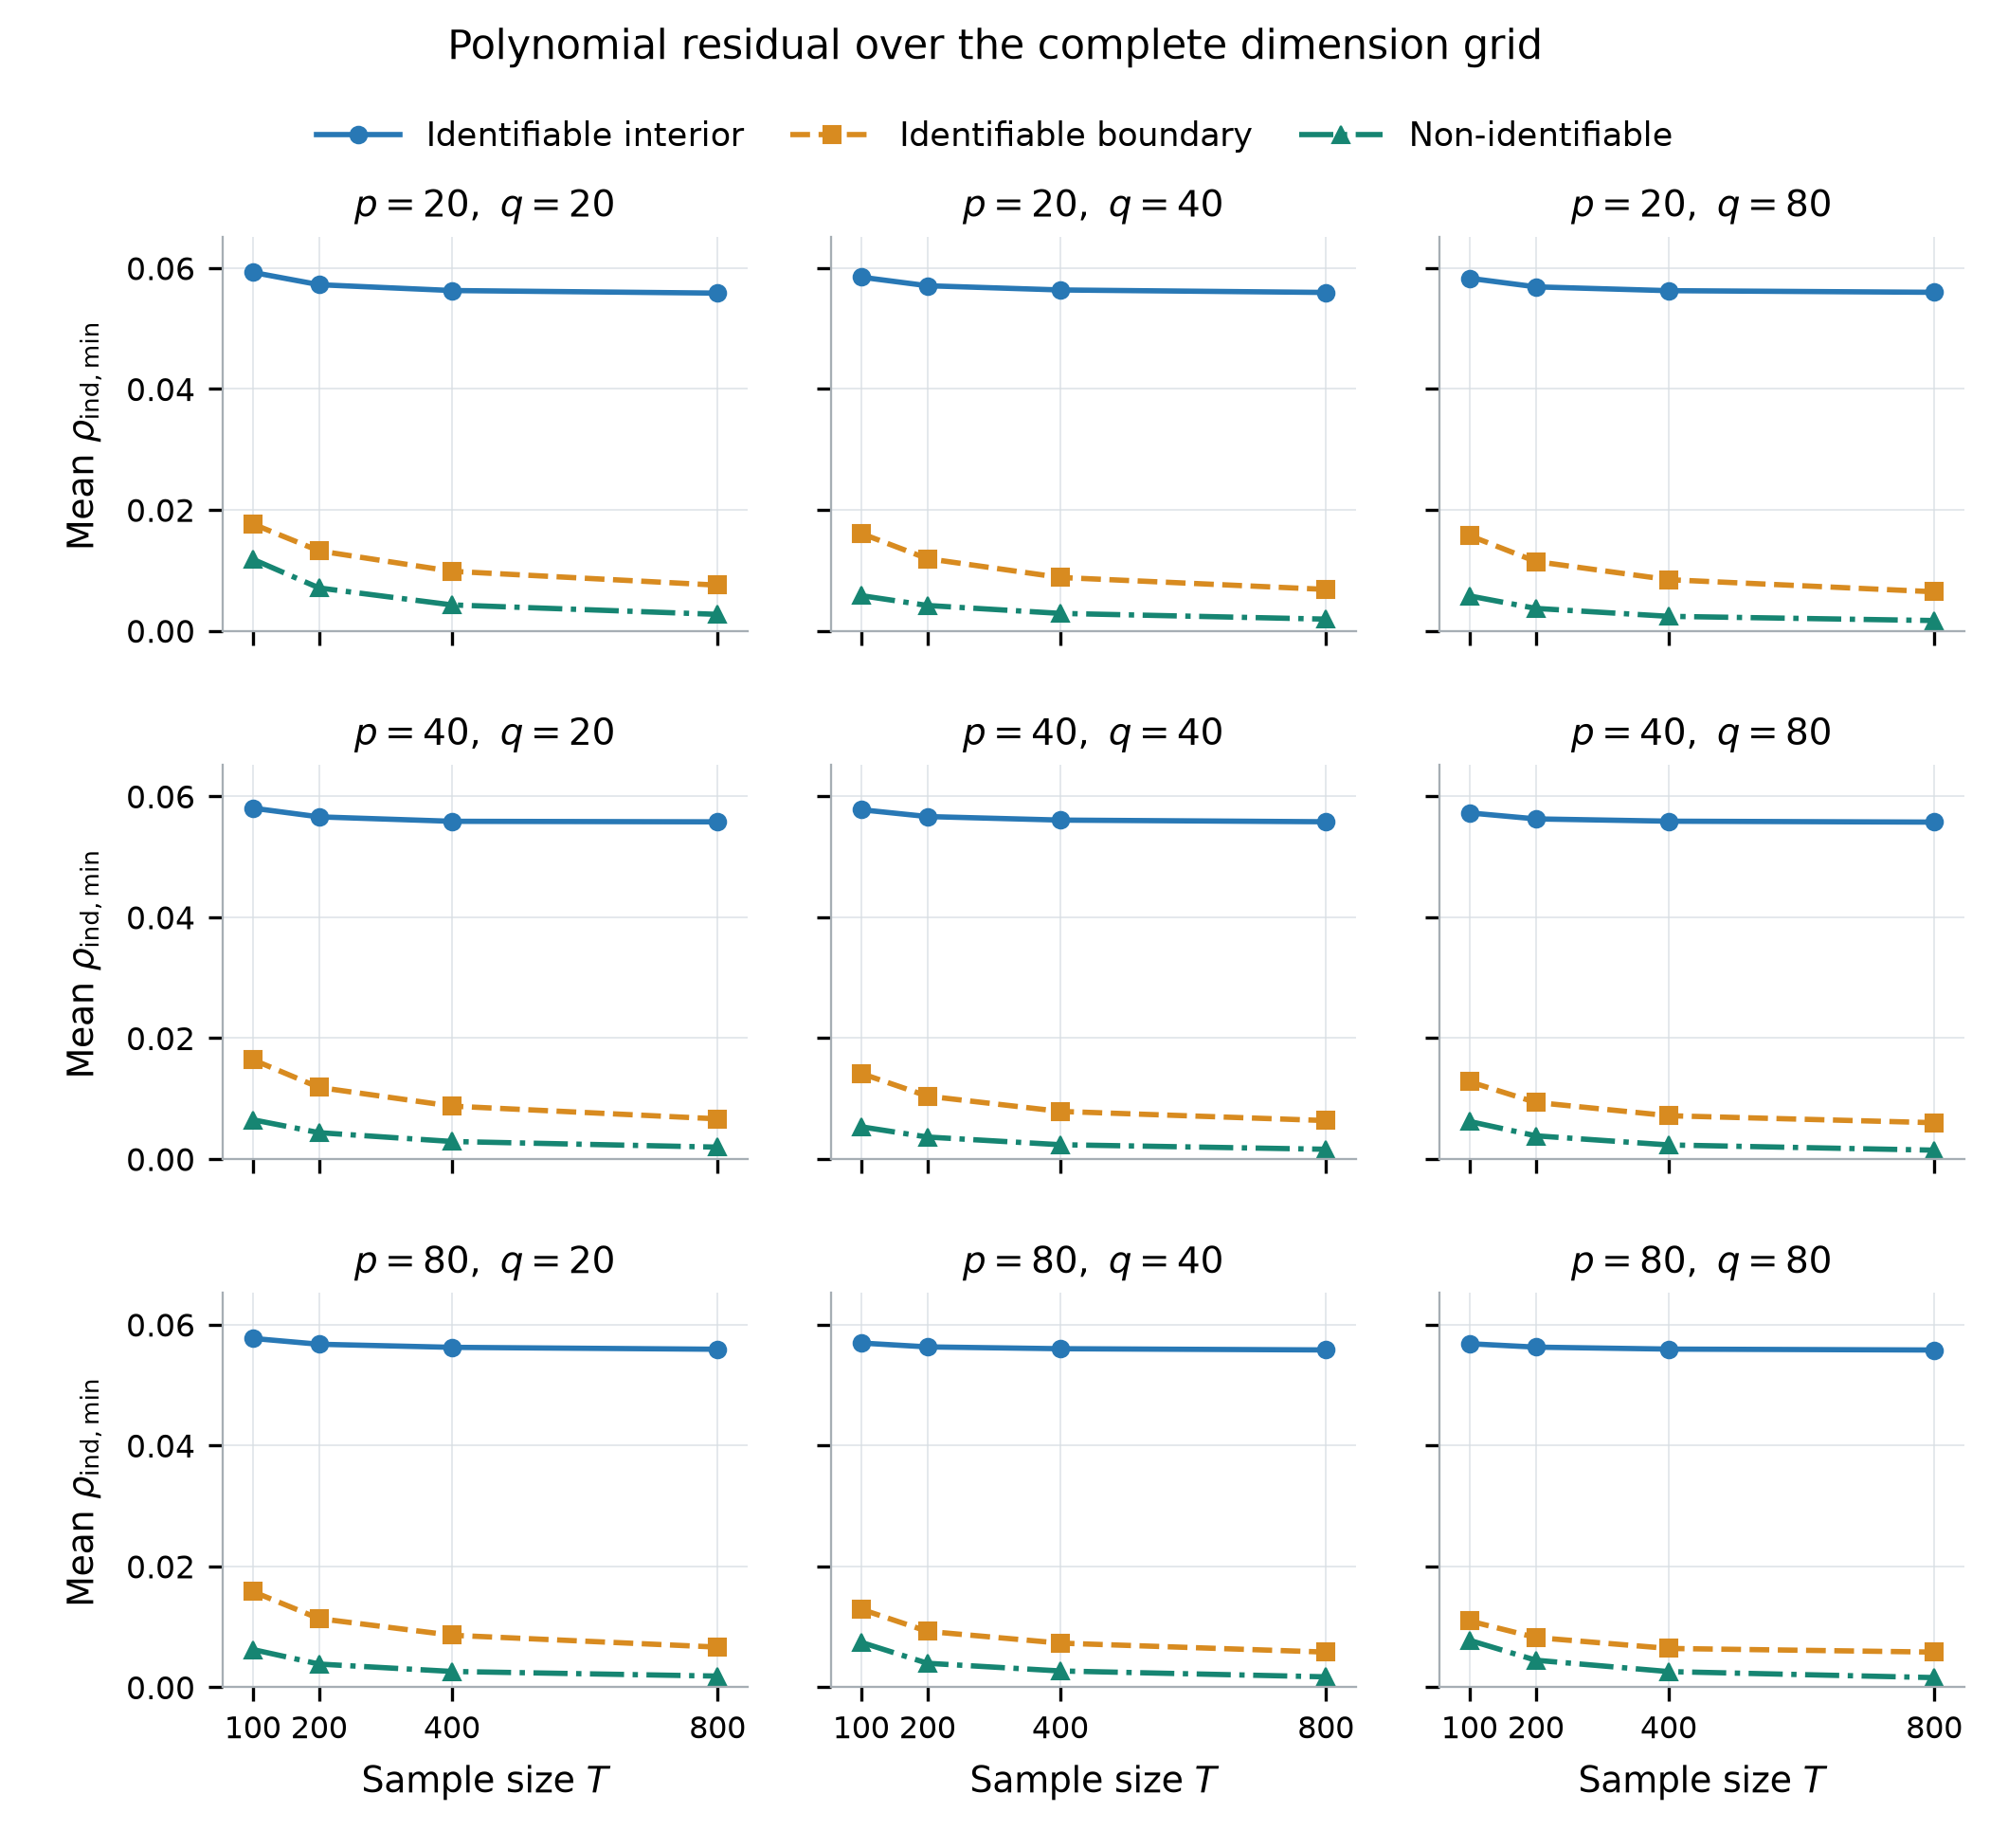
\includegraphics[width=0.98\linewidth,height=0.75\textheight,keepaspectratio]{images/lambda_grid_rho.png}
\caption{Lowest found polynomial ratio in the recomputed coefficient-angle experiment, over all nine ordered dimension pairs. Each panel fixes $(p,q)$ and shows the three regimes at $T=100,200,400,800$. The plotted ratio is $\rho_{\mathrm{ind}}=\rho/2$, using each independent minor once. Searches impose $\max_j|\lambda_j|/\|\lambda\|_2\le0.90$, so each direction is at least $\arccos(0.90)\approx25.84^\circ$ from every coordinate axis in the fitted unit-column basis. This is a fixed exclusion from the axes; the polynomial score alone does not detect an axis Jacobian singularity. Points are cell means (or detection fractions), without uncertainty bands; mean [sample variance] and actual denominators are tabulated separately. All cells have 100 estimates except the interior $80\times80$, $T=100$ cell, which has 96. Shared seed indices across cells do not form 900 independent replications. The axes are shared across panels within each figure.}
\label{s23:lambda:allfig:rho}
\endgroup
\end{figure}

\clearpage
\begin{figure}[p]
\begingroup
\spacingset{1.08}
\centering
\setkeys{Gin}{width=!,height=!}
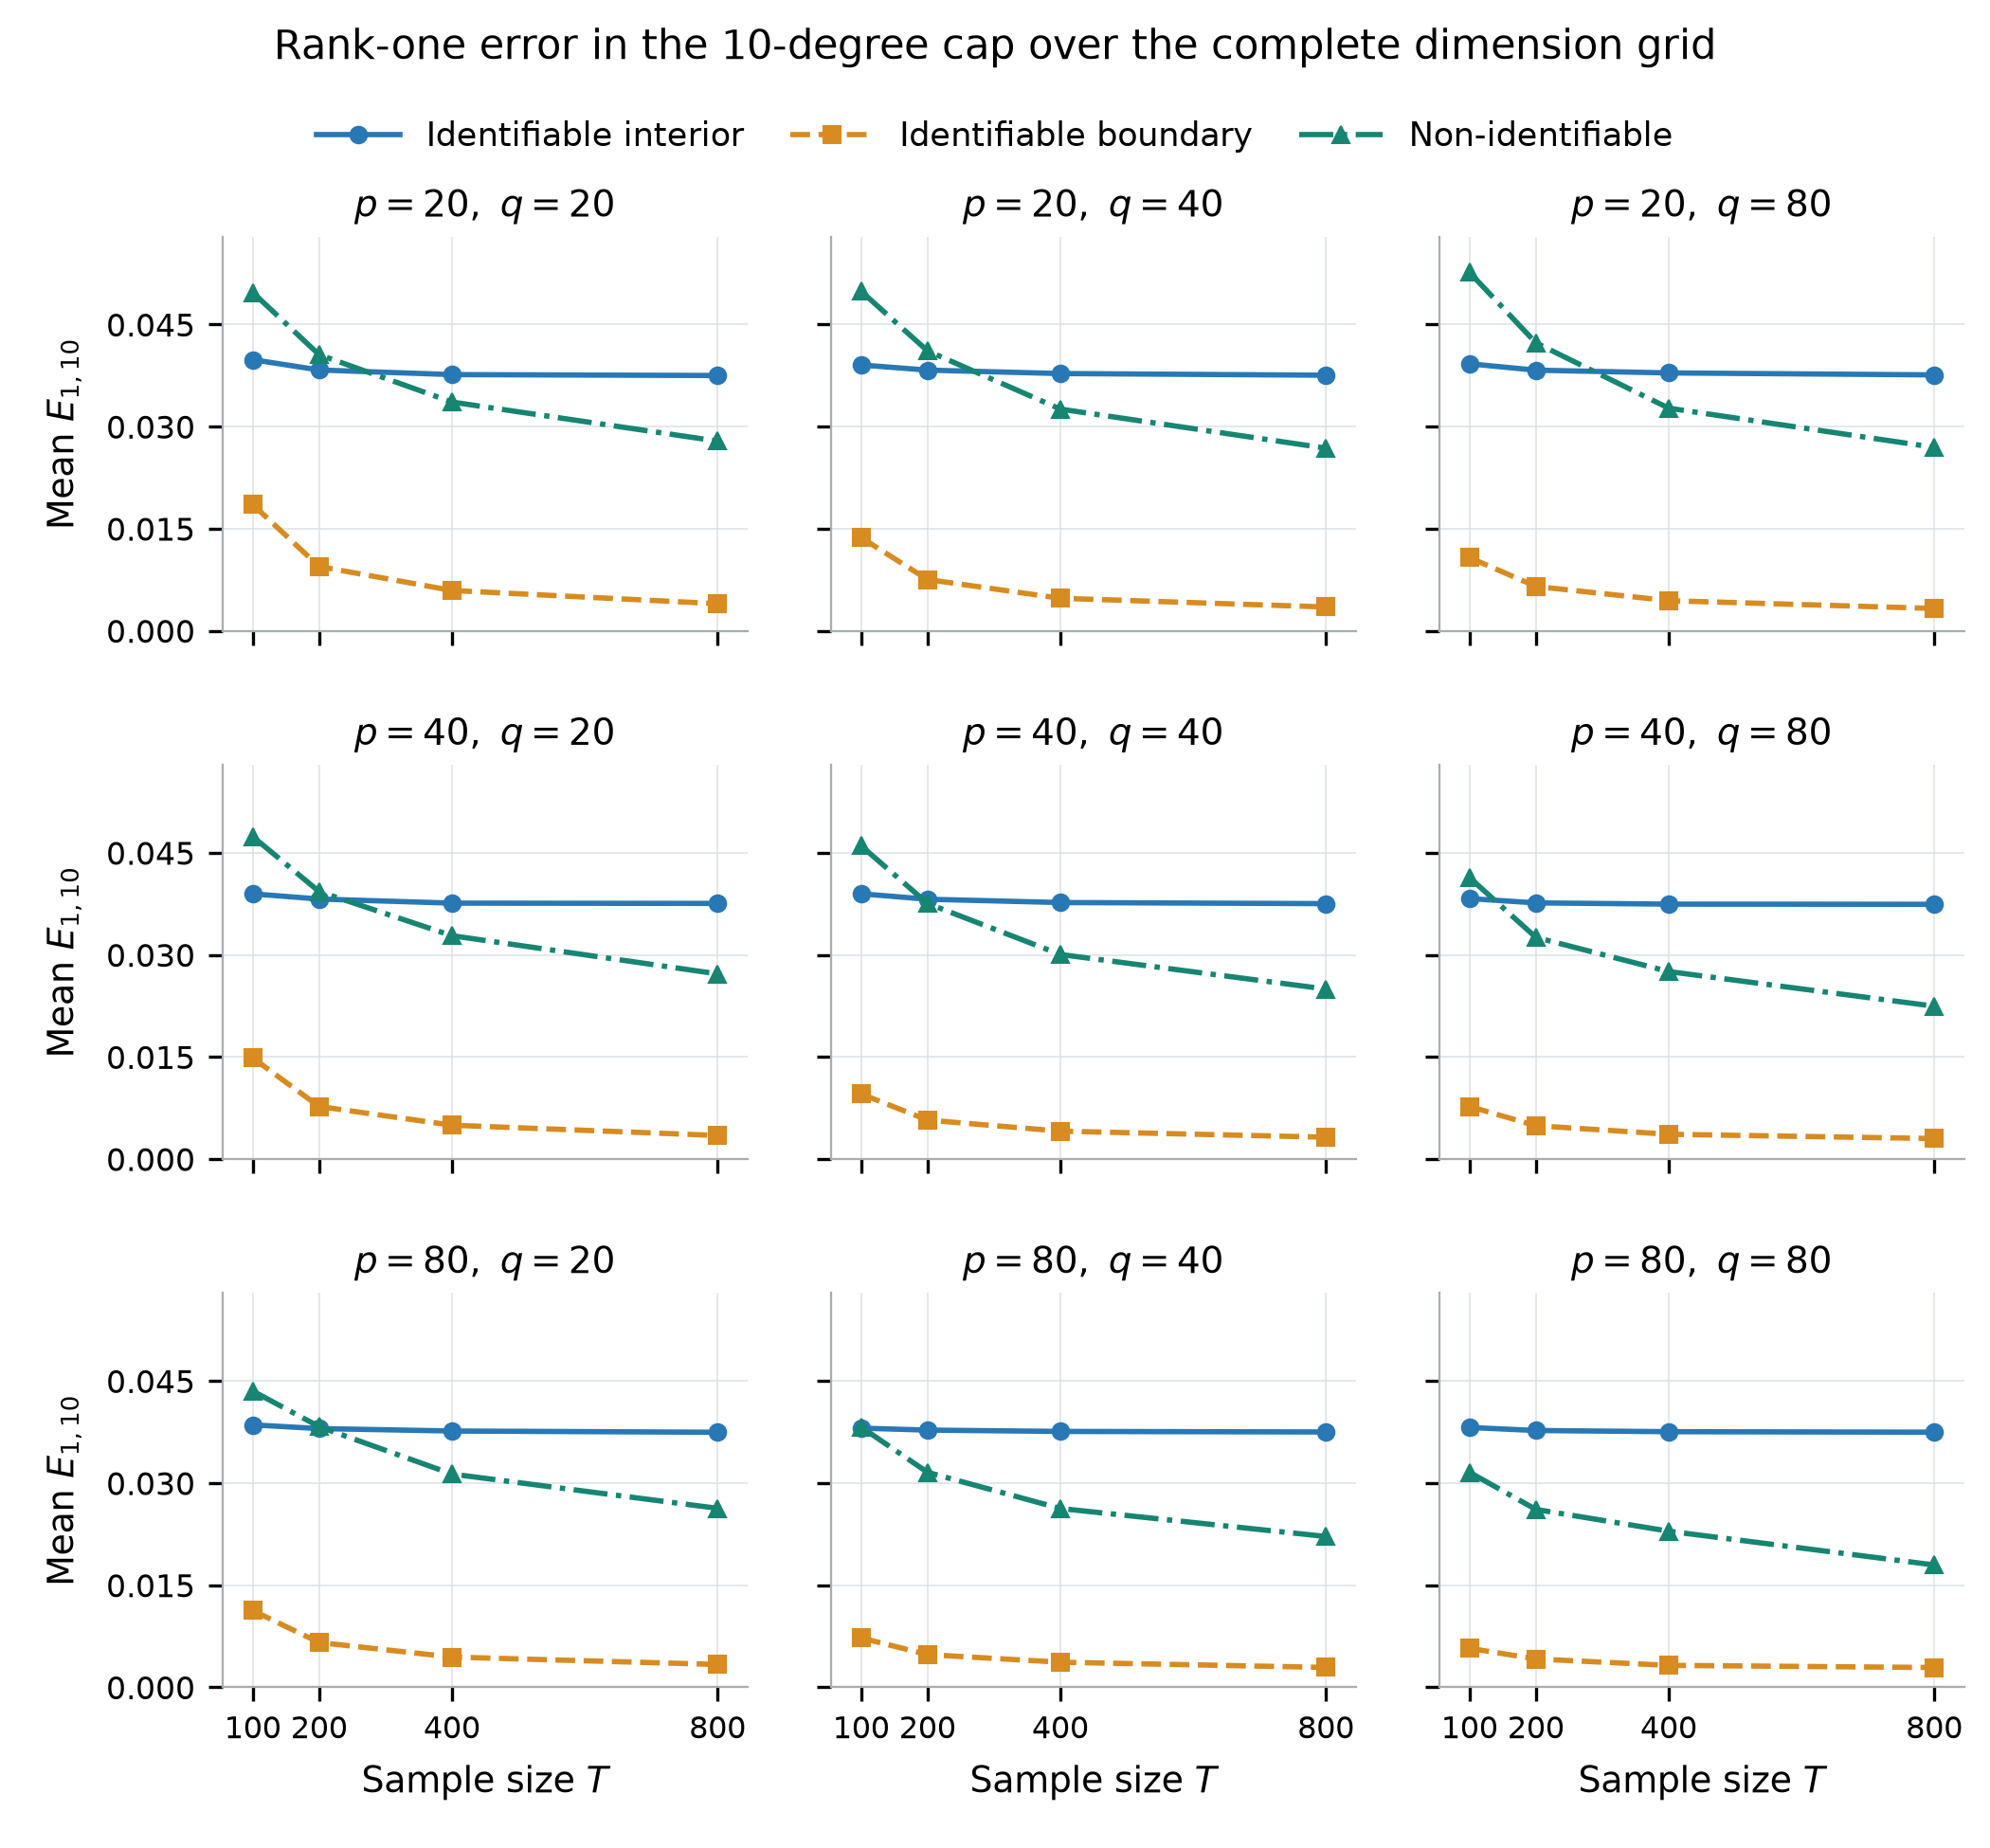
\includegraphics[width=0.98\linewidth,height=0.75\textheight,keepaspectratio]{images/lambda_grid_cap10.png}
\caption{Lowest found relative rank-one error within the $10^\circ$ projective coefficient-angle cap around the lowest $\rho_{\mathrm{ind}}$ candidate, for all nine ordered dimension pairs in the recomputed coefficient-angle experiment. The common exclusion is $\max_j|\lambda_j|/\|\lambda\|_2\le0.90$. The matrix cosine to an original loading is reported separately as an auxiliary quantity and is not constrained. Cap proximity is imposed, so a small cap residual and correspondence of independently searched local candidates have different interpretations. Points are cell means (or detection fractions), without uncertainty bands; mean [sample variance] and actual denominators are tabulated separately. All cells have 100 estimates except the interior $80\times80$, $T=100$ cell, which has 96. Shared seed indices across cells do not form 900 independent replications. The axes are shared across panels within each figure.}
\label{s23:lambda:allfig:cap10}
\endgroup
\end{figure}

\clearpage
\begin{figure}[p]
\begingroup
\spacingset{1.08}
\centering
\setkeys{Gin}{width=!,height=!}
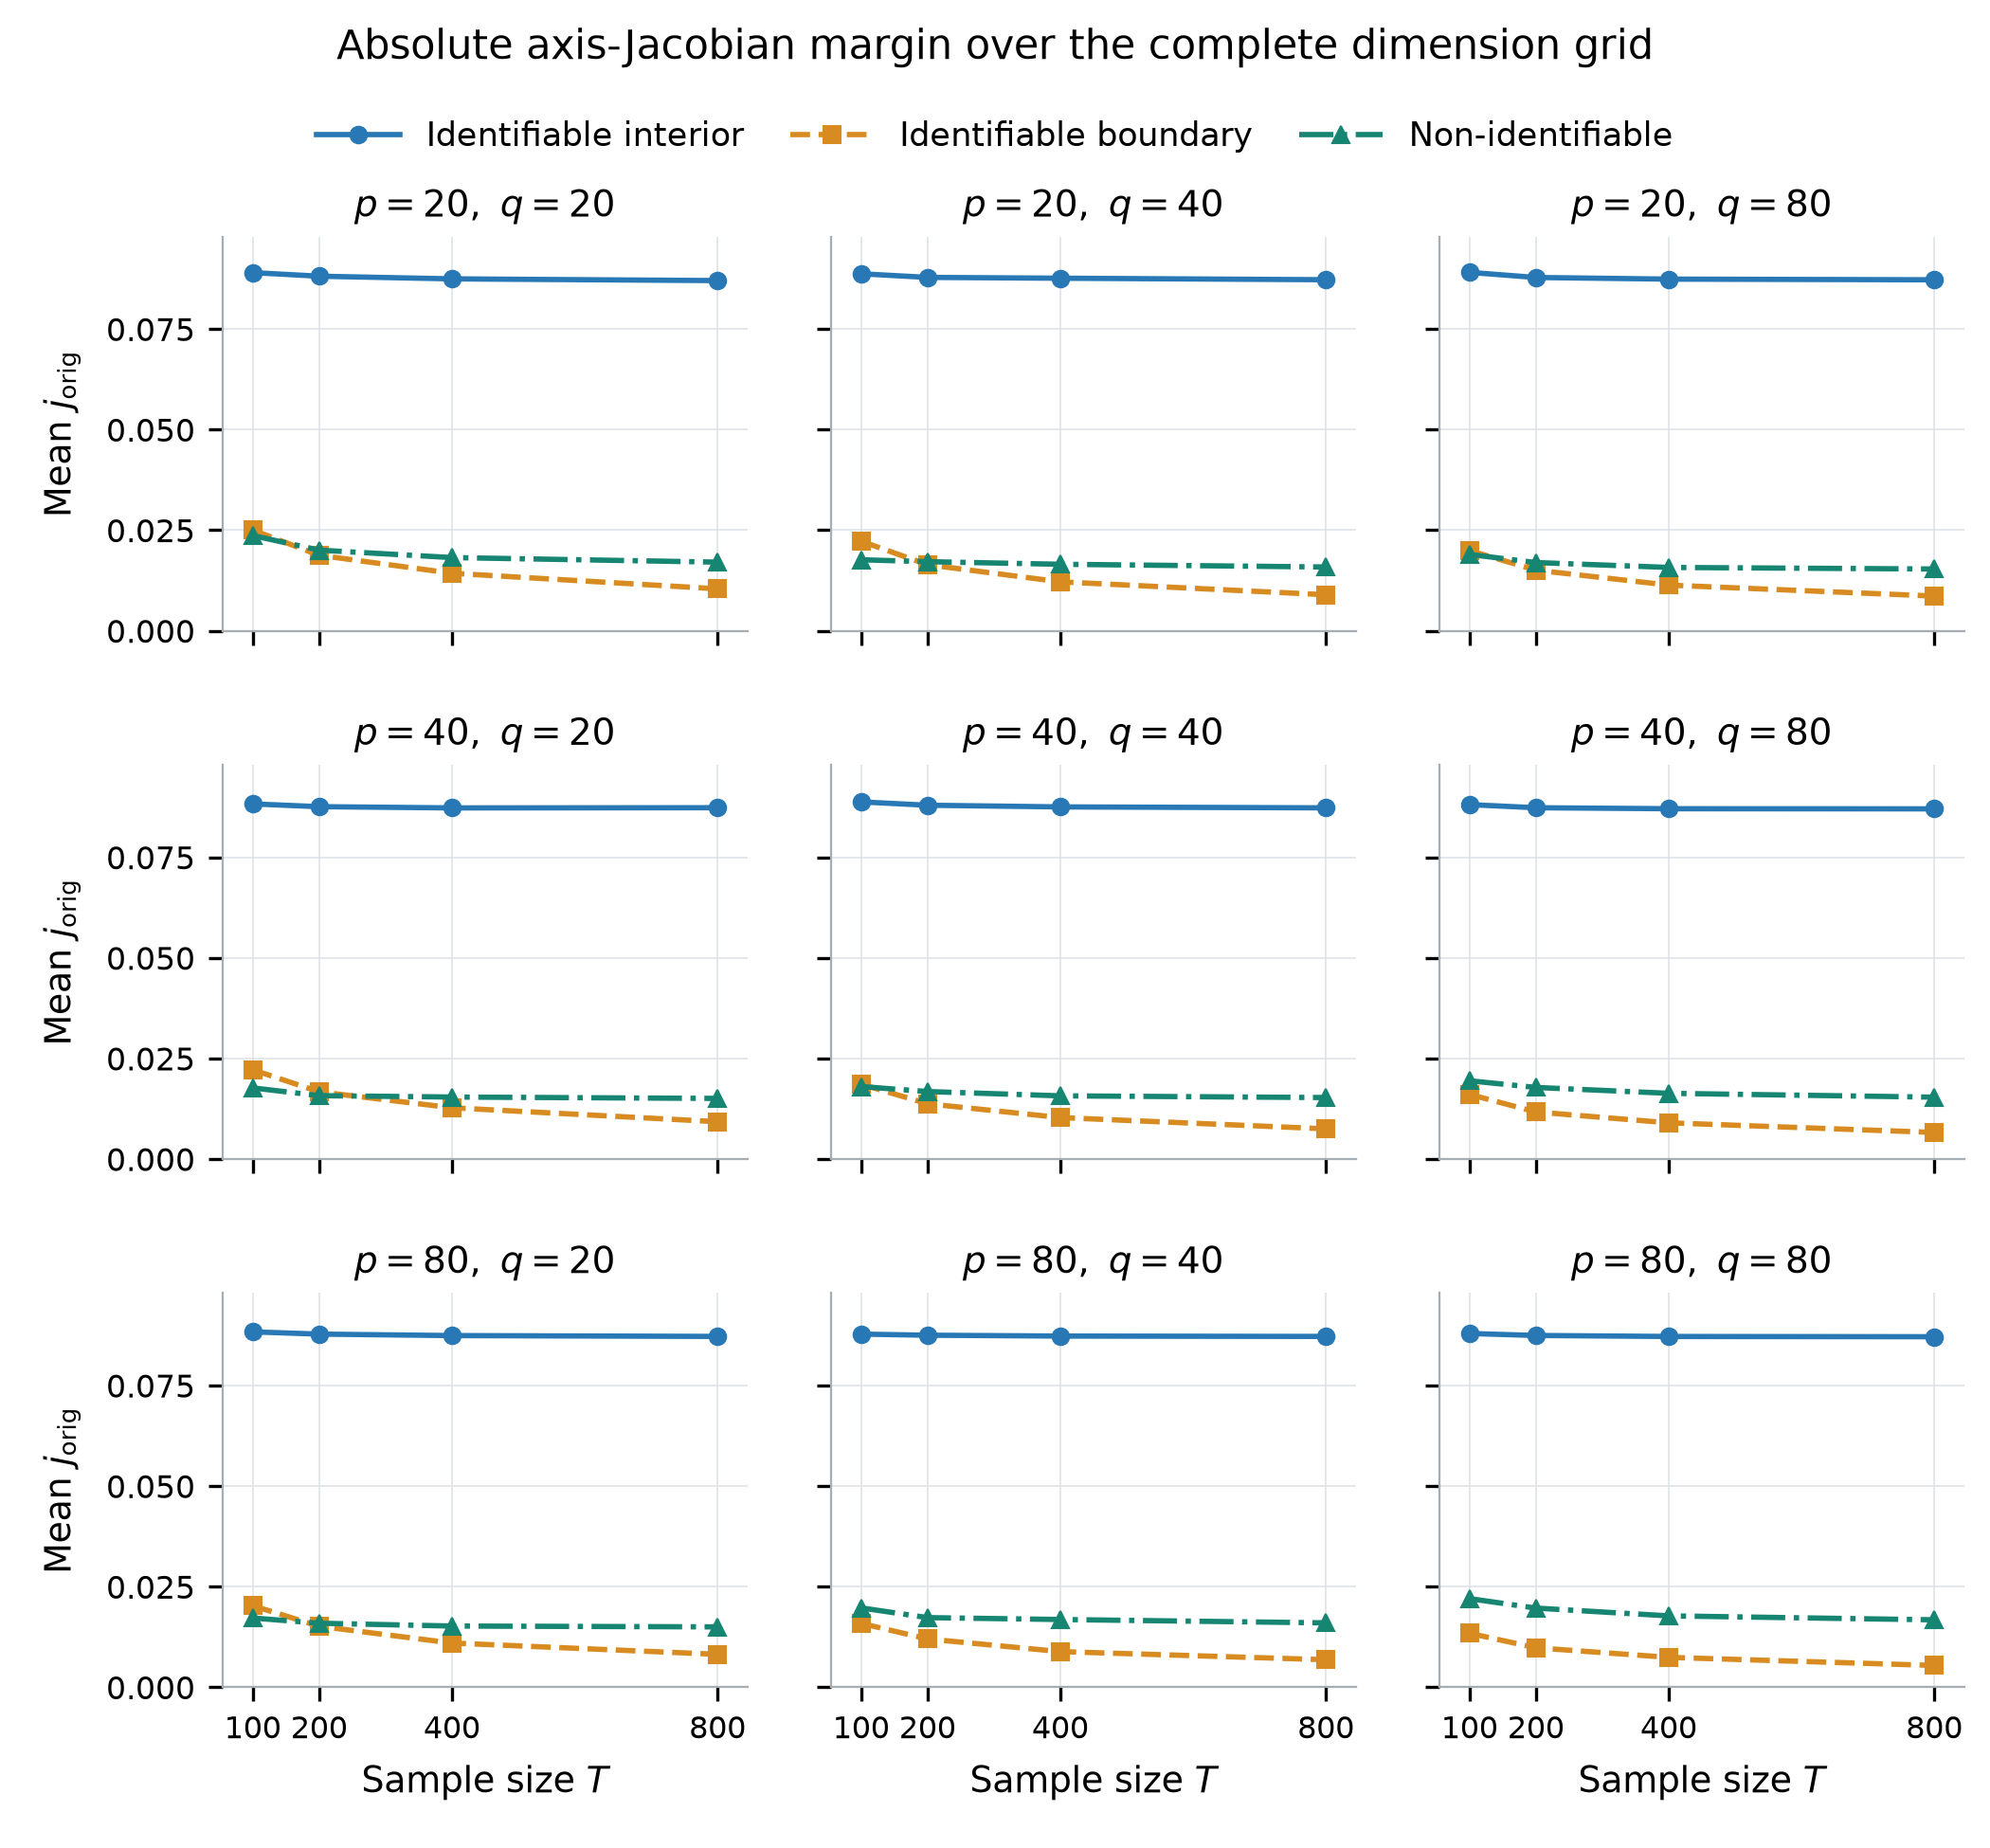
\includegraphics[width=0.98\linewidth,height=0.75\textheight,keepaspectratio]{images/lambda_grid_Jorig.png}
\caption{Absolute axis-Jacobian margin $j_{\mathrm{orig}}=\min_\ell s_{\ell,1}$ over all nine ordered dimension pairs. These singular values are unchanged by replacing the matrix-angle exclusion with the coefficient-angle exclusion: they depend only on the saved fitted loadings. Singular values are unsquared and use the $\psi$-column convention of the main article. Non-identifiable fits are retained across their alternative bases; a mixed-basis mean is not interpreted as a single-basis population reference. Points are cell means (or detection fractions), without uncertainty bands; mean [sample variance] and actual denominators are tabulated separately. All cells have 100 estimates except the interior $80\times80$, $T=100$ cell, which has 96. Shared seed indices across cells do not form 900 independent replications. The axes are shared across panels within each figure.}
\label{s23:lambda:allfig:Jorig}
\endgroup
\end{figure}

\clearpage
\begin{figure}[p]
\begingroup
\spacingset{1.08}
\centering
\setkeys{Gin}{width=!,height=!}
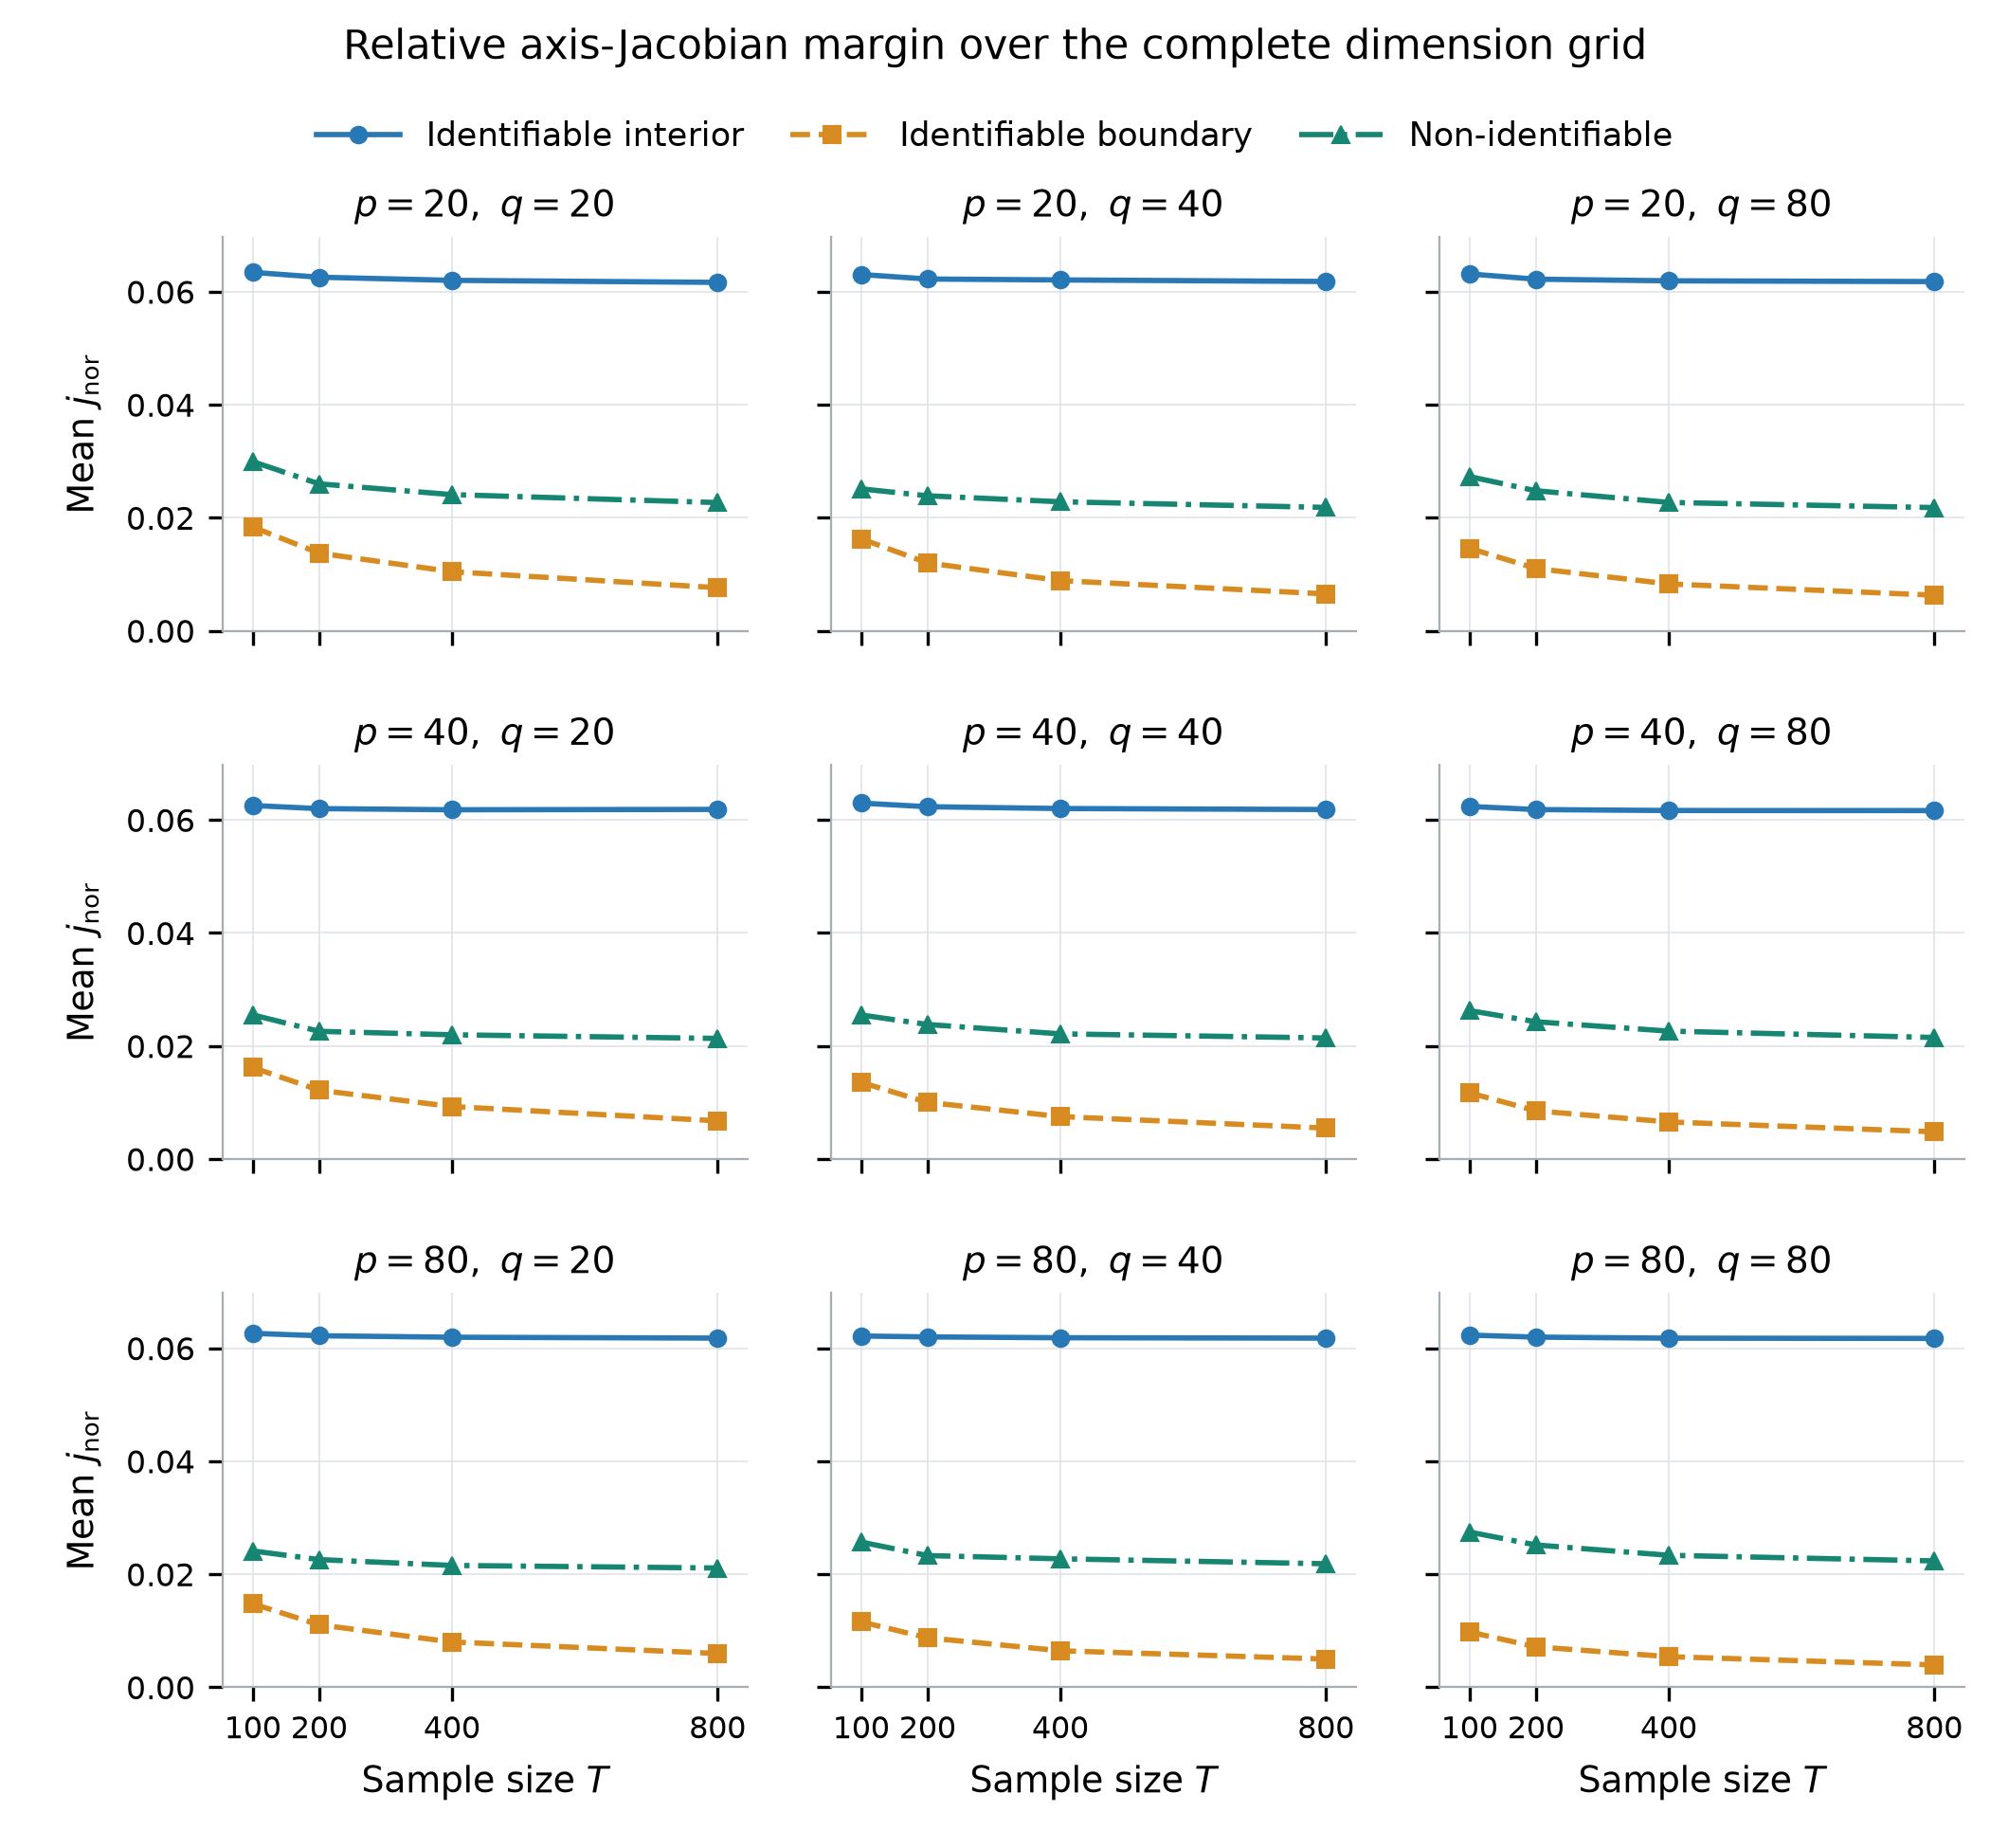
\includegraphics[width=0.98\linewidth,height=0.75\textheight,keepaspectratio]{images/lambda_grid_Jnor.png}
\caption{Relative axis-Jacobian margin $j_{\mathrm{nor}}=\min_\ell s_{\ell,1}/s_{\ell,d-1}$ over all nine ordered dimension pairs. These fitted-loading spectra are unchanged by the new coefficient-angle exclusion. Each Jacobian is normalized within each seed before taking the mean. This unsquared ratio is distinct from the $s_{\ell,2}/s_{\ell,1}$ spectral gap used in the real-data table. Points are cell means (or detection fractions), without uncertainty bands; mean [sample variance] and actual denominators are tabulated separately. All cells have 100 estimates except the interior $80\times80$, $T=100$ cell, which has 96. Shared seed indices across cells do not form 900 independent replications. The axes are shared across panels within each figure.}
\label{s23:lambda:allfig:Jnor}
\endgroup
\end{figure}

\clearpage
\begin{figure}[p]
\begingroup
\spacingset{1.08}
\centering
\setkeys{Gin}{width=!,height=!}
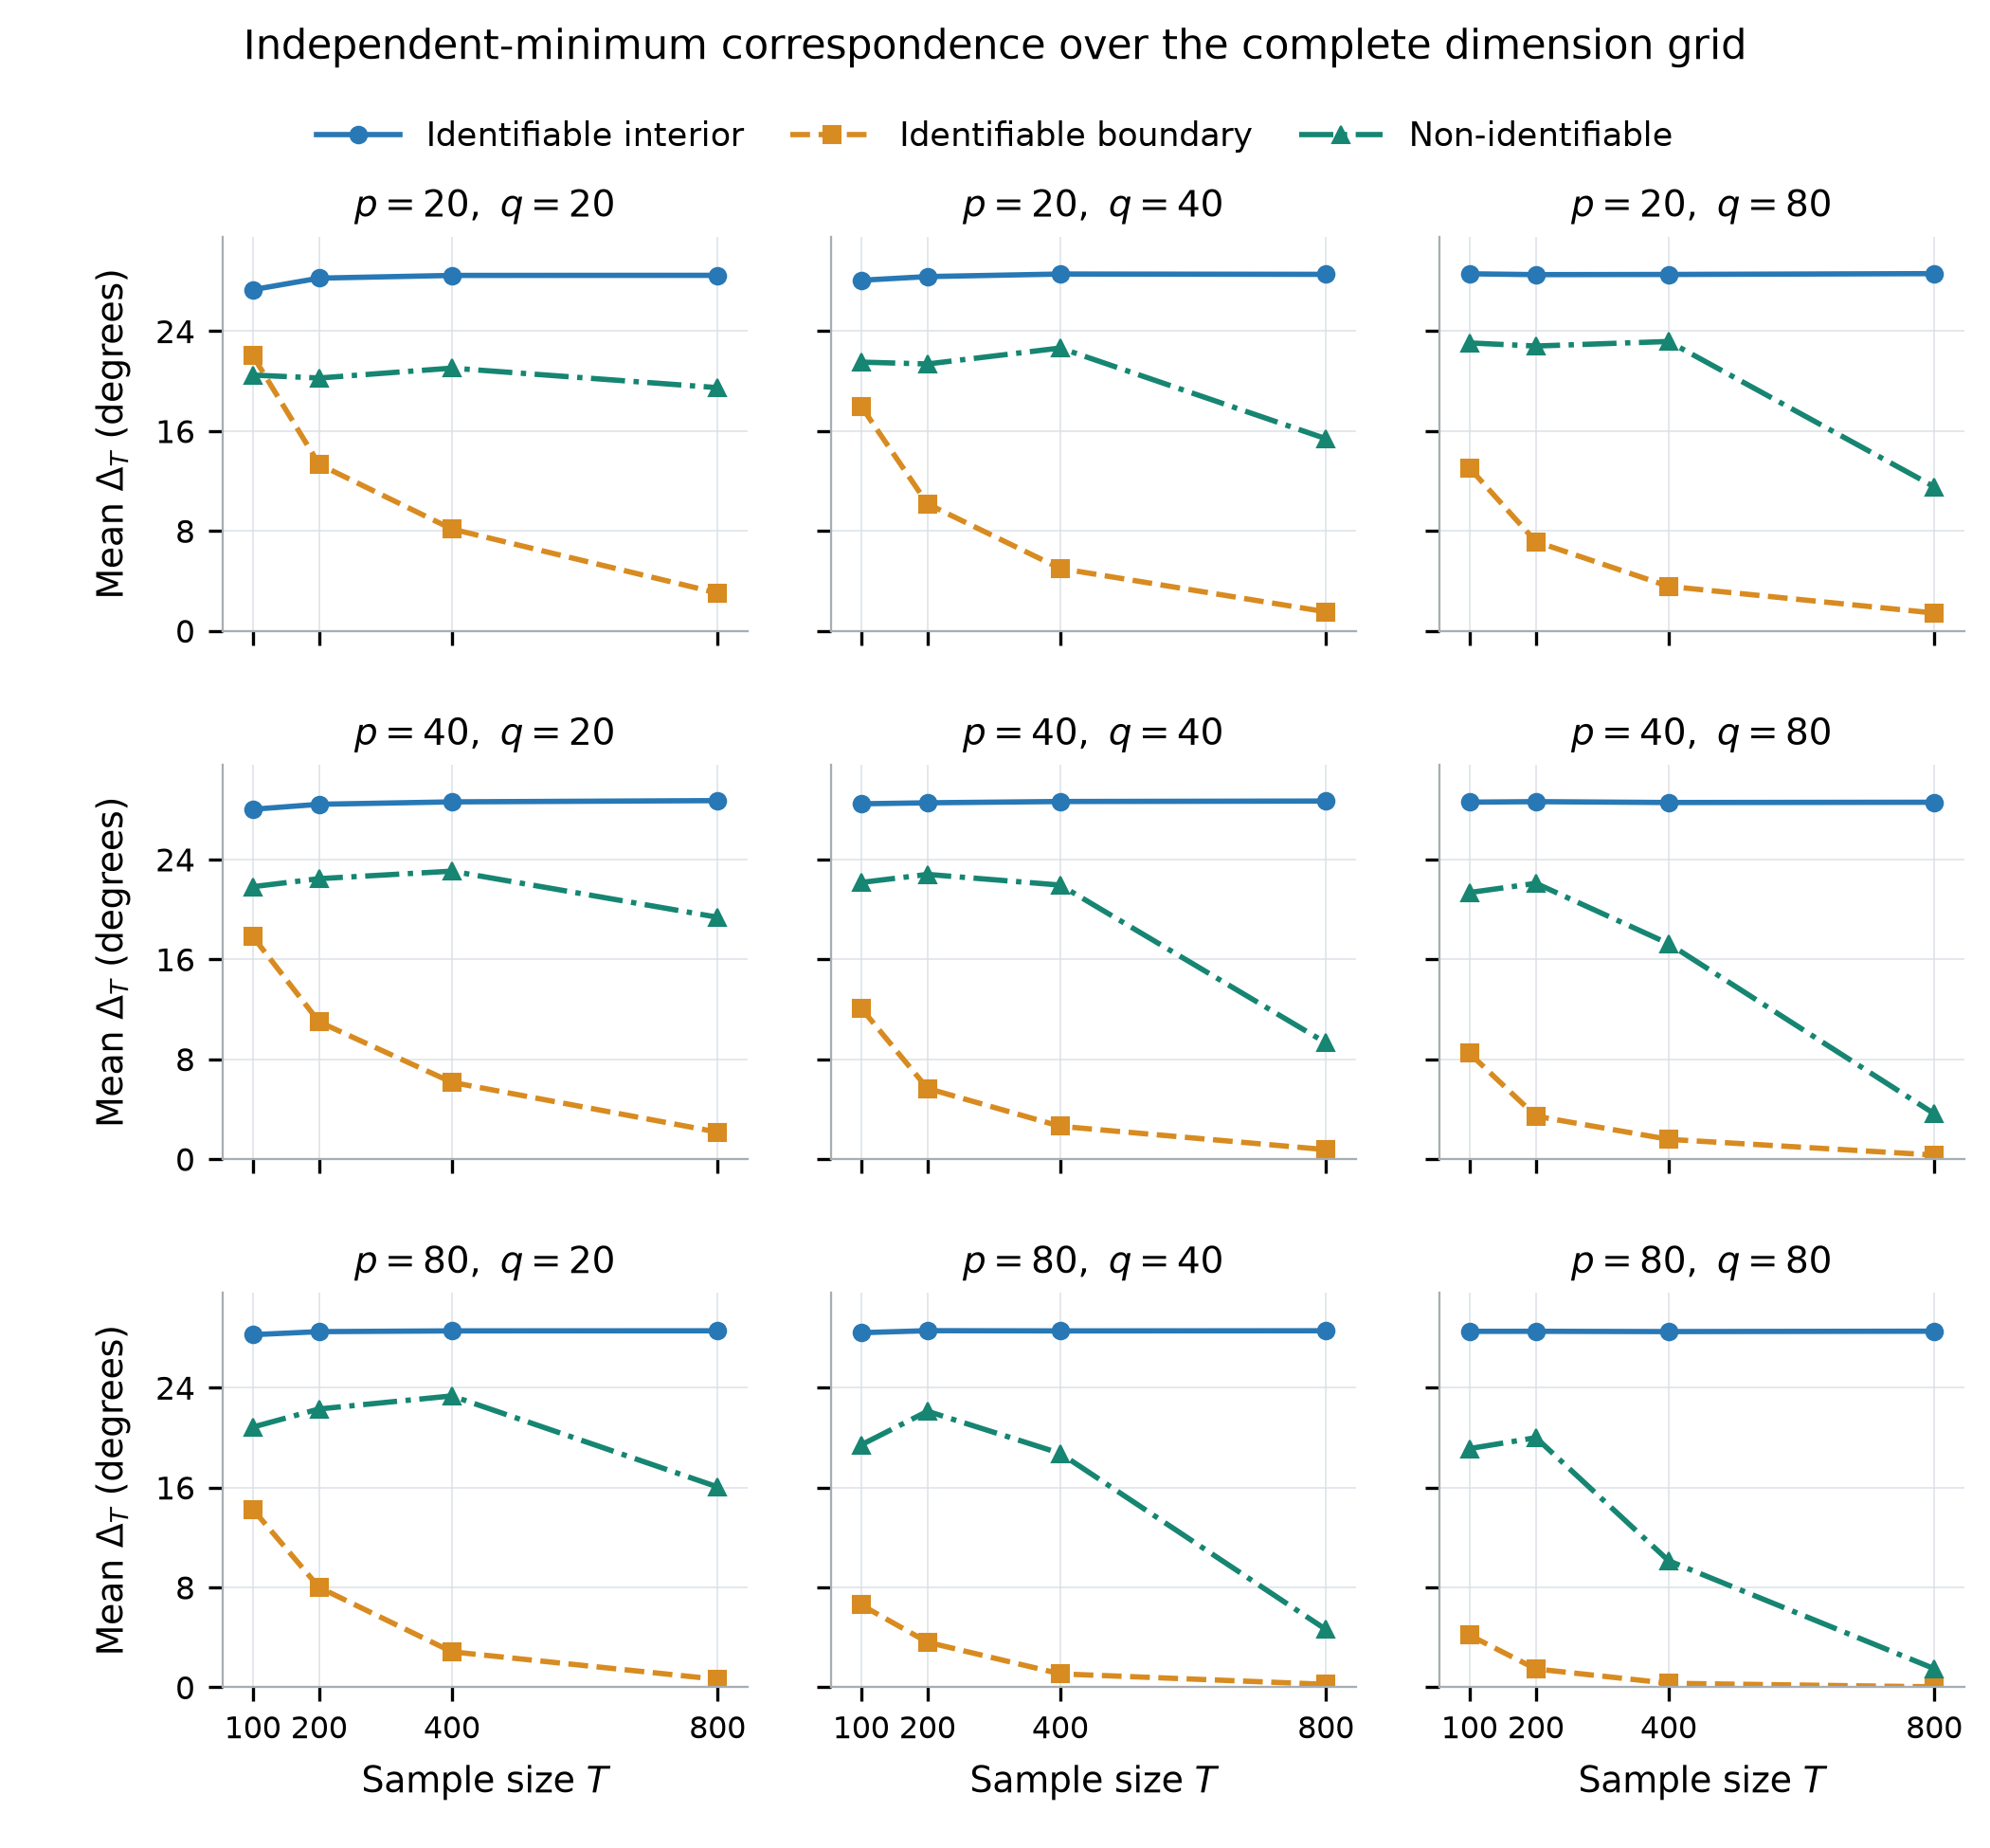
\includegraphics[width=0.98\linewidth,height=0.75\textheight,keepaspectratio]{images/lambda_grid_angle.png}
\caption{Projective coefficient angle $\Delta_T$ from the lowest $\rho_{\mathrm{ind}}$ candidate to its nearest independently searched $E_1$ candidate, within the same fitted unit-column basis and the common exclusion $\max_j|\lambda_j|/\|\lambda\|_2\le0.90$. This is distinct from the automatically bounded angle to a cap solution. The full observed range of cell means is shown; proximity of positive minima alone does not identify a common zero. Points are cell means (or detection fractions), without uncertainty bands; mean [sample variance] and actual denominators are tabulated separately. All cells have 100 estimates except the interior $80\times80$, $T=100$ cell, which has 96. Shared seed indices across cells do not form 900 independent replications. The axes are shared across panels within each figure.}
\label{s23:lambda:allfig:angle}
\endgroup
\end{figure}

\clearpage
\begin{figure}[p]
\begingroup
\spacingset{1.08}
\centering
\setkeys{Gin}{width=!,height=!}
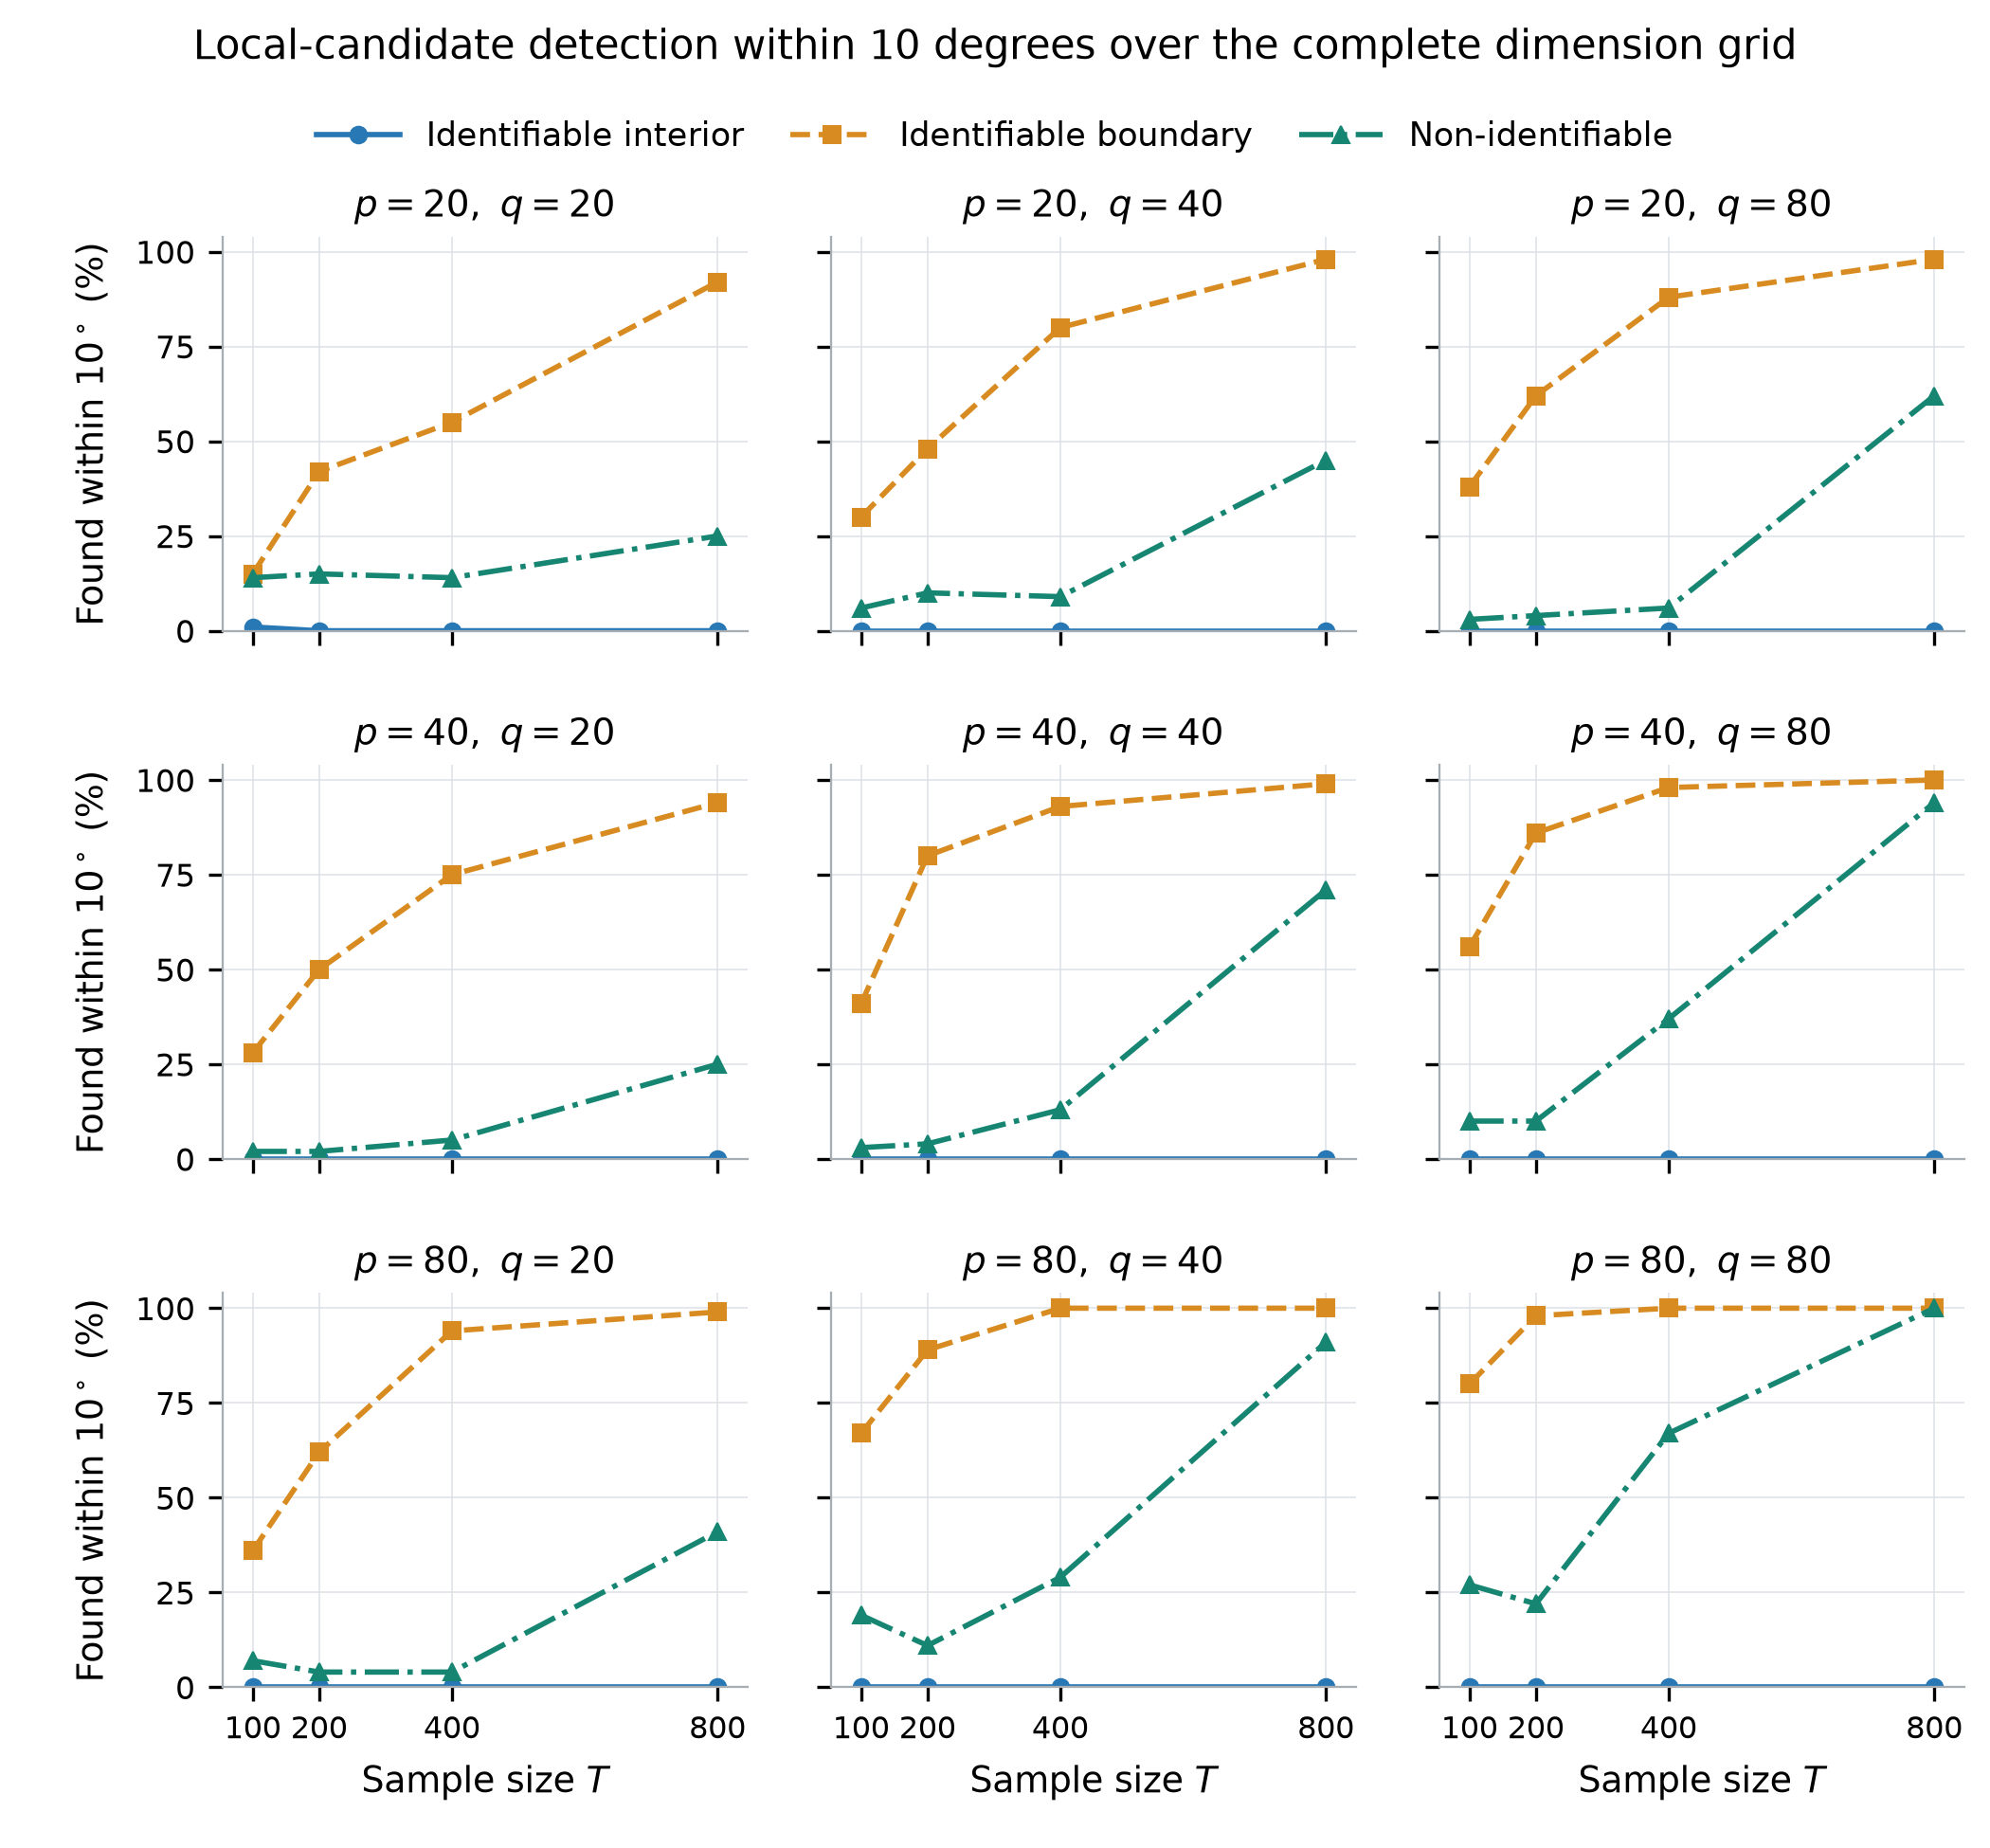
\includegraphics[width=0.98\linewidth,height=0.75\textheight,keepaspectratio]{images/lambda_grid_localrate.png}
\caption{Fraction of estimates with a found local $E_1$ candidate within a $10^\circ$ projective coefficient angle of the lowest $\rho_{\mathrm{ind}}$ center, under the coefficient-axis exclusion $\max_j|\lambda_j|/\|\lambda\|_2\le0.90$. An eligible candidate is a successful saved independent candidate there or a successful feasible refinement that remains there after removing only the angular-cap constraint. The fixed coordinate-axis exclusion remains active. The denominator includes every available estimate, and no missing candidate is imputed as a zero residual. Numerical success is not an analytic local-optimality certificate. Points are cell means (or detection fractions), without uncertainty bands; mean [sample variance] and actual denominators are tabulated separately. All cells have 100 estimates except the interior $80\times80$, $T=100$ cell, which has 96. Shared seed indices across cells do not form 900 independent replications. The axes are shared across panels within each figure.}
\label{s23:lambda:allfig:localrate}
\endgroup
\end{figure}

\clearpage
\begin{figure}[p]
\begingroup
\spacingset{1.08}
\centering
\setkeys{Gin}{width=!,height=!}
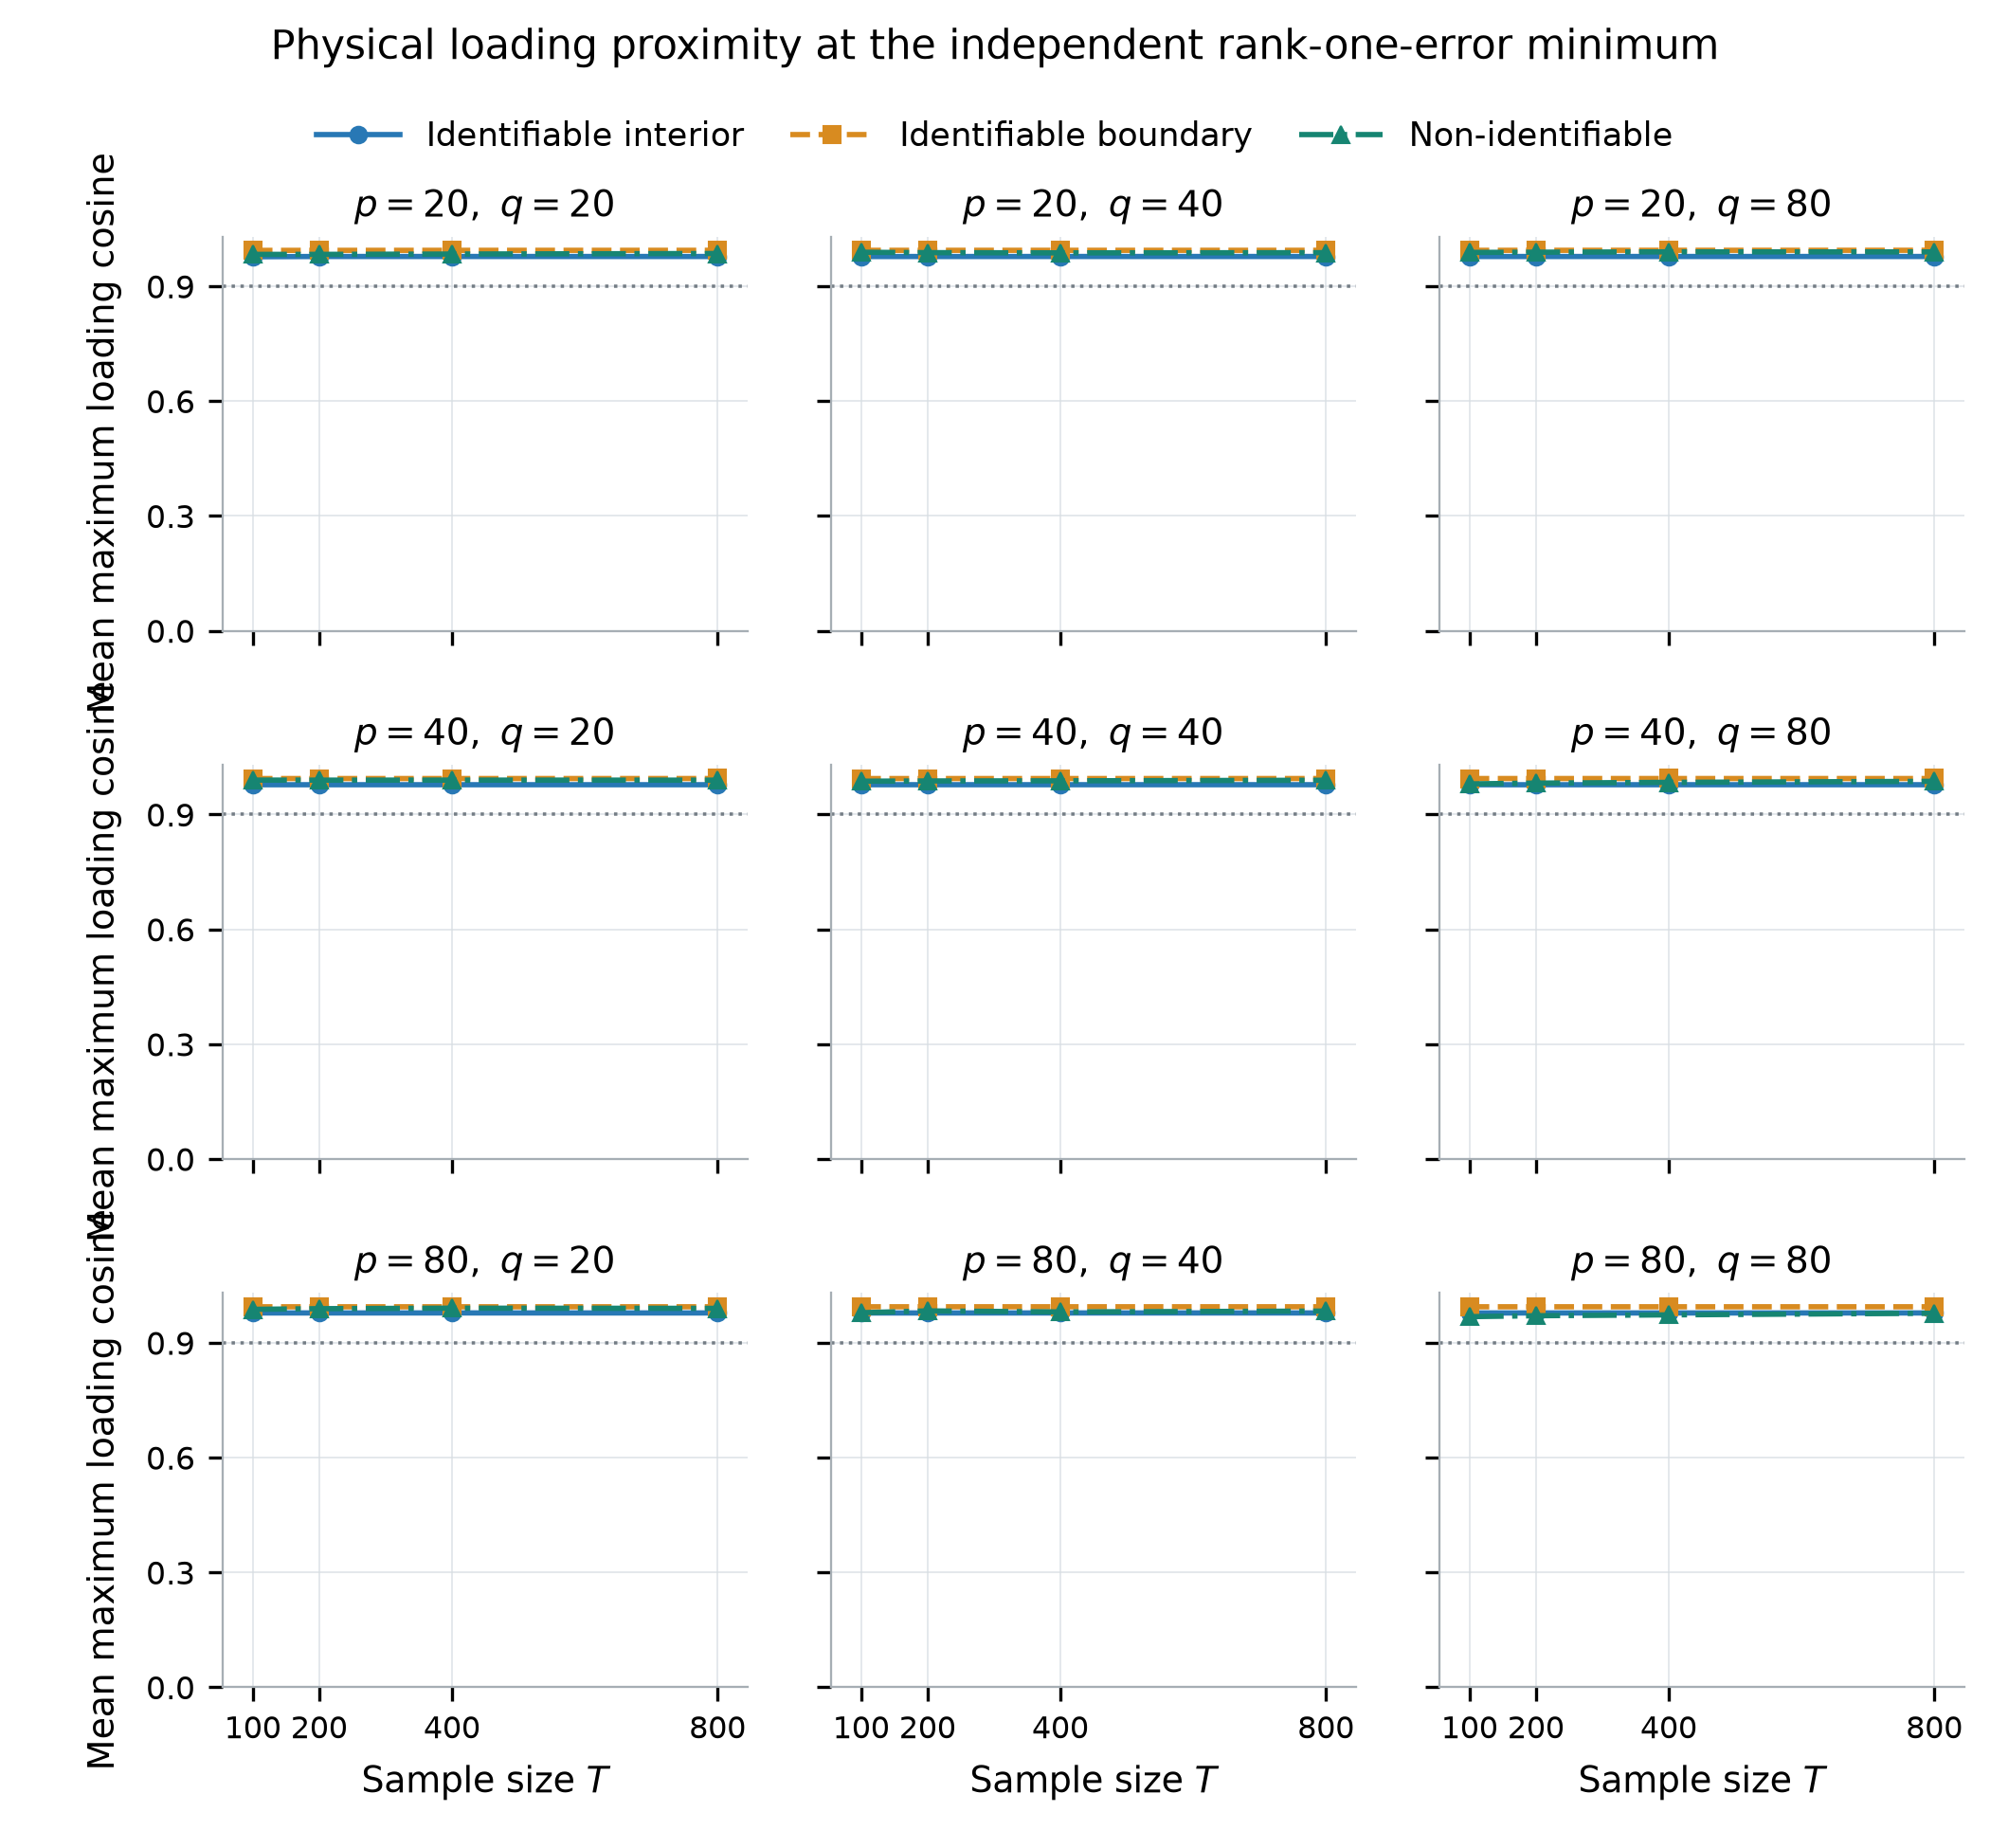
\includegraphics[width=0.98\linewidth,height=0.75\textheight,keepaspectratio]{images/lambda_grid_physicalcos.png}
\caption{Mean maximum absolute Frobenius cosine between the independently selected $E_1$-minimum matrix and the fitted original rank-one loadings, in the recomputed coefficient-angle experiment. This is an auxiliary physical-space proximity measure: it is not constrained by the new coefficient-axis exclusion. The dotted line at $0.90$ is the exclusion threshold used by the archived matrix-angle experiment, shown only for comparison. The full interval from zero to one is displayed, so no cell means are hidden by a zoom. A direction far from the coefficient axes can still produce a matrix close to an original loading when the loading atoms are correlated. Points are cell means (or detection fractions), without uncertainty bands; mean [sample variance] and actual denominators are tabulated separately. All cells have 100 estimates except the interior $80\times80$, $T=100$ cell, which has 96. Shared seed indices across cells do not form 900 independent replications. The axes are shared across panels within each figure.}
\label{s23:lambda:allfig:physicalcos}
\endgroup
\end{figure}

\clearpage

\FloatBarrier
\clearpage
\section{Archived matrix-angle comparisons}
\clearpage
\paragraph{Archived matrix-angle comparison and its computational audits.}
The following four tables and two figures retain selected results
from the earlier domain $\mathcal D^M_{0.90}$, where separation
from the original loading matrices was imposed directly. They are
labelled as archived matrix-angle results and are not included in
the new coefficient-angle summaries or AUCs.
For example, at $40\times40$, $T=800$, boundary mean $E_{1,10}$
is $0.052419$ on the archived matrix-angle domain, versus
$0.003203$ on the new coefficient-angle domain. The corresponding
independent minimum moves from a physically separated valley to a
combination with physical cosine near $0.994$. The feasible sets
differ, so neither numerical ordering nor local-candidate counts
can be transferred between them. Their QMLE fits and Jacobian
spectra are identical.

The archived computation increased cap searches to 20 starts and
600 evaluations on 216 purposively selected fits; none of its
54 $T=800$ cases improved by more than $10^{-7}$. Its selected
continuation audit also examined the $5^\circ$ and $10^\circ$
scores after additional QMLE optimization, as shown in
Table~\ref{s23:tab:cap_iteration}. These are checks of the archived
matrix-angle calculation. They do not establish robustness of the
new coefficient-angle searches, and no $0.95$ matrix-cutoff result
is described as a sensitivity analysis of the new axis-angle rule.

% Adapted from the independently validated diagnostic tables; numeric entries unchanged.
% Sources: final_summary_20261030 key tables, cap10_supplement_20261030/tables,
% and final_summary_20261030/iteration_cap10_audit.
% Every bracket is a sample variance (denominator n-1), not an SD.
% Singular values and E1 are unsquared, without multiplication by 100.
\begin{table}[p]
\begingroup
\spacingset{1.08}
\centering
\caption{Archived matrix-angle experiment: Rank-one errors at the lowest found $\rho_{\mathrm{ind}}$ candidate and in its angular neighborhoods, $p=q=40$. Each entry is mean [sample variance] over all 100 seeds.}
\label{s23:tab:cap_comparison}
\small
\setlength{\tabcolsep}{6pt}
\renewcommand{\arraystretch}{1.10}
\begin{adjustbox}{max width=\linewidth}
\begin{tabular}{lrccc}
\toprule
Design & $T$ & $E_{1,\mathrm{center}}$ & $E_{1,5}$ & $E_{1,10}$\\
\midrule
Interior & 100 & \shortstack{$0.04404$\\{\scriptsize$[5.26\times10^{-6}]$}} & \shortstack{$0.04100$\\{\scriptsize$[3.97\times10^{-6}]$}} & \shortstack{$0.04044$\\{\scriptsize$[3.11\times10^{-6}]$}}\\
Interior & 200 & \shortstack{$0.04307$\\{\scriptsize$[2.32\times10^{-6}]$}} & \shortstack{$0.04011$\\{\scriptsize$[1.82\times10^{-6}]$}} & \shortstack{$0.03965$\\{\scriptsize$[1.4\times10^{-6}]$}}\\
Interior & 400 & \shortstack{$0.04251$\\{\scriptsize$[8.85\times10^{-7}]$}} & \shortstack{$0.03959$\\{\scriptsize$[6.92\times10^{-7}]$}} & \shortstack{$0.03919$\\{\scriptsize$[5.7\times10^{-7}]$}}\\
Interior & 800 & \shortstack{$0.04229$\\{\scriptsize$[5.91\times10^{-7}]$}} & \shortstack{$0.03941$\\{\scriptsize$[4.61\times10^{-7}]$}} & \shortstack{$0.03902$\\{\scriptsize$[3.6\times10^{-7}]$}}\\
\addlinespace
Boundary & 100 & \shortstack{$0.05223$\\{\scriptsize$[6.16\times10^{-5}]$}} & \shortstack{$0.05213$\\{\scriptsize$[6.11\times10^{-5}]$}} & \shortstack{$0.05213$\\{\scriptsize$[6.11\times10^{-5}]$}}\\
Boundary & 200 & \shortstack{$0.05067$\\{\scriptsize$[4.02\times10^{-5}]$}} & \shortstack{$0.05058$\\{\scriptsize$[3.98\times10^{-5}]$}} & \shortstack{$0.05058$\\{\scriptsize$[3.98\times10^{-5}]$}}\\
Boundary & 400 & \shortstack{$0.05109$\\{\scriptsize$[3.58\times10^{-5}]$}} & \shortstack{$0.05101$\\{\scriptsize$[3.54\times10^{-5}]$}} & \shortstack{$0.05101$\\{\scriptsize$[3.54\times10^{-5}]$}}\\
Boundary & 800 & \shortstack{$0.05251$\\{\scriptsize$[2.43\times10^{-5}]$}} & \shortstack{$0.05242$\\{\scriptsize$[2.41\times10^{-5}]$}} & \shortstack{$0.05242$\\{\scriptsize$[2.41\times10^{-5}]$}}\\
\addlinespace
Exterior & 100 & \shortstack{$0.09127$\\{\scriptsize$[6.36\times10^{-4}]$}} & \shortstack{$0.06675$\\{\scriptsize$[3.22\times10^{-4}]$}} & \shortstack{$0.04588$\\{\scriptsize$[1.31\times10^{-4}]$}}\\
Exterior & 200 & \shortstack{$0.06311$\\{\scriptsize$[2.93\times10^{-4}]$}} & \shortstack{$0.04764$\\{\scriptsize$[1.6\times10^{-4}]$}} & \shortstack{$0.03752$\\{\scriptsize$[7.2\times10^{-5}]$}}\\
Exterior & 400 & \shortstack{$0.04319$\\{\scriptsize$[1.17\times10^{-4}]$}} & \shortstack{$0.03358$\\{\scriptsize$[5.63\times10^{-5}]$}} & \shortstack{$0.03005$\\{\scriptsize$[3.4\times10^{-5}]$}}\\
Exterior & 800 & \shortstack{$0.02955$\\{\scriptsize$[4.22\times10^{-5}]$}} & \shortstack{$0.02545$\\{\scriptsize$[2.29\times10^{-5}]$}} & \shortstack{$0.02497$\\{\scriptsize$[1.92\times10^{-5}]$}}\\
\bottomrule
\end{tabular}
\end{adjustbox}
\par\medskip
\begin{minipage}{0.96\linewidth}\footnotesize
The numerical convention is $\rho_{\mathrm{ind}}=\rho/2$, where $\rho$ uses all ordered actual minors; this positive factor does not change the selected center. All three values use the same $\rho_{\mathrm{ind}}$ center and the archived matrix-angle exclusion domain $\mathcal D^{\mathrm M}_{0.90}$. The subscripts $5$ and $10$ refer to degrees in the projective angle between the $\lambda$ vectors. The center and saved $5^\circ$ feasible solutions are retained in the $10^\circ$ search, so $E_{1,10}\le E_{1,5}\le E_{1,\mathrm{center}}$ by construction. The $0.95$ matrix-angle exclusion sensitivity is a separate, original $5^\circ$ analysis, not part of these comparisons.
\end{minipage}
\endgroup
\end{table}
\begin{table}[p]
\begingroup
\spacingset{1.08}
\centering
\caption{Archived matrix-angle experiment: Complementary local and remote geometry at $p=q=40$, $T=800$. Brackets contain sample variances; counts refer to 100 seeds unless stated otherwise.}
\label{s23:tab:cap_correspondence}
\small
\setlength{\tabcolsep}{6pt}
\renewcommand{\arraystretch}{1.10}
\textit{Panel A: local Jacobians and independent-pair joint residual.}\par\smallskip
\begin{adjustbox}{max width=\linewidth}
\begin{tabular}{lcccc}
\toprule
Design & $j_{\mathrm{orig}}$ & $j_{\mathrm{nor}}$ & $Q_T(5^\circ)$ & Finite $Q_T$\\
\midrule
Interior & \shortstack{$0.08728$\\{\scriptsize$[7.41\times10^{-7}]$}} & \shortstack{$0.06184$\\{\scriptsize$[4.38\times10^{-7}]$}} & \shortstack{$0.12897$\\{\scriptsize$[2.62\times10^{-4}]$}} & 99/100\\
Boundary & \shortstack{$0.00750$\\{\scriptsize$[4.04\times10^{-6}]$}} & \shortstack{$0.00547$\\{\scriptsize$[2.15\times10^{-6}]$}} & \shortstack{$0.05236$\\{\scriptsize$[2.19\times10^{-5}]$}} & 100/100\\
Exterior & \shortstack{$0.01527$\\{\scriptsize$[6.41\times10^{-6}]$}} & \shortstack{$0.02142$\\{\scriptsize$[4.26\times10^{-6}]$}} & \shortstack{$0.02597$\\{\scriptsize$[1.2\times10^{-5}]$}} & 100/100\\
\bottomrule
\end{tabular}
\end{adjustbox}
\par\medskip
\textit{Panel B: the $10^\circ$ solution and candidates without the cap.}\par\smallskip
\begin{adjustbox}{max width=\linewidth}
\begin{tabular}{lccccc}
\toprule
Design & \shortstack{Cap angle\\(degrees)} & \shortstack{Angle\\edge} & \shortstack{Loading\\edge} & \shortstack{Local\\candidate} & \shortstack{Conditional\\local $E_1$}\\
\midrule
Interior & \shortstack{$6.402$\\{\scriptsize$[1.21\times10^{-1}]$}} & 0/100 & 100/100 & 100/100 & \shortstack{$0.03902$\\{\scriptsize$[3.6\times10^{-7}]$}}\\
Boundary & \shortstack{$0.105$\\{\scriptsize$[1.67\times10^{-3}]$}} & 0/100 & 100/100 & 100/100 & \shortstack{$0.05242$\\{\scriptsize$[2.41\times10^{-5}]$}}\\
Exterior & \shortstack{$5.312$\\{\scriptsize$[1.31\times10^{1}]$}} & 36/100 & 0/100 & 71/100 & \shortstack{$0.02395$\\{\scriptsize$[2.07\times10^{-5}]$}}\\
\bottomrule
\end{tabular}
\end{adjustbox}
\par\medskip
\textit{Panel C: all four original singular values of the boundary $J_1$.}\par\smallskip
\begin{adjustbox}{max width=\linewidth}
\begin{tabular}{lcccc}
\toprule
$T$ & $s_{1,1}$ & $s_{1,2}$ & $s_{1,3}$ & $s_{1,4}$\\
\midrule
100 & \shortstack{$0.01859$\\{\scriptsize$[1.06\times10^{-5}]$}} & \shortstack{$0.64960$\\{\scriptsize$[4.19\times10^{-5}]$}} & \shortstack{$0.99041$\\{\scriptsize$[2.54\times10^{-5}]$}} & \shortstack{$1.37212$\\{\scriptsize$[3.58\times10^{-4}]$}}\\
800 & \shortstack{$0.00750$\\{\scriptsize$[4.04\times10^{-6}]$}} & \shortstack{$0.64946$\\{\scriptsize$[7.52\times10^{-6}]$}} & \shortstack{$0.99082$\\{\scriptsize$[4.86\times10^{-6}]$}} & \shortstack{$1.37146$\\{\scriptsize$[8.28\times10^{-5}]$}}\\
Population & $0$ & $0.64945$ & $0.99094$ & $1.37143$\\
\bottomrule
\end{tabular}
\end{adjustbox}
\par\medskip
\begin{minipage}{0.96\linewidth}\footnotesize
Panel A uses the $\psi$-column normalization of $J_\ell$ and unsquared singular values; the Jacobian spectra depend only on the fitted loadings, whereas search-dependent entries use the archived matrix-angle domain; each seed is normalized before computing $j_{\mathrm{nor}}$. The displayed $Q_T$ uses $\rho_{\mathrm{ind}}$, not the doubled ordered-minor ratio. It is computed from independently searched $\rho_{\mathrm{ind}}$/$E_1$ pairs within $5^\circ$; its mean and variance use the finite cases only, while unmatched cases retain $+\infty$. Panel B reports the cap solution, whose proximity to the center is imposed. A local candidate must also be found in the archived matrix-angle exclusion domain after removing the angular cap (or be an independently saved candidate in the cap); the last column uses only the actual counts in the preceding column. Successful numerical stopping does not certify mathematical local optimality. In Panel C only the smallest singular value tends toward the deficient population direction.
\end{minipage}
\endgroup
\end{table}
\begin{table}[p]
\begingroup
\spacingset{1.08}
\centering
\caption{Archived matrix-angle experiment: Interior--exterior separation using center and neighborhood errors. AUC is fixed as the probability that an exterior score is smaller than an interior score, with half weight for ties.}
\label{s23:tab:cap_auc}
\small
\setlength{\tabcolsep}{6pt}
\renewcommand{\arraystretch}{1.10}
\textit{Panel A: all dimension pairs at $T=800$.}\par\smallskip
\begin{adjustbox}{max width=\linewidth}
\begin{tabular}{rrccc}
\toprule
$p$ & $q$ & $E_{1,\mathrm{center}}$ & $E_{1,5}$ & $E_{1,10}$\\
\midrule
20 & 20 & 0.5789 & 0.8455 & 0.9643\\
20 & 40 & 0.8455 & 0.9744 & 0.9966\\
20 & 80 & 0.9308 & 0.9895 & 1.0000\\
40 & 20 & 0.7912 & 0.9696 & 0.9999\\
40 & 40 & 0.9830 & 0.9999 & 1.0000\\
40 & 80 & 1.0000 & 1.0000 & 1.0000\\
80 & 20 & 0.7864 & 0.9800 & 1.0000\\
80 & 40 & 1.0000 & 1.0000 & 1.0000\\
80 & 80 & 1.0000 & 1.0000 & 1.0000\\
\bottomrule
\end{tabular}
\end{adjustbox}
\par\medskip
\textit{Panel B: selected paired gains from $5^\circ$ to $10^\circ$.}\par\smallskip
\begin{adjustbox}{max width=\linewidth}
\begin{tabular}{rrrcc}
\toprule
$p$ & $q$ & $T$ & $\Delta\mathrm{AUC}_{10-5}$ & 95\% bootstrap interval\\
\midrule
40 & 40 & 400 & 0.1481 & [0.0907, 0.2131]\\
20 & 20 & 800 & 0.1188 & [0.0715, 0.1768]\\
40 & 40 & 800 & 0.0001 & [0.0000, 0.0006]\\
\bottomrule
\end{tabular}
\end{adjustbox}
\par\medskip
\begin{minipage}{0.96\linewidth}\footnotesize
Each $T=800$ design--dimension cell has 100 seeds. The intervals use 1,000 paired seed-block bootstrap resamples with shared seed weights across dimensions and regimes; they are exploratory and not adjusted for multiple comparisons. AUC equal to one describes complete empirical ordering of these fixed designs, not zero population classification error. Positive paired gains at small $T$ need not establish useful separation, because the center score can have the opposite ordering. The nested feasible sets guarantee nonnegative pointwise error improvement, not an AUC improvement.
\end{minipage}
\endgroup
\end{table}
\begin{table}[p]
\begingroup
\spacingset{1.08}
\centering
\caption{Archived matrix-angle experiment: The $10^\circ$ diagnostic after additional QMLE optimization: paired original and continued results for the 15 audited $T=800$ configurations.}
\label{s23:tab:cap_iteration}
\small
\setlength{\tabcolsep}{6pt}
\renewcommand{\arraystretch}{1.10}
\begin{adjustbox}{max width=\linewidth}
\begin{tabular}{lrccc}
\toprule
Design & $n$ & Original $E_{1,10}$ & Continued $E_{1,10}$ & Maximum absolute change\\
\midrule
Interior & 5 & \shortstack{$0.039317$\\{\scriptsize$[2.15\times10^{-7}]$}} & \shortstack{$0.039310$\\{\scriptsize$[2.22\times10^{-7}]$}} & $2.969\times10^{-5}$\\
Boundary & 6 & \shortstack{$0.050347$\\{\scriptsize$[1.08\times10^{-5}]$}} & \shortstack{$0.048820$\\{\scriptsize$[3.7\times10^{-6}]$}} & $4.751\times10^{-3}$\\
Exterior & 4 & \shortstack{$0.022434$\\{\scriptsize$[1.12\times10^{-5}]$}} & \shortstack{$0.022430$\\{\scriptsize$[1.12\times10^{-5}]$}} & $1.064\times10^{-5}$\\
\bottomrule
\end{tabular}
\end{adjustbox}
\par\medskip
\begin{minipage}{0.96\linewidth}\footnotesize
Entries are mean [sample variance] over the same purposively selected configurations before and after the common additional caps of 300 and then 1,000 iterations, with unchanged tolerances. Dimensions are pooled within each audited regime; these are not all $40\times40$ configurations and are not a fresh Monte Carlo sample. Replacing only the audited records leaves every $T=800$ center/$5^\circ$/$10^\circ$ AUC unchanged; the $10^\circ$ cross-regime pairwise ordering matrices are also unchanged. Some individual boundary values move appreciably. No QMLE continuation audit was available at $T=200,400$, and some small-$T$ stress cases change substantially. Original grid means are retained in all main tables.
\end{minipage}
\endgroup
\end{table}

% Added figures for Supplement S.2.3; no original figure is modified.
\begin{figure}[p]
\begingroup
\spacingset{1.08}
\centering
\setkeys{Gin}{width=!,height=!}
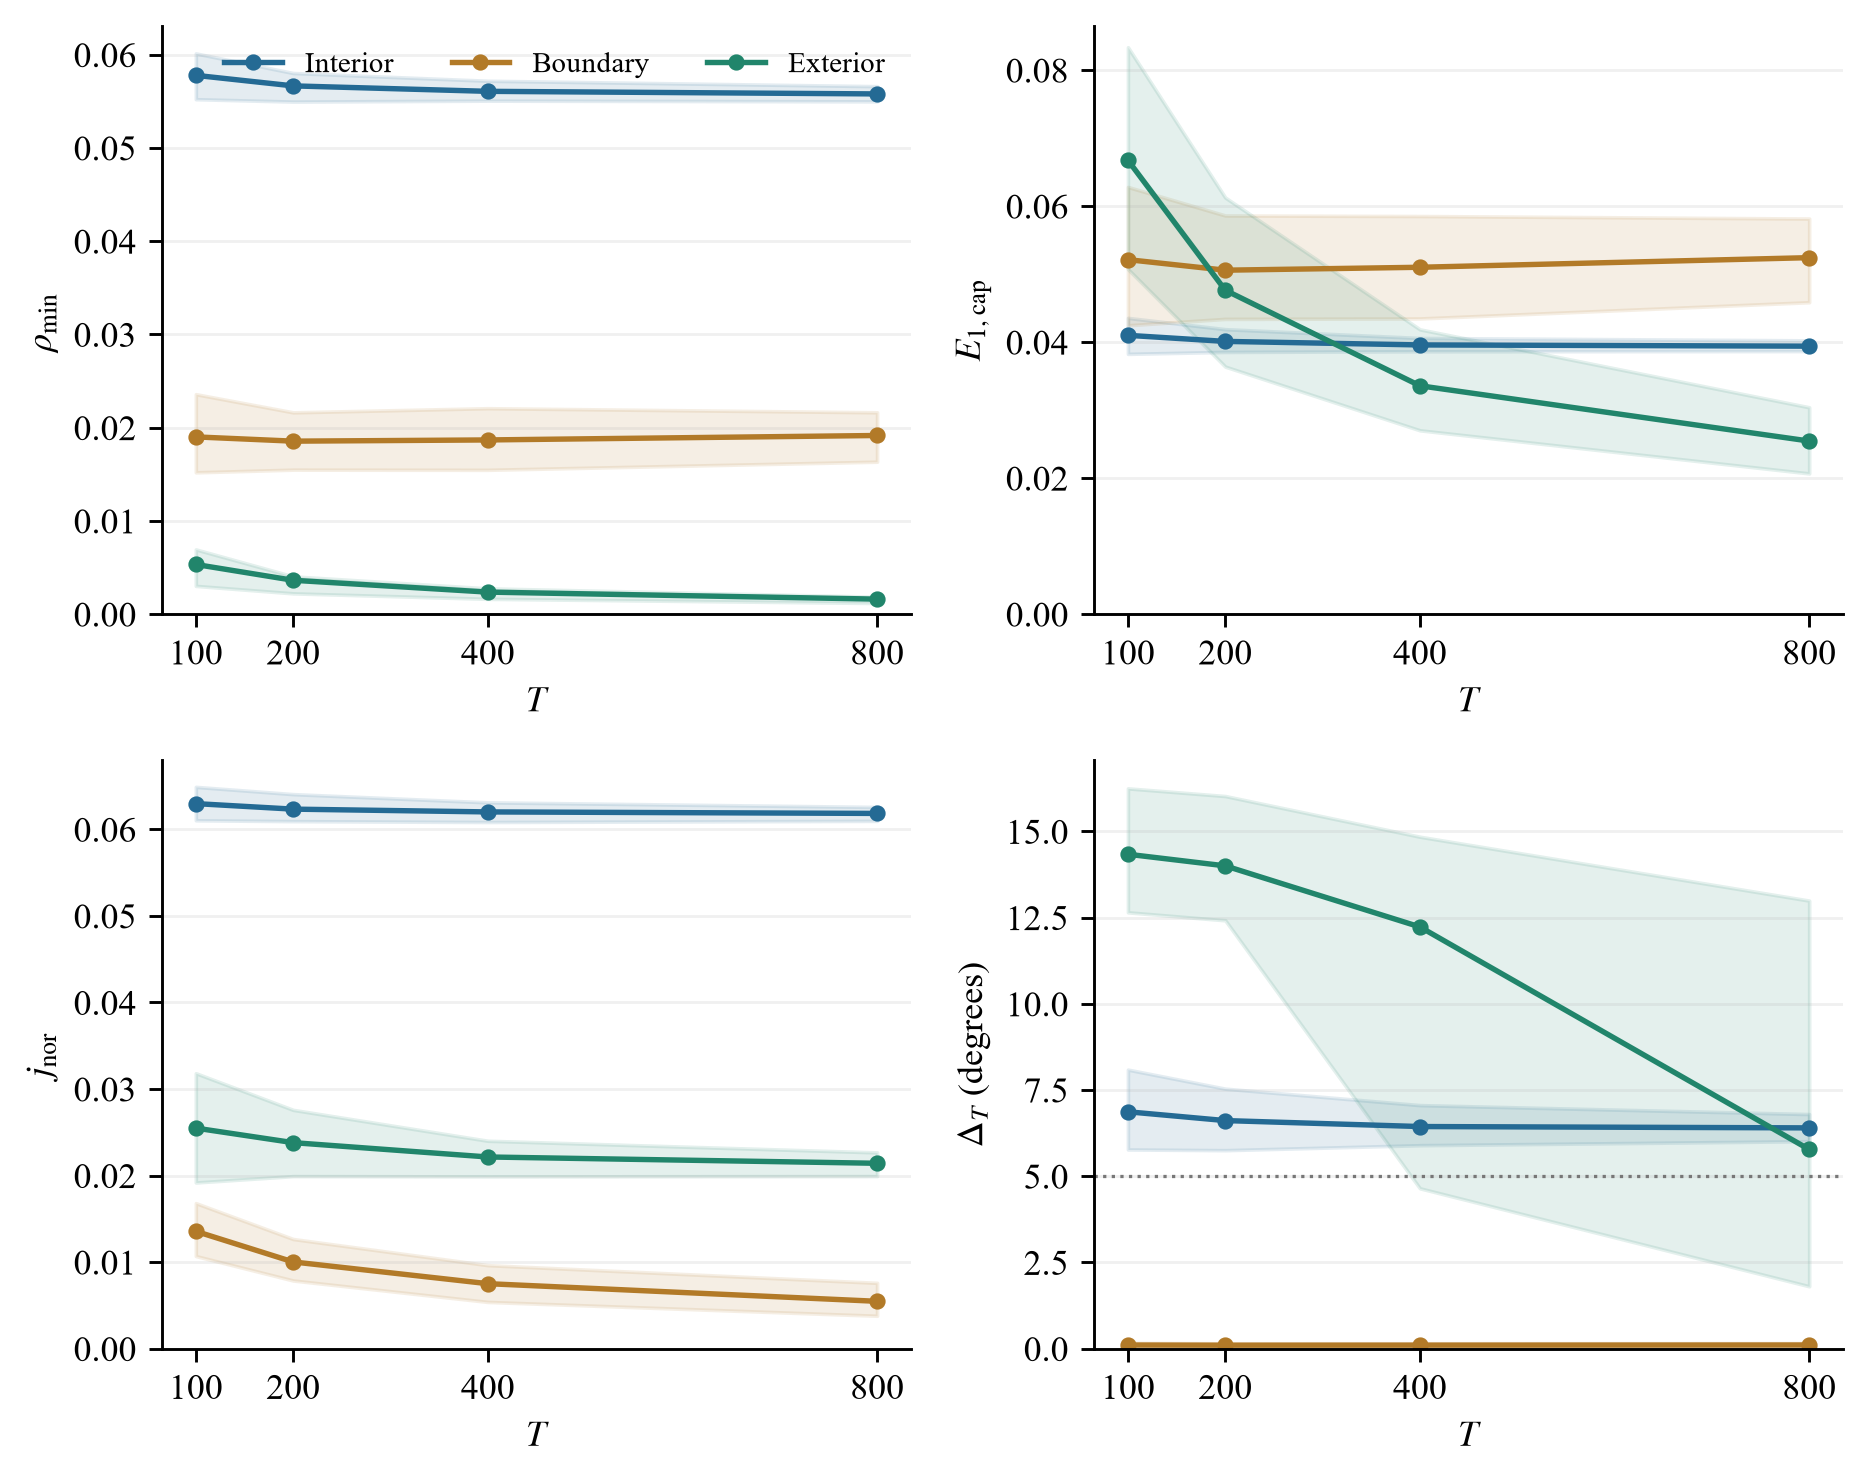
\includegraphics[width=0.98\linewidth,height=0.69\textheight,keepaspectratio]{images/diagnostic_trends_40.png}
\caption{Archived matrix-angle experiment: Diagnostic trends for the diagnostic experiment with $p=q=40$. Lines are means over 100 seeds and shading gives descriptive 10th--90th percentiles, not confidence intervals. The polynomial ratio plotted as $\rho$ in the image is $\rho_{\mathrm{ind}}$, one half of the ratio based on all ordered actual minors. The Jacobian values use the $\psi$-column normalization and depend only on the fitted loadings. The $5^\circ$ cap and independent searches share the archived matrix/loading-cosine threshold $c=0.90$; the dotted line in the angular panel marks $5^\circ$.}
\label{s23:fig:diagnostic_trends}
\endgroup
\end{figure}

\begin{figure}[p]
\begingroup
\spacingset{1.08}
\centering
\setkeys{Gin}{width=!,height=!}
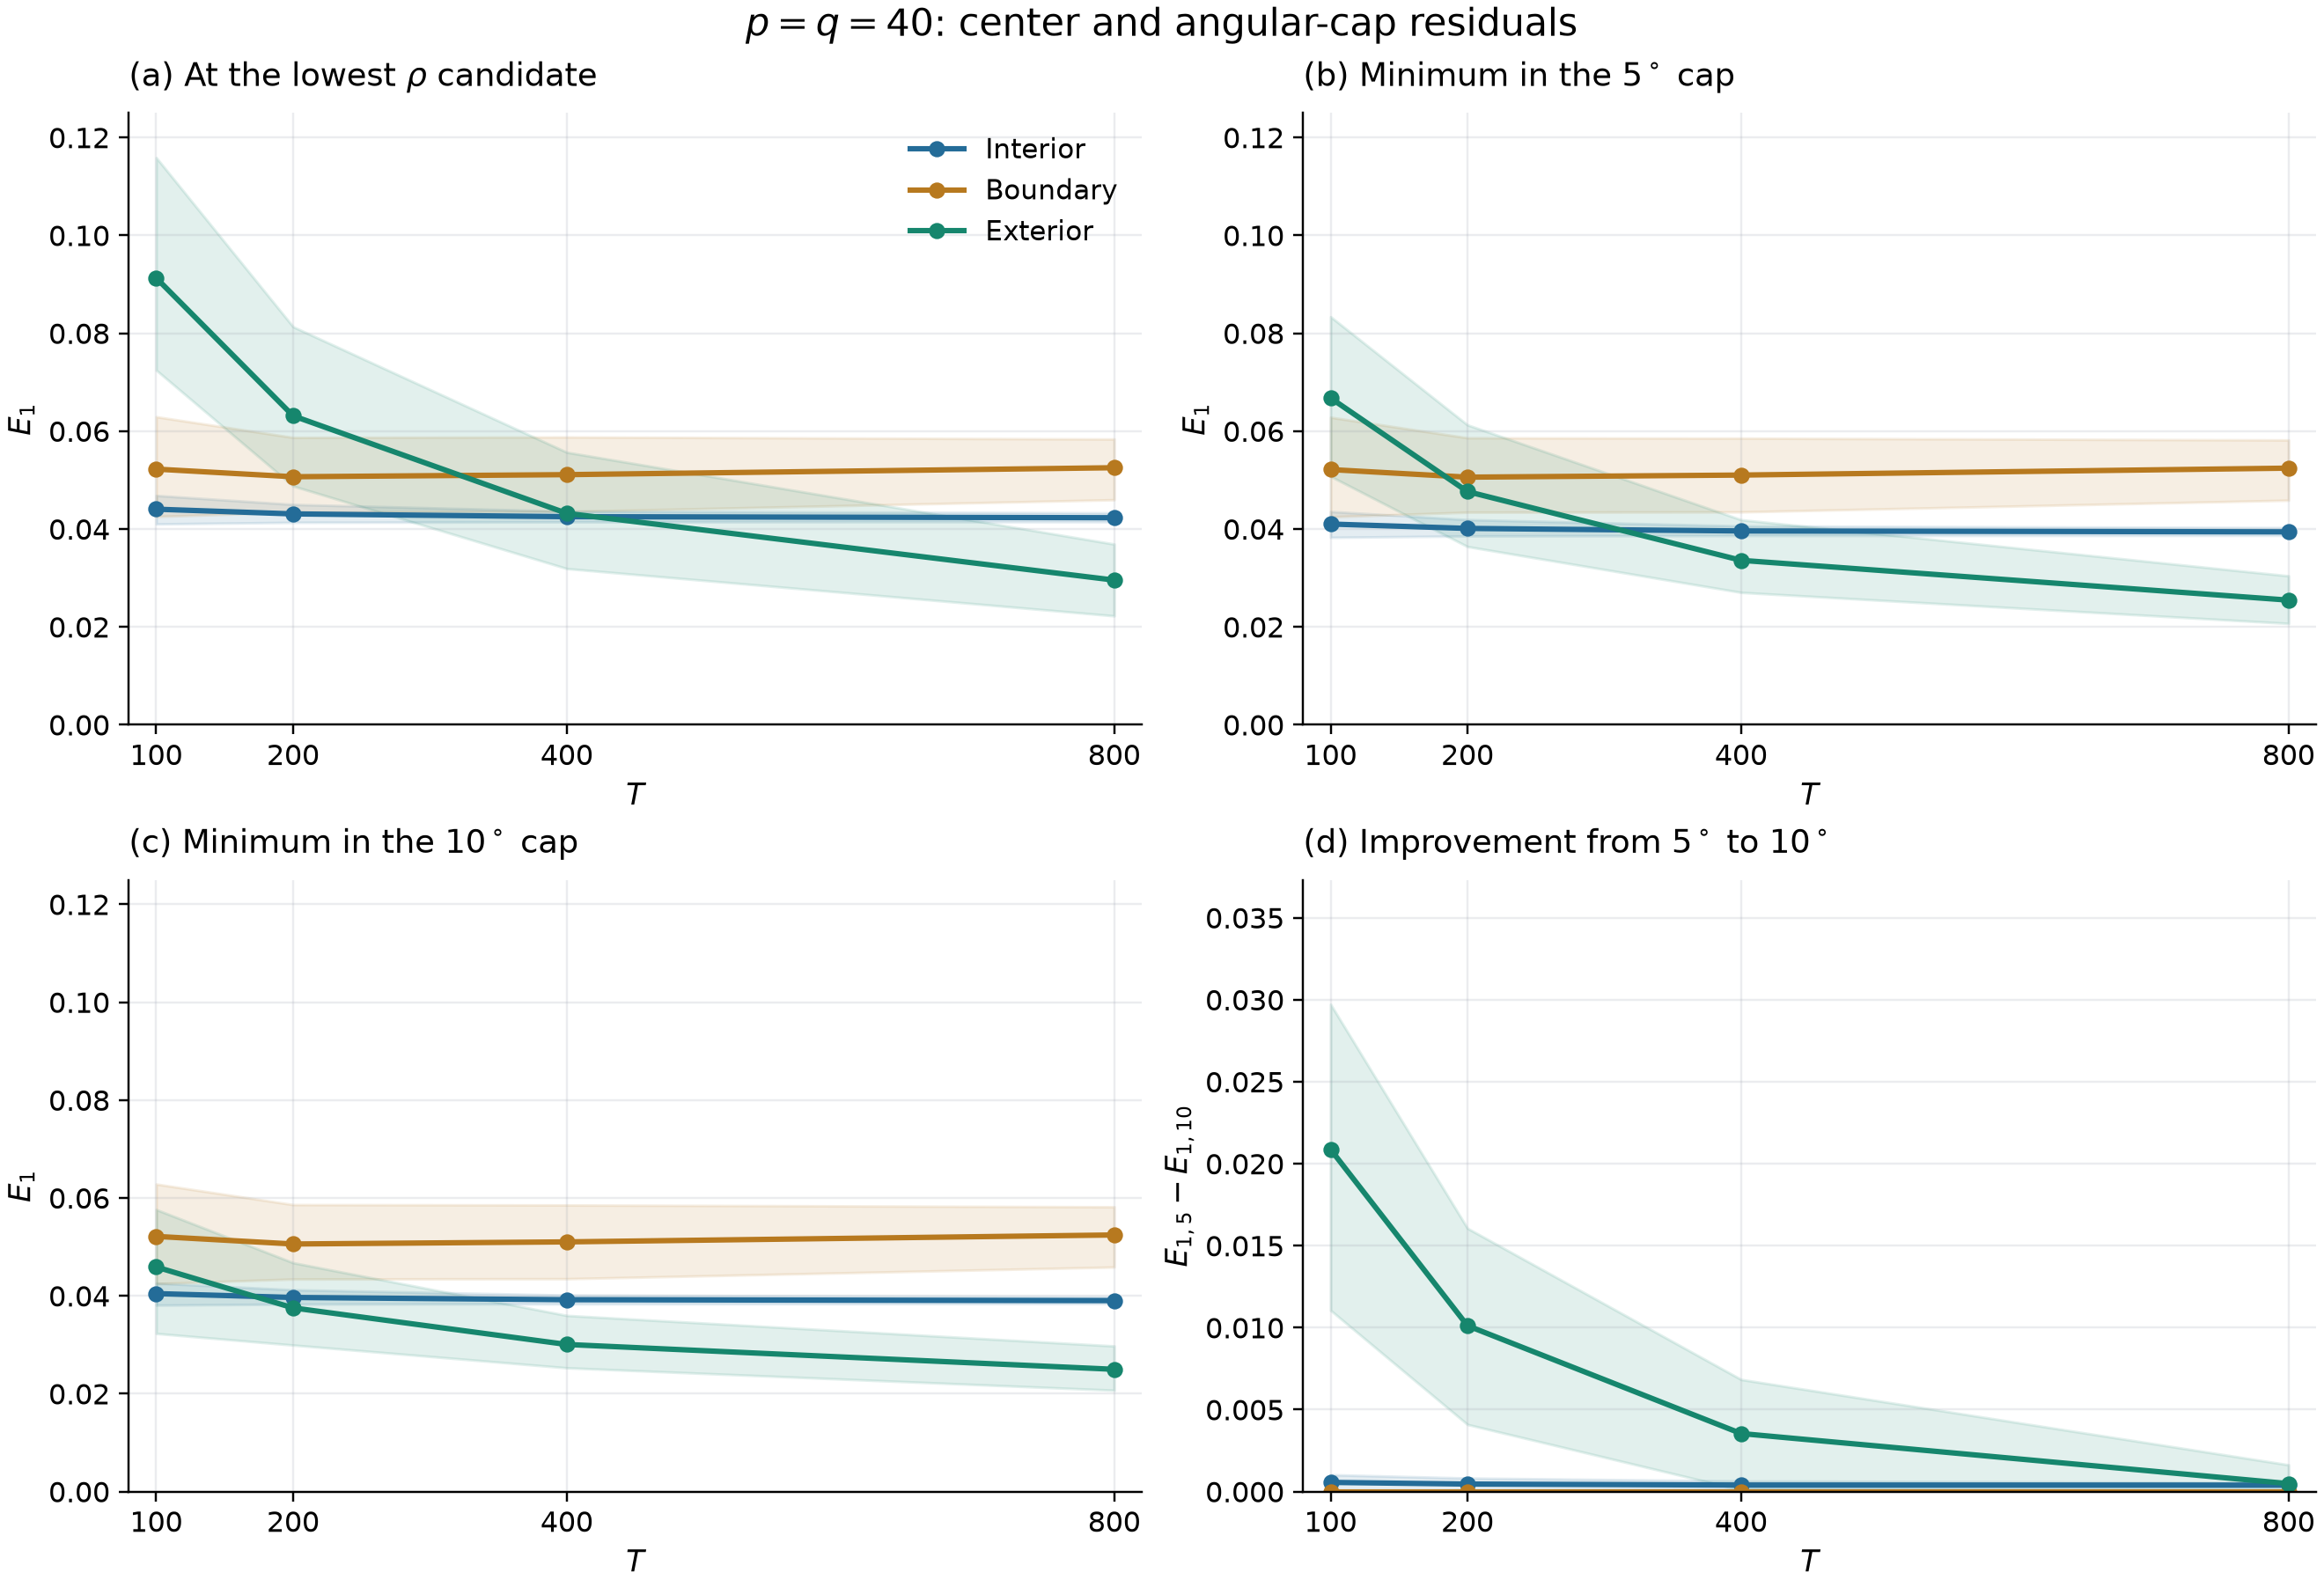
\includegraphics[width=0.98\linewidth,height=0.69\textheight,keepaspectratio]{images/center_5deg_10deg_trends_40.png}
\caption{Archived matrix-angle experiment: Relative rank-one errors at the lowest $\rho_{\mathrm{ind}}$ candidate and within its $5^\circ$ and $10^\circ$ angular caps, for $p=q=40$. Each curve is a mean over 100 seeds; shading gives descriptive 10th--90th percentiles. All searches use the archived matrix-angle domain $\mathcal D^{\mathrm M}_c$ with matrix/loading cosine limit $c=0.90$. The lower-right panel shows $E_{1,5}-E_{1,10}$. Retaining feasible center and $5^\circ$ witnesses enforces the nesting inequality, so a nonnegative improvement is not itself evidence of identification.}
\label{s23:fig:cap_trends}
\endgroup
\end{figure}

\FloatBarrier
\clearpage
\section{Diagnostic trends and selected numerical results}
\label{s23:sec:extended-results}
% Complete primary results from the new lambda-axis-domain searches.
This section summarizes the coefficient-angle experiment defined in
Subsection~S.2.3 of the Supplementary Material. Sections~D.1--D.3 contain the complete numerical listings for
all nine ordered dimension pairs and all four sample sizes. The original QMLE estimates are fixed; every
search-dependent geometric value has been recomputed under
$\max_j|\lambda_j|/\|\lambda\|_2\le0.90$.
The archived comparison in Section~D.4 is explicitly
restricted to the earlier matrix-angle domain. Observed trajectories over four sample sizes
are distinct from proofs of asymptotic limits or convergence rates.

\paragraph{Residual levels and local correspondence.}
Tables~\ref{s23:lambda:selectedtab:cap_comparison}--\ref{s23:lambda:selectedtab:cap_correspondence}
give a compact $40\times40$ comparison. The complete indexed
tables and Figures~D.1--D.7 in Supplementary Data show the
dimension effects.
In the interior, mean $\rho_{\mathrm{ind},\min}$ changes from
$0.057783$ to $0.055792$ as $T$ increases from 100 to 800,
the independent $E_1$ minimum from $0.028499$ to $0.027757$,
and $E_{1,10}$ from $0.038966$ to $0.037520$.
The nearest independent-candidate angle stays near $28.5^\circ$,
and no local $E_1$ candidate is found within $10^\circ$ of the
selected center at $T=800$. These are distinct positive valleys,
consistent with the identified interior construction, despite its
rank-deficient $\Omega$.

The boundary behaves differently on the new domain. At $40\times40$,
mean $\rho_{\mathrm{ind},\min}$ changes from $0.014153$ to
$0.006356$, the independent $E_1$ minimum from $0.007801$ to
$0.003203$, and $E_{1,10}$ from $0.009561$ to $0.003203$.
Mean $\Delta_T$ decreases from $12.082^\circ$ to $0.749^\circ$,
and the found-local-candidate fraction within $10^\circ$ rises
from $41\%$ to $99\%$. At $T=800$ the cap solution is on the
coefficient-axis exclusion boundary in $99/100$ fits, and its
mean physical cosine is $0.994065$. Thus the increasingly close,
deep valleys concern combinations near an existing loading matrix,
although the coefficients remain at least $25.84^\circ$ from
every axis. Close objective minima and small positive residuals
therefore also occur at this identifiable boundary design. At the
population configuration, compactness and identification imply a
strictly positive residual minimum on the fixed exclusion domain;
the observed decrease is not proof of a zero limit.

In the exterior, $40\times40$ mean
$\rho_{\mathrm{ind},\min}$ decreases from $0.005325$ to $0.001609$,
and $E_{1,10}$ from $0.046018$ to $0.024971$.
Mean $\Delta_T$ decreases from $22.151^\circ$ to $9.306^\circ$,
and the local-candidate fraction increases from $3\%$ to $71\%$.
Dimension effects are material: at $T=800$ this fraction ranges
from $25\%$ to $100\%$, and mean $\Delta_T$ from
$1.487^\circ$ to $19.474^\circ$ across the nine pairs.
The interior's corresponding angle range is
$28.472^\circ$--$28.707^\circ$, whereas the boundary's is
$0.030^\circ$--$3.023^\circ$. These finite-sample observations
support different geometric mechanisms, but not a universal rule
that small angle means non-identification.

\paragraph{Why a small polynomial ratio need not give a small center error.}
The identity
$\rho_{\mathrm{ind}}(\lambda)=H(m_r(\lambda))/\|k(\lambda)\|_2$
is important numerically. Unit Frobenius norm of $m_r(\lambda)$
does not bound $\|\lambda\|_2$ uniformly over different loading
maps; nearly cancelling combinations can have large coefficient
products. Consequently, a small ratio can coexist with a few-percent
rank-one error. This is a scale effect of the stated ratio and is
not, by itself, evidence of unsuccessful minimization.
Table~\ref{s23:lambda:tab:denominator} quantifies this mechanism.
At $40\times40$, the exterior mean $\|k(\lambda)\|_2$ at the
selected center decreases from $22.4606$ to $19.4361$ as $T$
increases from 100 to 800, while mean $H/E_1$ increases from
$0.996704$ to $0.999663$. The interior and boundary mean
denominators at $T=800$ are only $0.757529$ and $0.519031$.
The much larger exterior denominator therefore explains why its
ratio can be very small while its center error is still about
$3\%$. These denominator values refer to the unit-Frobenius
normalization, not unit Euclidean coefficient norm.

At $40\times40$, $T=800$, the exterior mean
$(\rho_{\mathrm{ind}},E_1)$ is $(0.001609,0.029548)$ at the
selected center and $(0.002573,0.024971)$ at its $10^\circ$
solution. At the independently lowest $E_1$ candidate the mean pair
is $(0.018724,0.004564)$. These occupy different parts of the
objective landscape. The corresponding boundary pairs are
$(0.006356,0.003276)$ and $(0.006415,0.003203)$ at the center
and cap solution. Hence neither a ranking by $\rho$ alone nor a
ranking by independently minimized $E_1$ alone conveys their joint
behavior. The sample-wise identity involves products; ratios of
the displayed means need not equal a mean denominator.

\paragraph{Coefficient separation and physical matrix proximity.}
The auxiliary physical cosine is especially informative after
changing the domain. At the independently lowest $E_1$ candidate,
all 3,600 boundary fits have $c_{\mathrm{mat}}>0.99$, with mean
about $0.9940$; all 3,596 interior fits and 3,481 of the 3,600
exterior fits have $c_{\mathrm{mat}}>0.90$.
These are valid coefficient-separated candidates, rather than
constraint violations. However, their small errors do not by
themselves exhibit a well-separated additional matrix direction.
At the exterior $40\times40$, $T=800$ cap solution,
mean $c_{\mathrm{mat}}=0.722566$, while the independent minimum
has mean $0.989538$. The physical proximity and the cross-objective
values explain why the two minima deserve separate reporting.
The pooled counts are descriptive: shared seeds across dimensions
do not create 900 independent replications per sample size.

The exterior population construction nevertheless has an exact
additional rank-one direction within the new domain. Direct checks
of all six bases formed by omitting one of the six rank-one
directions give nearest-axis angles $34.06^\circ$--$49.21^\circ$
for the omitted direction. Thus the cutoff $25.84^\circ$ does not
exclude that population zero in these bases. The finite-sample
residuals do not show that it has disappeared: fitted loading spaces
can contain only the given exact rank-one directions even while
approaching the population space. In particular, if both fitted
cores have full column rank, left inverses imply
$\operatorname{rank}\{A_r\operatorname{diag}(\lambda)B_r^\top\}
=|\operatorname{supp}\lambda|$.
This concerns rank-one directions in a loading span, not a proof
of global covariance identification with unknown diagonal noise.

\paragraph{Joint scores, spectra and recovery.}
The joint score is computed from the complete Cartesian product
of the two independent numerical candidate pools. Only one fit,
exterior $(p,q)=(80,20)$, $T=200$, seed 77, has no pair within
$5^\circ$; its $Q_T=+\infty$ is retained in AUCs and excluded
only from conditional finite means, with counts reported.
At $40\times40$, $T=800$, finite mean $Q_T(5^\circ)$ is
$0.109070$, $0.007263$ and $0.018499$ for interior, boundary
and exterior, respectively. The score separates the interior in
these designs, but the boundary can have a smaller joint residual
than the exterior. Its scale is exploratory and uncalibrated.

The $J_\ell$ spectra are unaffected by changing the search domain.
At $40\times40$, mean $j_{\mathrm{orig}}$ changes from
$0.088762$ to $0.087282$ in the interior, from $0.018589$ to
$0.007498$ at the boundary, and from $0.018006$ to $0.015270$
in the exterior. The boundary's decreasing smallest singular value
is a local axis-degeneracy signature; an exterior loading span can
instead have nondegenerate axis Jacobians and an extra remote
rank-one direction. A mixed distribution of alternative fitted
bases is not interpreted as convergence to the original ordered
population columns. All singular values of every $J_\ell$, both
\texttt{orig} and seed-wise normalized \texttt{nor}, are tabulated
in Supplementary Data.
Exterior $40\times40$ mean subspace and relative covariance errors
decrease from $0.050096$ to $0.017444$ and from $0.195613$ to
$0.070662$, respectively. These unchanged recovery summaries are
compatible with estimation improvement, but four sample sizes
alone do not establish consistency.

\paragraph{Interpreting the complete grid.}
Table~\ref{s23:lambda:selectedtab:cap_auc} and the nine full AUC
tables in Supplementary Data retain weak and reversed orderings
as well as strong ones.
For exterior smaller than interior, $E_{1,10}$ AUC ranges from
$0.1460$--$0.5719$ at $T=100$ to $0.9297$--$1$ at $T=800$.
For exterior smaller than boundary, the same AUC is only
$0$--$0.0085$ at $T=800$. Independently minimized $E_1$ likewise
has exterior--boundary AUC $0.0176$--$0.2058$ at $T=800$.
Thus improved interior--exterior separation with $T$ coexists with
a reversed boundary--exterior residual ordering on this domain.
Bootstrap intervals and paired $10^\circ$-versus-$5^\circ$ AUC
changes use 1,000 resamples of the 100 shared seed indices, with
common weights across dimensions and regimes. They are exploratory
and have no multiplicity adjustment. Complete empirical ordering
does not establish zero population classification error.

\par\medskip\noindent\textit{Additional-iteration sensitivity on the new domain.} We recomputed the $\mathcal D^\lambda_{\delta_0}$ searches on 28 previously saved continued QMLE fits, after a common additional budget of 1,300 iterations, and on three separately saved adaptive stress fits. No likelihood optimization was performed in this reassessment. The original and continued fits use the same new-domain search budgets and case-specific random seeds. These configurations were selected purposively; the 15 $T=800$ cases comprise six boundary, four exterior, and five interior cases, pooled across their audited dimensions. They are not a fresh Monte Carlo sample or a higher-budget rerun of the full grid. Table~\ref{s23:lambda:selectedtab:cap_iteration} reports their paired residual changes.

Replacing only these 15 records in the full $T=800$ grid leaves every center/$5^\circ$/$10^\circ$ AUC and its cross-regime ordering matrix unchanged. The $j_{\mathrm{orig}}$, $j_{\mathrm{nor}}$, and $\Delta_T$ AUCs are also unchanged. The largest AUC changes among $\rho_{\mathrm{ind},\min}$, independent $(E_1)_{\min}$, and $Q_T$ are $0.0006$, $0.0001$, and $0.0005$, respectively. Thus the residual-based $T=800$ separation of these fixed designs survives the audited continuation, even though some boundary residuals move appreciably. The smaller-sample stress results are less stable: for the 13 common $T=100$ cases the largest individual $E_{1,10}$ change is $0.01472$, and the corresponding largest full-grid AUC change is $0.0029$ ($0.0099$ for some other scores). The three adaptive exterior stress cases remain a separate comparison. No continued fits were available at $T=200$ or $400$, so this audit supports the stated large-$T$ empirical separation without establishing optimization adequacy for every configuration.

\clearpage
\begin{table}[p]
\begingroup
\spacingset{1.0}
\small\centering
\caption{Paired original and continued-fit diagnostics on $\mathcal D^\lambda_{\delta_0}$. Entries are mean [sample variance] over the same audited fits; the final column is the largest individual absolute change.}
\label{s23:lambda:selectedtab:cap_iteration}
\footnotesize
\setlength{\tabcolsep}{4pt}
\renewcommand{\arraystretch}{1.03}
\textit{Panel A: 15 common-budget $T=800$ cases.}\par\smallskip
\begin{adjustbox}{max width=\linewidth}
\begin{tabular}{llrccc}
\toprule
Design & Score & $n$ & Original & Continued & $\max|\mathrm{change}|$\\
\midrule
Interior & $E_{1,\mathrm{center}}$ & 5 & \shortstack{0.042729\\[-1pt]{\scriptsize[3.59e-07]}} & \shortstack{0.042721\\[-1pt]{\scriptsize[3.71e-07]}} & 0.000039\\
Interior & $E_{1,5}$ & 5 & \shortstack{0.039829\\[-1pt]{\scriptsize[2.99e-07]}} & \shortstack{0.039821\\[-1pt]{\scriptsize[3.08e-07]}} & 0.000034\\
Interior & $E_{1,10}$ & 5 & \shortstack{0.037964\\[-1pt]{\scriptsize[2.66e-07]}} & \shortstack{0.037958\\[-1pt]{\scriptsize[2.74e-07]}} & 0.000030\\
\addlinespace
Boundary & $E_{1,\mathrm{center}}$ & 6 & \shortstack{0.002897\\[-1pt]{\scriptsize[4.31e-07]}} & \shortstack{0.002548\\[-1pt]{\scriptsize[3.17e-07]}} & 0.001170\\
Boundary & $E_{1,5}$ & 6 & \shortstack{0.002868\\[-1pt]{\scriptsize[4.83e-07]}} & \shortstack{0.002521\\[-1pt]{\scriptsize[3.43e-07]}} & 0.001170\\
Boundary & $E_{1,10}$ & 6 & \shortstack{0.002868\\[-1pt]{\scriptsize[4.83e-07]}} & \shortstack{0.002521\\[-1pt]{\scriptsize[3.43e-07]}} & 0.001170\\
\addlinespace
Exterior & $E_{1,\mathrm{center}}$ & 4 & \shortstack{0.026411\\[-1pt]{\scriptsize[5.45e-05]}} & \shortstack{0.026409\\[-1pt]{\scriptsize[5.45e-05]}} & 0.000008\\
Exterior & $E_{1,5}$ & 4 & \shortstack{0.022951\\[-1pt]{\scriptsize[1.80e-05]}} & \shortstack{0.022948\\[-1pt]{\scriptsize[1.80e-05]}} & 0.000011\\
Exterior & $E_{1,10}$ & 4 & \shortstack{0.022434\\[-1pt]{\scriptsize[1.12e-05]}} & \shortstack{0.022430\\[-1pt]{\scriptsize[1.12e-05]}} & 0.000011\\
\addlinespace
\bottomrule
\end{tabular}
\end{adjustbox}
\par\smallskip
\textit{Panel B: $T=100$ common-budget and separate adaptive stress cases.}\par\smallskip
\begin{adjustbox}{max width=\linewidth}
\begin{tabular}{llrccc}
\toprule
Comparison & Design & $n$ & Original $E_{1,10}$ & Continued $E_{1,10}$ & $\max|\mathrm{change}|$\\
\midrule
Common & Interior & 4 & \shortstack{0.037204\\[-1pt]{\scriptsize[2.07e-06]}} & \shortstack{0.037211\\[-1pt]{\scriptsize[2.12e-06]}} & 0.000051\\
Common & Boundary & 3 & \shortstack{0.012319\\[-1pt]{\scriptsize[8.19e-05]}} & \shortstack{0.012322\\[-1pt]{\scriptsize[8.21e-05]}} & 0.000013\\
Common & Exterior & 6 & \shortstack{0.033034\\[-1pt]{\scriptsize[3.49e-04]}} & \shortstack{0.031149\\[-1pt]{\scriptsize[3.56e-04]}} & 0.014716\\
Adaptive & Exterior & 3 & \shortstack{0.020476\\[-1pt]{\scriptsize[1.71e-04]}} & \shortstack{0.016804\\[-1pt]{\scriptsize[4.07e-05]}} & 0.014726\\
\bottomrule
\end{tabular}
\end{adjustbox}
\par\smallskip
\begin{minipage}{0.98\linewidth}\footnotesize
Panel A uses the 15 common-budget configurations at $T=800$; Panel B uses 13 different common-budget configurations at $T=100$ and three additional adaptive continuation records for selected exterior stress cases. Adaptive and common rows are not pooled. The original full-grid means are retained in all main tables. Each diagnostic was newly optimized on the coefficient-angle domain; no historical matrix-domain geometric score is substituted. The same $E_1$ and singular-value scales are used throughout, without squaring or multiplication by 100. The common-budget continuation is additional to the original regime-specific QMLE caps. No continued-fit audit exists at $T=200,400$.
\end{minipage}
\endgroup
\end{table}

% Selected new lambda-domain comparisons; no unrecomputed continuation-geometry table.
\clearpage
\begin{table}[p]
\begingroup
\spacingset{1.0}
\small\centering
\caption{Rank-one errors at the lowest $\rho_{\mathrm{ind}}$ candidate and in its angular neighborhoods on $\mathcal D^\lambda_{\delta_0}$, $p=q=40$. Entries are mean [sample variance] over 100 seeds.}
\label{s23:lambda:selectedtab:cap_comparison}
\footnotesize
\setlength{\tabcolsep}{4pt}
\renewcommand{\arraystretch}{1.03}
\begin{adjustbox}{max width=\linewidth}
\begin{tabular}{lrccc}
\toprule
Design & $T$ & $E_{1,\mathrm{center}}$ & $E_{1,5}$ & $E_{1,10}$\\
\midrule
I & 100 & \shortstack{0.044036\\[-1pt]{\scriptsize[5.26e-06]}} & \shortstack{0.040949\\[-1pt]{\scriptsize[4.19e-06]}} & \shortstack{0.038966\\[-1pt]{\scriptsize[3.99e-06]}}\\
I & 200 & \shortstack{0.043073\\[-1pt]{\scriptsize[2.32e-06]}} & \shortstack{0.040096\\[-1pt]{\scriptsize[1.85e-06]}} & \shortstack{0.038170\\[-1pt]{\scriptsize[1.73e-06]}}\\
I & 400 & \shortstack{0.042506\\[-1pt]{\scriptsize[8.85e-07]}} & \shortstack{0.039586\\[-1pt]{\scriptsize[6.93e-07]}} & \shortstack{0.037684\\[-1pt]{\scriptsize[6.32e-07]}}\\
I & 800 & \shortstack{0.042294\\[-1pt]{\scriptsize[5.91e-07]}} & \shortstack{0.039401\\[-1pt]{\scriptsize[4.74e-07]}} & \shortstack{0.037520\\[-1pt]{\scriptsize[4.48e-07]}}\\
\addlinespace
B & 100 & \shortstack{0.012759\\[-1pt]{\scriptsize[3.08e-05]}} & \shortstack{0.010858\\[-1pt]{\scriptsize[1.75e-05]}} & \shortstack{0.009561\\[-1pt]{\scriptsize[1.07e-05]}}\\
B & 200 & \shortstack{0.006849\\[-1pt]{\scriptsize[4.83e-06]}} & \shortstack{0.006079\\[-1pt]{\scriptsize[2.83e-06]}} & \shortstack{0.005716\\[-1pt]{\scriptsize[1.80e-06]}}\\
B & 400 & \shortstack{0.004453\\[-1pt]{\scriptsize[1.14e-06]}} & \shortstack{0.004180\\[-1pt]{\scriptsize[8.04e-07]}} & \shortstack{0.004088\\[-1pt]{\scriptsize[6.37e-07]}}\\
B & 800 & \shortstack{0.003276\\[-1pt]{\scriptsize[4.91e-07]}} & \shortstack{0.003214\\[-1pt]{\scriptsize[4.78e-07]}} & \shortstack{0.003203\\[-1pt]{\scriptsize[4.72e-07]}}\\
\addlinespace
E & 100 & \shortstack{0.091274\\[-1pt]{\scriptsize[6.36e-04]}} & \shortstack{0.066766\\[-1pt]{\scriptsize[3.23e-04]}} & \shortstack{0.046018\\[-1pt]{\scriptsize[1.29e-04]}}\\
E & 200 & \shortstack{0.063113\\[-1pt]{\scriptsize[2.93e-04]}} & \shortstack{0.047632\\[-1pt]{\scriptsize[1.60e-04]}} & \shortstack{0.037551\\[-1pt]{\scriptsize[7.28e-05]}}\\
E & 400 & \shortstack{0.043188\\[-1pt]{\scriptsize[1.17e-04]}} & \shortstack{0.033584\\[-1pt]{\scriptsize[5.63e-05]}} & \shortstack{0.030051\\[-1pt]{\scriptsize[3.41e-05]}}\\
E & 800 & \shortstack{0.029548\\[-1pt]{\scriptsize[4.22e-05]}} & \shortstack{0.025453\\[-1pt]{\scriptsize[2.29e-05]}} & \shortstack{0.024971\\[-1pt]{\scriptsize[1.92e-05]}}\\
\addlinespace
\bottomrule
\end{tabular}
\end{adjustbox}
\par\smallskip
\begin{minipage}{0.98\linewidth}\footnotesize
The axis-exclusion angle is $\delta_0\simeq25.84^\circ$, distinct from the $5^\circ$ and $10^\circ$ neighborhood radii. The center and feasible $5^\circ$ witnesses are retained in the $10^\circ$ search, so $E_{1,10}\le E_{1,5}\le E_{1,\mathrm{center}}$ by construction. Each physical loading-matrix cosine is auxiliary and is not restricted by this domain.
\end{minipage}
\endgroup
\end{table}
\clearpage
\begin{table}[p]
\begingroup
\spacingset{1.0}
\small\centering
\caption{Complementary local and off-axis geometry on $\mathcal D^\lambda_{\delta_0}$ at $p=q=40,T=800$. Entries are mean [sample variance]; counts refer to 100 seeds.}
\label{s23:lambda:selectedtab:cap_correspondence}
\footnotesize
\setlength{\tabcolsep}{3pt}
\renewcommand{\arraystretch}{1.03}
\textit{Panel A: Jacobians and independent-pair correspondence.}\par\smallskip
\begin{adjustbox}{max width=\linewidth}
\begin{tabular}{lccccc}
\toprule
Design & $j_{\mathrm{orig}}$ & $j_{\mathrm{nor}}$ & $Q_T(5^\circ)$ & Finite $Q_T$ & $\Delta_T$ (deg.)\\
\midrule
I & \shortstack{0.087282\\[-1pt]{\scriptsize[7.41e-07]}} & \shortstack{0.061842\\[-1pt]{\scriptsize[4.38e-07]}} & \shortstack{0.109070\\[-1pt]{\scriptsize[1.17e-06]}} & 100/100 & \shortstack{28.673\\[-1pt]{\scriptsize[3.61e-01]}}\\
B & \shortstack{0.007498\\[-1pt]{\scriptsize[4.04e-06]}} & \shortstack{0.005467\\[-1pt]{\scriptsize[2.15e-06]}} & \shortstack{0.007263\\[-1pt]{\scriptsize[1.09e-05]}} & 100/100 & \shortstack{0.749\\[-1pt]{\scriptsize[4.53e+00]}}\\
E & \shortstack{0.015270\\[-1pt]{\scriptsize[6.41e-06]}} & \shortstack{0.021415\\[-1pt]{\scriptsize[4.26e-06]}} & \shortstack{0.018499\\[-1pt]{\scriptsize[3.90e-06]}} & 100/100 & \shortstack{9.306\\[-1pt]{\scriptsize[1.05e+02]}}\\
\bottomrule
\end{tabular}
\end{adjustbox}
\par\smallskip
\textit{Panel B: cap contacts and uncapped local candidates.}\par\smallskip
\begin{adjustbox}{max width=\linewidth}
\begin{tabular}{lccccc}
\toprule
Design & Cap angle (deg.) & Angle edge & $\lambda$-axis edge & Local candidate & Conditional local $E_1$\\
\midrule
I & \shortstack{10.000\\[-1pt]{\scriptsize[4.47e-17]}} & 100/100 & 0/100 & 0/100 & \textemdash\\
B & \shortstack{0.748\\[-1pt]{\scriptsize[4.50e+00]}} & 1/100 & 99/100 & 99/100 & \shortstack{0.003205\\[-1pt]{\scriptsize[4.76e-07]}}\\
E & \shortstack{5.179\\[-1pt]{\scriptsize[1.27e+01]}} & 34/100 & 0/100 & 71/100 & \shortstack{0.023948\\[-1pt]{\scriptsize[2.07e-05]}}\\
\bottomrule
\end{tabular}
\end{adjustbox}
\par\smallskip
\textit{Panel C: physical cosines, reported without exclusion.}\par\smallskip
\begin{adjustbox}{max width=\linewidth}
\begin{tabular}{lccc}
\toprule
Design & $c_{\mathrm{mat}}$ at independent $(E_1)_{\min}$ & $c_{\mathrm{mat}}$ at $E_{1,10}$ & $c_{\mathrm{mat}}>0.90$ at $E_{1,10}$\\
\midrule
I & \shortstack{0.977941\\[-1pt]{\scriptsize[2.79e-08]}} & \shortstack{0.919992\\[-1pt]{\scriptsize[4.38e-06]}} & 100/100\\
B & \shortstack{0.994066\\[-1pt]{\scriptsize[1.18e-08]}} & \shortstack{0.994065\\[-1pt]{\scriptsize[1.20e-08]}} & 100/100\\
E & \shortstack{0.989538\\[-1pt]{\scriptsize[1.32e-04]}} & \shortstack{0.722566\\[-1pt]{\scriptsize[1.32e-02]}} & 0/100\\
\bottomrule
\end{tabular}
\end{adjustbox}
\par\smallskip
\textit{Panel D: all four original singular values of boundary $J_1$.}\par\smallskip
\begin{adjustbox}{max width=\linewidth}
\begin{tabular}{lcccc}
\toprule
$T$ & $s_{1,1}$ & $s_{1,2}$ & $s_{1,3}$ & $s_{1,4}$\\
\midrule
100 & \shortstack{0.018589\\[-1pt]{\scriptsize[1.06e-05]}} & \shortstack{0.649604\\[-1pt]{\scriptsize[4.19e-05]}} & \shortstack{0.990406\\[-1pt]{\scriptsize[2.54e-05]}} & \shortstack{1.372116\\[-1pt]{\scriptsize[3.58e-04]}}\\
800 & \shortstack{0.007498\\[-1pt]{\scriptsize[4.04e-06]}} & \shortstack{0.649464\\[-1pt]{\scriptsize[7.52e-06]}} & \shortstack{0.990815\\[-1pt]{\scriptsize[4.86e-06]}} & \shortstack{1.371461\\[-1pt]{\scriptsize[8.28e-05]}}\\
Population & $0$ & $0.649445$ & $0.990940$ & $1.371430$\\
\bottomrule
\end{tabular}
\end{adjustbox}
\par\smallskip
\begin{minipage}{0.98\linewidth}\footnotesize
$Q_T$ uses independently searched $\rho_{\mathrm{ind}}$/$E_1$ pairs within $5^\circ$, with unmatched cases recorded as $+\infty$ and excluded only from its finite mean and variance. The cap solution has an imposed angular proximity; the local-candidate count additionally requires an uncapped feasible candidate within $10^\circ$. Numerical stopping is not a proof of mathematical local optimality. Physical cosine exceeding $0.90$ is allowed on the new domain. The boundary Jacobian spectra are unchanged fit-only quantities; all values shown are unsquared.
\end{minipage}
\endgroup
\end{table}
\clearpage
\begin{table}[p]
\begingroup
\spacingset{1.0}
\small\centering
\caption{Interior--exterior separation of the new coefficient-angle-domain errors. AUC is fixed as the probability that an exterior score is smaller than an interior score, with half weight for ties.}
\label{s23:lambda:selectedtab:cap_auc}
\footnotesize
\setlength{\tabcolsep}{4pt}
\renewcommand{\arraystretch}{1.03}
\textit{Panel A: all nine dimension pairs at $T=800$.}\par\smallskip
\begin{adjustbox}{max width=\linewidth}
\begin{tabular}{rrccc}
\toprule
$p$ & $q$ & $E_{1,\mathrm{center}}$ & $E_{1,5}$ & $E_{1,10}$\\
\midrule
20 & 20 & 0.5789 & 0.8450 & 0.9297\\
20 & 40 & 0.8455 & 0.9744 & 0.9836\\
20 & 80 & 0.9308 & 0.9895 & 1.0000\\
40 & 20 & 0.7912 & 0.9694 & 0.9968\\
40 & 40 & 0.9830 & 0.9999 & 1.0000\\
40 & 80 & 1.0000 & 1.0000 & 1.0000\\
80 & 20 & 0.7864 & 0.9800 & 0.9973\\
80 & 40 & 1.0000 & 1.0000 & 1.0000\\
80 & 80 & 1.0000 & 1.0000 & 1.0000\\
\bottomrule
\end{tabular}
\end{adjustbox}
\par\smallskip
\textit{Panel B: selected paired changes from $5^\circ$ to $10^\circ$.}\par\smallskip
\begin{adjustbox}{max width=\linewidth}
\begin{tabular}{rrrcc}
\toprule
$p$ & $q$ & $T$ & $\Delta\mathrm{AUC}_{10-5}$ & 95\% bootstrap interval\\
\midrule
40 & 40 & 400 & 0.1212 & [0.0704,0.1829]\\
20 & 20 & 800 & 0.0847 & [0.0389,0.1352]\\
40 & 40 & 800 & 0.0001 & [0.0000,0.0006]\\
\bottomrule
\end{tabular}
\end{adjustbox}
\par\smallskip
\begin{minipage}{0.98\linewidth}\footnotesize
Every $T=800$ group has 100 seeds. Intervals use 1,000 shared-seed block bootstrap resamples and are exploratory, without multiplicity adjustment. The nested feasible sets guarantee nonincreasing pointwise errors, not an increase in AUC. AUC equal to one describes empirical ordering in these fixed designs. These AUC summaries use the original saved fits. The separately recomputed continued-fit sensitivity is reported in its own audit.
\end{minipage}
\endgroup
\end{table}

% New coefficient-angle diagnostic; computed from saved unit-M lambda vectors.
\begin{table}[p]
\begingroup
\spacingset{1.0}
\small\centering
\caption{Direction-dependent scaling of the polynomial ratio on $\mathcal D^\lambda_{\delta_0}$ for $(p,q)=(40,40)$. Entries are mean [sample variance], with 100 seeds in every row. All quantities are evaluated at the lowest found $\rho_{\mathrm{ind}}$ candidate after imposing $\|m_r(\lambda)\|_F=1$.}
\label{s23:lambda:tab:denominator}
\footnotesize
\setlength{\tabcolsep}{4pt}
\renewcommand{\arraystretch}{1.10}
\begin{adjustbox}{max width=\linewidth}
\begin{tabular}{lrcccc}
\toprule
Design & $T$ & $\rho_{\mathrm{ind},\min}$ & $E_{1,\mathrm{center}}$ & $\|k(\lambda)\|_2$ & $H(m_r(\lambda))/E_{1,\mathrm{center}}$\\
\midrule
Identifiable interior & 100 & \shortstack{0.057783\\[-1pt]{\scriptsize[3.78e-06]}} & \shortstack{0.044036\\[-1pt]{\scriptsize[5.26e-06]}} & \shortstack{0.7616\\[-1pt]{\scriptsize[1.06e-03]}} & \shortstack{0.999247\\[-1pt]{\scriptsize[6.60e-09]}}\\
 & 200 & \shortstack{0.056654\\[-1pt]{\scriptsize[1.60e-06]}} & \shortstack{0.043073\\[-1pt]{\scriptsize[2.32e-06]}} & \shortstack{0.7598\\[-1pt]{\scriptsize[4.70e-04]}} & \shortstack{0.999272\\[-1pt]{\scriptsize[2.83e-09]}}\\
 & 400 & \shortstack{0.056070\\[-1pt]{\scriptsize[8.37e-07]}} & \shortstack{0.042506\\[-1pt]{\scriptsize[8.85e-07]}} & \shortstack{0.7576\\[-1pt]{\scriptsize[1.34e-04]}} & \shortstack{0.999287\\[-1pt]{\scriptsize[1.04e-09]}}\\
 & 800 & \shortstack{0.055792\\[-1pt]{\scriptsize[4.51e-07]}} & \shortstack{0.042294\\[-1pt]{\scriptsize[5.91e-07]}} & \shortstack{0.7575\\[-1pt]{\scriptsize[1.04e-04]}} & \shortstack{0.999291\\[-1pt]{\scriptsize[6.94e-10]}}\\
\addlinespace
Identifiable boundary & 100 & \shortstack{0.014153\\[-1pt]{\scriptsize[6.84e-06]}} & \shortstack{0.012759\\[-1pt]{\scriptsize[3.08e-05]}} & \shortstack{0.9224\\[-1pt]{\scriptsize[1.63e-01]}} & \shortstack{0.999932\\[-1pt]{\scriptsize[4.27e-09]}}\\
 & 200 & \shortstack{0.010397\\[-1pt]{\scriptsize[3.44e-06]}} & \shortstack{0.006849\\[-1pt]{\scriptsize[4.83e-06]}} & \shortstack{0.6680\\[-1pt]{\scriptsize[4.58e-02]}} & \shortstack{0.999982\\[-1pt]{\scriptsize[1.89e-10]}}\\
 & 400 & \shortstack{0.007871\\[-1pt]{\scriptsize[2.24e-06]}} & \shortstack{0.004453\\[-1pt]{\scriptsize[1.14e-06]}} & \shortstack{0.5728\\[-1pt]{\scriptsize[1.66e-02]}} & \shortstack{0.999993\\[-1pt]{\scriptsize[1.58e-11]}}\\
 & 800 & \shortstack{0.006356\\[-1pt]{\scriptsize[2.04e-06]}} & \shortstack{0.003276\\[-1pt]{\scriptsize[4.91e-07]}} & \shortstack{0.5190\\[-1pt]{\scriptsize[3.29e-03]}} & \shortstack{0.999996\\[-1pt]{\scriptsize[3.49e-12]}}\\
\addlinespace
Non-identifiable & 100 & \shortstack{0.005325\\[-1pt]{\scriptsize[1.88e-05]}} & \shortstack{0.091274\\[-1pt]{\scriptsize[6.36e-04]}} & \shortstack{22.4606\\[-1pt]{\scriptsize[1.00e+02]}} & \shortstack{0.996704\\[-1pt]{\scriptsize[2.28e-06]}}\\
 & 200 & \shortstack{0.003630\\[-1pt]{\scriptsize[8.31e-06]}} & \shortstack{0.063113\\[-1pt]{\scriptsize[2.93e-04]}} & \shortstack{20.9233\\[-1pt]{\scriptsize[3.46e+01]}} & \shortstack{0.998429\\[-1pt]{\scriptsize[4.90e-07]}}\\
 & 400 & \shortstack{0.002361\\[-1pt]{\scriptsize[2.27e-06]}} & \shortstack{0.043188\\[-1pt]{\scriptsize[1.17e-04]}} & \shortstack{20.1402\\[-1pt]{\scriptsize[1.99e+01]}} & \shortstack{0.999273\\[-1pt]{\scriptsize[1.03e-07]}}\\
 & 800 & \shortstack{0.001609\\[-1pt]{\scriptsize[8.35e-07]}} & \shortstack{0.029548\\[-1pt]{\scriptsize[4.22e-05]}} & \shortstack{19.4361\\[-1pt]{\scriptsize[1.00e+01]}} & \shortstack{0.999663\\[-1pt]{\scriptsize[1.84e-08]}}\\
\bottomrule
\end{tabular}
\end{adjustbox}
\par\smallskip
\begin{minipage}{0.98\linewidth}\footnotesize
Here $k(\lambda)=(\lambda_i\lambda_j)_{i<j}$, $H$ is the Euclidean norm of the distinct $2\times2$ minors, and $H=\rho_{\mathrm{ind}}\|k(\lambda)\|_2$. The ratio $H/E_1$ is computed within each seed before taking its mean. The matrix has unit Frobenius norm; the coefficient vector need not have unit Euclidean norm. No additional exclusion or residual threshold is applied. The much larger exterior denominator explains why a small polynomial ratio can coexist with a visibly larger rank-one error at the same direction. It does not by itself establish an additional exact rank-one direction. The full 108-cell mean/variance table and all per-seed denominators are retained in the accompanying data.
\end{minipage}
\endgroup
\end{table}
\clearpage
\FloatBarrier
\clearpage
\clearpage
\section{Ancillary AUC comparisons for the early finite samples}
\label{s23:lambda:data:auc}
These comparisons summarize ordering of the same numerical scores;
the absolute residual and spectral levels are discussed in
Subsection~S.2.3 of the Supplementary Material.

Table~\ref{s23:lambda:finite:auc} compares the three fixed designs
at $T=100,200$ over all nine ordered dimension pairs.
For a stated direction $X<Y$, empirical AUC is the proportion of
cross-group score pairs with the $X$ score smaller, giving half
weight to ties. The direction is fixed across all cells; AUC below
$1/2$ is displayed rather than reversed to improve the result.
Ranges in this table describe variation across dimensions, not
confidence intervals. Complete means, sample variances and counts are given in the
metric tables of Section~D.1.

The interior design is clearly separated from the other two already
at $T=100$. Its polynomial ratio is larger, with exterior--interior
AUC $0.9940$--$1$ and boundary--interior AUC $1$ throughout the grid.
The independently lowest found $E_1$ has AUC $1$ for both contrasts,
and $j_{\mathrm{nor}}$ has the corresponding AUC ranges
$0.9980$--$1$ and $1$. The absolute margin $j_{\mathrm{orig}}$
and the joint score $Q_T(5^\circ)$ also have AUC $1$ for both
contrasts at this sample size. Selected summaries and further
interpretation are provided in Section~D.5 of the separate
Supplementary Data file, with complete results in Sections~D.1--D.3.
These are empirical contrasts between the specified designs,
including the interior example with an additional rank defect in
$\Omega$; a rank defect in that matrix alone therefore need not
produce the small-residual behavior of the other designs.

Boundary--exterior comparisons depend on the diagnostic. The
exterior polynomial ratio is typically smaller, but the AUC range
is $0.7419$--$0.9726$ at $T=100$, so this is not a uniform
small-sample separation. In contrast, the boundary's normalized
Jacobian margin is smaller than the exterior's with AUC
$0.8291$--$1$ at $T=100$ and $0.9639$--$1$ at $T=200$.
The boundary also has smaller $E_1$ at the selected $\rho$ center
and within its $10^\circ$ neighborhood: for boundary smaller than
exterior, the AUCs are $0.9092$--$0.9930$ and
$0.9349$--$0.9998$, respectively, at $T=100$.
Thus the smaller center or cap residual does not identify the
non-identifiable design. It describes the depth of a valley on the
chosen coefficient-angle domain, where the boundary configuration
can have small positive residuals close to an existing loading
matrix.

The independently lowest $E_1$ does not uniformly distinguish the
boundary from the exterior either. Its exterior-smaller AUC is
$0.5859$--$0.9280$ at $T=100$, and $0.2290$--$0.8464$ at
$T=200$. Likewise, coefficient-angle correspondence has a useful
interior--exterior contrast (AUC $0.8900$--$0.9903$ at $T=100$,
$0.9579$--$1$ at $T=200$), but the boundary also develops close
correspondence. Proximity of positive minima alone is not evidence
of an additional zero.

We therefore use residual levels, cross-objective values and
near-axis spectra together, and retain their trajectories, angular
and axis-boundary contacts and physical matrix cosines in
Section~D.5 of the separate Supplementary Data file. Complete
mean--variance tables, spectra and dimension-grid figures are
provided there in Sections~D.1--D.3.
None of these AUCs is a calibrated identification test. The interior
has $d=8$ and the other designs have $d=5$; these results do not
provide a dimension-independent threshold for arbitrary loading
configurations. The summaries use the common original fit budgets,
with numerical sensitivity assessed separately.

\begin{table}[p]
\begingroup
\spacingset{1.0}
\small\centering
\caption{Early finite-sample separation on the coefficient-angle domain $\mathcal D^\lambda_{\delta_0}$ across all nine ordered dimension pairs. Ranges are the minimum and maximum empirical AUC across pairs; counts indicate AUC at least $0.95$.}
\label{s23:lambda:finite:auc}
\footnotesize
\setlength{\tabcolsep}{4pt}
\renewcommand{\arraystretch}{1.10}
\begin{adjustbox}{max width=\linewidth}
\begin{tabular}{llcccc}
\toprule
Metric & Fixed direction & \multicolumn{2}{c}{$T=100$} & \multicolumn{2}{c}{$T=200$}\\
\midrule
 &  & AUC range & $\ge0.95$ & AUC range & $\ge0.95$\\
$\rho_{\mathrm{ind},\min}$ & $E<I$ & 0.9940--1.0000 & 9/9 & 1.0000--1.0000 & 9/9\\
$\rho_{\mathrm{ind},\min}$ & $E<B$ & 0.7419--0.9726 & 5/9 & 0.7867--0.9804 & 5/9\\
$\rho_{\mathrm{ind},\min}$ & $B<I$ & 1.0000--1.0000 & 9/9 & 1.0000--1.0000 & 9/9\\
\addlinespace
$E_{1,\mathrm{center}}$ & $E<I$ & 0.0299--0.2907 & 0/9 & 0.0400--0.4983 & 0/9\\
$E_{1,\mathrm{center}}$ & $E<B$ & 0.0070--0.0908 & 0/9 & 0.0007--0.0336 & 0/9\\
$E_{1,\mathrm{center}}$ & $B<I$ & 0.9118--1.0000 & 8/9 & 1.0000--1.0000 & 9/9\\
\addlinespace
$E_{1,10}$ & $E<I$ & 0.1460--0.5719 & 0/9 & 0.2409--0.9701 & 1/9\\
$E_{1,10}$ & $E<B$ & 0.0002--0.0651 & 0/9 & 0.0000--0.0102 & 0/9\\
$E_{1,10}$ & $B<I$ & 0.9632--1.0000 & 9/9 & 1.0000--1.0000 & 9/9\\
\addlinespace
Independent $(E_1)_{\min}$ & $E<I$ & 1.0000--1.0000 & 9/9 & 1.0000--1.0000 & 9/9\\
Independent $(E_1)_{\min}$ & $E<B$ & 0.5859--0.9280 & 0/9 & 0.2290--0.8464 & 0/9\\
Independent $(E_1)_{\min}$ & $B<I$ & 1.0000--1.0000 & 9/9 & 1.0000--1.0000 & 9/9\\
\addlinespace
$j_{\mathrm{nor}}$ & $E<I$ & 0.9980--1.0000 & 9/9 & 1.0000--1.0000 & 9/9\\
$j_{\mathrm{nor}}$ & $E<B$ & 0.0000--0.1709 & 0/9 & 0.0000--0.0361 & 0/9\\
$j_{\mathrm{nor}}$ & $B<I$ & 1.0000--1.0000 & 9/9 & 1.0000--1.0000 & 9/9\\
\addlinespace
$\Delta_T$ & $E<I$ & 0.8900--0.9903 & 8/9 & 0.9579--1.0000 & 9/9\\
$\Delta_T$ & $E<B$ & 0.0849--0.6100 & 0/9 & 0.0282--0.2935 & 0/9\\
$\Delta_T$ & $B<I$ & 0.5917--1.0000 & 6/9 & 0.9340--1.0000 & 8/9\\
\addlinespace
\bottomrule
\end{tabular}
\end{adjustbox}
\par\smallskip
\begin{minipage}{0.98\linewidth}\footnotesize
$I$, $B$, and $E$ denote the identifiable interior, identifiable boundary, and non-identifiable designs. For $X<Y$, AUC is the proportion of cross-group score pairs with the first score smaller, with half weight for ties. The same three directions $E<I$, $E<B$, and $B<I$ are used for every metric, sample size, and dimension pair, including weak or reversed orderings. The $0.95$ cutoff is descriptive rather than calibrated. Subscripts $\min$ refer to the lowest feasible numerical candidates found, without a global-optimality certificate. All geometric scores are recomputed on the new $\lambda$-angle domain; $j_{\mathrm{nor}}$ is unchanged because it depends only on the estimated loadings.
\end{minipage}
\endgroup
\end{table}
\FloatBarrier
\end{document}
